\documentclass[10pt,italian,twocolumn,twoside,xdvi,openany,a4paper]{book}
%%------------------------------------------------------------------------------------------------
%% Packages
%%------------------------------------------------------------------------------------------------
\usepackage{newcent}
% \usepackage{multicol}
\usepackage[T1]{fontenc}
% \usepackage{pslatex}
\usepackage{indentfirst}
\usepackage{afterpage}
\usepackage{longtable}
\usepackage{babel}
\usepackage{latexsym}
\usepackage{fancyhdr}
\usepackage{color}
\usepackage{graphicx}
\usepackage{float}
\usepackage{floatflt}
\usepackage{tabularx}

\newif\iffullversion

\fullversiontrue
\input{fullversioncfg}

%%------------------------------------------------------------------------------------------------
%% Page Layout
%%------------------------------------------------------------------------------------------------
\renewcommand\labelitemi[0]{\(\Diamond\)}
%%------------------------------------------------------------------------------------------------
\newcounter{esnum}
\setcounter{esnum}{0}
%%------------------------------------------------------------------------------------------------
\setlength{\paperwidth}{21cm}
\setlength{\paperheight}{29.7cm}
\setlength{\headsep}{3mm}
\setlength{\textwidth}{16.2cm}
%\setlength{\textwidth}{20cm}
\setlength{\voffset}{-25mm}
\oddsidemargin 0mm
\evensidemargin 0mm
%%\addtolength{\voffset}{-0.75in}
\setlength{\hoffset}{0mm}
\setlength{\textheight}{23.5cm}
\setlength{\marginparwidth}{21mm}
\setlength{\marginparsep}{1mm}

\renewcommand{\textfraction}{0.01}
\renewcommand{\topfraction}{0.95}
\renewcommand{\bottomfraction}{0.95}
\renewcommand{\floatpagefraction}{0.7}
\setcounter{totalnumber}{8}
\setcounter{LTchunksize}{50}
%%------------------------------------------------------------------------------------------------
%% Icons
%%------------------------------------------------------------------------------------------------
%%\newsavebox{\mygraphic}\sbox{\mygraphic}{\includegraphics{background_01.eps}}

\newsavebox{\headimgstaffl}\sbox{\headimgstaffl}{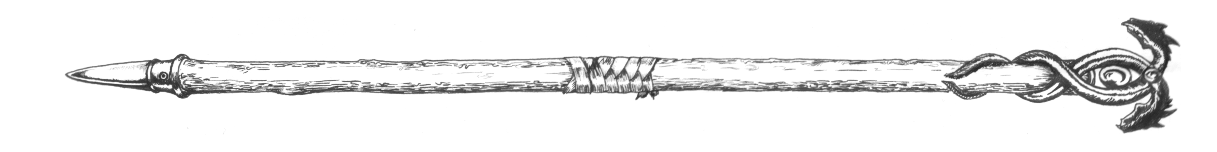
\includegraphics{staff2_l.eps}}
\newsavebox{\headimgstaffr}\sbox{\headimgstaffr}{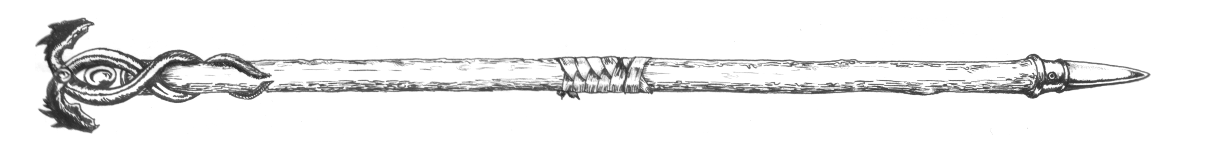
\includegraphics{staff2_r.eps}}
\newsavebox{\headimglandl}\sbox{\headimglandl}{
\includegraphics{paesaggiol.eps}}
\newsavebox{\headimglandr}\sbox{\headimglandr}{
\includegraphics{paesaggior.eps}}
\newsavebox{\headimgwall}\sbox{\headimgwall}{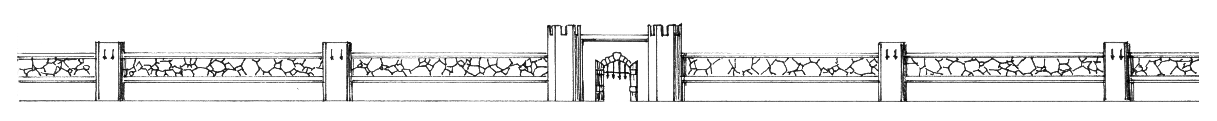
\includegraphics{muraglia.eps}}
\newsavebox{\headimgrune}\sbox{\headimgrune}{
\includegraphics{rune.eps}}
\newsavebox{\headimgpenl}\sbox{\headimgpenl}{
\includegraphics{penninol.eps}}
\newsavebox{\headimgpenr}\sbox{\headimgpenr}{
\includegraphics{penninor.eps}}

\newsavebox{\headimgsword}\sbox{\headimgsword}{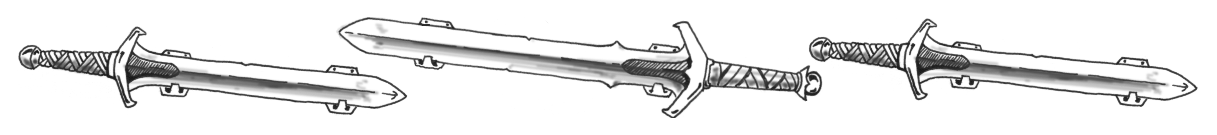
\includegraphics{spade.eps}}

\newsavebox{\footimg}\sbox{\footimg}{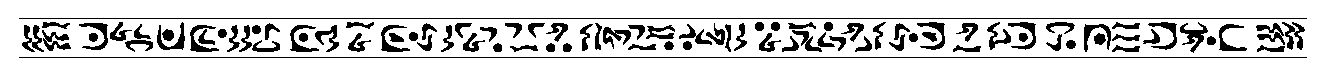
\includegraphics{foot.eps}}
\newsavebox{\iconcorona}\sbox{\iconcorona}{
\includegraphics{icon_corona_small.eps}}
\newsavebox{\iconsacco}\sbox{\iconsacco}{
\includegraphics{icon_sacco_small.eps}}
\newsavebox{\icontiara}\sbox{\icontiara}{
\includegraphics{icon_tiara_small.eps}}
\newsavebox{\iconsfera}\sbox{\iconsfera}{
\includegraphics{icon_sfera_small.eps}}
\newsavebox{\icongiacca}\sbox{\icongiacca}{
\includegraphics{icon_giacca_small.eps}}
\newsavebox{\iconmappa}\sbox{\iconmappa}{
\includegraphics{icon_mappa_small.eps}}
\newsavebox{\iconspada}\sbox{\iconspada}{\includegraphics{icon_spada_small.eps}}
\newsavebox{\iconexcl}\sbox{\iconexcl}{
\includegraphics{icon_excl_small.eps}}
\newsavebox{\icondadi}\sbox{\icondadi}{
\includegraphics{icon_dadi_small.eps}}
\newsavebox{\iconmanosx}\sbox{\iconmanosx}{
\includegraphics{icon_mano_sx_small.eps}}
\newsavebox{\iconmanodx}\sbox{\iconmanodx}{
\includegraphics{icon_mano_dx_small.eps}}
\newsavebox{\iconbobbie}\sbox{\iconbobbie}{
\includegraphics{icon_bobby_small.eps}}

\newlength{\iconoffset}
\newlength{\iconoff}
\newlength{\iconsize}
\settoheight{\iconsize}{\usebox{\icontiara}}

\settoheight{\iconoffset}{Politica}
\setlength{\iconoffset}{4\iconoffset}

\addtolength{\iconoffset}{-\iconsize}
\newcommand{\margintitle}[1]  {\marginpar{\raisebox{\iconoffset}{\usebox{#1}}}}
\newcommand{\margintitles}[2] {\marginpar[\raisebox{\iconoffset}{\usebox{#2}}]{\raisebox{\iconoffset}{\usebox{#1}}}}

\newcommand{\nb}[1] {
  \bigskip\par\nobreak\hrule\nobreak\smallskip\nobreak\indent\textbf{N.B. \margintitles{\iconmanosx}{\iconmanodx} #1}\vskip 3pt plus 0pt\smallskip\hrule
  \smallskip
  }

\iffullversion
\newcommand\topboxl{\usebox{\headimgrune}}
\newcommand\topboxr{\usebox{\headimgrune}}
\else
\newcommand\topboxl{}
\newcommand\topboxr{}
\fi
%%------------------------------------------------------------------------------------------------
%% Head/Foot
%%------------------------------------------------------------------------------------------------
% \advance\marginparpush 3cm
\pagestyle{fancy}
\fancyhead{}
\fancyfoot{}
\fancyhead[RE,LO]{\sc Radix Malorum}

\fancyhead[LE]{\slshape \leftmark}
\fancyhead[RO]{\slshape \rightmark}
\settoheight{\headheight}{X}

\addtolength{\headheight}{20mm}
\renewcommand{\headrulewidth}{1pt}

\fancyhead[CE]{
\setlength{\unitlength}{1cm} 
\begin{picture}(0,0) 
\put(-10,0.8){\topboxl}
\end{picture}}

\fancyhead[CO]{
\setlength{\unitlength}{1cm} 
\begin{picture}(0,0) 
\put(-10,0.8){\topboxr}
\end{picture}}

%%------------------------------------------------------------------------------------------------
%% Lists & Blocks
%%------------------------------------------------------------------------------------------------
\newcommand{\abi}[3] {\goodbreak\noindent\begin{center}\textbf{#1 $\Diamond$ D#2 $\Diamond$
    #3} \end{center}\nopagebreak[4]\par\nopagebreak[4]}

\newcommand{\arm}[3] {\goodbreak\noindent\begin{center}\textbf{#1 $\Diamond$ PP #2 $\Diamond$
    PS #3} \end{center}\nopagebreak[4]\par\nopagebreak[4]}

\newenvironment{radtable}[2]{
  \begin{center}
    
    {\Large\sc #1}\medskip

    \nobreak\begin{tabular}{#2}
      \hline
      }
    {
    \end{tabular}
  \end{center}
  }

\fancyfoot[RO]{
  \vskip 1cm
  \large\it\makebox[5mm]{\thepage\hfil}
}

\fancyfoot[LE]{
  \vskip 1cm
  \large\it\makebox[5mm]{\hfil\thepage}
}

\iffullversion
\fancyfoot[C]{
  \setlength{\unitlength}{1cm} 
  \begin{picture}(0,0) 
    \put(-11.15,-0.7){\usebox{\footimg}}
  \end{picture}
  }
\fi

\newenvironment{esempio} {\begin{figure}[h]\vskip 3pt\small\it\hrule\vskip 3pt} {\vskip 3pt\rm\hrule\end{figure}}
\newenvironment{racconto} {\em\begin{quotation}} {\end{quotation}\em}
\newcommand {\classesoc}[3] {{\noindent\begin{center} #1 $\Diamond$ \textbf{#2} $\Diamond$ FI #3\end{center}}}
\newenvironment{abilist} {\begin{itemize}\itemsep -6pt}{\end{itemize}}

\newcommand{\es}[1] {
  \addtocounter{esnum}{1}
  \medskip\par\noindent\nobreak\framebox[\linewidth][c]{\hfil\sc Esempio \theesnum \hfil}
  \par\medskip\nobreak
  \leftskip 1em
  \rightskip 1em
  {\footnotesize\it\noindent\margintitle{\icondadi} #1\par}
  \par
  \leftskip 0pt
  \rightskip 0pt
  \nobreak\smallskip\nobreak
  \noindent
  \rule{\linewidth}{1pt}\par\smallskip
%%  \smallskip
  }

\newcommand{\pinup}[2] {
  \begin{figure}[tb]
    \begin{center}
      {\it #2}\par
      \includegraphics{#1}
    \end{center}
%%    \caption{#2}
  \end{figure}
  }

\newcommand{\pinupp}[3] {
  \begin{figure}[#3]
    \begin{center}
      {\it #2}\par
      \includegraphics{#1}
    \end{center}
  \end{figure}
  }


\newcommand{\pinupbig}[3] {
  \begin{figure*}[#3]
    \begin{center}
      {\it #2}\par
      \includegraphics{#1}
    \end{center}
  \end{figure*}
  }

\newcommand{\filler}[1]
{
  \begin{figure}[bh]
    \begin{center}
      \includegraphics{#1}
    \end{center}
  \end{figure}
  }

\newcommand{\pinupc}[2] {
%  \begin{figure*}[tbh]
%    \begin{center}
      \includegraphics{#1}
%    \end{center}
%    \caption{#2}
%  \end{figure*}
  }

\newcommand{\demone}[4]{\subsubsection{#1}{\hrule\smallskip\flushright Potenza \textbf{#2} $\Diamond$ #3 \\ #4\smallskip\hrule\medskip\par}}
\newcommand{\angelo}[4]{\subsubsection{#1}{\hrule\smallskip\flushright Potenza \textbf{#2} $\Diamond$ #3 \\ #4\smallskip\hrule\medskip\par}}
\newcommand{\incubo}[4]{\subsubsection{#1}{\hrule\smallskip\flushright Potenza \textbf{#2} $\Diamond$ Incubo di #3 \\ #4\smallskip\hrule\medskip\par}}
\newcommand{\sogno}[4]{\subsubsection{#1}{\hrule\smallskip\flushright Potenza \textbf{#2} $\Diamond$ Sogno di #3 \\ #4\smallskip\hrule\medskip\par}}
\newcommand{\nonmorto}[4]{\subsubsection{#1}{\hrule\smallskip\flushright Potenza \textbf{#2} $\Diamond$ Non Morto \\ #3 $\Diamond$ #4\smallskip\hrule\medskip\par}}
\newcommand{\spirito}[4]{\subsubsection{#1}{\hrule\smallskip\flushright Potenza \textbf{#2} $\Diamond$ Spirito Irrequieto \\ #3 $\Diamond$ #4\smallskip\hrule\medskip\par}}
\newcommand{\anima}[4]{\subsubsection{#1}{\hrule\smallskip\flushright Potenza \textbf{#2} $\Diamond$ Anima Errante\\ #3 $\Diamond$ #4\smallskip\hrule\medskip\par}}
\newcommand{\reombra}[3]{\subsubsection{#1}{\hrule\smallskip\flushright Potenza \textbf{#2} $\Diamond$ #3\smallskip\hrule\medskip\par}}
\newcommand{\elementale}[3]{\subsubsection{#1}{\hrule\smallskip\flushright Potenza \textbf{#2} $\Diamond$ #3\smallskip\hrule\medskip\par}}
\newcommand{\bestia}[4]{\subsubsection{#1}{\hrule\smallskip\flushright Potenza \textbf{#2} $\Diamond$ #4 \\ Habitat: #3\smallskip\hrule\medskip\par}}
\newcommand{\carmostro}[8] {
%% \bigskip\noindent\textbf{Caratteristiche}\medskip
\paragraph{Caratteristiche}
\rightskip 4.5cm
\hfill \ \par\medskip

    INT\hfill #1\par 
    CONC\hfill #2\par
    COS\hfill #3\par
    AGI\hfill #4\par
    FOR\hfill #5\par
    OSS\hfill #6\par
    BEL\hfill #7\par
    PE\hfill #8\par
\rightskip 0cm
}
\newenvironment{parmostro}[1] {\paragraph{#1}\begin{itemize}\itemsep -6pt} {\end{itemize}}

\newenvironment{spell}[4] 
{
    \footnotesize\setlength{\tabcolsep}{1pt}

    \noindent
    \begin{tabular}{*{9}{|p{0.1\linewidth}}|}
     
    \multicolumn{9}{l}{\bf\normalsize #1} \\ \hline
    \multicolumn{9}{r}{#3 $\Diamond$ #4} \\ \hline
    }
  {
    \hline\end{tabular}\par\vfil
  }

\newcommand\parametro[4]{\multicolumn{7}{|l|}{#1: \textbf{#2 #3}}&#4&\  \\ }
%\newcommand\parametro[4]{}

\newcommand\gittata[2]{\multicolumn{7}{|l|}{Gittata: \textbf{#1 m}}&\ &#2\\}

\newcommand\gittatanulla{\multicolumn{7}{|l|}{Gittata: \textbf{a contatto}}&\ &-1\\}

\newcommand\campo[3]{\multicolumn{7}{|l|}{Campo d'azione: \textbf{#1 #2}}&\ &#3\\}

\newcommand\rimbalzi[1]{\multicolumn{7}{|l|}{Rimbalzi: \textbf{#1}}&\ &#1\\}

\newcommand\bonustr[1]{\multicolumn{7}{|l|}{Bonus/Malus TR/TV/TOSS: \textbf{#1}}&\ &#1\\}

\newcommand\durata[2]{\multicolumn{7}{|l|}{Durata: \textbf{#1}}&\ &#2\\}

\newcommand\duratanulla{\multicolumn{7}{|l|}{Durata: \textbf{-}}&\ &0\\}

\newcommand\moddurata[2]{\multicolumn{7}{|l|}{#1}&\ &#2\\ \hline}

\newcommand\azionetempo[2]{\multicolumn{7}{|l|}{Azione nel tempo: \textbf{#1}}&\ &#2\\}
\newcommand\azionegittata{\multicolumn{7}{|l|}{Azione lungo la gittata}&\ &3\\}

\newcommand{\fineparametri}{\hline}

\newcommand\descrizione[1] {
 \multicolumn{9}{|p{0.97\linewidth}|}{\footnotesize\it #1} \\
}
\newcommand\incvalori[9]{\hline 
  \textbf{DR}& \textbf{DA}& TL& \textit{PM}&\textit{PF}&\textit{PE}& DT&\textbf{DB}&MOD\\ 
  \textbf{#1}&\textbf{#2}&#9&\textit{#6}&\textit{#7}&\textit{#8}&#3&\textbf{#4}&#5\\ \hline
}

%%------------------------------------------------------------------------------------------------
%\restylefloat{table}
%\restylefloat{figure}
%\includeonly{michele} %OK
%\includeonly{michele,intro,razze,personaggio,droghe} 
%\includeonly{razze} %OK
%\includeonly{droghe} %OK
%\includeonly{personaggio} % OK
%\includeonly{movimento,droghe} %OK
%\includeonly{movimento}
%\includeonly{combattimento} %OK
%\includeonly{magia} %OK
%\includeonly{scuole} %OK
%\includeonly{incantesimi}
%\includeonly{inc_ele}
%\includeonly{coda}
%%------------------------------------------------------------------------------------------------
%\flushbottom
\fussy
%%------------------------------------------------------------------------------------------------
%% Chapters
%%------------------------------------------------------------------------------------------------
\begin{document}
\thispagestyle{empty}
\begin{titlepage}

\end{titlepage}

\begin{titlepage}
  \begin{center}

%    \iffullversion
%    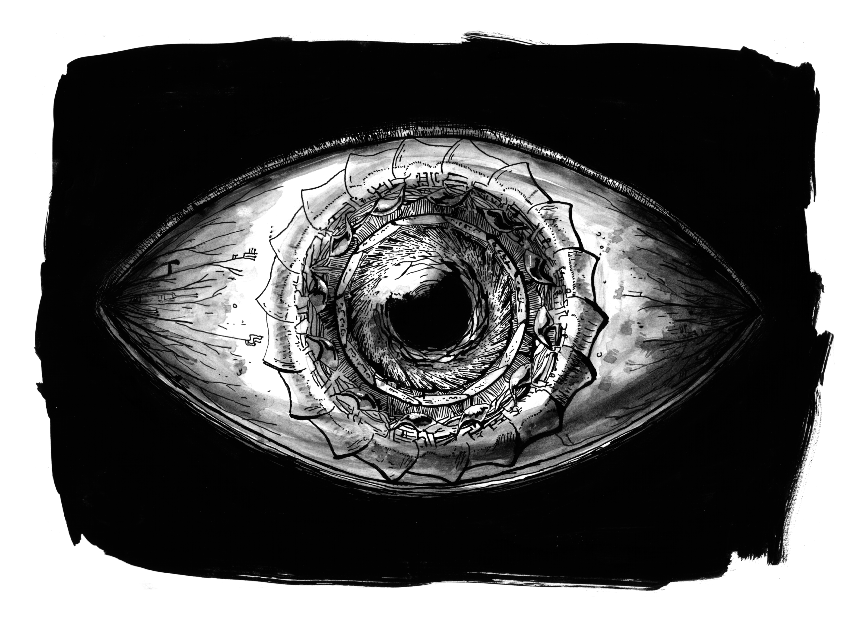
\includegraphics{occhio_big.eps}
%    \else
    
\includegraphics{radixlogo5.eps}
%    \fi

    \vskip 4cm
    \begin{minipage}[c]{16cm}
      \centering
      Juri ``Xeres'' Orr\`u\\Nicola ``Seinen'' Orr\`u\\Sergio ``Alice'' Picciau\\Carlo ``Masamune'' Rosas
    \end{minipage}
    \vskip 1cm

    \begin{minipage}[c]{16cm}
      \centering
\iffullversion
      \Huge\sc Radix Malorum
\else
      \Huge\sc Radix Malorum\\\Large\sc Versione dimostrativa
\fi
    \end{minipage}
  

    \vskip 16cm
    \begin{minipage}[c]{16cm}\it
      \small Hanno collaborato: Salvatore ``Led Lucifer Toti Nexus7'' Saba che ha realizzato i disegni
      dei Simboli delle Scuole; Ocio, Cuccio, Chicco e Saetta che hanno elargito
      moltissimi consigli, alcuni addirittura utili, una moltitudine di playtester, pazienti e divertiti,
      disseminati qua e l\'a per Cagliari. 

      \bigskip
      A tutti, un semplice ma sentitissimo grazie.

      \bigskip
      Con infiniti affetto e nostalgia, al caro amico \textbf{Francesco ``Tanaka Nakatsada'' Mereu.}

      \vskip 6cm

      {\large Licenza d'uso e distribuzione di Radix Malorum}

      \textit{versione 1.0, aprile 2003}
\footnotesize

      \begin{enumerate} \item L'``uso personale'' e la distribuzione
      totale o parziale del materiale contenuto in quest'opera (da qui
      in poi {\bf Radix Malorum}) sono consentite e gratuite per
      ``scopi non commerciali'', fermo restando l'obbligo per il
      distributore e l'utilizzatore di rispettare questa Licenza in
      toto e distribuire integralmente ({\rm verbatim}) il testo di
      questa Licenza in maniera chiara e visibile, insieme a ciascuna
      copia integrale o parziale di {\bf Radix Malorum}.

      \item Gli autori si riservano di revocare la licenza d'uso e
      distribuzione agli utilizzatori e ai distributori che si
      trovassero in contravvenzione di almeno uno degli articoli di
      questa Licenza.

      \item Qualunque utilizzo o distribuzione per ``scopi
      commerciali'' di {\bf Radix Malorum} deve essere esplicitamente
      concordato con gli autori, nelle forme che verranno di volta in
      volta ritenute opportune dagli autori stessi.

      \item Per uso o distribuzione per ``scopi commerciali'' si
      intende qualunque situazione o condizione d'uso che pu\`o
      portare un guadagno, anche indiretto, in termini economici, per
      l'utente o il distributore. Il rimborso spese per il supporto,
      la stampa e la distribuzione non sono da considerare
      ``guadagno'' nella valutazione della ``scopo commerciale''. Per
      uso o distribuzione per ``scopo non commerciale'' si intende
      qualunque situazione o condizione d'uso che non rientra nello
      ``scopo commerciale''. Per ``uso personale'' si intende
      qualunque situazione in cui una singola persona fisica utilizza
      {\bf Radix Malorum} per s\'e, in toto o in parte, senza
      distribuirlo o cederlo a terzi.

      \item Per ``distribuzione'' si intende l'atto con il quale si
      consente a terzi di accedere ad una copia parziale o totale di
      {\bf Radix Malorum}, attraverso qualsiasi mezzo. Sono esempi di
      distribuzione: la trasmissione radiotelevisiva; la duplicazione,
      la stampa, la cessione o la condivisione di un supporto digitale
      o analogico contenente parti di {\bf Radix Malorum}; la
      pubblicazione su una rete informatica o affini di parti di {\bf
      Radix Malorum} che ne consenta la consultazione o la copia a
      pi\'u di una singola persona. Ogni supporto analogico o digitale
      contenente {\bf Radix Malorum} deve contenere una copia
      integrale di questa Licenza.

      \item Gli organizzatori di manifestazioni aperte al pubblico in
      cui si utilizza, si presenta o si distribuisce {\bf Radix
      Malorum}, tra cui tornei, fiere, meeting, ecc., sono vivamente
      pregati (anche se non formalmente obbligati) di contattare
      anticipatamente gli autori, o i loro delegati, per informarli
      circa le modalit\`a di utilizzo e distribuzione di {\bf Radix
      Malorum}, fermi restando i rimanenti articoli della presente
      Licenza.

      \item Tutte le informazioni ufficiali su {\bf Radix Malorum},
      ivi incluse le modalit\`a per contattare direttamente o
      indirettamente gli autori di {\bf Radix Malorum} e le
      informazioni relative alla presente Licenza e alle sue
      successive modifiche, sono accessibili al sito internet
      ufficiale, che pu\'o essere raggiunto via World Wide Web
      all'indirizzo:

      {\tt http://www.radixmalorum.it}

      \item La distribuzione di versioni modificate di {\bf Radix
      Malorum} dovr\`a essere esplicitamente concordata con gli
      autori.

      \item Gli autori di {\bf Radix Malorum} sono (in ordine
      alfabetico): Juri Orr\`u, Nicola Orr\`u, Sergio Picciau e Carlo
      Rosas.

      \end{enumerate} 
\normalsize
\rm
\end{minipage} 
\end{center}
\end{titlepage}
\thispagestyle{empty}
\begin{titlepage}
  \vskip 8cm
\end{titlepage}
\addtocounter{page}{2}

\iffullversion
\renewcommand\topboxl{\usebox{\headimgrune}}
\renewcommand\topboxr{\usebox{\headimgrune}}
\onecolumn
\chapter*{Il Libro}
\begin{racconto}
  ``La stanza era fredda e fiocamente illuminata da tre candele su un
  candelabro di bronzo. La fiamma nel camino si era assopita da tempo
  lasciando alla brace il ruolo di protagonista. Don Michele era
  cos\`{\i} intento a copiare il vecchio testo che non si rese conto
  del suo respiro che si condensava davanti alle pergamene.
  
  La stanza era invasa da ombre che gettavano in ogni angolo un cesto
  di paure. Michele ripeteva sottovoce ci\`o che la sua mano e la
  sua penna andavano vergando sul foglio. Egli non si sarebbe mai
  aspettato di cadere nel baratro della dannazione. Era un servo
  fedele di Ryless, del suo Pontefice e del suo Vescovo, e come suo
  braccio destro credeva d'essere un protetto dal Messia.
  
  Le ombre si condensarono dietro di lui e un vento gelido mosse le
  fiamme delle candele e ravviv\`o i ceppi moribondi del camino. Don
  Michele non si ridest\`o dal suo lavoro mentre i passi silenziosi
  prendevano forma dietro di lui. Una mano gelida si pos\`o sulla
  sua spalla sinistra. Don Michele si volt\`o e il suo urlo, un urlo
  che non emise suono, gli mor\`{\i} in gola. I suoi occhi
  strabuzzarono mentre osservava la figura davanti a lui.
  
  --Chi... Chi Sei?-- mormor\`o
  
  --Ciao, giovane Michele, ti ho spaventato?-- disse la figura, una
  donna bellissima dai capelli rossi avvolta da un sottile velo nero
  che non lasciava niente da immaginare.
  
  --Chi sei, e cosa fai nelle mie stanze, donna?-- rispose con il cuore
  che martellava come un tamburo.
  
  --Donna? Non sono donna pi\`u di quanto non lo sia tu, Michele--
  
  --Che cosa vuoi dire?--
  
  --Troppe domande e tutte inutili, Michele. Piuttosto chiediti cosa
  voglio da te e cosa posso fare per te-- continu\`o la donna
  
  --Cosa vuoi da me?-- chiese allora Michele, stringendo, cos\`{\i} forte
  da farsi sanguinare le mani, il pugnale: il simbolo della morte di
  Ryless.
  
  --Voglio che abbandoni Ryless. Voglio la Chiesa, tutta, ai miei
  ordini.  E voglio che tu sia mio--
  
  --No! Mai! La mia fede \`e grande, pi\`u grande di qualunque
  potere o demone. Esci di qui!--
  
  --Fede??-- La donna inizi\`o a ridere sguaiatamente, ma nessun
  suono usciva dalla stanza.
  
  --Ryless avrebbe desiderato, e lo desidera ancora, un potere come il
  mio.  \`E un debole, non sa neppure ci\`o che accade nei suoi amati
  cieli, non sa neppure cosa tramano i suoi adorati Gabriel e Lucifer,
  \`e un inetto che passa il suo tempo con Antiochio, sorseggiando 
  Phyluf--Herhu tra una partita a carte e una a morra.--
  
  --Menzogne, lui \`e nostro padre e nostra madre; lui \`e la
  nostra guida, la salvezza che ci illumina con la sua grazia!-- si
  difese con forza, Don Michele; ma gi\`a vacillava sull'orlo della
  disperazione.
  
  --Gi\`a, menzogne! Michele, Ryless non ha creato nulla che io non
  possa creare mille volte pi\`u bello e potente. Ti dimenticherai
  di lui, credimi, e noi ci ameremo presto. Mentre attendi, mio
  piccolo amore, scendi nella cripta e apri il sarcofago di San
  Fulgenzio e togli l'elmo dalla sua testa, poi tutto ti si aprir\`a
  davanti. Dopo potrai scegliere il tuo destino--
  
  La donna si accost\`o a don Michele, ormai paralizzato, e lo
  baci\`o sulle labbra.
  
  Le labbra di lei erano di fuoco, roventi come la lava e taglienti
  come rasoi, e risvegliavano i sensi di Michele senza che egli
  potesse opporsi...
  
  Michele si accasci\`o di colpo, come morto. Dorm\`{\i}, sognando
  demoni e partite di carte e la donna dai capelli rossi che nei suoi
  incubi si trasformava in un terribile mostro dai denti aguzzi e
  dalle grandi ali di pipistrello, rosso come il sole al tramonto.
  
  Si ridest\`o ben prima delle odi del mattino, madido di sudore ed
  infreddolito.  Si ritrov\`o a pensare che tutto fosse stato un
  sogno, ma voltandosi nel letto trov\`o sul guanciale una ciocca di
  capelli rossi. Si alz\`o e indoss\`o la tunica e i calzoni, poi
  si avvi\`o verso le cantine. Ud\`{\i} la porta cigolare sinistramente
  ma non ci fece caso. Prese una lanterna dallo scaffale, la
  caric\`o ed accese lo stoppino. Scese silenziosamente sino alla
  cripta. L'umidit\`a era come un peso sulle spalle e rendeva
  difficile la respirazione.
  
  La luce della lanterna era fioca e non dissolveva le tenebre della
  tomba, ma Michele riusc\`{\i} lo stesso a raggiungere il sarcofago
  di granito. Pos\`o la lanterna a terra e spinse con forza. I suoi
  piedi scivolavano sulla muffa del pavimento e le sue unghie si
  spezzavano sul granito mentre il suo sangue cadeva in gocce grosse
  come perle.
  
  Finalmente vide il volto scheletrico di San Fulgenzio, adorno del
  suo elmo.  Il tanfo della morte lo invest\`{\i} come un cavallo in
  carica. Pose le sue mani sull'elmo e lo tir\`o con forza. L'elmo
  si stacc\`o insieme al cranio.
  
  --Ryless, cosa ho fatto!?-- bisbigli\`o, lasciando cadere il teschio
  e portandosi le mani, asciutte e disperate, alla testa.
  
  --Nulla di importante, ma lo hai fatto per me.-- La donna era
  comparsa alle sue spalle, la luce della lanterna non riusciva ad
  illuminarne il volto incorniciato dal rosso crine.
  
  --Mi hai ingannato!-- Inve\`{\i} Michele puntando il dito.
  
  --Su, Su! Non essere permaloso! Avrai ci\`o per cui sei venuto.--
  La donna sorrise mostrando i denti aguzzi. --Ti presento uno dei miei
  servi-- indic\`o l'oscurit\`a --Si chiama Arioch.--
  
  L'ombra vomit\`o un essere alto come un orco, con la pelle rossa e
  striata, le ali di pipistrello e il capo coronato da due corna
  massicce.
  
  --Ciao, Uomo!-- ghign\`o Arioch, mostrando una fila di robustissime
  zanne, bianche come ossa spolpate. Una colonna di fiamme si
  sprigion\`o dalle sue mani. Michele riusc\`{\i} appena in tempo ad
  attivare l'incantesimo di protezione, toccando il suo orecchino
  magico. Fu avvolto dalle fiamme, che lo abbracciarono in mille e
  pi\`u vortici, ma soltanto qualche lembo della sua tunica
  risent\`{\i} degli effetti della fiammata, restando bruciacchiato.
  
  --Dannato demone!-- imprec\`o con rabbia e paura.
  
  --Guarda dietro di te, Uomo!-- grugn\`{\i} il mostro, --Non farmi
  pentire di averti risparmiato--
  
  Michele si volt\`o e vide che si era aperta una crepa nel muro.
  Una luce biancastra filtrava, accompagnata da una sorta di ronzio.
  Michele l'attravers\`o abbacinato.
  
  Mentre i suoi passi rimbombavano nel corridoio, con le mani sfiorava
  le pareti, lisce e fredde, di un metallo mai visto. Di tanto in
  tanto trovava delle strane iscrizioni, dei dipinti con strane forme
  e porte di metallo che non pot\`e aprire in nessun modo.
  
  Cammin\`o per un tempo che gli sembr\`o infinito, finch\'e
  trov\`o il cammino sbarrato da una gigantesca parete di metallo.
  Prov\`o a spingere con tutte le sue forze fino a sentire i muscoli
  di braccia e gambe intorpidirsi.
  
  Poi url\`o. --Ecco! \`E tutto qui ci\`o che doveva distruggere la
  mia fede?-- chiese all'aria che respirava.
  
  --Chiedi aiuto, giovane Michele.-- risuon\`o nella sua mente
  cos\`{\i} forte da costringerlo a tapparsi le orecchie.
  
  --Aiuto, allora. Aiuto!-- ringhi\`o. Una rabbia poderosa, imponente,
  che mai avrebbe sospettato di poter manifestare, si impossess\`o di
  lui.
  
  --Spostati, ammasso di carne urlante.-- brontol\`o con sufficienza,
  spuntando dal nulla, Arioch.
  
  Il mostro colp\`{\i} l'uomo sul petto senza ferirlo, eruttando di nuovo
  le sue fiamme ma ora con tutto il suo potere. Il volto del mostro
  illuminato dal fuoco infernale era una maschera di piacere, dolore e
  follia.
  
  Michele avvert\`{\i} nel petto un caldo opprimente e cap\`{\i} di
  essere stato risparmiato. La parete dietro di lui si sciolse come
  lardo sulla brace.
  
  Un vortice di fumo comparve ed avvolse il Demone, che url\`o con
  odio.
  
  Il fumo si dissip\`o e Michele vide che il Demone era scomparso, e
  che al suo posto c'era ora un oggetto. Un pastorale.
  
  Lo raccolse e lo guard\`o impaurito. l'asta vibrava fra le sue
  mani come percorsa da una strana energia, ed era calda, viva. Lo
  rigir\`o fra le mani e si avvide della somiglianza del suo
  pastorale con quello del Vescovo.
  
  Una luce accecante lo invest\`{\i} e lo distolse dalle sue
  impressioni sul pastorale. Come ipnotizzato si diresse verso la
  fenditura che il demone aveva aperto nella parete. Michele aveva il
  braccio destro davanti a se, disteso, quasi a voler tastare la luce,
  sentirla. Con l'altra mano stringeva il pastorale che continuava a
  muoversi e contrarsi e respirare. La luce era fredda e quasi
  tagliente all'interno di quella enorme stanza.
  
  Davanti agli occhi gli si stagliava un gigantesco, monumentale cilindro
  di metallo che lo guardava con un enorme occhio rosso.
  
  --Quanto tempo \`e passato!-- risuon\`o una voce metallica,
  --Finalmente qualcuno con cui parlare--
  
  --Chi... Cosa?-- balbett\`o Michele
  
  --Io sono la memoria impotente di questo mondo. Io ho visto e
  registrato vita e morte e ricostruzione, e poi ancora vita. Io sono
  il cuore che batte.  Io sono...--
  
  La voce fece una pausa.
  
  --Solo.-- Continu\`o la voce --Da troppo tempo ormai.--
  
  --Ma...-- Michele aveva molte domande, e tutte gli morirono in gola.
  Cosa era quell'essere? Era vivo? Cosa voleva? Da quanto esisteva?
  
  --Io so che sono tante le tue domande, e che il tuo cuore batte
  troppo forte. Ma io non mi ricordo il calore di un essere vivente...
  Avvicinati, e se lo vorrai, ti sveler\`o la Verit\`a.--
  
  Michele si avvicin\`o passo dopo passo, lentamente, mentre il suo
  cuore sembrava non distinguere pi\`u un battito dall'altro. Il
  dimenarsi leggero e caldo del pastorale lo rassicurava. Sentiva il
  fuoco fluire dentro di s\`e.
  
  --Mostramela!-- grid\`o Michele, allargando le braccia. Dalla base
  dell'occhio saettarono migliaia di tentacoli che lo avvolsero come
  una gabbia di rovi e lo percorsero, lo sentirono, e gli mostrarono
  la Verit\`a. La verit\`a disperse il suo cuore. Per Sempre.
  
  Il pastorale cadde dalla sua mano, mentre viveva ci\`o che era
  stato.  Le macchine volanti. La nascita delle razze. L'arrivo di una
  nave dal cielo.  La rabbia della Terra.
  
  Vide colonne di fiamme alte decine di chilometri e nubi nere come
  l'oblio.  Sent\`{\i} il dolore, la paura, le lacrime e l'abbandono
  di un mondo. Url\`o fino a dimenticare quanto. Riemerse dal dolore
  nel suo letto, si sedette e dopo aver dissolto il torpore iniziale
  studi\`o il pastorale fra le mani. Era vivo, non c'era dubbio.
  
  --Arioch!-- chiam\`o. Un vortice di fumo scatur\`{\i} dall'asta, si
  condens\`o e l'Arioch apparve. --Chiama i tuoi demoni. Che scrivano
  ci\`o che mi \`e stato svelato.-- ordin\`o Michele.
  
  Arioch rispose sprezzante: --O forse potrei strapparti la carne a
  poco a poco--
  
  --Chiamali. Te lo ordino.-- ribad\`{\i}.
  
  I loro sguardi si incrociarono. I rossi occhi di Arioch sprizzavano
  fiamme di odio e dolore, che sfidavano la pazzia pura e semplice
  degli occhi azzurri di Michele. Dopo una eterna frazione di secondo
  Arioch chin\`o il capo, si inginocchi\`o e ringhi\`o di
  rabbia:
  
  --Agli ordini, Padrone!--
  
  L'istante successivo apparve un essere orribile, una sorta di
  ammasso cartilagineo dotato di otto arti peduncolati e di uno strano
  tentacolo. Il tentacolo si avvilupp\`o intorno alla testa di
  Michele ed inizi\`o a pulsare. Il Demone inizi\`o a gonfiarsi
  delle memorie del giovane, fino a occupare tutta la stanza. Una
  grossa pustola, ricolma di conoscenza.
  
  Il mostro aracnoide inizi\`o a scrivere, veloce come il vento, e
  mentre scriveva il sapere sui fogli, il suo ventre si sgonfiava.
  
  --Andiamo, ora, andiamo a trovare un defunto-- ghign\`o Michele
  rivolgendosi all'Arioch.
  
  --S\`\i, mio Signore-- rispose l'Arioch, quasi soddisfatto.
  
  Michele si diresse senza alcuna circospezione verso la stanza del
  suo superiore, si accost\`o alla porta salutando la guardia che la
  presidiava.  Il Vescovo di Rylex dormiva ancora.
  
  Michele lo dest\`o dolcemente: --Mia Eccellenza-- salut\`o con un
  inchino.
  
  --Oh, Michele. Perch\'e mi svegli cos\`{\i} presto?-- domand\`o
  assonnato l'anziano Vescovo.
  
  --Un funerale, Eccellenza.-- Michele sfoder\`o un sorriso
  sarcastico.  Il pastorale gli pulsava ancora tra le mani.
  
  --A quest'ora?-- domand\`o sbigottito il vecchio, --E di chi?--
  
  --Il suo, Eccellenza-- Il vecchio non fece in tempo a stupirsi che le
  mani di Michele si levarono. Il corpo del vescovo cominci\`o a
  contrarsi in preda alle convulsioni. Il torace gli si gonfi\`o,
  fino a lacerare la veste, la pelle, la gabbia toracica fino alla
  gola, soffocando i suoi lamenti. Il corpo del vecchio esplose,
  rivoltandosi come un guanto. Di quello che era stato l'arcivescovo
  di Rylex era rimasto un ammasso di visceri e ossa sanguinolente.
  
  Michele richiam\`o il suo Arioch e gli ordin\`o di uccidere la
  guardia all'ingresso. La porta si apr\`{\i} e, mentre Michele usciva,
  la testa della guardia implodeva con uno schiocco sordo sotto la
  stretta dell'Arioch.
  
  --Ora sparisci-- ordin\`o al demone. Michele torn\`o nelle sue
  stanze.  Dove prima c'era il demone gonfio di conoscenza si trovava
  il Libro. Sollev\`o il tomo fra le mani e pronunci\`o un
  vincolo, e poi un altro, e poi un altro ancora, e poi ancora, fino
  quasi a crollare esausto.
  
  --Ecco il Radix Malorum, la Radice di tutti i Mali. Lo custodir\`o
  e nessuno sapr\`a mai la Verit\`a.-- esclam\`o. Tra le nebbie
  della stanchezza che lo sommergevano vide apparire la donna dai
  capelli rossi. Nuda, bella, provocante.
  
  --E tu sarai mio-- disse sorridendo la donna.
  
  --S\`i, mio Signore-- rispose Michele perdendosi nel suo caldo
  abbraccio.''
\begin{figure*}[t]
\begin{center}
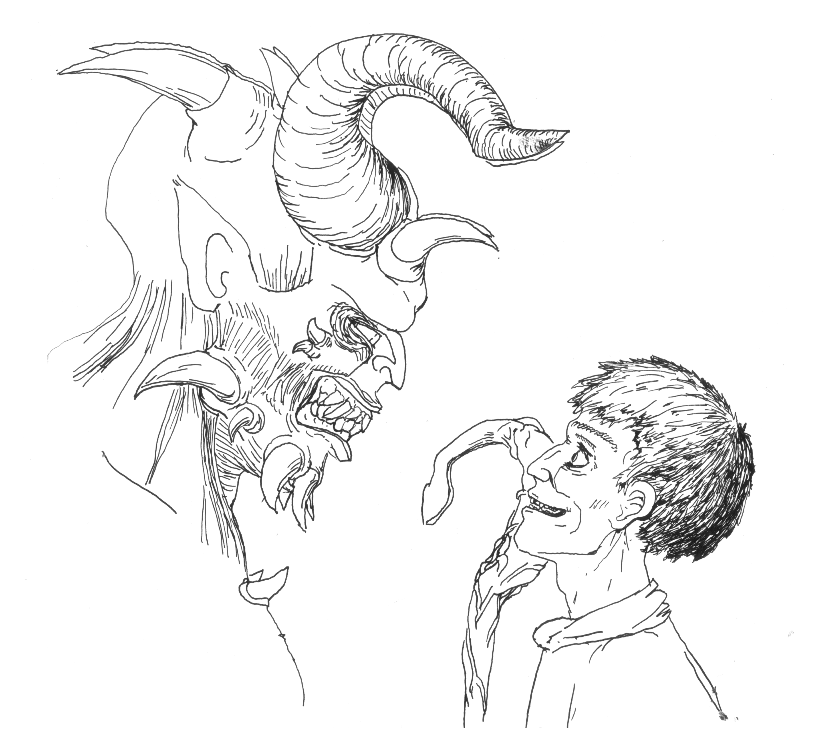
\includegraphics{michele_arioch.eps}
\end{center}
\end{figure*}

\end{racconto}

\twocolumn

%%% Local Variables: 
%%% mode: latex
%%% TeX-master: "manual"
%%% End:
\renewcommand\topboxl{\usebox{\headimglandl}}
\renewcommand\topboxr{\usebox{\headimglandr}}
\fi
%
\chapter{Introduzione}
\section{Prefazione}
%%
\subsection{Cos'\`e un Gioco di Ruolo}
Quello che avete fra le mani e che vi apprestate a leggere \`e il
manuale di un Gioco di Ruolo, che gli addetti ai lavori chiamano {\bf
GdR}. A beneficio di chi non conosce il significato del termine,
forniamo una breve spiegazione.

Il modo pi\`u semplice per descrivere il contenuto e lo scopo del
GdR consiste nell'analizzare il termine stesso ``Gioco di Ruolo''. In
quanto {\bf gioco} in esso \`e predominante l'aspetto ludico e ricreativo
con lo scopo di divertire i partecipanti; il fine principale di ciascuno \`e
quello di interpretare una parte, un {\bf ruolo}, che gli permetta
di calarsi, con l'aiuto della propria fantasia, nei panni di un
personaggio, e di interpretarlo, muovendolo con l'ausilio di regole
all'interno della trama intessuta da un altro giocatore regista.
\iffullversion

Questo mette in evidenza una prima distinzione fra i giocatori:
coloro che si calano nei panni dei cosiddetti Personaggi Giocanti o
{\bf PG}, e colui che crea la storia, la trama all'interno del quale i PG si
muoveranno, come il regista di un'opera. Il ``regista'' nella
maggior parte dei GdR prende il nome di {\bf Master} (o Arbitro, o qualcosa
del genere).

Il GdR esalta la creativit\`a delle persone portandole a
sperimentare i modi di interagire pi\`u adatti alle situazioni in
cui il Master decide di far imbattere i PG. L'interpretazione del
ruolo \`e cardine fondamentale del GdR e non viene sminuita nel
ruolo del Master, il quale non \`e il creatore di una trama sterile
e prestabilita come potrebbe essere quella di un film, ma rappresenta
tutto il mondo dei PG, comprese tutte le persone che i questi potranno
incontrare durante lo svilupparsi del gioco. 

In altre parole, il
Master stende un canovaccio, una trama di cui decide i punti salienti
e i personaggi ``complementari'' che egli dovr\`a gestire (detti
Personaggi Non Giocanti o {\bf PNG}), mentre i giocatori hanno il compito di
sviluppare le linee guida della storia, tramite le proprie azioni, la
reciproca interazione e l'interazione con il Master; il tutto mediante
l'applicazione delle regole che permettono di far vivere e agire i PG,
che restano comunque personaggi di fantasia.
\fi

\subsection{Il GdR Fantasy}

Il gioco di ruolo ha conosciuto nella sua storia adattamenti pi\`u o
meno riusciti a molteplici ambientazioni, reali o parto della fantasia
di autori pi\`u o meno noti, quali Tolkien, Gibson, Rice, solo per
citarne alcuni.

Sul mercato si trovano GdR per tutti i palati: Horror, Gotico,
Fantascientifico, Cyberpunk, Demenziale, Storico ecc. Tuttavia ci
sentiamo di affermare che il genere pi\`u diffuso \`e il Fantasy,
dove storia e fantasia si mischiano in una alchimia elettrizzante,
dove la spada si incrocia con la magia (il classico \textit{Sword \&
  Sorcery}) e in cui abbondano creature fantastiche e mitologiche.

Il progenitore del GdR Fantasy \`e senza dubbio Dungeons \& Dragons,
che ha lanciato una moda e segnato un'epoca.

Il gioco che state per conoscere, \textbf{Radix Malorum}, appartiene a
tale categoria. Esso rispecchia, con le dovute differenze, i capisaldi
del genere fantasy. Radix Malorum \`e, ciononostante, frutto della
fantasia dei suoi autori e la sua ambientazione \`e totalmente
originale e scaturita insieme alle altre regole da un duro lavoro di
sperimentazione durato quasi nove anni, senza negare il contributo
datoci dagli autori che hanno fatto nascere in noi la passione per
questo genere.

{\sloppy\raggedright \subsection{Le caratteristiche di Radix Malorum}}

Fra i punti di forza di Radix Malorum possiamo ricordare:

\begin{itemize}

\item la dettagliata ambientazione \textbf{originale}

\item il sistema di \textbf{miglioramento} delle
abilit\`a, proporzionato alla complessit\`a delle abilit\`a
stesse;

\item il \textbf{sistema di combattimento}, studiato per garantire
un buon equilibrio tra realismo e spettacolarit\`a, in cui anche un
solo colpo di pugnale pu\`o uccidere, in cui \`e prevista la
possibilit\`a per le armature di danneggiarsi e logorarsi, e per le
armi di rompersi; 

\item infine, un sistema di \textbf{creazione immediata
della magia} che permette di attivare incantesimi personalizzati da
adattare ad ogni situazione.

\end{itemize}

Vi sveliamo a questo punto un ``segreto'' che potrebbe soddisfare le
curiosit\`a che sicuramente vi sorgeranno nella lettura: gli autori di
Radix Malorum sono sardi e molto legati alla loro terra. In pi\`u
punti del manuale troverete riferimenti a miti, luoghi e tradizioni
della Sardegna, riferimenti che sono stati ritenuti dagli autori un
doveroso omaggio alla loro isola.

Per scoprire un nuovo meraviglioso mondo, non dovrete far altro che
addentrarvi nella lettura, senza spaventarvi alle prime difficolt\`a
di applicazione delle regole. E vi garantiamo che ne sar\`a valsa la
pena.

%%
{\sloppypar\raggedright \section{Il Mondo di Quadrantal}}
%%
Il mondo in cui vi apprestate ad entrare, per scoprirne misteri,
meraviglie, passioni e paure, \`e stato chiamato, dai suoi abitanti
originali, Quadrantal.  Il nome \textbf{Quadrantal} significa nell'antica
lingua ``dado'', infatti gli indigeni pensavano che esso presentasse
tale forma.

\iffullversion
Attorno a Quadrantal orbitano due satelliti naturali, due lune
chiamate \textbf{Mohwr} e \textbf{Alphan}. La prima appare di colore
rosso, mentre la seconda di colore bianco.

L'anno solare dura 300 giorni. 
\fi

\subsection{L'Arcipelago}

Il cosiddetto ``mondo conosciuto'', chiamato \textbf{Arcipelago},
\`e un continente, situato interamente nell'emisfero settentrionale
del pianeta, costituito da 7 grandi isole disposte in cerchio e
delimitanti un grande specchio d'acqua chiamato \textbf{Mare Interno}.
Al centro del Mare Interno sorge una piccola isola detta Isola del
\textbf{Gran Consiglio}.

Gli abitanti dell'Arcipelago ignorano quanto si trovi nel resto del
pianeta, oltre il cosiddetto \textbf{Mare Esterno}. Questo, infatti,
non \`e da essi navigabile se non nelle immediate vicinanze delle
isole. 

Ogni nazione nell'Arcipelago ha un proprio calendario, ma durante la
\textbf{Dominazione Levante}, per facilitare i fiorenti scambi
commerciali, \`e stato adottato un calendario comune, detto Calendario
Commerciale, utilizzato in tutto il continente, in cui l'anno solare
\`e diviso in 10 mesi di 30 giorni ciascuno.

\iffullversion
I mesi sono: 

\begin{enumerate}\itemsep -6pt
\item Titheea
\item Tebidow
\item Kalhentee
\item Bahska
\item Bowdhyow
\item Proydee
\item Skow-Thowladah
\item Fryow-Sow
\item Nyee
\item Jelhow 
\end{enumerate}

Il passaggio tra le fasce climatiche non \`e netto, ma graduale. \`E
possibile comunque individuare quattro fasce principali.

Nella \textbf{zona artica} la temperatura \`e sempre molto bassa e
non piove mai, perch\'e nevica.

Nella \textbf{zona fredda} i mesi 1,2,9,10 sono invernali, 3,4
primaverili, 5 estivo e 6,7,8,9 autunnali. Le precipitazioni sono
distribuite pi\`u o meno uniformemente su tutto l'arco dell'anno.

Nella \textbf{zona temperata} le stagioni sono ben definite, i mesi
1,9,10 sono invernali, 2 e 3 primaverili, 4,5,6 estivi e 7,8
autunnali. La stagione estiva \`e secca.  l'alternarsi delle
stagioni \`e graduale.

Nella \textbf{zona tropicale}, in cui la temperatura \`e sempre
alta, esistono soltanto due stagioni, la stagione secca, nei mesi
9,10,1,2,3 e la stagione delle piogge nei mesi restanti. Durante la
stagione delle piogge piove 5 giorni su 6. Nei deserti tropicali,
anche durante la cosiddetta stagione delle piogge, non piove
praticamente mai.

Troverete la Mappa dell'Arcipelago, in cui sono indicate anche le zone
climatiche, allegata al manuale.

\subsection{La Fauna}
Nella tabella a pagina \pageref{tabanimali} sono indicate le razze
animali pi\`u comuni nell'Arcipelago. Una descrizione dettagliata
\`e fornita soltanto per le specie caratteristiche. Per le altre,
basta consultare un buon testo di zoologia.

Nella tabella troverete indicati:
\begin{description}
\item {la \textbf{Specie}} o gruppo di specie a cui appartengono;
\item {\textbf{CAT}}, i valori delle caratteristiche INT,
    CoNC, COS, AGI, FOR, OSS;
  
  \item {la \textbf{AMM}} Difficolt\`a del tiro Ammaestrare;
  \item{la \textbf{CON}} Difficolt\`a del tiro Conoscere Animali,
    che pu\`o aumentare per casi particolari a discrezione del
    Master, ad es. per sottospecie particolarmente rare;
  \item{\textbf{Danni}} che gli esemplari della specie possono
    infliggere con gli attacchi naturali (ad essi andr\`a aggiunto
    il bonus forza).
  \item{\textbf{Esempi}} di animali di quella specie.
  \item{\textbf{Note}} e Particolarit\`a della specie.

\end{description}

Il TOT di ogni abilit\`a di combattimento (Artigliata, Morso,
Schivata ecc.) se non indicato diversamente nella descrizione, \`e
uguale all'AGI. 

\nb{Non lasciatevi spaventare da queste ``strane sigle''! TOT e AGI
  indicano rispettivamente TOTale di un'abilit\`a e la caratteristica
  AGIlit\`a. Per il momento sono nomi oscuri, ma la mente vi si
  aprir\`a dopo aver letto il capitolo '' Personaggio'' a pagina
  \pageref{personaggio}}

\subsubsection{Fortral}
\pinupp{fortral.eps}{Fortral}{b}

Sono le cavalcature bipedi pi\`u diffuse. Sono dei massicci uccelli
rapaci corridori, incapaci di volare, dotati di un grosso becco adunco
usato per attaccare.

I Fortral vivono in climi temperati, sono ricoperti di penne su tutto
il corpo tranne che nella parte inferiore delle zampe, terminanti con
robusti artigli che migliorano la presa sui terreni fortemente
scoscesi. Il piumaggio \`e grigio-bruno, pi\`u scuro sul dorso.

\subsubsection{Nortral}

I Nortral sono una variet\`a di Fortral adattatasi ai climi rigidi
delle terre del nord.  Differiscono dai loro cugini del Sud sia per il
colore delle penne che si presenta grigio-bianco che per le loro ali
che sono leggermente pi\`u sviluppate, permettendo loro di spingersi
in alto nell'eventualit\`a che restino bloccati nella neve troppo
soffice e profonda.

Le loro zampe sono interamente coperte da piume e terminano con degli
artigli palmati che garantiscono una distribuzione del peso tale da
facilitare l'andatura su terreni innevati.

\subsubsection{Reptis} 

Sono le cavalcature volanti pi\`u diffuse. Sono simili a piccoli
pterodattili con ali membranose ed un collo esile e allungato che li
rende inadatti alle battaglie.

Non essendo dotati di coda, il loro timone \`e costituito da
un'escrescenza cartilaginea della testa, il loro becco \`e lungo e
robusto e dotato di piccoli denti.

\subsubsection{Krenay} 

Sono grosse lucertole umanoidi che possono facilmente raggiungere i
due metri di altezza.  Hanno un collo tozzo e robusto; i loro arti
superiori, allungati, terminano con dei potenti artigli.

\pinup{krenay.eps}{Krenay}

Sono organizzati e cacciano in branco, e pu\`o capitare che a volte
brandiscano dei bastoni o delle ossa come armi da botta. 

La loro pelle verde \`e squamosa ed \`e un'ottima protezione
naturale.

\`E facile incontrarli sul ``suolo'' di Umbrosa; tuttavia sono stati
avvistati anche nelle foreste di Terranova e Norda. Inoltre si \`e
trovata una specie a loro simile nelle isole a Sud di Loydi-Genya.

Gli Umbra li hanno soprannominati ``mangiatori di cuori'' data la
predilezione che nutrono per il cuore delle loro vittime.

I krenay temono il fuoco, ma non fuggono davanti ad esso. Attaccano
chiunque gli si trovi davanti, soprattutto se sono affamati.

\subsubsection{Tartarughe Tsyu-betch} 

Sono tartarughe marine lunghe fino a quattro metri che vivono nel Mare
Esterno e si nutrono di pesci e calamari. Ogni 5 anni si avvicinano
alla terraferma per depositare le uova.

Sono rare e piuttosto ricercate visto che il loro guscio viene
utilizzato per costruire oggetti magici. I pi\`u capaci cacciatori
di Tsyu-betch sono i Chire.

\subsubsection{Ragni giganti}

Nell'Arcipelago vivono due principali variet\`a di ragni giganti.

I primi sono chiamati Marhya-Far-Hank. Sono diffusi nelle terre
Reuben. Non sono velenosi, ma il loro morso \`e dolorosissimo e
pu\`o trasmettere la malattia detta ``Mows Sihadura''.

Il guscio dell'addome viene utilizzato dai Reuben per costruire
corazze.  La durezza del guscio aumenta di pari passo con l'et\`a
del ragno. Questi ragni hanno zampe molto lunghe e affusolate, non
sono pelosi e possono raggiungere due metri di lunghezza.

I secondi, che sono chiamati Tray-Toree dagli elfi, vivono ad Umbrosa
e a Bahuney, nelle caverne o fra le fronde basse degli alberi di
Segram. Hanno grossi addomi e zampe tozze e pelose e possono
raggiungere i due metri di lunghezza.

I Tray-Toree sono di colore verde scuro o marrone e si mimetizzano
facilmente fra le fronde, il loro morso \`e molto doloroso e inietta
un veleno chiamato Kow-how, che porta alla paralisi. Questi ragni
conservano le vittime all'interno di bozzoli.

\subsubsection{Insetti giganti} 

Gli insetti giganti abitano solitamente le foreste di segram di
Umbrosa e Bahuney, ma si possono incontrare anche nelle altre terre
conosciute. Ve ne sono di ogni tipo e possono raggiungere i due metri
di lunghezza.

\subsubsection{Troll} 

I troll sono grossi umanoidi dalla pelle color ocra, bitorzoluti,
butterati e con il naso schiacciato che abitano la giungla
sull'altopiano di Loydi-Genya. Sono molto stupidi ma in compenso
possono raggiungere i 3 metri e mezzo di altezza.  Temono il fuoco e
solitamente fuggono, se non sono troppo affamati, alla sua vista.  A
volte brandiscono grosse clave ricavate da ossi o alberi.  I troll si
nutrono di tutto quello che capita loro a tiro.

I troll sono nemici naturali dei giganti anche se hanno poche
occasioni di incontrarli; quando accade gli scontri sono furiosi e
all'ultimo sangue.

\subsubsection{Stelle Marine Kalareyna}

Sono stelle marine di circa 20 cm di diametro, che si trovano sul
fondo del Mare Esterno, 

Vengono pescate perch\'e, essiccate, sono adatte alla costruzione di
oggetti magici. Le kalareyna essiccate pesano da 10 a 20 grammi.

{

\setlength{\tabcolsep}{0.25em}
\onecolumn\sloppy
\centering
{\Large\sc Animali}
\label{tabanimali}
\newcommand\tabcell{\raggedleft}
\footnotesize

%% \begin{longtable}[c]{|p{1.7cm}*{8}{|p{0.75cm}}*{3}{|p{1.8cm}}|}
\begin{longtable}[c]{|p{1.7cm}*{8}{|p{0.75cm}}*{3}{|p{2cm}}|}
  \par
  \hline
  Specie&INT&CNC&COS&AGI&FOR&OSS&AMM&CON&Danni&Esempi&Note \\ \hline\hline
  \endfirsthead
  \hline
  Specie&INT&CNC&COS&AGI&FOR&OSS&AMM&CON&Danni&Esempi&Note \\ \hline\hline
  \endhead
  \raggedright Equini  Piccoli & \raggedright 1d4 & \raggedright 4+ 2d8 & \raggedright 10+ 1d10 & \raggedright 10+ 1d10 & \raggedright 10+ 1d10 & \raggedright 10+ 1d10 & \raggedright 20 & \raggedright 5 & \raggedright 1d4 (Calcio) & \raggedright Pony, Asini & \ \tabularnewline \hline
  \raggedright Equini\linebreak Medi & \raggedright 1d4 & \raggedright 4+ 2d8 & \raggedright 14+ 1d8 & \raggedright 10+ 1d10 & \raggedright 14+ 1d8 & \raggedright 10+ 1d10 & \raggedright 20 & \raggedright 5 & \raggedright 1d6 (Calcio) & \raggedright Muli, Cavalli, Zebre & \ \tabularnewline \hline
  \raggedright Equini\linebreak Grandi & \raggedright 1d4 & \raggedright 4+ 2d8 & \raggedright 17+ 1d8 & \raggedright 10+ 1d10 & \raggedright 17+ 1d8 & \raggedright 10+ 1d10 & \raggedright 20 & \raggedright 5 & \raggedright 2d6 (Calcio) & \raggedright Cavallo da guerra, cavallo da tiro & \tabularnewline \hline
  \raggedright Cammello & \raggedright 1d4 & \raggedright 4+ 2d8 & \raggedright 17+ 1d8 & \raggedright 10+ 1d10 & \raggedright 17+ 1d8 & \raggedright 10+ 1d10 & \raggedright 20 & \raggedright 10 & \raggedright 2d6 (Calcio) & \raggedright Cammello, dromedario & \tabularnewline \hline
  \raggedright Fortral\linebreak e Nortral & \raggedright 1d4 & \raggedright 4+ 2d8 & \raggedright 12+ 1d8 & \raggedright 15+ 1d10 & \raggedright 14+ 1d8 & \raggedright 10+ 1d10 & \raggedright 20 & \raggedright 5 & \raggedright 1d8 (Becco) & \raggedright V. Descrizione & \tabularnewline \hline
  \raggedright Reptis & \raggedright 1d4 & \raggedright 4+ 2d8 & \raggedright 10+ 1d10 & \raggedright 15+ 1d10 & \raggedright 16+ 1d6 & \raggedright 15+ 1d10 & \raggedright 23 & \raggedright 15 & \raggedright 1d6 (Becco o Artiglio) & \raggedright V. Descrizione & \tabularnewline \hline
  \raggedright Felini\linebreak piccoli & \raggedright 1d6 & \raggedright 4+ 2d8 & \raggedright 2+ 1d8 & \raggedright 13+ 2d8 & \raggedright 2+ 1d8 & \raggedright 15+ 1d10 & \raggedright 30 & \raggedright 5-20 & \raggedright 1d4 (Morso o Artiglio) & \raggedright Gatti, linci & \tabularnewline \hline
  \raggedright Felini\linebreak grandi & \raggedright 1d6 & \raggedright 4+ 2d8 & \raggedright 11+ 2d8 & \raggedright 13+ 2d6 & \raggedright 11+ 2d8 & \raggedright 15+ 1d10 & \raggedright 30 & \raggedright 10-25 & \raggedright 2d6 (Morso o Artiglio) & \raggedright Leoni, Tigri, Pantere, Leopardi ecc. & \tabularnewline \hline
  \raggedright Canidi\linebreak piccoli & \raggedright 1d6 & \raggedright 4+ 2d8 & \raggedright 3+ 1d8 & \raggedright 10+ 1d10 & \raggedright 3+ 1d8 & \raggedright 10+ 1d10 & \raggedright 10 & \raggedright 5-20 & \raggedright 1d6+ 1 (Morso) & \raggedright Piccoli Cani, Dingo, Coyote, Volpe & \tabularnewline \hline
  \raggedright Canidi\linebreak grandi & \raggedright 1d6 & \raggedright 4+ 2d8 & \raggedright 11+ 1d10 & \raggedright 10+ 1d10 & \raggedright 11+ 1d10 & \raggedright 10+ 1d10 & \raggedright 10 & \raggedright 10-20 & \raggedright 1d8+ 1 (Morso) & \raggedright Grossi cani, lupi & \tabularnewline \hline
  \raggedright Elefante & \raggedright 1d4 & \raggedright 15+ 1d10 & \raggedright 40+ 2d10 & \raggedright 6+ 1d6 & \raggedright 30+ 2d10 & \raggedright 6+ 1d10 & \raggedright 22 & \raggedright 15 & \raggedright 1d10 (Testata, in Carica), 2d8 (Calcio) & \raggedright Elefante Africano, Indiano. & \raggedright Attacco in carica: somma la FOR al Danno; pelle 3 PP \tabularnewline \hline
  \raggedright Rinoceronte & \raggedright 1d4 & \raggedright 4+ 2d8 & \raggedright 30+ 1d10 & \raggedright 9+ 1d6 & \raggedright 25+ 1d10 & \raggedright 2+ 1d10 & \raggedright 40 & \raggedright 20 & \raggedright 2d8 (Corno, in Carica) & \raggedright Rinoceronte Nero, indiano ecc. & \raggedright Attacco in carica: somma la FOR al Danno; pelle 5 PP \tabularnewline \hline
  \raggedright Krenay & \raggedright 4+ 1d8 & \raggedright 4+ 2d8 & \raggedright 10+ 2d6 & \raggedright 10+ 2d6 & \raggedright 10+ 2d6 & \raggedright 10+ 2d6 & \raggedright 40 & \raggedright 25 & \raggedright 2d6 (Artiglio), 1d6 (Morso) & \raggedright V. Descrizione & \raggedright Pelle 3 PP\tabularnewline \hline
  \raggedright Orsi & \raggedright 1d4 & \raggedright 4+ 2d8 & \raggedright 5+ 2d10 & \raggedright 8+ 1d6 & \raggedright 5+ 2d10 & \raggedright 10+ 1d10 & \raggedright 25 & \raggedright 20 & \raggedright 2d6 (Artiglio), 1d8 (Morso) & \raggedright Grizzly, orso polare, panda & \tabularnewline \hline
  \raggedright Bovini & \raggedright 1d4 & \raggedright 4+ 2d8 & \raggedright 15+ 2d6 & \raggedright 1d10 & \raggedright 10+ 2d6 & \raggedright 10+ 1d10 & \raggedright 5 & \raggedright 10 & \raggedright 1d6 (Cornata, in Carica) & \raggedright Buoi, Tori, Yak, Bisonti & \raggedright Attacco in carica: somma la FOR al Danno \tabularnewline \hline
  \raggedright Suini & \raggedright 1d4 & \raggedright 4+ 2d8 & \raggedright 8+ 3d6 & \raggedright 2+ 1d10 & \raggedright 8+ 2d6 & \raggedright 10+ 1d10 & \raggedright 15 & \raggedright 10 & \raggedright 1d6 (Testate, in Carica), 1d6 (Morso) & \raggedright Maiali, Cinghiali & \raggedright Attacco in carica: somma la FOR al Danno \tabularnewline \hline
  \raggedright Ragni\linebreak piccoli & \raggedright - & \raggedright - & \raggedright - & \raggedright 1d10 & \raggedright - & \raggedright 1d6 & \raggedright - & \raggedright 15-30 & \raggedright - & \raggedright Vedove nere & \raggedright Iniettano veleno se il TPC va a segno \tabularnewline \hline
  \raggedright Ragni\linebreak grandi & \raggedright - & \raggedright 1 & \raggedright 1 & \raggedright 1d10 & \raggedright 1 & \raggedright 1d6 & \raggedright - & \raggedright 15-30 & \raggedright 1(Morso) & \raggedright Migali & \raggedright Iniettano veleno se il TPC va a segno \tabularnewline \hline
  \raggedright Ragni\linebreak giganti & \raggedright 1 & \raggedright 1d6 & \raggedright 8+ 2d6 & \raggedright 2d10 & \raggedright 8+ 2d6 & \raggedright 4+ 1d6 & \raggedright 40 & \raggedright 20-35 & \raggedright 1d8+ 2 (Morso) & \raggedright V. Descrizione & \raggedright Iniettano veleno se il TPC va a segno; protezione 3-10 PP \tabularnewline \hline
  \raggedright Scimmie\linebreak piccole & \raggedright 1d6 & \raggedright 4+ 2d8 & \raggedright 1d6 & \raggedright 17+ 1d10 & \raggedright 1d6 & \raggedright 10+ 1d10 & \raggedright 10 & \raggedright 15-25 & \raggedright 1d4 (Morso) & \raggedright Bertucce, lemuri & \tabularnewline \hline
  \raggedright Scimmie\linebreak medie & \raggedright 1d10 & \raggedright 10+ 1d10 & \raggedright 2+ 3d6 & \raggedright 15+ 1d10 & \raggedright 2+ 3d6 & \raggedright 10+ 1d10 & \raggedright 10 & \raggedright 15-25 & \raggedright 1d4 (Pugno), 1d6 (Morso) & \raggedright Scimpanz\`e, Macachi, Babbuini & \tabularnewline \hline
  \raggedright Scimmie\linebreak grandi & \raggedright 1d10 & \raggedright 10+ 1d10 & \raggedright 15+ 1d10 & \raggedright 13+ 1d10 & \raggedright 15+ 1d10 & \raggedright 10+ 1d10 & \raggedright 25 & \raggedright 15-30 & \raggedright 1d4 (Pugno o Presa) 1d8 (Morso) & \raggedright Oranghi, mandrilli, gorilla & \tabularnewline \hline
  \raggedright Rettili\linebreak piccoli & \raggedright 1 & \raggedright 1d6 & \raggedright 1 & \raggedright 2d10 & \raggedright 1 & \raggedright 5+ 1d10 & \raggedright - & \raggedright 10-30 & \raggedright 1 (Morso) & \raggedright Lucertole, Bisce, Gechi ecc. & \raggedright Iniettano veleno se il TPC va a segno \tabularnewline \hline
  \raggedright Rettili\linebreak medi & \raggedright 1 & \raggedright 1d6 & \raggedright 1d6 & \raggedright 2d10 & \raggedright 1d6 & \raggedright 5+ 1d10 & \raggedright - & \raggedright 10-30 & \raggedright 1d4 (Morso) & \raggedright Vipere, Cobra, Iguane & \raggedright Iniettano veleno se il TPC va a segno \tabularnewline \hline
  \raggedright Rettili\linebreak grandi & \raggedright 1 & \raggedright 2d8 & \raggedright 4+ 3d6 & \raggedright 2d10 & \raggedright 4+ 3d6 & \raggedright 5+ 1d10 & \raggedright - & \raggedright 10-30 & \raggedright 1d8 (Presa), 2d8 (Morso) & \raggedright Varani, Coccodrilli, Anaconda, Boa, Tartarughe marine & \tabularnewline \hline
  \raggedright Uccelli\linebreak piccoli & \raggedright 1d4 & \raggedright 4+ 2d8 & \raggedright 1 & \raggedright 20+ 1d6 & \raggedright 1 & \raggedright 15+ 1d10 & \raggedright 20 & \raggedright 5-40 & \raggedright - & \raggedright Colibr\`\i\, passeri, canarini ecc. & \tabularnewline \hline
  \raggedright Uccelli\linebreak medi & \raggedright 1d4 & \raggedright 4+ 2d8 & \raggedright 1d8 & \raggedright 20+ 1d6 & \raggedright 1d8 & \raggedright 15+ 1d10 & \raggedright 15 & \raggedright 5-40 & \raggedright 1d4 (Becco), 1d6 (Artigli) & \raggedright Corvo, Falco, Civetta & \tabularnewline \hline
  \raggedright Uccelli\linebreak grandi & \raggedright 1d4 & \raggedright 4+ 2d8 & \raggedright 3+ 2d6 & \raggedright 14+ 2d6 & \raggedright 3+ 2d6 & \raggedright 15+ 1d10 & \raggedright 20 & \raggedright 5-40 & \raggedright 1d8 (Becco), 1d8+ 1 (Artigli) & \raggedright Aquila, Condor, Gufo, Avvoltoio & \tabularnewline \hline
  \raggedright Pesci\linebreak piccoli & \raggedright 1 & \raggedright 1d6 & \raggedright - & \raggedright 20+ 1d6 & \raggedright - & \raggedright 1d20 & \raggedright - & \raggedright 5-40 & \raggedright - & \raggedright Ghiozzi, Triglie, Orate & \tabularnewline \hline
  \raggedright Pesci\linebreak medi & \raggedright 1 & \raggedright 1d6 & \raggedright 1d4 & \raggedright 20+ 1d6 & \raggedright 1d4 & \raggedright 1d20 & \raggedright - & \raggedright 5-40 & \raggedright - & \raggedright Dentici, Cernie & \tabularnewline \hline
  \raggedright Pesci\linebreak grandi & \raggedright 1 & \raggedright 1d6 & \raggedright 12+ 2d10 & \raggedright 14+ 2d6 & \raggedright 6+ 3d10 & \raggedright 1d10 & \raggedright - & \raggedright 5-40 & \raggedright 2d8+ d (Morso) & \raggedright Grandi squali, Mante & \tabularnewline \hline
  \raggedright Balene & \raggedright 2+ 1d6 & \raggedright 4+ 2d8 & \raggedright 60+ 4d10 & \raggedright 2+ 1d8 & \raggedright 40+ 4d10 & \raggedright 10+ 1d10 & \raggedright - & \raggedright 20 & \raggedright 1d10 (Testata, in Carica) & \raggedright Balenottere, Capodogli & \raggedright Attacco in carica: somma la FOR al Danno\tabularnewline \hline
  \raggedright Orca & \raggedright 4+ 1d10 & \raggedright 4+ 2d8 & \raggedright 40+ 3d10 & \raggedright 10+ 1d8 & \raggedright 30+ 3d10 & \raggedright 10+ 1d10 & \raggedright 30 & \raggedright 25 & \raggedright 3d10 (Morso) & \raggedright Orcinus Orca & \raggedright Attacco in carica: somma la FOR al Danno\tabularnewline \hline
  \raggedright Delfino & \raggedright 10+ 1d10 & \raggedright 4+ 2d8 & \raggedright 20+ 1d10 & \raggedright 20+ 1d6 & \raggedright 15+ 1d10 & \raggedright 15+ 1d10 & \raggedright 25 & \raggedright 20 & \raggedright 1d10 (Testata, in Carica) & \raggedright Delfini, Narvali,  & \raggedright Attacco in carica: somma la FOR al Danno\tabularnewline \hline
  \raggedright Insetti\linebreak piccoli & \raggedright - & \raggedright - & \raggedright - & \raggedright 2d20 & \raggedright - & \raggedright 10+ 1d10 & \raggedright - & \raggedright 5-40 & \raggedright - & \raggedright Mosche, zanzare, formiche e molte altre & \raggedright Iniettano veleno se il TPC va a segno\tabularnewline \hline
  \raggedright Insetti\linebreak giganti & \raggedright 1 & \raggedright 1 & \raggedright 8+ 2d6 & \raggedright 1d20 & \raggedright 8+ 2d6 & \raggedright 10+ 1d10 & \raggedright - & \raggedright 25-40 & \raggedright 1d10 (Attacco generico) & \raggedright V. Descrizione & \tabularnewline \hline
  \raggedright Troll & \raggedright 1d4 & \raggedright 4+ 2d8 & \raggedright 9+ 2d8 & \raggedright 6+ 1d10 & \raggedright 9+ 2d8 & \raggedright 10+ 1d10 & \raggedright 30 & \raggedright 15 & \raggedright 2d6 (Morso), possono avere CAC o ABL & \raggedright V. Descrizione & \tabularnewline \hline
  \raggedright Roditori\linebreak piccoli & \raggedright 1d4 & \raggedright 1d6 & \raggedright 1 & \raggedright 10+ 1d10 & \raggedright 1 & \raggedright 10+ 1d10 & \raggedright 15 & \raggedright 10-30 & \raggedright 1d6 (Morso) & \raggedright Topi, criceti, lemmings & \tabularnewline \hline
  \raggedright Roditori\linebreak grandi & \raggedright 1d4 & \raggedright 1d6 & \raggedright 1d6 & \raggedright 6+ 1d10 & \raggedright 1d6 & \raggedright 10+ 1d10 & \raggedright 25 & \raggedright 20-30 & \raggedright 1d6 (Morso) & \raggedright Conigli, lepri, ratti & \tabularnewline \hline
  \raggedright Ovini\linebreak piccoli & \raggedright 1d4 & \raggedright 1d6 & \raggedright 2+ 1d6 & \raggedright 10+ 1d10 & \raggedright 2+ 1d6 & \raggedright 10+ 1d10 & \raggedright 20 & \raggedright 5-20 & \raggedright 1d4 (Testata, in carica) & \raggedright Pecore, Capre & \raggedright Attacco in carica: somma la FOR al Danno\tabularnewline \hline
  \raggedright Ovini\linebreak grandi & \raggedright 1d4 & \raggedright 1d8 & \raggedright 8+ 2d6 & \raggedright 10+ 1d10 & \raggedright 8+ 2d6 & \raggedright 10+ 1d10 & \raggedright 20 & \raggedright 5-20 & \raggedright 1d6 (Testata o cornata, in carica) & \raggedright M\`uvara, Stambecchi, Lama & \raggedright Attacco in carica: somma la FOR al Danno\tabularnewline \hline
  \caption[Tabella Animali]{Tabella Animali}\\
\end{longtable}

\twocolumn


%%% Local Variables: 
%%% mode: plain-tex
%%% TeX-master: "manual"
%%% TeX-master: "manual"
%%% End: 

}
\fi
%%% Local Variables: 
%%% mode: latex
%%% TeX-master: "manual"
%%% End: 

\chapter{Le Razze e le Etnie}
%% \newcommand\TitoloRazza[2]{\subsubsection{#1}\noindent
\includegraphics{bandierine.eps}\par\nobreak\margintitle{#2}}
\newcommand\TitoloRazza[2]{\medskip\par\nobreak\subsubsection{#1}\nobreak\ \margintitle{#2}}
\newcommand{\Politica} {\TitoloRazza{Politica}{\iconcorona}}
\newcommand{\Economia} {\TitoloRazza{Economia}{\iconsacco}}
\newcommand{\Religione} {\TitoloRazza{Religione}{\icontiara}}
\newcommand{\Magia} {\TitoloRazza{Magia}{\iconsfera}}
\newcommand{\Moda} {\TitoloRazza{Moda, cultura, costumi}{\icongiacca}}
\newcommand{\Geografia} {\TitoloRazza{Geografia}{\iconmappa}}
\newcommand{\Esercito} {\TitoloRazza{Esercito e Armi}{\iconspada}}
\newcommand{\Fisico} {\TitoloRazza{Caratteristiche fisiche}{\iconbobbie}}
\newcommand{\Stendardo}[1] {\begin{center}\includegraphics{#1}\end{center}}

\newcommand {\minmaxumani} {
\subsubsection{Massimi e minimi alle Caratteristiche}

\vspace{0.3cm}
{\centering \begin{tabular}{|l|c|c|} \hline & Max& Min\\
    \hline \hline INT& 20& 3\\
    \hline CONC& 20& 3\\
    \hline OSS& 20& 3\\
    \hline AGI& 20& 3\\
    \hline COS& 20& 5\\
    \hline FOR& 20& 3\\
    \hline BEL& 20& 3\\
    \hline CAR& 20& 3\\
    \hline
\end{tabular}\par}
\vspace{0.3cm}
}

\newcommand {\minmaxelfi} {
\subsubsection{Massimi e minimi alle Caratteristiche}

\vspace{0.3cm}
{\centering \begin{tabular}{|l|c|c|} \hline & Max& Min\\
    \hline \hline INT& 20& 3\\
    \hline CONC& 20& 3\\
    \hline OSS& 22& 3\\
    \hline AGI& 20& 3\\
    \hline COS& 16& 5\\
    \hline FOR& 20& 3\\
    \hline BEL& 22& 12\\
    \hline CAR& 20& 3\\
    \hline
\end{tabular}\par}
\vspace{0.3cm}
}

\newcommand {\minmaxgiganti} {
\subsubsection{Massimi e minimi alle Caratteristiche}

\vspace{0.3cm}
{\centering \begin{tabular}{|l|c|c|} \hline & Max& Min\\
    \hline \hline INT& 12& 3\\
    \hline CONC& 20& 3\\
    \hline OSS& 22& 3\\
    \hline AGI& 16& 3\\
    \hline COS& 25& 15\\
    \hline FOR& 25& 15\\
    \hline BEL& 20& 3\\
    \hline CAR& 20& 3\\
    \hline
\end{tabular}\par}
\vspace{0.3cm}
}

\newcommand {\minmaxnani} {
\subsubsection{Massimi e minimi alle Caratteristiche}

\vspace{0.3cm}
{\centering \begin{tabular}{|l|c|c|} \hline & Max& Min\\
    \hline \hline INT& 20& 3\\
    \hline CONC& 20& 3\\
    \hline OSS& 20& 3\\
    \hline AGI& 20& 3\\
    \hline COS& 22& 9\\
    \hline FOR& 20& 5\\
    \hline BEL& 18& 3\\
    \hline CAR& 20& 3\\
    \hline
\end{tabular}\par}
\vspace{0.3cm}
}

\newcommand {\minmaxgnomi} {
\subsubsection{Massimi e minimi alle Caratteristiche}

\vspace{0.3cm}
{\centering \begin{tabular}{|l|c|c|} \hline & Max& Min\\
    \hline \hline INT& 20& 3\\
    \hline CONC& 22& 6\\
    \hline OSS& 22& 9\\
    \hline AGI& 20& 3\\
    \hline COS& 16& 3\\
    \hline FOR& 18& 3\\
    \hline BEL& 20& 3\\
    \hline CAR& 22& 3\\
    \hline
\end{tabular}\par}
\vspace{0.3cm}
}

\newcommand {\minmaxorchi} {
\subsubsection{Massimi e minimi alle Caratteristiche}

\vspace{0.3cm}
{\centering \begin{tabular}{|l|c|c|} \hline & Max& Min\\
    \hline \hline INT& 18& 3\\
    \hline CONC& 20& 3\\
    \hline OSS& 21& 5\\
    \hline AGI& 21& 5\\
    \hline COS& 22& 9\\
    \hline FOR& 22& 9\\
    \hline BEL& 12& 2\\
    \hline CAR& 20& 3\\
    \hline
\end{tabular}\par}
\vspace{0.3cm}
}

\newcommand {\minmaxreuben} {
\subsubsection{Massimi e minimi alle Caratteristiche}

\vspace{0.3cm}
{\centering \begin{tabular}{|l|c|c|} \hline & Max& Min\\
    \hline \hline INT& 20& 3\\
    \hline CONC& 20& 3\\
    \hline OSS& 20& 3\\
    \hline AGI& 20& 3\\
    \hline COS& 22& 6\\
    \hline FOR& 22& 6\\
    \hline BEL& 9& 1\\
    \hline CAR& 20& 3\\
    \hline
\end{tabular}\par}
\vspace{0.3cm}
}

\section*{Introduzione}

In questo capitolo verranno descritte le razze e le etnie che popolano l'Arcipelago,
nonch\'e le terre da loro abitate.

Per \textbf{ogni razza} ed etnia verranno indicati:
\begin{itemize}\itemsep -3pt
\item La \textbf{geografia} delle terre in cui sono stanziati e le citt\`a
  pi\`u importanti;
\item il \textbf{sistema di governo} su cui poggiano le fondamenta della vita
  politica;
\item le risorse su cui si basa il \textbf{sistema economico};
\item l'\textbf{organizzazione militare} adibita alla difesa del
  territorio;
\item le \textbf{pratiche religiose}, i culti e le credenze in uso presso gli
  abitanti;
\item gli \textbf{insegnamenti magici} a cui \`e possibile accedere;
\item le \textbf{mode}, la cultura e i costumi pi\`u diffusi;
\item le \textbf{caratteristiche fisiche} degli abitanti.

\end{itemize}

Vengono sucessivamente indicati:

\iffullversion
\begin{table*}[hbt]
  \begin{center}\Large
    \begin{tabular}{|l|c|c|c|c|c|c|c|} \hline
            & Umani & Elfi & Orchi & Gnomi & Nani & Reuben & Giganti \\ \hline\hline
      INT   & 3-20  & 3-20 & 3-18  & 3-20  & 3-20 & 3-20   & 3-12 \\ \hline
      CONC  & 3-20  & 3-20 & 3-20  & 6-22  & 3-20 & 3-20   & 3-20 \\ \hline
      OSS   & 3-20  & 3-22 & 5-21  & 6-22  & 3-20 & 3-20   & 6-22 \\ \hline
      AGI   & 3-20  & 3-20 & 5-21  & 3-20  & 3-20 &12-20   & 3-16 \\ \hline
      COS   & 5-20  & 3-16 & 9-22  & 3-16  & 9-22 & 6-22   &15-25 \\ \hline
      FOR   & 3-20  & 3-20 & 9-22  & 3-18  & 3-20 & 6-22   &15-25 \\ \hline
      BEL   & 3-20  &12-22 & 2-12  & 3-20  & 3-18 & 1-9    & 3-20 \\ \hline
      CAR   & 3-20  & 3-20 & 3-20  & 6-22  & 3-20 & 3-20   & 3-20 \\ \hline
    \end{tabular}
  \end{center}
  \caption{Tabella comparativa minimi e massimi per le Caratteristiche}
\end{table*}
\fi  

\textbf{I massimi ed i minimi delle caratteristiche}, cio\`e le
soglie per ogni caratteristica, che non possono essere superate, nella
divisione dei Punti CAT (\ref{creazione} al momento della creazione,
vedi pagina \pageref{creazione})
  
Le \textbf{Abilit\`a di Razza} con i rispettivi VAL di base, cio\`e
quelle capacit\`a connaturate alla razza e all'etnia considerata.

Vengono poi evidenziate le \textbf{Classi sociali} a cui \`e
possibile appartenere in una determinata Razza ed Etnia. Per ognuna
delle Classi sociali sono indicati:

\begin{itemize}

\item Le \textbf{probabilit\`a di farvi parte} se si \`e un
  personaggio giocante (\textbf{PG}), espresse come intervallo di
  valori ottenuti dal lancio di 1d100; 
  
  le probabilit\`a indicate non rispecchiano necessariamente le
  proporzioni della popolazione;
\item il \textbf{Fattore Istruzione (FI)} proprio di ogni classe
  sociale (a destra);
\item una breve \textbf{descrizione} delle Classi sociali che mostra
  le professioni tipiche e gli introiti mensili;
\item l'elenco delle \textbf{Abilit\`a di Classe sociale}.
\end{itemize}

\subsection*{Mini-glossario}

In questo capitolo troverete ``sigle strane'' che verranno spiegate in
seguito. Comunque, per farvi un'idea, tenete conto che:

\begin{itemize}\itemsep -3pt  
\item per ATL si intende l'abilit\`a di combattimento Armi da Taglio
  Lunghe.
\item per ABL si intende l'abilit\`a di combattimento Armi da Botta
  Lunghe.
\item per ATC si intende l'abilit\`a di combattimento Armi da Taglio
  Corte.
\item per ABC si intende l'abilit\`a di combattimento Armi da Botta
  Corte.
\item per AIA si intende l'abilit\`a di combattimento Armi In Asta.
\item per ADT si intende l'abilit\`a di combattimento Armi da Tiro.
\item per ADL si intende l'abilit\`a di combattimento Armi da Lancio.
\item per AO si intende l'abilit\`a di combattimento Armi Occasionali.
\item per CAC si intende l'abilit\`a di combattimento Corpo A Corpo.
\item per \emph{Abilit\`a Professionale} si intende un'abilit\`a
  correlata al mestiere svolto o alla professione esercitata. Devono
  essere concordate con il Master in funzione della professione scelta
  dal giocatore per il suo PG.
    
\item per \emph{Abilit\`a a scelta del Master}, questi deve tener
  conto delle attitudini, delle inclinazioni e del Background del
  Personaggio.
    
\item per \emph{Lingua Straniera} si intende una lingua diversa dalla
  lingua Madre e dalla Lingua Levante (vedi pag. 82 Abilit\`a Lingua) 

\end{itemize}

\iffullversion
\pinupbig{ragazzo_falco2.eps}{}{tbh}
\fi

Qualora siano previste pi\`u abilit\`a alternative (per esempio:
Ventriloquio o Giocoleria o Acrobazia), \`e necessario optare per UNA
soltanto di esse.

\es{Abilit\`a professionali tipiche del Medico possono essere:
  Medicina, Pronto soccorso, Alchimia, Conoscere Piante, ecc.}

\es{ Abilit\`a professionali di un Falegname: Carpenteria, Conoscere
  Piante, Architettura, Ingegneria, ecc.}


\iffullversion
\section*{Mezze Razze}

\`E possibile giocare personaggi ``meticci'' derivati dall'unione di
genitori di razza diversa.

I massimi (e i minimi) alle caratteristiche in quel caso sono pari
alla media dei massimi (minimi), arrotondata per difetto, delle
caratteristiche delle razze dei genitori.

Per quanto riguarda l'estrazione sociale, si potr\`a scegliere quella
di uno qualunque dei due genitori.

I meticci non possono procreare.


\es{Brimbrim \`e un Mezzorco, nato da madre Umana Nomade e padre
  Orco Haroka.  I suoi massimi saranno la media tra i massimi degli
  umani e quelli degli orchi, e cos\`{\i} minimi. 
  
  Brimbrim ha vissuto fin da piccolo con i Nomadi e la classe sociale
  verr\`a scelta fra quelle disponibili fra i Nomadi.}
\fi

\clearpage
\section{Gli Umani}

\subsection{La Terra di Levante}

\Stendardo{stendardo_levante.eps}

I Levanti sono un'etnia umana stanziata nella Terra di Levante. 

\Geografia La Terra di Levante occupa la parte meridionale dell'Isola
di Dyshu-Thandy; confina a nord con la Teocrazia di Ryless ed \`e
separata a Sud da Bahuney dallo Stretto di Samar. Le origini del nome
``Terra di Levante'' si perdono nella notte dei tempi.

La superficie del territorio risulta ugualmente divisa tra pianura, collina,
montagna, con prevalenza di monti al Nord-Ovest e di pianura a Sud-Est. 

Le formazioni montuose pi\`u importanti sono la Catena Muraria a nord
(cima pi\`u alta: Monte Rama, 4412 m), che costituisce il confine
naturale con la Teocrazia di Ryless, e i monti Dolani (cima pi\`u
alta: Altavir, 6001 metri) che percorrono tutta la costa occidentale
da nord a Sud. Rilevante la presenza, tra Dolani e Catena Muraria,
dell'altopiano desertico di Jeomath, di origine vulcanica, circondato
da alte ed impervie montagne.

I Dolani danno vita al fiume Majirsus, il fiume pi\`u lungo ed
importante di tutto il continente, lungo oltre 2000 km ed in gran
parte navigabile, che sfocia nel mare Interno. La vastissima pianura
di Maja, originata dai fiumi della rete idrografica del Majirsus, \`e
fertile e produttiva.

Le coste sono basse e ricche di porti naturali a Sud e ad Est (se si
esclude Capo Samar), alte e scoscese in quasi tutta la costa
occidentale, fatte salve le piccole pianure che costituiscono il
Prospero Ovest. Importante a Est il Golfo di Thandy, nel quale sfocia
ad estuario il Majirsus.

La vegetazione naturale \`e costituita da boschi di latifoglie che
crescono al centro, foreste di conifere sulle montagne ad Ovest e
nord, e macchia mediterranea e pinete al Sud. Le citt\`a pi\`u
importanti sono: Nuova Giassa, Lorn, Tentsa, Rubia e la capitale
Dyshu.

\Politica Terra di Levante \`e una repubblica democratica
parlamentare, la cui popolazione \`e costituita in maggioranza da
Levanti. L'organo pi\`u importante \`e il Gran Consiglio, composto da
199 membri eletti ogni 6 anni a suffragio universale tra tutti i
cittadini Levanti che abbiano compiuto 23 anni, che ha il compito di
legiferare su questioni che riguardano l'intera nazione.

\iffullversion
Una volta insediatosi, il Gran Consiglio elegge tra i suoi membri: 

\begin{itemize}\itemsep -3pt
\item il \textbf{Presidente del Gran Consiglio}, che dirige, coordina tutto il
  lavoro del Gran Consiglio rivestendo quindi la carica istituzionale
  pi\`u importante;
\item la \textbf{Commissione Governativa} che detiene il potere esecutivo,
  composta da 6 ministri (tesoro, trasporti, corporazioni, esteri,
  difesa, cultura) a cui si aggiunge il Governatore, capo della
  Commissione;
\item la \textbf{Commissione Giudiziaria} di 3 membri il cui compito \`e
  coordinare e dirigere il lavoro delle Corti di Giustizia (potere
  giudiziario) e di tutte le forze di polizia civile (la Guardia).
\end{itemize}
\fi

Compito del Gran Consiglio \`e nominare i due Condottieri
dell'esercito.

\iffullversion
La capitale, ospitante il Consiglio e le Commissioni, \`e la citt\`a di
Dyshu.

Dal punto di vista amministrativo, la Terra di Levante \`e composta da
12 Zone, che godono di ampia autonomia legislativa, avendo propri
Consigli e Commissioni con mandato di durata variabile a seconda della
Zona.

La cittadinanza Levante pu\`o essere ottenuta da chiunque risieda sul
territorio da almeno 10 anni e dai nuovi nati, aventi almeno un
genitore di cittadinanza Levante, entro i confini del territorio. La
cittadinanza stessa pu\`o essere revocata se il cittadino non risiede
pi\`u nel territorio da 10 anni. L'immigrazione \`e regolamentata da
un apposito ufficio dipendente dal Gran Consiglio.

Le Corti di Giustizia hanno il compito di emettere e far eseguire le
condanne per i contravventori al Codice Civile (il testo che raccoglie
tutte le leggi emesse dal Gran Consiglio) o al Codice di Zona (testo
che contiene le leggi locali). \`E prevista la pena di morte per reati
gravissimi (omicidi plurimi, sequestri, alto tradimento) ma viene
rarissimamente comminata.

I titoli nobiliari non danno diritto ad alcun privilegio; anche se,
generalmente, le famiglie nobili possiedono vasti territori e sono
perci\`o ricche.

Le donne godono degli stessi diritti e hanno gli stessi doveri degli
uomini, escluso il servizio di leva.
\fi

\Esercito La Terra di Levante ha un esercito composto da tre settori:
Leva, Professionisti, Mercenari, suddiviso in 12 guarnigioni (una per
zona). Ciascuna delle guarnigioni si avvale di un organico che
comprende elementi dei tre settori.

\iffullversion
La Leva \`e costituita dai giovani cittadini maschi abili (min. 9 in
AGI, FOR, COS) che hanno compiuto 19 anni e vengono obbligatoriamente
richiamati per prestare un anno di servizio, in cui \`e compreso un
periodo di addestramento.

I Professionisti sono soldati che, dopo aver terminato il servizio di
leva, giurano fedelt\`a al Gran Consiglio e alla Popolazione e
intraprendono la carriera militare come professione, dopo aver
sostenuto una prova. Solo i Professionisti possono aspirare ai gradi
pi\`u alti del comando. Tra i Professionisti spiccano i Corpi Speciali
dei Guastatori (fanti specializzati in spionaggio e infiltrazione) e
degli Incursori specializzati in missioni d'assalto.

I Mercenari sono soldati, maschi o femmine, che non hanno la
cittadinanza Levante, assunti e pagati ``a giornata''
quando necessario tramite bando emesso dal Ministro della Difesa.

Le donne non vengono chiamate a prestare il servizio di Leva
obbligatorio, ma sono ammesse come volontarie, potendo, dopo un anno
di addestramento parificato alla leva, accedere al settore
Professionisti.

Il settore pi\`u potente dell'esercito \`e senza dubbio la Flotta, che
come tutto l'esercito della Terra di Levante \`e numeroso, coeso e ben
addestrato. La Flotta riveste importanti funzioni di controllo di
tutto il mare interno, a livello internazionale.

Durante l'addestramento viene insegnato l'uso di tutte le armi,
comprese quelle tipiche degli eserciti degli altri paesi, poich\'e
molti Professionisti sono di origine straniera e tra i Mercenari \`e
facile trovare veterani in grado di svolgere il ruolo di istruttore.

Il comando dell'esercito \`e affidato a due Condottieri, scelti ogni 6
anni dal Gran Consiglio tra gli ufficiali di grado pi\`u alto,
ciascuno dei quali controlla l'operato dell'altro mediante il veto.

Le funzioni di ordine pubblico vengono svolte da un apposito corpo
armato chiamato Guardia, dipendente dalla Commissione Giudiziaria ed
indipendente dall'esercito.

Presso la citt\`a di Thyesi si trova la principale accademia di Arti
Marziali.
\fi


\Economia L'economia Levante \`e basata sull'agricoltura e
sull'allevamento intensivi, sul commercio e sull'artigianato. Tutta la
pianura di Maja \`e fertile e coltivabile; met\`a di essa \`e per\`o
protetta da leggi internazionali volute dal Conclave che impediscono
di disboscare le vaste aree protette (ed in alcuni casi di accedervi).

\iffullversion
Le zone non coltivabili sono comunque utilizzate come territori di
caccia, raccolta di erbe, piante curative, castagne, noci, nocciole e
taglio del legname (in quantit\`a limitata e legata al mantenimento
dello stato di salute dei boschi).

Tra le colture si enumerano cereali, legumi, ortaggi e alberi da
frutto. I pascoli del Meridione e delle Colline Pre-dolane forniscono
cibo sufficiente per grandi mandrie di bestiame (cavalli, bovini) e
greggi di ovini. \`E diffuso anche l'allevamento del fortral (grosso
uccello corridore da sella).

L'artigianato \`e legato ai prodotti della terra e in misura minore
alla lavorazione dei minerali e metalli importati.  Famosi e fiorenti
l'artigianato tessile e calzaturiero, i salumifici e caseifici e in
genere tutte le attivit\`a di manipolazione dei generi alimentari. Sui
monti Dolani, ad alta quota, sono situate miniere di metalli preziosi,
che non possono essere sfruttate al meglio per via del clima freddo.

Le produzioni agricola e artigiana sono molto maggiori del consumo
interno, cos\`{\i}  che gran parte dei prodotti \`e destinata
all'esportazione, soprattutto verso Rylex, Bahuney e Terranova.
L'importazione riguarda soprattutto materie prime di origine
mineraria: metalli, minerali e carbone.
\fi

Il commercio \`e estremamente agevolato dalla morfologia del
territorio, soprattutto dalla presenza di fiumi larghi e navigabili.
Fittissima anche la rete stradale, che supera il confine
settentrionale arrivando sino a Terranova, passando per la Teocrazia
di Ryless.

Cos\`\i\  come la Flotta Navale Militare, anche la Marina Mercantile gode
di meritatissima fama. La pesca \`e praticata nel mare interno.  Il
grande sfruttamento avvenuto in passato ha, purtroppo, impoverito i
fondali costieri rendendo questa attivit\`a molto meno importante e
redditizia delle altre.

Le attivit\`a produttive sono organizzate dalle \textbf{Corporazioni},
associazioni sorte per difendere le categorie di lavoratori e
organizzarne il lavoro. L'iscrizione alle Corporazioni \`e formalmente
facoltativa, ma di fatto obbligatoria, perch\'e altrimenti non si \`e
n\`e protetti, n\`e rappresentati.

\iffullversion
Ogni Corporazione, in cambio di una quota trimestrale variabile,
istituisce Casse di Soccorso e Previdenza per garantire una dignitosa
sopravvivenza ai membri che si infortunano o restano vittime di
imprevisti. Ogni Corporazione garantisce comunque la segretezza sulle
informazioni fornite dai propri iscritti.

Le corporazioni costituiscono degli ``stati nello stato'' paralleli,
con elezioni proprie e lotte per il potere al loro interno. Essere a
capo di una corporazione porta spesso ad un potere maggiore di quello
detenuto dal Capo del Gran Consiglio di Zona. Ad esempio, Il capo
della Corporazione dei Commercianti \`e una delle personalit\`a pi\`u
in rilievo in tutto lo Stato.

Per iscriversi ad una corporazione non \`e richiesta la cittadinanza,
ma serve essere residenti da almeno tre anni. Gli interessi di alcune
corporazioni spesso sconfinano nell'illegalit\`a.
\fi

\Religione La religione di stato, per ragioni storiche, \`e quella
Rileana. Essa viene insegnata nelle scuole e professata dalla maggior
parte della popolazione originaria, anche se non con il rigore tipico
di Novesi e Rileani.

\iffullversion
Molti altri culti di minoranza sono per\`o diffusi e tollerati, a
causa della presenza di numerose etnie sul territorio, tanto che le
religioni sono mischiate fra di loro in un particolare sincretismo.

La personalit\`a religiosa pi\`u carismatica \`e il Vescovo di Tamat
che, nonostante nelle gerarchie ufficiali sia un subalterno del Sommo
Pontefice e del Vescovo di Rylex, nelle Terre Levanti gode di maggior
prestigio rispetto a questi ultimi.
\fi

\Magia La magia \`e legalizzata. Qualsiasi mago iscritto al Conclave
pu\`o esercitare la ``libera professione'' iscrivendosi alla
Corporazione dei Maghi. Le leggi da rispettare sono le stesse imposte
dal Conclave, oltre, naturalmente, alle leggi del Codice Civile e del
Codice di Zona.

\iffullversion
I maghi vengono considerati dalla popolazione alla stessa stregua di
medici, alchimisti, ingegneri e sono frequentemente ammirati e
stimati.  Sovente vengono assunti dalla Guardia per risolvere casi
particolarmente complicati o in cui sono coinvolti altri maghi.
\fi

\`E vietato l'insegnamento della Magia al di fuori delle quattro
Accademie dipendenti dal Conclave. Le scuole insegnate nelle Accademie
sono l'Illusionismo, l'Esistenza e la Stregoneria. L'accademia
principale si trova nella citt\`a di Seemur, ed \`e retta da un
Arcimago.

\iffullversion
L'ingresso alle Accademie \`e subordinato al versamento di una onerosa
tassa (5 Piastre), il cui ricavato \`e diviso tra il Conclave, la
Corporazione dei Maghi, il Gran Consiglio e il Consiglio di Zona.
Questa tassa, insieme alla pesante retta, rende le Accademie
accessibili quasi esclusivamente ai ricchi (0.6 Fattore Istruzione).

La Corporazione dei Maghi mette ogni anno a disposizione dei meno
ricchi che dimostrano capacit\`a fuori dal comune borse di studio
attribuite in seguito alle segnalazioni di un membro della
Corporazione.
\fi

\Moda Le leggi della Terra di Levante consentono una grande libert\`a di
comportamento alla popolazione, essendo ben bilanciate le libert\`a
individuali con i doveri sociali.

Non esistono vere e proprie ``usanze levanti'', dato il continuo
viavai di mercanti di tutti i paesi del Continente che introducono
continui cambiamenti nelle abitudini dei locali.

\iffullversion
Qualunque tipo di attivit\`a che riguardi adulti consenzienti \`e
concesso, purch\'e non disturbi il lavoro, il riposo, il divertimento
e la libert\`a altrui e sia praticato in luoghi privati. \`E vietato
lo sfruttamento, di qualsiasi tipo, dei bambini.

Sono illegali (ma vengono praticati clandestinamente) i giochi
molto violenti ed i combattimenti all'ultimo sangue tra uomini
o umanoidi.

Esistono scuole elementari pubbliche che garantiscono 3 anni di
istruzione gratuita facoltativa ad ogni cittadino che ne faccia
richiesta e scuole professionali e universit\`a private finanziate
dalle Corporazioni.  Chi possiede grossi patrimoni acquisisce
prestigio finanziando scienziati ed artisti, cosicch\'e lo sviluppo
della cultura \`e notevole.

La Terra di Levante \`e uno degli stati pi\`u evoluti e socialmente
avanzati dell'intero continente.

La lingua ufficiale \`e il Levante. Questa \`e anche la lingua
pi\`u diffusa nei commerci e nei rapporti interrazziali.
\fi

\Fisico I Levanti autoctoni sono umani, hanno un'altezza media di 1
metro e 75/1 metro e 80, pelle bianca, carnagione chiara, capelli
castani, occhi solitamente scuri e corporatura media. Sono frequenti
gli incroci con altre razze ed etnie

\minmaxumani

\subsubsection{Classi sociali e abilit\`a di classe sociale}

\classesoc{01-10}{Servi}{0.2}

Vivono nella casa del loro signore, ricevono vitto e alloggio
ricevendo un compenso mensile variabile da 1 a 3 Corone.

\begin{abilist}
\item Calcolare 
\item Cantare o Danzare o Suonare o Cucinare o Abilit\`a professionale collegata
alla mansione 
\item Cavalcare quadrupedi 
\item Galateo 
\item Lingua Madre
\item Lingua Levante
\item Muoversi in silenzio
\end{abilist}

\classesoc{11-27}{Pescatori}{0.3}

Vivono della pesca e dello sfruttamento del mare e dei suoi proventi.
Producono cibo per la propria famiglia e possono guadagnare al netto
delle spese di sostentamento da 1 a 20 scudi al mese.

\begin{abilist}
\item Carpenteria
\item Conoscere animali 
\item Controllo respirazione
\item Fare nodi 
\item Lingua levante 
\item Lingua madre
\item Navigare
\item Nuotare
\item Orientamento 
\end{abilist}

\classesoc{28-44}{Contadini}{0.3}

Coltivano campi ed allevano bestiame. Producono cibo e vestiti per la
loro famiglia e possono guadagnare al netto delle spese di
sostentamento da 1 a 10 scudi al mese.

\begin{abilist}
\item Carpenteria 
\item Cavalcare bipedi
\item Conoscere animali
\item Conoscere piante 
\item Lingua levante
\item Lingua madre
\item Resistenza alla fatica 
\end{abilist}

\classesoc{45-74}{Professionisti}{0.5}

Praticano i pi\`u svariati mestieri e vivono di essi. Possono essere:
artigiani, giuristi, cartografi, erboristi, carpentieri, medici, maghi,
guerrieri, mercanti, macellai ecc. Il loro introito mensile pu\`o
variare da 5 a 30 corone al mese.

\begin{abilist}
\item Abilit\`a professionale \#1
\item Abilit\`a professionale \#2
\item Abilit\`a professionale \#3 
\item Lingua levante 
\item Lingua madre
\item Altre abilit\`a a scelta del Master 
\end{abilist}

\classesoc{75-90}{Benestanti}{0.6}

Praticano molteplici mestieri. Possono essere proprietari di grandi
esercizi commerciali, come alberghi, gioiellerie, medi allevamenti e
via dicendo, che forniscono loro gran parte del reddito, variabile tra
15 e 300 corone al mese.

\begin{abilist}
\item ATL o ADT 
\item Calcolare 
\item Cavalcare bipedi o quadrupedi 
\item Danzare 
\item Galateo 
\item Lingua levante 
\item Lingua madre 
\item Lingua straniera 
\item Mitologia 
\item Religione 
\item Storia 
\item Trattare 
\item Valutare
\end{abilist}

\classesoc{91-100}{Borghesi ricchi}{0.7}

Sono imprenditori di molteplici attivit\`a ed hanno molti interessi,
in cui investono il proprio capitale. Sono perlopi\`u banchieri,
armatori, grossi allevatori, possessori di miniere, mercanti di
schiavi, ecc.  Ricavano ogni mese da 100 a 2000 corone.

\begin{abilist}
\item ADT 
\item Calcolare 
\item Cavalcare bipedi o quadrupedi 
\item Danzare 
\item Galateo 
\item Lingua levante 
\item Lingua madre 
\item Lingua straniera 
\item Mitologia 
\item Religione 
\item Storia 
\item Trattare 
\item Valutare
\end{abilist}

\filler{corona.eps}

\iffullversion
\subsection{La Teocrazia di Ryless}

\Stendardo{stendardo_rylex.eps}

I Rileani occupano la Teocrazia di Ryless, detta anche Il Pontificato.

\Geografia La Teocrazia di Ryless si estende nella fascia centrale
nell'isola di Dyshu-Thandy. Confina a nord con Terranova e a Sud con
la Terra di levante tramite la Catena Muraria che agisce da confine
naturale. 

La costa Ovest \`e percorsa dai Monti Dolani la cui cima pi\`u alta
nel territorio della Teocrazia \`e Monte Nay con i suoi 5560 metri. Il
territorio degrada poi dolcemente verso est fino a creare la piana di
Sowsathow. 

Il fiume pi\`u importante \`e Sarhyu che segna il confine con
Terranova ed \`e totalmente navigabile nel suo corso in pianura.  Non
trascurabile \`e anche il Ryo Mothow anch'esso navigabile che sfocia
nel Mare Interno dando vita alla Baia di Keeah dove sorge il Porto di
Madaow.

Le foreste sono prevalentemente popolate da conifere, ma qualche bosco
di latifoglie \`e presente all'estremo Sud, a ridosso della catena
Muraria. 

La capitale \`e Leem-Bara, ma la citt\`a pi\`u importante \`e Rylex,
arroccata sui monti Dolani e circondata da mura alte sino a 30 metri.
Altre citt\`a importanti sono: Y'nhoy, Casthya, Y'nhuee e Aquileia.

\Politica Nella Teocrazia di Ryless le supreme autorit\`a sono i
vescovi, uno per ognuno dei sette vescovadi in cui \`e suddiviso il
territorio. 

I vescovi avocano a s\`e tutto il potere, ma lo delegano
per il normale esercizio ad un governatore; questi \`e nominato dal
vescovo fra i membri delle famiglie pi\`u ricche ed influenti (e che
elargiscono pi\`u offerte al vescovado).  

Il governatore amministra tutti gli affari correnti ad eccezione
dell'ordine pubblico che \`e gestito dal corpo delle guardie vescovili
che rendono conto direttamente al vescovo.

Il governatore resta in carica per 3 anni (salvo revoca del vescovo) e
pu\`o essere rinominato. \`E facile capire perci\`o che il grado di
servilismo verso il Vescovo da parte delle famiglie pi\`u ricche \`e
elevatissimo.

Il governatore ha il compito di trattare con le parti sociali
(benestanti, borghesi ricchi e professionisti) e raggiunto l'accordo
deve presentarlo al Vescovo per la ratifica. Se essa non viene
concessa, il governatore \`e costretto a riaprire le trattative. 

La quasi totalit\`a del Clero \`e composta da membri delle famiglie
influenti, poich\'e di solito i primogeniti vengono affidati alla cura
dei seminari fra gli 8 e i 13 anni.

Il potere giuridico \`e amministrato per i reati comuni dal
governatore che si avvale di tre giureconsulti clericali; per i reati
pi\`u gravi la giurisdizione viene rimandata al Vescovo.
l'amministrazione periferica del vescovado \`e affidata ai Capitolari,
autorit\`a a capo delle parrocchie (cio\`e le unit\`a amministrative
in cui \`e suddiviso il territorio di ogni vescovado).  I Capitolari
riferiscono direttamente al Vescovo.

\Esercito L'esercito rileano \`e un esercito compatto e pesante
finanziato al 90\% dalle Casse Episcopali e al 10\% dalle famiglie
ricche. L'esercito \`e composto per 1/3 da chierici e per 2/3 da
soldati tutti addestrati dall'et\'a di 15 anni fino al compimento dei 
23 anni in accademie militari
religiose.  Spesso la carriera militare \`e l'unica via per
affrancarsi da situazioni economiche di estrema povert\`a. I candidati
laici sono scelti in base a dure selezioni (e a forti
raccomandazioni). L'esercito \`e organizzato in 3 divisioni: fanteria
leggera, fanteria pesante e cavalleria.

La prima divisione impiega solitamente spade, mazze, asce e scudi.
La seconda divisione armi pesanti quali: spadoni a due mani, asce da
battaglia, morning star, alabarde e picche.  La terza divisione scudi
grandi, spade e lance. 

Capo dell'esercito \`e il comandante crociato nero (capitano delle
guardie di Rylex) che riferisce direttamente al Consiglio episcopale.
Suoi luogotenenti i comandanti crociati degli altri Vescovadi.

Ogni Guardia Vescovile, corpo di fanteria pesante,
porta sopra l'armatura una tunica crociata (la croce \`e la
stilizzazione del pugnale che uccise il profeta Ryless). 

I colori delle tuniche caratterizzano i Vescovadi: Rylex nera, Madaow
grigia, Leem-Bara viola, Y'nhoy giallo, Aquileia azzurro, Casthya
arancione, Y'nhuee marrone. Il colore delle croci indica la gerarchia:
blu: comandante, rosso: tenente, verde: sergente, bianco: guardia
semplice.

\Economia L'economia rileana \`e molto fiorente sia all'interno, che
nei traffici con gli altri regni.  Ciononostante quasi tutta la
ricchezza \`e incamerata dalle Casse Episcopali (tramite i Gabellieri
che riscuotono le imposte).

Ogni famiglia (escluse quelle dei Borghesi Ricchi, che si limitano ad
offerte di solito cospicue) \`e soggetta a 3 imposte: l'imposta
ecclesiastica del 10\%, l'imposta vescovile del 20\% e la tassa sul
reddito del 5\%.  L'imposta ecclesiastica viene destinata per il 70\%
al Papato e per il restante 30\% rimane nelle casse Episcopali insieme
all'imposta vescovile.  La tassa sul reddito viene destinata al
governatore. Il divario di reddito fra le classi medio-basse e le
ricche famiglie \`e notevole.

La Teocrazia produce legname, miele e filati; alleva ovini, bovini,
equini, suini, fortral e nortral. Sono diffuse anche la pesca
fluviale, le colture di ortaggi e la fabbricazione di monili e
gioielli.

La Teocrazia esporta miele e gioielli e importa metalli da cui
ricavare le armature e le armi. Una volta l'anno, nella citt\`a di
Rylex si svolge la pi\`u importante fiera mercantile delle terre
conosciute. In occasione di essa la citt\`a si riempie di commercianti
provenienti da ogni parte dell'Arcipelago.

\Religione La religione ha un ruolo fondamentale nella vita di
ogni rileano. Il rileanesimo prende il nome dal profeta Ryless
considerato il Messia, il Salvatore che avrebbe scacciato la
malvagit\`a da tutte le terre conosciute.

\filler{pugnale_ryless.eps}

Al tempo in cui egli diffondeva la sua parola, il culto pi\`u diffuso
era l'adorazione degli Dei del Sole e delle Lune, del Mare e della
Terra.  I sacerdoti di questo culto vedevano Ryless ed il consenso che
riscuoteva fra la gente come una minaccia e decisero cos\`{\i}  di
eliminarlo; ma facendolo alla luce del sole avrebbero rischiato di
inimicarsi la popolazione.

Contattarono un suo seguace, Burdhus e gli offrirono ben 15 corone per
uccidere Ryless. Burdhus si rifiut\`o e riusc\`{\i} a sfuggire
miracolosamente all'ira dei sacerdoti.  Essi per\`o non si arresero,
rapirono la moglie di Burdhus e lo costrinsero a sottomettersi ai loro
voleri in cambio della vita della sua consorte. Fu cos\`{\i}  che una
notte Burdhus si arm\`o di un pugnale e si accost\`o al capezzale di
Ryless.  Ryless si dest\`o, la leggenda narra che Burdhus pianse e che
Ryless gli disse: --So perch\'e sei qui e non ho rancore. Uccidimi e
trasmetti al mondo la mia parola--  Burdhus conficc\`o la lama nel
cuore di Ryless e con le lacrime agli occhi maledisse i sacerdoti. Tre
giorni dopo il tempio dei sacerdoti croll\`o e li seppell\`{\i} tutti.
Burdhus divenne il ``Portatore di Luce'', colui che svel\`o al popolo
le verit\`a di Ryless.

L'assoluto capo religioso \`e il Sommo Pontefice che vive nella
capitale Leem-Bara e decide lo svolgersi della vita religiosa, dei
riti e delle festivit\`a. Il calendario di questi eventi \`e deciso
collegialmente con i vescovi entro la prima decade dell'anno.  Il
Pontefice viene eletto, a vita, dai vescovi, che bench\'e scelgano i
candidati fra tutti gli abitanti, spesso fanno risultare vincitore un
appartenente all'alto Clero.

Le feste principali sono Paskha, il 9 di Kallentee che \`e il giorno
della Morte di Ryless e Paskha-Manha il 25 di Gehlow, il giorno della
nascita di Ryless. Numerose festivit\`a sono poi consacrate ai
principali santi e si celebrano in date stabilite.
Festa comandata di ogni settimana \`e il giorno di Deebhona ed \`e
obbligatorio per tutti i fedeli partecipare alla liturgia.

Ognuna delle parrocchie in cui \`e diviso il vescovado, affidata
all'amministrazione dei Capitolari, comprende pi\`u chiese
amministrate da un Officiante che si occupa della celebrazione dei
riti e della lettura dei testi sacri. 

I Capitolari si riuniscono in un collegio detto Capitolo Cattedrale
ogni qualvolta il Vescovo lo ritenga opportuno. Essi rappresentano il
senato religioso del vescovado con compiti consultivi in materia di
fede.

I morti vengono sepolti con appositi riti all'interno di cimiteri.

I religiosi sono vincolati dall'obbligo di celibato.

\Magia In tutto il pontificato l'uso dell'arte magica \`e severamente
vietato, eccezion fatta per la scuola di Esistenza, considerata
l'unica magia buona, per esercitare la quale \`e comunque necessaria
l'autorizzazione da parte di un vescovo.  La magia dell'Esistenza
viene largamente utilizzata per proteggere l'esercito in guerra; essa
\`e insegnata solo nei seminari.

La presenza del Conclave \`e fortemente osteggiata e di conseguenza
molto scarsa; solo poche citt\`a di frontiera vedono la presenza di un
delegato.

L'Anticonclave, data la sua non ufficialit\`a, vanta pi\`u di una
sede nel territorio, ma si guarda bene dal fomentare disordini tramite
l'uso della magia come accade invece in altri regni.  

A controllare che non venga praticata la magia \`e preposto il corpo
degli inquisitori, costituito da chierici nominati dal vescovo. Il
corpo \`e presente in ogni vescovado ed \`e costituito 9 membri,
fra essi uno \`e il capo ed ha il titolo di Grande Inquisitore.
Compito degli inquisitori \`e reprimere e punire severamente l'uso
della magia proibita; le pene vanno dalla fustigazione, in caso di
incantesimi che non provocano danni, al rogo per le infrazioni pi\`u
gravi.

Gli inquisitori sono insieme giudici e carnefici e non hanno bisogno
di autorizzazioni particolari per condannare a morte una persona. Di
solito gli inquisitori, eccezion fatta per il Grande Inquisitore, si
dividono in gruppi di due e pattugliano le strade, soli durante il
giorno e insieme alle guardie vescovili la notte. Sono vestiti con un
saio nero stretto in vita da una fune rossa. Le loro armi predilette 
sono il pugnale e la spada.

\Moda Il pontificato non garantisce pienamente le libert\`a
individuali. La libert\`a di espressione \`e tollerata sinch\'e non
offenda la religione. La libert\`a sessuale \`e limitata, di
conseguenza \`e reato gestire bordelli.

A questo riguardo le prostitute ricorrono solitamente all'adescamento
nelle taverne. Il reato di prostituzione \`e punito con la
fustigazione, ma non \`e infrequente che si proceda anche alla
mutilazione di dita e orecchie. Il gioco d'azzardo \`e proibito e
punito col carcere; se al reato di gioco d'azzardo si somma anche
l'imbroglio, la pena consta anche dell'amputazione del pollice.

L'unico gioco d'azzardo tollerato \`e la scommessa sugli incontri di
Skownha-Kownhoo, un gioco che si pratica in un campo rettangolare di
40x15 dove due squadre di 6 elementi ciascuna devono contendersi il
cranio trattato e imbalsamato dei criminali giustiziati, per poi
infilzarlo su una punta metallica posta nel lato corto del campo
avversario. La partita dura quaranta minuti ed \`e proibito l'uso
della magia e delle armi da taglio.  Solitamente si utilizzano
particolari armi da botta lunghe che inabilitano senza causare
lacerazioni; sono comunque ammesse armi come catene e bastoni. Il
campionato ufficiale \`e composto da 12 squadre e l'iscrizione costa
150 corone. La squadra vincitrice del campionato intasca 1500 corone
(pi\`u i soldi eventualmente scommessi).

Poich\'e per il clero \`e vantaggioso tenere il popolo nell'ignoranza,
le scuole, gestite dalla chiesa, hanno rette altissime (sino a 5
corone al mese).  Le classi povere istruiscono in famiglia la prole.
L'insegnamento non \`e libero, tant'\`e che \`e considerato reato
tenere lezioni collettive. 

La lingua ufficiale \`e il Levante.

\Fisico I Rileani sono umani, hanno un'altezza media di 1 metro e 75/1
metro e 80, pelle bianca, carnagione chiara, capelli chiari, occhi
solitamente chiari e corporatura media.

\minmaxumani


\subsubsection{Abilit\`a di razza}

\begin{abilist}
\item Resistenza al freddo 2
\end{abilist}

\subsubsection{Classi sociali e abilit\`a di Classe sociale}

\classesoc{01-10}{Servi}{0.2}

Vivono nella casa del signore, ricevendo vitto e alloggio insieme ad
un compenso mensile variabile da 1 a 3 Corone.

\begin{abilist}
\item Calcolare
\item Cantare o Danzare o Suonare o Cucinare o abilit\`a professionale
  collegata alla mansione
\item Cavalcare quadrupedi
\item Galateo
\item Lingua Madre
\item Lingua Levante
\item Muoversi in silenzio
\end{abilist}

\classesoc{11-40}{Contadini}{0.3}

Coltivano campi ed allevano bestiame.  Producono cibo e vestiti per la
propria famiglia e possono guadagnare al netto delle spese di
sostentamento da 1 a 10 scudi al mese.

\begin{abilist}
\item Carpenteria
\item Cavalcare bipedi
\item Conoscere animali
\item Conoscere piante
\item Lingua levante
\item Lingua madre
\item Resistenza alla fatica
\end{abilist}

\classesoc{41-70}{Professionisti}{0.5}

Praticano i pi\`u svariati mestieri e vivono di essi. Possono essere:
artigiani, giuristi, cartografi, erboristi, carpentieri, medici,
guerrieri, sacerdoti, macellai ecc. Il loro introito mensile pu\`o
variare da 5 a 30 corone al mese.

\begin{abilist}
\item Abilit\`a professionale \#1
\item Abilit\`a professionale \#2
\item Abilit\`a professionale \#3
\item Lingua levante
\item Lingua madre
\item Altre abilit\`a a scelta del Master
\end{abilist}

\classesoc{71-90}{Benestanti}{0.6}
 
Praticano molteplici mestieri. Hanno di solito grandi esercizi
commerciali, come alberghi, gioiellerie, medi allevamenti e via
dicendo, che gli forniscono gran parte del reddito, variabile tra 100
e 1000 corone al mese.



\begin{abilist}
\item ATL o ADT
\item Calcolare
\item Cavalcare bipedi o quadrupedi
\item Danzare
\item Galateo
\item Lingua levante
\item Lingua madre
\item Lingua straniera
\item Mitologia
\item Religione
\item Storia Generale
\item Trattare
\item Valutare
\end{abilist}

\classesoc{91-100}{Borghesi ricchi}{0.7}

Sono proprietari di molteplici attivit\`a, in cui investono il proprio
capitale. Sono perlopi\`u banchieri, armatori, grossi allevatori,
possessori di miniere, mercanti di schiavi, ecc.  Ricavano al mese da
200 a 2500 corone.

\begin{abilist}
\item ATL o ADT
\item Calcolare
\item Cavalcare quadrupedi
\item Danzare
\item Lingua levante
\item Lingua madre
\item Lingua straniera
\item Religione
\item Storia Generale
\item Trattare
\item Valutare
\end{abilist}


\subsection{Terranova}

\Stendardo{stendardo_terranova.eps}

Terranova \`e abitata dagli umani Novesi.

\Geografia Il Regno di Terranova occupa tutta la parte occidentale
dell'isola di Norda, confinando a Est con le Terre del Nord ed a
Sud-Est con Mahn-Hesa ed occupando inoltre la parte settentrionale
dell'isola di Dyshu-Thandy. Le coste dell'isola che fanno parte del
Regno sono frastagliate e ricche di fiordi, molti dei quali,
soprattutto a Settentrione, sono sovrastati da ghiacciai. Il clima \`e
artico nell'estremo nord, mentre a Sud la temperatura \`e appena pi\`u
mite.  Nell'entroterra, invece, assume caratteristiche tipicamente
continentali, con estati tiepide e secche e inverni gelidi e molto
nevosi.

Il territorio \`e prevalentemente montuoso o collinare se si
eccettuano le pianure costiere e fluviali del meridione; i fiumi sono
brevi e hanno pendenze medie relativamente alte, nascono solitamente
da sorgenti di tipo glaciale e sfociano ad estuario.  Generalmente i
fiumi che sfociano nel mare interno sono per\`o pi\`u larghi e
lenti, consentendo la navigazione.

La vegetazione naturale \`e formata in gran parte da foreste di
conifere, in cui predomina la tipica sagoma a forma di cono
dell'imponente abete novese; nelle zone pi\`u secche e pianeggianti
\`e diffusa la tundra. 

La cima pi\`u alta, facente parte del Massiccio centrale del Dehrberg,
al confine con le Terre del Nord, \`e il monte Kahlfahr, che raggiunge
i 3520 metri. 

Il fiume pi\`u importante, il Nother, \`e lungo circa 250 km, nascendo
proprio dal Massiccio del Dehrberg. Altra catena montuosa di rilevante
importanza \`e la Catena delle Sei Cime (Hesfahrts), all'estremo Nord,
la cui cima pi\`u alta, il la Terza Montagna (Tihrfahr), \`e alta 2200
metri.

\Politica Terranova \`e uno stato ad organizzazione tipicamente
feudale, il cui territorio \`e diviso in tre Ducati (suddivisi a loro
volta gerarchicamente in Marche, Contee, Baronie) governati ciascuno
da una potente famiglia di nobili: Ducato degli Arethin, Ducato degli
Homer, ducato dei Van Metz.

L'organo di governo pi\`u importante \`e il Consiglio delle Famiglie,
costituito da nove rappresentanti, tre per ciascuno dei Ducati, che si
occupa di quanto riguarda la politica estera, le guerre e l'elezione
del re. All'interno di ciascun Ducato ogni Duca, capofamiglia, \`e di
fatto un monarca assoluto, pur dovendo rispondere al Consiglio delle
Famiglie di eventuali questioni che possano riguardare anche uno solo
degli altri ducati.

Il capo dello Stato \`e il Re, che viene nominato dal Consiglio
delle Famiglie e rimane in carica a vita. Il Re non ha di fatto poteri
e funge quasi esclusivamente da ambasciatore e rappresentante
diplomatico. Egli viene scelto tra i pi\`u importanti esponenti di
queste tre famiglie, ma di fatto viene scelto da quella pi\`u
potente e pi\`u ricca, il cui Capofamiglia \`e colui che detiene
concretamente il potere.

Le famiglie meno importanti sono organizzate gerarchicamente,
facendo capo ad una delle tre maggiori. Capita spesso che, durante le
guerre, alcune famiglie cambino ``sfera di influenza'', spostandosi,
nei limiti dovuti alla posizione geografica, da un Ducato all'altro
modificando in questo modo l'equilibrio politico nel Consiglio delle
Famiglie. 

All'interno di ogni feudo, il Signore ha diritto di vita e di morte
sui suoi sudditi, e i suoi diritti e poteri hanno come unico limite
l'obbligo di non creare disturbi ai feudi vicini o ai propri
superiori. Capita quindi che, per evitare rivolte e sommosse che
potrebbero uscire dai confini, i Signori preferiscano non abusare del
loro potere.


Il titolo nobiliare, cos\`{\i} come il feudo, si trasmette di padre in
figlio in ``linea diretta'' (legge salica). I figli cadetti vengono in
genere indirizzati a carriere militari o ecclesiastiche.

I Signori o i loro rappresentanti amministrano la giustizia mediante
le pubbliche udienze alle quali chiunque pu\`o essere ammesso, previa
iscrizione ad un'apposita lista. Gli unici codici sono quelli che
stabiliscono i poteri del Re e quelli del Consiglio delle Famiglie,
mentre non esistono leggi scritte che regolino la vita pubblica,
lasciando spesso il popolo in bal\`{\i}a dei capricci dei signori.

Bench\'e non godano dei diritti politici, i ricchi borghesi vengono
trattati con riguardo, visto che dalla loro ricchezza (e dalle tasse
da loro pagate) dipende la potenza dello stato, cos\`{\i}  che i
commerci, le imprese e l'artigianato sono incentivati con favori,
lavori pubblici (strade, ponti) e concessioni di terre. Chi ci
rimette, in tutto questo, \`e ovviamente la classe inferiore,
costituita dai piccoli agricoltori, braccianti e per ultimi da servi
della gleba, che sono poco pi\`u che puri e semplici animali da soma.

Le donne della nobilt\`a non hanno diritti politici e non possono
trasmettere i titoli nobiliari, essendo quasi sempre subalterne dei
loro padri o mariti.  Le donne borghesi sono pi\`u emancipate, ma agli
occhi dei nobili sono esseri inferiori e capricciosi, perci\`o non
affidabili; capita perci\`o raramente di vedere una donna a capo di
una grossa ``impresa''.

La capitale, residenza del Re, \`e la citt\`a di Rambleen.  Le citt\`a
pi\`u importanti dei tre ducati, dove si trovano le corti dei Duchi di
Arethin, Homer, Van Metz sono A\-reth, Hoss, Gott\-metz,
rispettivamente.

\Esercito L'esercito di Terranova gode di ottima fama per quanto
riguarda le capacit\`a di combattimento. La sua organizzazione
riflette strettamente la struttura politica dello stato. L'esercito,
unitario, \`e diviso in tre parti, una per ciascuna delle famiglie,
ognuna delle quali provvede al reclutamento e all'addestramento dei
propri uomini, presi a loro volta dagli eserciti e dai plotoni dei
propri sottomessi. 

Uno dei tre Capifamiglia nominato dal Consiglio delle Famiglie, in
caso di guerra, diviene Comandante in Capo dell'esercito unificato. In
genere viene eletto il pi\`u capace, ma molte volte i giochi di potere
fanno s\`\i\  che venga eletto il pi\`u ``potente''. Il Comandante in
Capo pu\`o a sua volta nominare un Generale di sua fiducia a cui pu\`o
rimettere il comando. Questa operazione viene svolta molto di
frequente, poich\'e non sempre i Duchi sono esperti di tattica
militare e quindi non sono in grado di guidare un grosso esercito.

La forza dell'esercito \`e dovuta in prevalenza al corpo dei Cavalieri
di Ferro, costituita da un'\'elite di cavalieri in armatura di piastre
che conducono cavalli anch'essi dotati di armatura di piastre.

Chiunque dimostri di avere sufficiente destrezza o intelligenza
pu\`o entrare nell'esercito, compresi i servi della gleba, ma solo i
nobili possono aspirare ai gradi pi\`u alti; mentre, essendo le
armature e le cavalcature a spese di chi le usa, solo i pi\`u ricchi
possono far parte della Cavalleria di Ferro.

Avere un membro della famiglia in questo corpo \`e generalmente
motivo di grande orgoglio e prestigio. I Cavalieri di Ferro sono
investiti direttamente dal Re in una solenne cerimonia che avviene
ogni due anni.

I Cavalieri di Ferro che si distinguono in modo particolare durante le
guerre possono essere investiti di un titolo nobiliare qualunque sia
la loro origine.

Esistono accademie in cui i giovani cadetti imparano le arti del
comando e l'uso delle armi tipiche: lo Spadone a due mani, la Spada
Bastarda, la Spada a una Mano, l'Alabarda, la Mazza Ferrata, la Lancia
e la Picca. 

L'esercito svolge in tempo di pace le mansioni di ordine pubblico.
Esiste inoltre un corpo speciale, dipendente direttamente dal Duca di
Arethin, costituito da mercenari stranieri, sul quale vige il pi\`u
rigoroso riserbo. Le donne non sono ammesse a far parte dell'esercito.

\Economia Chi tiene le redini dell'economia \`e la classe dei
borghesi, dai quali i Nobili dipendono in modo quasi parassitario; i
nobili non gestiscono infatti direttamente i loro possedimenti (anzi,
considerano disonorevole occuparsene), ma vendono le concessioni al
miglior offerente in cambio di una ``dote'' iniziale pi\`u una
percentuale variabile tra il 10\% e il 60\% del prodotto. I
commercianti e gli artigiani invece sono costretti a pagare una tassa
fissa del 30\% su tutti i loro introiti.  Ogni feudatario, inoltre,
paga una ``tassa'' fissa annuale al suo diretto superiore.
La ``cassa'' del feudo e la ``borsa'' del feudatario coincidono.

Alla morte del concessionario oppure allo scadere della concessione
(generalmente della durata di 25 anni), viene solitamente bandita
un'asta. I concessionari possono servirsi liberamente dei servi della
gleba come manodopera a costo zero (i servi fanno parte della
concessione) ma possono anche pagare (poco) braccianti liberi o
subaffittare la concessione a piccoli coltivatori, allevatori o
minatori. Ogni servo della gleba \`e per\`o messo nelle condizioni di
poter avere un suo ``gruzzolo'' personale e poter comprare a caro
prezzo la sua libert\`a.

Il piatto forte dell'economia Novese \`e costituito dall'industria
mineraria: i monti di Dehrberg sono infatti praticamente costituiti da
minerali di ferro e giacimenti di carbone, inframmezzati da piccoli
giacimenti di metalli preziosi. I minerali vengono lavorati sul posto
da abili artigiani oppure esportati.  l'abilit\`a degli artigiani
giustifica l'alto costo delle armi e delle armature decorate,
esportate in tutto il Continente.  I trasporti avvengono per lo
pi\`u per via fluviale mediante alaggio lungo i maggiori fiumi
navigabili. Gran parte del mercato del carbone \`e costituito dalle
esportazioni verso Loydi-Genya (terra degli Gnomi).

Le maggiori miniere risiedono nel territorio degli Arethin
giustificandone in gran parte la loro secolare potenza. l'agricoltura
e l'allevamento costituiscono una buona parte degli introiti dei
feudatari. Al Sud si allevano cavalli, bovini e capre, al nord sono
importanti l'allevamento della renna e del Nortral (grosso uccello
bipede simile allo struzzo, utilizzabile come cavalcatura).
Relativamente poco importanti sono la pesca delle balene nei mari del
Nord-Ovest e del pesce azzurro nei mari meridionali. 

\Religione I Novesi professano rigidamente la religione Rileana,
riconoscendo il Sommo Pontefice come capo supremo della Chiesa e il
Vescovo di Rylex come massima autorit\`a esecutiva. Sono diffusissime
le chiese di questa religione (ogni paese ne ha almeno una) e le
abbazie. Le altre religioni non sono tollerate.  L'appartenenza a
religioni diverse \`e usato per giustificare talvolta la
discriminazione di alcune categorie di persone: i mercanti orientali
che non accettano di convertirsi, ad esempio, pagano ``sottobanco''
una tassa aggiuntiva ai feudatari per non essere perseguitati.

Tutti i fedeli, cio\`e tutti i Novesi, sono tenuti a seguire la
Cerimonia ogni Giorno Sacro (il primo, l'undicesimo e il ventunesimo
giorno di ogni mese) e a versare un obolo, per quanto piccolo, alla
Chiesa. Chi si assenta dalla Cerimonia senza una valida
giustificazione \`e costretto a pagare una multa, che viene divisa
tra la Chiesa e il feudatario, e ad una penitenza di tipo corporale.

La magia \`e vista con sospetto dai religiosi ma viene tollerata dalla
maggior parte dei Signori, nonostante chi venga sorpreso a recitare
incantesimi in pubblico possa essere arrestato e interrogato.  Tutti
gli uomini e le donne liberi possono accedere a ordini monastici,
mentre, per ragioni economiche, la carriera ecclesiastica \`e
riservata ai ceti pi\`u alti (min. 0.4 Fattore Istruzione).

I religiosi cercano in tutti i modi di preservare almeno all'apparenza
l'integrit\`a morale della popolazione, condannando apertamente (ma
non sempre) la prostituzione, l'adulterio, i rapporti prematrimoniali,
la mancata osservanza delle regole religiose.

\Magia Terranova \`e l'unico Stato in cui possono essere insegnate
tutte e sei le Scuole, ma siccome ognuno dei Ducati ne ospita soltanto
due, non facenti parte dello stesso regno, questo limita di fatto il
potere della maggior parte dei maghi di basso rango. 

Nel ducato degli Homer vengono insegnate le scuole di Stregoneria ed
Illusionismo; nel Ducato degli Arethin sono insegnate Elementalismo e
Necromanzia; nel Ducato dei Van Metz sono insegnate Demonologia ed
Esistenza.

La principale Accademia di Magia si trova a Barlina ed \`e retta da
un Arcimago. 

Le scuole dipendono direttamente dal Conclave, sono accessibili, per
via delle alte rette, soltanto a ricchi e nobili (min. 0.5 Fattore
Istruzione), anche se questi ultimi considerano molto pi\`u
prestigiosa una carriera di tipo ecclesiastico o militare. Chi si
iscrive ad una scuola viene immediatamente registrato in apposite
liste presso i palazzi Ducali.

\`E vietato lanciare incantesimi in pubblico se non per ``ragioni
validissime'' (la cui validit\`a \`e valutata, ovviamente, dal Signore
del posto), e ci si preoccupa di tenere il popolino il pi\`u possibile
all'oscuro dell'esistenza della Magia.

\Moda Le attivit\`a di base sono tipiche della classe sociale di
appartenenza, cos\`{\i}  che essendo le classi praticamente chiuse,
sono sempre gli stessi gruppi di persone che svolgono gli stessi
ruoli. I Nobili di alto rango, in tempo di pace, si preoccupano di
gestire le concessioni ai borghesi e i rapporti tra feudatari, oltre
che di sbrigare le faccende giuridiche, ma non dedicano a queste
attivit\`a che la mattina, avendo cos\`{\i}  a disposizione tutto il
pomeriggio e la sera per svolgere attivit\`a di svago.

 Tra i divertimenti pi\`u alla moda si enumerano la caccia
alla volpe, la caccia col falcone, la scherma simulata, i balli, le
rappresentazioni teatrali e musicali e le feste.  Pochi Signori amano
circondarsi di poeti, musici, scienziati, dando cos\`{\i}  una piccola
spinta allo sviluppo artistico-letterario e intellettuale. Sono
pochissimi invece i Signori che dedicano il pomeriggio alle
attivit\`a culturali e di studio. In tempo di guerra i Nobili
occupano alte cariche di comando nell'esercito, rinunciando cos\`{\i} 
ai divertimenti, escluse le notti ``da osteria''. 

I borghesi hanno generalmente meno tempo da dedicare a se stessi,
poich\'e sono costantemente impegnati nella gestione delle concessioni
o nella direzione delle ``imprese'' artigiane, ma tendono a curare di
pi\`u l'aspetto ``culturale'' della loro vita, studiando musica,
filosofia o arti magiche.

A causa della presenza della Chiesa Rileana i rapporti tra uomini e
donne sono rigidamente regolati da severe e restrittive norme di
comportamento, che impediscono gli incontri tra ragazzi non fidanzati,
i rapporti prematrimoniali e qualunque tipo di promiscuit\`a
sessuale.

Alcuni Signori usufruiscono ancora del Diritto della Prima Notte,
bench\'e questo costume sia condannato e stia ormai cadendo in disuso.

Quasi nessuno svago \`e riservato alle classi pi\`u disagiate
(servi e braccianti).

I Novesi si vestono con pesanti panni abbastanza sobri, usano
moltissimo il cappello a tesa larga e il mantello per uscire quando
c'\`e freddo. I Nobili esibiscono volentieri l'effigie della loro
famiglia, sia sugli abiti che sulle cavalcature e nelle loro
abitazioni.

La loro cucina \`e molto grassa e ricca di calorie per via dei
freddi inverni; i cibi pi\`u prelibati sono a base di carne di
animale allevato o, meglio ancora, di cacciagione. l'arte culinaria,
comunque, non \`e molto elaborata. La lingua ufficiale \`e il
Novese.

\Fisico I Novesi sono di razza umana, generalmente alti, robusti ed
asciutti (1.80 di altezza media), di carnagione chiara, naso dritto e
stretto, fronte alta e labbra sottili, occhi solitamente chiari e
capelli castani. Dato il clima, non \`e infrequente incontrare persone
sovrappeso.

\minmaxumani

\subsubsection{Abilit\`a di razza}

\begin{abilist}
\item Resistenza al freddo 8
\end{abilist}

\subsubsection{Classi sociali e abilit\`a di Classe sociale}

\classesoc{01-07}{Servi della gleba}{0.1}

Non vantano alcuna libert\`a, e devono lavorare per tutta la vita alle
dipendenze del loro padrone. I figli di un servo della gleba
nasceranno servi della gleba.  I padroni pi\`u benevoli possono
concedere ai servi della gleba piccole somme mensili con cui potersi
un giorno affrancare.

\begin{abilist}
\item Cantare
\item Conoscere Piante
\item Lingua Madre
\item Lingua Levante
\item Resistenza alla fatica
\item Resistenza al freddo
\item Resistenza alle malattie
\item Sollevare pesi
\end{abilist}


\classesoc{08-15}{Servi}{0.2}

Vivono nella casa del proprio signore. Ricevono vitto e alloggio e un
compenso mensile variabile da 1 a 3 corone.

\begin{abilist}
\item Calcolare
\item Cantare o Danzare o Suonare o Cucinare o abilit\`a professionale
  collegata alla mansione
\item Cavalcare quadrupedi
\item Galateo
\item Lingua Madre
\item Lingua Levante
\item Muoversi in silenzio
\end{abilist}

\classesoc{16-22}{Contadini}{0.3}

Producono cibo e vestiti per la propria famiglia, coltivano i campi ed
allevano bestiame. Possono guadagnare al netto delle spese di
sostentamento da 1 a 10 scudi al mese.

\begin{abilist}
\item Carpenteria 
\item Cavalcare bipedi
\item Conoscere animali 
\item Conoscere piante
\item Lingua levante
\item Lingua madre
\item Resistenza alla fatica
\end{abilist}

\classesoc{23-29}{Pescatori}{0.3}

Vivono della pesca e dello sfruttamento del mare e dei suoi proventi.
Producono cibo per la propria famiglia e possono guadagnare al netto
delle spese di sostentamento da 1 a 20 scudi al mese.

\begin{abilist}
\item Carpenteria
\item Conoscere animali
\item Controllo respirazione
\item Fare nodi
\item Lingua levante
\item Lingua madre
\item Navigare
\item Nuotare
\item Orientamento
\end{abilist}

\classesoc{30-55}{Professionisti}{0.5}

Praticano i pi\`u svariati mestieri e vivono di essi. Possono essere:
artigiani, giuristi, cartografi, erboristi, carpentieri, medici,
macellai ecc. Il loro introito mensile pu\`o variare da 5 a 30
corone al mese.

\begin{abilist}
\item Abilit\`a professionale \#1
\item Abilit\`a professionale \#2
\item Abilit\`a professionale \#3
\item Lingua levante
\item Lingua madre
\item Altre abilit\`a a scelta del Master
\end{abilist}

\classesoc{56-68}{Benestanti}{0.6}

Praticano molteplici mestieri. Possiedono di solito grandi esercizi
commerciali, come alberghi, gioiellerie, medi allevamenti e via
dicendo, che gli forniscono gran parte del reddito, variabile tra 15 e
300 corone al mese.

\begin{abilist}
\item ATL o ADT
\item Calcolare
\item Cavalcare bipedi o quadrupedi
\item Danzare
\item Galateo
\item Lingua levante
\item Lingua madre
\item Lingua straniera
\item Mitologia Religione
\item Storia Generale
\item Trattare
\item Valutare
\end{abilist}

\classesoc{69-78}{Borghesi ricchi}{0.7}

Sono proprietari di molteplici attivit\`a in cui investono il proprio
capitale. Sono perlopi\`u banchieri, armatori, grossi allevatori,
possessori di miniere, mercanti di schiavi, ecc.  Ricavano al mese da
100 a 2000 corone.

\begin{abilist}
\item ATL o ADT
\item Calcolare
\item Cavalcare quadrupedi
\item Danzare
\item Lingua levante
\item Lingua madre
\item Lingua straniera
\item Religione
\item Storia Generale
\item Trattare
\item Valutare
\end{abilist}

\classesoc{79-84}{Baroni}{0.7}

Oltre alle entrate dovute al gettito fiscale possono incamerare da 200
a 1200 corone al mese come rendita.

\begin{abilist}
\item ATL
\item ADT
\item Calcolare
\item Cavalcare bipedi o Cavalcare quadrupedi
\item Danzare
\item Galateo
\item Lingua levante
\item Lingua madre
\item Lingua straniera
\item Mitologia
\item Oratoria
\item Religione
\item Storia Generale
\item Valutare
\end{abilist}

\classesoc{85-91}{Conti}{0.7}

Oltre alle entrate dovute al gettito fiscale possono incamerare da 500 a
2000 corone al mese come rendita.

\begin{abilist}
\item ATL
\item ADT
\item Calcolare
\item Cavalcare bipedi o Cavalcare quadrupedi
\item Danzare
\item Galateo
\item Lingua levante
\item Lingua madre
\item Lingua straniera
\item Mitologia
\item Oratoria
\item Religione
\item Storia Generale
\item Valutare
\end{abilist}

\classesoc{92-96}{Marchesi}{0.8}

Oltre alle entrate dovute al gettito fiscale possono incamerare
da 1000 a 7000 corone al mese come rendita delle proprie terre.

\begin{abilist}
\item ATL
\item ADT
\item Calcolare
\item Cavalcare bipedi o quadrupedi
\item Danzare
\item Galateo
\item Lingua levante  
\item Lingua madre
\item Lingua straniera
\item Mitologia
\item Oratoria
\item Religione
\item Storia Generale
\item Valutare
\end{abilist}

\classesoc{97-00}{Duchi}{0.8}

Oltre alle entrate dovute al gettito fiscale possono incamerare da 2000
a 15000 corone al mese come rendita delle propriet\`a.

\begin{abilist}
\item ATL
\item ADT
\item Calcolare
\item Cavalcare bipedi o Cavalcare quadrupedi
\item Danzare
\item Galateo
\item Lingua levante
\item Lingua madre
\item Lingua straniera
\item Mitologia
\item Oratoria
\item Religione
\item Storia Generale
\item Valutare
\end{abilist}


\filler{pugnale_rileano.eps}


\subsection{Le Terre del Nord}

\Stendardo{stendardo_nordici.eps}

I Nordici sono umani e vivono nelle Terre del Nord.

\Geografia Le Terre del Nord occupano la parte Est dell'Isola di Norda
e confinano ad Ovest con Terranova e a Sud-Ovest con Mahn-Hesa.

Le coste delle Terre del Nord sono frastagliate e ricche di fiordi,
soprattutto a Nord.

Il clima \`e artico nell'estremo nord, mentre a Sud la temperatura \`e
pi\`u mite, grazie all'influenza benefica del Mare Interno.
Nell'entroterra assume caratteristiche continentali, con estati
tiepide e secche e inverni gelidi e nevosi. 

Il territorio \`e prevalentemente montuoso se si esclude la piana
Deys-Mathas. La cima pi\`u alta, facente parte del Massiccio centrale
del Dehrberg, al confine con Terranova, \`e il monte Kahlfahr, che
raggiunge i 3520 metri

I fiumi sono brevi e nascono solitamente da sorgenti di tipo glaciale
e sfociano ad estuario. Il pi\`u importante \`e il Kowdian, che \`e
navigabile nel suo tratto inferiore.

La vegetazione naturale \`e composta in maggioranza da foreste di
conifere, in cui predomina l'abete Novese; nelle zone pi\`u secche e
pianeggianti \`e diffusa la tundra.

Le citt\`a pi\`u importanti sono Norda, che \`e anche la capitale,
Finnan e Garhish dove sorge il porto pi\`u importante.

\Politica La nazione \`e frammentata in numerosi clan che sono spesso
in guerra tra loro. Ogni clan commercia e produce in maniera
indipendente. I capi clan si incontrano solo per le feste religiose
pi\`u importanti o nel caso di guerra contro altre nazioni sotto la
guida del Grande Sacerdote.

Il Clan \`e la base della societ\`a nordica. Il nucleo del Clan
\`e la Coorte di guerrieri costituita dalla famiglia del capoclan e
dalle famiglie dei suoi parenti. Gli appartenenti a tutte le altre
classi vivono sotto la loro protezione e vengono pertanto chiamati
Protetti.

I figli seguono sempre la carriera del padre anche se \`e possibile
chiedere al Capoclan una variazione o elevazione di classe sociale in
funzione dei propri meriti.

I poteri giuridico e religioso sono detenuti dal Druido. Il capoclan
detiene il potere militare e gestisce le risorse economiche.

\Esercito Ogni Clan ha la sua classe di guerrieri navigatori che
difendono il Clan, combattono contro i clan avversari, saccheggiano le
coste e prestano il loro servizio come mercenari presso le altre
nazioni. I Nordici sono i pi\`u temibili guerrieri sul mare interno,
 solo i Levanti sono loro degni antagonisti.

Sulla terraferma \`e temuta la loro falange mentre sono scadenti come
cavalieri e arcieri.

L'educazione militare viene impartita all'interno delle famiglie fin
dalla pi\`u tenera et\`a. Durante l'addestramento viene somministrata,
al fine di evitarne gli effetti collaterali in seguito, una droga chiamata
Rajina. 

Al compimento del quindicesimo anno di et\`a, ovvero la maturit\`a, i
giovani guerrieri ricevono l'ampolla di Rajina (contenente tre dosi)
che portano sempre al collo. In battaglia, ad un comando del capoclan,
tutti i guerrieri ne assumono una dose determinando in s\`e quella
terribile sete di sangue che ha fatto meritare ai Nordici
l'appellativo di Lupi Rabbiosi del Nord ed il rispetto delle nazioni
confinanti.

Le armi pi\`u diffuse sono: lo Spadone a due mani, la Spada Bastarda,
l'Ascia da battaglia, l'Ascia bastarda, il Martello da Guerra.

Nella Capitale si trova la principale Accademia di Arti Marziali.

\Economia All'interno di ogni Clan, la gestione delle risorse (che
comprendono anche le attivit\`a dei Protetti) \`e realizzata dai
capoclan.  Ogni famiglia di guerrieri protegge specificamente
determinate famiglie di Protetti e ha diritto al 10\% dei loro
proventi.  Il capoclan riceve il 5\% degli introiti di tutte le
famiglie del suo clan. 

Il druido vive delle ricche offerte che gli vengono elargite, si interessa
personalmente dell'acquisto della Rajina che viene venduta
ai guerrieri.

Le pecore, le capre e gli yak vengono allevati per ricavare pelli, lana,
latte e corna. 

Gli animali selvatici che sono oggetto di caccia riforniscono i
Nordici di pelli e pellicce pregiate.
Le grandi foreste lasciano ben poco spazio alle colture, ma il legno,
ricavato dagli abeti novesi e dai larici nordici, \`e di ottima
qualit\`a.

Il settore pi\`u fiorente dell'economia \`e la pesca, del pesce
azzurro e della balena, al largo delle coste del Mare Interno.

Le esportazioni riguardano pesce, lana, pellicce e formaggi, mentre si
importano cereali, ortaggi e prodotti finiti come armi e armature.

\Religione Ogni Clan ha
il suo druido, rappresentante degli spiriti del Clan, delle bestie che
lo proteggono e degli eroi che ne hanno fatto la storia. Il loro capo
\`e il sommo Druido, rappresentante dell'Uno che raccoglie in s\`e
tutti gli spiriti, della realt\`a che si cela dietro mille
apparenze. 

Ogni Druido sceglie il proprio successore, solitamente il figlio o un
bambino adottato ed educato a tale scopo. Il sommo Druido decide il
proprio successore in punto di morte, solitamente un altro Druido. I
giorni sacri corrispondono agli equinozi ed ai solstizi. In questi
giorni si svolgono le cerimonie di passaggio alla maggiore et\`a.

I matrimoni si svolgono ogni luna piena, i funerali ogni luna nuova.
In attesa di tale giorno i cadaveri vengono sottoposti ad un
trattamento speciale da parte dei Druidi.

\Magia Esistono solo 2 accademie
di magia nelle Terre del Nord, una si trova a Finnan e l'altra a
Hersh. A tutti coloro che sono in grado di pagare le rette di tali
accademie (2 piastre), vengono insegnate le basi della magia. Tuttavia,
grazie a borse di studio, coloro che vengono ritenuti pi\`u
meritevoli hanno accesso gratuito all'apprendimento. 

Le uniche scuole
insegnate sono Necromanzia e Demonologia. Presso la citt\`a di
Finnan si trova l'accademia retta dall'Arcimago.

\Moda I Nordici vivono in grosse abitazioni di pietra con tetti di legno e ricoperti
da zolle di terra.  Vestono con pesanti tessuti di lana. Le donne
indossano lunghe tuniche, gli uomini gonne lunghe fino al ginocchio,
stivali e camicie o maglioni molto pesanti.  Tutti utilizzano grossi
mantelli di pelliccia. 

Il disegno dei tessuti indossati e il loro colore \`e tipico del
Clan di provenienza ed \`e simbolo della raggiunta maturit\`a.

Verso i diciassette anni ci si sposa e le famiglie sono solitamente
molto numerose.

I divertimenti pi\`u comuni sono le gare di canoa, la lotta contro
lo yak (a mani nude o con un'arma a scelta) o il Breheg-by: quattro
squadre di 5 individui all'interno di un campo quadrato di 50x50
metri cercano di portare la carogna di una pecora oltre il lato del
campo appartenente alla propria squadra. Non \`e valido naturalmente
il ricorso ad armi e magia.

La lingua ufficiale \`e il nordico. 

\Fisico Alti in media 1.80 m, pesano solitamente attorno ai 90 kg; dato il clima
rigido, non \`e rara l'obesit\`a. La carnagione, i capelli e gli
occhi sono chiari. Portare i baffi e i capelli lunghi \`e segno di
grande virilit\`a. Il piercing e il tatuaggio sono permessi solo ai
guerrieri come segno di forza e di coraggio.  

\minmaxumani

\subsubsection{Abilit\`a di razza}

\begin{abilist}
\item Resistenza al freddo
\end{abilist}

\subsubsection{Classi sociali e abilit\`a di Classe sociale}

\classesoc{01-05}{Schiavi}{0.1}

Non vantano alcuna libert\`a, devono lavorare per tutta la vita alle
dipendenze del padrone e i loro figli nasceranno schiavi. I padroni
pi\`u benevoli possono concedere loro piccole somme mensili
con cui poter, un giorno, affrancarsi.

\begin{abilist}
\item Cantare
\item Conoscere Piante
\item Lingua Madre
\item Lingua Levante
\item Resistenza alla fatica
\item Resistenza al freddo
\item Resistenza alle malattie
\item Sollevare pesi
\end{abilist}

\classesoc{06-20}{Contadini}{0.3}

Producono cibo e vestiti per la propria famiglia, coltivano campi ed
allevano bestiame. Possono guadagnare al netto delle spese di
sostentamento da 1 a 10 scudi al mese.

\begin{abilist}
\item Ammaestrare
\item Carpenteria
\item Cavalcare quadrupedi
\item Conoscere animali
\item Conoscere piante
\item Lingua levante
\item Lingua madre
\item Resistenza alla fatica
\end{abilist}

\classesoc{21-35}{Cacciatori}{0.3}

Vivono della caccia e dei suoi proventi. Producono cibo e vestiti per
la propria famiglia e possono guadagnare da 2 a 7 corone al mese.

\begin{abilist}
\item Allarme
\item ADT o ADL
\item ATC o ABC
\item Conoscere animali
\item Conoscere piante
\item Fare nodi
\item Fiutare
\item Imitare
\item Individuare tracce
\item Lingua levante
\item Lingua madre
\item Muoversi in silenzio
\item Trappole
\item Udire
\end{abilist}

\classesoc{36-50}{Pescatori}{0.3}

Vivono della pesca e dello sfruttamento del mare e dei suoi proventi.
Producono cibo per la propria famiglia e possono guadagnare al netto
delle spese di sostentamento da 1 a 20 scudi al mese.

\begin{abilist}
\item Carpenteria
\item Conoscere animali
\item Controllo respirazione
\item Fare nodi
\item Lingua levante
\item Lingua madre
\item Navigare
\item Nuotare
\item Orientamento
\end{abilist}

\classesoc{51-70}{Professionisti}{0.5}

Praticano i pi\`u svariati mestieri e vivono di essi. Possono
essere: artigiani, cartografi, erboristi, carpentieri, macellai ecc.
Il loro introito mensile pu\`o variare da 5 a 20 corone al mese.

\begin{abilist}
\item Abilit\`a professionale \#1
\item Abilit\`a professionale \#2
\item Abilit\`a professionale \#3
\item Lingua levante
\item Lingua madre
\item Altre abilit\`a a scelta del Master
\end{abilist}
 
\classesoc{71-86}{Guerrieri navigatori}{0.4}

Ricevono dal clan un contributo mensile variabile tra 2 e 8 corone
oltre al vitto. Hanno poi diritto a prendere parte alla spartizione
del bottino di guerra.

\begin{abilist}
\item ADT
\item AIA
\item ATC o ABC
\item ABL
\item CAC
\item Maestria in un'arma
\item Allarme
\item Fare nodi
\item Lingua levante
\item Lingua madre
\item Navigare
\item Orientamento
\item Prontezza
\item Tattica militare
\end{abilist}

\classesoc{87-90}{Druidi}{0.7}

Sono custodi della memoria e dei riti religiosi dei clan. Vivono di
ci\`o che viene loro offerto dal popolo e della raccolta di erbe e
dei loro prodotti.  Il loro introito pu\`o variare da 1 a 50 scudi
al mese.

\begin{abilist}
\item Alchimia
\item Astronomia
\item Astrologia
\item Cavalcare bipedi
\item Conoscere piante
\item Lingua Madre
\item Lingua Levante
\item Medicina
\item Mitologia
\item Religione
\end{abilist}

\classesoc{91-100}{Capiclan}{0.5}

Provvedono alle esigenze del clan mantenendovi l'ordine e
amministrandovi la giustizia. I loro introiti possono variare da 5 a
30 corone al mese.

\begin{abilist}
\item ATC
\item Calcolare
\item Cavalcare quadrupedi
\item Giurisprudenza
\item Lingua levante 
\item Lingua madre
\item Mitologia 
\item Navigare
\item Oratoria
\item Raggirare
\item Recitare
\item Religione
\end{abilist}

\subsection{Le Terre Orientali}

\Stendardo{stendardo_orientali.eps}

Gli Orientali sono gli umani che abitano le terre orientali.

\Geografia Le terre orientali sono costituite da quattro isole che si
trovano a Sud di Malagana e a Nord Est di Loydi-Genya. Le quattro
isole sono chiamate Sangokushi (I tre Regni, per via dell'esistenza
delle Tre capitali itineranti), Kowa, Baori e Shibuta.

L'isola di Sangokushi (quella principale) presenta un terreno
prevalentemente montuoso con coste alte e scoscese. A Nord i rilievi
sono coperti dalle foreste di conifere; la cima pi\`u elevata \`e
costituita dal Monte Tama, con i suoi 5730 metri, facente parte della
catena del Kujitama. La sua cima \`e perennemente innevata e dal suo
ghiacciaio prendono vita i numerosi corsi d'acqua che si gettano al
mare nelle coste Est ed Ovest. A Sud il territorio degrada dolcemente
creando un'area collinosa anch'essa coperta da foreste chiamata
Kala-roweena, che significa ``Cuscino dei Demoni''.

Il fiume pi\`u importante, il Kijuku, \`e navigabile solo nei pressi
della foce. Le citt\`a stabili pi\`u importante sono costituite dalle
Capitali dei Potentati e sono Shiburu, Yerutsu, Koyada, Sashida,
Akutsu e Sikada. A Koyada si trova il porto pi\`u importante, sede dei
traffici con le altre isole dell'Arcipelago. Il clima \`e temperato.

\Politica La massima autorit\`a politica, economica e religiosa \`e
l'imperatore, che trasmette la sua carica al proprio primogenito
maschio. Egli ha il potere di assegnare e revocare terre e titoli
nobiliari (che sono ereditari), di riscuotere le tasse, arruolare i
soldati, legiferare e giudicare i criminali (solitamente si interessa
per\`o del giudizio dei nobili).

I diretti subordinati dell'imperatore sono i Reggenti che hanno il
controllo sulle unit\`a territoriali in cui \`e suddivisa la nazione,
detti Potentati.  Essi attualmente sono 6, ma possono variare di
numero per annessioni o attribuzioni imperiali. Il controllo sui
Potentati \`e realizzato tramite messi, poich\'e per legge chi \`e
insignito del titolo di Reggente \`e tenuto a far parte della Corte
Errante dell'Imperatore (in tale maniera egli \`e in grado di
controllare l'operato dei suoi pi\`u diretti subordinati). Il
controllo diretto dei Reggenti sui Potentati si verifica soltanto
quando la corte viaggiante li attraversa. Il Reggente ha il potere di
suggerire all'imperatore l'assegnazione di titoli nobiliari, di
riscuotere i tributi.

Nel territorio dei Potentati esistono delle citt\`a stato, chiamate
Signorie, governate dai Signori e dalle loro famiglie e gestite con
leggi da loro emanate (e che sono state accettate dai Reggenti). Qui i
Signori amministrano la giustizia, organizzano l'esercito e gestiscono
la raccolta delle tasse di cui trattengono il 5\%. Le Signorie
comprendono solitamente tutte le terre circostanti. Spesso si
verificano conflitti fra le Signorie che possono portare
all'eventuale annessione del territorio della Signoria sconfitta a
quello della Signoria vincitrice.

La Corte Errante completa il giro di tutte le Signorie dell'Impero in
circa 10 anni. Quando passa in una signoria, l'imperatore giudica
l'operato della famiglia del Signore che le ha governate. Se
l'amministrazione non \`e ritenuta idonea la Signoria viene attribuita
ad un Signore di nuova nomina.  L'imperatore pu\`o anche decidere di
riattribuire le Signorie conquistate al precedente Signore. Alcuni
Signori svolgono il ruolo di ambasciatori presso le altre nazioni.

\Esercito L'esercito Imperiale, costituito dagli Eserciti di ogni
Signoria, \`e comandato dall'imperatore tramite i Reggenti e i
Signori. 

I giovani Signori, educati fino ai 12 anni in seno alle famiglie, dopo
tale et\`a, che ne segna anche il passaggio alla maturit\`a, si recano
in uno dei templi dove vivranno allenandosi nelle arti belliche tutti
assieme, in modo da creare l'affiatamento necessario nei periodi di
guerra. Tale addestramento perdura almeno fino ai 19 anni, ma il
giovane Signore pu\`o decidere di restare al tempio. I templi pi\`u
conosciuti sono quelli di Otomo e Tanaka. 

Ogni Signoria ha un suo Esercito, comandato dal Signore, i cui soldati
vengo scelti tramite pubblici concorsi visto che la carriera militare
\`e molto ambita dalle popolazioni meno abbienti.

Se si verificano guerre fra Signorie, peraltro incoraggiate
dall'Imperatore per tenere allenati i Militari, la Signoria
vincitrice, oltre ad annettere la citt\`a avversaria, ha diritto a
veder risarciti da parte del Signore sconfitto i danni di guerra. La
famiglia viene assoggettata al controllo della Signoria vincente e non
le resta che attendere un'eventuale riattribuzione imperiale. La
tecnica di combattimento pi\`u usata \`e la guerriglia.

Le armi utilizzate comunemente dall'esercito sono i katana, le
alabarde e gli archi lunghi. 

Esistono inoltre 2 Accademie di Arti Marziali. Una (il tempio di
Otomo), presso il Monte Tama, l'altra (l'accademia di Sakamoto) nella
citt\`a di Sokata. A causa della rivalit\`a fra le due Accademie,
coloro che hanno frequentato una di esse non sono ammessi agli
insegnamenti dell'altra.

\Economia L'imperatore, i Reggenti e i Signori vivono delle imposte
sul reddito di ogni individuo (la pressione fiscale si aggira intorno
al 35\%). Essi, tuttavia, possono essere proprietari di attivit\`a
commerciali. Le coltivazioni principali sono costituite da cereali,
alberi da frutto e alberi da legna. La pesca e l'allevamento di ovini,
bovini, suini ed equini soddisfa il fabbisogno interno.

Dalle miniere si estraggono pietre preziose e marmo.

L'artigianato \`e tra i migliori soprattutto per ci\`o che concerne
pietre e metalli preziosi.

\Religione La religione \`e di tipo animista, ogni cosa ha il suo spirito. Le divinit\`a
maggiori sono il Cielo e la Terra, sotto la cui protezione vive l'Imperatore
(Figlio del Cielo).

I riti hanno luogo attorno a vasti cerchi di pietre che rappresentano
l'universo, al centro di esso vi \`e un tamburo (il cuore pulsante
della Terra), il cui suono richiama i fedeli alla funzione. Durante il
rito si elevano preghiere agli spiriti della Citt\`a, della Famiglia e
dell'individuo.  Nella tradizione, questi ultimi proteggono la persona
cui sono legati ed il loro emblema e colore sono portati in guerra dal
loro protetto.

A tutti gli spiriti sono offerti cibo e oggetti di valore che vengono
bruciati, sepolti ed in parte fatti propri dagli officianti. 

Gli officianti sono chiamati Monaci e nella scala sociale sono pari ai
Signori. Alcuni di essi sono addirittura figli di Signori che hanno
rinunciato ai diritti e ai doveri che li legavano alla famiglia per
abbracciare la ricerca spirituale.

Gli Orientali sono molto legati alla ricerca interiore, praticano la
meditazione e si cimentano nelle discussioni filosofiche.

Nel Pantheon delle divinit\`a, grande importanza hanno anche i Demoni
(Oni), che possono portare fortuna o sciagura.

\Magia La magia viene insegnata in accademie affiliate al Conclave, che
richiedono rette elevate per cui solo i ceti pi\`u abbienti possono
permettersi la loro frequentazione.  Tuttavia i meno abbienti possono
fare ricorso all'Anticonclave, che qui \`e abbastanza influente.

Le scuole di magia insegnate nelle accademie sono Demonologia,
Esistenza ed Illusionismo.

\Moda L'abbigliamento pi\`u comune \`e costituito, per le donne, da un
panno avvolto su tutto il corpo, mentre per gli uomini da una semplice
tunica. Nei periodi pi\`u caldi, gli uomini indossano una sorta di
gonna. I Signori utilizzano una gonna-pantalone molto larga, i
Reggenti e l'Imperatore indossano kimono di tessuti preziosi. Nei
periodi pi\`u freddi tutti utilizzano mantelli di pelli.

L'imperatore utilizza, come simbolo del suo potere, un mantello di
piume d'uccello, i Signori utilizzano le piume di uccello come diadema
sull'elmo.  Nei centri urbani l'armatura pu\`o essere indossata solo
dal Signore e dai suoi militari.

I capelli sono portati solitamente lunghi e rasati sulle tempie.  I
signori usano spesso il taglio a criniera di cavallo. Il divertimento
pi\`u comune \`e rappresentato dalle competizioni marziali e dai
giochi di intelligenza come Scacchi e Dama.

I cibi sono elaborati e solitamente basati sui vegetali.

Particolare \`e il modo di salutare che \`e tipico per ogni
titolo. L'imperatore non saluta mai, i Reggenti alzando una mano, I
Signori avvolgendo il pugno destro con la mano sinistra. Il popolo
saluta con un inchino. Davanti all'imperatore tutti sono tenuti a
prostrarsi. 

La lingua ufficiale \`e l'Orientale.

\Fisico Il popolo orientale \`e composto da due genti con diversi
caratteri somatici. I primi sono caratterizzati da una bassa statura
(circa 170 cm), occhi scuri a mandorla, carnagione giallastra e
capelli lisci e scuri. La seconda, di statura pi\`u elevata (185 cm di
media), ha carnagione scura, capelli scuri, occhi scuri e tratti
somatici levanti. La gran parte della popolazione \`e costituita da
meticci.

\minmaxumani

\subsubsection{Classi sociali e abilit\`a di Classe sociale}

\classesoc{01-05}{Schiavi}{0.1}

Non vantano alcuna libert\`a, e devono lavorare per tutta la vita alle
dipendenze del padrone, i loro figli nasceranno schiavi. I padroni
pi\`u benevoli possono concedere agli schiavi piccole somme mensili
con cui gli schiavi potranno, un giorno, affrancarsi.

\begin{abilist}
\item Cantare
\item Conoscere
\item Piante 
\item Lingua Madre
\item Lingua Levante
\item Resistenza alla fatica
\item Resistenza al freddo
\item Resistenza alle malattie
\item Sollevare pesi
\end{abilist}

\classesoc{06-15}{Servi}{0.2} 

Vivono nella casa del proprio signore, ricevendo vitto e alloggio e un
compenso mensile variabile da 1 a 3 Corone.

\begin{abilist}
\item Calcolare
\item Cantare o Danzare o Suonare o Cucinare o Abilit\`a professionale
  collegata alla mansione
\item Cavalcare quadrupedi
\item Galateo
\item Lingua Madre
\item Lingua Levante
\item Muoversi in silenzio
\end{abilist}

\classesoc{16-30}{Pescatori}{0.3}

Vivono della pesca e dello sfruttamento del mare e dei suoi proventi.
Producono cibo per la propria famiglia e possono guadagnare al netto
delle spese di sostentamento da 1 a 20 scudi al mese.

\begin{abilist}
\item Carpenteria
\item Conoscere animali
\item Controllo respirazione
\item Fare nodi
\item Lingua levante
\item Lingua madre
\item Navigare
\item Nuotare
\item Orientamento
\end{abilist}

\classesoc{31-40}{Contadini}{0.3} 

Coltivano campi ed allevano bestiame, producendo cibo e vestiti
per la propria famiglia. Possono guadagnare al netto delle spese di
sostentamento da 1 a 10 scudi al mese.

\begin{abilist}
\item Ammaestrare 
\item Carpenteria
\item Cavalcare quadrupedi
\item Conoscere animali
\item Conoscere piante
\item Lingua levante
\item Lingua madre
\item Resistenza alla fatica
\end{abilist}

\classesoc{41-60}{Professionisti}{0.5} 

Praticano i pi\`u svariati mestieri e vivono di essi. Possono essere:
artigiani, giuristi, cartografi, erboristi, carpentieri, medici,
macellai, guerrieri ecc. Il loro introito mensile pu\`o variare da 5 a
30 corone al mese.

\begin{abilist}
\item Abilit\`a professionale \#1 
\item Abilit\`a professionale \#2
\item Abilit\`a professionale \#3
\item Lingua levante
\item Lingua madre 
\item Altre abilit\`a a scelta del Master
\end{abilist}

\classesoc{61-75}{Benestanti}{0.5}

Praticano molteplici mestieri. Possono essere proprietari di grandi
esercizi commerciali, come alberghi, gioiellerie, fattorie, e via
dicendo, che forniscono gran parte del loro reddito, variabile tra 15 e
200 corone al mese.

\begin{abilist}
\item ATL o ADT
\item Calcolare
\item Cavalcare bipedi o quadrupedi
\item Danzare
\item Galateo
\item Lingua levante
\item Lingua madre
\item Lingua straniera
\item Mitologia
\item Religione
\item Storia Generale
\item Trattare
\item Valutare
\end{abilist}

\classesoc{76-88}{Borghesi ricchi}{0.6}

Sono proprietari di molteplici attivit\`a in cui investono il proprio
capitale. Sono perlopi\`u banchieri, armatori, grossi allevatori,
possessori di miniere, mercanti di schiavi, ecc.  Ricavano al mese da
50 a 1500 corone.

\begin{abilist}
\item ATL o ADT
\item Calcolare
\item Cavalcare bipedi o quadrupedi
\item Danzare Galateo
\item Lingua levante
\item Lingua madre
\item Lingua straniera
\item Mitologia
\item Religione
\item Storia Generale
\item Trattare
\item Valutare
\end{abilist}




\classesoc{89-94}{Signori}{0.7} 

Sono a capo di una signoria e oltre alle entrate dovute al gettito
fiscale possono incamerare da 200 a 2000 corone al mese come rendita
delle loro propriet\`a.

\begin{abilist}
\item ATL
\item ADT 
\item AIA 
\item CAC 
\item Astronomia 
\item Calcolare 
\item Cavalcare quadrupedi 
\item Galateo
\item Letteratura
\item Lingua levante
\item Lingua madre
\item Medicina 
\item Musica
\item Nuotare
\item Religione
\item Storia Generale
\end{abilist}

\classesoc{95-99}{Reggenti}{0.7}

Seguono la corte imperiale e dipendono da essa; i loro introiti
derivano dalla riscossione delle imposte del Potentato. Possono
incamerare mensilmente fino a 300 piastre.

\begin{abilist}
\item ATL
\item ADT
\item Calcolare
\item Cavalcare quadrupedi
\item Danzare
\item Galateo
\item Lingua levante
\item Lingua madre
\item Lingua straniera
\item Mitologia
\item Oratoria
\item Religione
\item Storia Generale
\item Valutare
\end{abilist}


\classesoc{100}{Imperatore}{0.8}

Vive degli introiti derivanti dalle tasse pagate da tutti i suoi
sudditi. Pu\`o avere introiti mensili fino a 2000 piastre

\begin{abilist}
\item ATL
\item Calcolare
\item Cavalcare quadrupedi
\item Danzare
\item Galateo
\item Letteratura
\item Lingua levante
\item Lingua madre
\item Lingua straniera
\item Mitologia
\item Musica
\item Oratoria
\item Religione
\item Storia Generale
\end{abilist}

\filler{libro1.eps}

\subsection{I Nomadi}

\pinupbig{romdellesabbiebig.eps}{Rom delle sabbie}{tb}

I nomadi sono popolazioni non stanziali, appartenenti ad ogni razza ed
etnia.  Essi hanno abbandonato da generazioni la loro societ\`a
originaria per abbracciare la vita da girovaghi. \`E possibile che
ogni gruppo di nomadi sia formato da genti di razze ed etnie diverse.
Solitamente a legarli alle loro origini \`e il solo aspetto religioso.

Per evitare di essere sopraffatti da altri popoli, sono soliti riunire
i clan in comunit\`a pi\`u grandi.  I nomadi sono diffusi in tutte le
terre conosciute, ma le comunit\`a pi\`u importanti sono:

\begin{description}
\item{\textbf{Rom delle sabbie},} che si trovano nel territorio desertico di
  Kush e si spostano di oasi in oasi per nutrire buoi e vacche. La
  loro cavalcatura tipica \`e il dromedario.  La loro arma \`e la
  scimitarra (spada) e si vestono con abiti chiari leggeri e ampi. Si
  spostano con carri dotati di slitte, che hanno una struttura a
  cupola realizzata con pelli conciate.
  
\item{\textbf{Abitanti delle pianure},} dislocati nelle Grandi Pianure
  dell'isola di Bahuney, vivono di caccia e raccolta di frutti e
  radici. Sono fieri della loro libert\`a, sono abili cavalieri e
  guerrieri; usano Archi Lunghi, Alabarde, Lance, Spade e Asce.
  Si spostano con cavalli ed i loro accampamenti sono costituiti da
  tende leggere e facilmente trasportabili. Vestono abiti di pelli.

\end{description}

Un nomade che appartenga ad una trib\`u che ha uno sciamano pu\`o
avere nozioni magiche limitate ad una sola scuola di magia con un VAL
di max. 5. Il Conclave tende a reprimere queste usanze, perci\`o
l'insegnamento e l'uso della magia sono segreti.

\Fisico I nomadi possono appartenere a qualsiasi razza, frequentemente
sono meticci. In maggioranza si tratta di umani, anche se \`e facile
trovare tra loro gnomi (in particolare di origine Kunetha), orchi ed
elfi di origine Umbra.

\subsubsection{Abilit\`a di razza}

\begin{abilist}
\item Resistenza al caldo 7
\end{abilist}

\subsubsection{Classi sociali e abilit\`a di Classe sociale}

\classesoc{1-40}{Pastori}{0.3}

Portano al pascolo il gregge, che d\`a latte, carne e pelli a tutta la
trib\`u.  Il ricavato appartiene alle casse comuni.

\begin{abilist}
\item Ammaestrare 
\item Cavalcare bipedi 
\item Cavalcare quadrupedi 
\item Conoscere Animali 
\item Conoscere Piante 
\item Empatia 
\item Fare nodi 
\item Lingua levante 
\item Lingua madre 
\item Orientamento 
\item Trattare 
\end{abilist}

\classesoc{41-75}{Guerrieri/Cacciatori}{0.4}

Difendono la trib\`u e procurano carni e pelli per i suoi bisogni.

\begin{abilist}
\item Allarme ADT o ADL ATC o ABC 
\item Cavalcare quadrupedi 
\item Conoscere animali 
\item Conoscere piante 
\item Fare nodi 
\item Fiutare 
\item Imitare 
\item Individuare tracce 
\item Lingua levante 
\item Lingua madre 
\item Muoversi in silenzio 
\item Trappole 
\item Udire 
\end{abilist}

\classesoc{76-95}{Artigiani}{0.4} 

Svolgono lavori utili a tutta la trib\`u e vendono i loro prodotti.
Possono essere: falegnami, pellai, fabbri o stagnini, cartografi,
gioiellieri, intagliatori (osso, legno) o addirittura ladri.

\begin{abilist}
\item Abilit\`a professionale \#1 
\item Abilit\`a professionale \#2 
\item Abilit\`a professionale \#3 
\item Lingua levante 
\item Lingua madre 
\item Altre abilit\`a a scelta del Master 
\end{abilist}

\classesoc{96-98}{Sciamani}{0.7} 

Sono custodi della memoria e dei riti religiosi dei clan. Vivono di
ci\`o che viene loro offerto dal popolo, della raccolta di erbe e dei
loro sottoprodotti.

\begin{abilist}
\item Alchimia 
\item Astronomia 
\item Astrologia 
\item Cavalcare bipedi 
\item Conoscere piante 
\item Lingua Madre 
\item Lingua Levante 
\item Medicina 
\item Mitologia 
\item Religione 
\end{abilist}

\classesoc{99-100}{Capitrib\`u}{0.6} 

Provvedono alle esigenze del clan mantenendovi l'ordine e amministrandovi la
giustizia. Gestiscono la cassa comune, che pu\`o variare da 1 a 5 corone
al mese per membro della trib\`u.

\begin{abilist}
\item AIA 
\item ADT o ADL 
\item Calcolare 
\item Cavalcare quadrupedi 
\item Giurisprudenza 
\item Lingua levante 
\item Lingua madre 
\item Lingua straniera \#1 
\item Lingua straniera \#2 
\item Mitologia 
\item Oratoria 
\item Raggirare 
\item Recitare 
\item Religione
\end{abilist}



\subsection{La Confederazione del Sud}

\Stendardo{stendardo_chire.eps}

La Confederazione del Sud \`e abitata dai Chire, umani di pelle scura.

\Geografia La Confederazione del Sud si trova nella parte Sud Ovest
dell'Arcipelago a circa 750 km dalle coste di Bahuney. \`E formata da
9 chiatte (Khares, singolare Khare) rettangolari, ancorate al fondo
del mare (in corrispondenza di una montagna sottomarina, la cui cima
si trova 650 metri al di sotto della superficie), ognuna delle quali
occupa approssimativamente 100 km quadrati. Otto di loro sono
disposte in cerchio a formare una rosa dei venti, mentre la nona si
trova al centro di esso. Non esistono ponti che collegano fra loro le
Khares, tutti i trasferimenti vengono fatti mediante imbarcazioni.
Ogni Khare perci\`o \`e dotata di imponenti porti da dove navi
enormi (Bahn-yere) prendono il largo, o dove esse attraccano.

Il clima \`e di tipo tropicale con precipitazioni molto scarse ed
estati torride. Non esiste vegetazione spontanea in quanto le Khares
sono artificiali; gli abitanti delle Khares riescono comunque a
coltivare all'interno di serre specializzate tutto ci\`o che serve
alla loro sopravvivenza.

In casi di emergenza le Khares possono essere disancorate e possono
muoversi come enormi imbarcazioni.

\Politica La Confederazione del Sud \`e abitata dai Chire, ed \`e una
repubblica parlamentare. Le autorit\`a pi\`u importanti di ogni Khare
sono i Governatori. Ogni Governatore viene eletto in ogni Khare fra
tutti i Possessori (proprietari di Bahn-yere) e viene votato tramite
suffragio universale da tutti gli abitanti con diritto di cittadinanza
che abbiano superato il venticinquesimo anno di et\`a.

Ogni governatore resta in carica 15 anni e pu\`o essere rieletto per
una sola volta.  Il governatore ha diritto a scegliere i suoi ministri
per il Governo di Khare (Organo esecutivo), ma questi devono essere un
numero massimo di 9 e devono essere cittadini della Khare. Essi
restano in carica per 6 anni.

L'organo legislativo \`e rappresentato dal Consiglio di Khare formato
da 35 membri eletti fra tutti coloro che abbiano avuto nell'ultimo
anno un reddito non inferiore alle 50 piastre. Esso resta in carica
per 6 anni, controlla l'operato del governo e promulga le leggi. Ogni
Consiglio di Khare vota il suo Presidente a maggioranza relativa.

Il potere giudiziario spetta al Consiglio di Giustizia, che resta in
carica per 7 anni ed \`e formato da 9 membri eletti fra gli iscritti
all'albo dei giudici praticanti la professione da almeno 15 anni.
Il pi\`u anziano dei membri \`e il Presidente del consiglio di
Giustizia.

Esiste poi un organismo superiore che viene convocato per le decisioni
riguardanti la confederazione nella sua integrit\`a, per questioni di
interesse pubblico, per dichiarazioni di guerra, ecc. Esso \`e il
Consiglio Generale ed \`e formato da tutti i Governatori di ogni
Khare, e dai Presidenti del Consiglio di Khare e del Consiglio di
Giustizia. Il Governatore pi\`u anziano \`e detto Sowhmel-hoos e
svolge le fun\-zioni di pre\-si\-den\-te.

Ogni Khare ha un suo Codice di Leggi, ma esiste un Codice Confederale
che regola i reati pi\`u gravi. In tempo di guerra in tutta la
Confederazione ha validit\`a solo il Codice di Guerra. Ogni Khare
assume il nome che ne contraddistingue la sua posizione nella rosa dei
venti: Khare del Nord, Khare del Sud, dell'est, dell'Ovest, del
Sud-Est e cos\`{\i}  via. La Khare Centrale \`e la capitale ed \`e la
sede del Consiglio Generale.

\pinup{chire.eps}{Vedetta Chire}

\Esercito L'esercito della Confederazione \`e formato dai
Professionisti e dalla Leva.  La leva \`e obbligatoria per tutti i
cittadini maschi che abbiano compiuto il 18 anno di et\`a e vengano
ritenuti idonei. Ad essi viene insegnato l'utilizzo di Spada bastarda,
Sciabola e Arco lungo.

La leva dura 18 mesi. Tutti coloro che alla fine di tale periodo
vogliano diventare Professionisti devono sostenere una prova e giurare
fedelt\`a alla Confederazione e alla Khare di appartenenza.
L'esercito viene utilizzato prettamente per mantenere l'ordine
interno.

Ogni Khare ha il suo esercito guidato da un Comandante Generale,
nominato dal Ministro della Difesa, che resta in carica per 4 anni.
Esistono corpi speciali ben addestrati che vengono mandati sulle Bahn-yere
per difenderle da eventuali attacchi esterni e che vengono pagati
direttamente dai Possessori.

Il settore pi\`u importante dell'esercito \`e ovviamente la Flotta che
riveste funzioni di controllo all'interno della Confederazione e ne
difende i confini. Essa appartiene alla Confederazione nella sua
totalit\`a ed \`e capeggiata dall'ammiraglio Generale nominato dal
Consiglio Generale.

In caso di dichiarazione di guerra l'esercito viene unificato e viene
nominato dal Consiglio Generale un Comandante di Guerra che ne regola
gli interventi.  Egli rimane in carica fino alla fine della Guerra, o
fino alla sua morte. Il Consiglio Generale si riserva il diritto di
destituirlo in casi particolari.  Al momento dell'entrata in guerra
scatta in tutto il territorio della Confederazione il Codice di
Guerra.

\Economia L'economia \`e praticamente controllata
dai Possessori.  Essi sono i proprietari delle Bahn-yere (le uniche
navi capaci di navigare al di fuori del mare Interno), e commerciano
con tutta la parte Sud-occidentale dell'Arcipelago. I loro commerci si
spingono ad Est fino a Loydi-Genya e alle coste meridionali delle
Terre Orientali, mentre ad occidente raggiungono le coste di
Dyshu-Thandy. Solitamente le imbarcazioni Chire non navigano nel Mare
Interno per evitare le navi dei Levanti e degli Elfi Luxi che in quel
tratto di mare hanno il monopolio sul commercio e la pesca, ma si
spostano lungo le coste che si affacciano sul mare esterno, senza
allontanarsi troppo da esse.  La ragione della loro ricchezza sta
nella notevole differenza di prezzo d'acquisto delle merci e il prezzo
di vendita, giustificato anche dalla variet\`a e dei loro prodotti e
dalla loro affidabilit\`a.

I Possessori comprano merci su richiesta degli acquirenti direttamente
nel luogo di produzione e ne controllano la qualit\`a. Riescono a
procurare le pi\`u stravaganti invenzioni degli gnomi ai facoltosi
Borghesi di Dyshu-Thandy e le affilatissime lame degli Orientali ai
nobili di Bahuney. Le Bahn-yere oltre ad avere delle stive
particolarmente capienti sono in grado di trasportare un grande numero
di persone, e nel corso degli anni sono diventate grandi al punto di
diventare piccoli villaggi mobili. Tutta la famiglia del Possessore
vive sulla nave.

La propriet\`a della Bahn-yere \`e ereditaria e viene trasferita al
figlio maschio pi\`u grande in caso di morte del Possessore o qualora
egli venisse eletto Governatore. I figli cadetti possono decidere di
restare sulla nave oppure possono trasferirsi in una Khare. A titolo
di imposta i Possessori devono pagare alla Confederazione una
quantit\`a di denaro pari al 20\% del loro guadagno annuo.

Importante per l'economia della Confederazione \`e ovviamente la pesca
d'alto mare che viene praticata non lontano dai porti delle Khares. Il
settore terziario \`e abbastanza sviluppato: sono presenti le scuole
(che sono obbligatorie fino ai 10 anni di et\`a) e i servizi postali.
L'agricoltura si svolge all'interno di serre specializzate e consente
la coltivazione di ortaggi e alberi da frutto.

Molti di questi prodotti vengono esportati nell'Arcipelago come
prodotti tropicali.  Importante \`e anche l'allevamento del baco da
seta, la produzione di fibre tessili vegetali, e la coltivazione del
tabacco.

Famosa \`e la produzione dei Frutti Gialli, che i Chire coltivano e
portano sempre con loro in viaggio perch\'e nutrendosi di essi si
previene lo scorbuto.  

Ogni abitante della Confederazione che percepisce reddito \`e tenuto a
pagare un'imposta proporzionale alla sua capacit\`a contributiva.

\Religione Non esiste una Religione ufficiale, quella pi\`u praticata
\`e di tipo monoteistico. I Chire credono in un Dio creatore di tutte le cose,
che decide sulla vita e sulle vicende di ogni persona.

Non esistono Sacerdoti cosicch\'e le funzioni religiose vengono
presiedute da coloro che hanno indirizzato i loro studi verso la
Religione.  I Chire credono nell'avvento di un Messia che assolve
tutti i peccati e che purifica le anime. Per loro la salvezza di
ognuno sta nelle sue opere ed il Dio decide sul futuro degli uomini in
relazione a ci\`o che hanno compiuto nel corso della loro vita.

Sono tollerate tutte le altre religioni. \`E abbastanza consistente la
comunit\`a dei Rileani e si possono trovare soprattutto sulle Khares
dell'est, del Nord-Est e del Sud-Est dei templi del Mildril edificati
da sacerdoti o sacerdotesse Luxi.

\Magia Nella Confederazione del Sud sono ubicate tre grandi Accademie
facenti parte del Conclave. Esse si trovano nella Khare centrale,
nella Khare del Nord ed in quella del Sud. L'accademia della Khare
centrale \`e retta da un Arcimago.

L'utilizzo della magia \`e perfettamente legale ed il lavoro dei maghi
\`e ben pagato; i maghi possono essere mandati ad esercitare le loro
capacit\`a sulle Flotte militari, sulle Bahn-yere e come rinforzo per
mantenere l'ordine interno sulle Khares. \`E tuttavia vietato
l'insegnamento della magia al di fuori delle Accademie.

Le scuole insegnate sono Esistenza, Stregoneria ed Elementalismo. La
retta da pagare per poter frequentare un'accademia \`e di 10 piastre
annuali, cosicch\'e soltanto i pi\`u ricchi (di norma i figli dei
Possessori o dei Governatori) possono accedervi. Le Accademie
concedono comunque delle borse di studio a tutti coloro che dimostrino
grandi capacit\`a e che riescano a superare con il massimo dei voti il
test d'ingresso.

Il fatto che le chiatte galleggino sulla superficie dell'acqua
impedisce ai maghi di acquisire l'energia magica dei Venti della
Terra. I Chire risolvono questo problema in diversi modi: estraendo
l'energia magica da alcune specie di animali marini (stelle marine
della specie Kalareyna, tartarughe giganti Tsyu-betch) oppure
immagazzinando energia all'interno di oggetti magici durante i viaggi;
questo permette di riconoscere i maghi Chire, visto che portano detti
oggetti alla cintura.

Un terzo mezzo \`e costituito dai ``pozzi'', lunghissimi e sottili
pali metallici che vengono conficcati sul fondo del mare e arrivano
fino alle Khares in superficie, dai quali si pu\`o attingere energia a
pagamento. Esiste un pozzo per ogni Khare e viene gestito da
funzionari della Confederazione, la quale fa suoi tutti gli introiti.

\Moda I Chire vestono abiti molto sgargianti e molto leggeri. Sono
molto socievoli e molto ospitali con gli stranieri e questi vengono
sempre trattati nel migliore dei modi. 

In linea di massima ad i lavoratori sono concessi pochi svaghi a causa
del lungo periodo lavorativo. Ai dipendenti della Confederazione come
insegnanti, medici e militari vengono concesse delle ferie
facoltative, che non vengono remunerate.  Il periodo massimo di ferie
\`e di 25 giorni distribuite per tutto il corso dell'anno.

La scuola \`e obbligatoria per tutti i bambini fra i 6 ed i 10 anni ed
\`e completamente gratuita. Esistono poi delle scuole propedeutiche a
pagamento che introducono alla professione che viene svolta nelle
scuole Professionali (frequentate dai ragazzi fra i 14 ed i 18 anni).
Le universit\`a sono a disposizione soltanto di pochi in quanto
abbastanza costose; la durata media dei corsi \`e di 3 anni e nelle
facolt\`a si pu\`o scegliere fra due indirizzi: Religione e Lingue.

In linea di massima all'interno delle confederazione il tenore di vita \`e
abbastanza elevato cosicch\'e quasi tutti vivono abbastanza agiatamente, e pressoch\'e
nessuno ha problemi di sussistenza. 

Lo sport nazionale \`e la Regata a Vela e consiste in gare con
velocissime imbarcazioni. \`E stato istituito un Campionato Confederale
e vi sono anche dei navigatori professionisti, anche se molti di
coloro che partecipano alle gare sono militari della flotta
confederale. Particolarmente diffuse sono le gare di nuoto.

Passeggiando per le strade delle Khare \`e molto frequente vedere
musicisti, cantanti o ballerini che rallegrano l'ambiente. Molti di
loro vengono assoldati da compagnie di Canto Popolare e suonano nelle
taverne o fanno tourn\'ee per tutto l'Arcipelago, rendendo proverbiali
le capacit\`a musicali dei Chire.

La lingua ufficiale \`e il Chire. 

\Fisico I Chire sono umani di pelle nera abbastanza scura. La loro
altezza media \`e di 1 metro e 80 e peso medio 75 chili, hanno capelli
neri e crespi e occhi neri ed il loro fisico \`e particolarmente
atletico ed asciutto.

\minmaxumani

\subsubsection{Abilit\`a di Razza}

\begin{abilist}
\item Nuotare 10 
\item Resistenza al caldo 8 
\end{abilist}

\subsubsection{Classi sociali e abilit\`a di Classe sociale}

\classesoc{01-80}{Professionisti}{0.5}

Praticano i pi\`u svariati mestieri e vivono di essi. Possono essere:
artigiani, commercianti, cartografi, giuristi, medici, erboristi,
carpentieri, pescatori, macellai ecc. Il loro introito mensile pu\`o
variare da 5 a 100 corone al mese.

\begin{abilist}
\item ATL o ADT 
\item Abilit\`a professionale \#1 
\item Abilit\`a professionale \#2
\item Abilit\`a professionale \#3 
\item Lingua levante
\item Lingua madre 
\item Altre abilit\`a a scelta del Master 
\end{abilist}

\classesoc{81-95}{Possessori}{0.6}

Sono i proprietari di navi Bahn-yere e vivono di commercio. Il
loro introito mensile pu\`o variare da 10 a 60 piastre.

\begin{abilist}
\item ATL o ADT
\item Calcolare 
\item Danzare
\item Galateo
\item Lingua levante
\item Lingua madre
\item Lingua straniera 
\item Mitologia
\item Navigare
\item Religione
\item Storia 
\item Trattare
\item Valutare
\end{abilist}

\classesoc{96-00}{Governatori}{0.7}

Sono coloro che sono stati eletti governatori. Guadagnano da 20 a 70
piastre al mese.

\begin{abilist}
\item ATL o ADT
\item Calcolare
\item Cavalcare quadrupedi
\item Danzare
\item Galateo
\item Giurisprudenza
\item Lingua levante
\item Lingua madre
\item Lingua straniera
\item Mitologia
\item Navigare
\item Oratoria
\item Religione
\item Storia
\item Valutare
\end{abilist}


\section{Gli Elfi} 

\subsection{Lo Stato Elfico Di Luxi}

\Stendardo{stendardo_luxi.eps}

Lo Stato Elfico di Luxi \`e abitato dagli elfi Luxi.

\Geografia Lo Stato Elfico di Luxi occupa interamente l'isola di Bahuney, situata
a Sud-Ovest dell'Arcipelago. Le coste settentrionali sono abbastanza
basse e non eccessivamente frastagliate, il che favorisce
l'insediamento e la costruzione di porti.

Il territorio di Bahuney \`e prevalentemente pianeggiante e coperto da
foreste di latifoglie, che diventano in certi tratti impercorribili per
via della densit\`a della vegetazione, e macchia.

 A Sud, la met\`a occidentale della costa che si affaccia
al Mare Esterno \`e alta con falesie a picco per via della presenza dei Monti
Simeinel, catena lunga circa 600 km, la cui cima pi\`u alta \`e il Monte
Shauti (2026 metri).

Altre piccole catene e massicci montuosi punteggiano il territorio, ma
nessuna di esse supera i 2000 metri. La costa Nord-Orientale \`e
ricca di bellissime spiagge, molte delle quali inaccessibili da terra,
frequentate dai ricchi orientali e dagli stranieri facoltosi durante
l'estate (i Luxi odiano abbronzarsi!).

I fiumi sono larghi, lenti e spesso navigabili. Il pi\`u
importante, il Maisef, attraversa Bahuney da Sud a Nord, nascendo dai
Simeinel e sfociando nel Golfo di Levante, nel Mare Interno, per un
totale di 1500 km.

La regione sud-orientale dell'Isola, inospitale e scarsamente
produttiva, ha una densit\`a di popolazione bassissima ed \`e abitata
da clan di nomadi. I Luxi sfruttano queste caratteristiche utilizzando
il territorio come sede di numerose prigioni e di alcuni campi di
lavori forzati per detenuti.

\Politica Lo Stato Elfico di Luxi \`e una monarchia costituzionale
ereditaria.  Il Re \`e una persona di grande prestigio, \`e comandante
in capo dell'esercito, detiene il potere esecutivo e svolge compiti
istituzionali.

Gli organi legislativi dello Stato sono il Consiglio dei Nobili e il
Consiglio degli Anziani. Il Consiglio dei Nobili \`e formato da 64
membri, ciascuno dei quali \`e Signore di un Territorio (sul quale
per\`o non esercita alcun potere), ed \`e presieduto dal Re. Il
mandato al Consiglio dei Nobili \`e ereditario e a vita e
strettamente legato al titolo nobiliare. Il consiglio degli Anziani
\`e composto da un massimo di 49 Senatori, eletti ogni 10 anni tra
tutti gli Elfi che hanno compiuto 100 anni e che hanno un avuto
reddito minimo di 60000 Corone nei 10 anni del mandato precedente.

Possono votare tutti coloro che nell'anno in corso hanno compiuto 25
anni e fanno parte di una famiglia che ha un reddito minimo di 2000
Corone al mese. I piccoli possidenti, gli artigiani e i ``poveri'' non
hanno diritto al voto, ma possono accedervi nel momento in cui,
migliorando le loro condizioni, arrivano al reddito minimo.

Il Consiglio degli Anziani detiene il potere legislativo, mentre il
consiglio dei Nobili e il Re hanno potere di Veto sulle leggi votate
dal Consiglio degli Anziani se queste sono state approvate da una
maggioranza inferiore ai due terzi dei votanti. I membri del consiglio
dei Nobili possono proporre le leggi ed esprimere pareri sulle
proposte del Consiglio degli Anziani, ma non possono votare per la
loro approvazione.

Il Re pu\`o nominare 5 ministri di sua fiducia: economia,
esteri, difesa, interni, giustizia, scegliendo tre membri del Consiglio degli
Anziani e due del Consiglio dei Nobili. I Ministri devono ricevere dopo la nomina
il Benestare del Consiglio degli Anziani a maggioranza relativa. 

Il Tribunale Maggiore \`e l'organo che presiede a tutte le
attivit\`a giudiziarie.  \`E composto da 25 Giudici eletti ogni 3
anni dai Giudici stessi tra tutti i Giudici del Regno che hanno
compiuto 100 anni. 

I Giudici sono le autorit\`a che hanno il compito
di interpretare le leggi, giudicare i crimini ed infliggere le
condanne. Qualunque cittadino Luxi di almeno 25 anni pu\`o diventare
Giudice seguendo un corso gratuito di 3 anni, al quale si accede
mediante un esame di ammissione. Durante il corso l'aspirante Giudice
deve esibire una condotta di vita integerrima e al termine deve
superare una difficilissima prova. L'aspirante giudice viene espulso
dal corso se lo si ritiene ``indegno''. Dopo 25 anni di attivit\`a
un Giudice pu\`o diventare istruttore ai corsi per Giudice.  Il
Tribunale Maggiore nomina i nuovi Giudici e toglie il mandato ai
Giudici che vengono giudicati ``indegni'', inoltre pu\`o giudicare e
condannare un membro del Consiglio dei Nobili, del Consiglio degli
Anziani, o addirittura il Re. I Consigli in seduta congiunta possono
espellere dal Tribunale Maggiore un Giudice che si \`e ritenuto
indegno del suo mandato. Il Ministro della Giustizia ha diritto di
parola ma non di voto a tutte le riunioni del Tribunale Maggiore. 

Dal punto di vista amministrativo, Luxi \`e diviso in 64 Territori,
ciascuno dei quali \`e retto da un Sindaco con poteri esecutivi
eletto ogni 11 anni e dal Signore del Territorio che ha soltanto
compiti di rappresentanza, oltre a far parte del Consiglio dei Nobili.

La Capitale dello Stato di Luxi, Pert, \`e la sede di tutti i
Consigli, nonch\'e del Palazzo del Re.

Le donne possono entrare a far parte di qualunque organo istituzionale
escluso il Consiglio dei Nobili e hanno gli stessi diritti degli
uomini di pari censo ed et\`a.

\Esercito L'esercito Luxi non \`e
particolarmente potente n\`e numeroso. Il suo compito principale \`e
quello di mantenere l'ordine pubblico collaborando con i Giudici. Le
citt\`a Luxi pi\`u importanti sono per\`o fortificate da spesse
mura.

I Luxi non sono amanti delle armi e dei combattimenti, preferendo in
caso di guerra affidarsi ai loro alleati. Praticano per\`o
volentieri (\`e quasi uno sport nazionale) la scherma, con la
Sciabola Elfica, il Fioretto, e la Spada.

 Capita spesso di trovare tra
le fila del piccolo esercito cavalieri di notevole bravura ed
eleganza, tanto che esiste una leggenda che narra che l'equitazione
\`e insegnata ai Luxi direttamente dal Dio dei Venti.  Esiste
inoltre un corpo speciale di spie e guastatori di cui si sa soltanto
che viene addestrato in maniera esemplare dai migliori maestri
Orientali e in cui \`e pressoch\'e impossibile entrare (si viene
scelti in seguito a segnalazione).  Di notevole importanza \`e la
Marina, che svolge in tempo di pace funzioni di polizia e controllo su
tutta la parte est del Mare Interno.

\Economia Le coste basse al settentrione e la presenza di fiumi in pianura
giustificano l'importanza dei settori economici del commercio navale,
della pesca, dell'agricoltura estensiva in prossimit\`a dei corsi
d'acqua. 

La flotta mercantile \`e importantissima sia per il commercio
interno che per quello estero. Nel Golfo di Levante si pescano pesci
azzurri e pesce pregiato, destinato prevalentemente al mercato
interno. L'artigianato copre interamente il fabbisogno dei trasporti
via acqua per quanto riguarda la produzione di imbarcazioni.  Gli
stessi Chire ammirano l'operato dei carpentieri Luxi, le cui barche e
navi sono famose per eleganza ed affidabilit\`a.

Fiorenti l'allevamento del baco da seta e degli ovini da lana, che
forniscono materia prima per la produzione di vestiti e tessuti
pregiati, che assieme alle barche sono la principale voce delle
esportazioni.

Gli allevatori Luxi
sono famosi per i loro cavalli di razza purissima, che spesso vengono
comprati a caro prezzo dai nobili, dai borghesi pi\`u ricchi e dai
Re, anche stranieri.

Tra gli altri prodotti: ortaggi, cereali (soprattutto grano), frutta,
vini pregiati, birra, liquori (anche esportati). 

I Luxi importano metallo grezzo e armi da
Terranova e dalle Terre Orientali, materiale magico da Dyshu Thandy,
macchinari da Loydi-Genya, spezie e profumi da tutto l'Arcipelago. Al
Re \`e destinata una parte del gettito fiscale, mentre i nobili
vivono delle rendite terriere.

\Magia La principale Accademia di Magia si trova a Silays ed \`e retta da
un Arcimago. Le scuole insegnate nel territorio sono Illusionismo, della
quale i Luxi sono maestri, ed Esistenza.

Poich\'e la retta di frequenza \`e molto elevata, alle Accademie
possono accedere soltanto i nobili e i borghesi ricchi (min. 0.6 di
fattore istruzione) oppure i meno abbienti che vengono presentati e
``sponsorizzati'' da un Nobile o da un Borghese, che paga loro i
corsi.  Per costoro \`e motivo di grande orgoglio e prestigio avere
un ``pupillo'' che si distingue nelle arti magiche. Per accedere ai
corsi \`e comunque necessario superare un esame di ammissione.

\Religione I Luxi sono generalmente indifferenti alle questioni religiose, tanto
che non esiste una vera e propria religione di stato. Molti di loro
professano comunque un culto che identifica in un Dio detto Mildril
l'essenza delle cose e l'origine di tutto. Le loro cerimonie sono di
fatto sedute di meditazione collettiva, presiedute da un Sacerdote,
durante le quali cercano di mettere in contatto l'essenza del loro
corpo con l'essenza dello spirito, quindi con il Mildril stesso,
cercando l'armonia Suprema e la Bellezza Cosmica. Non sono rare le
occasioni in cui piccole comunit\`a organizzano cerimonie di tipo
tantrico.

I Luxi tollerano tutte le altre religioni, tanto che \`e facile
trovare a fianco ad un Tempio di Mildril templi della Terra costruiti
dagli elfi Umbra oppure chiese Rileane. Le regole di tipo religioso
prevedono soltanto il rispetto per il prossimo e consigliano l'amore
libero, che aiuta ``a trovare l'armonia delle Cose e a Canalizzare lo
Spirito verso il Mildril'' come citato nel principale libro ``sacro''
chiamato ``Il Libro delle Essenze''.

La religione condanna
comunque i rapporti fra consanguinei; inoltre molti Elfi Luxi che sono
entrati in contatto con la religione Rileana non sono molto d'accordo
col principio dell'amore libero, specie quando hanno mogli giovani,
carine ed inquiete. 

\pinup{elfaluxi2.eps}{Elfa Luxi}

\Moda Tutti i Luxi tendono, per una questione di cultura, se ne hanno la
possibilit\`a, a curare molto il loro aspetto fisico,
l'abbigliamento, la pettinatura, il trucco, le movenze, il portamento.
Sono caratteristiche le loro parrucche bianche legate sulla nuca da un
fiocco nero o azzurro, il fondotinta bianco col quale i Luxi di
carnagione meno chiara si truccano il viso e la tintura rossa con la
quale mettono in risalto il disegno delle labbra. I ricchi (non
c'\`e praticamente distinzione tra nobili e borghesi) si vestono con
abbondanza di pizzi e merletti, con ampi colletti e maniche.

Gli elfi Luxi godono della fama, assolutamente giustificata, di
``belli'' ed ``esteti''. Coloro che ne hanno la possibilit\`a
coltivano infatti le abitudini del libertinaggio e della ``ricerca del
bello'' in senso assoluto, complice la religione. I ricchi organizzano
spesso feste con balli a cui partecipano personalit\`a di rilievo.
Non \`e raro che tali feste degenerino in qualcosa che agli occhi di
Levanti e Rileani pu\`o essere considerato scandaloso, ma che per gli
elfi Luxi \`e assolutamente normale. I Sacerdoti Rileani che vivono a
Bahuney tentano costantemente di opporsi a tali costumi, senza
riuscirvi, tanto sono radicate queste abitudini nella cultura e nella
mentalit\`a Luxi.

L'arte in tutti i suoi aspetti \`e tenuta in grande considerazione,
anche se per questioni economiche sono pochi coloro che possono
goderne appieno. I meno ricchi si accontentano di organizzare feste di
paese o nelle locande, al ritmo di danze popolari, durante le quali i
giovani e le giovani non ancora sposati formano coppie spesso
destinate a durare una sola notte.

Visto che
\`e semplice per un giovane o una giovane Luxi fare ``esperienza'',
i Luxi sono famosi per essere bravi amatori. L'esperienza in questo
settore \`e tenuta in grande considerazione per la scelta dello
sposo o della sposa. Una volta sposati, i Luxi diventano monogami, ma
le ``scappatelle'' sono quasi sempre tollerate se giustificate (es.
malattia di un partner, viaggi, lontananza). 

Gli sport pi\`u
praticati dai ricchi sono la scherma e l'equitazione; i meno
fortunati organizzano tornei di combattimento col bastone, gare di
corsa, gare a cavallo senza sella.

Importante la presenza a Bahuney di una minoranza di Elfi Umbra che
spesso lavorano come servi o si mischiano alla popolazione meno
abbiente, tanto che sono disprezzati dai ricchi, per i quali ``Umbra''
\`e sinonimo di ``Servo'' o ``Pezzente''.

La Lingua ufficiale \`e l'Elfico, nella sua caratteristica variante
dal suono dolce e flautato.


\Fisico I Luxi di sesso maschile sono alti in media 1.80, magri e
asciutti.  Sono di aspetto delicato e hanno lineamenti molto dolci.
Generalmente hanno un portamento elegante e felino, tanto che agli
occhi degli altri abitanti dell'Arcipelago risultano ``effeminati''.

Le donne Luxi hanno una figura molto sottile e sinuosa, un modo di
muoversi molto sensuale ed emanano un particolare sex-appeal. Sia
gli uomini che le donne hanno le caratteristiche orecchie a punta, la
carnagione chiarissima, quasi albina, gli occhi di un azzurro
brillante molto chiaro e i capelli scuri e lisci.

Come per tutti gli elfi, il loro invecchiamento si svolge in due fasi:
durante la prima, che va dalla nascita a circa 25-26 anni di et\`a,
crescono e si sviluppano come gli esseri umani; dopodich\'e, nella
seconda fase, il loro invecchiamento rallenta tanto che 5 dei loro
anni corrispondono circa ad 1 anno di et\`a degli umani, consentendo
loro di raggiungere facilmente un'et\`a di 200-250 anni. 

La loro longevit\`a \`e compensata da una scarsa fertilit\`a: una
famiglia elfica arriva a procreare al massimo 2-3 figli nel corso
della vita.

Gli elfi sono in grado di vedere al buio purch\'e questo non sia
totale (realizzando un normale TOSS).

\minmaxelfi

\subsubsection{Abilit\`a di razza}

\begin{abilist}
\item Resistenza al caldo 4
\item Visione Notturna
\item Sedurre 3
\end{abilist}

\subsubsection{Classi sociali e abilit\`a di Classe
  Sociale}

\classesoc{01-09}{Contadini}{0.3}

Coltivano campi ed allevano bestiame.  Producono cibo e vestiti per la
propria famiglia e possono guadagnare al netto delle spese di
sostentamento da 1 a 20 scudi al mese.

\begin{abilist}
\item Ammaestrare
\item Carpenteria
\item Cavalcare bipedi o quadrupedi
\item Conoscere animali
\item Conoscere piante
\item Lingua levante
\item Lingua madre
\item Resistenza alla fatica
\end{abilist}

\classesoc{10-19}{Pescatori}{0.3}

Vivono della pesca e dello sfruttamento del mare e dei suoi proventi.
Producono cibo per la propria famiglia e possono guadagnare al netto
delle spese di sostentamento da 1 a 20 scudi al mese.

\begin{abilist}
\item Carpenteria
\item Conoscere animali
\item Controllo respirazione
\item Fare nodi
\item Lingua levante
\item Lingua madre
\item Navigare
\item Nuotare
\item Orientamento
\end{abilist}

\classesoc{20-29}{Cacciatori}{0.3}

Vivono della caccia dei suoi proventi. Producono cibo e vestiti per la
propria famiglia e possono guadagnare da 2 a 8 corone al mese.

\begin{abilist}
\item Allarme
\item ADT o ADL
\item ATC o ABC
\item Conoscere animali
\item Conoscere piante
\item Fare nodi
\item Fiutare
\item Imitare
\item Individuare tracce
\item Lingua levante
\item Lingua madre
\item Muoversi in silenzio
\item Trappole
\item Udire
\end{abilist}

\classesoc{30-59}{Professionisti}{0.5}

Praticano i pi\`u svariati mestieri e vivono di essi. Possono
essere: artigiani, giuristi, cartografi, erboristi, carpentieri,
medici, macellai ecc. Il loro introito mensile pu\`o variare da 5
a 40 corone al mese.

\begin{abilist}
\item Abilit\`a professionale \#1
\item Abilit\`a professionale \#2
\item Abilit\`a professionale \#3
\item Lingua levante
\item Lingua madre
\item Altre abilit\`a a scelta del Master
\end{abilist}

\classesoc{60-89}{Benestanti}{0.6}

Praticano molteplici mestieri. Hanno grandi esercizi commerciali, come
alberghi, gioiellerie, medi allevamenti e via dicendo, che gli
forniscono gran parte del reddito, variabile tra 15 e 300 corone al
mese.

\begin{abilist}
\item ATL o ADT
\item Calcolare
\item Cavalcare bipedi o quadrupedi
\item Danzare
\item Galateo
\item Lingua levante
\item Lingua madre
\item Lingua straniera
\item Mitologia
\item Religione 
\item Storia
\item Generale
\item Trattare
\item Valutare
\end{abilist}

\classesoc{90-95}{Borghesi ricchi}{0.7}

Sono proprietari di molteplici attivit\`a, in cui investono il proprio
capitale. Sono perlopi\`u banchieri, armatori, grossi allevatori,
possessori di miniere, mercanti di schiavi, ecc. Ricavano al mese da
100 a 3000 corone.

\begin{abilist}
\item ATL
\item ADT
\item Calcolare
\item Cavalcare bipedi o quadrupedi
\item Danzare
\item Galateo
\item Lingua levante
\item Lingua madre
\item Lingua straniera
\item Mitologia
\item Religione
\item Storia Generale
\item Trattare
\item Valutare
\end{abilist}

\classesoc{96-99}{Nobili}{0.8}

Hanno estesi possedimenti terrieri ed attivit\`a collegate ad essi.
Possono ricavare, a seconda del rango, da 500 a 3000 corone al mese.

\begin{abilist}
\item ATL
\item ADT
\item Calcolare
\item Cavalcare bipedi o quadrupedi
\item Danzare
\item Galateo
\item Lingua levante
\item Lingua madre
\item Lingua straniera
\item Mitologia
\item Oratoria
\item Religione
\item Storia Generale
\end{abilist}

\classesoc{100}{Re}{0.8}

Una parte dell'erario \`e destinata a foraggiare la famiglia reale.
Il re (e la sua famiglia) hanno un introito mensile fisso di 3000
corone al mese.

\begin{abilist}
\item ATL
\item ADT
\item Calcolare
\item Cavalcare bipedi o quadrupedi
\item Danzare
\item Galateo
\item Lingua levante
\item Lingua madre
\item Lingua straniera
\item Mitologia
\item Oratoria
\item Religione
\item Storia Generale
\end{abilist}


\subsection{Umbrosa}

\Stendardo{stendardo_umbra.eps}

Gli elfi Umbra vivono nel territorio di Umbrosa

\Geografia Il territorio di Umbrosa copre la quasi totalit\`a dell'isola di Malagana. A
Nord confina con le terre brulle (Tehramala) dove sono dislocate le trib\`u
orchesche.

Le coste si presentano alte e frastagliate in tutta la zona Nord-Ovest
e Nord-Est mentre degradano pi\`u dolcemente verso Sud (da Capo
Ponente ad Est e Punta Mow-Lentys a Ovest sino alla Baia delle Grandi
Corna). Il territorio si innalza progressivamente da Sud a Nord ma non
supera mai la quota massima di 837 metri, raggiunti da Punta Alta.

Il clima \`e caratterizzato da inverni rigidi e nevosi ed estati
tiepide, ma a Sud una corrente calda (Kahl-Henty) concede temperature
pi\`u miti.

Tutto il territorio \`e coperto dalla grande foresta di Segram
(alberi dal tronco largo coi rami che si estendono orizzontalmente)
che formano una sorta di pianura di fronde, in alcune zone
cos\`{\i} fitta da poterci camminare.  Queste pianure si sviluppano ad
altezze differenti, a circa 10 metri l'una dall'altra, fino a
raggiungere punte di 50-60 metri.

Le citt\`a vengono erette sulle pianure dei Segram e spesso distinte
in citt\`a alte e citt\`a basse a seconda del livello su cui sono
dislocate. 

La capitale Jar-Gelar sorge nell'entroterra sulla riva del
fiume Maj-Jiahn. Le citt\`a di Sey-yan, Mut, e Felyan sono le citt\`a
di frontiera che dividono Umbrosa dalla terra degli Orchi.  Altre
citt\`a molto importanti sono Kella, Elra, Fey, Partica e Syray.

Circa al centro della Foresta cresce il Grande albero della Vita
(Sahmatha) il cui tronco ha 50 metri di diametro alla base ed \`e alto
pi\`u di 120 metri.

I corsi d'acqua che sfociano su ogni costa sono di piccola portata. Il
Maj-Jiahn, il grande fiume che nasce nei monti Thyan (nella terra
degli orchi) e che sfocia al centro della Baia delle Grandi Corna \`e
il fiume pi\`u importante ed \`e quasi interamente navigabile da
Jar-Gelar fino alla foce. Tutti i fiumi sono generalmente calmi ma
durate la stagione delle piogge e col disgelo divengono tumultuosi ed
a causa delle piene del Maj-Jiahn si verificano delle inondazioni che
fertilizzano il terreno.

\Politica Umbrosa \`e una sorta di repubblica democratica,
amministrativamente divisa in 6 zone, i cui organi principali sono il
Consiglio degli Anziani e l'assemblea del Popolo.  Il Consiglio \`e
composto di 40 membri e il pi\`u anziano di essi \`e il presidente.
Viene eletto ogni 15 anni fra coloro che hanno pi\`u di 100 anni di
et\`a.

Il Consiglio avoca a s\`e il pieno potere giudiziario quale sommo
tribunale. Il Consiglio nomina un giudice primario per zona con il
compito di amministrare la giustizia.  

In realt\`a i Giudici sono anche i ``creatori'' della legge poich\'e
esistono pochissime norme scritte per lo pi\`u religiose. Essi quindi
giudicano in base all'equit\`a ed ai precedenti giudiziari. 
Le udienze avvengono di solito a porte chiuse e si \`e ammessi
mediante iscrizione ad un'apposita lista. Le decisioni dei giudici
sono appellabili presso il Consiglio degli Anziani che per ogni
diatriba nomina quattro giudici fra i suoi membri.

L'assemblea \`e composta da 60 membri, 10 per ogni zona, ed \`e eletta
ogni dieci anni fra i maggiori di 45 anni. L'assemblea detiene il ruolo
diplomatico ed il potere Amministrativo Centrale, che esercita demandando 
l'amministrazione di ogni zona ad un commissario.
All'interno di ogni zona i 10 membri dell'assemblea sono eletti a
suffragio universale. L'assemblea nomina anche i generali posti a capo
dell'esercito e, in caso di guerra, i suoi componenti sono ridotti da
60 a 6 (uno per zona).

\Esercito L'esercito Umbra \`e una sorta di corpo d'\'elite poich\'e
preposto alla sola difesa dell'isola e quindi addestrato a combattere
nella foresta.  Esso \`e famoso per la bravura dei suoi arcieri.

\`E diviso in 6 bracci, uno per ogni zona, ognuno dei quali \`e
comandato da un generale eletto dai 10 membri zonali dell'assemblea.
Ogni braccio \`e diviso in 3 mani (fanti, arcieri e cavalieri) ognuna
con un proprio comandante.

Direttamente dall'assemblea dipendono la flotta, composta da due
onde, ognuna comandata da un ammiraglio e il corpo dei Cavalieri del
Cielo che usano i Reptis come cavalcatura e sono solitamente armati
con gli archi elfici.

Chiunque pu\`o entrare a far parte dell'esercito se \`e abbastanza
in gamba. L'unico corpo elitario \`e quello dei Cavalieri del Cielo
poich\'e \`e necessario un grande affiatamento tra cavalcatura e
cavaliere per cui i Reptis vanno addestrati da quando sono cuccioli.
Entrare in armi \`e motivo di orgoglio per il prescelto; a nessuno
\`e precluso il raggiungimento di un alto grado.

Ogni generale, eletto a vita, provvede ad istituire scuole d'armi in
ogni zona al fine di addestrare i giovani all'uso di: Spada, Spada
Bastarda, Alabarda, Arco Elfico e alle tecniche di ``combattimento
nascosto''.

In tempo di pace l'esercito svolge mansioni di ordine pubblico sotto
il comando del primo giudice. Il compito di difendere le citt\`a dagli
attacchi dal suolo \`e affidata al corpo dei Ranger, che
tramandano il mestiere di padre in figlio. Questa carica e quella di sciamano
sono le sole cariche ereditarie ammesse, per via della lunga preparazione
necessaria a svolgere il compito e per il fatto che solo pochi
accetterebbero di vivere al suolo.

Gli arcieri sono spesso assoldati a caro prezzo, come mercenari, dagli
eserciti stranieri.

Sotto la citt\`a di Kella, a livello del Suolo, si trova l'accademia
di Arti Marziali pi\`u importante dell'isola.

\Economia Gli elfi Umbra sono un popolo quasi totalmente autarchico,
le uniche esportazioni riguardano una sorta di lattice bianco e
gommoso (Sute) secreto dai Segram ed utilizzato per impermeabilizzare
le imbarcazioni; i funghi la cui raccolta \`e incentivata dalla loro
proliferazione che se non fosse tenuta sotto controllo impoverirebbe
troppo la foresta; e i gioielli prodotti a partire dall'oro presente
nei fiumi, di cui gli Umbra sono degli abili lavoratori.

L'economia si basa sugli scambi interni e l'agricoltura \`e
incentrata sulla semplice raccolta. 

Ogni 6 mesi
tutti gli Umbra versano alla Gabella Zonale una tassa corrispondente a
circa il 30\% degli introiti semestrali. Un terzo della stessa viene
inviato all'assemblea per l'amministrazione centrale e per gli
eserciti non dipendenti dalle Zone. I restanti due terzi vengono
amministrati dal delegato di Zona, che li ripartisce, a seconda delle
esigenze, fra amministrazione zonale ed esercito zonale.

Un'altra tassa, nella misura del 5\% semestrale, viene versata
direttamente al consiglio degli anziani per l'amministrazione della
giustizia.

Gli unici cittadini a non pagare le imposte sono i soldati, gli
sciamani, i Ranger ed i primi giudici, ai quali viene versata una
somma mensile gi\`a decurtata delle imposte. 

Gli esportatori sono inoltre tenuti al pagamento di una tassa di
carico a seconda del peso e del valore della merce trasportata.

Per quanto non esista una sostanziale sperequazione fra le varie
classi sociali \`e da notare che le famiglie dei raccoglitori di Sute
e dei gioiellieri sono le pi\`u ricche ed importanti e riescono ad
influire non poco sulla politica del regno.

Senza influsso politico ma importanti per l'economia sono i
fabbricanti di archi Elfici rinomati in tutte le terre conosciute.

L'unica importazione degna di nota \`e quella del metallo per armi ed
armature dalla terra degli orchi poich\'e gli Umbra non possiedono
giacimenti minerari particolarmente ricchi.

\Religione Gli Umbra riconoscono come divinit\`a la Grande Madre
Terra, creatrice di tutta la vita e dispensatrice di morte. Questa
fede li rende molto attaccati e rispettosi della natura e di tutte le
creature viventi (ad eccezione dei Krenay poich\'e si dice che siano
sfuggiti ``all'abbraccio della Dea'').

Le altre religioni sono tollerate. In alcune citt\`a costiere
occidentali esse sono professate ma risentono notevolmente dell'influsso
dell'antica religione divenendo cos\`{\i} delle specie di ibridi. Molte
regole religiose sono riprese dal Consiglio e trasformate in leggi.

\pinup{madre.eps}{Icona umbra}

Il Capo della Religione \`e il Signore dell'albero della Vita
(Shay-Han) che trasmette la sua carica ad un prescelto, prima di
morire, con un rito sacro che riunisce tutti gli Umbra ai piedi
dell'albero della vita.

Altra occasione di riunione ai piedi dell'albero \`e la festa di
primavera che si tiene il primo giorno di Kalhentee. Generalmente le
festivit\`a sono legate al mutare delle stagioni e le cerimonie
vengono celebrate dallo sciamano di ogni citt\`a.

Quando gli Umbra uccidono un animale per cibarsene \`e usanza recitare
una preghiera.

Quasi tutti gli Umbra si recano almeno una volta nella vita presso la
Roccia (nell'isola di Norda) dove si dice sia stato sepolto Shalaran,
portavoce degli Elfi quando ancora Luxi e Umbra erano un solo popolo
e principale fautore della pace con gli Umani.  

La carica di Sciamano, il Sacerdote del culto della Grande Madre, \`e
ereditaria.

\Magia Ad Umbrosa esistono 3 scuole di magia: la Stregoneria,
l'Elementalismo e l'Esistenza. Esse sono insegnate da 3 accademie
aderenti al Conclave ma non direttamente dipendenti da esso.

Le 3 accademie sono situate nelle citt\`a di Mut e Kella e nella
capitale Jar-Gelar. L'accademia di Mut \`e retta da un Arcimago.
Ammessi all'accademia sono solitamente i benestanti (Fattore
Istruzione 0.5) ma ogni anno avviene una gara fra tutti gli aspiranti
che non possono permettersi di pagare le rette ed ogni accademia ne
sceglie 3.

La magia viene insegnata anche dalle famiglie, previa comunicazione
alle autorit\`a. L'insegnamento in famiglia non permette comunque di
raggiungere un alto grado di abilit\`a magica. 

La scuola di Stregoneria \`e considerata la pi\`u prestigiosa. La
scuola della Necromanzia, invece, \`e bandita dal Regno.  Chi venisse
scoperto nel suo utilizzo sarebbe sottoposto a giudizio del consiglio;
la massima pena che pu\`o essere inflitta \`e l'esilio.

\Moda Gli Umbra sono un popolo molto sobrio e molto fiero della sua
sobriet\`a.  Le occasioni mondane sono ben poche e non capita spesso
che si organizzino feste, eccezion fatta per i matrimoni.

Le classi sociali sono di fatto chiuse e le attivit\`a sono tipiche
per ogni classe. Sono pochi coloro che possono concedersi grandi
svaghi e questi sono immancabilmente i ricchi. Essi di solito
organizzano la caccia notturna al Krenay, per cui \`e necessario
essere guidati da un Ranger. Le femmine ritengono, forse a ragione,
che sia un passatempo stupido, data la pericolosit\`a di queste
lucertole umanoidi. Non \`e infatti infrequente che in queste battute
di caccia, che si svolgono al suolo, qualche ricco elfo ci lasci la
pelle.

Il ceto medio preferisce trascorrere le nottate in osteria a bere e ad
ascoltare musici girovaghi. Fra i pi\`u giovani \`e frequente un gioco
chiamato ``Mamakowa'' dove due o pi\`u persone hanno il compito di
trovare gli altri partecipanti, nascosti, prima che questi raggiungano
la ``casa'' dei cercatori.

Le donne, nel loro tempo libero, si cimentano in un gioco il cui scopo
\`e cercare di far cadere dei sassi colorati (nero, rosso e verde)
all'interno di caselle, ciascuna delle quali avente un determinato
punteggio.

Gli Umbra sono un popolo sessualmente libero, anche se strettamente
monogamo. Un Umbra, nel corso della sua pur lunga vita, genera al
massimo 2-3 figli, data la scarsa fertilit\`a delle coppie.

Gli abiti, scuri, sono ricavati da pelli, lana o fibre vegetali
grezze. \`E frequente l'uso del cappuccio, soprattutto in inverno.

Sia le donne che gli uomini portano pantaloni; se la temperatura lo
permette le donne indossano corte gonne e gli uomini perizomi che
arrivano fino a met\`a della coscia.

\pinup{haryell.eps}{Haryell, Elfa Umbra}

\Fisico Gli Umbra hanno statura medio-alta (altezza media 1.75 m), e
non sono eccessivamente robusti. Il loro aspetto \`e gradevole, hanno
solitamente capelli scuri e occhi chiari, la carnagione naturalmente
chiara (ma \`e diffusa l'usanza di abbronzarsi).

Sono in grado di vedere al buio purch\'e questo non sia totale (Con un
TOSS).

Il loro ciclo vitale si svolge in due fasi: durante la prima, che va
dalla nascita a circa 25-26 anni di et\`a, crescono e si sviluppano
come gli esseri umani; dopodich\'e, nella seconda fase, il loro
invecchiamento rallenta tanto che 5 dei loro anni corrispondono circa
ad 1 anno di et\`a degli umani. Gli elfi facilmente arrivano ad
un'et\`a di 200-250 anni.

Come i Luxi, la loro prolificit\`a \`e molto bassa; essi arrivano ad
avere massimo due o tre figli per coppia.

La lingua ufficiale \`e l'Elfico.

\minmaxelfi

\subsubsection{Abilit\`a di razza}
\begin{abilist}
\item Resistenza al freddo 6
\item Scalare 3
\item Visione Notturna
\end{abilist}

\subsubsection{Classi sociali e abilit\`a di Classe sociale}

\classesoc{01-04}{Contadini}{0.3}

Sfruttano le risorse naturali dei boschi. Producono cibo e vestiti per la
propria famiglia e possono guadagnare al netto delle spese di
sostentamento da 1 a 20 scudi al mese.

\begin{abilist}
\item Carpenteria
\item Cavalcare bipedi
\item Conoscere animali
\item Conoscere piante
\item Lingua Levante
\item Lingua Madre
\item Resistenza alla fatica
\end{abilist}

\classesoc{05-19}{Pescatori}{0.3}

Vivono della pesca e dello sfruttamento del mare e dei suoi proventi.
Producono cibo per la propria famiglia e possono guadagnare al netto
delle spese di sostentamento da 1 a 20 scudi al mese.

\begin{abilist}
\item Carpenteria
\item Conoscere animali
\item Controllo respirazione
\item Fare nodi 
\item Lingua levante
\item Lingua madre
\item Navigare
\item Nuotare
\item Orientamento
\end{abilist}

\classesoc{20-35}{Cacciatori}{0.3}

Vivono della caccia e dei suoi proventi. Producono cibo e vestiti per
la propria famiglia e possono guadagnare da 2 a 8 corone al mese.

\begin{abilist}
\item Allarme
\item ADT o ADL
\item ATC
\item Conoscere animali
\item Conoscere piante
\item Fare nodi
\item Fiutare
\item Imitare
\item Individuare tracce
\item Lingua levante
\item Lingua madre
\item Muoversi in silenzio
\item Trappole
\item Udire
\end{abilist}

\classesoc{36-39}{Sciamani}{0.7}

Sono custodi della memoria e dei riti religiosi dei clan. Vivono di
ci\`o che viene loro offerto dal popolo e della raccolta di erbe e
dei loro prodotti. Il loro introito pu\`o variare da 1 a 50 scudi al
mese.

\begin{abilist}
\item Alchimia
\item Astronomia
\item Astrologia
\item Cavalcare bipedi
\item Conoscere piante
\item Lingua Madre
\item Lingua Levante
\item Medicina
\item Mitologia
\item Religione
\end{abilist}

\classesoc{40-59}{Ranger}{0.5}

Vivono di caccia e raccolta e della paga data loro dal Commissario di
Zona. I loro introiti variano da 2 a 20 corone al mese.

\begin{abilist}
\item Allarme
\item Alchimia
\item ATC
\item ADT
\item Conoscere animali
\item Conoscere piante
\item Fare nodi
\item Fiutare
\item Imitare
\item Individuare tracce
\item Individuare trappole
\item Lingua levante
\item Lingua madre
\item Muoversi in silenzio
\item Orientamento
\item Trappole 
\item Udire
\end{abilist}

\classesoc{60-85}{Professionisti}{0.5}

Praticano i pi\`u svariati mestieri e vivono di essi. Possono
essere: artigiani, giuristi, cartografi, erboristi, carpentieri,
medici, macellai ecc. Il loro introito mensile pu\`o variare da 5
a 30 corone.

\begin{abilist}
\item Abilit\`a professionale \#1
\item Abilit\`a professionale \#2
\item Abilit\`a professionale \#3
\item Lingua levante
\item Lingua madre
\item Altre abilit\`a a scelta del Master
\end{abilist}

\classesoc{86-95}{Benestanti}{0.6}

Praticano molteplici mestieri. Hanno grandi esercizi
commerciali, come alberghi, gioiellerie, medi allevamenti e via
dicendo, che gli forniscono gran parte del reddito, variabile tra 15 e
150 corone al mese.

\begin{abilist}
\item ATL o ADT
\item Calcolare
\item Cavalcare bipedi
\item Danzare
\item Lingua levante
\item Lingua madre
\item Lingua straniera
\item Religione
\item Storia
\item Generale
\item Trattare
\item Valutare
\end{abilist}

\classesoc{96-100}{Borghesi ricchi}{0.7}

Sono proprietari di molteplici attivit\`a, in cui investono il proprio
capitale. Sono perlopi\`u banchieri, armatori, grossi allevatori,
possessori di miniere, mercanti di schiavi, ecc.  Ricavano al mese da
100 a 2000 corone.

\begin{abilist}
\item ATL
\item ADT
\item Calcolare
\item Cavalcare bipedi
\item Danzare
\item Lingua levante
\item Lingua madre
\item Lingua straniera
\item Mitologia
\item Religione
\item Storia Generale
\item Trattare  
\item Valutare
\end{abilist}

\section{Gli Gnomi}

\subsection{Loydi-Genya}

\Stendardo{stendardo_gnomi.eps}

Gli gnomi sono divisi in due etnie, Beedha e
Kunetha, che condividono il territorio di Loydi-Genya.

\Geografia Loydi-Genya \`e abitata da due etnie di gnomi: i \textbf{Beedha} e i
\textbf{Kunetha}.  Essa \`e un'isola molto particolare, la sua morfologia \`e
stata modificata dai suoi operosi abitanti moltissimo tempo fa. Ora
\`e costituita dall'enorme altopiano di Tahula che la occupa quasi
interamente. Solo le coste non hanno subito modifiche ad eccezione
della zona Sud-Est dove sorge la principale citt\`a Loy (abitata quasi
totalmente dai Kunetha). Essa \`e l'unica citt\`a sull'isola
principale nonch\'e unico porto, e unica citt\`a con un nome normale.
Le altre citt\`a F12, B32, K47, e la capitale A1, sorgono ognuna su
un'isola dell'Arcipelago a Sud-Est.

Le isole, fra loro e con la terraferma, sono unite da
mastodontici ponti fatti in un materiale sconosciuto, e la cui
costruzione ogni gnomo attribuisce alla propria famiglia. I ponti sono
alti circa 100 metri s.l.m., larghi 40 metri e ricoperti da una fitta
vegetazione che ne riduce notevolmente la carreggiata (circa 5 m).

Al centro dell'altopiano vi \`e un vastissimo lago perfettamente e stranamente
circolare da cui si dipartono nove fiumi Vyl, Ta, Nuhra, Laoh, Ossy,
Teesy, Vehra, Mowra, e Laska. Questi precipitano dall'altopiano da
un'altezza di 140 metri e formano dei laghi cos\`{\i}  piccoli da far
supporre che l'acqua scenda direttamente nel sottosuolo. Sia
l'altopiano che le coste sono coperti da una fitta foresta pluviale.

\Politica Loydi-Genya \`e una sorta di repubblica democratica
fortemente burocratizzata.  Per quanto riguarda i Beedha, gli
organi principali sono le due Camere: la camera del commercio con 100
membri eletti a suffragio universale fra le 1000 famiglie di
commercianti; e la camera degli inventori composta da 10 membri
volontari. Nel caso non vi siano volontari o ve ne siano troppi
(ipotesi pressoch\'e impossibile, dato che a nessun inventore
interessa la politica) la camera del Commercio provvede a integrare o
a tagliare l'altra camera.

Le decisioni sono prese dalla Camera del Commercio e devono avere il
benestare dell'altra camera (che di solito approva qualunque mozione o
progetto senza neanche leggerlo).  La Camera del Commercio affida poi
l'attuazione del programma a Commissioni; solitamente in numero di 10:
Edilizia, Trasporti, Idrica, Esteri, Istruzione, Relazioni Interne,
Mineraria, Tessile, Caccia e Pesca, Brevetti. Ogni Commissione \`e a
sua volta divisa in Sottocommissioni, che saranno a loro volta divise
in Sotto-sottocommissioni, e via dicendo. Da menzionare sono: la
commissione Brevetti che deve decidere a chi appartiene la paternit\`a
di un'invenzione contesa fra pi\`u gnomi (caso abbastanza
frequente) e la Commissione Relazioni interne che gestisce i rapporti
con i Kunetha a cui propone i programmi che li riguardano.

Il consiglio dei Kunetha, composto dai Capoclan dei 20 clan, deve
esprimere il suo parere, che non \`e comunque vincolante.  Inoltre il
consiglio elegge tre candidati fra i suoi membri, tra i quali la
camera del Commercio elegger\`a il Supremo Comandante Militare che
riunir\`a a s\`e tutti i poteri in caso di guerra.

I Kunetha sono divisi in 20 Clan che abitano la citt\`a di Loy, sono
fortemente uniti e le lotte fra clan sono rare. Sono dotati di una
lungimiranza sconosciuta ai Beedha ma sono considerati una sorta di
reietti.

\Esercito L'esercito \`e il pi\`u malandato di tutte le terre
conosciute, ma \`e tenacissimo.  Non vi \`e un vero addestramento
militare, ma tutti sanno usare le armi da taglio corte: daga, pugnale,
stiletto.  

Ci\`o che rende ``temibile'' l'esercito gnomico \`e la presenza di
stranissimi macchinari bellici (carri armati, carri anfibi, navi
corazzate a vapore, lanciafrecce a ripetizione ed armi da fuoco) che
rendono imprevisto, anche per gli stessi gnomi, l'esito della
battaglia.

Il Comando \`e affidato al supremo comandante ai suoi due generali che
scelgono i capi delle sette divisioni di: fanteria, cavalleria,
artiglieria, corazzate anfibie, corazzate terrestri, corazzate marine
e guastatori. Dato lo scarso utilizzo per pochi conflitti che hanno
visto partecipi gli gnomi, tali macchine presentano spesso delle
disfunzioni pi\`u o meno catastrofiche.

\Economia I Beedha commercianti producono e scambiano pressoch\'e
qualunque tipo di merce, dai generi alimentari ai gioielli, utilizzando
le macchine degli inventori per passare dalla materia prima al
prodotto finito.  Allevano principalmente bovini, ovini e fortral da
cui ricavano pelle, latte e carne. I Kunetha allevano suini.  \`E
fiorente anche la gestione di bordelli.

Le esportazioni riguardano tutte le merci ma in maggior misura l'erba
Cucha (una droga allucinogena molto gradita ai Chire), tabacco, the e
alcune invenzioni (ad esempio il ``Su e Gi\`u'' della citt\`a di
Rylex). Le importazioni sono limitate ai metalli.

Le invenzioni degli gnomi, sorprendentemente, funzionano, anche se a
volte sono molto grandi e il loro utilizzo molto complicato. Quelle
pi\`u complesse rimangono invece al livello di progetto perch\'e
vengono considerate irrealizzabili anche per la mancanza dei
materiali dotati delle caratteristiche meccaniche richieste dal progetto.

Alcune invenzioni particolarmente complicate possono essere messe in
funzione solo dagli gnomi, nonostante neanche loro sappiano come.

\pinup{gnomo_beedha.eps}{Gnomo Beedha al lavoro}

\Religione Gli gnomi sono atei, tutt'al pi\`u agnostici; uno gnomo
che professi una fede religiosa viene solitamente deriso ed
emarginato.

I morti vengono
cremati in grossi inceneritori di rifiuti presenti in ogni citt\`a,
chiamati Skalhatoyow.
 
\Magia La magia viene insegnata in accademie, aderenti al Conclave,
aperte gratuitamente a tutti i ceti sociali e a tutte le et\`a (non
\`e raro trovare qualche gnomo anzianotto che frequenta le accademie).

Gli insegnanti vengono scelti dal Conclave, solitamente fra maghi
gnomi dato che le altre razze trovano difficolt\`a ad abituarsi al
modello scolastico seguito dagli gnomi.  Le accademie impartiscono gli
insegnamenti di Demonologia, Illusionismo, Esistenza.

\Moda Gli gnomi vestono abiti pratici leggeri dai colori sgargianti. I
Kunetha sono soliti portare collane e orecchini vistosi. Le citt\`a
sono costruite su pi\`u livelli con passeggiate coperte e ponti di
corda ad unire livelli e settori. Il ``Su e gi\`u'' \`e il mezzo pi\`u
usato per cambiare livello.

Le strade sono illuminate da strani globi che emanano una luce color
ambra, e che non si possono n\'e spegnere n\'e rompere. Questi
globi si accendono automaticamente all'imbrunire; nessuno gnomo sa
come funzionino ma nessuno vuole ammetterlo.

I giovani gnomi vengono istruiti dalla propria famiglia o dal clan
secondo le proprie inclinazioni. 

Gli gnomi (e le gnome) apprezzano moltissimo la bellezza ``esotica''
delle razze umana ed elfica.

I passatempi preferiti sono: il gioco d'azzardo, la frequentazione dei
bordelli sia per gnomi che per gnome, la morra (gioco molto sentito,
che causa delle incomprensioni che sovente sfociano in accoltellamenti
non punibili come crimini) e lo Skowdee-Askhu-Ryow detto
anche ``buio matto'' di cui esiste addirittura un campionato. 

Questo gioco si svolge all'interno di un campo circolare di 10 metri
di raggio coperto da una cupola per far si che vi sia un buio totale.
All'interno del campo da gioco 50 gnomi devono cercarsi, catturarsi e
tramite prese dolorose costringere l'avversario alla resa. Colui che
si arrende perde un punto in classifica, chi costringe alla resa ne
guadagna uno. Il gioco prosegue finch\'e un solo gnomo non rimane in
piedi. Il campo da gioco ha una peculiarit\`a, ogni 10 eliminazioni si
restringe di 2 metri. La lingua ufficiale \`e lo Gnomico.

\Fisico Gli gnomi sono alti massimo 130 cm e pesano circa 30-40 chili.
Le femmine sono leggermente pi\`u basse e snelle. Hanno carnagione
olivastra e occhi e capelli scuri.

\subsection{Gnomi Beedha}

\minmaxgnomi

\subsubsection{Abilit\`a di razza}

\begin{abilist}
\item Resistenza al caldo 7
\item Blaterare 10
\end{abilist}

\subsubsection{Classi sociali e abilit\`a di Classe sociale}

\classesoc{1-69}{Inventori}{0.7}

Gli inventori producono, oltre a quantit\`a industriali di oggetti
pi\`u o meno inutili, anche parte dei prodotti necessari alla loro
sussistenza e parte delle materie prime. Hanno un introito mensile
variabile tra 5 e 500 corone mensili.

\begin{abilist}
\item ATC 
\item Abilit\`a professionale \#1
\item Abilit\`a professionale \#2
\item Architettura
\item Balistica
\item Calcolare
\item Carpenteria
\item Geologia
\item Ingegneria
\item Lingua levante
\item Lingua madre
\item Storia Generale
\end{abilist}

\classesoc{70-100}{Commercianti}{0.7}

Si preoccupano del commercio interno ed estero scambiando ogni genere
di prodotto, comprese le improbabili macchine prodotte dagli
inventori. l loro introito mensile pu\`o variare da 5 corone a 4
piastre al mese.

\begin{abilist}
\item ATC
\item Calcolare
\item Cartografia
\item Cavalcare bipedi
\item Geografia
\item Individuare menzogne
\item Lingua levante
\item Lingua madre
\item Lingua straniera \#1
\item Lingua straniera \#2
\item Raggirare
\item Trattare
\item Valutare (a scelta)
\end{abilist}

\subsection{Gnomi Kunetha}

\minmaxgnomi

\subsubsection{Abilit\`a di Razza} 
\begin{abilist}
\item Udire 5
\item  Blaterare 10
\end{abilist}

\subsubsection{Classi sociali e abilit\`a di Classe sociale}

\classesoc{1-24}{Mendicanti}{0.2}

Si procurano da vivere chiedendo l'elemosina e ricavano
proporzionalmente alla bont\`a della gente.

\begin{abilist}
\item ATC
\item Astrologia o Lettura della mano
\item Cantare o Suonare o Danzare
\item Geografia
\item Lingua levante
\item Lingua madre
\item Raggirare
\item Resistenza al freddo
\item Resistenza alle malattie
\item Travestirsi
\end{abilist}

\classesoc{25-39}{Ladri}{0.4}

Si procurano da vivere rubando e ricavano proporzionalmente
alla loro abilit\`a e alla ricchezza delle loro vittime.

\begin{abilist}
\item ADL
\item ADT o ATC
\item Acrobazia
\item Borseggiare
\item Cavalcare bipedi
\item Geografia 
\item Individuare passaggi segreti
\item Individuare trappole
\item Lingua levante
\item Lingua madre
\item Muoversi al buio
\item Muoversi in silenzio
\item Nascondersi
\item Scassinare
\item Scalare
\item Travestirsi
\end{abilist}

\classesoc{40-59}{Saltimbanchi}{0.4}

Girovagano nelle terre conosciute organizzando spettacoli di giochi, balli e
musica e riescono a guadagnare dalle 2 alle 20 corone al mese per famiglia.

\begin{abilist}
\item ATC
\item Acrobazia
\item Ammaestrare
\item Barare o Contorsionismo o Prestidigitazione o Giocoleria o
  Ventriloquio
\item Cadere
\item Cavalcare quadrupedi
\item Geografia
\item Lingua levante
\item Lingua madre
\item Saltare
\item Scalare
\end{abilist}

\classesoc{60-92}{Artigiani}{0.5}

Svolgono lavori di utilit\`a e vendono i loro prodotti. Possono
essere: falegnami, pellai, fabbri o stagnini, cartografi, gioiellieri,
intagliatori (osso, legno). Possono ricavare da 2 a 20 corone al mese.

\begin{abilist}
\item ATC
\item Abilit\`a professionale \#1
\item Abilit\`a professionale \#2
\item Abilit\`a professionale \#3
\item Lingua levante
\item Lingua madre
\item Altre abilit\`a a scelta del Master
\end{abilist}

\classesoc{93-96}{Saggi}{0.7}

Sono custodi della tradizione del loro popolo. Vivono di ci\`o che
viene loro offerto dal popolo e della raccolta di erbe e dei loro
prodotti. Possono ricavare da 1 a 50 scudi al mese.

\begin{abilist}
\item ATC
\item Alchimia
\item Astrologia o
\item Lettura della mano
\item Conoscere piante
\item Lingua Madre
\item Lingua Levante
\item Medicina
\item Mitologia
\item Occultismo
\item Raggirare
\item Religione
\end{abilist}

\classesoc{97-100}{Capiclan}{0.6}

Sono preposti al mantenimento dell'ordine e all'amministrazione della giustizia.
Provvedono alle esigenze della propria famiglia ricevendo uno stipendio mensile di
circa 10 corone oltre al necessario per vivere.

\begin{abilist}
\item ATC
\item Calcolare
\item Cavalcare quadrupedi
\item Giurisprudenza
\item Lingua levante
\item Lingua madre
\item Lingua straniera \#1
\item Lingua straniera \#2
\item Mitologia
\item Oratoria
\item Raggirare
\item Recitare
\item Religione
\item Travestirsi
\end{abilist}


\section{I Nani}

\subsection{Gennoria}

\Stendardo{stendardo_nani.eps}

I Nani popolano il Regno di Gennoria.

\Geografia Il regno di Gennoria si sviluppa nella parte montuosa dell'isola di
Kush, occupando tutto il massiccio montuoso del Genna-ruxi, la cui
cima pi\`u alta \`e punta Alabarda, alta 7020 metri. Altra catena
montuosa importante, se non altro sul piano culturale, \`e il
Monteferro.

Numerosi sono i fiumi, nessuno dei quali \`e navigabile per via
delle forti pendenze e dell'irregolarit\`a del corso. La capitale
del regno \`e Gennor, situata alla profondit\`a di 100 metri nel
sottosuolo. Da essa si dipanano i tunnel principali che conducono alle
altre citt\`a sotterranee, fra cui: Horun, Solorg, Bithi. L'unica
citt\`a dotata di un porto, e situata sulla superficie, \`e Neoh
Nely. La vegetazione sulle montagne \`e scarsa e di tipo arbustivo;
sulle coste, invece, predominano le pinete.

\Politica Tra i nani, solo coloro che hanno partecipato ad una battaglia
acquistano i diritti politici e vengono chiamati firmatari. Tra
costoro, chi riesce a raccogliere almeno 1000 firme di suoi pari
diviene Console a vita, guida in guerra i suoi firmatari, li difende
in giudizio di fronte al re e amministra personalmente la giustizia
nei confronti dei non firmatari che a lui si rivolgono. 

Il Re ha la funzione di amministrare la giustizia sui firmatari e di
regolare e organizzare le attivit\`a dei Consoli. La carica di Re
\`e ereditaria, ma nel caso egli si riveli un inetto, viene
spodestato e sostituito con uno eletto dal Concilio dei Consoli.
Finora il numero maggiore di generazioni di una stessa famiglia che
hanno detenuto la carica di re \`e di 3, e 3 sono gli anni che
solitamente si aspettano prima di spodestarne uno. Il sistema
giuridico \`e basato sulla legge del taglione: occhio per occhio,
dente per dente.  Non esiste alcun controllo economico.

\Esercito Ad ogni maggiorenne \`e consentito partecipare alle battaglie per
acquisire i diritti politici. A tal fine, in periodo di pace,
i giovani nani prestano servizio come mercenari presso altri popoli.

Il controllo delle operazioni militari \`e realizzato dal re che, di
volta in volta, decide quali consoli, con relativi firmatari,
mobilitare.  

L'insieme di un console e dei suoi firmatari costituisce
una Schiera Consolare.  

I fronti di battaglia preferiti sono le
gallerie e le montagne, ove \`e temuta la loro cavalleria di mufloni
giganti. 

Le armi tradizionalmente pi\`u usate sono: l'Ascia da
Battaglia, il Martello da Guerra, e l'Alabarda. I Nani sono in guerra
con i Reuben per il controllo di alcune gallerie e odiano
profondamente i Rom del deserto che cercano costantemente di depredare
il loro cimitero.

Nella citt\`a di Gowr-nhen si trova la principale
Accademia di Arti Marziali.

\Economia La ricerca del successo personale si sposa perfettamente con il tipo
di economia sviluppata dai nani. Non esiste alcun controllo da parte
delle autorit\`a tranne una tassazione del 3\% sul reddito, di cui il 2\% per 
i consoli e l'1\% per il re. Ogni nano organizza il proprio lavoro al
fine di trarne il massimo guadagno. Per tale ragione, spesso, i nani
si uniscono in societ\`a.

Le importazioni e le esportazioni sono frutto delle contrattazioni tra
singoli nani o societ\`a e mercanti, siano essi stranieri o nani.

Estraggono dal sottosuolo oro, argento, piccole quantit\`a di
ferro, insufficienti per l'esportazione, e il rarissimo Myrtium, un
metallo raro, leggerissimo, resistente e molto, molto prezioso.
Inoltre producono i migliori marmi e graniti delle isole, che
normalmente vengono esportati da squadre di costruttori al fine
di curarne la posa.

Coltivano i vegetali necessari alla produzione
del Phyluf-Herhu (il liquore tipico) e della birra, la pi\`u
alcolica dell'Arcipelago.

Allevano e ammaestrano I M\`uvara, i mufloni giganti, come
cavalcature e al fine di ricavarne carne e latte (che fanno cagliare
producendo lo Jodhu).  Le corna vengono lavorate per ricavarne il
manico dei pugnali. Importano cereali, ortaggi, legno, metalli vili,
pesce e tessuti.

\Religione La religione professata dai nani \`e basata sul culto dei
morti. La sua particolarit\`a \`e che non esistono sacerdoti, ma ogni
famiglia venera privatamente i propri antenati.  

Ogni nano cerca con
le sue azioni di essere degno dei propri antenati.  Se la sfortuna
vuole che tra essi si annoveri un individuo di cui essere poco fieri,
il nano far\`a di tutto per celarlo agli altri e per cancellare tale
macchia dalla storia della famiglia. 

La vita del nano \`e permeata dal pensiero della morte, infatti inizia
prestissimo a preparare la propria tomba, costituita da una stanza
scavata nella catena montuosa del Monteferro, adibita a cimitero, e a
conservare le erbe, gli unguenti e le garze per la propria
mummificazione. Per un nano \`e fondamentale avere dei discendenti che
curino la sua tomba.

Le cerimonie pi\`u importanti sono: il passaggio alla maturit\`a (a 16
anni) consistente nel dare il primo colpo di scalpello al sito ove
verr\`a edificata la tomba, e il funerale, a cui solitamente partecipa
anche il Console.

\Magia Il regno di Gennoria \`e affiliato al Conclave. Le accademie
richiedono una retta piuttosto alta per cui soltanto i pi\`u abbienti
possono permettersi di studiare la magia, suscitando l'invidia degli
altri, poich\'e \`e da loro vista come un'affascinante aiuto sia
economico che militare.  Questo ha portato allo svilupparsi
dell'Anticonclave, e di conseguenza ad una massiccia repressione delle
attivit\`a magiche irregolari.

Le scuole insegnate sono: Elementalismo e Necromanzia, quest'ultima in
particolare viene utilizzata per chiedere consigli ai propri antenati.

\Moda Maschi e femmine hanno presso i nani pari diritti e doveri.
Bench\'e sia importantissima la storia della famiglia, ogni individuo
viene considerato solo in funzione del successo che riesce a
conseguire; pertanto la vita di un nano consiste in un gareggiare
continuamente con gli altri nani al fine di dimostrarsi il migliore.
Un'offesa personale \`e solitamente lavata col sangue dell'offensore e
questo porta a faide interminabili.  

L'abbigliamento tipico consiste
in: stivali neri, brache di tela pesante bianchi, corpetto di panno
nero, camicia di lino bianca e sul capo l'immancabile berretto. Sul
lavoro si utilizzano grembiuli di cuoio.

  I divertimenti pi\`u comuni
sono i giochi di carte e i dadi. Lo stress causato dalla ricerca del
successo \`e spesso affogato nel forte liquore nanico, il Phyluf-Herhu. 

La lingua ufficiale \`e il Nanico.

\pinup{nano.eps}{Un tipico abitante di Gennoria}

\Fisico Alti fino a 140 cm e pesanti
fino a 80 kg, hanno una struttura ossea e muscolare imponente. Bench\'e
la carnagione sia olivastra e gli occhi nerissimi, i capelli sono
solitamente grigi e mossi. Il volto di un nano maschio, anche giovane,
\`e sempre carico di rughe e la peluria sul suo corpo \`e
abbondante.  I Nani possono vedere nel buio pi\`u totale percependo
le fonti di calore (con un TOSS). 


\minmaxnani

\subsubsection{Abilit\`a di razza}
\begin{abilist}
\item Resistenza al caldo 10
\item Visione termica
\end{abilist}

\subsubsection{Classi sociali e abilit\`a di Classe sociale}

\classesoc{01-24}{Minatori}{0.3}

 Vivono dei proventi ottenuti dall'estrazione dei metalli
e dalla loro lavorazione, oppure vengono pagati dai proprietari delle
miniere. I loro introiti variano tra 5 e 500 scudi al mese.

\begin{abilist}
\item ABL
\item CAC
\item AO
\item Carpenteria
\item Geologia
\item Fare nodi
\item Ingegneria
\item Lavorare Pietre
\item Lingua Madre
\item Lingua Levante
\item Muoversi al buio
\item Orientamento
\item Resistenza alla Fatica
\item Sollevare Pesi
\item Valutare Pietre
\end{abilist}

\classesoc{25-44}{Costruttori}{0.3}

Si occupano di edilizia e carpenteria, edificano a pagamento case,
palazzi, strade, gallerie ecc. Guadagnano da 10 e 1000 scudi al
mese.

\begin{abilist}
\item ABL o ATL
\item CAC
\item AO
\item Architettura
\item Carpenteria
\item Geologia
\item Fare nodi
\item Ingegneria
\item Lingua Madre
\item Lingua Levante
\item Resistenza alla Fatica
\item Scalare
\item Sollevare Pesi
\end{abilist}

\classesoc{45-64}{Contadini}{0.3}

Coltivano campi ed allevano bestiame. Producono cibo e vestiti per la
propria famiglia e possono guadagnare al netto delle spese di
sostentamento da 1 a 10 scudi al mese.

\begin{abilist}
\item AIA o ABL o ATL
\item CAC
\item AO
\item Ammaestrare
\item Carpenteria
\item Conoscere animali
\item Conoscere piante
\item Lingua levante
\item Lingua madre
\item Resistenza alla fatica
\end{abilist}

\classesoc{65-89}{Professionisti}{0.5}

Praticano i pi\`u svariati mestieri e vivono di essi. Possono essere: artigiani,
militari, cartografi, giuristi, medici, erboristi, carpentieri, macellai ecc.
Il loro introito mensile pu\`o variare da 5 a 100 corone al mese.

\begin{abilist}
\item CAC
\item AO
\item Abilit\`a professionale \#1
\item Abilit\`a professionale \#2
\item Abilit\`a professionale \#3
\item Lingua Levante
\item Lingua Madre
\item Altre abilit\`a a scelta del Master
\end{abilist}

\classesoc{90-97}{Consoli}{0.7}

I consoli ricevono un appannaggio fisso dai loro firmatari: da 100 a
500 corone al mese.

\begin{abilist}
\item ABL
\item ATL
\item AIA
\item CAC
\item AO
\item Giurisprudenza
\item Lingua Levante
\item Lingua Madre
\item Oratoria
\item Tattica Militare
\item Trattare
\item Altre abilit\`a a scelta del Master
\end{abilist}

\classesoc{98-100}{Re}{0.7}

Il re guadagna dal fisco 5000 o pi\`u corone al mese.

\begin{abilist}
\item ABL
\item ATL
\item AIA
\item CAC
\item AO
\item Giurisprudenza
\item Lingua Levante
\item Lingua Madre
\item Oratoria
\item Tattica Militare
\item Trattare
\item Altre abilit\`a a scelta del Master
\end{abilist}


\section{Gli Orchi}

\subsection{Terhamala}

\Stendardo{stendardo_orchi.eps}

Gli orchi, divisi nelle due etnie Pran-Horu e Haroka, abitano il
territorio di Terhamala.

\Geografia Terhamala occupa la parte settentrionale di Malagana, dal confine con
Umbrosa a Sud fino a Capo Ondoso a nord. Il territorio \`e
prevalentemente aspro e montuoso anche se a Sud, in prossimit\`a del
Massiccio di Mugrun, si estende un ampio pianoro. Le montagne del
Massiccio raggiungono altitudini ragguardevoli, con ben tre cime che
superano i 4000 metri e una che supera i 5000 (il monte Khan Hooga,
5109 metri).  Gran parte del Massiccio \`e perennemente coperta
dalle nevi. Le foreste di conifere sono poco estese.

I corsi d'acqua sono brevi, veloci e non navigabili e le coste ove
sfociano sono alte e frastagliate. Sul Pianoro \`e situato il lago
di Moh Lehnt Arjus, la cui superficie gela durante gli inverni pi\`u
rigidi. Il lago \`e alimentato dal fiume Maj-Jiahn. L'unica
citt\`a degna di nota, poich\'e l'unica ad essere costruita in
muratura, \`e Bahrrak.

\Politica Terhamala \`e occupata interamente dalle nazioni degli Orchi (Haroka
e Pran-Horu), il cui ordine politico \`e fortemente frammentato.

Ogni trib\`u ha nel capotrib\`u, che pu\`o anche essere femmina,
il supremo capo militare, giudiziario e legislativo. Esso ha il potere
di vita e di morte su tutti i componenti della trib\`u. 

Le varie
trib\`u sono spesso in guerra fra loro e la pace costa sempre molte
vite. Questa \`e la ragione principale per cui gli orchi sono stati
facilmente sconfitti e costretti a spostarsi progressivamente a nord
dall'esercito degli Umbra; di quella che una volta era la loro isola
agli orchi \`e rimasto solo quanto loro concesso. 

Ogni anno le trib\`u nominano un guerriero (Kah Dohts), uno per
ciascuna di esse.  I prescelti dovranno sfidarsi in una competizione
che provi la loro abilit\`a. La competizione ha di solito carattere
militare. Il vincitore consegner\`a al proprio capotrib\`u il
titolo di Capoguerra, attribuito a colui che ha il compito di guidare l'esercito in
guerra contro nemici esterni. 

Il capotrib\`u trasmette
solitamente la sua carica al proprio primogenito, ma chiunque pu\`o
sfidarlo a duello e prenderne il posto se riesce a sconfiggerlo.

Accade molto spesso che a tenere realmente le redini del governo di
ciascuna trib\`u sia in realt\`a il Sacerdote, che funge da
consigliere e da interprete dei segni delle divinit\`a. La nazione
dei Pran-Horu occupa il Pianoro, mentre gli Haroka vivono sul
Massiccio di Mugrun.

\Esercito Ogni trib\`u ha il suo esercito, formato da maschi e femmine abili
al combattimento. Solo dopo la dura sconfitta subita nella guerra
contro gli Umbra gli orchi hanno pensato a creare un esercito
unitario. In caso di conflitto il Capoguerra ha li ruolo di supremo
comandante di questo esercito.  L'esercito orchesco \`e penalizzato
dall'esiguo numero di componenti, ma in quanto a pericolosit\`a sul
campo di battaglia \`e temuto da tutti i regni. Gli orchi si
addestrano fin da piccoli all'uso delle armi (Ascione, Ascia Bipenne,
Spadone a 2 mani, Morning Star, Martello da Guerra e Alabarda); sono
inoltre abili nel combattimento.

L'esercito unitario \`e suddiviso in: fanteria, fanteria pesante e
cavalleria (questo corpo \`e quasi interamente composto da orchi
Pran-Horu). Ogni capotrib\`u comanda il suo contingente.
l'addestramento al combattimento riveste una grande importanza per
tutta la popolazione.

\Economia L'economia degli orchi \`e indirizzata verso l'autarchia. Per quello
che riguarda gli Haroka le attivit\`a principali sono l'estrazione e
la lavorazione dei metalli per la fabbricazione di armi ed armature
sobrie, solide e di ottima fattura. l'attivit\`a principale degli
orchi Pran-Horu \`e l'allevamento, praticato comunque anche dagli
Haroka.  Entrambe le etnie si dedicano comunque anche ad attivit\`a
quali la tessitura, l'agricoltura e il baratto. Nessuno \`e tenuto
al pagamento delle tasse e ognuno \`e arbitro della propria
condizione economica. 

Gli orchi esportano in tutto l'Arcipelago le loro armature, le loro
armi e i loro robusti cavalli da combattimento.  Il loro ponte per il
commercio \`e costituito dalle imbarcazioni degli elfi Luxi e dei
Chire. Riveste una certa importanza anche la caccia alle foche. Le
importazioni riguardano soltanto il Sute (sostanza
gommosa ricavata dai Segram, usata per impermeabilizzare le barche) e
degli Archi Elfici.

\Religione Ogni trib\`u venera il fondatore della trib\`u come il proprio
dio. I Sacerdoti (o le Sacerdotesse) sono i depositari di riti e
segreti del culto e i principali interpreti della volont\`a del dio.
Le festivit\`a variano da trib\`u a trib\`u e spesso anche di
anno in anno, a seconda della mutevole volont\`a divina. Le
cerimonie prevedono il sacrificio di animali e talvolta anche di
membri della trib\`u o di prigionieri di guerra. I Sacerdoti
tramandano la carica al proprio primogenito, sia esso maschio o
femmina.

\Magia Non esistono accademie di magia a Terhamala.
Tutta la conoscenza magica viene tramandata fra i membri delle
famiglie (max 3 punti) e in misura maggiore dagli sciamani (max 8
punti). Periodicamente, data l'assenza di accademie affiliate al
Conclave, vengono effettuati dei controlli segreti da ispettori del
Conclave per accertare il rispetto delle Leggi. Le uniche scuole
insegnate sono Necromanzia e Demonologia. 

\Moda Gli orchi vestono rozzi indumenti di pelle o di lana coperti da pezzi
di armatura. Sono poco socievoli e ``poco monogami''.  Solitamente un
maschio possiede un harem di due o tre femmine, ma pu\`o accadere,
anche se raramente, che una femmina particolarmente forte possieda un
harem di maschi. 

 La tessitura \`e un
ruolo prettamente femminile, mentre la concia e la cucitura delle
pelli spettano ai maschi.

I loro giochi preferiti sono la S'thruh-mppa, che \`e uno stile di lotta
molto violento, e il gioco d'azzardo.

\pinup{orco_small.eps}{Kah Dohts}

Alla sera gli orchi si concedono spesso delle solenni sbronze a base
di Mutta, un liquore ricavato dalla fermentazione delle bacche
dell'omonima pianta, tipica del posto.  Sotto gli effetti dell'alcool
accadono degli scontri fra i maschi o le femmine dominanti per
l'accaparramento dell'harem altrui.  Il perdente di solito muore.

\`E caratteristica la loro pettinatura: si radono la sommit\`a del
cranio e raccolgono in una treccia dietro la nuca i capelli che
portano lunghi. La lingua ufficiale \`e l'Orchesco.

\Fisico Gli orchi sono molto pi\`u alti e robusti degli esseri umani e degli
elfi: hanno un'altezza media di 2 metri e 10, ma non \`e difficile
incontrare orchi che superano i 2 metri e $\frac{1}{2}$.

La loro massa muscolare \`e generalmente in linea con l'altezza,
questo conferisce loro notevole forza e agilit\`a.  Il loro aspetto
fisico \`e in compenso abbastanza sgradevole: sono quasi
completamente coperti di peli scuri, hanno la pelle giallastra e la
fronte bassa, una dentatura molto robusta e canini grandi, aguzzi e sporgenti
come vere e proprie zanne.

La  mandibola, gli zigomi e le arcate sopracciliari sono
pronunciatissime.

Gli orchi parlano numerosi dialetti simili tra loro, 
riconducibili ai due rami Pran-Horu e Haroka della lingua Orchesca.

\subsection{Orchi Pran-Horu}

\minmaxorchi

\subsubsection{Abilit\`a di razza}

\begin{abilist}
\item Resistenza al freddo 10
\end{abilist}


\subsubsection{Classi sociali e abilit\`a di Classe sociale}

\classesoc{1-9}{Contadini}{0.3}

Coltivano campi ed allevano bestiame. Producono cibo e vestiti per la
propria famiglia e possono guadagnare al netto delle spese di
sostentamento da 1 a 10 scudi al mese.

\begin{abilist}
\item Carpenteria
\item Cavalcare
\item Conoscere Animali
\item Conoscere Piante
\item Lingua Levante
\item Lingua Madre
\item Resistenza alla fatica
\end{abilist}

\classesoc{10-19}{Pescatori}{0.3}

Vivono della pesca e dello sfruttamento del mare e dei suoi proventi.
Producono cibo per la propria famiglia e possono guadagnare al netto
delle spese di sostentamento da 1 a 10 scudi al mese.

\begin{abilist}
\item Carpenteria
\item Conoscere Animali
\item Controllo
\item Respirazione
\item Fare nodi
\item Lingua Levante
\item Lingua Madre
\item Navigare
\item Nuotare
\item Orientamento
\end{abilist}

\classesoc{20-34}{Cacciatori}{0.3}

Vivono della caccia e dei suoi proventi. Producono cibo e vestiti per
la propria famiglia e possono guadagnare da 2 a 7 corone al mese.

\begin{abilist}
\item Allarme
\item ADT o ADL
\item ATC o ABC
\item Conoscere animali
\item Conoscere piante
\item Fare nodi
\item Fiutare
\item Imitare
\item Individuare tracce
\item Lingua Levante
\item Lingua Madre
\item Muoversi in Silenzio
\item Trappole Udire
\end{abilist}

\classesoc{35-54}{Guerrieri}{0.4}

Ricevono dal clan un contributo mensile variabile tra 2 e 4 corone
oltre al vitto. Hanno poi diritto a prendere parte alla spartizione
del bottino di guerra.

\begin{abilist}
\item ADT
\item AIA
\item ATC o ABC
\item ABL
\item CAC
\item Maestria in un'arma
\item Allarme
\item Cavalcare Quadrupedi
\item Lingua Levante
\item Lingua Madre
\item Prontezza
\item Tattica militare
\end{abilist}

\classesoc{55-69}{Professionisti}{0.5}

Praticano i pi\`u svariati mestieri e vivono di essi. Possono essere:
artigiani, giuristi, cartografi, erboristi, carpentieri, medici,
macellai ecc. Il loro introito mensile pu\`o variare da 5 a 10 corone
al mese.

\begin{abilist}
\item Abilit\`a professionale \#1
\item Abilit\`a professionale \#2
\item Abilit\`a professionale \#3
\item Lingua Levante
\item Lingua Madre
\item Altre abilit\`a a scelta del Master
\end{abilist}

\classesoc{60-89}{Benestanti}{0.5}

Praticano molteplici mestieri. Hanno grandi esercizi
commerciali o possiedono grosse botteghe artigiane che forniscono loro
gran parte del reddito, variabile tra 10 e 100 corone al mese.

\begin{abilist}
\item ATL o ADT
\item Calcolare
\item Cavalcare quadrupedi
\item Danzare
\item Lingua levante
\item Lingua madre
\item Lingua straniera
\item Religione
\item Storia Generale
\item Trattare Valutare
\end{abilist}

\classesoc{90-96}{Borghesi ricchi}{0.6}

Sono proprietari di molteplici attivit\`a ed interessi, in cui
investono il proprio capitale. Sono perlopi\`u grossi allevatori,
possessori di miniere, mercanti di schiavi, ecc. Ricavano al mese da
50 a 500 corone.

\begin{abilist}
\item ATL o ADT
\item Calcolare
\item Cavalcare quadrupedi
\item Danzare
\item Lingua levante
\item Lingua madre
\item Lingua straniera
\item Religione
\item Storia
\item Generale
\item Trattare 
\item Valutare
\end{abilist}

\classesoc{93-96}{Sciamani}{0.7}

Sono custodi della memoria e dei riti religiosi dei clan. Vivono di
ci\`o che viene loro offerto dal popolo e della raccolta di erbe e
dei loro prodotti.

\begin{abilist}
\item Alchimia
\item Astronomia
\item Astrologia
\item Conoscere piante
\item Lingua Madre
\item Lingua Levante
\item Medicina
\item Mitologia
\item Religione
\end{abilist}

\classesoc{97-100}{Capitrib\`u}{0.6}

Provvedono alle esigenze del clan mantenendovi l'ordine e
amministrandovi la giustizia. Guidano la trib\`u in guerra.
Guadagnano da 5 a 15 corone di tributi al mese

\begin{abilist}
\item ABL
\item ADT
\item AIA
\item Calcolare
\item Cavalcare quadrupedi
\item Giurisprudenza
\item Lingua levante
\item Lingua madre
\item Lingua straniera
\item Mitologia
\item Oratoria
\item Religione
\end{abilist}

\subsection{Orchi Haroka}
\minmaxorchi

\subsubsection{Classi sociali e abilit\`a di Classe sociale}

\classesoc{1-30}{Pastori}{0.3}

Portano al pascolo il gregge, che d\`a latte, carne e pelli a tutta la
trib\`u. Possono guadagnare da 5 a 50 scudi al mese.

\begin{abilist}
\item ATC
\item Ammaestrare
\item Cavalcare quadrupedi
\item Conoscere animali
\item Conoscere piante
\item Individuare tracce
\item Lingua madre
\item Lingua levante
\item Orientamento 
\item Resistenza alla fatica
\end{abilist}

\classesoc{31-65}{Cacciatori}{0.3} 

Vivono della caccia e dei suoi
proventi. Producono cibo e vestiti per la propria famiglia e possono
guadagnare da 5 a 60 scudi al mese.

\begin{abilist}
\item Allarme
\item ADT o ADL
\item ATC o ABC
\item Conoscere animali
\item Conoscere piante
\item Fare nodi
\item Fiutare
\item Imitare
\item Individuare tracce
\item Lingua levante
\item Lingua madre
\item Muoversi in silenzio
\item Trappole
\item Udire
\end{abilist}

\classesoc{66-90}{Guerrieri}{0.4}

Ricevono dal clan un contributo mensile variabile tra 1 e 4 corone
oltre al vitto. Hanno poi diritto a prendere parte alla spartizione
del bottino di guerra.

\begin{abilist}
\item ADT
\item AIA
\item ATC o ABC
\item ABL
\item CAC
\item Maestria in un'arma
\item Allarme
\item Cavalcare quadrupedi
\item Lingua levante
\item Lingua madre
\item Prontezza
\item Tattica militare
\end{abilist}

\classesoc{91-95}{Sciamani}{0.6}

Sono custodi della memoria e dei riti religiosi dei clan. Vivono di
ci\`o che viene loro offerto dal popolo, della raccolta di erbe e
della vendita loro derivati.

\begin{abilist}
\item Alchimia
\item Astronomia
\item Astrologia
\item Conoscere piante
\item Lingua
\item Madre
\item Lingua Levante
\item Medicina
\item Mitologia
\item Religione
\end{abilist}

\classesoc{96-100}{Capitrib\`u}{0.5}

Provvedono alle esigenze
del clan mantenendovi l'ordine e amministrandovi la giustizia. Guidano la trib\`u
in guerra. Guadagnano da 5 a 10 corone di tributi al mese.

\begin{abilist}
\item ABL
\item ADT
\item AIA
\item Calcolare
\item Cavalcare quadrupedi
\item Giurisprudenza
\item Lingua levante
\item Lingua madre
\item Lingua straniera
\item Mitologia
\item Oratoria
\item Religione
\end{abilist}
\vskip 1cm
\section{I Reuben}

\subsection{Alanm-El-Shaddai}
\vskip 1cm
\Stendardo{stendardo_reuben.eps}
\vskip 1cm
I Reuben sono una razza umanoide abitante il Territorio di Alanm-El-Shaddai.

\Geografia Alanm-El-Shaddai si estende nella parte nord-occidentale
dell'isola di Kush, fra il massiccio di Genna-ruxi e il mare
interno e confina a Sud e a est con Gennoria.

Il clima \`e torrido, il territorio \`e totalmente occupato da un
deserto sabbioso punteggiato da oasi, frequentemente abitate dalle
trib\`u nomadi.

La citt\`a pi\`u importante sulla superficie \`e Amath, un porto
franco, protettorato di Bahuney, abitato in prevalenza da mercanti.
Questo porto rappresenta l'unico contatto dei Reuben con le altre
isole.

Il territorio abitato dai Reuben \`e costituito da un complesso di
enormi gallerie sotterranee che collegano grotte naturali dove sorgono
le cinque citt\`a: Eilekan, Elezer, Ennora, Rephidim, Sin e la
capitale Shaddai. Le gallerie sono illuminate da particolari muschi
fluorescenti.

L'uscita delle gallerie coincide spesso con le oasi, contese ai
nomadi, e una di esse sbocca nei pressi della citt\`a di Amath.
L'estensione delle gallerie sotterranee \`e causa di tensioni e
conflitti territoriali con i Nani.

\Politica La popolazione \`e suddivisa nelle cinque trib\`u Eilekan, Elezer,
Ennora, Rephidim, Sin, ciascuna avente come capitale l'omonima
citt\`a. Ogni trib\`u \`e specializzata in un ristretto insieme di
attivit\`a.

Il Re, eletto a suffragio universale, regna fino alla morte o fino
alle sue dimissioni. L'elezione prevede un periodo di campagna
elettorale autofinanziata da parte dei candidati dei partiti
conservatore e liberale e dei candidati indipendenti. 

Il compito del Re \`e coordinare le attivit\`a economiche, compito nel
cui esercizio \`e coadiuvato dal consiglio delle Arti e dei Mestieri,
i cui rappresentanti sono eletti dai membri delle Arti e dei Mestieri
con le stesse modalit\`a del Re.  Il consiglio si riunisce una volta
al mese per discutere i prezzi e la quantit\`a delle mercanzie da
esportare e importare. Alla fine di ogni seduta, che pu\`o durare
pi\`u giorni, un resoconto \`e fornito al Re che decide se avvalorare
ci\`o che \`e stato deciso in assemblea
  
Il Re ricopre la carica di somma autorit\`a religiosa, che esercita
basandosi sulle interpretazioni del libro sacro (Ras-El-Shaddai, la
testa dello splendente) date dal sommo sacerdote della trib\`u Sin.

Il Re \`e anche il supremo comandante dell'Esercito, per la direzione
del quale si avvale delle consulenza del Generale Nero (Per le trib\`u
Sin, Rephidim, Elezer, Ennora) e del Generale Bianco (Eilekan),
entrambi eletti a suffragio universale.

Il potere giudiziario \`e amministrato dai sacerdoti della trib\`u
Sin, facendo riferimento al Ras-El-Shaddai.  Gli Eilekan amministrano
l'ordine pubblico applicando le sentenze.

Il partito Conservatore persegue la vittoria finale contro i nomadi
del deserto e contro i nani. \`E sostenitore di un'economia di
sussistenza.

Il partito Liberale considera le altre razze degli sfortunati che non
conoscono la vera via segnata da El-Shaddai. Sostengono l'utilit\`a
anche bellica di un'economia aperta.

\pinup{reuben_guerriero.eps}{Guerriero Reuben}

\Esercito Ogni individuo \`e parte dell'esercito e viene addestrato
scrupolosamente al combattimento sin dalla pi\`u tenera et\`a,
entrando a far parte dell'esercito all'et\`a di 10 anni. 

Per un giorno
a settimana ogni Reuben partecipa alle esercitazioni di gruppo; ogni
trib\`u combatte unita secondo la propria specializzazione comandata
dal pi\`u anziano, che ha il compito di definire la gerarchia
militare. 

Le armi dei Reuben sono caratterizzate dalla presenza di elementi
meccanici che ne modificano la struttura con semplici movimenti.  Tra
queste, lo Shi-Rik (lama di scorpione) e lo Shi-Tai (lama da coda) sono
le pi\`u diffuse.

La tipica armatura Reuben \`e il Du-Ar (Armatura di Ragno), costruita
con esoscheletri di un grosso ragno sotterraneo chiamato
Marhya-Far-Hank e bende ricavate dalla sua tela. Caratteristico \`e
l'elmo per via delle sue grandi dimensioni.

Branca particolare dell'esercito sono gli Eilekan, costituita da tutti
i nati albini (circa 1 decimo della popolazione) che addestrati
rigorosamente sin dalla nascita, senza poter conoscere i loro genitori,
ricoprono il ruolo di killer o guastatori creando il caos all'interno
degli accampamenti o delle citt\`a che si intende conquistare.

\Economia I Reuben sono i principali produttori di droghe di tutto il
Continente, la pi\`u preziosa delle quali \`e la Khan che per loro
ha anche un significato religioso. 

La coltivazione delle erbe da cui si ricavano le droghe
avviene all'interno di serre ricavate da caverne poste su pi\`u
livelli, ognuno con condizioni termiche diverse in maniera da simulare
i loro habitat sulla superficie. 

Importante \`e anche la coltura di tuberi, muschi e funghi (da cui
si ricavano balsami e oli), e foraggio (quest'ultimo in appositi campi
predisposti all'ingresso dei condotti sotterranei). Allevano in
prevalenza cammelli, cavalli, pecore per il trasporto, il pellame e la
carne.

 Le Marhya-Far-Hank vengono allevate
per la produzione di filo da tessitura, ma in cattivit\`a sono poco
longeve e di minori dimensioni. I Reuben esportano droghe (il cui uso
\`e diffusissimo presso tutti i popoli eccetto che tra i
Rileani), tessuti lavorati e balsami e oli profumati. Importano
principalmente metalli e legname.

\Religione La religione \`e la base della vita di un Reuben che nasce, vive e
muore in funzione di essa. Il Ras-El-Shaddai infatti \`e testo sacro
giuridico e organizzativo di tutta la societ\`a e viene tatuato sul
corpo di ogni individuo al compimento del decimo anno. I Reuben sono
monoteisti e adorano El-Shaddai (lo Splendente), creatore di tutta la
terra, che li salv\`o dal tradimento delle altre razze che
privarono i Reuben del dominio sulla superficie.

Secondo il libro sacro chiunque si converta alla loro fede diviene
parte integrante del popolo e in funzione della sua preparazione viene
adottato da una delle trib\`u.

A capo della religione si trova il Sommo Sacerdote della trib\`u Sin
che organizza il culto su tutto il territorio e personalmente esegue
le cerimonie presso l'altare principale di Shaddai.

I Giorni Sacri sono il primo giorno dell'anno, il primo giorno del
mese e il primo di ogni settimana.

Secondo la religione di El-Shaddai l'anima di un Reuben rispettoso
della propria fede si reincarna per continuare a servire El-Shaddai e
per tale ragione i piccoli sono tenuti in grande considerazione. 

La sorte per un Reuben infedele \`e la dispersione dell'anima. Non
esiste alcuna forma di matrimonio e i figli sono di colui che li
partorisce.

\Magia Non esistono accademie di magia ad Alanm-El-Shaddai, e perci\`o
sono diffusi gli insegnamenti da parte dell'Anticonclave all'insaputa
dei membri ufficiali del Conclave. Per quanto il Conclave sospetti
l'esistenza di tale influenza non \`e mai riuscito, nonostante l'invio
di ispettori, ad avere prove a riguardo.

I depositari della conoscenza magica sono gli Ennora che insegnano le
basi della magia a coloro che ritengono pi\`u meritevoli. Solamente
gli Ennora pi\`u anziani condividono fra loro le alte vette delle
conoscenze magiche, al fine di garantire la peculiarit\`a della loro
trib\`u, pertanto le uniche scuole insegnate ai giovani usufruitori
sono Elementalismo e Demonologia.

\Moda I Reuben
indossano ampie tuniche scure stette in vita da una cintura
caratterizzata dalla presenza di numerose tasche. Sotto di essa
coprono tutto il corpo con garze di tela di Marhya-Far-Hank che oltre
ad avere la funzione di unire i pezzi dell'armatura hanno la
propriet\`a di isolare il corpo dall'ambiente esterno. 

Tale aspetto
\`e particolarmente importante nelle terre dove sono presenti
frequenti precipitazioni al fine di evitare l'eccessivo contatto con
l'acqua, che pu\`o provocare il Male Freddo. Le scarpe, molto
flessibili grazie alla suola fatta di tela di Marhya-Far-Hank, permettono
ai piedi di espletare la funzione prensile.  

I Reuben portano sempre con s\`e
garze di tela di ragno e i balsami per la pulizia personale. Per
rimuovere il balsamo e le impurit\`a si servono di particolari
insetti pulitori chiamati Ploes (che in antica lingua Reuben significa
centopiedi spiritosi e divertenti che svolgono la funzione di
pulitori). 

I Reuben vivono in case scavate sulle pareti e sul soffitto
delle caverne con gli ingressi collegati da strutture in legno. I
divertimenti pi\`u comuni sono i combattimenti simulati con armi
innocue, la caccia alle Marhya-Far-Hank selvatiche e la caccia ai
membri delle trib\`u nomadi e ai nani, che vengono rapiti
appositamente. 

La loro dieta \`e caratterizzata prevalentemente da
arrosti e non disdegnano di nutrirsi della carne dei nemici uccisi in
battaglia. 

La lingua ufficiale \`e il Reuben.

\Fisico I Reuben hanno un'altezza media di 240 cm con la coda lunga 70/80
cm, il loro peso medio \`e di 130 kg; hanno spalle e torace ampi fino ad
un metro e mezzo e braccia muscolosissime che giungono oltre le
ginocchia; la carnagione i capelli e gli occhi sono sempre scuri
tranne per gli Eilekan che sono albini. I capelli, lunghi, sono
raccolti in treccine; lo stesso vale per la barba portata da tutti
tranne che dagli Eilekan, che rasano tutto il corpo. 

I Reuben sono ermafroditi, presentano cio\`e entrambi i sessi anche
se l'aspetto esteriore \`e quello di un maschio. I piccoli nascono
da uova. 

Piedi e coda sono prensili e le loro membra sono facilmente
estensibili e contorcibili. 

Le loro uniche fonti d'acqua sono l'umidit\`a atmosferica, che
assorbono attraverso la pelle, e il cibo che ingeriscono.
L'ingestione diretta dell'acqua o anche un semplice eccesso di
umidit\`a provocano il Male Freddo.

I Reuben sono in grado di vedere al buio pi\`u totale rilevando le
fonti di calore (con un TOSS). I Reuben non ibridano con nessun'altra
razza.

\minmaxreuben

\subsubsection{Abilit\`a di razza}

\begin{abilist}
\item Contorsionismo 10
\item Orientamento 5
\item Religione 5
\item Resistenza al caldo 10
\item Scalare 5
\item Visione Notturna
\end{abilist}

\subsubsection{Handicap}

\begin{abilist}
\item Idrofobia
\item Male Freddo (a contatto con l'acqua)
\end{abilist}

\subsubsection{Classi sociali e abilit\`a di Classe sociale}

\classesoc{01-20}{Sin}{0.5}

\textbf{Sacerdoti}. Svolgono il compito di diffondere la parola di
El-Shaddai, amministrare il culto e la giustizia. Essi svolgono
inoltre una loro propria attivit\`a da cui traggono il loro
sostentamento. Guadagnano da 10 a 60 corone al mese.

\begin{abilist}
\item ABL
\item AIA
\item CAC
\item Cantare
\item Conoscere Piante
\item Danzare
\item Giurisprudenza
\item Mitologia
\item Oratoria
\item Religione
\item Resistenza al Caldo
\item Storia Generale
\item Abilit\`a professionale
\end{abilist}

\classesoc{21-40}{Eilekan}{0.5}

\textbf{Difensori della Fede}. Hanno il compito di infliggere le pene
comminate dai Sin. Essi svolgono inoltre una loro propria attivit\`a
da cui traggono il loro sostentamento. Guadagnano da 10 a 60 corone al
mese.

\begin{abilist}
\item ATC
\item ATL
\item CAC
\item Acrobazia
\item Cavalcare Quadrupedi
\item Giurisprudenza
\item Maestria in 1 Arma
\item Muoversi al Buio
\item Muoversi in Silenzio
\item Prontezza
\item Religione
\item Tattica militare
\item Torture
\item Abilit\`a professionale
\end{abilist}

\classesoc{41-60}{Rephidim}{0.5}

\textbf{Cavalieri}. Allevano e addestrano il bestiame. Nell'esercito hanno ruolo di
Cavalleria. Essi svolgono inoltre una loro propria attivit\`a da cui
traggono il loro sostentamento. Guadagnano da 20 a 50 corone al mese.

\begin{abilist}
\item ADT
\item AIA
\item CAC
\item Ammaestrare
\item Cavalcare Alati
\item Cavalcare Bipedi
\item Cavalcare Quadrupedi
\item Imitare
\item Individuare Tracce
\item Individuare Trappole
\item Resistenza al Caldo
\item Trappole
\item Abilit\`a professionale
\end{abilist}

\classesoc{61-80}{Elezer}{0.5}

\textbf{Ladri}. Il loro compito principale \`e quello di realizzare
furti e razzie a danno di Nomadi del deserto e dei Nani. Essi svolgono
inoltre una loro propria attivit\`a da cui traggono il loro
sostentamento. Guadagnano da 10 a 60 corone al mese.

\begin{abilist}
\item ADL
\item ATC
\item CAC
\item Acrobazia
\item Borseggiare
\item Cadere
\item Giocoleria
\item Individuare Passaggi Segreti
\item Individuare Trappole
\item Muoversi in Silenzio
\item Prestidigitazione
\item Resistenza al Caldo
\item Scassinare
\item Abilit\`a professionale
\end{abilist}

\classesoc{81-100}{Ennora}{0.5}

\textbf{Occultisti}. Hanno il compito di detenere il sapere, in
particolare quello magico. Essi svolgono inoltre una loro propria
attivit\`a da cui traggono il loro sostentamento. Guadagnano da 20 a
50 corone al mese.

\begin{abilist}
\item ABL
\item ATC
\item CAC
\item Alchimia
\item Conoscere Demoni
\item Conoscere Animali Magici
\item Conoscere Esseri Onirici
\item Conoscere Esseri del Limbo
\item Crittografia
\item Medicina
\item Occultismo
\item Resistenza al Caldo
\item Valutare Oggetti Magici
\item Abilit\`a professionale
\end{abilist}


\section{I Giganti}

\subsection{Mahn-Hesa}

\Stendardo{stendardo_giganti.eps}

I Giganti vivono nel territorio di Mahn-Hesa 

\Geografia Mahn-Hesa occupa la parte inferiore dell'isola di Norda.
Confina ad Ovest con Terranova, a Nord e a est con le Terre del Nord
(attraverso l'Eisenval) ed a Sud con il Mare Interno. Il suo sbocco
sul mare si limita a comprendere la Baia Dei Giganti fra Capo
Bahs-Shyu e Punta Deys-Mathas.

Il clima nell'entroterra \`e di tipo continentale freddo con inverni
rigidi e nevosi ed estati tiepide e secche, mentre a Sud la
temperatura media assume valori leggermente pi\`u alti grazie al mare
che mitiga notevolmente il clima. Qui le precipitazioni sono frequenti
anche in estate.

La superficie del territorio \`e prevalentemente collinare con lievi
pendenze che degradano dolcemente fino alla Baia dei Giganti che
presenta un litorale basso e sabbioso.

A Nord, Mahn-Hesa \`e separata da Terranova dal Massiccio del Dehrberg
dal quale ha origine il Rijsh-Tahl (grande fiume) il fiume pi\`u
importante della regione.  Nella sua parte pi\`u meridionale il
Rijsh-Tahl \`e navigabile per 20 km. In questo tratto si possono
trovare i resti della vecchia citt\`a portuale di Neuphlow,
praticamente disabitata, residuo della dominazione Levante.

A Nord la vegetazione naturale \`e costituita in gran parte da foreste
di conifere, in cui predomina la tipica sagoma imponente a forma di
cono dell'abete Novese; a Sud occupano gran parte del territorio le
brughiere e i pascoli.

\Politica Il territorio di Mahn-Hesa \`e abitato dai Giganti. Non esiste un
vero e proprio stato, i giganti sono divisi in Clan composti da una
sola famiglia allargata (comprendente solitamente il padre, la madre,
i figli naturali o acquisiti ed i nipoti). Non esiste nessun ordine
gerarchico all'interno delle famiglie; in generale vi \`e per\`o
una certa superiorit\`a del padre sia sulla madre che sui figli e
sui nipoti. \`E lui che di solito prende le decisioni e coordina la
vita del Clan. Alla morte del padre nella maggior parte dei casi il
Clan si scioglie e si vanno a formare dei Clan separati capeggiati dai
figli, altrimenti il figlio maggiore assume il titolo di Capoclan.

I Clan sono riuniti in villaggi, che sono di solito formati da un
numero di famiglie variabile fra 10 e 15. Le eventuali controversie
fra gli abitanti sono risolte dal Druido del villaggio, che \`e
considerato il capo spirituale e giudiziario; non sono rari comunque
gli scontri fisici fra contendenti che non sono riusciti a mettersi
d'accordo (anche se quasi mai questi terminano con la morte di uno di
essi).

\Esercito Non esiste un esercito unitario di Mahn-Hesa.  In caso di guerre fra
villaggi vicini, i Druidi provvedono a reclutare tutti coloro in grado
di utilizzare armi come clave o bastoni (solitamente coloro che fanno
\label{armigiganti} parte di Clan di cacciatori) e a dargli una
parvenza di unit\`a, ma questa eventualit\`a \`e piuttosto remota
visto che i giganti vivono in pace con tutti.

Per scongiurare ogni tipo di invasione da parte di Novesi o Nordici e
per evitare che questi popoli possano sottomettere gli abitanti dei
villaggi di Mahn-Hesa utilizzandoli come ``macchine da guerra'', lungo
tutti i confini del territorio con Terranova e le Terre del Nord \`e
stato eretto un muro alto una decina di metri presidiato da
guarnigioni novesi e nordiche che regolano il traffico dei commerci.
Esso \`e chiamato Eisenval ed \`e il risultato di un patto tra le
due nazioni confinanti con Mahn-Hesa. Per tutta la sua lunghezza
(circa 750 km) L'Eisenval \`e fortificato con grosse torri di
avvistamento posizionate a distanze differenti. Le Porte pi\`u
importanti sono la Porta di Norda e la Porta di Harus rispettivamente
sul lato est e sul lato Ovest del muro.

\Economia L'economia di Mahn-Hesa \`e molto arretrata e basata sul baratto. Le
attivit\`a sono prettamente a carattere familiare, quelle pi\`u
importanti sono l'allevamento e la caccia. l'allevamento, che
comprende anche la pastorizia, \`e svolto soprattutto dai clan che
abitano le regioni meridionali (Forth-lants) dove \`e pi\`u
abbondante la presenza di pascoli.

L'attivit\`a di caccia \`e invece concentrata nella parte nord del
territorio (Norhlants). Sono abbastanza frequenti, pertanto, i
baratti fra i Clan delle due regioni. Gli allevatori solitamente si
dedicano anche alla conciatura delle pelli e alla loro cucitura (che
\`e svolta in modo particolare dalle donne).

I giganti non hanno molti contatti con l'esterno se si eccettuano i
Clan di muratori che sono molto richiesti dai Novesi e dai Levanti per
la costruzione dei palazzi pi\`u imponenti. Non \`e praticamente
conosciuto l'uso della moneta ed anche il pagamento dei muratori da
parte degli stranieri solitamente avviene in natura, con prodotti
agricoli, utensili o, pi\`u generalmente, con qualcosa che possa
essere facilmente scambiato all'interno del territorio di Mahn-Hesa.

\Religione La religione \`e di tipo totemico. I giganti venerano la
natura ed associano ad ogni clan un animale che lo controlla e lo
protegge. Ogni clan venera un diverso animale che solitamente \`e
molto feroce, molto forte o molto agile. Esistono pertanto il clan del
lupo, del falco, dell'orso e via dicendo.

Sono previsti dei sacrifici in favore
degli animali venerati e di norma ad essi vengono offerte le loro
prede naturali.

 Il Druido \`e colui che regola questi sacrifici e li
concentra in particolari giorni dell'anno, come il solstizio d'inverno
o d'estate. I Druidi non appartengono a nessun clan e scelgono i loro
successori fra i bambini pi\`u meritevoli all'interno del villaggio.
Abitano in disparte e nessuno, che non sia da loro autorizzato,
pu\`o venire a conoscenza dei loro riti e dei loro segreti.

\Magia A Mahn-Hesa non ci sono accademie di magia. A tutti coloro che
i Druidi ritengano meritevoli, vengono insegnate le basi della magia
(Max 3 punti). Solo i successori dei Druidi hanno diritto ad una
conoscenza pi\`u approfondita (Max 8 punti).

Data l'assenza di accademie affiliate al Conclave, vengono effettuati
periodicamente dei controlli segreti da ispettori del Conclave per
accertare il rispetto delle Leggi. Le uniche scuole insegnate sono
Esistenza e Stregoneria.

\Moda I giganti indossano rozzi vestiti di pelliccia o di lana. Le
loro abitazioni sono costituite da mura circolari costruite a secco
con grosse pietre, e da tetti di arbusti e legna. 

I giganti sono prettamente monogami e molto fedeli. I matrimoni
vengono celebrati dal Druido ed in occasione di essi vengono
organizzate cerimonie che possono durare anche due settimane.

Durante il periodo estivo, si radunano dopo il tramonto attorno al
fuoco intonando canti propiziatori e ballando danze tribali.

Di notevole interesse per la loro particolarit\`a sono le tecniche di
caccia. Questa viene praticata a mani nude o con le clave e
solitamente le fasi principali sono tre:

\begin{enumerate}
\item Avvistare l'animale
\item Corrergli incontro
\item Ucciderlo a colpi di clava o soffocarlo con le mani
\end{enumerate}

Di solito i giganti non hanno prole numerosa. La mortalit\`a infantile
\`e abbastanza elevata, cosicch\'e famiglie con pi\`u di quattro figli
sono delle vere e proprie eccezioni. La lingua ufficiale \`e un idioma
molto primitivo detto Mahn.

\Fisico I giganti hanno un'altezza media di 3 metri/ 3 metri e mezzo e
peso medio di 200 chili. Hanno pelle bianca, carnagione chiara, occhi
piccoli e scuri e capelli neri. La loro vita media \`e di circa 120
anni.

\minmaxgiganti

\subsubsection{Abilit\`a di razza}
\begin{abilist}
\item Fiutare 7
\item Resistenza al freddo 10
\end{abilist}

\subsubsection{Classi sociali e abilit\`a di Classe sociale}

\classesoc{01-34}{Cacciatori}{0.2}

Vivono della caccia dei suoi proventi. Producono cibo e vestiti per la
propria famiglia e scambiano le pelli e i vestiti con cibo e altri
beni.

\begin{abilist}
\item Allarme
\item ADT o ADL 
\item ATC o ABC
\item Conoscere animali
\item Conoscere piante
\item Fare nodi
\item Fiutare 
\item Imitare
\item Individuare tracce
\item Lingua levante
\item Lingua madre
\item Muoversi in silenzio
\item Trappole
\item Udire
\end{abilist}

\classesoc{35-69}{Allevatori}{0.2}

Portano al pascolo il proprio gregge, che
d\`a latte, carne e pelli, che vengono utilizzate per il sostentamento e
lo scambio. Pu\`o guadagnare da 5 a 50 scudi.

\begin{abilist}
\item Ammaestrare
\item Cavalcare bipedi
\item Cavalcare quadrupedi
\item Conoscere Animali
\item Conoscere Piante
\item Empatia
\item Fare nodi
\item Lingua levante
\item Lingua madre
\item Orientamento
\item Trattare
\end{abilist}

\classesoc{70-95}{Muratori}{0.3}

 Costruiscono case e artefatti in muratura per conto di altri in
cambio di cibo, pelli e altri beni.

\begin{abilist}
\item Architettura
\item Calcolare
\item Carpenteria
\item Geologia
\item Ingegneria
\item Lavorare pietre
\item Lingua levante
\item Lingua madre
\item Resistenza alla fatica
\item Sollevare pesi
\end{abilist}

\classesoc{95-100}{Druidi}{0.5}

Sono custodi della memoria e dei riti religiosi dei clan. Vivono di ci\`o
che viene loro offerto dal popolo e della raccolta di erbe e dei loro prodotti.

\begin{abilist}
\item Alchimia
\item Astronomia
\item Astrologia
\item Conoscere piante
\item Lingua Madre
\item Lingua Levante
\item Medicina
\item Mitologia
\item Religione
\end{abilist}
\fi

\vfill
\pagebreak
\section{Cenni Storici}

Le conoscenze storiche sull'Arcipelago in epoche antecedenti la
Dominazione Levante sono incerte e nebulose. Si presume che le razze
vivessero organizzate in trib\`u alquanto primitive e con scarsi
contatti fra loro. Con il progresso delle tecniche di navigazione, i
Levanti, che allora abitavano tutta l'Isola di Dyshu-Thandy,
intrapresero dei viaggi di esplorazione delle isole vicine, che si
trasformarono poi in imprese militari volte alla conquista.

L'opera Levante si concluse con la formazione di un vastissimo impero
comprendente oltre la met\`a dell'Arcipelago, non riuscendo per\`o a
occupare  Malagana, Loydi-Genya e le Terre Orientali. Il
periodo storico durante il quale ci\`o avvenne viene chiamato
Dominazione Levante.

In quel periodo il popolo Elfico viveva unito nell'isola di Bahuney ed
ancora non esisteva la distinzione fra le etnie Luxi e Umbra.  Essi
accolsero passivamente la dominazione Levante ritirandosi
nell'entroterra.

Poich\'e il dominio Levante lasciava ampia libert\`a Religiosa e
Culturale, le Trib\`u umane dell'isola di Norda permisero una fusione
fra la loro cultura e quella Levante. Non fu cos\`{\i}  invece nell'Isola
di Kush. I Levanti, che riuscirono a conquistare la superficie
scacciando i Reuben nelle profondit\`a del sottosuolo, furono
successivamente costretti alla ritirata dalla strenua resistenza
opposta da Reuben e Nani alleati per riconquistare l'Isola.

Il progresso portato dai Levanti su Bahuney scaten\`o tensioni fra
gli elfi che volevano vivere nel lusso abbandonando le foreste, e gli
elfi conservatori. Queste tensioni sfociarono nella scissione pacifica
che si concluse con la nascita delle due etnie Luxi e Umbra e l'esodo di
questi ultimi verso l'isola di Malagana. 

I Levanti stipularono con i Giganti dei patti d'amicizia che
consentirono loro di evitare scontri contro tali possenti avversari.

Successivamente, a causa delle tensioni interne dovute al passaggio
dalla Monarchia di tipo Feudale alla Democrazia ed anche al
diffondersi del nuovo credo che si rifaceva agli insegnamenti di
Ryless, il controllo sulle colonie si indebol\`{\i}. Ci\`o port\`o
alla nascita del Regno di Terranova, composto dalle trib\`u Nordiche
che mantennero l'ordinamento feudale, del Pontificato, dove il clero
di Ryless prese il potere e della Terra di Levante, dove vinse la
democrazia.

Nel caos di tale periodo, chiamato Periodo della Nascita delle Nazioni,
le colonie di Bahuney e Norda furono completamente abbandonate. A
ricordare il fiorente passato rimangono solo i trattati commerciali e
pochi insediamenti.

Le alte sfere del Pontificato galvanizzate dalla loro fede decisero di
intraprendere azioni di conversione religiosa forzata in tutte le
terre, cercando l'appoggio del popolo dei Giganti. Tali mire furono
sventate dai Novesi e dalle trib\`u delle Terre del Nord, che
stipularono il patto del Muro edificando l'Eisenval a delimitare il
territorio di Mahn-Hesa. Le missioni Rileane non riuscirono nel loro
intento, limitandosi all'edificazione di avamposti. 

La fede Rileana, fondendosi con le religioni autoctone, port\`o al
formarsi del sincretismo religioso considerato eresia dalla Chiesa del
Pontificato. In questo periodo nacque il corpo degli Inquisitori.

Gli Umbra incontrarono a Malagana la ferrea resistenza delle autoctone
trib\`u orchesche.  Buona parte delle ricchezze provenienti da Bahuney
venne impiegata per assoldare le milizie di alcuni Signori orientali.
Grazie al loro aiuto, la guerra si concluse con il confinamento degli
Orchi nella parte settentrionale chiamata Terhamala e la nascita di
Umbrosa.  Gli Orchi si spartirono le terre montuose e pianeggianti
formando due diverse Etnie: Haroka e Pran-Horu. \`E al termine della
guerra tra Orchi e Elfi Umbra che si fa risalire la nascita del
Conclave.

Con la caduta della Dominazione Levante. i Chire, un popolo di
navigatori dalla pelle nera, proveniente dal Sud, cominciarono ad
intraprendere rapporti commerciali con le nazioni dell'Arcipelago
riuscendo a mettere in contatto gli Gnomi con gli altri popoli. Il
Conteggio Commerciale degli anni fa riferimento alla Nascita di
Ryless. 

Ad oggi ci troviamo nell'anno 1327 Dopo la Nascita di Ryless (DNR).

%%% Local Variables: 
%%% mode: latex
%%% TeX-master: "manual"
%%% End: 

\iffullversion
\renewcommand\topboxl{\usebox{\headimgpenr}}
\renewcommand\topboxr{\usebox{\headimgpenl}}
\fi
%%% Local Variables: 
%%% mode: latex
%%% TeX-master: "manual"
%%% End: 

\chapter{Il Personaggio}
\label{personaggio}
\iffullversion
\section {Chi \`e il personaggio}

Il personaggio rappresenta il vostro alter-ego, colui che permette al
giocatore di muoversi ed agire in un mondo immaginario, quale \`e
quello in cui vi apprestate ad entrare.

La nascita del personaggio avviene attraverso il procedimento di
creazione esposto a pagina \pageref{creazione}. 

Prima di tutto, per\`o, \`e necessario sapere quali dadi
utilizzare.
\fi

\section{Tirare i dadi}
\label{dadi}
I dadi necessari per giocare a Radix Malorum sono:

\begin{itemize}
\itemsep -6pt
\item dado a 4 facce (d4)
\item dado a 6 facce (d6)
\item dado a 8 facce (d8)
\item dado a 10 facce (d10)
\item dado a 20 facce (d20)
\item dado a 100 facce o dado percentuale (d100), facilmente
  sostituibile da 2 dadi a 10 facce.
\end{itemize}

Il numero che \textbf{precede} la nomenclatura del \textbf{tipo} di
dado (d6, d8, ecc.) indica il \textbf{numero} di dadi di quel tipo che
devono essere lanciati, per poi \textbf{sommarne} i risultati.

Il \textbf{numero con il segno} che segue il numero ed il tipo del dado indica
un \textbf{punteggio fisso} che va \textbf{aggiunto o sottratto} alla somma dei
risultati ottenuti dai singoli dadi.

\es{\textbf{3d6} significa lanciare \textbf{3 dadi a 6 facce}, 5d8+2
  significa lanciare 5 dadi a 8 facce e sommare 2 al risultato.}

Il \textbf{d100} viene utilizzato per ottenere una gamma di valori
variabile da 1 (01) a 100 (00). Qualora non aveste 1 dado a 100 facce
(noi l'abbiamo visto soltanto in una foto in bianco e nero, in
fotocopia e a dieci metri di distanza e tuttora siamo scettici sulla
sua reale esistenza) utilizzate 2 dadi a 10 facce. Il primo dado
rappresenter\`a le unit\`a, il secondo le decine (o viceversa, basta
che lo decidiate \textbf{prima} di averli lanciati).

\es{Se lanciando i due dadi a 10 facce si ottiene 7 col primo
(quello delle unit\`a) e 6 col secondo (quello delle decine), il
risultato \`e 67}

\pinupbig{bambino.eps}{}{p}

Il tiro del dado a 20 facce \`e sempre e comunque \textbf{aperto};
ci\`o significa che si aggiunge il punteggio di un nuovo tiro ogni volta che
si ottiene 20 (col dado). Se tiro il dado e ottengo 20, dovr\`o
rilanciarlo. Se al secondo tiro otterr\`o per esempio 7
significher\`a che il valore ottenuto col dado sar\`a 27. Se invece al
secondo lancio otterr\`o un altro 20 sommer\`o ancora ed andr\`o
avanti.

\es{Sequenze aperte:
\begin{tabbing}
$1^o$ tiro 7   $\rightarrow$ \= $punteggio=7$\\
$1^o$ tiro 20,\> $2^o$ tiro 10 $\rightarrow$ \= $punteggio=30$\\
$1^o$ tiro 20,\> $2^o$ tiro 20, \> $3^o$ tiro 5 \\
               \>$\rightarrow$ $punteggio=45$\\
$1^o$ tiro 20,\> $2^o$ tiro 20, \>$3^o$ tiro 20, $4^o$ tiro 18 \\
               \>$\rightarrow$ $punteggio=78$\\
               \>(non state barando?) 
\end{tabbing}
}

Ottenendo 1 come risultato del tiro aperto del dado a 20 facce
(cio\`e 1 al primo tiro) si provoca, se non indicato diversamente,
un \textbf{Fallimento Catastrofico}.

{\raggedright \section{Il Fallimento Catastrofico}}
\label{fumble}

Consiste nel fallimento automatico dell'azione o di tutti i tiri
(Resistenza, Volont\`a, Psiche, Osservazione, ecc.) in occasione dei
quali viene realizzato. Provoca \textbf{effetti collaterali} a scelta
del Master, dannosi per il personaggio.

\iffullversion
Un fallimento catastrofico nell'uso di un'\textbf{arma} pu\`o
provocare la rottura della stessa, o cagionare danni al Personaggio
che la utilizza o ai suoi compagni.

Con un fallimento catastrofico ai \textbf{tiri Osservazione} si pu\`o
credere di vedere delle cose che in realt\`a non esistono, ecc.

Fanno eccezione a questa regola i tiri Concentrazione e i tiri per il
lancio degli incantesimi, per i quali il fallimento catastrofico
sottost\`a a regole specifiche.
\fi

\section{La Creazione}
\label{creazione}

Per creare un personaggio si percorrono i seguenti passi:
\begin{enumerate}
  \itemsep -6pt
\item Determinazione delle \textbf{caratteristiche}
\item Assegnazione delle \textbf{abilit\`a}
\item Costruzione del \textbf{background}
\end{enumerate}

A tal fine \`e necessario procurarsi almeno un dado a venti facce
(d20), uno a dieci facce (d10), uno a 8 facce (d8) e una \textbf{Scheda del
Personaggio}.

\`E comunque indispensabile, prima di ogni altra cosa, scegliere la
\textbf{razza e l'etnia} a cui il vostro personaggio (da ora
\textbf{PG}) apparterr\`a. Avete a disposizione tutte le razze e le
etnie descritte nel capitolo precedente; ricordate che al momento
della creazione il vostro personaggio dovr\`a rispettare i limiti
imposti dalle razze.

Scelto? Procediamo!

\section{Le Caratteristiche}

Le caratteristiche (\textbf{CAT}) sono una quantificazione numerica
degli attributi psicofisici del PG.  Nella vita reale tutti possediamo
queste caratteristiche, ma non perdiamo tempo ad attribuirgli un
valore. Vero \`e, per\`o, che c'\`e chi \`e pi\`u agile, chi
\`e pi\`u forte, ecc.

Ai fini del gioco, per\`o, siamo costretti ad attribuirgli un valore,
che viene stabilito con il seguente procedimento: lanciate 8 volte il
dado a 20 facce (8d20), ricordando che il tiro del d20 \`e \textbf{aperto}
e sommate i punteggi ottenuti.
Il numero cos\`{\i} ottenuto \`e il totale dei
\emph{Punti CAT}. Questo numero va annotato sulla scheda nell'apposita
casella.

Procedete ora a \textbf{dividere i Punti CAT} fra le
\textbf{Caratteristiche primarie} descritte nel prossimo paragrafo.
Potete dividere tali punti come meglio credete in relazione al tipo di
PG che avete in mente di interpretare ed ai limiti imposti dalla sua
razza e dalla sua etnia di appartenenza.

{\raggedright \subsection{Le Caratteristiche primarie (CAT)}}

Sono i parametri pi\`u importanti per il vostro personaggio, per gli
umani il loro punteggio pu\`o variare generalmente da un minimo di 3
ad un massimo di 20. Gli estremi sono diversi per ogni razza e sono
indicati nella descrizione di ognuna di esse.  Il punteggio della CAT
va indicato per ognuna di esse sulla Scheda del Personaggio, nella
casella ``VAL''.

\subsubsection{Forza (FOR)}

Rappresenta la... forza del vostro PG (vi aspettavate qualcosa di
diverso?), la sua potenza muscolare.  Questo punteggio pu\`o essere
suscettibile di modificazioni durante la vita del vostro PG, per
effetto di allenamento, di incantesimi, ecc. 
In caso di incrementi dovuti alla magia il valore potr\`a essere
superiore ai limiti previsti dalla razza. Non vi sono limiti ai
decrementi.

\pinup{ren.eps}{Ren, guerriero nordico}

\subsubsection{Costituzione (COS)}

Misura la vostra corporatura, la vostra stazza, la robustezza del
vostro corpo; anch'essa pu\`o variare nel corso della vita del
vostro PG, ma non pu\`o aumentare di oltre 1/3 del valore originario
con l'allenamento o l'incremento ``naturale'', mentre non esiste nessun
limite nel caso di incrementi magici. Non esistono altres\`{\i} limiti
in caso di decrementi di qualunque genere.

\subsubsection{Agilit\`a (AGI)}

Indica la vostra destrezza, capacit\`a di manipolazione, i vostri
riflessi, la vostra reattivit\`a. Come le altre pu\`o essere
modificata nel tempo, senza incontrare nessun limite, se non il
massimo previsto per ogni razza, salvo incrementi magici. Non vi sono
limiti ai decrementi.

\subsubsection{Osservazione (OSS)}

\`E sommariamente un indice dei vostri sensi. \`E utile quando dovete
scoprire trappole, origliare alle porte, sentire determinati odori,
tirare con l'arco, ecc. Pu\`o variare con il migliorare o col
peggiorare delle vostre capacit\`a sensoriali fermi restando i limiti
di razza, o per effetto della magia. Non vi sono limiti ai decrementi.

\subsubsection{Concentrazione (CONC)}

\`E un valore indicativo che rappresenta la vostra capacit\`a di
focalizzare l'attenzione, la vostra memoria. Questa caratteristica
pu\`o essere variata permanentemente con l'esercizio o per effetti
magici ma pu\`o anche essere modificata solo temporaneamente.
Pu\`o aumentare di +1 per ogni round speso a concentrarsi, fino ad un
massimo di 5 round consecutivi, o per effetto di droghe (Vedi paragrafo
``Droghe'' a pagina \pageref{droghe}). Non vi sono limiti ai
decrementi.

\subsubsection{Intelligenza (INT)}

Parametro indicante la genialit\`a, l'acume, la prontezza di spirito,
la rapidit\`a di apprendimento del vostro PG. Come le altre CAT
pu\`o aumentare nel corso della vita del PG (fermi restando i limiti
di razza) anche per effetti magici; pu\`o essere aumentata o diminuita
temporaneamente con l'uso di droghe, veleni e simili. Non vi sono
limiti ai decrementi.

\subsubsection{Carisma (CAR)}

Indica vostro ascendente sulle altre persone, la vostra capacit\`a di
influenzarle.  Questa caratteristica pu\`o variare nei limiti
previsti dalle razze, salvo effetti magici. Non vi sono limiti ai
decrementi.
\pinup{orcofaccia.eps}{Gor Sok, Orco Haroka}
\subsubsection{Bellezza (BEL)}

Esprime numericamente l'aspetto fisico del vostro PG, la sua
avvenenza, il suo fascino. Pu\`o variare in aumento di non pi\`u
di un decimo del valore iniziale, senza limiti in diminuzione, salvo
effetti magici.



\subsubsection {Il valore \%}

Per specificare ulteriormente le vostre caratteristiche, il Master
lancer\`a per ognuna di esse un dado a 100 facce (1d100). Il valore
ottenuto andr\`a indicato nella scheda del personaggio nella casella
con il simbolo \textbf{\%}. 

Durante il gioco questi valori crescono per effetto dei Tiri
Incremento (vedi paragrafo \ref{incremento} a pagina
\pageref{incremento}). Ogni qualvolta si raggiunge il valore 100, le
caratteristiche corrispondenti aumentano di un punto.

\es{Il vostro personaggio ha 15 in CARisma e un valore \% di 95.  Alla
  fine di una sessione particolarmente fruttuosa, incassate 7 punti
  \%. Il valore di CAR salir\`a a 16 e il suo valore \% diventer\`a 02
  (95+7=102 cio\`e +1 in CAR e 02 \%).}

\nb{Considerate che in ogni caso non potranno essere superati i limiti
  di razza.}

\filler{elfobarba.eps}

{\raggedright \subsubsection{Bonus e Malus delle CAT}}

Ad ogni valore delle caratteristiche primarie (e della CONoscenza)
corrisponde un certo \textbf{BONus} (o malus) che \`e di importanza
fondamentale per l'utilizzo di tutte le \textbf{abilit\`a}.  Bonus e
malus vanno annotati sulla Scheda del Personaggio, nella casella
\textbf{BON}. Nella tabella \ref{tabbonuscat} sono indicati i valori e
i rispettivi bonus e malus.

\begin{table}[hbt]
\centering

{\Large\sc Bonus/Malus\\delle CAraTteristiche\medskip}

\begin{tabular}{|l|c|}
\hline Valore della CAT & Bonus/Malus \\ \hline\hline
meno di 1 & -5+ (-1 per ogni\\
 & punto sotto 1) \\ \hline
1 & -5\\ \hline
2 & -4\\  \hline
3 &-3 \\  \hline
da 4 a 5& -2\\ \hline
da 6 a 8& -1 \\  \hline
da 9 a 12& 0 \\  \hline
da 13 a 15& +1 \\  \hline
da 16 a 17& +2 \\  \hline
18 &+3 \\  \hline
19 &+4 \\  \hline
20 &+5 \\  \hline
pi\`u di 20& +5 + (+1 per ogni\\
 &  punto sopra il 20)\\  \hline
\end{tabular}
\caption{Bonus/Malus delle Caratteristiche}
\label{tabbonuscat}
\end{table}

Un PG (o un PNG) che ha un valore di 0 in una caratteristica avr\`a un
malus corrispondente di $-6$, un personaggio con un valore di $-1$ avr\`a
$-7$ e cos\`{\i} via. Un personaggio con un valore di 21 ha invece un
bonus di $+6$, uno con un valore di 22 ha $+7$ ecc.

{\raggedright \subsubsection{Il Fattore Istruzione (FI) e la Classe Sociale}}

Il Fattore Istruzione indica il livello culturale del vostro PG ed
\`e determinato dalla \textbf{Classe Sociale} di appartenenza. 

La Classe Sociale indica la vostra estrazione sociale, la professione
svolta dai vostri genitori o l'ambiente in cui siete cresciuti. Per
sapere quale sia la vostra Classe Sociale di appartenenza dovete prima
di tutto aver scelto la vostra Razza e la vostra Etnia.  Fatto questo
avete due opportunit\`a:

\begin{itemize}
\item Decidere direttamente insieme al Master la vostra Classe
  Sociale.
\item Stabilirla mediante il lancio dei Dadi.
\end{itemize}

In questa seconda ipotesi dovete lanciare \textbf{il dado a 100 facce}

Apparterrete alla classe sociale i cui numeri indicati nella
\textbf{probabilit\`a di farvi parte} comprendono quello che avete
ottenuto con il lancio dei dadi.

\es{Se aveste ottenuto 76 con il d100, e scelto come Razza ed Etnia
  gli Gnomi Beedha, fareste parte della Classe Sociale degli
  Inventori; se foste degli Gnomi Kunetha, sareste degli artigiani, se
  foste degli Elfi Luxi, sareste un Benestante, ecc.}

Il valore decimale indicato sulla destra della Classe Sociale \`e il
Fattore Istruzione (\textbf{FI}) e deve essere trascritto sulla Scheda
del Personaggio, nell'apposita casella.

Questo valore \`e molto importante per la determinazione della
\textbf{CONoscenza} (vedi \S \ref{CONoscenza} a pagina
\pageref{CONoscenza}) e dei punti disponibili per le abilit\`a di
Classe Sociale (vedi paragrafo ``Le Abilit\`a! a pagina
\pageref{abilita})

{\raggedright \subsection{Le caratteristiche secondarie}}

I valori delle caratteristiche secondarie non sono stabiliti
direttamente dal giocatore, ma dipendono dai valori attribuiti
alle caratteristiche primarie o da fattori casuali.

\subsubsection{Resistenza (RES)}

Individua numericamente la capacit\`a di resistere a shock e danni
fisici evitando stordimenti, svenimenti, morte. Il suo valore si
ottiene facendo \textbf{la media fra FORza e COStituzione}
approssimando per difetto. Varia col variare delle Caratteristiche
primarie cui \`e correlata. $$RES=\frac{COS + FOR}{2}$$

\subsubsection{Volont\`a (VOL)}

\`E un parametro che indica la propria determinazione e la capacit\`a
di resistere ad attacchi mentali. Si ottiene facendo \textbf{la media
  fra Intelligenza e Concentrazione} approssimando per difetto.  Varia
col variare delle Caratteristiche primarie cui \`e correlata.
$$VOL=\frac{CONC + INT}{2}$$

\subsubsection{Psiche (PSI)}

Indica il vostro equilibrio mentale e la vostra capacit\`a di evitare
shock emotivi.  Si ottiene sommando il punteggio ottenuto tirando
\textbf{due volte il d8 e aggiungendo a questo valore 4}. La Psiche
pu\`o diminuire a causa di forti shock.
$$PSI=2d8 + 4$$

\subsubsection{Punti Fisico (PF)}

Rappresentano numericamente quanto il personaggio sia in grado di
resistere alla fatica fisica prima di doversi obbligatoriamente
riposare. I punti fisico diminuiranno in relazione alle azioni
compiute dal vostro PG.  

Il loro valore \`e dato dalla \textbf{somma di FORza e del
  doppio della COStituzione}; si recuperano col riposo come indicato
nel capitolo \ref{movimento} ``Movimento e Attivit\`a'', a pagina
\pageref{movimento}.  Il loro massimo varia con il variare delle
Caratteristiche primarie cui sono correlati.
$$PF=FOR + (2 \times COS)$$

\subsubsection{Punti Mente (PM)}

Stabiliscono il grado di resistenza all'affaticamento mentale. I Punti
Mente diminuiranno in relazione agli sforzi mentali del vostro PG.
Sono dati da \textbf{Concentrazione pi\`u due volte l'Intelligenza}.
Anch'essi possono essere recuperati col riposo. Il loro massimo varia
con il variare delle Caratteristiche primarie cui sono correlati.
$$PM=CoNC + (2 \times INT)$$

\subsubsection{Punti Energia (PE)}

Sono l'energia magica del vostro PG, da cui si attinger\`a per
lanciare un incantesimo o per realizzare particolari colpi speciali
nel combattimento. Per il loro utilizzo vedi i capitoli\ref{magia}
``La Magia'' e \ref{combattimento} ``Il Combattimento''.

Si ottengono lanciando 1d100 per tre volte e scegliendo il valore
maggiore, che andr\`a annotato sulla scheda del personaggio
nell'apposita casella.  I punti energia persi durante il gioco vengono
recuperati al ritmo di 4 all'ora.
$$PE=\max(1d100, 1d100, 1d100)$$

\subsubsection{Punti Vita (PV)}

Rappresentano a grandi linee la salute del personaggio, la sua
resistenza alle ferite. Inizialmente sono pari a \textbf{tre volte la
  costituzione pi\`u il bonus della caratteristica forza}. Vedi in
particolare paragrafo ``Perdita Punti vita.'' Il loro massimo varia
con il variare delle Caratteristiche primarie cui sono correlati.
$$PV=(3 \times COS) + BON FOR$$

\subsubsection{Punti Struttura Corpo (PSC)}

Essi indicano la resistenza di ogni singola parte del corpo. Sono
correlate alla COStituzione come da tabella \ref{tabpsc} ``Punti
Struttura per parte del Corpo'' a pagina \pageref{tabpsc}.  Vanno
indicati nella scheda nell'apposita casella ``PSC''. Quando il loro
punteggio diminuisce in seguito a danni fisici, il valore residuo va
indicato, nella casella relativa alla parte del corpo interessata, nel
Fantoccio disegnato sulla Scheda del Personaggio.

Per valori di COS superiori a 25 i PSC vengono determinati sommando fra
loro i PSC del valore di COS pi\`u alto possibile pi\`u la parte
residua. Per esempio i PSC di un personaggio che ha una COS pari a 27
sono pari alla somma dei PSC di COS 24 + COS 3, cos\`{\i} alla testa i
PSC saranno pari a 14 + 2 = 16, al collo 8 + 1 = 9, al torace 24 + 3 =
27, ecc. Vedi in particolare paragrafo ``Perdita punti struttura
corpo.'' a pagina \pageref{perditapvpsc}.

\begin{table*}[htb]
\begin{radtable}{Punti Struttura Per Parte Del Corpo}{|l||*{11}{c|}}
\footnotesize  COS&
\footnotesize Testa&
\footnotesize Collo&
\footnotesize Torace&
\footnotesize Braccio&
\footnotesize Avamb.&
\footnotesize Mano&
\footnotesize Addome&
\footnotesize Coscia&
\footnotesize Gamba&
\footnotesize Piede&
\footnotesize Coda\\ \hline\hline
\small
  3&2&1&3&2&2&1&2&3&3&2&2\\ \hline
  4&2&2&4&3&3&1&2&4&4&2&3\\ \hline
  5&3&2&5&4&4&2&3&5&5&3&4\\ \hline
  6&4&2&6&5&5&3&4&6&6&4&5\\ \hline
  7&4&3&7&6&6&3&4&7&7&4&6\\ \hline
  8&5&3&8&6&6&4&4&8&8&5&6\\ \hline
  9&5&3&9&7&7&4&5&9&9&5&7\\ \hline
  10&6&4&10&8&8&5&6&10&10&9&8\\ \hline
  11&7&4&11&9&9&5&6&11&10&7&9\\ \hline
  12&7&4&12&10&10&6&6&12&11&7&10\\ \hline
  13&8&4&13&10&10&6&7&13&12&8&10\\ \hline
  14&8&5&14&11&11&7&8&14&13&8&11\\ \hline
  15&9&5&15&12&12&8&8&15&14&9&12\\ \hline
  16&10&5&16&13&13&8&8&16&15&10&13\\ \hline
  17&10&6&17&14&14&9&9&17&16&10&14\\ \hline
  18&11&6&18&14&14&9&10&18&17&11&14\\ \hline
  19&11&6&19&15&15&10&10&19&18&11&15\\ \hline
  20&12&6&20&16&16&10&10&20&18&12&16\\ \hline
  21&13&7&21&17&17&11&11&21&19&13&17\\ \hline
  22&13&7&22&18&18&11&12&22&20&13&18\\ \hline
  23&14&7&23&18&18&12&12&23&21&14&18\\ \hline
  24&14&8&24&19&19&12&12&24&22&14&19\\ \hline
  25&15&8&25&20&20&13&13&25&23&15&20\\ \hline
\end{radtable}
\normalsize
\caption{Punti Struttura Corpo}
\label{tabpsc}
\end{table*}


\subsubsection{Et\`a}

Indica il numero di anni con i quali il vostro PG inizia la sua
avventura. Per calcolarla si tira 1d6 e si somma a questo valore 19.
In tal modo si pu\`o iniziare con un'et\`a variabile tra i 20 e i
25 anni.  Contrariamente a quanto di solito avviene nei giochi di
ruolo, in Radix Malorum, questa caratteristica ha un'importanza
rilevante perch\'e viene utilizzata per determinare la caratteristica
``CONoscenza''.

\filler{elfo1.eps}

{\raggedright \subsection{La Caratteristica ``Conoscenza''(CON)}}
\label{CONoscenza}

Nella scheda del personaggio, dopo tutte le caratteristiche primarie
\`e indicata una Caratteristica particolare: la \textbf{CONoscenza}.  Essa
esprime numericamente il vostro bagaglio culturale, il sapere
nozionistico. 

La CONoscenza ha delle peculiarit\`a comuni sia alle
Caratteristiche Primarie sia a quelle Secondarie. Come le primarie ha
una parte indicante un valore generale (VAL), uno indicante un valore
percentuale ed un bonus (BON), come le secondarie deriva dalle
caratteristiche primarie.  Essa infatti si calcola facendo la media
fra Et\`a ed Intelligenza e moltiplicando questo valore per il
Fattore Istruzione dato dalla Classe Sociale di appartenenza (vedi il
Capitolo ``Razze ed Etnie''). Le frazioni di punto (i numeri dopo la
virgola, per intenderci) rappresentano i \textbf{punti \%} da scrivere
nella relativa casella. Qualora non ci fossero frazioni di punto, nella
casella \% andr\`a scritto 00.
\iffullversion $$CON = \frac{ETA' + INT}{2} \times FI$$ \fi
Una particolarit\`a di questa caratteristica \`e che essa non ha
limiti di incremento ma pu\`o liberamente superare il 20, sia con
mezzi naturali (il miglioramento) sia con mezzi magici.

\subsection{Essere Destrimani o Mancini}

Per determinare se il vostro PG \`e destrimano (che usa
prevalentemente la mano destra), mancino (che usa prevalentemente la
sinistra) o ambidestro (che usa tutte e due le mani
indifferentemente), \`e sufficiente lanciare 1d100. Se il risultato
\`e compreso fra 0 e 60 il PG \`e destrimano.  Se il risultato
\`e compreso fra 61 e 90 il PG \`e mancino. Altrimenti \`e
ambidestro.

\nb{Le azioni effettuate con la mano destra per i mancini o con la
  sinistra per i destrimani subiscono un malus di $-5$. Gli ambidestri
  usano ambedue le mani senza malus.}

\subsection{Il Peso trasportabile}

Indica quanti chili di carico potete \textbf{trasportare senza subire malus}
dovuti al peso dello stesso.  Nel peso trasportabile rientrano tutti
gli oggetti che in un dato momento avete addosso: armatura, armi,
equipaggiamento standard, libri, ecc. Il suo valore \`e uguale a
1kg per ogni punto COS + 3 kg per ogni punto FOR sopra il 10.

$$PT = COS + (FOR - 10) \times 3$$

\es{``A'' \`e un PG con 13 in FOR e 15 in COS. Il suo Peso
  Trasportabile \`e di: 15 (punti COS) + 3 (punti FOR sopra il 10) x
  3 kg = 24 kg }

\es{``B'' \`e un PG con 20 in FOR e 20 in COS. Il suo peso
  trasportabile \`e di: 20 (punti COS) + 10 (punti FOR sopra il 10)
  x 3 kg = 50 kg }

Se questo valore viene superato, ossia il Carico \`e maggiore del
Peso Trasportabile il PG subir\`a \textbf{un malus a tutte le azioni in
movimento ed ai Tiri iniziativa}.  Il malus dovuto al peso
trasportabile \`e pari all'eccesso di carico diviso 4 arrotondato
per eccesso.  Peso trasportabile e Carico vanno indicati nelle
apposite caselle della scheda del personaggio.

Per i quadrupedi il Peso trasportabile \`e il doppio di quello di un
PG con le stesse FOR e COS.

\es{``B'' \`e un PG con 20 in FOR e 20 in COS. Il suo peso
  trasportabile \`e di 50 kg; trasporta un carico totale (armatura
  compresa) di 60 kg. Oltre al malus per l'armatura (vedi) subisce una
  ulteriore penalizzazione di -3 perch\'e 60-50=10 e 10/4 = 2.5, che
  arrotondato per eccesso d\`a 3}

\pinupp{candelab.eps}{}{b}

\subsection{Punti Karma}

Questa innovazione tecnica ha lo scopo di premiare la fedelt\`a
della vostra recitazione al carattere e alla morale del PG.  Tanto
meglio esprimerete il carattere, le inclinazioni e la morale del PG,
tanto pi\`u realistica risulter\`a l'interpretazione, e tanto maggiori
saranno i PK che riceverete dal Master.

Lo scopo principale di un gioco di ruolo, come sar\`a ripetuto pi\`u
volte in altre parti di questo manuale, \`e a nostro avviso la
recitazione. Non bisognerebbe infatti basare la vita del proprio PG
solamente sulla fortuna nel lancio dei dadi, ma entrare nei panni del
Personaggio e giocarlo come se esso vivesse veramente all'interno del
mondo creato dal Master.

\iffullversion 
Al momento della creazione, il PG ha 0 Punti Karma.
Alla fine di ogni sessione di gioco, il Master assegner\`a ad ogni
giocatore un numero di Punti Karma variabile fra -5 e +5. Un punteggio
negativo verr\`a assegnato a giocatori con scarsa capacit\`a di
immedesimazione, lo zero corrisponde ad una recitazione e
interpretazione sterile, senza infamia e senza lode. Punteggi positivi
verranno assegnati a giocatori con una buona interpretazione.

I PK assegnati si sommano (o si sottraggono) a quelli gi\'a presi
precedentemente, accumulandosi sessione dopo sessione.

I Punti Karma determinano, per il PG all'interno del gioco,
conseguenze \textbf{immediate} (Punti Aura), o effetti
\textbf{post-mortem} (reincarnazione).

PK e Aura vanno annotati sulla scheda del personaggio nelle apposite
caselle.

\subsubsection{Aura}

L'effetto immediato che i PK provocano, consiste nel far sviluppare
un'Aura al PG. Essa si concretizza nella fortuna che il ``destino''
gli concede. \textbf{L'Aura \`e dipendente dai PK nel senso che per ogni +20
PK si avr\`a diritto ad 1 Punto Aura.} I Punti Aura cos\`{\i}
accumulati potranno essere utilizzati dal giocatore per migliorare il
risultato di un'azione (compresi Tiri Volont\`a, Tiri Resistenza, Tiri
sulle Caratteristiche, ecc.) o per incrementare un danno inflitto. In
entrambi i casi bisogner\`a decidere prima del lancio dei dadi,
\textbf{se} utilizzare o meno i Punti Aura e \textbf{quanti}
utilizzarne.
\nb{I Punti Aura non possono essere utilizzati per migliorare i Tiri
  Incremento.}
I Punti Aura utilizzati verranno persi e potranno essere recuperati al
ritmo di 1 ogni 30 giorni. Prima di leggere gli esempi che seguiranno
\`e opportuno, per ben comprenderne il significato, leggere il
paragrafo \ref{azioni} ``Le Azioni'' ed il capitolo
\ref{combattimento} ``Il Combattimento''.

\es{Martin ha 63 PK, a cui corrispondono 3 Punti Aura, ed \`e
  inseguito da 3 predoni. Sfortunatamente la sua via di fuga \`e
  interrotta da un crepaccio.  Martin decide che se vuole salvarsi
  deve provare a saltarlo. Il crepaccio \`e largo 5 metri e la
  difficolt\`a di saltare tale distanza \`e 25. Martin ha un TOT
  di 10 nell'abilit\`a Saltare (5 + 5 BON AGI).
  
  Sapendo che il salto \`e particolarmente difficile decide di
  utilizzare tutti i suoi Punti Aura in questa azione, potendo
  cos\`{\i} migliorare il tiro del dado di 3 punti.  Lancia il dado ed
  ottiene 13, totalizzando complessivamente: 10 (TOT nell'abilit\`a
  Saltare) + 13 (risultato del d20) + 3 (Punti Aura utilizzati) = 26.
  Il risultato ottenuto \`e maggiore della difficolt\`a: Martin
  riesce a saltare il crepaccio ed a continuare a fuggire. Senza
  l'utilizzo della sua aura sarebbe caduto nel crepaccio perch\'e il 13
  realizzato col dado non gli sarebbe stato sufficiente.  }

\es{Masamune Nakamura, sta combattendo contro un orso molto grosso
  (COS 25) e sa che deve ucciderlo senza dargli la possibilit\`a di
  attaccare. Egli ha 89 PK che corrispondono a 4 Punti Aura. Decide di
  utilizzare 2 di questi 4 Punti Aura per aumentare il danno della sua
  spada bastarda che sta utilizzando a 2 mani.
  
  Il Danno da lui inflitto sar\`a cos\`{\i} pari a: 2d8 + 2 (danno
  della spada bastarda) + 5 (BON FOR di Masamune) + 2 (Punti Aura
  utilizzati).  Masamune ha colpito l'orso alla testa. Poich\'e
  l'animale ha 15 PSC alla testa \`e necessario (per essere sicuro
  di ucciderlo) che Masamune gli infligga 15 punti di danno. Tira i
  dadi per infliggere e ottiene: 9 (risultato di 2d8 + 2) + 5 (BON
  FOR) + 2 (Punti Aura) = 16. Il risultato \`e sufficiente ad
  uccidere l'orso sul colpo }

\subsubsection{Reincarnazione}

Qualora il vostro PG nonostante tutto, alla fine, dovesse soccombere,
\`e probabile che voi, giocatori incalliti, manifestiate il
desiderio di continuare a giocare, creandovi un nuovo personaggio.

Accade spesso ai ``vecchi'' giocatori di ruolo che, per non
abbandonare il deceduto amatissimo personaggio, lo ricreino uguale
adducendo come motivazione che si tratti del fratello gemello
scomparso, tenuto prigioniero, nascosto, ecc.

Capita inoltre che un giocatore si penta del personaggio che ha creato
e lo interpreti male di proposito, cercando di farlo morire al pi\`u
presto, finendo per rovinare l'avventura che il Master, con tanto
impegno, aveva preparato, per potersi creare il prima possibile un
nuovo personaggio.

Per evitare questi ``spiacevoli inconvenienti'', \`e stato
introdotto, in questo sistema di regole, il processo della
\textbf{reincarnazione}, che lega il vecchio personaggio deceduto al
nuovo che sta per nascere, nel quale i PK svolgono un ruolo
preminente.  

La reincarnazione non \`e una tappa obbligata nella storia di un PG.
Questo, una volta morto pu\`o avere molteplici destini: la sua anima
potrebbe per esempio essere conquistata dagli esseri del Limbo, degli
Inferi o dell'Empireo.  Tuttavia la reincarnazione rappresenta uno dei
destini pi\`u probabili.

Al momento della creazione di un nuovo PG i PK accumulati dal vecchio
PG possono essere spesi per migliorare le Caratteristiche o le
abilit\`a del nuovo PG, secondo un fattore di conversione specificato
nella seguente tabella.

\begin{center}
\begin{tabular}{|l|l|}
\hline
20 PK & 1 Punto CAT \\ \hline
20 PK & 1 Punto Psiche \\ \hline
5 PK & 1 Punto per le Abilit\`a \\ \hline
4 PK & 1 Punto Energia \\ \hline
2 PK & 1 Punto \% \\ \hline
\end{tabular}
\end{center}

Questa possibilit\`a di conversione \`e un incentivo per il giocatore
affinch\'e si dedichi alla recitazione e all'interpretazione del PG.
Nel caso in cui l'ammontare dei PK del vecchio PG dovesse essere
negativo, dovr\`a essere il Master a decidere (basandosi sempre sulla
tabella soprastante), quali penalit\`a attribuire al nuovo PG che il
giocatore si appresta a creare.

\es{ Dopo una lunga e movimentata vita, Pyp muore con un numero di
  punti Karma pari a +170. Il giocatore che lo recitava, decide per il
  suo nuovo PG, la seguente conversione dei Punti Karma: + 3 Punti CAT
  aggiuntivi (60 PK) = cio\`e aumenta di 3 punti il valore dei punti
  CAT che aveva precedentemente definito col lancio dei dadi. +10
  Punti ENErgia (40 PK)= cio\`e aumenta di 10 punti il valore dei
  Punti Energia determinato dal precedente lancio di dadi. +10 Punti
  per le Altre Abilit\`a (50 PK)= cio\`e aumenta di 10 punti i punti
  disponibili per le Altre Abilit\`a (gi\`a definiti nel modo
  descritto nel paragrafo dedicato alle Abilit\`a).  }

\es{Diegus, a causa della scarsa interpretazione del suo giocatore,
  muore con -60 PK. Il Master decide di penalizzare il nuovo
  personaggio del giocatore convertendo i suoi PK nel seguente modo:
  
  $-20 PK\rightarrow -1$ Punto Psiche. Diminuisce di 1 punto il valore
  dei Punti Psiche definiti col lancio dei dadi.

  $-40 PK\rightarrow -2$ Punti CAT (20 PK x 2). Toglie 2 punti
  alla somma dei punti CAT ottenuti dal lancio dei dadi.
  }
\fi

{\raggedright \subsection{I Tiri Resistenza, Volont\`a e Psiche}}

Quando il vostro personaggio \`e molto affaticato o subisce uno shock
psichico \`e opportuno effettuare dei Tiri, a difficolt\`a variabile in
funzione delle circostanze, che indicano se siete in grado di andare
avanti, dovete subire dei danni mentali o fisici, oppure se dovete
semplicemente riposarvi.

\subsubsection{Il Tiro Resistenza (TR)}

Viene effettuato in linea di massima in caso di affaticamento fisico,
per resistere al caldo ed al freddo, per resistere ad incantesimi di
tipo ``fisico'', quando il personaggio perde un numero elevato di
punti vita o punti struttura ed in ogni altro caso previsto dal
regolamento. 

Il Master determina la difficolt\`a del tiro se questa
non \`e fissata da una precisa regola (per classificare la
difficolt\`a vedere tabella Difficolt\`a nel paragrafo ``Le
azioni''), il giocatore tira \textbf{1d20 e somma il risultato al valore della
Caratteristica Secondaria: RESistenza}.  Normalmente la difficolt\`a
\`e Media (Diff. 20). Se il totale \`e maggiore o uguale alla
difficolt\`a il tiro riesce e il personaggio potr\`a evitare
spiacevoli conseguenze.

\subsubsection{Il Tiro Volont\`a (TV)}

Viene effettuato in linea di massima in caso di affaticamento mentale,
per resistere a incantesimi di tipo ``mentale'', quando il personaggio
deve fare determinate azioni ``controvoglia'', ed in ogni altro caso
previsto dal regolamento o dal Master.

Come per il TR il Master determina la difficolt\`a, ma questa volta
il giocatore \textbf{al risultato del tiro del d20 deve sommare il valore
della Caratteristica: Volont\`a}.  Anche in questo caso normalmente
la difficolt\`a \`e Media (Diff. 20).  Se il totale \`e maggiore
o uguale alla difficolt\`a, il tiro riesce.


\subsubsection{Il Tiro Psiche (TP)}

Viene effettuato quando il personaggio \`e sottoposto ad uno
\textbf{shock emotivo} come un grave lutto, uno spavento o una
situazione che pu\`o determinare paura. Il Master determina la
difficolt\`a; \textbf{il giocatore tira 1d20 e somma il risultato al
  valore di PSIche}. Se il totale \`e maggiore o uguale alla
difficolt\`a il tiro riesce e il personaggio evita lo shock.  In caso
contrario pu\`o trovarsi shockato e sar\`a il Master a determinare le
conseguenze. Potrebbe per esempio accadere di restare bloccati per un
certo numero di round o svenire.

Se lo shock \`e giudicato dal Master molto forte (difficolt\`a 30 o
pi\`u) e il tiro viene fallito, il personaggio perder\`a \textbf{un
  Punto Psiche ogni 2 punti di differenza} fra la difficolt\`a e il
risultato ottenuto (arrotondando per difetto) e dovr\`a essere
sottoposto a cure naturali o incantesimi per recuperarlo.
Orientativamente serve una settimana di cura da un medico per ogni
punto Psiche perso. Il medico dovr\`a realizzare Tiro Medicina a
difficolt\`a pari a 15 + i punti Psiche persi.

\es{Eric, un Nordico con un valore di 16 in Psiche, si sta guardando
  allo specchio quando alle sue spalle appare un Benair. A causa della
  mostruosit\`a dell'essere (BEL $-2$) e dell'apparizione inaspettata,
  il Master stabilisce che il TP deve essere effettuato con una
  difficolt\`a di 35. Eric, con il suo tiro totalizza 28 (16 + 12
  col d20). Egli rester\`a terrorizzato e perder\`a (35 - 28)/2 =
  3 Punti Psiche.}

\subsection{Altri tiri sulle Caratteristiche}

Per determinare se il personaggio \`e in grado o meno di compiere
una certa azione o di avere particolari idee, il Master potr\`a
chiedere al giocatore di effettuare un Tiro su una qualunque
Caratteristica primaria.

Il Master determina la difficolt\`a, il giocatore lancia 1d20 e somma
al risultato ottenuto il valore della Caratteristica utilizzata. Se il
risultato \`e maggiore o uguale alla difficolt\`a l'azione riesce.

Gli esempi pratici che seguono descrivono le situazioni tipo in cui
vi imbatterete durante le sessioni di gioco.

\subsubsection{Tiro Osservazione (TOSS)}

Il Master reputa che in una stanza ci sia un particolare di un quadro
particolarmente interessante ma difficile (difficolt\`a 25) da notare.
I PG effettuano un Tiro OSServazione (TOSS); solo coloro che
totalizzeranno almeno 25 (1d20+ caratteristica OSS) riusciranno a
scorgere tale particolare.

\subsubsection{Tiro Intelligenza (TINT)} 

Il Master reputa che ad uno dei personaggi possa venire in mente
qualcosa che il giocatore non ha pensato. In questo caso pu\`o
decidere di far realizzare un Tiro INTelligenza (TINT) e, se il tiro
riesce, di fornire tale informazione al PG.

\subsubsection{Tiro Concentrazione (TCONC)} 

Il PG si deve ricordare un particolare di un discorso, una formula,
ecc (che magari il giocatore non ricorda). Il Master fornir\`a
l'informazione soltanto nel caso che il Tiro CONCentrazione (TCONC) a
una difficolt\`a da lui stabilita riesca.

I TCONC vengono utilizzati soprattutto per gli incantesimi e le Arti
Marziali (vedi capitoli ``La Magia'' e ``Il Combattimento'').

Per una dose di maggior realismo pu\`o essere necessario che sia il
Master a realizzare tali tiri sulla Caratteristica di ogni PG.

\nb{In ogni caso (TP, TR, TV, TINT, TOSS, TCONC,  ecc.) se la difficolt\`a
  del tiro \`e minore o uguale al valore della caratteristica, la
  riuscita del tiro \`e automatica (cio\`e l'azione riesce anche
  senza tirare il dado) }

\section{Le Abilit\`a}
\label{abilita}

Il vostro PG, anche nella sua vita precedente l'inizio del gioco,
avr\`a certamente imparato a compiere numerose attivit\`a e sar\`a
addestrato in diverse discipline: le sue \textbf{Abilit\`a}.

Sulla scheda del Personaggio, accanto ad ogni abilit\`a di
Combattimento e Standard, sono presenti 5 caselle:

\begin{description}
\item{\bf D} Indica il codice di difficolt\`a, cio\`e la
  difficolt\`a di apprendimento di un'abilit\`a (D1, D2 o D3).
  Maggiore \`e il codice di difficolt\`a, pi\`u \`e complicato
  l'apprendimento.  Questa regola vale sia per la Creazione del
  personaggio che per i successivi miglioramenti durante il gioco.
  
  Al momento della Creazione del Personaggio, Il Codice di
  Difficolt\`a indica quanti punti bisogna utilizzare per incrementare
  il VAL di 1 quando dividete i punti delle Abilit\`a di Classe
  sociale e i punti per le Altre abilit\`a. In particolare si
  spender\`a un punto per aumentare il VAL di 1 punto in quelle
  abilit\`a con difficolt\`a D1 (Allarme, Anatomia, Archeologia, ecc);
  si spenderanno 2 punti per aumentare il VAL di 1 in quelle abilit\`a
  con difficolt\`a D2 (per es. Acrobazia) e si spenderanno 3 punti per
  aumentare il VAL di 1 in quelle abilit\`a con difficolt\`a D3 (per
  es. Medicina).
  
  Per il resto della vita del PG, il codice di difficolt\`a (D)
  specifica un malus per la realizzazione del Tiro incremento (vedi
  paragrafo \ref{miglioramento} a pagina \pageref{miglioramento} ``Il
  Miglioramento'').
  
\item{\bf CAT} Indica la caratteristica a cui \`e correlata
  l'abilit\`a. La caratteristica attribuisce all'abilit\`a, un
  bonus o un malus (BON) secondo la tabella BONUS e MALUS delle
  Caratteristiche.
  
\item{\bf VAL} In questa casella dovrete indicare il valore che
  intendete attribuire all'abilit\`a, sempre tenendo conto del
  codice di difficolt\`a. Se per esempio volete attribuire 12 al VAL
  in un'abilit\`a a D3 dovrete utilizzare 36 punti.
  
\item{\bf BON} In questa casella dovrete indicare il bonus o il
  malus della caratteristica correlata (CAT), cio\`e il numero che
  avete indicato sulla Scheda del Personaggio nella casella BON al
  fianco di ogni caratteristica.  Il bonus pu\`o essere utilizzato
  solo se avete attribuito almeno 1 al VAL dell'abilit\`a.
  
\item{\bf TOT} In questa casella dovrete riportare la somma di VAL e
  BON. Il TOT rappresenta la vostra capacit\`a di compiere azioni che
  richiedono quell'Abilit\`a:  \`e il valore che dovrete sommare al
  tiro del dado per la riuscita dell'azione che avete in mente di
  compiere.

\end{description}

Al momento della creazione del personaggio bisogna distinguere tra
quattro tipi di abilit\`a:

\begin{enumerate}
  \itemsep -6pt
\item Abilit\`a di base
\item Abilit\`a di razza
\item Abilit\`a di classe sociale
\item Altre abilit\`a; divise in: (A) Abilit\`a di combattimento e
  standard; (B) Abilit\`a magiche
\end{enumerate}

\filler{libro1.eps}

\subsection{Abilit\`a di base}

I punteggi delle Abilit\`a di base vengono attribuiti a tutti i
personaggi per il solo fatto di esistere. I VAL di base sono fissati
al momento della creazione.  Nella scheda del personaggio, tali valori
di base vengono indicati fra parentesi accanto all'abilit\`a stessa.
Queste abilit\`a con il loro VAL di base sono riportati nella
tabella \ref{tababibase} a pagina \pageref{tababibase}.

\begin{table}[t]
\begin{center}

{\Large\sc Abilit\`a di base\medskip}

\begin{tabular}{|l|c|}
\hline
\iffullversion Abilit\`a di base & VAL \\ \hline\hline
Anatomia & 2  \\ \hline
Bere & 1 \\ \hline \fi
Cadere & 1 \\ \hline
\iffullversion Controllo respirazione & 1 \\ \hline
Empatia & 2 \\ \hline \fi
Fare nodi & 2 \\ \hline
\iffullversion Fiutare & 2 \\ \hline \fi
Geografia & 1 \\ \hline
\iffullversion Individuare menzogne & 2 \\ \hline
Mitologia & 2 \\ \hline 
Muoversi al buio & 1 \\ \hline \fi
Muoversi in silenzio & 2 \\ \hline
Nascondersi & 2 \\ \hline
Raggirare & 2 \\ \hline
\iffullversion Religione & 2 \\ \hline
Riconoscere & 2 \\ \hline \fi
Saltare & 5 \\ \hline
Scalare & 5 \\ \hline
\iffullversion Sedurre & 2 \\ \hline
Sfondare porte & 1 \\ \hline
Storia Generale & 3 \\ \hline \fi
Trattare & 2 \\ \hline
Udire & 4 \\ \hline
\end{tabular}
\end{center}
\caption{Abilit\`a di base}
\label{tababibase}
\end{table}

\subsection{Abilit\`a di razza}

I VAL delle Abilit\`a di razza vengono attribuiti a seconda della
razza di appartenenza del PG. Sono fissati al momento della scelta
della razza e possono essere sommati a quelli eventualmente gi\`a
presenti nelle Abilit\`a di base, come indicato nel capitolo ``Razze
ed etnie'', nelle descrizioni delle razze.

\subsection{Abilit\`a di Classe sociale}

Le abilit\`a di Classe sociale vengono specificate nel momento in
cui viene determinata la classe sociale del personaggio. Sono elencate
nelle descrizioni delle Classi Sociali, nel capitolo ``Razze ed
etnie''; il loro VAL viene deciso dal giocatore distribuendo, fra
esse, un numero di punti che dipende dal Fattore Istruzione, secondo
la seguente tabella:

\begin{center}
\begin{tabular}{|c|c|}
\hline 
Fattore&Punti\\
Istruzione & disponibili \\ \hline\hline
0.1& 80 \\ \hline
 0.2& 75\\ \hline
 0.3& 70 \\ \hline
0.4& 65 \\ \hline
0.5& 60\\ \hline
 0.6& 55 \\ \hline
0.7& 50\\ \hline
 0.8& 45\\ \hline
\end{tabular}
\end{center}

\textbf{Tutti questi punti devono essere suddivisi fra TUTTE le abilit\`a di
Classe Sociale e soltanto fra queste, con un minimo di 1 ed un massimo
di 12 per VAL dell'abilit\`a}. Se fra le abilit\`a di classe
sociale vi sono delle abilit\`a che fanno parte delle abilit\`a di
razza o delle abilit\`a di base, il VAL che intendete attribuirgli
andr\`a sommato a quello gi\`a attribuito a queste ultime e in
ogni caso non si potr\`a superare il 12.  

\nb{Nel dividere i punti fate molta attenzione al codice di
  difficolt\`a di ogni abilit\`a}

\subsection{Altre abilit\`a}

Le altre abilit\`a sono a scelta del giocatore e dipendono da
ci\`o che il PG ha fatto nel suo passato. Il loro VAL viene deciso
dal giocatore dividendo i punti a sua disposizione.

Il numero di punti che avete a disposizione \`e pari al totale dei
Punti CAT diviso otto pi\`u il punteggio di CONoscenza, il tutto
moltiplicato per 6.

$$(\frac{Punti\ CAT}{8} + CON) \times 6$$

Potete assegnare questi punti ad abilit\`a diverse da quelle che vi
sono state attribuite in partenza (Abilit\`a di combattimento,
Standard, Abilit\`a magiche, Specifiche di Arte Marziale o Maestrie
nelle Armi) o usarli per incrementare i VAL di Abilit\`a base,
Abilit\`a di razza e di Classe sociale.

\nb{Anche in questo caso, nel dividere i punti fate
  molta attenzione al codice di difficolt\`a di ogni abilit\`a}

\bigskip
\es{Il vostro PG ha 128 Punti CAT ed ha 13 in CONoscenza. I punti
  aggiuntivi da suddividere saranno 128 diviso 8 = 16 pi\`u 13 (CON)
  = 29 per 6 = 174.}

\subsubsection{Abilit\`a di combattimento e Standard}

Ogni Abilit\`a di Combattimento pu\`o avere un VAL massimo di 12
ed ogni Abilit\`a Standard un VAL massimo di 15 (comprendendo la
somma dei VAL anche le Abilit\`a di base, di classe sociale e di
razza).  Un discorso particolare meritano le Specifiche di Arte
Marziale e le Maestrie il cui TOT iniziale non pu\`o superare il 12.
Esse verranno descritte pi\`u dettagliatamente nel capitolo relativo
al Combattimento.

\subsubsection{Abilit\`a magiche}

Le abilit\`a magiche non sono correlate a nessuna caratteristica, di
conseguenza non gli viene attribuito nessun bonus ed il VAL
corrisponde al TOT.

Le abilit\`a magiche si dividono in Scuole di Magia e Liste Magiche
(vedi il capitolo ``La Magia''). Fra le 2 Scuole di Magia che \`e
possibile aver appreso al momento della Creazione del personaggio (non
possono essere pi\`u di 2 e tantomeno dello stesso Regno, vedi il
capitolo ``La Magia''), potete attribuire una somma di VAL di massimo
8, ci\`o significa che se conoscete per esempio Stregoneria ed
Elementalismo potete attribuire alla prima 5 di VAL e alla seconda 3,
oppure ad una 2 e all'altra 6, oppure 4 e 4, ecc.

Ciascuna delle Liste Magiche ha, indipendentemente dai punti
attribuiti alle Scuole di Magia, un limite massimo di 8 al VAL,
ci\`o significa che potete attribuire 8 al VAL di entrambe le liste,
pur conoscendo anche le Scuole di Magia.

Le Scuole di Magia hanno codice di difficolt\`a D3. Le Liste Magiche
hanno D2. Per quanto riguarda la Scheda del Personaggio, troverete
indicate tutte le Scuole di Magia e le Liste Magiche nell'apposita 
sezione.

\begin{table*}
  \framebox{
    \parbox{0.95\hsize}{
      \small
      Alle \textbf{Abilit\`a di Base} vengono attribuiti dei VAL
      fissati, a tutti i Personaggi, prescindendo dalla razza di
      appartenenza. 
      \medskip\hrule\medskip
      Alle \textbf{Abilit\`a di Razza} vengono attribuiti dei VAL
      fissati a seconda della Razza di appartenenza. Alle Abilit\`a di
      Classe Sociale devono attribuirsi dei VAL utilizzando i Punti che
      dipendono dal Fattore Istruzione, facendo attenzione al Codice di
      Difficolt\`a ed attribuendo almeno 1 VAL ad ognuna delle abilit\`a
      indicate. 
      \medskip\hrule\medskip      
      Alle \textbf{Altre Abilit\`a} (che comprendono TUTTE le Abilit\`a
      di Combattimento, Standard e Magiche, comprese quelle gi\`a indicate
      nelle Abilit\`a di Base, di Razza e di Classe Sociale) devono
      attribuirsi dei VAL utilizzando i Punti ottenuti dalla formula (Punti
      CAT/8 + CON) x 6 facendo attenzione al Codice di Difficolt\`a delle
      Abilit\`a stesse. 
    }
  }
\caption{Riassunto delle Abilit\`a}
\end{table*}

\nb{\`E importante notare che alcune abilit\`a conferiscono un
  bonus ai tiri su altre abilit\`a o caratteristiche correlate.  In
  tal caso si parla di Abilit\`a di Specializzazione.}

\subsection{Abilit\`a di Specializzazione}

Le cosiddette Abilit\`a di Specializzazione sono quelle che, in
funzione del loro TOT, forniscono dei bonus all'utilizzo di altre
abilit\`a.  Questi bonus sono indicati nella Tabella Specializzazioni.

L'utilizzo delle abilit\`a di specializzazione verr\`a spiegato in
dettaglio quando parleremo delle Abilit\`a di Combattimento e delle
abilit\`a Standard.

Le abilit\`a di specializzazione sono molto pi\`u importanti di
quanto si pensi ed occupano un ruolo fondamentale quando dovete
utilizzare le Specifiche di Arte Marziale o di MAEstria.

In linea di massima se in un'abilit\`a (considerata di
specializzazione), avete un TOT di 16 avrete alle abilit\`a
collegate un BONus di +4, se avete un TOT di 12 avrete +3, ecc.

I bonus assegnati per ciascun valore del TOT sono riportati in tabella
\ref{tabspecializzazioni}

\begin{table}[hbt]
\centering

{\Large\sc Specializzazioni\medskip}

\begin{tabular}{|c|c|}
\hline
TOT dell'abilit\`a& Bonus \\ \hline\hline
1-4&+1\\ \hline
5-9& +2\\ \hline
10-14& +3\\ \hline
15-19& +4\\ \hline
20& +5\\ \hline
oltre 20& +5 +1 per ogni \\
&5 punti oltre 20 \\ \hline
\end{tabular}
\caption{Specializzazioni}
\label{tabspecializzazioni}
\end{table}

\subsection{Le Azioni}
\label{azioni}
Le Abilit\`a servono per far compiere al vostro PG determinate
azioni, la cui difficolt\`a \`e stabilita dal Master e
contrassegnata da un valore secondo la tabella seguente. 

\textbf{Per tentare l'azione bisogna tirare 1d20; l'azione ha successo se il
risultato del dado, sommato al TOT dell'abilit\`a che deve essere
usata per svolgere l'azione (sommando anche gli eventuali bonus o
malus), eguaglia o supera il valore di difficolt\`a}. 

Il grado di difficolt\`a \`e dato da particolari tabelle o viene
deciso dal Master, cos\`i come l'abilit\`a da usare per portare a
termine l'azione. Tuttavia, in linea di massima, si pu\`o attribuire ad
ogni difficolt\`a il valore riportato in tabella \ref{tabdifficolta}.

\begin{table}[ht]
  \centering

  {\Large\sc Difficolt\`a\medskip}

  \begin{tabular}{|l|c|}
    \hline
    Difficolt\`a (Diff.)& Valore\\ \hline\hline
    Banale& 5\\ \hline
    Facile& 10\\ \hline
    Normale& 15\\ \hline
    Medio& 20\\ \hline
    Difficile&25\\ \hline
    Molto Difficile& 30\\ \hline
    Difficilissimo& 35\\ \hline
    Improbabile& 40\\ \hline
    Quasi impossibile& 45\\ \hline
    Follia& 50\\ \hline
  \end{tabular}
  \caption{Difficolt\`a}
  \label{tabdifficolta}
\end{table}

Le difficolt\`a sono attribuite per azioni da compiersi in condizioni
\textbf{normali}.

Eventuali difficolt\`a aggiuntive dipendenti dal PG non fanno
aumentare la difficolt\`a oggettiva ma conferiscono dei Malus ai tiri
come indicato nel regolamento nelle varie circostanze.  

In questo modo quindi cadere da un'altezza di 6 metri (vedi abilit\`a
Cadere) avr\`a sempre e comunque una difficolt\`a di 30, qualsiasi
siano le condizioni in cui il PG si trova (problemi alle gambe, di
salute, di stanchezza, armatura, ecc.). Ci\`o che muta l'esito del
tiro sono i \textbf{bonus o i malus} di cui il personaggio dispone.

Per le \textbf{Azioni contrapposte} si dovranno confrontare i risultati
dei tiri tra di loro.  Solo l'agente che realizzer\`a il punteggio
maggiore riuscir\`a nell'azione; ad esempio: Raggirare contro
Individuare Menzogne; Azioni di Combattimento, ecc.

Un risultato di 1 al tiro di dado provoca il \textbf{fallimento catastrofico}
dell'azione.

\bigskip
\nb{Se la difficolt\`a dell'azione, stabilita dal Master, \`e minore o
  uguale al TOT dell'abilit\`a del personaggio, la riuscita
  dell'azione \`e automatica e non \`e necessario tirare il dado}

\bigskip
\es{Il PG ha un TOT di 15 in un'abilit\`a che ha intenzione di
  utilizzare. Il Master stabilisce che la difficolt\`a dell'azione
  \`e 10 (facile).  l'azione riesce automaticamente senza bisogno di
  tirare il dado perch\'e 10 \`e minore di 15.}  

\`E possibile utilizzare le abilit\`a anche qualora non si sia
attribuito ad esse nessun VAL (ossia quando si ha 0 nel TOT). In
questo caso verr\`a contato semplicemente il valore del dado.
  
Se il valore ottenuto col lancio del dado da 20 (\textbf{1d20}) supera
o eguaglia la \textbf{difficolt\`a oggettiva} determinata dal Master,
\textbf{l'azione ha successo}.
  
In questo caso, se l'azione riesce, il Master dovrebbe far segnare al
PG 1 punto sul VAL dell'abilit\`a usata.

Il Master pu\`o conferire degli ulteriori Bonus ai PG, per esempio
quando l'azione che si intende svolgere \`e abitudinaria, quando si
hanno degli attrezzi che possono aiutare a svolgerla, ecc.

Ricordate che per tutte le azioni in movimento, al tiro va sempre
sottratto il Malus per il peso dell'armatura (vedi il Capitolo
\ref{combattimento}, ``Il Combattimento'').

Per ``Azione in movimento'' si intende un'azione per cui occorra
spostarsi o effettuare movimenti rapidi, come un attacco o una difesa
in combattimento.

\subsection{Il Round}

Tutte le azioni si svolgono in un certo lasso di tempo. Quello pi\`u
breve si chiama \textbf{Round} e dura \textbf{circa 3 secondi}, per
cui 20 round equivalgono ad 1 minuto. 

\subsection{Abilit\`a Standard}

\iffullversion
\abi{Acrobazia}{2}{AGI} Permette di compiere evoluzioni, salti
mortali, equilibrismo, ecc. \`E anche un'abilit\`a di specializzazione
per Schivare (vedi il paragrafo Le Arti Marziali e le Maestrie nelle
armi nel capitolo ``Il Combattimento'') e le conferisce un bonus
secondo la tabella Specializzazioni. Una capriola ha difficolt\`a 10,
un salto mortale in avanti ha difficolt\`a 25, un ``flick''
all'indietro ha Diff. 20.

\es{Masamune Nakamura, signore delle terre orientali, vestito con
  armatura di piastre, ha un valore di 17 (12+ bonus AGI +5) ed
  intende compiere un salto mortale all'indietro, il Master decide che
  tale azione \`e difficile (Diff. 25). Masamune, avendo un -5 ai
  tiri sulle azioni in movimento per colpa dell'armatura di piastre,
  con 1d20 dovr\`a ottenere almeno 13. Tira ed ottiene 16. l'azione
  \`e riuscita. Se Masamune avesse ottenuto meno di 13, l'azione
  sarebbe fallita.  Se avesse tirato 1, la sua azione avrebbe potuto
  avere degli effetti catastrofici (cadere fratturandosi il braccio o
  peggio ecc.)}

\pinupp{alambicco.eps}{}{b}

\abi{Alchimia}{3}{CON} Permette di riconoscere, fabbricare e
manipolare composti per ottenere veleni, droghe, pozioni, e
medicinali. Per veleni, droghe ed erbe medicinali vedi le tabelle a
pagina \pageref{tabdroghe}.  Per la somministrazione delle erbe
medicinali l'azione ha difficolt\`a variabile come segue:

\begin{itemize}
  \itemsep -6pt
\item Ingestione: 5
\item Infuso : 10
\item Applicazione: 15
\end{itemize}

\es{Alice Ryan, un elfo Umbra di Malagana, ranger, ha un valore di 18
  (18 + bonus CON +0) ed ha bisogno di preparare una droga che
  permetta di resistere alla stanchezza (resistenza + 10 per tre ore),
  senza effetti collaterali. Come da Tabella Costruzione Droghe,
  l'azione ha Diff. 32. Ad Alice \`e sufficiente ottenere 14, tira ed
  ottiene 16, la sua droga \`e pronta. Se avesse ottenuto meno di
  14, la sua droga non avrebbe avuto effetto. se Alice avesse lanciato
  1, il suo preparato avrebbe potuto sortire effetti differenti (un
  veleno, una tisana contro i reumatismi ecc.)}

\es{Xeres Sum ha trovato un'erba che deve essere somministrata
  preparando un infuso.  Per riuscire a somministrarla correttamente
  deve realizzare un tiro Alchimia a difficolt\`a 10.}



\abi{Allarme}{1}{OSS} Consente di evitare di essere colti di
sorpresa. Per ragioni di realismo \`e pi\`u conveniente che il
tiro venga effettuato dal Master. 

Si pu\`o usare in contrapposizione a Muoversi in Silenzio, altrimenti
la difficolt\`a \`e decisa dal Master

\es{Kurasai Hidenaga, ninja delle terre orientali, sta cavalcando
  nella foresta e sta per cadere vittima di un agguato. Kurasai ha un
  valore di 13 (11+bonus OSS +2).  il Master decide che individuare
  l'agguato \`e normale (Diff. 15).  \`E sufficiente per Kurasai non
  ottenere 1 per riuscire. Il Master ottiene 3, Kurasai si accorge
  dell'esistenza di un pericolo (non di quale pericolo) e decide di
  fuggire al galoppo. Se il Master avesse lanciato 1 Kurasai non si
  sarebbe avveduto di nulla e sarebbe caduto in trappola}

\abi{Am\-mae\-stra\-re}{2}{CON} Attitudine ad ammaestrare gli animali. Per
la difficolt\`a di ammaestrare ogni animale vedi la Tabella
\ref{tabanimali} Alcuni animali non possono essere ammaestrati: per
es. insetti, pesci, ecc.

\es{Zantor Megresh, un cavaliere di Norda, decide di ammaestrare un
  cavallo. Zantor ha un TOT di 3. il Master decide la difficolt\`a
  in base all'animale da ammaestrare, come indicato nella tabella
  \ref{tabanimali}, per il cavallo sar\`a Media (Diff. 20), il che
  implica la necessit\`a di ottenere almeno 17 con il dado
  affinch\'e l'azione abbia esito positivo.
  
  Zantor tira ed ottiene 9, il suo tentativo non \`e andato a buon
  fine. Nel caso in cui il verdetto del dado fosse stato 1,
  probabilmente l'animale avrebbe sviluppato una notevole antipatia
  per Zantor}

\abi{Anatomia}{1}{CON} \textbf{2 di Base.} Indica la conoscenza
dell'anatomia umana e umanoide. \`E indispensabile per portare alcuni
colpi di arti marziali.  Indovinare l'esatta posizione del cuore ha
Diff. 10, della milza e del fegato 15, del pancreas 20. Maggiore \`e
la specificit\`a, pi\`u difficile sar\`a il Tiro.

\`E anche un'abilit\`a di Specializzazione per l'abilit\`a
Medicina e le conferisce un bonus, come da tabella Specializzazioni.

\es{Takashi Horuru, un Signore delle terre orientali, ha un TOT di 7
  (6+bonus CON. +1) e ha necessit\`a di effettuare un colpo mirato
  allo Tsubo Ji-hin che si trova esattamente alla base del setto
  nasale.  Per conoscere esattamente il punto dovr\`a effettuare un
  tiro anatomia difficile (Diff.: 25).  Dovr\`a ottenere quindi almeno
  18 con il dado. Il risultato ottenuto \`e invece 13; non ricorda
  quindi l'esatta dislocazione dello tsubo e non potr\`a quindi
  colpirlo nel punto desiderato. Se avesse ottenuto almeno 18 avrebbe
  invece avuto la possibilit\`a di effettuare il colpo mirato.
  Ottenendo invece 1 sarebbe stato convinto ad esempio che lo Tsubo si
  trovasse dietro la lingua, o sotto l'alluce, ecc.}

\abi{Archeologia}{1}{CON} Permette di ritrovare e riconoscere reperti
molto antichi o di civilt\`a scomparse. 

La difficolt\`a \`e in
rapporto all'antichit\`a dei reperti. Diff. 15 Fino a 400 anni prima
del ritrovamento, Diff. 20 Fino a 700 anni, Diff. 30 fino a 2000 anni,
Diff. 40 fino a 15000 anni, Diff. 50 fino a 50000 anni 

\es{Lars Sannhom, un nobile di Terranova, ha un TOT di 7 (5+ bonus CON
  +2), trova una vecchia spada e vuole capire a quale civilt\`a e a
  quale periodo risalga. 

  Il Master decide che questa operazione \`e
  Normale in quanto essa non \`e molto antica (Diff. 15). Sar\`a
  quindi sufficiente, affinch\'e l'azione abbia successo, realizzare
  un 8 sul dado. Lars ottiene 9, sufficiente al buon esito e scopre
  che la spada risale a circa 400 anni prima ed \`e di fattura
  elfica. 
  
  Non realizzando l'8 non sarebbe stato in grado di stabilire
  alcunch\'e, mentre con un fallimento catastrofico (1) avrebbe
  grossolanamente sbagliato la sua valutazione}

\abi{Architettura}{1}{CON} Permette di progettare edifici e
riconoscere lo stile e la fattura di quelli esistenti. 

Progettare una
capanna di legno ha difficolt\`a 10, una casa ad un piano 15, un
palazzo 25, un duomo di un certo valore artistico 30-35.

\es{Lars Sannhom ha un TOT di 19 (17+ BONus CON +2) e vuole capire lo
  in quale stile \`e stato costruito un antico palazzo. Per fare ci\`o
  il Master ha stabilito che l'azione \`e Molto Difficile (Diff. 30).
  Col dado ottiene 17 e scopre che la costruzione \`e di uno stile
  antichissimo, avente i connotati tipici di una setta eretica di adoratori
  di Baal. Con un 1 avrebbe potuto dire che si trattava di una chiesa
  sacra a Ryless e sicuramente di recente fattura.}

\abi{Astrologia}{2}{CON} Permette di stilare oroscopi e indovinare le
personalit\`a con larga approssimazione.  La probabilit\`a di
prevedere correttamente un evento \`e pari al TOT dell'abilit\`a in
percentuale. La difficolt\`a \`e sempre 20.

\es{Edwig Than Lufthas, un elfo Luxi di Bahuney, ha un TOT di 18 (15
  +Bonus CON +3) e vuole fare un oroscopo ad un viandante (Diff.  20).
  Edwig tira il dado ottenendo 12, per un totale di 30. La previsione
  avrebbe una probabilit\`a del 18\% di avverarsi.
  
  Il Master tira segretamente 1d100 ottenendo 7, che \`e minore di 18,
  facendo s\`i che la previsione di Edwig sia esatta.  Il Master sa
  che il futuro dell'uomo sar\`a roseo: egli incontrer\`a una
  ricchissima donna che si innamorer\`a di lui, perci\'o suggerir\`a
  ad Edwig di predire all'uomo fama e ricchezza.}

\abi{Astronomia}{1}{CON} Permette di calcolare direzioni e grandi
distanze esaminando le stelle e i corpi celesti. Sapere dove tramonta
il sole ha Diff. 5 , sapere dove si trovano le principali
costellazioni Diff.10, sapere i periodi in cui sono visibili
determinate costellazioni Diff. 20, calcolare grandi distanze con
l'aiuto di attrezzi Diff.  30, calcolare le distanze ad occhio nudo
Diff. 50.

Conferisce un bonus all'abilit\`a Orientamento come da tabella
Specializzazioni.

\es{Ulzath Savegolth, un elfo Luxi di Bahunei, ha un TOT di 17 (15 +
  bonus CON +2) viene rapito e trasportato bendato in un posto a lui
  sconosciuto. Riuscito a liberarsi vuol capire:

\begin{enumerate} 
  
\item a che distanza si trova dalla sua terra (Diff. 50 poich\'e non
  possiede strumenti in grado di calcolare le distanze e il Master sa
  che la sua terra dista 300 km)
  
\item verso quale direzione deve andare per tornarvi.
\end{enumerate}

Nel primo caso lancia 1d20 e ottiene 15, non abbastanza cio\`e per
superare la Diff. Se avesse lanciato un 1 avrebbe probabilmente
creduto di trovarsi in un continente sconosciuto.  Nel secondo caso,
avr\`a semplicemente un bonus di +4 all'abilit\`a Orientamento}

\abi{Balistica}{1}{CON} Permette di calcolare e prevedere le
traiettorie dei proiettili; utile per colpire bersagli non in linea di
tiro, es. dietro un ostacolo, da dentro una trincea senza sporgersi
ecc.  Per colpire il bersaglio sar\`a poi necessario un TPC (vedi
capitolo Il Combattimento) a difficolt\`a 20.  Se il tiro balistica
non viene realizzato la difficolt\`a del TPC sar\`a di 35. In caso di
Fallimento Catastrofico il successivo TPC sar\`a in ogni caso fuori
bersaglio.

Se il tiro Balistica ha successo, conferisce un bonus ad Artiglieria
secondo la tabella Specializzazioni.

\es{Masamune Nakamura ha un TOT di 15 (12 + bonus CON +3), vuole
  colpire un'avversario nascosto in una trincea e non vuole sporgersi
  dal suo nascondiglio. Il Master determina una Diff. di 30.  Masamune
  lancia 1d20 e ottiene 17 riuscendo a calcolare perfettamente la
  traiettoria che la freccia del suo arco dovr\`a compiere.
  Occorrer\`a poi un TPC a difficolt\`a standard (20). Se non fosse
  riuscito nel suo calcolo avrebbe effettuato il TPC a Diff. 35.  Nel
  caso avesse ottenuto 1 avrebbe calcolato una traiettoria
  completamente errata mancando il bersaglio qualunque punteggio
  avesse effettuato nel TPC. Se avesse voluto colpire con una
  catapulta, e fosse riuscito a calcolare la traiettoria del
  proiettile, avrebbe usufruito di un bonus +4 nel TPC.}

\abi{Barare}{2}{AGI} Facilita la vittoria nel gioco d'azzardo.  Il
baro pu\`o per\`o essere individuato con un tiro Osservazione a
difficolt\`a pari ad un tiro sull'abilit\`a Barare.  Conferisce un
bonus alla abilit\`a Giocare d'azzardo secondo la tabella
Specializzazioni ma se si decide di usare il bonus si pu\`o venire
scoperti.

\es{Pyp, uno gnomo Kunetha di Loydi Genya, ha un TOT di 20 (15 + bonus
  AGI + 5), usufruir\`a quindi di un bonus +5 all'abilit\`a
  giocare d'azzardo. Sta giocando a carte con un barista che ha 12 in
  Osservazione e decide di barare; al tiro Barare totalizza 35: 20 in
  barare + 15 (1d20). Il suo avversario lancia 1d20 su Osservazione
  ottenendo 3; l'imbroglio di Pyp non viene scoperto e tutti i tiri
  successivi su Giocare d'azzardo usufruiscono del bonus +5. Se il
  tiro Osservazione fosse riuscito (oppure Pyp avesse ottenuto un 1
  col dado), Pyp sarebbe stato smascherato}

\abi{Bere}{1}{COS} Resistenza all'alcool e ai liquori. Bere un
bicchiere di vino senza ubriacarsi ha difficolt\`a 10 cos\`{\i} come
un bicchierino di un superalcolico, bere un litro di vino ha Diff. 20,
un litro di idromele ($70^o$) Diff. 35. Se il tiro non viene
realizzato il PG avr\`a un malus a tutti i tiri pari alla differenza
tra la Diff. e il tiro, per 4d6 di ore. Se tale differenza
\`e maggiore di 10 si deve realizzare un TR a difficolt\`a 40 per
non cadere addormentati. Un Fallimento Catastrofico al Tiro Bere
pu\`o far entrare la vittima in coma etilico. 

Conferisce un bonus
all'abilit\`a Enologia come da Tabella Specializzazioni. 

\es{Thalas Sorokasaal, un gigante, nato a Mahn-Hesa, ha un TOT di 25
  (15 + bonus COS +10). Una sera alza un po' il gomito e si scola 2
  litri di idromele (un liquore molto alcolico: 70 gradi); il Master
  conferisce al Tiro una Diff. di 40. Thalas lancia 1d20 e ottiene 15.
  Riesce nel suo intento poich\'e 25 + 15 \`e uguale a 40. l'alcool
  che ha in circolo non gli ha fatto assolutamente alcun effetto. Con
  un tiro pari a 35 si sarebbe ubriacato (con malus di (40-35)=-5 a
  tutti i tiri per 4d6 ore). Se avesse ottenuto un 1 col dado, il suo
  organismo avrebbe reagito negativamente e sarebbe entrato in coma
  etilico (per un numero di giorni deciso dal Master in base alla
  difficolt\`a del tiro...)} 

\abi{Blaterare}{1}{CAR} Permette di
confondere l'interlocutore pronunciando rapidamente frasi prive di
senso.  Conferisce un bonus all'abilit\`a Raggirare secondo la
tabella Specializzazioni.
\fi

\abi{Borseggiare}{2}{AGI} Abilit\`a propria del ladro tagliaborse.
Consente di sottrarre oggetti ad una persona senza essere scoperti.
Rubare i soldi dal piattino di un cieco ha Diff. 5, scippare una
persona con una borsa bene in vista Diff. 15, rubare un sacchetto di
monete assicurato ad una catenella Diff. 30.

Se il tiro non raggiunge la difficolt\`a decisa dal Master, la vittima
potr\`a effettuare un TOSS di difficolt\`a pari al punteggio ottenuto
dal borseggiatore nel tiro per accorgersi del tentativo di furto.

\es{Pyp ha un TOT di 20 (15 +
bonus AGI +5), e decide di compiere un certo tipo di prelievo ad un
ricco signore, alle porte di Rylex. La sua vittima porta alla cintola
un sacchetto tintinnante, ma \`e legato strettamente con una piccola
catena (Diff. 30). Pyp lancia 1d20 e ottiene 12 trovandosi CASUALMENTE
in mano lo stesso tintinnante sacchetto, senza che il signore possa
notare alcunch\'e.  Se avesse ottenuto un punteggio totale inferiore a
30, la vittima avrebbe potuto effettuare un TOSS, a difficolt\`a
pari al Punteggio ottenuto da Pyp. Se Pyp avesse lanciato un 1, avrebbe
fallito miseramente e sarebbe stato scoperto.}


\abi{Cadere}{1}{AGI} \textbf{1 di base.} Capacit\`a di cadere da
grandi altezze senza farsi male. La difficolt\`a \`e data dalla
tabella seguente:

\smallskip
\begin{center}
  \begin{tabular}{|rl|r@{ metri }|}
    \hline
    \multicolumn{2}{|c|}{Diff.}& Altezza \\ \hline\hline
    5& Banale& 1.5 \\ \hline
    10& Facile& 2 \\ \hline
    15& Normale & 2.5 \\ \hline
    20& Medio& 3 \\ \hline
    25& Difficile& 4\\ \hline
    30& Molto Difficile& 6\\ \hline
    35& Difficilissimo& 8 \\ \hline
    40& Improbabile& 10\\ \hline
    45& Quasi impossibile& 15 \\ \hline
    50& Follia& 20  \\ \hline
  \end{tabular}
\end{center}
\smallskip

Se il tiro non supera la Diff., il PG subisce un danno di 1d6
ogni 2 metri nelle parti del corpo interessate nella caduta (1d4 di
numero di parti interessate), che verranno determinate dal Master
tirando sulla tabella \ref{tabfantoccio} ``Il Fantoccio'' nel capitolo
\ref{combattimento} ``Il Combattimento''. Un fallimento catastrofico
provoca il massimo possibile dei danni in 4 parti del corpo.

\es{William Wicker, un allevatore di Terranova, ha un
TOT di 12 (7 + bonus AGI +5). Cade dal fienile mentre accatasta la
biada, da un'altezza di 4 metri. Lancia il dado e ottiene 13. Il
suo atterraggio sar\`a perfetto ed egli non subir\`a danni. Se
avesse ottenuto, in totale, meno della Diff. avrebbe subito un danno
di 1d6 ogni 2 metri nelle parti del corpo interessate dalla caduta. Se
avesse ottenuto un 1 la caduta gli avrebbe provocato il massimo dei
danni possibile (in questo caso 12) in 4 parti del corpo.}

\iffullversion
\abi{Calcolare}{1}{INT} Saper fare di conto rapidamente e con
precisione. Pu\`o essere utilizzata per calcolare il rimbalzo di
certi incantesimi e per definire l'epicentro di un'esplosione ed il
numero di persone interessate ad essa. Fare una moltiplicazione di
numeri con due cifre (a mente) ha difficolt\`a 15. Calcolare il
rimbalzo di un incantesimo o l'epicentro della sua esplosione ha Diff.
20.

\abi{Cantare}{1}{CAR} Abilit\`a canora. Il PG sceglie la
difficolt\`a del brano che intende eseguire prima di effettuare il
tiro.  Una ninna nanna ha difficolt\`a 5, una canzone popolare 15,
un'opera lirica 30.

\abi{Carpenteria}{1}{CON} Padronanza delle tecniche di lavorazione del
legno e capacit\`a di costruire strutture con esso. Intagliare un
ciondolo ha Diff. 15, riparare un carro 20, scolpire una statua 25.

\es{Alice Ryan, un elfo umbra di Malagana, ha un TOT di 7 (2 + bonus
AGI +5); vuole intagliare un ciondolo per la sua amata Haryell. Il
Master decide che la difficolt\`a \`e normale (15).  Lancia 1d20 e
ottiene 9. Il ciondolo riesce perfettamente.}

\abi{Cartografia}{1}{CON}  Saper
leggere mappe e tracciare mappe di luoghi visitati o stimare
l'affidabilit\`a di mappe gi\`a tracciate. 

La difficolt\`a viene stabilita dal Master in relazione all'attenzione
riposta nell'osservazione del luogo visitato.

\es{Justin O'Connor, un commerciante di stoffe di Terranova, ha un TOT
  di 12 (10 + bonus CON +2) e deve tracciare una mappa delle terre
  orientali nella zona di Komaha, che ha da poco visitato. Il Master
  stabilisce che l'azione ha Diff. 20. Justin tira il dado e realizza
  un 8. La mappa riesce sufficientemente precisa. Se avesse realizzato
  un 1 la mappa sarebbe stata completamente sballata, confondendo
  probabilmente le idee a coloro che avessero provato a utilizzarla in
  seguito (-3 ai tiri su Orientamento e Geografia)}
\fi

\abi{Cavalcare Alati}{2}{AGI} Capacit\`a di condurre esseri volanti. La difficolt\`a standard
\`e 15. In caso di evoluzioni o manovre particolari \`e il Master
a decidere la difficolt\`a

\abi{Cavalcare Bipedi}{1}{AGI}
Capacit\`a di condurre bipedi.  Condurre un animale al passo ha
difficolt\`a 10, al trotto 15, al galoppo 20.

\abi{Cavalcare Quadrupedi}{1}{AGI} Capacit\`a di condurre
quadrupedi. Condurre un animale al passo ha difficolt\`a 10, al
trotto 15, al galoppo 20. 

\iffullversion
\abi{Conoscere Angeli}{1}{CON} Indica il livello di conoscenza degli
esseri dell'empireo (Vedi il Capitolo ``Le Scuole di Magia'' al
Paragrafo ``Gli Angeli'').
La difficolt\`a del tiro su questa abilit\`a dipende dalla potenza
del singolo angelo.
\fi

\abi{Conoscere Animali}{1}{CON} Indica il livello di conoscenza di
specie animali. (vedi la Tabella a pagina \pageref{tabanimali}). Per
ogni animale \`e indicata una diversa difficolt\`a del Tiro
Conoscere Animali.

\iffullversion
\abi{Conoscere Animali Magici}{1}{CON} Indica il livello di conoscenza
di Animali Magici. (Vedi il Capitolo ``Le Scuole di Magia'' al
Paragrafo ``Gli Animali Magici'').  La difficolt\`a del tiro su questa
abilit\`a dipende dalla potenza dell'animale magico in questione.

\abi{Conoscere Demoni}{1}{CON} Conoscenza degli esseri degli inferi
(Vedi il Capitolo ``Le Scuole di Magia'' al Paragrafo ``I Demoni'').
La difficolt\`a del tiro su questa abilit\`a dipende dalla potenza
del demone.

\abi{Conoscere Elementali}{1}{CON} Conoscenza degli Elementali (Vedi
il Capitolo ``Le Scuole di Magia'' al Paragrafo ``Gli Elementali'').
La difficolt\`a del tiro su questa abilit\`a dipende dalla potenza
degli elementali.

\abi{Conoscere Esseri del Limbo}{1}{CON} Conoscenza dei non-morti,
delle anime erranti, spiriti irrequieti abitanti il limbo. (Vedi il
Capitolo ``Le Scuole di Magia'' al Paragrafo ``Gli Esseri del
Limbo'').  La difficolt\`a di conoscere la creatura dipende dalla sua
potenza.


\abi{Conoscere Esseri Onirici}{1}{CON} Conoscenza delle creature della
Dimora Onirica (Vedi il Capitolo ``Le Scuole di Magia'' al Paragrafo ``Gli
Esseri Onirici'') La difficolt\`a di conoscere ogni Essere Onirico
dipende dalla sua potenza.
\fi

\abi{Conoscere Piante}{1}{CON} Conoscenza della botanica. La
difficolt\`a di trovare una pianta \`e indicata nella tabella Erbe a
pagina \pageref{taberbe}. Per ogni Pianta \`e indicata una diversa
difficolt\`a del Tiro Conoscere.

\iffullversion
\abi{Contatti}{1}{CAR} Conoscenza personale di persone influenti,
malavitosi, informatori o semplicemente amici nella propria o in altre
citt\`a. La difficolt\`a \`e decisa dal Master a seconda
dell'estrazione sociale e del background delle persone coinvolte. Per
uno schiavo delle terre orientali figlio di schiavi, la difficolt\`a
di conoscere di persona l'arcivescovo di Rylex ha Diff.  50, per un
ambasciatore Umbra a Terranova la difficolt\`a di conoscere il Duca di
Arethin \`e 20, ecc.

\abi{Contorsionismo}{2}{AGI}
Capacit\`a di controllare il proprio corpo, di aumentare gli angoli
di apertura delle articolazioni, di entrare in spazi molto stretti. La
difficolt\`a \`e decisa dal Master in rapporto alla corporatura di
chi la utilizza. Conferisce un bonus alla specifica di AM Divincolarsi
(vedi il paragrafo ``Le Arti Marziali e le Maestrie nelle Armi'' nel
capitolo ``Il Combattimento'') come da tabella Specializzazioni.

\abi{Controllo del battito cardiaco}{3}{CONC} Permette di variare la
frequenza del proprio battito cardiaco.  Diminuendolo si pu\`o
simulare uno stato di morte (Diff. 35), accelerandolo permette di
ottenere un bonus di +1 ai TPC, per ogni 4 punti oltre il 20. Ogni 5
round consecutivi di accelerazione occorrer\`a realizzare un TR a
difficolt\`a 20 + il bonus al TPC ottenuto, pena un numero di d6 PV
di danno netto pari a tale bonus. Un fallimento catastrofico provoca
una crisi cardiaca (svenimento, coma o morte).  

\es{Alice Ryan, elfo Umbra, con un TOT nell'abilit\`a pari a 18 (13+
  bonus CONC +5), durante una perlustrazione rimane bloccato dentro
  una caverna molto poco ampia; sa che i soccorsi arriveranno soltanto
  l'indomani, ma l'aria a disposizione non gli baster\`a.  Decide
  allora di provare ad entrare in catalessi rallentando il suo battito
  cardiaco. Il Master stima una difficolt\`a di 35; Alice tira 1d20
  ottenendo 17.
  
  Per il rotto della cuffia ce la fa; si sveglia la mattina dopo nel
  suo letto essendo riuscito a restare in vita fino all'arrivo dei
  soccorsi.  Se avesse ottenuto un punteggio inferiore non sarebbe
  riuscito nell'intento, il suo battito cardiaco sarebbe rimasto
  uguale e probabilmente sarebbe morto soffocato. Ottenendo un 1
  sarebbe sicuramente morto per una crisi cardiaca}

\es{Masamune Nakamura \`e coinvolto in un combattimento contro due
  guerrieri di una fazione avversa. Ha un TOT di 15 (11 +bonus CONC
  +4). Per aumentare la sua velocit\`a di movimento prova ad
  accelerare il suo battito cardiaco.  Tira il dado ed ottiene 15; in
  totale 30, quindi avr\`a a disposizione un +2 al TPC per 5 round.
  Dopo 5 round \`e ancora nel pieno del combattimento, quindi
  realizza un TR a difficolt\`a 20+2.  Lancia un dado e ottiene 8;
  essendo la sua resistenza pari a 20 il TR riesce. Dopo altri 3 round
  il combattimento si conclude; 
  
  Masamune riporta il suo battito cardiaco alla normalit\`a, quindi
  non effettua ulteriori TR. Se avesse fallito il primo tiro il suo
  battito cardiaco non avrebbe subito modifiche; se avesse totalizzato
  un 1 sarebbe stato vittima di un infarto. Se non avesse realizzato
  il TR avrebbe subito 2d6 PV di danno netto per problemi di
  circolazione sanguigna e il suo cuore sarebbe ritornato al ritmo
  normale}

\abi{Controllo respirazione}{2}{CONC} \textbf{1 di base.} Consente di variare
il ritmo di respirazione e di restare in apnea da fermi per un numero
di minuti pari a:
\bigskip
\begin{center}
  \begin{tabular}{|rl|r|}
    \hline
    \multicolumn{2}{|c|}{Difficolt\`a}& Tempo\\ \hline\hline
    5& Banale& 30 secondi \\ \hline
    10& Facile& 1 minuto \\ \hline
    15& Normale & 1.5 minuti \\ \hline
    20& Medio& 2 minuti \\ \hline
    25& Difficile& 3 minuti\\ \hline
    30& Molto Difficile& 4 minuti\\ \hline
    35& Difficilissimo& 5 minuti \\ \hline
    40& Improbabile& 7 minuti\\ \hline
    45& Quasi impossibile& 9 minuti \\ \hline
    50& Follia& 10 minuti  \\ \hline
  \end{tabular}
\end{center}
\bigskip

In movimento la durata \`e dimezzata. Per ogni round successivo al
tempo trascorso si effettuer\`a un TR a difficolt\`a 20 + il numero
dei round trascorsi. Il fallimento del TR porta allo svenimento.  Un
fallimento Catastrofico pu\`o portare alla morte.

\es{Takashi Horuru, Signore,
  con 10 nel TOT dell'abilit\`a (5+ bonus CONC+5), naviga da solo su
  una barca sul lago Yatsura; un rollio inaspettato fa cadere in acqua
  il suo Naginata. 
  
  Il lago in quel punto \`e profondo 10 metri e stima che ci voglia
  1 minuto per recuperarla, visto che il fondo del lago \`e fangoso;
  si toglie l'armatura, si tuffa in apnea totalizzando 10 col dado (20
  in totale) quindi ha 1 minuto di autonomia in movimento.  Realizza
  un tiro sull'abilit\`a Nuotare e risale senza problemi dopo un
  minuto con il suo Naginata. Se fosse dovuto restare per 1.5 minuti
  in movimento (con lo stesso tiro) non sarebbe riuscito a restare
  immerso e sarebbe dovuto ritornare in superficie, oppure avrebbe
  potuto tentare di ``forzare'' l'apnea per altri 10 round,
  realizzando un TR a difficolt\`a 30.

  Fallendolo, avrebbe perso conoscenza e sarebbe morto annegato. Tirando
  1 col dado sarebbe morto sul colpo per una sincope.}

\abi{Criptografia}{2}{INT} Conoscenza di codici e linguaggi
segreti. Se utilizzata con successo permette di usufruire di aiuti e
tracce per decodificare i messaggi o di codificare con efficienza un
messaggio. Per decodificare un messaggio senza la chiave bisogna
realizzare un tiro con difficolt\`a pari al punteggio ottenuto da
chi ha codificato il messaggio. 

Chiavi incomplete possono fornire dei
bonus. 

Il tempo necessario a decifrare un messaggio, in minuti,
\`e pari alla difficolt\`a.

\es{Nimh, bardo Levante di
  Dyshu-Thandy, ha un TOT di 7 (2+ Bonus INT +5), riceve uno strano
  messaggio dopo il suo ultimo concerto. Prova a decifrarlo tirando 12
  col dado, in totale 19. Non capisce niente, in quanto colui che ha
  crittografato il messaggio aveva ottenuto 25. 
  
  Pochi minuti dopo riceve
  un biglietto anonimo con le istruzioni per decodificarlo; purtroppo la
  chiave \`e incompleta e non gli consente di decifrarlo direttamente
  ma gli conferisce un bonus di +10 al tiro successivo; Nimh totalizza 9
  con il dado ottenendo in tutto 7+9+10=26. Il contenuto del messaggio
  \`e scoperto. Se avesse ottenuto 1 col dado avrebbe ricavato
  informazioni completamente sbagliate.}

\abi{Cucinare}{1}{CON} Abilit\`a culinaria. Abbrustolire una
bruschetta ha difficolt\`a 5, un'insalata difficolt\`a 10,
arrostire un animale difficolt\`a 15, una ricetta degna di uno chef
30.

\es{Ty Neen, gnoma di Loydy-Genya, vuole preparare un succulento pasto
  a base di carote e cavoli per il suo fidanzato Maursh. La gnoma ha
  10 (9+1 bonus CON) nell'abilit\`a. Il Master decide che la
  difficolt\`a di questa azione \`e 35 (avete idea di quanto sia
  difficile preparare un SUCCULENTO pasto a base di CAROTE e CAVOLI?).
  Tira il dado e ottiene 15. l'azione non riesce perch\'e 10+15=25. Il
  risultato \`e qualcosa di praticamente immangiabile.

  Ty ripiega allora su un ricco piatto di frutta fresca. Se avesse
  ottenuto 1, avrebbe fatto correre al suo Maursh il rischio di una
  intossicazione alimentare}

\abi{Danzare}{1}{AGI}  Attitudine alla danza. Muoversi
a tempo di musica senza conoscere i passi ha difficolt\`a 5. In
generale c'\`e una difficolt\`a particolare per ogni tipo di
ballo.
\begin{itemize}
\itemsep -3pt
\item Lango, Danza Levante, Diff. 10
\item Sentago, Danza Umbra, Diff. 15 
\item Folka, Danza Luxi, Diff.  15
\item  Kaltzer, Danza Novese, Diff. 20 
\item Pockenk\`ol, Danza gnomica, Diff. 30
\end{itemize}

\es{Seinen Laftinais, elfo Luxi, conosce ad una festa una splendida
  dama; per sedurla la invita a ballare una Folka (nota danza Luxi).
  Seinen ha 12 in danzare (7+5 bonus AGI). Il Master sa che la
  difficolt\`a di questo ballo \`e 15. Seinen tira e ottiene 5,
  facendo una dignitosa figura.
  
  Se avesse tirato 1, avrebbe sbagliato i passi, confondendoli con
  quelli di un Kaltzer (diffusissimo ballo di origine Novese), oppure
  sarebbe cascato a terra. In entrambi i casi avrebbe suscitato
  l'ilarit\`a generale}

\abi{Empatia}{3}{OSS} \textbf{2 di base} Permette di capire i
sentimenti e gli stati d'animo dell'interlocutore. Pu\`o essere usato
come azione contrapposta ad un tiro Recitare o Raggirare, se la
vittima cerca di mascherare le proprie emozioni. In condizioni normali
il tiro \`e sempre a difficolt\`a 15.

Conferisce un bonus come da tabella Specializzazioni all'abilit\`a
Individuare Menzogne.

\abi{Enologia}{1}{CON} Conoscenza dei vini e degli alcolici e
delle loro modalit\`a di produzione. Riconoscere se si tratta di
vino, birra o superalcolici ha difficolt\`a 5. Distinguere un tipo
di vino da un altro ha difficolt\`a 10. Dare informazioni sulle loro
modalit\`a di produzione ha difficolt\`a 20. Riconoscere le giuste
proporzioni dei diversi vini in un cocktail ha difficolt\`a 35.
\fi

\pinupp{birra.eps}{}{b}

\abi{Fare Nodi}{1}{AGI} \textbf{2 di base.} Capacit\`a di annodare ed
intrecciare funi e simili. Un nodo per scarpe ha difficolt\`a 5, un
cappio difficolt\`a 10, legature (per es. per imbarcazioni) Diff.  20.

\abi{Fiutare}{2}{OSS} \textbf{2 di base.} Permette di individuare gli
odori e di riconoscerli. Attraverso l'uso continuato di questa
abilit\`a \`e possibile seguire tracce olfattive.

Riconoscere un odore particolarmente evidente ha Diff. 5, distinguere
due odori in mezzo ad altri Diff. 20, annusare un oggetto e seguire la
traccia per scovarne il padrone Diff. 35.

\iffullversion
\abi{Galateo}{1}{CAR} Conoscenza delle regole di comportamento prescritte nell'ambiente
nobiliare e delle formalit\`a necessarie a dare una buona
impressione di se stessi. Se realizzate un 10 vi prenderanno per un
campagnolo rozzo, con 20 riuscirete a fare bella figura anche in una
corte importante, con 35 tutti staranno a guardare con ammirazione il
vostro portamento.
\fi

\abi{Geografia}{1}{CON} \textbf{1 di base} Conoscenza della morfologia
del territorio e dei tratti economico-politici dell'Arcipelago.
Conoscere la posizione della propria citt\`a rispetto alla regione di
appartenenza ha difficolt\`a 10. Conoscere l'altezza del monte pi\`u
alto della propria regione 20. Sapere l'esatto numero di abitanti di
una citt\`a lontana ha difficolt\`a 25.

\iffullversion \abi{Geologia}{2}{CON} Conoscenza delle tipologie dei
minerali, delle pietre e dei terreni. Riconoscere un terreno fertile
ha Diff. 10, Classificare i vari strati di un carotaggio Diff. 20,
stimare correttamente la produttivit\`a di un giacimento minerario a
prima vista Diff. 30.

\abi{Giocare d'azzardo}{2}{INT} Abilit\`a che permette di
conoscere le regole, le probabilit\`a di vincita di un gioco
d'azzardo.  Si fa un confronto fra i tiri sull'abilit\`a dei
giocatori d'azzardo.

\es{Pyp, uno gnomo di Loydi Genya, ha un
  punteggio in giocare d'azzardo di 15 (10 + 5 Bonus INTelligenza) e
  sfida, al gioco delle Tre Carte, Martin, un elfo Umbra di Malagana che
  ha un punteggio di 8 (3 + 5 BONus INT). Martin scommette 1 Corona che
  riuscir\`a ad indovinare dove andr\`a a finire la carta Rossa. 
  
  Pyp tira ed ottiene 32 (17 col dado + 15), Martin col dado non va
  oltre 12 e quindi totalizza 20. La carta che ha indicato era quella
  sbagliata e Pyp pu\`o tranquillamente prendersi la Corona che si
  \`e guadagnato}

\abi{Giocoleria}{2}{AGI} Abilit\`a che consente di manipolare sfere,
clavette, coltelli, piatti, e gli oggetti pi\`u disparati. Roteare 2
oggetti ha Diff. 5, 3 oggetti Diff.  10. 

Per ogni 2 oggetti aggiuntivi la Diff. aumenta di 5. Conferisce un
bonus all'abilit\`a ADL come da tabella Specializzazioni.

\abi{Giu\-rispru\-denza}{1}{CON} Conoscenza delle leggi e delle
disposizioni atte a salvaguardare l'ordine pubblico e i rapporti tra
gli individui. Conoscere le normali regole di convivenza ha Diff. 5,
conoscere le principali leggi del proprio paese ha Diff. 15. Conoscere
il diritto del proprio paese ha Diff. 20. Sapersi muovere nei meandri
di leggi e sentenze anche di paesi stranieri ha Diff. 35.

\abi{Imitare}{2}{OSS} Saper imitare i versi degli animali e dei suoni
pi\`u comuni.  Imitare lo scricchiolio di una porta ha Diff.  5, saper
imitare un'animale domestico ha Diff.10, riprodurre la voce di una
persona Diff. 20, imitare il ruggito di un animale feroce (leone per
es.) Diff. 30. Pu\`o essere usata in contrapposizione con l'abilit\`a
Riconoscere o Conoscere animali.

\abi{Incoccare Veloce}{2}{AGI} Consente di non perdere il round per
incoccare una freccia sull'arco o sulla balestra. La difficolt\`a \`e
sempre 20, tranne che nei casi specificatamente indicati nelle note
della Tabella Armi.

\es{Alice Ryan ha appena scoccato una freccia ma il suo nemico
  continua ad avanzare. Alice vuole scoccare un'altra freccia senza
  perdere un round per incoccarla. Alice ha un TOT di 12 in
  quest'Abilit\`a.  Tira il dado e ottiene 9 totalizzando 21.
  Alice riesce nel suo intento e incocca la freccia senza perdere il
  round}

\abi{Individuare Menzogne}{3}{OSS} \textbf{2 di base} Permette di
capire se l'interlocutore sta mentendo, effettuando un confronto con il
tiro Raggirare dell'interlocutore. Se l'interlocutore dice la verit\`a
(quindi non usa l'abilit\`a Raggirare) il Master dovr\`a far eseguire
il tiro a Diff. 20.

\abi{Individuare Passaggi Segreti}{2}{OSS} Consente di scoprire porte
e passaggi nascosti. La difficolt\`a \`e stabilita dal Master a
seconda del tipo di passaggio segreto.
\fi

\abi{Individuare Tracce}{2}{OSS} Capacit\`a di scoprire tracce,
impronte, seguire piste, ecc.  Notare le impronte sul fango ha Diff.
5, individuare il passaggio di qualcuno attraverso i rami spezzati in
un bosco Diff. 20.

\abi{Individuare Trappole}{2}{OSS} Arte dello scoprire trappole
meccaniche e non, eccettuate quelle magiche. Si fa un confronto con il
tiro nell'abilit\`a Trappole con cui la trappola \`e stata
costruita, meno 5. Con un fallimento catastrofico si \`e sicuri che
non ci siano trappole.

\es{Alice Ryan ha un TOT di 13
  nell'abilit\`a e vuole sapere se alla porta che si appresta ad
  aprire \`e collegata una trappola. Il Master sa che la porta
  nasconde una trappola e sa che il suo costruttore aveva totalizzato
  nel suo tiro nell'abilit\`a Trappole, un punteggio di 30.  La
  difficolt\`a di individuarla \`e 30 - 5 ossia 25. Alice tira il
  dado e ottiene 15 e totalizza 28 (15 + 13). 
  
  Alice scopre che alla porta \`e collegato un filo che fa scattare
  una balestra. Se non avesse superato la difficolt\`a non avrebbe
  potuto dire se ci fossero state trappole o meno. Se avesse tirato 1
  sarebbe stato sicuro che non ci fossero state trappole}

\iffullversion
\abi{Ingegneria}{2}{CON} Abilit\`a nel progettare strutture,
meccanismi, costruzioni, ecc. Progettare una molletta ha Diff. 5,
progettare una catapulta Diff. 20, progettare un motore a vapore Diff.
50.

\filler{penna.eps}

\abi{Insegnare}{1}{CAR} Abilit\`a che consente di insegnare altre
abilit\`a e discipline.  Chi insegna effettua un tiro sull'abilit\`a
Insegnare a difficolt\`a pari a (25 - la differenza tra il TOT
dell'abilit\`a insegnata dell'insegnante e il TOT dell'abilit\`a
corrispondente dell'allievo), usufruendo di un bonus (o malus) al tiro
pari al BONus INTelligenza dell'allievo.

La riuscita del tiro determina l'apprendimento della materia insegnata
con tempi \textbf{dimezzati} rispetto a quanto si avrebbe senza insegnante
(quindi un Tiro Incremento ogni 15-20 ore).

\es{ Masamune ha un TOT di 13 nell'abilit\`a Insegnare ed un TOT di
  13 nell'abilit\`a Trappole.  Vuole insegnare a Takashi (BON INT di
  +5) un po' di trucchi del mestiere in quest\`abilit\`a visto che
  quest'ultimo non \`e molto bravo (TOT di 6). La differenza fra i
  TOT delle loro abilit\`a \`e pertanto di 7 (13- 6) La
  difficolt\`a del Tiro insegnare di Masamune \`e perci\`o pari
  a: 25 - 7 = 18.  Masamune tira il dado e ottiene 4. Totalizza
  perci\`o 13 (TOT dell'abilit\`a insegnare) + 5 (BON INT di
  Takashi) + 4 (risultato del d20) = 22. l'azione ha successo
  
  Dopo 20 ore di insegnamento Takashi avr\`a diritto ad un Tiro
  Incremento nell'abilit\`a Trappole con un bonus pari al Bonus come
  da tabella specializzazioni per l'abilit\`a Insegnare di Masamune,
  che in questo caso \`e pari a +3}

Nei casi in cui l'allievo debba effettuare un tiro per la ``verifica''
dell'apprendimento (come per esempio nella magia), usufruisce per quei
tiri di un bonus pari al BONus dell'abilit\`a Insegnare
dell'insegnante come da tabella Specializzazioni, se a costui riesce
il Tiro Insegnare.

Il fallimento fa s\`{\i} che i tempi di apprendimento siano pari a
quelli di studio senza insegnante.  \textbf{Nel caso in cui si insegni un
incantesimo o un Colpo Speciale di Arte Marziale, il fallimento del
tiro Insegnare causa il mancato apprendimento dell'incantesimo o del
Colpo Speciale.}

Un fallimento catastrofico comporta il \textbf{raddoppio} del tempo necessario
all'apprendimento e a un malus di -5 ai tiri incremento (o verifica
dell'apprendimento, v. ``La Magia'') delle nozioni apprese.

Non si pu\`o insegnare un'abilit\`a ad un allievo che abbia un
TOT maggiore o uguale al TOT dell'abilit\`a dell'insegnante. Per
esempio se l'insegnante ha un TOT di 16 nell'abilit\`a che intende
insegnare, l'alunno non pu\`o avere pi\`u di 15. Non si pu\`o
insegnare un'abilit\`a in cui si ha un TOT minore di 12.

\abi{Intimidire}{1}{CAR}  Abilit\`a che permette di incutere
timore anche non motivato nelle persone. Si utilizza effettuando un
confronto con il TV dell'interlocutore.

\es{Stephan de la Lune ha un
TOT di 15 nell'abilit\`a e vuole far paura al piccolo Pyp che ha 15
in volont\`a.  Tira il dado ed ottiene 10 totalizzando 25. Pyp
effettua un TV totalizzando 22 (15 VOL + 7 di dado). Stephan riesce
nel suo intento, intimorendo il povero Pyp.}

\abi{Ipnotismo}{3}{CON} Capacit\`a di influenzare un soggetto
attraverso l'ipnosi. Consente di impartire una serie di comandi se si
vince un confronto tra il Tiro Ipnotismo e il TV della vittima.

Non si possono far eseguire alla vittima azioni contro la sua morale o
la sua etica o contro il suo istinto di sopravvivenza. \`E necessario,
per tentare il tiro, focalizzare completamente l'attenzione del
soggetto su di s\'e per almeno 3 minuti consecutivi.

\`E possibile impartire ordini post-ipnotici collegati a
eventi particolari. Per eliminare gli effetti dell'ipnosi \`e
necessaria un'altra ipnosi.

\es{Vicious von Vinicious, un Nobile di Terranova, ha un TOT di 17
  nell'abilit\`a. Vuole ipnotizzare un'avvenente cameriera della
  sua locanda preferita in modo che ogni qualvolta egli pronunci la
  frase ``Il Solito'', lei gli si conceda (e Vicious sa che questo non
  \`e contro la morale di lei!). La ragazza ha 10 in Volont\`a.
  Vicious tira ed ottiene 25 (20 + 5 col dado, in virt\`u del tiro
  aperto) totalizzando 42. La ragazza realizza 19 col dado,
  totalizzando 29 al TV, punteggio non sufficiente ad evitare il
  comando post-ipnotico.
  
  Vicious da ora potr\`a chiedere e ottenere ``il solito'' ogni volta
  che lo desidera.}
  
\abi{Lavorare Metalli}{1}{CON} Abilit\`a nel lavorare i metalli.
Costruire un ferro di cavallo ha Diff. 10, la lama di un pugnale ha
Diff.  15, un'armatura di piastre Diff.  25, costruire un infisso in
metallo di grandi dimensioni Diff. 35.

\abi{Lavorare Pietre}{1}{CON}  Abilit\`a nel lavorare le pietre e i minerali. Scolpire il
gesso ha Diff. 10, il marmo Diff. 20, tagliare un diamante Diff.  30.

\pinup{pinza.eps}{}

\abi{Letteratura}{1}{CON}  Abilit\`a che indica la conoscenza di
testi, poesie, brani teatrali e simili. Indica anche la capacit\`a
di scriverli.  Il valore letterario dell'opera scritta \`e tanto
maggiore quanto maggiore risulta il Tiro nell'abilit\`a.
\fi

\abi{Lingua (Levante-Madre-Straniera)}{1}{CON} Conoscenza di un
particolare linguaggio scritto e parlato. Parlare una lingua
aiutandosi coi gesti e conoscere le principali parole e i verbi, senza
per\`o saperli coniugare,ha Diff.  5, parlare con una certa scioltezza
ma con la propria inflessione dialettale e saper scrivere
correttamente Diff.  15, parlare forbitamente e senza accento Diff.
25.

La lingua Levante \`e conosciuta da tutte le razze ed \`e usata come
lingua commerciale.

Per Lingua madre si intende la lingua ufficiale del proprio paese
d'origine.

Per lingua straniera si intende una lingua diversa dalla lingua madre
e dal Levante. 

Nella scheda sono indicate altre abilit\`a generiche di lingua che
dovranno essere associate alle altre lingue eventualmente apprese.

\abi{Medicina}{3}{CON} Abilit\`a medica: conoscenza
e capacit\`a di diagnosi e cura di malattie, fratture e danni fisici
di qualsiasi tipo ecc. La difficolt\`a di curare danni fisici \`e
pari al numero di PV o PSC persi pi\`u una costante che dipende
dalla tipologia del danno (TDA), come segue in tabella.

\bigskip
\noindent
\begin{center}
\begin{tabular}{|l|c|}
\hline
  Tipologia del Danno (TDA)& Difficolt\`a \\ \hline\hline
  Distorsioni - Lussazioni & 5 \\ \hline
  Ustioni& 10 \\ \hline
  Ferite - Emorragie& 15 \\ \hline
  Fratture& 20 \\ \hline
  Emorragie Interne& 25 \\ \hline
\end{tabular}
\end{center}
\bigskip

Le cure prestate fanno recuperare al personaggio malato i PV
persi in un numero di giorni pari alla difficolt\`a del Tiro Medicina
e di interrompere completamente la perdita di PV dovuta ai danni
addizionali (vedi paragrafo ``Danni Addizionali''). Ogni Tipologia di
DAnno necessita di un Tiro Medicina.

I danni addizionali vanno curati per primi. 

Un fallimento Catastrofico procura una ulteriore perdita di PSC e PV
pari alla difficolt\`a del Tiro Medicina diviso 5 (approssimando per
difetto).

Le difficolt\`a di curare malattie \`e riportata nella tabella Malattie a pagina
\pageref{tabmalattie}.

\es{Martin, un elfo Umbra, ha subito una ferita da 11 PSC alla gamba,
  che gli procura anche una perdita di 1 PV per round a causa
  dell'emorragia (danno addizionale). Roland van der Reitz, un nobile
  novese, con un TOT di 16 in Medicina, tenta di curarlo.
  
  Poich\'e le sue cure arrivano subito la difficolt\`a del tiro per
  curare l'emorragia (danno addizionale) sar\`a pari a: 15
  (tipologia di danno: emorragia) + 1 (PV persi) = 16. Poich\'e la
  difficolt\`a \`e uguale al TOT nell'abilit\`a Medicina di
  Roland, l'azione ha successo automatico e quindi si impedisce il
  prodursi di ulteriori danni addizionali (stabilizzazione). 
  
  Il Punto vita perso verr\`a recuperato in un giorno.
  
  Per curare la ferita, invece, la difficolt\`a \`e pari a: 15
  (Tipologia di danno: ferite) + 11 (PSC persi) = 26. Roland tira il
  dado e ottiene 10 totalizzando 26.  l'azione ha successo e Martin
  potr\`a recuperare i PV e i PSC persi in 26 giorni. 
  
  Se avesse realizzato un Fallimento Catastrofico (1 col dado) avrebbe
  causato alla vittima ulteriori 26 (Diff. del tiro) / 5 = 5 PSC di
  danno.} 

\iffullversion
\abi{Mitologia}{1}{CON} \textbf{2 di base.} Conoscenza dei
miti dell'antichit\`a. Difficolt\`a 15 per un mito risalente fino
a 400 anni prima, Diff. 20 fino a 700 anni, Diff. 30 fino a 2000 anni,
Diff.  40 fino a 15000 anni, Diff. 50 fino a 50000 anni.

\abi{Muoversi al buio}{2}{OSS} \textbf{1 di base.} Capacit\`a di
muoversi nell'oscurit\`a evitando eventuali ostacoli. Muoversi al buio
in un posto conosciuto Diff. 10, in un posto visto poche volte 20, in
un posto mai visto 30. Conferisce un bonus al Combattimento al buio
secondo la tabella Specializzazioni. 
\fi

\abi{Muoversi in silenzio}{2}{AGI} \textbf{2 di base.} Capacit\`a di
muoversi senza produrre rumore.  Si usa in contrapposizione con
l'abilit\`a Udire o Allarme.

\iffullversion
\abi{Musica}{2}{CON} Capacit\`a di leggere, scrivere e comporre musica e
dirigere una banda.  Leggere semplici melodie ha Diff. 10, leggere
partiture pi\`u complesse a prima vista Diff.  20, dirigere un
orchestra con molti elementi Diff. 30. L'importanza di un'opera
composta \`e tanto maggiore quanto pi\`u alto \`e il tiro realizzato
sull'abilit\`a.

\pinup{nimh.eps}{Nimh, bardo levante}
\fi

\abi{Nascondersi}{2}{AGI} Abilit\`a di
trovare ed utilizzare nascondigli per s\`e o per oggetti. Si
utilizza in contrapposizione al TOSS dell'osservatore.

\abi{Navigare}{1}{CON} Capacit\`a di condurre mezzi natanti.
Condurre una barca a remi Diff. 5, condurre una barca a vela Diff. 15,
condurre una piccola imbarcazione a pi\`u alberi Diff. 25, condurre
una nave Bahn-Yera Diff. 30

\abi{Nuotare}{1}{AGI} Capacit\`a di nuotare e di muoversi
nell'acqua. Stare a galla ha Diff. 5, nuotare nelle acque calme ha
Diff. 10, in acque mosse Diff. 20, in un mare in burrasca Diff. 30.
Per gare di nuoto si usano in contrapposizione le abilit\`a dei
concorrenti.

\iffullversion
\abi{Occultismo}{3}{CON}  Conoscenza dei riti, usi e
costumi esoterici. Conoscenza di antichi testi magici e loro possibile
dislocazione. Conoscere l'esistenza delle Scuole della propria terra
d'origine Diff. 10, conoscere l'esistenza delle Torri della Magia
Diff. 15, la loro dislocazione 30.

\abi{Oratoria}{2}{CAR} Capacit\`a di parlare in pubblico ed
influenzare gli auditori. L'azione ha successo se si effettua un tiro
abilit\`a con un punteggio superiore al TV realizzato dall'ascoltatore/i.
Conferisce un bonus all'abilit\`a Raggirare come da tabella
Specializzazioni.

\es{Hudibras Arethin, duca di Terranova, \`e a colloquio con due
  marchesi che vuole portare in guerra come alleati. Decide di
  convincerli con le sue doti di oratore. Hudibras ha un TOT di 17
  nell'abilit\`a (12 + bonus CAR +5) tira il dado ed ottiene 13 per un
  punteggio totale di 30. Il marchese di Tulhe ha 18 in VOLont\`a,
  tira il dado ed ottiene 14 totalizzando 32.
  
  Poich\'e il suo TV \`e
  maggiore del Tiro in Oratoria di Hudibras, egli non riterr\`a
  soddisfacenti le motivazioni addotte dal Duca per convincerlo e decide
  di dichiararsi neutrale. Il marchese di Montague ha 16 in Volont\`a,
  tira il dado e realizza 3 totalizzando 19. Egli resta favorevolmente
  impressionato dal discorso del Duca, dichiarandosi favorevole ad
  un'alleanza.}

\abi{Orienta\-mento}{2}{OSS} Capacit\`a di
trovare sempre la direzione voluta attraverso l'osservazione
dell'ambiente circostante. Sapere dov'\`e un punto cardinale ha
Diff. 10, orientarsi in una fitta foresta Diff. 20, orientarsi al
chiuso in posti sconosciuti ha Diff. 30.

\abi{Pre\-sti\-di\-gi\-ta\-zio\-ne}{2}{AGI} Abilit\`a manuale che consente di fare giochi di prestigio e
far sparire piccoli oggetti. Conferisce un bonus come da tabella
Specializzazioni in Borseggiare. Si utilizza in contrapposizione con
un Tiro Osservazione.

\es{Martin, saltimbanco di Umbrosa, decide di procurarsi i soldi per
  la cena allestendo un piccolo spettacolo.  Martin ha un TOT di 6 in
  quest'abilit\`a (1 + BON AGI +5), tira il dado ed ottiene 19,
  per un totale di 25.
  
  I due uomini al tavolo in cui si tiene l'esibizione effettuano un
  TOSS a Diff. 25 per avvedersi del trucco. Il primo ha 13 in OSS e
  tirando il dado ottiene 16 totalizzando 29; l'altro ha 19 in OSS e
  lanciando il dado ottiene 2, totalizzando 21. Il primo nota che
  Martin ha nascosto una carta nella manica della sua giacca, il
  secondo invece non si accorge di nulla e decide di ricompensare
  Martin con uno scudo.
  
  Poich\'e Martin sa che uno scudo non gli baster\`a per la cena,
  decide di borseggiare uno degli avventori e, grazie al suo 6 in
  prestidigitazione, usufruir\`a di un bonus di +2 all'abilit\`a
  Borseggiare.}
\fi

\abi{Prontezza}{1}{AGI} Consente di non perdere il round per sguainare
l'arma. La Diff. \`e sempre 20.

\es{Plumbrok, un orco Pran-horu,
  deve affrontare una guardia a cui ha vomitato addosso. La sua arma
  \`e per\`o ancora nel fodero. Poich\'e altrimenti perderebbe un
  round per poterla sguainare, decide di utilizzare l'abilit\`a
  Prontezza. Plumbrok ha un TOT di 9 in prontezza (3 + BON AGI +6). Tira
  il dado ed ottiene 12, totalizzando 21. Riesce ad avere la spada in
  mano senza perdere il round e pu\`o subito fronteggiare il suo
  avversario}

\iffullversion
\abi{Pronto soccorso}{1}{CON} Permette di prestare
il primo soccorso ad un ferito o ad un malato. Questa abilit\`a
permette di interrompere gli effetti dei Danni Addizionali per un
numero di ore pari al TOT dell'abilit\`a di chi la utilizza. Le
difficolt\`a sono quelle dell'abilit\`a Medicina.  Un fallimento
catastrofico causa 1d6 ulteriore di danni addizionali per i round
successivi.

\es{Martin ha subito un'ustione sul braccio che gli ha
  provocato dei danni addizionali pari a 1 PSC (e conseguente PV) per
  round. Prima che Xeres possa intervenire sono passati 5 round per cui
  la perdita totale ammonta a 5 PSC (PV). Xeres ha in pronto soccorso un
  TOT di 13.  La difficolt\`a del tiro \`e pari a: 10 (Costante per
  l'ustione) + 5 (PSC/PV persi prima dell'intervento) = 15. Tira il dado
  e ottiene 6, totalizzando 19.
  
  Il prodursi dei danni addizionali viene
  interrotto per 13 ore. Dopo tale periodo Xeres dovr\`a rinnovare la
  medicazione.}
\fi

\abi{Raggirare}{2}{CAR}  Permette di circuire le
persone per far valere le proprie ragioni e di mentire senza essere
scoperti. Si usa in contrapposizione con l'abilit\`a Individuare
Menzogne.

\iffullversion
\abi{Recitare}{1}{CAR}  Permette di eseguire brani
teatrali o di improvvisare secondo un canovaccio.  La difficolt\`a
dipende dall'opera che si intende interpretare. D\`a un bonus
all'abilit\`a Raggirare secondo la tabella Specializzazioni.

\abi{Religione}{1}{CON} \textbf{2 di base.} Conoscenza della propria o
delle altre religioni. Conoscere i principali dogmi ha Diff. 5,
conoscere sommariamente i testi sacri Diff. 10, sapere come si svolge
un particolare rito Diff. 20, conoscere alla perfezione un passo di un
testo sacro Diff. 30.
\fi

\abi{Resistenza ai Veleni}{1}{COS}
Capacit\`a di resistere ai veleni. Conferisce un bonus al TR contro
i veleni, come da tabella Specializzazioni.

\abi{Resistenza al Caldo}{1}{COS} 
Capacit\`a di resistere al caldo. Conferisce un
bonus al TR per il caldo, come da tabella Specializzazioni.

\abi{Resistenza al Dolore}{2}{COS} Capacit\`a di resistere al dolore,
alle torture ecc.  Conferisce un bonus al TV contro le Torture e al TR
contro lo svenimento in seguito a traumi, come da tabella
Specializzazioni.

\abi{Resistenza al Freddo}{1}{COS} Capacit\`a di resistere al
freddo. Conferisce un bonus al TR per il freddo, come da tabella
Specializzazioni.

\abi{Resistenza alla Fatica}{1}{COS}
Resistenza alla fatica fisica. Sottrae al numero di punti fisico persi
durante un'azione faticosa (corsa, combattimenti prolungati ecc.)
un numero di punti pari al bonus calcolato con la tabella
Specializzazioni.  

\es{Dopo una lunga marcia in montagna, Justin, un
  Druido di Umbrosa, si \`e stancato molto ed il Master stabilisce una
  perdita di 15 PF.  Poich\'e egli ha nell'abilit\`a Resistenza alla
  Fatica un TOT di 16 (15 + BON COS +1), potr\`a sottrarre 4 dal
  totale dei PF persi stabiliti dal Master, perdendo in realt\`a
  soltanto (15 - 4)=11 PF}

\abi{Resistenza alle Droghe}{1}{COS} 
Capacit\`a di resistere alle droghe. Conferisce un bonus al TR per
l'assunzione delle droghe, come da tabella Specializzazioni.

\iffullversion
\abi{Riconoscere}{1}{OSS} \textbf{2 di base.}  Abilit\`a nel
riconoscere persone anche se travestite o camuffate. Si usa in
contrapposizione con l'abilit\`a Travestirsi o Imitare.
\fi

\abi{Saltare}{1}{AGI} \textbf{5 di base.} Consente di saltare in lungo
o in alto, come da tabella.  

I giganti sommano +5 al tiro di dado.

Nella tabella \`e indicata l'altezza dei piedi da terra.

\noindent
\begin{center}
\begin{tabular}{|rl|c|c|}
\hline
\multicolumn{2}{|c|}{Difficolt\`a} & Lungo& Alto \\ \hline
5  &Banale& 1m& 50cm \\ \hline
10 & Facile& 2m& 75cm\\ \hline
15 & Normale& 3m& 100cm \\ \hline
20 & Medio& 4m& 125cm\\ \hline
25 & Difficile& 5m& 150cm\\ \hline
30 & Molto Difficile& 6m& 175cm \\ \hline
35 & Difficilissimo& 7m& 200cm \\ \hline
40 & Improbabile& 8m& 225cm\\ \hline
45 & Quasi impossibile& 9m& 250cm \\ \hline
50 & Follia& 10m& 275cm \\ \hline
\end{tabular}
\end{center}

\es{Xeres dei Sum, elfo umbra, deve saltare un fossato di 4 metri.
  Egli ha un TOT di 12 nell'abilit\`a.  Tira il dado ed ottiene 10 per
  un totale di 22.  Poich\'e saltare 4 metri in lungo ha Diff. 20 egli
  riesce nel suo intento. Se avesse ottenuto meno di 20 sarebbe caduto
  dentro il fosso}

\es{Takashi Horuru, Signore delle Terre Orientali deve fare una gara
  di salto in lungo e vuole perci\`o saltare il pi\`u lontano
  possibile. Egli ha un TOT di 10 nell'abilit\`a, tira il dado ed
  ottiene 19 totalizzando 29 e compiendo un salto di quasi 6 metri. Il
  suo avversario dovr\`a saltare almeno 6 metri se vorr\`a
  superarlo}

\abi{Scalare}{1}{AGI} (5 di base) Abilit\`a di
arrampicata libera. L'uso di rampini, chiodi, corde ecc. conferisce
bonus a discrezione del Master.  Scalare una roccia non molto ripida
ha Diff.  10, scalare una parete con pochi appigli Diff. 20, scalare una
parete verticale Diff. 35, scalare una parete pressoch\'e liscia
Diff. 40.

\abi{Scassinare}{2}{AGI} Capacit\`a di aprire porte,
lucchetti, casseforti, bauli... senza chiavi. Scassinare la serratura
di un piccolo lucchetto ha Diff.  10, la serratura di una porta Diff.
20, una cassaforte Diff. 30 o pi\`u.  L'uso di attrezzi da scasso e
oggetti simili conferisce un bonus da + 1 a +3 a seconda della
qualit\`a degli attrezzi.

\iffullversion 
\abi{Scoutismo}{2}{OSS} Capacit\`a di adattarsi alla
vita selvatica. Consente di accendere fuochi, trovare ripari,
mandare o lasciare messaggi tramite segni convenzionali utilizzando
arbusti, pietre, fumo, ecc.  Consente anche di comprendere
segnalazioni lasciate da altri.

Accendere un fuoco con una pietra focaia ha Diff. 5, lasciare e
comprendere indicazioni sulla direzione da seguire ha Diff.  10,
comprendere e utilizzare codici comuni Diff. 20, codici particolari o
poco conosciuti Diff.  30.

\abi{Sedurre}{1}{CAR} \textbf{2 di base.} Attitudine alla seduzione. La Diff.
\`e stabilita arbitrariamente dal Master.

\abi{Sfondare porte}{1}{FOR} \textbf{1 di base.} Capacit\`a di buttare gi\`u
porte, barricate, ostacoli, ecc.  Sfondare una porta di legno marcio
ha Diff. 5, sfondare una porta di legno Diff. 15, una porta di legno
con montanti di metallo Diff. 20, una porta in metallo Diff. 35.

Un Fallimento Catastrofico causa a chi ha tentato l'azione un danno ad
arbitrio del Master.
\fi

\abi{Sollevare Pesi}{1}{FOR} Tecnica di sollevamento pesi sulla testa.
Consente di sollevare sulla testa un peso in kg pari alla media fra
FOR e COS pi\`u il bonus FOR, per un moltiplicatore (Mol.)
variabile

\noindent
\begin{center}
\begin{tabular}{|rl|c|}
\hline
\multicolumn{2}{|c|}{Difficolt\`a}&\rule{0pt}{0.5cm}$\frac{FOR+COS}{2}+BF$ x \\ \hline\hline
5 & Banale & 2 \\ \hline
10 & Facile & 4\\ \hline 
15 & Normale & 6 \\ \hline
20 & Medio & 8 \\ \hline
25 & Difficile & 10 \\ \hline
30 & Molto Difficile & 11\\ \hline 
35 & Difficilissimo & 12 \\ \hline
40 & Improbabile & 13 \\ \hline
45 & Quasi impossibile & 14 \\ \hline
50 & Follia & 15 \\ \hline
\end{tabular}
\end{center}

\es{Thalas Sorokasaal, un gigante di
  Mahn-hesa, vuole sollevare sulla testa un peso di 350 kg. Egli ha un
  TOT di 15 in quest'abilit\`a.  Tira il dado ed ottiene 15,
  totalizzando 30. Poich\'e Thalas ha 25 in FOR e 25 in COS, sar\`a in
  grado con questo tiro di sollevare un peso pari a: {[}(25 + 25) / 2 +
  10{]} x 11 (moltiplicatore) = ossia 35 x 11 = 385 Kg. Thalas riesce
  perfettamente nel suo intento}

\iffullversion
\abi{Storia (Generale, Locale)}{1}{CON} Conoscenza della storia delle
terre conosciute (Generale), o del proprio o di altri paesi (Locale).

Conoscere gli avvenimenti principali Diff. 10, ricordarsi nomi, luoghi
e date precise Diff. 20, conoscere particolari poco conosciuti Diff.
30. La specializzazione nella storia di un determinato paese (Storia
Locale) viene considerata come Abilit\`a di Specializzazione nei
tiri Storia del paese stesso.

\es{Lars Sannhom ha un TOT di 15 in Storia (generale) e 12 in Storia
Novese.  Un suo alunno gli chiede in quale anno \`e stata sancita la
pace fra elfi e levanti. 

Il Master stabilisce che la difficolt\`a
\`e 10. Lars non ha bisogno di alcun tiro per poter rispondere in
quanto la difficolt\`a \`e minore del TOT dell'abilit\`a. Un
altro alunno gli chiede, invece, come si chiamava il primo figlio
naturale del primo Duca di Arethin. Il Master stabilisce che la
difficolt\`a \`e 30. Poich\'e si parla di storia Novese, Lars
pu\`o sommare al suo tiro in storia la specializzazione in Storia
Novese, che \`e di +3. Lars tira il dado ed ottiene 15 totalizzando
12 + 3 + 15 = 30. Lars riesce a rispondere all'imbarazzante quesito.}

\abi{Storia dell'arte}{1}{CON} Conoscenza delle opere d'arte, degli
autori e della loro storia. La difficolt\`a \`e stabilita dal
Master per ogni singola opera d'arte. Pi\`u l'opera \`e famosa,
pi\`u bassa \`e la difficolt\`a.

\abi{Suonare}{1}{CAR} Saper suonare un particolare strumento. Suonare
una ninna-nanna ha Diff. 5, una canzone popolare Diff. 15, un'opera
sinfonica Diff.30.  Per attribuire VAL a questa abilit\`a, bisogna
attribuire almeno 1 VAL all'abilit\`a Musica. Per saper suonare
pi\`u strumenti occorre una abilit\`a distinta Suonare per ognuno
degli strumenti.

\abi{Tattica militare}{3}{CON} Conoscenza delle pi\`u usate tattiche
di guerra. Conferisce un bonus come da tabella Specializzazioni ai
propri subalterni durante tutte le Azioni di combattimento.  Per
usufruire del bonus bisogner\`a realizzare un tiro a difficolt\`a 20.
Un fallimento Catastrofico provoca la trasformazione del Bonus in un
Malus.

\es{Masamune Nakamura, Signore
delle terre orientali, comanda un gruppo di 6 guerrieri. Viene
assalito da un gruppo di briganti. Egli ha un TOT di 10 in
quest'abilit\`a. I suoi sottoposti usufruiranno di un bonus di +3
a tutte le azioni di combattimento}

\abi{Torture}{2}{CON} Conoscenza delle tecniche di tortura usate per
far confessare un soggetto.  Conferisce un malus al TV della vittima
per il primo minuto come da tabella Specializzazioni. Per ogni minuto
successivo si aggiunge un ulteriore malus di 1 fino ad un massimo di
4. La difficolt\`a del TV \`e normalmente 20 (Media). 
Un fallimento catastrofico pu\`o provocare la morte del torturato.

\es{Don Patrizio, inquisitore della chiesa rileana, deve
far confessare un uomo accusato di eresia. Egli ha un TOT di 15 in
Torture per cui il TV della vittima sar\`a penalizzato di 4 punti.
L'eretico ha 13 in VOL, tira il dado ed ottiene 19 totalizzando 32.
Nonostante il malus di -4, riesce a resistere poich\'e 32 - 4 = 28 che
\`e maggiore di 20.

Don Patrizio prosegue la tortura per altri 4
minuti dopodich\'e chiede all'eretico di confessare. Oltre al -4
precedente, l'eretico avr\`a un ulteriore malus di -4 (-1 x 4
minuti) per un totale di -8. Tira il dado e ottiene 13, totalizzando
26. Poich\'e 26 - 8 = 18 \`e minore di 20, l'eretico dovr\`a
confessare la sua eresia.}

\abi{Trappole}{2}{AGI} Abilit\`a di saper costruire trappole e saperle
disinnescare. Per disinnescare una trappola bisogna realizzare un tiro
in Trappole superiore al Tiro in Trappole del costruttore. Un
fallimento catastrofico nel costruire una trappola fa s\`i che il
costruttore non si renda conto che la trappola non funziona. Un
Fallimento Catastrofico nel disinnescare la trappola, la fa scattare
automaticamente.  Conferisce un bonus come da tabella Specializzazioni
all'abilit\`a Individuare Trappole.

\es{Kurasay Hidenaga, delle
Terre Orientali, vuole costruire una trappola per difendere
l'accampamento. Predispone un filo che quando viene teso provoca la
caduta di un tronco legato con funi a 2 alberi. Kurasay ha un TOT di 9
in quest\`abilit\`a, tira il dado ed ottiene 16, totalizzando 25.
La sua trappola \`e predisposta a regola d'arte. Se qualcuno la
volesse disinnescare dovrebbe realizzare almeno 26 nel Tiro in
Trappole. Se Kurasay avesse tirato un 1 avrebbe ottenuto una trappola
non funzionante ma non se ne sarebbe accorto}

\es{Alice Ryan, ranger Umbra, ha un TOT di 17 in quest'abilit\`a, ed
  ha individuato (anche grazie al bonus di +4 conferitogli ad
  Individuare Trappole), una trappola nascosta nella serratura di una
  porta. Decide di disinnescarla.  Il Master sa che chi ha piazzato la
  trappola aveva totalizzato 30 nel Tiro Trappole.  Alice tira il dado
  ed ottiene 14, totalizzando 31. Poich\'e 31 \`e maggiore di 30, la
  trappola \`e disinnescata. Se avesse tirato un 1 avrebbe fatto
  scattare la trappola} \fi

\abi{Trattare}{2}{CAR} Saper contrattare sul prezzo o sulle condizioni
di scambio di qualcosa. Si usano in contrapposizione le abilit\`a
Trattare dei contraenti, chi realizza il risultato maggiore riuscir\`a
a convincere l'altro della bont\`a della sua offerta.

\iffullversion
\abi{Travestirsi}{1}{CAR} Capacit\`a di camuffare le proprie
sembianze. Si usa in contrapposizione con l'abilit\`a Riconoscere.
\fi

\abi{Udire}{1}{OSS} \textbf{4 di base.} Indica la capacit\`a di udire
suoni, rumori, ecc.  Udire il pianto di un bambino nella stanza
accanto ha Diff. 5, udire un discorso origliando dietro una porta
Diff. 20, se il discorso dietro la porta \`e sussurrato ha Diff. 30,
udire un discorso bisbigliato in una taverna affollata che si tiene ad
un tavolo a dieci metri dal PG ha Diff. 50. 

Pu\`o essere usata in contrapposizione con l'abilit\`a Muoversi in
Silenzio.

\iffullversion
\abi{Valutare}{2}{CON} Valutare Antiquariato, Metalli, Oggetti d'arte,
Oggetti Magici, Pietre. Conoscenza del valore degli oggetti in
questione. Per poter utilizzare questa abilit\`a bisogna conoscere
l'oggetto in questione (eseguendo un tiro sulla relativa abilit\`a
Conoscere).  

Per conoscere l'antiquariato si utilizza l'abilit\`a Archeologia.  

Per Metalli e Pietre, l'abilit\`a Geologia.

Per valutare gli Oggetti Magici deve prima essere effettuato con
successo uno studio approfondito sugli incantesimi presenti sugli
oggetti e sui materiali che lo compongono. 

Per gli oggetti d'arte l'abilit\`a di conoscenza \`e Storia
dell'arte.

La difficolt\`a del tiro Valutare \`e normalmente 20.

\es{Justin O'Connor, un architetto novese, ha trovato un'antica
  sella elfica.  Esaminando l'oggetto con l'abilit\`a Archeologia ha
  stabilito che essa risale ha 200 anni prima. Justin ha un TOT 13
  nell'abilit\`a Valutare Antiquariato.  Tira il dado ed ottiene 9
  totalizzando 22.  Scopre che la sella vale circa 8 corone}

\abi{Ventriloquio}{2}{CAR} Capacit\`a di emettere suoni e articolarli
tenendo le labbra chiuse. La difficolt\`a \`e solitamente 20.

\subsection{Nuove Abilit\`a}

Il Master \`e libero di creare alla bisogna nuove abilit\`a facendo
attenzione che non siano troppo generiche, o troppo specializzate,
assegnando loro un adeguato codice di Difficolt\`a (D1, D2, D3).

\fi

\nb{Per Abilit\`a di Combattimento e Abilit\`a Magiche vedi capitoli
``Il Combattimento'', ``La Magia'' e ``Le Scuole di Magia''.}

\iffullversion
\pinupbig{pallottoliere_big.eps}{}{bth}

\section{Il Background}
  
La parte pi\`u rilevante del background del vostro PG \`e gi\`a stata
determinata al momento della scelta della razza e della classe sociale
di appartenenza. Dovreste comunque fare un altro piccolo sforzo.

Per rendere il gioco pi\`u piacevole e realistico e
permettere al Master di conoscere la vita passata del vostro PG \`e
consigliabile redigere la parte della scheda detta: ``Background e
tratti morali del personaggio''.  In questa parte dovrete
schematicamente descrivere l'infanzia e la giovinezza del vostro PG
spiegando razionalmente anche come avete appreso le abilit\`a da voi
scelte durante la creazione.  Servir\`a a dare un tocco di classe al
vostro PG. 

Nello spazio bianco nella parte posteriore della Scheda del
Personaggio, si pu\`o disegnare l'aspetto del PG o quello che vi
pare, anche carote, caffettiere, panini all'olio e non. Potete pure
utilizzarlo per le note di gioco (a voi la scelta). 

Al momento della
partenza il PG non possiede null'altro che l'abito e tutto ci\`o che
il Master ritiene opportuno concedergli (in relazione alla Classe
Sociale di appartenenza). Tutto il resto dell'equipaggiamento dovrete
procurarvelo durante la prima sessione di gioco che di solito si
svolger\`a faccia a faccia col Master e servir\`a a porre le basi
dell'avventura che vi preparerete a vivere.

\section{Il Miglioramento}
\label{miglioramento}
Il miglioramento pu\`o avvenire sia per le \textbf{Caratteristiche} che per
le \textbf{Abilit\`a}. Esso pu\`o derivare sia dall'esperienza pratica che
da quella teorica data da un insegnante (vedi abilit\`a insegnare) o
dallo studio di un testo.

\label{incremento}
Per migliorare le abilit\`a tirate 1d20 (\textbf{Tiro Incremento}) su
indicazione del Master. Se ottenete col dado un risultato maggiore del
TOT dell'abilit\`a che dovete migliorare, avete migliorato di 1 punto
la vostra abilit\`a. Tuttavia, al tiro del dado vanno sommati:


\begin{enumerate}
\item i bonus delle caratteristiche: Bonus INT per le abilit\`a di
  INT e CON e per le Abilit\`a Magiche. Bonus AGI, CONC, FOR, COS,
  BEL, CAR per le abilit\`a corrispondenti.  Per le Tecniche
  Speciali di Arte Marziale e Maestria nelle Armi la caratteristica
  che conferisce il bonus al Tiro Incremento \`e indicata per ogni
  tecnica nei paragrafi corrispondenti
\item i malus per il codice di difficolt\`a (D1, D2, D3)
  dell'abilit\`a. I malus sono definiti dalla seguente tabella.
  
  \begin{center}
    \begin{tabular}{|l|r|}
      \hline
      Codice di Difficolt\`a & Malus \\ \hline\hline
      D1& 0 \\ \hline
      D2& -3 \\ \hline
      D3& -5 \\ \hline
    \end{tabular}
  \end{center}

\item eventuali Bonus derivanti dall'insegnamento (vedi abilit\`a
  Insegnare)
\end{enumerate}

Ricordate che \`e il Master a stabilire l'abilit\`a in cui avete
la possibilit\`a di migliorare. Il Master dovr\`a basarsi sul
reale utilizzo della stessa e dovr\`a stare attento al numero di
tiri incremento concessi. 

In parole povere il Master pu\`o concedere un tiro incremento soltanto
in un'abilit\`a che sia stata \textbf{utilizzata o imparata con
  successo}, usata in circostanze \textbf{particolari} od in maniera
particolarmente \textbf{geniale}. \textbf{Non} pu\`o concedere un tiro
incremento su un'abilit\`a \textbf{non} utilizzata per niente.

Oltre a questo, si pu\`o assegnare un Tiro Incremento ogni 35-40 ore
(anche non consecutive) di studio o allenamento \textbf{proficuo} in una
determinata abilit\`a (ossia se l'avete studiata bene, siete stati
dei bravi allievi e l'avete proprio imparata!). 

Se l'abilit\`a \`e insegnata da un maestro il Tiro Incremento
potr\`a essere effettuato dopo 15-20 ore di studio. 

L'allenamento o lo studio \textbf{non sono proficui} se l'azione ha un
valore di difficolt\`a \textbf{inferiore} a quello dell'abilit\`a che
si sta utilizzando.

\es{Titius ha un TOT di 15 nell'abilit\`a Armi da Taglio Lunghe
  (ATL); si allena in un'azione che ha difficolt\`a 10. Non ha
  diritto a nessun tiro incremento indipendentemente dal numero di ore
  spese}

Questo discorso vale per tutte le abilit\`a: Standard, di
Combattimento, per l'incremento nelle Abilit\`a Magiche, per le
specializzazioni.  

\pinupbig{occhio_big.eps}{}{bt}

Schematicamente, per incrementare di un punto
un'abilit\`a si deve quindi: 
\begin{enumerate}
  \itemsep -6pt
\item tirare 1d20
\item sommare il bonus della caratteristica corrispondente
  all'abilit\`a che si intende migliorare
\item sottrarre il malus dato dalla difficolt\`a dell'abilit\`a
\item sommare il Bonus dato dall'insegnamento
\item verificare che il risultato ottenuto sia \textbf{maggiore} del
  TOT dell'abilit\`a. Es.
\end{enumerate}

\es{Nimh \`e un levante che ha un TOT di 15
  (12 + 3 Bonus Carisma) in Suonare. In una serata in un'osteria tenta
  di improvvisare su una canzone popolare suonata da dei musici.  La
  difficolt\`a \`e 25.  Nimh realizza 12 col dado riuscendo
  cos\`{\i} nell'azione. Il Master reputa l'azione proficua e concede
  al giocatore 1 tiro incremento}



\es{Xeres dei Sum \`e un elfo umbra studioso di elementalismo e ha un
  TOT di 18. Egli studia l'incantesimo ``Incendio'' che ha una
  difficolt\`a relativa di 46 da un libro che gli d\`a un bonus di
  +10. Per impararlo gli occorrono 46 ore di studio. Il Master
  effettua un tiro ``nascosto'', ottiene 19 e stabilisce che Xeres ha
  imparato l'incantesimo. Per accertarsene, quest'ultimo dovr\`a
  provarlo almeno una volta con successo. Fino ad allora non potr\`a
  usufruire di un eventuale Tiro Incremento. 
  
  Xeres lancia l'incantesimo, che produce normalmente i suoi effetti,
  dimostrando la riuscita dell'apprendimento. Dato il numero di ore
  impiegate nello studio proficuo il Master stabilisce che Xeres abbia
  diritto a 1 Tiro Incremento.
}



Il miglioramento delle \textbf{Caratteristiche} procede insieme al
miglioramento nelle Abilit\`a.  Ogni Tiro Incremento riuscito, infatti
fa aumentare la caratteristica Conoscenza e la Caratteristica
corrispondente all'abilit\`a migliorata, di 1 punto percentuale per
livello di difficolt\`a (D1, D2, D3) dell'abilit\`a migliorata.

\nb{Ricordatevi che quando il valore \% supera i 100, la caratteristica
aumenta di un punto e il valore \% diminuisce di 100.}

\es{ Hudibras, duca Novese,
  effettua con successo un tiro incremento sull'abilit\`a Empatia.
  Poich\'e questa \`e un'abilit\`a a difficolt\`a 3 (D3), la
  caratteristica Conoscenza e la caratteristica Osservazione
  (corrispondente all'abilit\`a) aumentano di 3 punti \%.
  
  Hudibras aveva un valore di 17 in CONoscenza, pi\`u 98 punti \%, per cui
  dopo l'aggiunta dei 3 punti dovuta ai tiri incremento realizzati avr\`a 101 punti \%, quindi 
  il suo punteggio in conoscenza sar\`a 18, pi\`u 01 punti \%.}



Il miglioramento delle caratteristiche pu\`o anche essere deciso dal
Master con l'assegnazione diretta di punti percentuali.
Orientativamente si aumenta di 1 punto \% ogni 5 ore circa di
allenamento \textbf{mirato}.

\fi
%%% Local Variables: 
%%% mode: latex
%%% TeX-master: "manual"
%%% End: 

\iffullversion
\renewcommand\topboxl{\usebox{\headimgwall}}
\renewcommand\topboxr{\usebox{\headimgwall}}
\fi
\chapter{Movimento e attivit\`a} 

\section{Il movimento}
\label{movimento}
\iffullversion

\`Esplorazioni, viaggi, perlustrazioni, ricognizioni o semplici
spostamenti rivestono un ruolo fondamentale in molte delle avventure
dei vostri PG: \`e quindi necessario che sappiate come muovervi nel
mondo incorporeo della fantasia.

\fi

\subsection{Camminare (C)}

Rappresenta il movimento base del vostro PG. In linea generale potrete
spostarvi camminando di $$\frac{FOR + AGI}{8}$$
metri per Round (1
round = 3 secondi), arrotondando per difetto. 

I giganti possono spostarsi camminando di $$\frac{FOR + AGI}{4}$$
metri per Round.

\es{Gunnar \`e un Nordico con 18 in FOR e 16 in AGI. Pu\`o
  spostarsi di: (18 + 16) / 8 = 34 / 8 = 4 metri per Round}

\iffullversion
\subsection{Correre}

Per stabilire la normale velocit\`a
di corsa \`e sufficiente moltiplicare per 4 la velocit\`a al passo.
$$\frac{FOR + AGI}{2}$$

\subsection{Marciare (M)} 

In alcune situazioni potrebbe rivelarsi di utile per il vostro PG
ricorrere alla marcia forzata. Nello spostarsi in marcia forzata la
velocit\`a non si calcola in metri per round, ma in km al giorno (con
un massimo giornaliero di 10 ore) come da Tabella di Movimento.

Ricordate che la velocit\`a della carovana \`e quella del mezzo pi\`u
lento!
\fi

{\sloppypar\raggedright \subsection{Cavalcature e mezzi di trasporto}}

I tre tipi di cavalcature pi\`u diffusi su Quadrantal sono i
bipedi (B), i quadrupedi (Q) e gli alati (A).  Nella Tabella di
Movimento riportiamo la loro andatura in km al giorno.

I mezzi di trasporto sono molteplici, dal calesse alla nave.

\begin{table*}[t]
  \begin{center}
    {\Large\sc Tabella di Movimento}\medskip
    
    \begin{tabular}{|l|c|c|c|c|c|}
      \hline
      Terreno& C(**)& M(**)& B& A& Q \\ \hline
      \hline
      Pianura&30&60&80&30&90\\ \hline
      Collina&23&45&60&23&68\\ \hline
      Montagna&10&20&27&5&30\\ \hline
      Bosco&20&40&53&20&60\\ \hline
      Palude&8&15&20&3&23\\ \hline
      Jungla&8&15&{*}&{*}&{*}\\ \hline
      Neve (da 1 a 30 cm)& 15&30&40&10&45\\ \hline 
      Neve ($>$ 30 cm)&8&15&20&3&23\\ \hline
      Deserti sabbiosi&15&30&40&15&45 \\ \hline
      Via Aria&-&-&-&500&- \\ \hline
    \end{tabular}
  \end{center}
  {\footnotesize(*) Non percorribile con nessuna cavalcatura 
  (**) Per i giganti i valori indicati
  nelle caselle C e M vanno raddoppiati}
  \caption{Tabella di Movimento}
\end{table*}

\subsection{Stancarsi}
\label{stancarsi}

Tutte le azioni di movimento (nonch\'e quelle di combattimento che
verranno descritte pi\`u avanti) costeranno fatica al vostro PG, che
di conseguenza perder\`a Punti Fisico.  

Considerando che ci si sposta con indosso il carico, in linea di
massima il Master pu\`o ispirarsi alla seguente tabella per stabilire
quanti sono i PF persi dai PG per le diverse andature:

\noindent
\begin{center}
  \begin{tabular}{|l|l|}
    \hline
    Movimento& PF / Tempo \\ \hline\hline
    Camminare& 2/ 1 ora\\ 
    &12/ 5 ore\\ 
    &30/ 10 ore \\ \hline
    Correre (corsa veloce)& 2/ 1 minuto\\
    &12/ 5 minuti\\
    &30/ 10 minuti \\ \hline
    Correre (corsa leggera)& 2/ 3 minuti\\
    &12/ 15 minuti\\
    &20/ 30 minuti \\ \hline
    Marciare& 3/ 1 ora\\
    &15/ 5 ore\\
    &35/ 10 ore \\ \hline
  \end{tabular}
\end{center}

Per la perdita di PF e PM durante il combattimento vedere il paragrafo
``Stancarsi durante un combattimento'' nel capitolo
\ref{combattimento} ``Il Combattimento''.

Anche le attivit\`a di tipo mentale come studiare, scrivere,
leggere, ecc.  fanno stancare, comportando la perdita di PM, in modo
variabile a seconda dell'attivit\`a.

Orientativamente si perde 1 PM all'ora per codice di difficolt\`a
(D1, D2.  D3) dell'abilit\`a studiata o utilizzata. 

\es{Studiare per 10 ore un'incantesimo di una Scuola di Magia (D3)
  comporta la perdita di 30 PM}

In seguito alla stanchezza mentale (PM) o fisica (PF) si hanno dei
malus ai tiri, rispettivamente, su azioni ``mentali'' (basate su INT,
CONC, CAR, CON, OSS) o ``fisiche'' (basate su FOR, COS, AGI) secondo
la seguente tabella.

\noindent
\begin{center}
\begin{tabular}{|l|c|l|}
\hline
Frazione di PF o PM& Difficolt\`a &Malus \\
persi sul totale & TR o TV & azioni \\ \hline\hline
da 1/5 a 2/5& 10& -1\\ \hline
da oltre 2/5 a 3/5& 15& -2 \\ \hline
da oltre 3/5 a 4/5& 25& -3\\ \hline
oltre 4/5& 35& -4 \\ \hline
\end{tabular}
\end{center}

Se si fallisce il TR (per i PF) o il TV (per i PM) alla difficolt\`a
indicata il personaggio sviene. Con 1 solo PM rimasto o un solo PF si
sviene automaticamente.

\es{Caius ha un totale di 50 PF. In seguito a delle azioni molto
  dispendiose perde 11 PF. Poich\'e perde pi\`u di 1/5 dei punti
  fisico totali (50/5=10) ha un malus di -1 a tutte le azioni in
  movimento e deve realizzare un TR a difficolt\`a 10 per non
  svenire.
  
  Poich\'e egli ha un valore di resistenza di 16, il tiro riesce
  automaticamente}

\subsection{Riposarsi} 

Il riposo o il sonno (o la meditazione, che troverete nel capitolo
\ref{combattimento}, nella parte relativa alle Arti Marziali)
permettono di recuperare i punti fisico (PF) ed i punti mente (PM)
persi.

Essi verranno recuperati al ritmo di \textbf{2 ogni ora col riposo} e
al ritmo di \textbf{4 ogni ora col sonno}. Bisogna fare attenzione al
fatto che le frazioni di ora non danno diritto al recupero di nessun
punto fisico o mente.  Se si dorme mezz'ora, per esempio \textbf{non}
verranno recuperati due punti fisico. Se si dorme un'ora e mezzo si
recupereranno solo i 4 punti fisico (di un'ora) e cos\`i via. Lo
stesso discorso vale per la meditazione e il riposo.

Va detto che il ogni caso non si pu\`o prescindere dal sonno; i PG
devono dormire obbligatoriamente, un certo numero di ore al giorno (in
media 7-8), in caso contrario subiranno dei malus per la stanchezza a
discrezione del Master (a meno che non si utilizzi la Tecnica Speciale
``Meditazione'').

Va considerato per\`o che i malus devono essere inflitti dal Master
solo qualora il PG abbia perso un numero considerevole di ore di
sonno.  Non dovrebbe essere attribuito alcun malus ad un PG che per
una notte dorme, per esempio, solo 5 ore.

\iffullversion
\section{Temperature}

\begin{table*}[t]
  \begin{center}
    {\Large\sc Temperature}\medskip
    
    \small
    \begin{tabular}{|c|c|l|} \hline 
      $^OC$&TR& Effetto\\ \hline
        \hline 
        meno di -50& 40& 1d6 PV di danno da freddo ogni minuto;-10 a tutte le azioni \\ \hline 
        da -50 a -30& 35& 1d6 PV di danno da freddo ogni 5 minuti; -7 a tutte le azioni \\ \hline 
        da -29 a -10& 30& 1d6 PV di danno da freddo ogni 15
        minuti; -4 a tutte le azioni \\ \hline 
        da -9 a 0& 25& 1d6 PV
        di danno da freddo ogni 30 minuti; -2 a tutte le azioni \\ 
        \hline
        da 1 a 5& 20& -1 a tutte le azioni da 6 a 10 15; -1 a
        tutte le azioni \\ \hline 
        da 11 a 15& 10& -1 a tutte le azioni
        \\ \hline 
        da 16 a 25& - &  \\ \hline 
        da 26 a 35& 10& -1 a
        tutte le azioni \\ \hline da 36 a 45& 15& -2 a tutte le azioni
        \\ \hline 
        da 46 a 55& 20& -4 a tutte le azioni \\ \hline
        da 56 a
        65& 25& -7 a tutte le azioni; 1d6 PV di danno ogni 15 minuti
        \\ \hline
        da 66 a 80& 30& -10 a tutte le azioni; 1d6 PV di
        danno ogni 5 minuti 
        \\ \hline pi\`u di 80&35& -15 a tutte le
        azioni; 1d6 PV di danno ogni minuto\\ \hline
      \end{tabular}
  \caption{Effetti delle Temperature}
  \end{center}
\end{table*}

Data la diversit\`a dei climi presenti nell'Arcipelago,
nonch\'e la possibilit\`a di imbattersi in incendi e gelate magiche e non,
viene qui di seguito riportata una tabella che indica le difficolt\`a dei
TR da effettuare per evitare di subire gli effetti dannosi dovuti alle temperature
estreme. Il TR va ripetuto ogni 30 minuti.

La difficolt\`a del TR \`e riferita ad un PG che non indossa nessun
indumento, Certi indumenti conferiscono un bonus al TR (vedi
Tab. \ref{tabvestiario} a pag \pageref{tabvestiario}), sia contro il
freddo che contro il caldo (gli abiti di lana, aiutando a mantenere
stabile la temperatura del corpo, offrono protezione anche contro il
caldo).

Sino a $15^o$ il Tiro Resistenza \`e contro il Freddo (TR Freddo),
al di sopra di tale temperatura, il TR \`e contro il caldo (TR
Caldo).
\fi

\section{Attivit\`a}

Le attivit\`a possibili sono molteplici: tutte quelle che sono
possibili per una persona, attuabili con la parola o con l'utilizzo
delle vostre abilit\`a, incontrano gli unici limiti nella
razionalit\`a vostra e del vostro Master.

\iffullversion
Il Master non dovrebbe comunque consentire ad un personaggio di
operare nella stessa attivit\`a per \textbf{pi\`u di un numero di ore
  consecutive pari alla met\`a della CONC}, e comunque non dovrebbe
consentire ai PG di svolgere attivit\`a (anche multiple) per pi\`u di
\textbf{10 ore al giorno}, salvo che per brevi periodi.

Di solito tutte le attivit\`a vengono attuate facendo uso delle
abilit\`a di cui disponete e quindi semplicemente applicando le
regole di questo manuale.

Un consiglio che ci sentiamo di darvi, tuttavia, \`e quello di non
aggrapparvi troppo saldamente alla pedissequa applicazione del
regolamento, sottovalutando l'importanza della recitazione del vostro
personaggio.

Il gioco di ruolo infatti non consiste soltanto nell'uccidere i nemici
a colpi di spada, lanciare palle di fuoco o bere pozioni magiche: il
gioco di ruolo \`e anche l'interazione con gli altri personaggi,
giocanti (PG) e non giocanti (PNG), lo studio di tattiche adeguate per
le azioni di gruppo e ---perch\'e no?--- il dialogo con l'oste che vuole
farvi pagare un bicchiere di idromele il doppio di quanto valga in
realt\`a!
\fi

\subsection{Il sistema monetario}

Il sistema monetario \`e costituito principalmente da 4 unit\`a: i
Kulos, gli Scudi, le Corone e le Piastre.  

Le unit\`a monetarie sono nel seguente rapporto: 

\begin{itemize}
\itemsep -6pt
\item 10 Kulos (K) = 1 Scudo (S) 
\item 10 Scudi = 1 Corona (C) 
\item 10 Corone = 1 Piastra (P)
\end{itemize}

\subsection{Equipaggiamento}

I prezzi degli oggetti che intendete acquistare e che faranno parte
del vostro equipaggiamento sono indicati nelle Tabella dei Prezzi in queste
pagine.

\begin{table}[p]
  \begin{center}
    {\Large\sc Vitto}\medskip

    \small\begin{tabular}{|l|r|l|}
      \hline
      Articolo& Prezzo \\ \hline
      \hline
      Acqua (5l)& 1k \\ \hline
      Birra (0.5l) & 3K \\ \hline
      Superalcolico (0.1l)& 3K \\ \hline
      Idromele (0.5l)& 5K \\ \hline
      Vino (75 cl)& 3K \\ \hline
      Phyluf Herhu (10 cl)&5K \\ \hline
      Pasto Frugale&1S \\ \hline
      Pasto Normale&2S \\ \hline
      Abbuffata&4S \\ \hline
      Banchetto&7S \\ \hline
      Razione Giornaliera (800 g)&7K \\ \hline
      Pane (1 kg)&1K \\ \hline
      Frutta e verdura (1 kg)&2K \\ \hline
      Carne (1 kg)&1S \\ \hline
      Pesce (1 kg)&1S \\ \hline
    \end{tabular}
    \caption{Vitto}
  \end{center}         
\end{table}

\begin{table}[p]
  \begin{center}
    {\Large\sc Vestiario}\medskip
    
    \small\begin{tabular}{|p{1.5cm}|r|p{1cm}|p{2.2cm}|}
      \hline
      Articolo& Prezzo& Peso & Note  \\ \hline
      \hline
      Stivali& 4S&  \raggedright 2 kg & 1 paio \\ \hline
      Pantaloni& 1S& \raggedright da 0.5 a 4 kg &\\ \hline
      Calzari& 2S& \raggedright 0.5 kg &\\ \hline
      Casacca& 1S& \raggedright da 0.5 a 2 kg &\\ \hline
      Camicia& 3S& \raggedright da 0.2 a 1 kg &\\ \hline
      Giacca& 5S& \raggedright da 1 a 2 kg & +1 TR Freddo \\ \hline
      Pelliccia& 16 S& \raggedright da 4 a 8 kg & +5 TR Freddo\\ \hline 
      Cappotto&12S& \raggedright da 2 a 6 kg & +3 TR Freddo \\ \hline
      Mantello& 4S& \raggedright da 0.2 a 3 kg & +2 TR Freddo \\ \hline
      Gilet& 3S& \raggedright 100 g &\\ \hline
    \end{tabular}
    \caption{Vestiario}
    \label{tabvestiario}
  \end{center}         
\end{table}



\iffullversion
\begin{table}[p]
  \begin{center}
    {\Large\sc Mezzi di Trasporto}\medskip
    
    \small\begin{tabular}{|l|r|}
      \hline
      Articolo& Prezzo\\ \hline
      \hline
      Mulo&4C\\ \hline
      Pony&7C\\ \hline
      Cavallo da soma&15C\\ \hline
      Cavallo da sella&30C\\ \hline
      Cavallo da tiro&25C\\ \hline
      Cavallo da corsa&50C\\ \hline
      Cavallo da guerra&75C\\ \hline
      Fortral o Nortral&20C\\ \hline
      Reptis&70C\\ \hline
      Cammello&25C\\ \hline
      Elefante&95C\\ \hline
      M\`uvara&25C\\ \hline
      Calesse&4C\\ \hline
      Carretto&2C\\ \hline
      Carro&6C\\ \hline
      Carro grande&9C\\ \hline
      Carro coperto&12C\\ \hline
      Carrozzone&27C\\ \hline
      Diligenza&70C\\ \hline
      Barca a remi&16C\\ \hline
      Barca a vela&29C\\ \hline
      Galea&370C\\ \hline
      Nave da carico&3900C\\ \hline
      Nave da guerra piccola&6000C\\ \hline
      Nave da guerra Grande&13000C\\ \hline
      Bahn-yere&18000C\\ \hline
      Nave da trasporto&6000C\\ \hline
      Chiatta&9C\\ \hline
      Battello fluviale&35C\\ \hline
     \end{tabular}
    \caption{Mezzi di Trasporto}
  \end{center}         
\end{table}    
\fi

\iffullversion
\begin{table}
  \begin{center}
    {\Large\sc Alloggio}\medskip

    \small\begin{tabular}{|l|r|l|}
      \hline
      Articolo& Prezzo \\ \hline
      \hline
      Posto Letto&5K \\ \hline
      Camera Singola&3S\\ \hline
      Camera Doppia&4S\\ \hline
      Stallaggio&6K\\ \hline
     \end{tabular}
    \caption{Alloggio}
  \end{center}         
\end{table}     
\fi

\begin{table*}
  \begin{center}
    {\Large\sc Equipaggiamento}\medskip
    
    \small\begin{tabular}{|l|r|p{1cm}|p{8cm}|}
      \hline
      Articolo& Prezzo& Peso & Note  \\ \hline
      \hline
      Finimenti& 1C& 2 kg& \\ \hline
      Sella&3C& 8 kg& \\ \hline
      Coperta& 1S& 3 kg& 250x170 cm  \\ \hline
      Sacco a pelo& 2S &3 kg& 210x100 cm \\ \hline
      Zaino& 3S& 500 g& 20kg carico \\ \hline
      Zaino intelaiato& 5S& 3 kg& 30kg carico \\ \hline
      Bisaccia& 1S& 100g& 4kg carico \\ \hline
      Acciarino& 1S& 20g&\\ \hline
      Torcia& 3K& 200g& Luce per 2 ore \\ \hline
      Lanterna ad olio& 12K& 50g& Luce per 8 ore (1 carica)\\ \hline
      Olio per lanterna (1l)& 2K& 1 kg& 2 cariche \\ \hline
      Chiodo da arrampicata& 3K& 20 g&\\ \hline
      Faretra& 15K& 500 g& 12 frecce o 30 dardi \\ \hline
      Freccia& 6K& 200 g&\\ \hline
      Dardo per balestra& 4K& 100 g&\\ \hline
      Corda (30 m)& 15K& 5 kg& Tenuta kg 200 \\ \hline
      Rampino& 6K& 1 kg&\\ \hline
      Corda rinforzata (15m)& 25K& 3 kg& Tenuta kg 400 \\ \hline
      Sacco& 1K& 200 g& 15 kg \\ \hline
      Fodero& 1S& 300 g&\\ \hline
      Telo cerato& 3S& 4 kg& 250x300 cm \\ \hline
      Tenda 4 posti& 15S& 8 kg&\\ \hline
      Tenda 2 posti& 1C& 4 kg&\\ \hline
      Borraccia (2l)& 5K& 200 g&\\ \hline
      Mortaio e pestello& 4K& 300 g&\\ \hline
      Tegami da campo& 1S& 3 kg&\\ \hline
      Sestante& 6C& 300 g& +5 orientamento (necessario un tiro Astronomia a 20)\\ \hline 
      Bussola& 5S& 50 g& +2 orientamento \\ \hline
      Cannocchiale&4C& 200 g& 3 ingrandimenti\par (+2 TOSS per avvistamenti a distanza) \\ \hline
      Attrezzi da scasso& 9S& 600 g& da +1 a +3 in Scassinare \\ \hline
      Kit pronto soccorso& 6S& 1 kg& +2 in Pronto Soccorso \\ \hline
      Martello& 6K& 2 kg&\\ \hline
      Piccozza& 8K& 4 kg&\\ \hline
     \end{tabular}
    \caption{Equipaggiamento}
    \label{tabequipaggiamento}
  \end{center}         
\end{table*} 

\iffullversion
\begin{table*}
  \begin{center}
    {\Large\sc Servizi di Trasporto}\medskip
    
    \small\begin{tabular}{|l|r|p{8cm}|}
      \hline
      Servizi& Prezzo & Note  \\ \hline
      \hline
      Attraversamento fluviale&3-12K& Da una sponda all'altra di un fiume \\ \hline
      Traghetto per isole limitrofe& 1-9S& A seconda della qualit\`a del servizio \\ \hline 
      Viaggio in diligenza& 3-10K& Per ogni 10 Km \\ \hline
      Ferrare un cavallo& 6S& \\ \hline
     \end{tabular}
    \caption{Trasporto}
  \end{center}         
\end{table*} 
\fi

%%% Local Variables: 
%%% mode: latex
%%% TeX-master: "manual"
%%% End: 

\iffullversion
{\sloppypar\raggedright \section{Erbe medicinali, veleni, malattie e droghe}}

Anche questi fattori rivestono notevole importanza ai fini del gioco.
I veleni rendono preoccupanti degli apparentemente innocui animaletti,
le erbe hanno molteplici utilizzi fra i quali quello medicinale e
curativo. Per quanto riguarda le malattie, che dire? Non penserete
forse di essere inattaccabili da germi, virus, batteri e cose di
questo tipo, vero? 

Per veleni, erbe medicinali e malattie consultate le relative tabelle.

Per la preparazione di Veleni e per l'utilizzazione delle piante
medicinali bisogna far riferimento all'abilit\`a Alchimia.

\subsection{Erbe medicinali} 

Nella Tabella a pagina \pageref{taberbe} ``Erbe Medicinali'' (Erbe
medicinali e ingredienti per veleni e droghe) troverete indicati:

\pinupbig{mortaio_big.eps}{}{thb}

\begin{description}
\item{\textbf{Nome}} dell'erba medicinale,
\item{\textbf{Clima}} e \textbf{Habitat} in cui pu\`o essere
  reperita,
\item{\textbf{Diff}} ossia, la difficolt\`a a cui dovrete effettuare
  il tiro sull'abilit\`a Conoscere Piante per trovarla,
\item{\textbf{Parte}} della pianta da utilizzare,
\item{\textbf{Uso}} e cio\`e la modalit\`a di somministrazione,
\item{\textbf{Costo}} qualora la si volesse comprare da un erborista
\item{\textbf{Effetto}} tipico della pianta
\end{description}



\subsection{Veleni}

Nella Tabella ``Veleni'' a pagina \pageref{tabveleni} troverete indicati: 

\begin{description}
\item{  \textbf{Nome}} del veleno,
\item{  \textbf{Origine}} ossia da quale fonte lo si pu\`o ottenere,
\item{ \textbf{Uso}} cio\`e il metodi di preparazione e le modalit\`a di
  somministrazione,
\item{\textbf{Diff}} che indica la difficolt\`a della sua preparazione avendo
  i componenti (per trovarli riferirsi alle abilit\`a
  corrispondenti),
\item{\textbf{Costo}} ossia il prezzo a cui pu\`o essere acquistato,
\item{\textbf{TR morte}} che indica la difficolt\`a del TR che il PG
  dovr\`a realizzare per evitare di morire nel tempo indicato fra
  parentesi,
\item{\textbf{TR coma}} che indica la difficolt\`a del TR che il PG
  dovr\`a realizzare per evitare di entrare in coma per il tempo
  indicato fra parentesi,
\item{\textbf{TR danni}} che indica la difficolt\`a del TR che il PG
  dovr\`a realizzare per evitare il prodursi degli effetti indicati
  fra parentesi.
\end{description}

Tutti i TR sono riferiti ad una dose.  Ogni dose aggiuntiva
aumenter\`a la Diff. del TR di 2.  

\nb{il TR da effettuare \`e sempre e solo uno. Il TR va confrontato
  con le difficolt\`a dei TR morte, coma e danni. Si subiranno
  soltanto gli effetti dei TR non realizzati. Se si otterr\`a un
  risultato superiore alla difficolt\`a di tutti i Tiri indicati non
  si subir\`a alcun effetto}

\es{Moris ha appena bevuto una tisana in cui sua moglie aveva versato
  della cicuta. Come da Tabella Veleni il TR Morte \`e pari a
  28, il TR Coma \`e pari a 30 ed il TR Danni \`e pari a 32. 
  
  Moris ha 18 in RES e 9 nell'abilit\`a Resistenza ai Veleni che gli
  conferisce un bonus di +2 al TR contro i veleni.
  
  Moris tira il dado e ottiene 10, totalizzando 30. Riesce cos\`{\i} 
  ad evitare sia la morte che il coma, ma non i Danni del veleno
  descritti nella tabella. Se avesse totalizzato, invece, almeno 32
  avrebbe evitato anche i Danni}

\subsection{Malattie} Nella Tabella Malattie a pagina \pageref{tabmalattie}
(Malattie) troverete indicati: 
\begin{description}

\item{\textbf{Nome}} della malattia,
\item{\textbf{Durata}} della malattia,
\item{\textbf{TR effetti}} che indica la difficolt\`a del TR per
  evitare di ammalarsi,
\item{\textbf{TR morte}} che indica la difficolt\`a del TR per
  evitare la morte in quelle malattie che la prevedono (esso va
  effettuato al termine della Durata),
\item{\textbf{Diff}} che indica la difficolt\`a del tiro Medicina
  per curarla,
\item{\textbf{Origine}} che indica le fonti e le modalit\`a di
  trasmissione,
\item{\textbf{Effetti}} che indica gli effetti della malattia e
\item{\textbf{Cura}} che indica il tipo di cure mediche necessarie per
  guarire
\end{description}

\subsection{Gravidanze} 

Possono rimanere gravide le femmine di tutte le razze se non usano
metodi anticoncezionali.

Il ventre gonfio impedisce di indossare abiti o armature se questi non
vengono prodotti su misura. L'AGI subisce un malus di -5.

La gravidanza pu\`o terminare naturalmente dopo un periodo di
gestazione tipico di ciascuna razza o artificialmente in seguito a
incidenti o infusi che provocano l'aborto.

Al momento del parto dovr\`a essere realizzato un TR. Se il risultato
\`e minore di 13 si morir\`a di parto; ottenendo un risultato minore
di 15 si avranno complicazioni, che potranno essere evitate se ad
assistere la partoriente \`e un medico che realizza un Tiro Medicina a
difficolt\`a 20.

\begin{description}
\item{\bf Umani} La probabilit\`a che una donna umana venga fecondata
  in seguito ad un rapporto \`e del 20\%. La durata della gestazione
  \`e 9 mesi.
\item{\bf Elfi} Gli elfi sono poco fecondi. La probabilit\`a che una
  femmina di razza elfica venga fecondata \`e del 2\%. La durata della
  gestazione \`e 15 mesi.
\item{\bf Nani} La probabilit\`a di fecondazione \`e del 2\%, quindi
  molto scarsa. La durata della gestazione \`e 7 mesi.
\item{\bf Gnomi} Gli gnomi sono molto prolifici. La probabilit\`a che
  una femmina venga fecondata \`e del 35\%. La mortalit\`a infantile
  \`e alta, cos\`{\i} come la frequenza dei parti plurigemellari. La
  durata della gestazione \`e 5 mesi.
\item{\bf Giganti} La probabilit\`a che una femmina venga fecondata
  \`e del 2\%. La durata della gestazione \`e 20 mesi.
\item{\bf Reuben} I Reuben producono dopo 5 mesi di gestazione un uovo
  che deve essere covato per i 2 mesi successivi. La probabilit\`a di
  fecondazione \`e del 5\%, ma entrambi i partner possono restare
  gravidi (i Reuben sono ermafroditi).
\end{description}

\subsection{Droghe}
\label{droghe}
  
Su Quadrantal, l'uso delle droghe \`e molto diffuso; esse, come i
veleni e le erbe medicinali, richiedono una preparazione particolare.

La difficolt\`a di preparazione della droga \`e determinata dagli
effetti che deve produrre.

Ogni droga ha, di norma, degli
effetti collaterali che si manifestano una volta esauriti gli effetti
principali. Vediamo ora quali sono gli Effetti Principali che una
droga pu\`o produrre, ed il loro Valore di difficolt\`a (VEP).

\begin{center}

\begin{tabular}{|c|p{4 cm}|}
\hline
  VEP& Effetti Principali \\ \hline\hline
  6& \raggedright Per ogni punto di incremento o decremento di una CAT
  fisica: OSS, AGI, COS, FOR. \tabularnewline \hline
  4& \raggedright Per ogni punto di incremento o decremento della
  CONC. \tabularnewline \hline
  10& \raggedright Per ogni punto di incremento o decremento dell'INT. \tabularnewline \hline
  2& \raggedright Per ogni punto di incremento o decremento di RES, VOL, PSI. \tabularnewline \hline
  4& \raggedright Per ogni ora o frazione di durata dell'incremento o del decremento. \tabularnewline \hline
  +1& \raggedright Per ogni +1 di bonus al TR contro gli Effetti Principali. \tabularnewline \hline
  -1& \raggedright Per ogni -1 di malus al TR contro gli Effetti Principali. \tabularnewline \hline
\end{tabular}
\end{center}

Per ottenere la difficolt\`a totale bisogna sommare fra loro i VEP dei
vari effetti principali.

\es{Ci\`o significa che se si desidera creare una droga che dia +3
  in FOR e +2 in CONC, per 2 ore si devono sommare: 18 per aumentare
  di 3 punti la FOR (6+6+6) 8 per aumentare di 2 punti la CONC (4+4) 8
  per perdurare gli effetti per 2 ore (4+4) La VEP totale sar\`a quindi pari
  a (18+8+8)=34}

Gli effetti collaterali hanno un valore variabile a seconda della loro
durata in giorni. La somma dei valori dei suddetti effetti collaterali
(VEC) deve essere \textbf{sottratta} dal VEP totale.

Tuttavia tale somma non pu\`o essere superiore alla met\`a dei VEP
totali.

Ecco gli effetti collaterali, il loro Codice ed il loro VEC.
\begin{center}
  \begin{tabular}{|c|c|p{4cm}|}
    \hline
    COD& VEC& Effetto Collaterale \\ \hline\hline
    A& 1& \raggedright Per ogni giorno di fobie e allucinazioni che causano $-1d10$ PSI \tabularnewline \hline
    B& 3& \raggedright Per ogni giorno di spossatezza che comporta $-1d6$ FOR e $-1d4$ AGI.  \tabularnewline \hline
    C& 1& \raggedright Per ogni giorno di emicrania che comporta $-1d6$ CONC  \tabularnewline \hline
    D& 2& \raggedright Per ogni giorno di diarrea, che comporta $-1$ COS, $-1$ FOR, $-1d4$ CONC  \tabularnewline \hline
    E& 3& \raggedright Per ogni giorno di difficolt\`a respiratorie che causano $-1d4$ COS, $-1d6$ CONC  \tabularnewline \hline
    F& 2& \raggedright Per ogni giorno di problemi cardiaci che comportano $-1d6$ COS \tabularnewline \hline
    G& 1& \raggedright Per ogni giorno di tremiti che comportano $-1d4$ AGI  \tabularnewline \hline
    H& 3& \raggedright Per ogni giorno di crisi epilettiche che
    comportano -1d10 AGI, -1d10 CONC  \tabularnewline \hline
  \end{tabular}
\end{center}

\es{Continuando l'esempio precedente: Potremmo scegliere una
  combinazione di effetti collaterali, la somma dei cui VEC sia
  massimo 17(dato che il VEP \`e uguale a 34).

Cos\`{\i} potremmo avere per esempio: B per
3 giorni (3 di VEC per numero di giorni =9), pi\`u F per 3 giorni (2 di VEC
per numero di giorni =6), pi\`u A per 2 giorni (1 di VEC per numero di giorni=2).
La somma dei VEC ottenuti (9+6+2), \`e in questo modo uguale a 17, ma avreste
potuto ottenere questo valore con altre combinazioni}

Gli effetti collaterali si manifestano, per il numero di giorni
previsto, contemporaneamente. I relativi malus sono cumulativi.

La somma dei VEP meno la somma dei VEC permette di ottenere la
difficolt\`a del TR che il PG deve realizzare per evitare gli effetti
(principali e collaterali) della droga. Per produrre una dose di droga
occorre realizzare un tiro Alchimia con difficolt\`a pari al TR avendo
a disposizione tutti gli ingredienti necessari.  Potrebbe essere
quindi necessario acquistare erbe o estratti, o cercare erbe e animali
adatti usando altre abilit\`a.

Si pu\`o aumentare o diminuire ulteriormente la difficolt\`a del
TR fino ad un massimo di 10 punti.

\pinupp{rajina.eps}{Ampolla di Rajina}{t}

Il TR non va effettuato nel caso di assunzione volontaria della droga.
Ogni TR \`e riferito ad una dose singola, la somministrazione di pi\`u
dosi aumenta di 2 la Diff. del TR per ogni dose aggiuntiva.

Qualora il TR non venga realizzato, si subiranno gli effetti
principali della droga e gli effetti collaterali.

Quando il TR del PG \`e inferiore, di 7 o pi\`u, rispetto alla Diff.
del TR, il PG diverr\`a dipendente e sar\`a costretto ad usare tale
droga settimanalmente. Per ogni settimana di astinenza egli avr\`a -1
a tutti i tiri. Gli effetti della dipendenza possono essere annullati
mediante cure e la difficolt\`a del relativo Tiro nell'abilit\`a
Medicina sar\`a pari al TR della droga.

In caso di assunzione di pi\`u dosi contemporaneamente, se il TR del
PG \`e inferiore di 10 o pi\`u, rispetto alla Diff. del TR, il PG
muore per overdose in 1d20 minuti (per le cure, l'overdose va
considerata come il coma).

Se si assumono pi\`u di 10 dosi di una droga in un lasso di tempo
inferiore ai 20 giorni, a prescindere dalla riuscita o meno dei TR, il
PG avr\`a assuefazione agli effetti principali della droga, che
diminuiranno di 1 punto per ogni ulteriore assunzione, fino a svanire
del tutto, mentre gli effetti collaterali si manifesteranno
ugualmente. 

Il PG perder\`a l'assuefazione smettendo di assumere droga per almeno
30 giorni.

Col sistema descritto, ed ovviamente con l'uso dell'abilit\`a Alchimia
potete creare qualsiasi droga, ma per comodit\`a indicheremo nella
Tabella \ref{tabdroghe} (Droghe) quelle pi\`u comuni nell'Arcipelago.
In questa tabella troverete indicati:

\begin{description}
\item{\textbf{Nome}}
\item{\textbf{Effetti principali}}
\item{\textbf{VEP}}
\item{\textbf{Effetti collaterali}}, indicati con i codici A-H
\item{\textbf{VEC}}
\item{\textbf{TR}} che indica la difficolt\`a a cui deve essere realizzato
  il Tiro in Alchimia e la Diff. del TR
\item{\textbf{Costo}}, cio\`e il prezzo, per dose, della droga gi\`a pronta
  (esso, solitamente \`e uguale al VEP totale in scudi)
\item{\textbf{Origine}}, che indica se la droga \`e ricavata
  principalmente da un vegetale o da un animale
\end{description}

\onecolumn
{
\setlength{\tabcolsep}{0.25em}
\centering

{\Large\sc Erbe Medicinali}
\label{taberbe}

\footnotesize
\begin{longtable}{*{7}{|l}|p{5cm}|}
  \par
  \hline
  Nome&Clima&Habitat&Diff&Parte&Uso&Costo&Effetto\tabularnewline \hline\hline
  \endfirsthead
  \hline
  Nome&Clima&Habitat&Diff&Parte&Uso&Costo&Effetto\tabularnewline \hline\hline
  \endhead

  Alhow&Temperato&Latifoglie&10&Linfa&Applicazione&8K&\raggedright Allontana tutti gli insetti stordendoli\tabularnewline \hline
  Soire&Freddo&Conifere&10&Foglia&Applicazione&4S&\raggedright Dimezza il tempo di guarigione di fratture, lussazioni, distorsioni, ecc.\tabularnewline \hline
  Jongh&Freddo&Fiumi&40&Muschio&Infuso&6S&\raggedright Permette di ricomporre ossa e articolazioni polverizzate. Cura 2d6 di fratture in 10+1d10 ore \tabularnewline \hline
  Now-Dha&Temperato&Brughiera&15&Foglia&Ingestione&3S&\raggedright Diminuisce 1d6 giorni il tempo di guarigione di fratture, lussazioni, distorsioni, ecc.\tabularnewline \hline
  Fah-Solow&Temperato&Coste&30&Legume&Ingestione&15S&\raggedright Ripara 2d6 di fratture in 2d6 ore \tabularnewline \hline
  Origa&Temperato&Montagne&20&Stelo&Applicazione&9K&\raggedright Mitiga i dolori da ustione diminuendo di 1 il malus alla CONC.\tabularnewline \hline
  Ogow&Temperato&Coste&10&Foglia&Applicazione&5S&\raggedright Dimezza il tempo di guarigione di un' ustione\tabularnewline \hline
  Limba&Temperato&Latifoglie&20&Tubero&Applicazione&9S&\raggedright Cura 2d10 PV da ustione al ritmo di 1 PV ogni 30 min.\tabularnewline \hline
  Kare-gantsiow&Temperato&Coste&20&Fiore&Applicazione&6S&\raggedright Guarisce in 1d6*10 minuti una ferita. Occorre rimanere immobili finch\'e il tempo non sar\`a trascorso o la ferita potr\`a riaprirsi (70\%)\tabularnewline \hline
  Arheiga&Qualunque&Mari&10&Tubero&Infuso&4S&\raggedright Dimezza il tempo di guarigione delle ferite\tabularnewline \hline
  Cow-Pethonee&Temperato&Praterie&30&Foglia&Applicazione&1C&\raggedright Guarisce una ferita in 1d4 minuti facendo recuperare 1d10 PV (1 PV ogni 30 minuti)\tabularnewline \hline
  Aphiow&Temperato&Praterie&30&Radice&Applicazione&6C&\raggedright Guarisce in 1d4 minuti una ferita facendo recuperare 5d10 PV (2 PV ogni 30 minuti)\tabularnewline \hline
  Pre-Siow&Temperato&Latifoglie&30&Polpa&Ingestione&3C&\raggedright Guarisce 3d8 PV in 1d20 min.\tabularnewline \hline
  Browsha&Tropicale&Deserti&15&Seme&Infuso&9S&\raggedright Guarisce 1d10 PV in 3d10 min\tabularnewline \hline
  Merhida&Artico&Ghiacciai&40&Foglia&Ingestione&40C&\raggedright Guarisce in 1d10 min qualunque ferita facendo recuperare tutti i PV in 1d6 ore\tabularnewline \hline
  Fowndun-tsusow&Freddo&Montagne&20&Radice&Ingestione&2C&\raggedright Cura 3d6 PV in 1d4 X 10 min\tabularnewline \hline
  Arho-dow-gho&Tropicale&Sottosuolo&15&Petalo&Infuso&9S&\raggedright Cura emorragie in 1d6 ore recuperando 2d6 PV\tabularnewline \hline
  Tomata&Temperato&Coste&20&Polpa&Ingestione&25S&\raggedright Cura 2d10 PV in 3d10 min\tabularnewline \hline
  Arhoshow&Tropicale&Jungla&50&Bacca&Ingestione&N.A.&\raggedright Resurrezione se ingerita 6 giorni prima della morte\tabularnewline \hline
  Bowrha&Freddo&Montagne&40&Fiore&Infuso&45C&\raggedright Fa uscire dal coma in 1d12 giorni\tabularnewline \hline
  Umbrosa&Freddo&Montagne&45&Foglia&Infuso&N.A.&\raggedright D\`a il 20\% di probabilit\`a di resurrezione\tabularnewline \hline
  Zrow-Pa&Temperato&Conifere&40&Foglia&Applicazione&7C&\raggedright Fa recuperare la vista in 1d10 giorni\tabularnewline \hline
  Zerhiow&Temperato&Mari&30&Fiore&Applicazione&5C&\raggedright Fa recuperare l'udito in 1d8 giorni\tabularnewline \hline
  Cixiree&Temperato&Brughiera&15&Legume&Ingestione&3S&\raggedright Cura i calcoli, l'acidit\`a di stomaco, la tenia e l'anchilostomiasi\tabularnewline \hline
  Fah&Temperato&Praterie&15&Legume&Ingestione&7S&\raggedright Guarisce le malattie della pelle in 1d20 giorni\tabularnewline \hline
  Pisty-Naga&Tropicale&Vulcani&40&Tubero&Infuso&60C&\raggedright Guarisce qualsiasi organo in 1d10 ore\tabularnewline \hline
  Urdh&Artico&Deserti&15&Tubero&Infuso&3S&\raggedright Guarisce infezioni e malattie bronchiali\tabularnewline \hline
  Othigow&Temperato&Latifoglie&30&Corteccia&Ingestione&4S&\raggedright Bonus +3 al TR contro malattie per 2d6 giorni\tabularnewline \hline
  Ohpinow&Freddo&Conifere&20&Seme&Infuso&3S&\raggedright Cura febbre, delirio, allucinazioni\tabularnewline \hline
  Stimhyosa&Tropicale&Praterie&20&Radice&Applicazione&7S&\raggedright Cura in 1d20+10 giorni le malattie esantematiche\tabularnewline \hline
  Pitzy-Adoree&Tropicale&Brughiera&30&Foglia&Applicazione&25C&\raggedright Cura in 1d6/2 mesi la peste (se si realizza un TR con un bonus di +5; d\`a un forte prurito per 1d6 giorni)\tabularnewline \hline
  Spuntow&Temperato&Fiumi&30&Bacca&Ingestione&15C&\raggedright Cura in 1d20 giorni il colera\tabularnewline \hline
  Brulha&Freddo&Fiumi&40&Tubero&Ingestione&45C&\raggedright Cura in 1d20 giorni la lebbra (se si realizza un TR con un bonus di +5)\tabularnewline \hline
  Sowlimonee&Temperato&Latifoglie&15&Frutto&Infuso&4S&\raggedright Cura malattie intestinali, diarrea, ecc.\tabularnewline \hline
  China&Tropicale&Montagna&20&Corteccia&Infuso&10C&\raggedright Cura la malaria in 1d20 giorni\tabularnewline \hline
  Mutha&Tropicale&Jungla&30&Foglia&Pasta&2C&\raggedright Ci si ricava il curaro (Vedi trabella veleni)\tabularnewline \hline
  Cicuta&Temperato&Collina&15&Foglia&Liquido&6S&\raggedright Ci si ricava la cicuta (vedi tabella Veleni)\tabularnewline \hline
  Amhakhyaow&Temperato&Latifoglie&25&Radice&Liquido&12S&\raggedright Ci si ricava il Makhow  (vedi tabella veleni)\tabularnewline \hline
  Zinhybiree&Tropicale&Praterie&20&Corteccia&Polvere&3S&\raggedright Ci si ricava il Zurpow (vedi tabella veleni)\tabularnewline \hline
  Faow-lanchow&Freddo&Coste&30&Fiore&Liquido&3C&\raggedright Ci si ricava il Nofa-Ul-has  (vedi tabella veleni)\tabularnewline \hline
  Mowdregow&Freddo&Montagna&20&Bacca&Polvere&1S&\raggedright Ci si ricava il Cloroformio (vedi tabella veleni)\tabularnewline \hline
  Prisowchee&Temperato&Praterie&15&Fiore&Liquido&1C&\raggedright Ingrediente per Ryhan (vedi tabella Droghe)\tabularnewline \hline
  Sahpeera&Freddo&Conifere&20&Polpa&Liquido&3C&\raggedright Ingrediente per Zakhada (vedi tabella Droghe)\tabularnewline \hline
  Kant-ramow&Temperato&Latifoglie&25&Fungo&Liquido&3C&\raggedright Ingrediente per Niedha (vedi tabella Droghe)\tabularnewline \hline
  Kucha&Tropicale&Jungla&20&Foglia&Polvere&25S&\raggedright Ingrediente per Erba Cucha (vedi tabella Droghe)\tabularnewline \hline
  Rajina&Freddo&Montagna&20&Fiore&Liquido&28S&\raggedright Ingrediente per Rajina (vedi tabella Droghe)\tabularnewline \hline
  Khan&Tropicale&Sottosuolo&20&Resina&Liquido&25S&\raggedright Ingrediente per Khan (vedi tabella Droghe)\tabularnewline \hline
  Khan&Tropicale&Sottosuolo&20&Foglia&Inalazione&10S&\raggedright Ingrediente per Khan (fumo) (vedi tabella Droghe)\tabularnewline \hline
  \caption{Erbe}{Erbe Medicinali e Ingredienti per Veleni e Droghe}\tabularnewline
\end{longtable}
}
%%% Local Variables: 
%%% mode: latex
%%% TeX-master: "manual"
%%% End: 

{\setlength{\tabcolsep}{0.25em}
\centering

{\Large\sc Veleni}
\label{tabveleni}

\footnotesize
\begin{longtable}{|l|p{2cm}|p{2.3cm}|l|l|p{1.1cm}|p{1.1cm}|p{5.0cm}|}
  \par
  \hline
  Nome & \raggedright Origine & \raggedright Uso & \raggedright Costo & \raggedright Diff & \raggedright TR\linebreak Morte & \raggedright TR\linebreak Coma & \raggedright TR/\linebreak Effetti\tabularnewline \hline\hline
  \endfirsthead
  \hline
  Nome & \raggedright Origine & \raggedright Uso & \raggedright Costo & \raggedright Diff & \raggedright TR Morte & \raggedright TR Coma & \raggedright TR/Effetti\tabularnewline \hline\hline
  \endhead

  Curaro & \raggedright Pianta & \raggedright Pasta, iniezione o ingestione & \raggedright 8C & \raggedright 25 & \raggedright 28 (1d6 round) & \raggedright 30 (1d10 mesi) & \raggedright 32/ (-5 COS, -5 CONC, -8 AGI, -7 FOR) per 1d6 giorni\tabularnewline \hline
  Vedova nera & \raggedright Ragno & \raggedright Pasta, iniezione  & \raggedright 10C & \raggedright 27 & \raggedright 28 (1d4 minuti) & \raggedright 30 (1d10 mesi) & \raggedright 32/ (-7 COS, -7 CONC, -10 AGI, -8 FOR) per 1d6 giorni\tabularnewline \hline
  Argia & \raggedright Ragno & \raggedright Pasta, iniezione o ingestione & \raggedright 20C & \raggedright 35 & \raggedright 30 (1d4 round) & \raggedright 32 (1d10 mesi) & \raggedright 35/ (-8 COS, -10 CONC, -12 AGI, -10 FOR) per 1d20 giorni con allucinazioni, crisi epilettiche, emorragia alle mucose\tabularnewline \hline
  Narco & \raggedright Scimmia, Pesce & \raggedright Liquido, iniezione & \raggedright 2C & \raggedright 27 & \raggedright - & \raggedright 15 (1d6 mesi) & \raggedright 25/ Addormenta in 1d4 round in 1d10 ore\tabularnewline \hline
  Makhow & \raggedright Radice & \raggedright Liquido, ingestione & \raggedright 3C & \raggedright 22 & \raggedright - & \raggedright - & \raggedright 28/ (-8 CONC, -8 OSS) per 1d10 giorni, (-1d20 PSI al ritmo di 2 al giorno). Porta gradualmente alla follia. \tabularnewline \hline
  Musca & \raggedright Insetto & \raggedright Pasta, iniezione & \raggedright 4c & \raggedright 25 & \raggedright 18 (1d6 giorni) & \raggedright 20 (1d4 mesi) & \raggedright 30/ (-5 COS, -5 CONC, -8 AGI, -7 FOR) per 2d6 giorni. Tremiti, febbre e dolori addominali.\tabularnewline \hline
  Zurpow & \raggedright Corteccia & \raggedright Polvere, inalazione & \raggedright 3S & \raggedright 18 & \raggedright - & \raggedright - & \raggedright 25/ (-12 OSS) Rende ciechi.\tabularnewline \hline
  Noko-dhow & \raggedright Insetto & \raggedright Liquido, ingestione & \raggedright 2S & \raggedright 15 & \raggedright - & \raggedright - & \raggedright 25/ (-7 CONC) per 1d4 giorni. Forte prurito inguinale, rende sterili nel 70\% dei casi.\tabularnewline \hline
  Peeberah & \raggedright Serpente & \raggedright Liquido, iniezione & \raggedright 2C & \raggedright 20 & \raggedright 20 (1d10 minuti) & \raggedright - & \raggedright 25/ (-15 AGI). Attacca i centri nervosi paralizzando gli arti per 1d20 giorni.\tabularnewline \hline
  Nofa-ul-has & \raggedright Pianta & \raggedright Pasta, iniezione o ingestione & \raggedright 3C & \raggedright 25 & \raggedright - & \raggedright - & \raggedright 30/ Inibisce la capacit\`a di mentire\tabularnewline \hline
  Kow-haow & \raggedright Ragno & \raggedright Liquido, iniezione o ingestione & \raggedright 25C & \raggedright 20 & \raggedright 18 (1d4 mesi) & \raggedright 20 (1d20 giorni) & \raggedright 25 - (-18 AGI) Paralizza per 1d6 mesi tutto il corpo esclusi la testa e il collo.\tabularnewline \hline
  Cloroformio & \raggedright Bacca & \raggedright Liquido, inalazione  & \raggedright 3S & \raggedright 18 & \raggedright - & \raggedright - & \raggedright 28/ Addormenta in 1d4 round per 2d6 ore\tabularnewline \hline
  Cicuta & \raggedright Pianta & \raggedright Liquido, ingestione & \raggedright 8S & \raggedright 20 & \raggedright 25 (1d6 round) & \raggedright 27 (1d6 mesi) & \raggedright 30/ (-3 COS, -5 CONC, -5 AGI, -5 FOR) per 1d10 giorni \tabularnewline \hline
  \caption{Veleni}{Tabella Veleni}\tabularnewline
\end{longtable}
}

%%% Local Variables: 
%%% mode: latex
%%% TeX-master: "manual"
%%% End: 

{\setlength{\tabcolsep}{0.25em}
\centering

{\Large\sc Malattie}
\label{tabmalattie}

\footnotesize
\begin{longtable}{|p{2.1cm}|l|p{0.8cm}|p{0.8cm}|l|p{2.5cm}|p{4cm}|p{2.2cm}|}
  \par
  \hline
  Nome & \raggedright Durata & \raggedright TR Effetti & \raggedright TR Morte & \raggedright DIFF & \raggedright Cause & \raggedright Effetti & \raggedright Cura\tabularnewline \hline\hline
  \endfirsthead
  \hline
  Nome & \raggedright Durata & \raggedright TR Effetti & \raggedright TR Morte & \raggedright DIFF & \raggedright Cause & \raggedright Effetti & \raggedright Cura\tabularnewline \hline\hline
  \endhead
  \raggedright Anchilostomiasi & \raggedright Cronica & \raggedright 20 & \raggedright - & \raggedright 25 & \raggedright Parassita che entra attraverso la pelle da origine infetta.  & \raggedright Emorragie polmonari, Anemia, Letargia Generale (-5 INT, CONC, AGI, COS, FOR) & \raggedright Infuso di Erbe Vermifughe\tabularnewline \hline
  \raggedright Colera & \raggedright 1 Mese & \raggedright 25 & \raggedright 25 & \raggedright 25 & \raggedright Scarse condizioni igieniche. Aumenta la possibilit\`a di infettarsi dopo calamit\`a naturali & \raggedright Vomito, Sudori freddi, crampi muscolari, diarrea, febbre (-5 ogni caratteristica) & \raggedright Reintegrazione dei liquidi persi. Infusi, impacchi caldi.\tabularnewline \hline
  \raggedright Denutrizione & \raggedright Cronica & \raggedright 20 & \raggedright 15 & \raggedright 10 & \raggedright Dieta non equilibrata & \raggedright Scorbuto, Beri Beri, Rachitismo, Pellagra, con sintomi differenti. -3 alle caratteristiche & \raggedright Dieta equilibrata\tabularnewline \hline
  \raggedright Dissenteria & \raggedright Cronica & \raggedright 25 & \raggedright 23 & \raggedright 28 & \raggedright Contatto con Acqua inquinata, escrementi di individui infetti, mosche & \raggedright Febbre alta, Sudorazione abbondante con disidratazione, feci liquide e sanguinolente (-10 COS, -5 FOR) & \raggedright Infusi e molti liquidi \tabularnewline \hline
  \raggedright Lebbra & \raggedright 10 mesi & \raggedright 12 & \raggedright 35 & \raggedright 35 & \raggedright Contatto con individui infetti & \raggedright Lesioni gravi alla pelle e ai nervi, anestesia e perdita di colore della pelle, poi piaghe purulente, cecit\`a, mutilazione spontanea di estremit\`a (vedi fantoccio); -2 a FOR, AGI, BEL, COS ogni mese. Quando una di queste \`e 0, serve un TR contro morte & \raggedright Non esiste cura. Le attenzioni del medico danno +3 al TR contro morte; il decorso pu\`o essere fermato.\tabularnewline \hline
  \raggedright Malaria & \raggedright 1d100 mesi & \raggedright 25 & \raggedright 20 & \raggedright 23 & \raggedright Puntura della Zanzara anofele femmina in zone paludose & \raggedright Febbri ricorrenti, Brividi di Freddo accompagnati da sudorazione e forti tremori (-1 tutte le caratteristiche) & \raggedright Chinino (si ricava dalla corteccia della China)\tabularnewline \hline
  \raggedright Malattie Veneree & \raggedright Croniche & \raggedright 35 & \raggedright 15 & \raggedright 30 & \raggedright Rapporti sessuali con individui infetti & \raggedright Infiammazioni locali, pustole, febbre. Alcune malattie portano alla demenza progressiva. (-5 alle azioni in movimento, -1 int ogni 6 mesi) & \raggedright Medicazione locale con unguenti appositi\tabularnewline \hline
  \raggedright Male Freddo & \raggedright 1 settimana & \raggedright 35 & \raggedright In seguito    al danno & \raggedright 25 & \raggedright Solo REUBEN. Contatto della pelle di un Reuben con l'acqua per oltre 1 minuto, ingestione di acqua & \raggedright Febbre bassa, comparsa di 1d6 pustole gonfie d'acqua sulla zona colpita, o in 1d4 di zone in caso di ingestione. Se le pustole sono toccate si lacerano determinando 1 PF; -1 alla CONC per il prurito & \raggedright Asciugatura, svuotamento delle pustole; dieta di cibi secchi per una quantit\`a pari all'acqua ingerita\tabularnewline \hline
  \raggedright Mussiadura & \raggedright 1d6 giorni & \raggedright 30 & \raggedright 20 & \raggedright 35 & \raggedright Morso di Ragno & \raggedright Febbre, Brividi, Vomito, dolore alle giunture, macchie sulla pelle. Se il morso avviene sul viso si ha -1d6 in bellezza. Se non curato in tempo pu\`o costringere all'amputazione dell'arto colpito & \raggedright Erbe, impacchi, pomate. Incisione per far defluire il nero\tabularnewline \hline
  \raggedright Peste & \raggedright 2 settimane & \raggedright 35 & \raggedright 35 & \raggedright 35 & \raggedright Pulci e cimici dei topi & \raggedright Bubboni, febbre elevata, pelle arrossata, sonnolenza, delirio; emorragia che porta alla morte (.-1 ad ogni caratteristica al giorno) & \raggedright Pitzy-Adoree\tabularnewline \hline
  \raggedright Poliomielite & \raggedright Cronica & \raggedright 25 & \raggedright - & \raggedright 28 & \raggedright Acqua Inquinata & \raggedright Paralisi dell'arto colpito (fantoccio per sapere quale) & \raggedright Impacchi caldi sui muscoli (+5 ai TR)\tabularnewline \hline
  \raggedright Febbri (raffreddori, influenze, ecc.) & \raggedright 1d20 gg & \raggedright 35 & \raggedright - & \raggedright 25 & \raggedright Freddo, contatto con persone malate & \raggedright -1d6 IN CONC, FOR e COS,  INT & \raggedright Infusi, erbe, ambiente riscaldato.\tabularnewline \hline
  \caption{Malattie}{Tabella Malattie}\tabularnewline
\end{longtable}
}

{\setlength{\tabcolsep}{0.25em}
\centering

}

%%% Local Variables: 
%%% mode: latex
%%% TeX-master: "manual"
%%% End: 

{\setlength{\tabcolsep}{0.25em}
\centering

{\Large\sc Droghe}
\label{tabdroghe}

\footnotesize
\begin{longtable}{|l|p{2.5cm}|l|p{2.5cm}|l|l|l|p{3.4cm}|l|}
  \par
  \hline
  Nome& \raggedright Effetti Principali& \raggedright VEP& \raggedright Effetti Collaterali& \raggedright VEC& \raggedright TR& \raggedright Costo& \raggedright REP \%& \raggedright Origine\tabularnewline \hline\hline
  \endfirsthead
  \hline
  Nome& \raggedright Effetti Principali& \raggedright VEP& \raggedright Effetti Collaterali& \raggedright VEC& \raggedright TR& \raggedright Costo& \raggedright REP \%& \raggedright Origine\tabularnewline \hline\hline
  \endhead                                                                
  Ry-han& \raggedright +10 RES per 3 ore& \raggedright 32& \raggedright -& \raggedright 0& \raggedright 32& \raggedright 32S& \raggedright 60\%& \raggedright Pianta\tabularnewline \hline
  Chuga& \raggedright +3 FOR +6 RES per 10 min& \raggedright 30& \raggedright E per 3 giorni A per 1g& \raggedright 5& \raggedright 25& \raggedright 30S& \raggedright 20\%& \raggedright Rinoceronte\tabularnewline \hline
  Cika-ya& \raggedright +5 AGI per 30 min& \raggedright 30& \raggedright D per 5 giorni G per 5 giorni& \raggedright 5& \raggedright 25& \raggedright 30S& \raggedright 75\%& \raggedright Insetto\tabularnewline \hline
  Zakada& \raggedright -10 PSI -3 CONC per 10 ore& \raggedright 72& \raggedright A per 9 giorni B per 9 giorni& \raggedright 44& \raggedright 28& \raggedright 72S& \raggedright 30\%& \raggedright Tubero\tabularnewline \hline
  Nye-dha& \raggedright -3 FOR -3 COS per 8 ore& \raggedright 68& \raggedright C per 12 giorni F per 8 giorni& \raggedright 34& \raggedright 34& \raggedright 68S& \raggedright 30\%& \raggedright Fungo\tabularnewline \hline
  Rajina& \raggedright +3 FOR +10 RES-10 PSI per 1 ora& \raggedright 62& \raggedright A per 10 giorni C per 10 giorni E per 2 giorni& \raggedright 27& \raggedright 35& \raggedright 62S& \raggedright 100 \% nelle Terre del Nord, 50 \% altrove& \raggedright Pianta\tabularnewline \hline
  Maghus& \raggedright +2 INT per 30 ore& \raggedright 140& \raggedright E per 10 giorni F per 20 giorni& \raggedright 80& \raggedright 60& \raggedright 14C& \raggedright 1\%& \raggedright Balena\tabularnewline \hline
  Khan& \raggedright +5 CONC +6 VOL per 2 ore& \raggedright 40& \raggedright A per 5 giorni & \raggedright 5& \raggedright 35& \raggedright 40S& \raggedright 100 \% nelle Terre del Nord, 50 \% altrove& \raggedright Resina\tabularnewline \hline
  Kucha& \raggedright +2 OSS per 1 ora& \raggedright 16& \raggedright C per 1 giorno & \raggedright 1& \raggedright 15& \raggedright 16S& \raggedright 100\% nella Confederazione del Sud. 80\% altrove& \raggedright Foglia\tabularnewline \hline
  Khan (fumo)& \raggedright -5 PSI per 1 ora. +1 diff. del TR& \raggedright 15& \raggedright -& \raggedright 0& \raggedright 15& \raggedright 14S& \raggedright 100 \% nelle Terre del Nord, 50 \% altrove& \raggedright Foglia\tabularnewline \hline
  \caption{Droghe}{Tabella Droghe}\tabularnewline
\end{longtable}
}

%%% Local Variables: 
%%% mode: latex
%%% TeX-master: "manual"
%%% End: 
\twocolumn


%%% Local Variables: 
%%% mode: latex
%%% TeX-master: "manual"
%%% End: 

\renewcommand\topboxr{\usebox{\headimgsword}}
\renewcommand\topboxl{\usebox{\headimgsword}}
\fi
\iffullversion \onecolumn\fi
\chapter{Il Combattimento}
\label{combattimento}
\newcommand{\persA} {\textbf{A}rt}
\newcommand{\persB} {\textbf{B}art}
\newcommand{\persC} {\textbf{C}art}
\newcommand{\persD} {\textbf{D}art}

\iffullversion
\vfill
\begin{racconto}
  ``--Per tutti i miei antenati...--
  
  THUMP!!
  
  Takashi-san non se l'aspettava proprio di venire sbattuto a terra da
  un cavallo... 
  
  --Se trovo quel bastardo che lascia in giro delle
  bestie del genere dovranno raccogliere i suoi pezzi sparsi in giro
  per due mesi!-- disse l'uomo rialzandosi, mentre una voce ruvida
  raggiungeva le sue orecchie:
  
  --...credo che tu stia cercando me, amico!-- Un uomo a cavallo
  proiett\`o la sua ombra sull'orientale, che non sembr\`o
  soddisfatto della risposta del suo involontario interlocutore: --Io
  non sono l'amico di nessuno, e bada a come parli o ti strappo la
  lingua.-- disse, quasi senza accorgersene...
  
  --PRRRRRRR!-- fu la risposta dell'uomo a cavallo.
  
  Nessun'altra parola sarebbe potuta essere pi\`u insolente e
  presuntuosa, si disse l'orientale guardando l'uomo a cavallo con
  aria di sfida.
  
  --Prima di ucciderti voglio sapere almeno come ti chiami, uomo-- fu la
  replica di Takashi.
  
  --Sono William Wicker...-- Disse l'uomo scendendo a terra --Ma non
  ho sentito bene il tuo...--
  
  --Bene io sono Takashi Horuru, discendo da una famiglia di signori
  delle terre orientali, e questo \`e il momento di divertirmi...--
  
  L'orientale sfoder\`o il katana in un istante, lasciando il tempo
  al suo avversario di estrarre con pi\`u lentezza la sua spada
  bastarda. Wicker cal\`o con potenza la lama della sua spada in
  direzione del Signore Orientale che non ebbe alcuna difficolt\`a
  nello schivare il colpo e proiettare a terra il malcapitato
  avversario.
  
  Gli ci volle qualche istante per capire ci\`o che gli era
  effettivamente accaduto, ma durante quel lasso di tempo la gelida
  lama del katana del suo avversario gli aveva gi\`a provocato un
  brivido alla base del collo. --Sei un avversario troppo scadente,
  uccidendoti ti farei solo un favore...-- Disse con aria cupa
  l'orientale.
  
  --Sei una delle poche persone che potr\`a dire di aver osato
  sfidarmi, e questo non potr\`a che servire da esempio ad altri che
  vorranno imitarti... Sto aspettando le tue scuse, e fino a quando
  non arriveranno tu non andrai via di qui... vivo--
  
  --OK, amico ho capito, ti chiedo scusa... va bene cos\`{\i}?--
  
  --Certo, ora puoi andare... Wicker--''
\end{racconto}

\pinupbig{orco_nani.eps}{}{p}

\twocolumn 

Questo pu\`o essere un tipico esempio di combattimento
tra due personaggi durante una sessione. Vi capiter\`a sicuramente
di scontrarvi con esseri pi\`u o meno umani e pi\`u o meno
antipatici che tenteranno in tutti i modi di causarvi come minimo un
po' di dolore. Oppure potreste essere voi a voler causare danni
pi\`u o meno mortali ad altri poveri malcapitati... In tali
occasioni sarebbe opportuno sapere come fare per combattere. Potreste
avere bisogno di armi, armature e altri simpatici artefatti, ma,
soprattutto, dovete saperli usare.

Il capitolo che segue vi spiega nei particolari il funzionamento del
sistema di combattimento in Radix Malorum.
\fi

\section{Abilit\`a di combattimento (AdC)}

 Sulla scheda \`e riportato un elenco di
abilit\`a specifiche per il combattimento

\abi{Armi da taglio lunghe (ATL)}{1}{AGI} Specifica il grado di
abilit\`a di un personaggio nel maneggiare spade, spade bastarde,
spadoni a due mani, asce e, in genere, armi lunghe dotate di lama.

\abi{Armi da taglio corte (ATC)}{1}{AGI} Indica quanto un personaggio
sia bravo nell'utilizzare pugnali, spadini, daghe, stiletti, falcetti,
o qualsiasi arma corta dotata di lama.

\iffullversion

\abi{Armi da botta lunghe (ABL)}{1}{AGI} 
Esprime la capacit\`a nell'usare armi come bastoni,
pertiche, martelli da guerra, e qualsivoglia arma lunga che infligga
danni da botta.

\abi{Armi da botta corte (ABC)}{1}{AGI} Specifica il
grado di abilit\`a nell'utilizzare mazze, manganelli, mazzafrusti,
ton-fa, nunchaku, e simili.
\fi

\abi{Armi da lancio (ADL)}{1}{AGI}
Indica la capacit\`a nel lanciare armi come shuriken, pugnali da
lancio, giavellotti, martelli da lancio, bolas, reti e armi abilitate
al lancio.

\abi{Armi da tiro (ADT)}{1}{OSS} Esprime la capacit\`a
di usare archi, balestre, fionde, fromboli, cerbottane e armi che
scagliano proiettili.

\iffullversion
\abi{Armi in asta (AIA)}{1}{AGI} Specifica la
bravura nell'utilizzare armi come lance, alabarde, picche, naginata e
in genere tutte le armi con manico lungo e con una o pi\`u
punte/lame alle estremit\`a.

\abi{Armi da fuoco (ADF)}{1}{OSS}
Indica quanto un personaggio sia bravo nell'utilizzare armi come
archibugi e pistole ad avancarica.

\abi{Artiglieria (ART)}{1}{OSS}
Esprime la capacit\`a di usare armi di grosso calibro come catapulte
e cannoni.

\abi{Armi occasionali (AO)}{1}{AGI} 

Specifica quanto un personaggio sia bravo nell'utilizzare, come armi,
oggetti che non rientrano nelle precedenti categorie come comodini,
tavoli, armadi, animali domestici e non, ecc.
\fi

\abi{Scudo (SCD)}{1}{AGI} Esprime la
capacit\`a di usare scudi piccoli, medi o grandi. Lo scudo pu\`o
essere usato dai destri con la mano sinistra e dai mancini con la
destra senza subire malus.

\abi{Corpo a Corpo (CAC)}{1}{AGI} 
Indica l'abilit\`a nel combattimento a mani nude 
\iffullversion
(i colpi
permessi sono descritti nel capitolo seguente).

\section{Le Armi}
Nella tabella Armi che troverete a pagina \pageref{tabarmi} sono
indicate 13 caselle per ciascun'arma, ognuna delle quali mostra un
particolare dell'arma.

% \pinup{picca.eps}{Picca}

\pinup{picca1.eps}{Picca}

\begin{description}

\item{\bf Arma} Indica di che arma si tratta.    
  
\item{\bf TIP} (Tipologia): Indica a che Abilit\`a di Combattimento si
  deve fare riferimento per il suo utilizzo.

\item{\bf TCI} (Tipo di Colpo Inferto): Tipo di Colpo che
  pu\`o infliggere un arma: Punta, Taglio, Botta. Ad ogni TCI \`e
  riferita una Tipologia di Danno (TDA) indicata nel Paragrafo
  ``Tipologia del Danno'' a pagina \pageref{tipodanno}
  
\item{\bf Danno}: Indica il numero ed il tipo di dadi da lanciare per
  stabilire il danno inferto.  

\item{\bf PSA} Punti Struttura Arma: indica la
  resistenza dell'arma agli urti durante il combattimento.
  
\item{\bf BP} (Bonus Parata): Indica il Bonus Parata conferito all'azione
  Parare con l'arma.
  
\item{\bf PA} (Penalit\`a Arma): Indica la penalit\`a data dall'arma
  all'iniziativa.

\item{\bf REQ} (Requisiti): Indica i punteggi minimi che \`e necessario
  avere in talune caratteristiche, per maneggiare l'arma senza
  ulteriori penalit\`a.  Per ogni punto in meno del PG in una delle
  caratteristiche rispetto a quelli minimi si avr\`a un malus di -1
  a tutti i tiri nelle azioni in combattimento con quell'arma.
  
\item{\bf PES} (Peso): Peso in Kg dell'arma; fa parte del Peso
  Trasportabile.

\item{\bf LG} (Lunghezza): Lunghezza totale dell'arma.  
  
\item{\bf REP\%} (Reperibilit\`a): Probabilit\`a di trovare
  l'arma in vendita in un posto qualsiasi. Per sapere se l'arma \`e
  disponibile il Master deve tirare 1d100: un risultato minore o
  uguale alla REP indica che l'arma \`e in commercio.
  
\item{\bf Costo}: Prezzo di mercato dell'arma di media fattura.  I
  costi potranno essere maggiori se l'arma \`e di fattura migliore,
  ha un certo valore artistico o \`e costituita da materiali
  preziosi, oppure inferiori se l'arma \`e in cattive condizioni,
  difettosa o scadente. 
  
\item{\bf GI} (Gittata): Distanza a cui pu\`o essere lanciata
  un'arma o scagliato un proiettile, \textbf{senza malus al TPC}.
  Ogni 3 metri oltre la GI il TPC \`e penalizzato di -1. La gittata
  massima a cui un proiettile pu\`o arrivare \`e il doppio della
  GI.  L'arma non pu\`o essere utilizzata se il bersaglio si trova
  ad una distanza inferiore ad 1/10 (un decimo) della GI.

\item{\bf Note}:
  In questa casella sono indicate le descrizioni delle armi pi\`u
  particolari ed eventuali variazioni alle regole generali.
\end{description}



\subsection{Armi per i giganti} 

Normalmente i giganti sono soliti utilizzare armi artigianali ricavate
da tronchi o pietre, come spiegato a pagina \pageref{armigiganti}.
Tuttavia \`e possibile che nel corso della sua vita un gigante
riesca a farsi costruire da un vero armaiolo un'arma adatta alle sue
dimensioni. 

Un'arma di questo tipo infligge, \textbf{oltre al danno indicato nella
  tabella delle armi, un altro dado dello stesso tipo}. 

\goodbreak
\es{Una comune alabarda infligge un danno pari a 3d6+2, mentre una
alabarda costruita per un gigante infligge 4d6+2. Analogamente una
spada infligge 2d6+1 se di dimensioni normali, 3d6+1 se costruita per
un gigante}

\clearpage\onecolumn{\setlength{\tabcolsep}{0.2em}
\centering

{\Large\sc Armi}
\label{tabarmi}

\footnotesize
\begin{longtable}{|p{1.5cm}|p{0.7cm}|p{0.9cm}|p{0.9cm}|l|l|l|p{0.9cm}|p{0.8cm}|p{1.0cm}|l|l|p{0.75cm}|p{3.2cm}|}
  \par
  \hline
  Arma& \raggedright TIP& \raggedright TCI& \raggedright Danno& \raggedright PSA& \raggedright BP& \raggedright PA& \raggedright REQ& \raggedright PES& \raggedright LG& \raggedright Rep\%& \raggedright Costo& \raggedright GI& \raggedright Note\tabularnewline \hline\hline
  \endfirsthead
  \hline
  Arma& \raggedright TIP& \raggedright TCI& \raggedright Danno& \raggedright PSA& \raggedright BP& \raggedright PA& \raggedright REQ& \raggedright PES& \raggedright LG& \raggedright Rep\%& \raggedright Costo& \raggedright GI& \raggedright Note\tabularnewline \hline\hline
  \endhead
  
  \hline\multicolumn{14}{|c|}{\normalsize\sc Armi da Taglio Corte (ATC)}\tabularnewline \hline\hline
  \raggedright Stiletto& \raggedright ATC& \raggedright Punta& \raggedright 1d4& \raggedright 9& \raggedright -& \raggedright -& \raggedright -& \raggedright 100 g& \raggedright 15-25 cm& \raggedright 90& \raggedright 3S& \raggedright -& \raggedright \tabularnewline \hline
  \raggedright Pugnale& \raggedright ATC ADL& \raggedright Punta, Taglio& \raggedright 1d6& \raggedright 11& \raggedright 1& \raggedright -& \raggedright -& \raggedright 200 g& \raggedright 15-40 cm& \raggedright 100& \raggedright 5S& \raggedright -/ 15m& \raggedright Pu\`o essere lanciata come una normale ADL\tabularnewline \hline
  \raggedright Daga& \raggedright ATC& \raggedright Punta, Taglio& \raggedright 1d6+1& \raggedright 12& \raggedright 2& \raggedright -& \raggedright FOR 5& \raggedright 400 g& \raggedright 40-50 cm& \raggedright 80& \raggedright 8S& \raggedright -& \raggedright \tabularnewline \hline
  \raggedright Spada Corta& \raggedright ATC& \raggedright Punta, Taglio& \raggedright 1d8+1& \raggedright 14& \raggedright 3& \raggedright -1& \raggedright FOR 6& \raggedright 700 g& \raggedright 40-50 cm& \raggedright 100& \raggedright 8S& \raggedright -& \raggedright \tabularnewline \hline
  \raggedright Scure& \raggedright ATC& \raggedright Taglio& \raggedright 1d6+1& \raggedright 12& \raggedright 2& \raggedright -& \raggedright -& \raggedright 400 g& \raggedright 40-50 cm& \raggedright 100& \raggedright 2S& \raggedright -& \raggedright \tabularnewline \hline
  \raggedright Ascia& \raggedright ATC ADL& \raggedright Taglio& \raggedright 1d8+1& \raggedright 14& \raggedright 3& \raggedright -1& \raggedright FOR 5& \raggedright 600 g& \raggedright 40-50 cm& \raggedright 70& \raggedright 8S& \raggedright -/ 10m& \raggedright Ha due lame; pu\`o essere lanciata come una normale ADL\tabularnewline \hline
  \raggedright Artiglio& \raggedright ATC& \raggedright Punta, Taglio& \raggedright 1d6+1& \raggedright 8& \raggedright 1& \raggedright -& \raggedright -& \raggedright 200 g& \raggedright 20-30 cm& \raggedright 20& \raggedright 10S& \raggedright -& \raggedright Si indossa sul dorso della mano. Non impedisce di impugnare altre armi\tabularnewline \hline
  \raggedright Falcetto& \raggedright ATC& \raggedright Taglio& \raggedright 1d6+1& \raggedright 12& \raggedright 1& \raggedright -& \raggedright -& \raggedright 300 g& \raggedright 40-50 cm& \raggedright 100& \raggedright 3S& \raggedright -& \raggedright \tabularnewline \hline
  \raggedright Sai& \raggedright ATC& \raggedright Punta& \raggedright 1d6& \raggedright 14& \raggedright 3& \raggedright -& \raggedright -& \raggedright 300 g& \raggedright 30-50 cm& \raggedright 40& \raggedright 7S& \raggedright -& \raggedright Piccolo tridente con il dente centrale allungato e acuminato. La reperibilit\`a \`e 70\% nelle terre orientali.\tabularnewline \hline
  \raggedright Shi Tai& \raggedright ATC& \raggedright Punta& \raggedright 1d6& \raggedright 11& \raggedright 1& \raggedright -& \raggedright -& \raggedright 100 g& \raggedright 15-40 cm& \raggedright 10& \raggedright 6S& \raggedright -& \raggedright Pugnale che si indossa all'estremit\`a della coda. Ha reperibilit\`a del 100\% nel territorio Reuben\tabularnewline \hline
  \hline \multicolumn{14}{|c|}{\normalsize\sc Armi da Taglio Lunghe (ATL)}\tabularnewline \hline\hline
  \raggedright Spada/ Sciabola& \raggedright ATL& \raggedright Punta, Taglio& \raggedright 2d6+1& \raggedright 18& \raggedright 4& \raggedright -2& \raggedright FOR 8& \raggedright 800 g& \raggedright 50-100 cm& \raggedright 90& \raggedright 12S& \raggedright -& \raggedright \tabularnewline \hline
  \raggedright Spada bastarda& \raggedright ATL& \raggedright Punta, Taglio, Botta& \raggedright 2d8/ 2d8+2& \raggedright 23& \raggedright 6& \raggedright -5& \raggedright FOR 13& \raggedright 1.5 kg& \raggedright 70-120 cm& \raggedright 60& \raggedright 15S& \raggedright -& \raggedright Se usata a 1 mano infligge 2d8, se usata a 2 mani infligge 2d8+2\tabularnewline \hline
  \raggedright Katana& \raggedright ATL& \raggedright Punta, Taglio& \raggedright 2d8/ 2d8+2& \raggedright 18& \raggedright 6& \raggedright -4& \raggedright FOR 10& \raggedright 1.1 kg& \raggedright 80-120 cm& \raggedright 20& \raggedright 20S& \raggedright -& \raggedright Se usata a 1 mano infligge 2d8, se usata a 2 mani infligge 2d8+2. La reperibilit\`a \`e 60\% nelle terre orientali.\tabularnewline \hline
  \raggedright Ascia bastarda& \raggedright ATL& \raggedright Taglio& \raggedright 2d8+1/ 2d8+3& \raggedright 23& \raggedright 5& \raggedright -6& \raggedright FOR 13& \raggedright 1.7 kg& \raggedright 60-100 cm& \raggedright 20& \raggedright 20S& \raggedright -& \raggedright Se usata a 1 mano infligge 2d8+1, se usata a 2 mani infligge 2d8+3\tabularnewline \hline
  \raggedright Ascia bipenne& \raggedright ATL& \raggedright Taglio& \raggedright 3d6+4& \raggedright 27& \raggedright 6& \raggedright -6& \raggedright FOR 18& \raggedright 4 kg& \raggedright 60-100 cm& \raggedright 10& \raggedright 30S& \raggedright -& \raggedright Deve essere usata a 2 mani\tabularnewline \hline
  \raggedright Spadone& \raggedright ATL& \raggedright Punta, Taglio, Botta& \raggedright 3d6+1& \raggedright 24& \raggedright 7& \raggedright -6& \raggedright FOR 16& \raggedright 4 kg& \raggedright 90-150 cm& \raggedright 30& \raggedright 30S& \raggedright -& \raggedright Deve essere usata a 2 mani\tabularnewline \hline
  \raggedright Falcione& \raggedright ATL& \raggedright Taglio& \raggedright 2d6+2& \raggedright 19& \raggedright 4& \raggedright -4& \raggedright FOR 13& \raggedright 3 kg& \raggedright 70-80 cm& \raggedright 100& \raggedright 5S& \raggedright -& \raggedright Deve essere usata a 2 mani\tabularnewline \hline
  \raggedright Shi Rik& \raggedright ATL& \raggedright Taglio, Punta& \raggedright 2d8& \raggedright 21& \raggedright 6& \raggedright -5& \raggedright Tiro in Con\-tor\-sio\-nismo a diff. 15; FOR 10& \raggedright 1.2 kg& \raggedright 60-70 cm& \raggedright 10& \raggedright 30S& \raggedright -& \raggedright \`E una specie di forbice che si indossa sull'avambraccio. Il suo meccanismo richiede una innaturale flessione del polso, quindi per usarla \`e richiesto un tiro a difficolt\`a pari a 15 in contorsionismo. La reperibilit\`a \`e 90\% nel territorio Reuben.\tabularnewline \hline
  \pagebreak\hline\multicolumn{14}{|c|}{\normalsize\sc Armi da Botta Corte (ABC)}\tabularnewline \hline\hline
  \raggedright Randello& \raggedright ABC& \raggedright Botta& \raggedright 1d6& \raggedright 11& \raggedright 1& \raggedright -& \raggedright -& \raggedright 200 g& \raggedright 30-40 cm& \raggedright 100& \raggedright 1S& \raggedright -& \raggedright \tabularnewline \hline
  \raggedright Mazzetta& \raggedright ABC& \raggedright Botta& \raggedright 1d8& \raggedright 13& \raggedright 1& \raggedright -& \raggedright -& \raggedright 400 g& \raggedright 30-40 cm& \raggedright 60& \raggedright 2S& \raggedright -& \raggedright \tabularnewline \hline
  \raggedright Maglio& \raggedright ABC& \raggedright Botta& \raggedright 1d6+2& \raggedright 13& \raggedright 2& \raggedright -1& \raggedright FOR 6& \raggedright 500 g& \raggedright 30-40 cm& \raggedright 100& \raggedright 1S& \raggedright -& \raggedright \tabularnewline \hline
  \raggedright Martello& \raggedright ABC& \raggedright Botta& \raggedright 1d6+1& \raggedright 12& \raggedright 1& \raggedright -& \raggedright -& \raggedright 400 g& \raggedright 30-50 cm& \raggedright 100& \raggedright 1S& \raggedright -& \raggedright \tabularnewline \hline
  \raggedright Mazza\-frusto& \raggedright ABC& \raggedright Botta& \raggedright 1d8+1& \raggedright 14& \raggedright -& \raggedright -1& \raggedright FOR 6& \raggedright 500 g& \raggedright 30-50 cm& \raggedright 70& \raggedright 3S& \raggedright -& \raggedright \tabularnewline \hline
  \raggedright Ton-Fa& \raggedright ABC& \raggedright Botta& \raggedright 1d6& \raggedright 14& \raggedright 5& \raggedright -& \raggedright -& \raggedright 200 g& \raggedright 30-40 cm& \raggedright 30& \raggedright 3S& \raggedright -& \raggedright Randello formato da due bastoni incrociati a T. La reperibilit\`a \`e 80\% nelle terre orientali\tabularnewline \hline
  \raggedright Nunchaku& \raggedright ABC& \raggedright Botta& \raggedright 1d8+1& \raggedright 14& \raggedright 1& \raggedright -1& \raggedright -& \raggedright 400 g& \raggedright 50-70 cm& \raggedright 50& \raggedright 6S& \raggedright -& \raggedright Due randelli uniti da una catena. La reperibilit\`a \`e 80\% nelle terre orientali\tabularnewline \hline
  \raggedright Tirapugni& \raggedright ABC CAC& \raggedright Botta, Punta& \raggedright +2& \raggedright 5& \raggedright -& \raggedright -& \raggedright -& \raggedright 50 g& \raggedright -& \raggedright 90& \raggedright 1S& \raggedright -& \raggedright Conferisce un bonus di +2 al danno di PUGno\tabularnewline \hline
  \raggedright Clavetta& \raggedright ABC ADL& \raggedright Botta& \raggedright 1d4+1& \raggedright 10& \raggedright 1& \raggedright -& \raggedright -& \raggedright 100 g& \raggedright 20-30 cm& \raggedright 60& \raggedright 1S& \raggedright -/ 15m& \raggedright Pu\`o essere lanciata come una normale ADL\tabularnewline \hline
  \hline\multicolumn{14}{|c|}{\normalsize\sc Armi da Botta Lunghe (ABL)}\tabularnewline \hline\hline
  \raggedright Bastone& \raggedright ABL& \raggedright Botta& \raggedright 1d8+1& \raggedright 14& \raggedright 6& \raggedright -2& \raggedright -& \raggedright 300 g& \raggedright 150-300 cm& \raggedright 100& \raggedright 1S& \raggedright -& \raggedright \tabularnewline \hline
  \raggedright Mazza& \raggedright ABL& \raggedright Botta& \raggedright 2d8+1& \raggedright 22& \raggedright 5& \raggedright -4& \raggedright FOR 13& \raggedright 2 kg& \raggedright 100-150 cm& \raggedright 90& \raggedright 2S& \raggedright -& \raggedright \tabularnewline \hline
  \raggedright Stella del mattino& \raggedright ABL& \raggedright Botta& \raggedright 3d6+3& \raggedright 26& \raggedright 3& \raggedright -6& \raggedright FOR 18& \raggedright 5 kg& \raggedright 80-120 cm& \raggedright 30& \raggedright 20S& \raggedright -& \raggedright Deve essere usata a 2 mani\tabularnewline \hline
  \raggedright Martello da guerra& \raggedright ABL& \raggedright Botta& \raggedright 3d6+1& \raggedright 24& \raggedright 5& \raggedright -5& \raggedright FOR 16& \raggedright 4 kg& \raggedright 80-120 cm& \raggedright 50& \raggedright 20S& \raggedright -& \raggedright Deve essere usata a 2 mani\tabularnewline \hline
  \raggedright Maglio da guerra& \raggedright ABL& \raggedright Botta& \raggedright 2d8& \raggedright 21& \raggedright 5& \raggedright -4& \raggedright FOR 13& \raggedright 2.5 kg& \raggedright 80-130 cm& \raggedright 50& \raggedright 20S& \raggedright -& \raggedright \tabularnewline \hline
  \raggedright Clava& \raggedright ABL& \raggedright Botta& \raggedright 2d6+1& \raggedright 18& \raggedright 2& \raggedright -6& \raggedright FOR 10& \raggedright 3 kg& \raggedright 70-200 cm& \raggedright 100& \raggedright -& \raggedright -& \raggedright Si pu\`o ricavare da un pezzo di legno o simili\tabularnewline \hline
  \hline\multicolumn{14}{|c|}{\normalsize\sc Armi da Lancio (ADL)}\tabularnewline \hline\hline
  \raggedright Trottola& \raggedright ADL& \raggedright Botta, Punta& \raggedright 1d4& \raggedright 18& \raggedright -& \raggedright -& \raggedright -& \raggedright 50 g& \raggedright 10 cm& \raggedright 20& \raggedright 1S& \raggedright 5 m& \raggedright Richiede 2 round per essere "caricata", o un tiro Incoccare Veloce a diff. 25.\tabularnewline \hline
  \raggedright Giavellotto& \raggedright ADL& \raggedright Punta& \raggedright 1d8& \raggedright 10& \raggedright 3& \raggedright -1& \raggedright FOR 6& \raggedright 500 g& \raggedright 180-300 cm& \raggedright 40& \raggedright 5S& \raggedright 30 m& \raggedright \tabularnewline \hline
  \raggedright Bolas& \raggedright ADL& \raggedright Botta& \raggedright 1d4& \raggedright 4& \raggedright -& \raggedright -1& \raggedright FOR 8& \raggedright 600 g& \raggedright 60-120 cm& \raggedright 70& \raggedright 3S& \raggedright 20 m& \raggedright Se usate contro parti del corpo scoperte infliggono 1d4 di danno da presa a round, fino alla riuscita del tiro Divincolarsi a difficolt\`a pari al TPC.\tabularnewline \hline
  \raggedright Shuriken& \raggedright ADL& \raggedright Punta& \raggedright 1d6& \raggedright 24& \raggedright -& \raggedright -& \raggedright -& \raggedright 60 g& \raggedright 10 cm& \raggedright 20& \raggedright 2S& \raggedright 20 m& \raggedright Stelle da lancio\tabularnewline \hline
  \raggedright Yo Yo& \raggedright ADL& \raggedright Botta, Taglio& \raggedright 1d4& \raggedright 4& \raggedright -& \raggedright -& \raggedright -& \raggedright 60 g& \raggedright 10 cm& \raggedright 5& \raggedright 2S& \raggedright 3 m& \raggedright Torna indietro dopo ogni colpo, pu\`o essere dotato di bordi taglienti\tabularnewline \hline
  \raggedright Arpione& \raggedright ADL AIA& \raggedright Punta& \raggedright 1d8+1& \raggedright 14& \raggedright -/ 6& \raggedright -1/ -3& \raggedright FOR '9/ 7& \raggedright 400 g& \raggedright 120-200 cm& \raggedright 80& \raggedright 2S& \raggedright 15 m& \raggedright Pu\`o essere usato sia come ADL che come AIA\tabularnewline \hline
  \pagebreak\hline\multicolumn{14}{|c|}{\normalsize\sc Armi in Asta (AIA)}\tabularnewline \hline\hline
  \raggedright Falce& \raggedright AIA& \raggedright Taglio, Punta& \raggedright 3d6+1& \raggedright 24& \raggedright 5& \raggedright -6& \raggedright FOR 7& \raggedright 2 kg& \raggedright 120-180 cm& \raggedright 100& \raggedright 3S& \raggedright -& \raggedright \tabularnewline \hline
  \raggedright Picca& \raggedright AIA& \raggedright Punta, Botta& \raggedright 2d8+2& \raggedright 23& \raggedright 3& \raggedright -5& \raggedright FOR 10& \raggedright 2 kg& \raggedright 150-250 cm& \raggedright 60& \raggedright 15S& \raggedright -& \raggedright \tabularnewline \hline
  \raggedright Alabarda (Naginata)& \raggedright AIA& \raggedright Taglio, Punta& \raggedright 3d6+2& \raggedright 25& \raggedright 5& \raggedright -6& \raggedright FOR 13& \raggedright 3 kg& \raggedright 150-250 cm& \raggedright 60& \raggedright 30S& \raggedright -& \raggedright \tabularnewline \hline
  \raggedright Lancia& \raggedright AIA& \raggedright Punta& \raggedright 2d8+1/ 2d8+2& \raggedright 22& \raggedright 3& \raggedright -4& \raggedright FOR 8& \raggedright 1.8 kg& \raggedright 150-300 cm& \raggedright 70& \raggedright 10S& \raggedright -& \raggedright \tabularnewline \hline
  \raggedright Forcone& \raggedright AIA& \raggedright Punta& \raggedright 2d8+1& \raggedright 22& \raggedright 4& \raggedright -5& \raggedright FOR 8& \raggedright 1.8 kg& \raggedright 120-200 cm& \raggedright 100& \raggedright 2S& \raggedright -& \raggedright \tabularnewline \hline
  \hline\multicolumn{14}{|c|}{\normalsize\sc Armi da Tiro (ADT)}\tabularnewline \hline\hline
  \raggedright Frombolo& \raggedright ADT& \raggedright Botta& \raggedright 1d6& \raggedright 2& \raggedright -& \raggedright -1& \raggedright -& \raggedright 50 g& \raggedright 150 cm& \raggedright 100& \raggedright 1S& \raggedright 30 m& \raggedright \tabularnewline \hline
  \raggedright Arco corto& \raggedright ADT& \raggedright Punta& \raggedright 1d8& \raggedright 10& \raggedright 2& \raggedright -1& \raggedright FOR 5& \raggedright 300 g& \raggedright 80-120 cm& \raggedright 70& \raggedright 12S& \raggedright 25 m& \raggedright \tabularnewline \hline
  \raggedright Arco lungo& \raggedright ADT& \raggedright Punta& \raggedright 2d6+1& \raggedright 13& \raggedright 6& \raggedright -1& \raggedright FOR 10& \raggedright 400 g& \raggedright 100-130 cm& \raggedright 70& \raggedright 15S& \raggedright 30 m& \raggedright \tabularnewline \hline
  \raggedright Arco elfico& \raggedright ADT& \raggedright Punta& \raggedright 3d6+2& \raggedright 12& \raggedright 4& \raggedright -2& \raggedright FOR 13& \raggedright 400 g& \raggedright 120-170 cm& \raggedright 20& \raggedright 40S& \raggedright 40 m& \raggedright A Bahuney e Malagana la reperibilit\`a \`e 70\%\tabularnewline \hline
  \raggedright Balestrina& \raggedright ADT& \raggedright Punta& \raggedright 1d8& \raggedright 6& \raggedright -& \raggedright -1& \raggedright -& \raggedright 200 g& \raggedright 30-40 cm& \raggedright 20& \raggedright 15S& \raggedright 20 m& \raggedright \tabularnewline \hline
  \raggedright Balestra& \raggedright ADT& \raggedright Punta& \raggedright 2d6+2& \raggedright 15& \raggedright 4& \raggedright -2& \raggedright FOR 7& \raggedright 1.2 kg& \raggedright 80-110 cm& \raggedright 40& \raggedright 20S& \raggedright 35 m& \raggedright Necessita di 2 round per essere caricata o un tiro Incoccare Veloce a diff. 25\tabularnewline \hline
  \raggedright Balestra pesante& \raggedright ADT& \raggedright Punta& \raggedright 4d6+3& \raggedright -& \raggedright -& \raggedright -3& \raggedright -& \raggedright 6 kg& \raggedright 120-170 cm& \raggedright 20& \raggedright 80S& \raggedright 45 m& \raggedright Postazione fissa. Pu\`o essere usata in movimento con un minimo in FOR di 23. Neccesita di 3 round per essere caricata\tabularnewline \hline
  \hline\multicolumn{14}{|c|}{\normalsize\sc Armi da Fuoco (ADF)}\tabularnewline \hline\hline
  \raggedright Archibugio& \raggedright ADF& \raggedright Punta& \raggedright 4d6+3& \raggedright 14& \raggedright 4& \raggedright -& \raggedright -& \raggedright 3 kg& \raggedright 130-180 cm& \raggedright 1& \raggedright 3000S& \raggedright 15 m& \raggedright Necessita di 2 round per il caricamento. La reperibilit\`a \`e del 2\% a Loydi-Genya. Il TPC ha un malus di -2. Il Fallimento Catastrofico del TPC comporta la distruzione dell'arma e 4d6 PV/ PSC di danno all'utilizzatore\tabularnewline \hline
  \raggedright Pistola ad avancarica& \raggedright ADF& \raggedright Punta& \raggedright 3d6+2& \raggedright 6& \raggedright -& \raggedright -& \raggedright -& \raggedright 1.3 kg& \raggedright 25-40 cm& \raggedright 1& \raggedright 1200S& \raggedright 5 m& \raggedright Necessita di 2 round per il caricamento. La reperibilit\`a \`e del 5\% a Loydi-Genya. Il TPC ha un malus di -5. Il Fallimento Catastrofico del TPC comporta la distruzione dell'arma e 3d6 PV/ PSC di danno all'utilizzatore\tabularnewline \hline
  \pagebreak\hline\multicolumn{14}{|c|}{\normalsize\sc Artiglieria (ART)}\tabularnewline \hline\hline
  \raggedright Catapulta& \raggedright ART& \raggedright Botta& \raggedright 3d20& \raggedright -& \raggedright -& \raggedright -& \raggedright -& \raggedright 2000 kg& \raggedright 3-8 m& \raggedright 30& \raggedright 4000S& \raggedright 70 m& \raggedright Infligge il danno a tutti coloro che si trovano a 3 metri o meno dal punto di impatto. Il Danno va tirato per ognuna delle vittime. Richiede 4 persone per 10 round per il caricamento. \tabularnewline \hline
  \raggedright Ballista& \raggedright ART& \raggedright Punta, Botta& \raggedright 8d6& \raggedright -& \raggedright -& \raggedright -& \raggedright -& \raggedright 600 kg& \raggedright 4-7 m& \raggedright 30& \raggedright 4000S& \raggedright 50 m& \raggedright Balestra gigantesca. Va indirizzata su un solo bersaglio. Il caricamento richiede 8 round a 2 persone.\tabularnewline \hline
  \raggedright Bombarda& \raggedright ART& \raggedright Botta& \raggedright 10d6& \raggedright -& \raggedright -& \raggedright -& \raggedright -& \raggedright 2000 kg& \raggedright 2-3 m& \raggedright 1& \raggedright 8000S& \raggedright 100m& \raggedright Infligge il danno a tutti coloro che si trovano a 3 metri o meno dal punto di impatto. Richiede 2 persone per 6 round per il caricamento. Ha un malus di -5 al TPC. Il Fallimento catastrofico fa esplodere l'arma infliggendo 10d6 PV/ PSC in 3 metri di raggio\tabularnewline \hline
  \hline\multicolumn{14}{|c|}{\normalsize\sc Scudi (SCD)}\tabularnewline \hline\hline
  \raggedright Scudo piccolo& \raggedright SCD& \raggedright Botta& \raggedright 1d4& \raggedright 20& \raggedright 6& \raggedright -1& \raggedright -& \raggedright 500 g& \raggedright 20-30 cm& \raggedright 90& \raggedright 3S& \raggedright -& \raggedright Di forma circolare, si porta sull'avambraccio. Pu\`o essere portato al braccio che regge l'arma.\tabularnewline \hline
  \raggedright Scudo medio& \raggedright SCD& \raggedright Botta& \raggedright 1d6& \raggedright 30& \raggedright 9& \raggedright -5& \raggedright FOR 9& \raggedright 1.2 kg& \raggedright 50-60 cm& \raggedright 90& \raggedright 12S& \raggedright -& \raggedright Scudo da cavaliere. Si usa con un braccio, tiene occupata una mano.\tabularnewline \hline
  \raggedright Scudo grande& \raggedright SCD& \raggedright Botta& \raggedright 1d8& \raggedright 40& \raggedright 12& \raggedright -9& \raggedright FOR 13& \raggedright 5 kg& \raggedright 100-150 cm& \raggedright 90& \raggedright 20S& \raggedright -& \raggedright Si usa con una o due mani.\tabularnewline \hline
  \caption{Armi}{Tabella Armi}\tabularnewline
\end{longtable}
}
  
%%% Local Variables: 
%%% mode: latex
%%% TeX-master: "manual"
%%% End: 
\twocolumn
\fi

\section{Combattere}

Ogni round di combattimento si suddivide in due parti: iniziativa e
azione.

\subsection{L'Iniziativa}

L'iniziativa \textbf{stabilisce l'ordine con il quale i personaggi
  agiscono}.  Ogni round di combattimento, tutti i personaggi, compresi i
PNG, tirano 1d20 (tiro aperto) e sommano \textbf{il punteggio} ottenuto
all'\textbf{AGIlit\`a}, sottraendo i malus all'iniziativa
\textbf{(PA) dell'arma utilizzata}, quello dovuto al \textbf{Peso
  dell'armatura}, quello dovuto al \textbf{Peso Trasportabile}, e gli
ulteriori malus o bonus decisi dal Master o dal regolamento.

Ovviamente chi non utilizza armi non subir\`a il malus per l'arma.  Le
azioni procedono in ordine \textbf{decrescente} dei valori ottenuti.
In caso di punteggio uguale fra due o pi\`u personaggi l'azione
avverr\`a simultaneamente.

Una volta stabilito l'ordine, i giocatori dichiareranno la loro azione
al Master (in caso di azione simultanea \`e preferibile che i
giocatori coinvolti facciano la dichiarazione in segreto).

  
Queste regole per l'iniziativa sono valide anche in caso di lancio
degli incantesimi (pag. \pageref{lanciareincantesimo}).
Tuttavia chi lancia un incantesimo non subisce malus per il peso
dell'armatura in quanto la sua \`e un'azione statica.  Ovviamente non
ha malus per l'utilizzo delle armi, mentre subisce gli eventuali malus
aggiuntivi previsti a seconda delle situazioni (perdita punti vita,
perdita punti fisico, ecc.).

In sostanza quindi il \textbf{Tiro Iniziativa} \`e composto da:

\begin{itemize}
  \itemsep -6pt
\item 1d20
\item AGIlit\`a
\item Malus dell'armatura (da non considerare per il lancio degli
  incantesimi)
\item Malus dell'arma: PA (da non considerare per il lancio degli
  incantesimi e per il combattimento a mani nude)
\item Malus o bonus dovuti a situazioni particolari del PG o decisi
  dal Master (Perdita punti vita, punti fisico, ecc.)
\end{itemize}

L'iniziativa \`e importante perch\'e \`e qui che dovete comunicare
se intendete utilizzare l'arma o meno. Se infatti tirate l'iniziativa
\textbf{senza} calcolare il malus dell'arma, essa non pu\`o essere utilizzata
in quel round. Al contrario per\`o potete tirare l'iniziativa
calcolando il malus dell'arma e decidere ugualmente di attaccare a
mani nude.

Se state usando lo scudo per difendervi dovete tirare l'iniziativa
calcolando il malus dell'arma con cui attaccate e poi difendervi
normalmente con lo scudo (utilizzando l'abilit\`a Scudo).

Se usate lo scudo per attaccare (eh, s\`i! \`E possibile anche
questo!), esso viene considerato come una qualunque altra arma e
l'iniziativa verr\`a calcolata conteggiando la PA dello scudo.

Un Fallimento Catastrofico all'iniziativa comporta la perdita della
possibilit\`a di compiere azioni in quel round.

Tutte le armi richiedono inoltre un tempo tecnico per essere estratte,
imbracciate o caricate. Tutte le ATL, ATC, ABL, ABC, ADL, AIA, SCD, AO
necessitano, qualora non siano gi\`a in mano, di 1 round per essere
sfoderate o un tiro realizzato nell'abilit\`a \textbf{Prontezza}.

Un discorso a parte meritano le ADT e le ADF, queste oltre a
richiedere 1 round per essere imbracciate, necessitano, salvo
diversamente indicato nelle note, di un ulteriore round per essere
caricate o un tiro realizzato nell'abilit\`a \textbf{Incoccare Veloce}. La PA
per queste armi si usa come malus iniziativa solo in seguito alla
riuscita del tiro Incoccare Veloce.

Se l'arma \`e stata caricata in un round precedente la PA \`e
zero.

\nb{Le ADT e le ADF non possono essere imbracciate e caricate nel
  medesimo round}

\subsection{L'Azione} 

Per ora ci limitiamo a descrivere il combattimento a mani nude e con
l'utilizzo delle armi: in questi casi l'azione pu\`o essere di
\textbf{attacco} o di \textbf{difesa}. Per il lancio degli incantesimi
vi rimandiamo al paragrafo ``Lanciare un incantesimo'' a pagina
\pageref{lanciareincantesimo}.

In linea di massima per il Combattimento a mani nude o con le armi si
effettua un confronto fra il Tiro Per Colpire (TPC) dell'attaccante ed
il Tiro Per Difendersi (TPD) del difensore. Se il TPC \`e maggiore
del TPD l'attacco \`e andato a segno.  In caso di parit\`a vince
la difesa.
  
\nb{Il TPC deve essere superiore a 20, in caso contrario esso \`e
  considerato inefficace (nessun danno inflitto) o fuori bersaglio, e
  non sar\`a necessario realizzare un TPD}

\subsection{Attacco} 

Chi \textbf{vince} l'iniziativa rispetto all'avversario o agli
avversari che ha di fronte, pu\`o scegliere:

\begin{enumerate}
  \itemsep 6pt
\item di attaccare
\item di attendere che sia l'altro a
  compiere la prima mossa. 
\end{enumerate}

\subsubsection{Attaccare}
Chi decide di attaccare dichiarer\`a al Master di voler effettuare
l'attacco e lancer\`a 1d20.  Al risultato ottenuto sommer\`a:

\begin{itemize}
\item Il TOT dell'Abilit\`a di Combattimento (AdC) relativa all'arma
  che ha intenzione di utilizzare (ATL, ADT, ABL, ecc.) o, nel caso
  non intenda utilizzarne alcuna, l'abilit\`a di CAC.

\item Malus dato dall'armatura indossata (secondo la tabella ``Malus per il
peso dell'armatura'' nel paragrafo ``Le Armature'').

\item Malus dovuti a stanchezza, danni subiti o carico eccessivo.

\item Eventuali altri malus e bonus decisi dal Master a seconda della
situazione o di ci\`o che il PG effettuer\`a (due azioni, Tiro
Mirato, ecc.).
\end{itemize}

La somma di tutti questi valori (1d20+ Abilit\`a + Malus e Bonus)
\`e il Valore del Tiro Per Colpire (TPC) realizzato.

\es{Lariath ha un TOT di 15 in ATL ed indossa
  un'armatura di piastre completa (malus di -5).  Vuole attaccare
  l'avversario che ha davanti. Lancia il dado ed ottiene 15,
  totalizzando: 15 (ATL) - 5 (Armatura) + 15 (1d20) = 25 Il suo TPC
  \`e pari a 25.}

\pinup{spada_2_mani.eps}{Spadone}

\subsubsection{Attendere}

Chi decide di attendere l'attacco avversario
beneficier\`a di un bonus di +5 ad un eventuale TPD.

\subsection{Colpi
  permessi nel Combattimento a mani nude} 

Se si decide di combattere a
mani nude e quindi di utilizzare l'abilit\`a CAC, i colpi permessi
sono:

\iffullversion
\subsubsection{Testata} Comprende tutti i colpi inferti con il capo.
Una testata infligge 1d4 + BON FOR PV/PSC di danno nel round in cui va
a segno.
\fi

\subsubsection{Pugno}
Comprende tutti i colpi inferti con l'arto superiore (colpo a mano
aperta, pugno, gomitata, spallata).  Un pugno infligge 1d4 + BON FOR
PV/PSC di danno nel round in cui va a segno.  l'attacco di Pugno
beneficia di un bonus di +1 al Tiro Per Colpire.

\es{Marius ha 20 in CAC e vuole sferrare un pugno
  all'avversario che ha di fronte. Marius non indossa nessuna armatura.
  Lancia 1d20 e ottiene 15. Il suo TPC \`e perci\`o pari a: 16
  (1d20+1) + 20 (Abilit\`a di CAC) = 36}

\subsubsection{Calcio} Comprende
  tutti i colpi inferti con l'arto inferiore (calcio, ginocchiata,
  colpi di stinco). Un calcio infligge 1d4+1 + BON FOR PV/PSC di danno
  nel round in cui va a segno.

\iffullversion
\subsubsection{Presa} Comprende tutte le mosse
che consentono di immobilizzare una o pi\`u parti del corpo
dell'avversario e successivamente di infliggere danni. Comprende
atterramenti, leve, morse.

Questo tipo di mossa si svolge su pi\`u round: durante il primo il
difensore pu\`o Schivare o Parare la Presa. Se non ci riesce,
durante il primo round \textbf{non} subisce alcun danno, ma la parte del corpo
sulla quale viene effettuata la presa risulta immobilizzata. 

Per ogni round successivo, fino alla fine della presa, chi la subisce
pu\`o effettuare un TPD Divincolarsi a difficolt\`a pari al TPC
della presa iniziale. Se il tiro di difesa fallisce o il difensore
decide di compiere azioni differenti, subisce \textbf{all'inizio del round} un
danno pari a 1d6 + BON FOR PV/PSC.

\es{Lariath vuole immobilizzare l'avversario che
  ha davanti mediante una presa. Lariath ha 20 in CAC e indossa
  un'armatura di piastre che gli da un malus di -5. Lancia il dado
  e ottiene 12. Il suo TPC \`e perci\`o pari a 27. Il suo
  avversario prova a schivare, ma il suo TPD \`e pari a 25, che non
  gli consente di evitare l'attacco di Lariath.  Per questo round non
  subisce danni, ma si ritrova una parte del corpo immobilizzata (per
  esempio il braccio). 
  
  Il round successivo prova a divincolarsi, ma di nuovo il suo TPD
  \`e soltanto di 23. In questo caso subisce 1d6 + BON FOR PV/PSC di
  danno. Al Round successivo dovr\`a tentare di nuovo di
  divincolarsi se vorr\`a evitare i danni.}

L'attaccante pu\`o decidere all'inizio del round di effettuare un
nuovo TPC per ``aggiustare'' la presa o ``tenere'' la presa precedente
col vecchio TPC.

\es{Continuando l'esempio precedente: Lariath non \`e contento del
  suo TPC, nonostante abbia sortito degli effetti, cos\`{\i} prova ad
  aggiustare la sua presa realizzando un altro TPC.  Tira il dado ed
  ottiene 15, totalizzando quindi 30. Ora il suo avversario dovr\`a
  realizzare un TPD a difficolt\`a 30 e non pi\`u 27}

Il difensore pu\`o \textbf{decidere di subire il Danno} da presa senza
tentare di Divincolarsi e colpire l'attaccante con una parte del corpo
non immobilizzata, se resiste al Danno inferto dalla presa

\es{l'avversario di Lariath si accorge che la presa \`e troppo
  stretta perch\'e lui riesca a divincolarsi cosicch\'e subisce il
  danno inflitto da Lariath senza provare a divincolarsi e decide di
  colpirlo alla testa. Lariath non ha possibilit\`a di difendersi
  perch\'e nel suo round ha continuato la presa.  L'attacco del suo
  avversario va a segno e Lariath subisce il danno.}

La Presa ha termine anche quando l'attaccante non \`e pi\`u in
grado di effettuarla per svenimento, rottura degli arti interessati
per effetto di attacchi di terzi, ecc.

\subsubsection{Proiezione}
Comprende tutte le tecniche che possono infliggere dei danni
all'avversario scagliandolo contro oggetti, pareti, pavimenti,
soffitti (!) ecc.

Sono proiezioni gli sgambetti, i lanci, le catapulte ecc. \`E possibile
evitare la proiezione con una Schivata (vedi ``Difesa'') o, se questa
non riesce, evitare almeno parte dei danni, se la proiezione riesce, con
un tiro in Caduta nello stesso round (vedi ''Limitare i danni in
seguito ad una proiezione'' a pagina \pageref{limitaredanni}).  

La proiezione infligge 1d4+1 + BONus FORza PV/\-PSC di Danno nella
parte del corpo interessata alla caduta. 

In seguito a una proiezione il difensore si pu\`o trovare in
svantaggio perch\'e ``a terra'' nei round successivi.
Ci\`o accade quando la Caduta non riesce. 
\fi

Tutti i colpi (d'attacco) permessi con CAC producono danni da
\textbf{botta} (vedi paragrafo Tipologia del Danno a pagina \pageref{tipodanno}).

\subsection{Difesa}

Chi perde l'iniziativa e decide di difendersi o vince
l'iniziativa e decide di avvalersi del bonus di attesa pu\`o:

\begin{enumerate}
  \itemsep -6pt
\item Parare
\item Schivare
\item Divincolarsi
\item Subire automaticamente il danno avversario e successivamente
  attaccare (se rimane vivo!)
\end{enumerate}

La somma dei valori della difesa (1d20 + Abilit\`a di CAC o
dell'arma utilizzata + Bonus e Malus) costituisce il valore del
\textbf{Tiro Per Difendersi (TPD)}.

\subsubsection{Parata}
La parata consente di evitare di essere colpiti o afferrati. Pu\`o
essere effettuata con l'arma, con lo scudo o senza arma. Se viene
effettuata \textbf{con l'arma} (o con lo scudo) bisogner\`a
\textbf{tirare 1d20} e sommare al punteggio ottenuto:

\begin{itemize}
\itemsep -6pt
\item Abilit\`a di combattimento correlata all'arma in uso (Es.
  ATL, ADT, ABL, SCD, ecc.)
\item Bonus parata dell'arma o dello scudo
\item Malus dell'armatura
\item Eventuali altri malus o bonus (per esempio il bonus di attesa).
\end{itemize}

La parata pu\`o provocare danni alle armi, come vedrete nel paragrafo
``Produrre dei danni alle armi'' a pagina \pageref{danniarmi}.

\es{Joseph ha un TOT di 14 in ATL ed indossa un'armatura di cuoio
  (malus -2). Vuole provare a parare con la spada bastarda (Bonus
  Parata +6) l'attacco del suo avversario. \par Lancia il dado ed ottiene
  16. Il suo TPD \`e pari a: 14 (ATL) + 6 (Bonus Parata) - 2
  (armatura) + 16 (1d20) = 34}

Se viene effettuata senz'arma bisogner\`a sempre tirare un 1d20 ma si
dovr\`a sommare al punteggio: 

\begin{itemize}
\itemsep -6pt
\item Abilit\`a di CAC
\item Malus dell'armatura
\item Eventuali altri malus o bonus.  
\end{itemize}

Ricordiamo che una parata ha successo se \textbf{il risultato del TPD \`e
maggiore o uguale al TPC} dell'attaccante.

Parare frecce, proiettili e simili \`e sempre
un'azione a difficolt\`a 20 + TPC dell'avversario.  Questo
significa che se il vostro avversario vi lancia un pugnale o vi
scaglia contro una freccia ed il suo TPC \`e 23, il vostro TPD
(parare o schivare) dovr\`a essere almeno pari a: 20 + 23 = 43.

\subsubsection{Schivata} \`E possibile tentare di schivare qualunque attacco.
Nel caso in cui si voglia effettuare una schivata bisogner\`a
sommare al tiro del d20: 

\begin{itemize}
\itemsep -6pt
\item Abilit\`a di CAC
\item Bonus dato dall'Abilit\`a Standard \textbf{Acrobazia}
\item Malus dell'armatura
\item Eventuali altri malus o bonus.
\end{itemize}

Ricordiamo che una schivata ha successo se il risultato del tiro
\textbf{Schivare} (TPD) \`e \textbf{maggiore o uguale al TPC}
dell'attaccante.  Schivare frecce, proiettili e simili \`e sempre
un'azione a difficolt\`a 20 + TPC dell'avversario.

\iffullversion
\subsubsection{Divincolarsi} 

Serve per sfuggire all'azione di una Presa. Al TPC della Presa va
confrontato il TPD risultante dalla somma di: 

\begin{itemize}
\itemsep -6pt
\item 1d20 
\item Abilit\`a di CAC
\item Bonus dato dall'abilit\`a Contorsionismo
\item Malus dell'armatura
\item Eventuali altri malus o bonus.
\end{itemize}

Se il \textbf{risultato del TPD Divincolarsi \`e maggiore o uguale al
  TPC di Presa} ci si \`e liberati dalla Presa stessa e non si
subiscono ulteriori danni.  \fi

{\raggedright \subsubsection{Subire l'attacco avversario e successivamente attaccare}}

Quando il vostro avversario vi attacca voi potete decidere di
attaccarlo a vostra volta, senza sprecare l'azione per difendervi
(\`e la tattica di solito utilizzata dai giganti).

In questo caso subite l'attacco (se \`e andato a segno) e
contrattaccate l'avversario, considerando per\`o il fatto che nel
frattempo potreste aver perso dei Punti Vita o dei Punti Struttura
Corpo e che quindi il vostro attacco potrebbe non essere possibile,
per esempio se il braccio con cui tenete l'arma diventa
inutilizzabile, oppure siete svenuti o morti.

Qualora possiate effettuare l'attacco di ritorno, anche il vostro
avversario, ovviamente, non potr\`a difendersi perch\'e ha gi\`a
sprecato l'azione del round per attaccarvi
\iffullversion
 (a meno che non abbia
deciso di Compiere 2 o pi\`u azioni: vedi paragrafo ``Compiere
pi\`u di un'azione in un round'' a pagina \pageref{azionemultipla}).


\subsubsection{Limitare i danni in seguito ad una proiezione}
\label{limitaredanni}
Se il tiro Schivare in seguito ad una Proiezione viene fallito, la
vittima subisce dei danni. Essa pu\`o per\`o limitare tali danni
effettuando con successo una Caduta, come specificato qui di seguito.

\subsubsection{Caduta} Se si \`e stati Proiettati si pu\`o evitare di
farsi male confrontando col TPC della Proiezione il risultato della
somma di 1d20 con 

\begin{itemize}
\itemsep -6pt
\item Abilit\`a di CAC
\item Malus dell'armatura 
\item Eventuali altri malus o bonus
\end{itemize}

 Se il risultato del tiro Caduta \`e maggiore
del risultato del TPC Proiezione si ``risparmia'' un numero di PSC/PV
di Danno pari alla differenza tra Caduta (TPD) e Proiezione (TPC), in
caso contrario si subisce interamente il danno.

\nb{La Caduta \`e a tutti gli effetti un'azione di combattimento,
 quindi non potr\`a essere tentata se non si hanno azioni a
 disposizione, ad esempio se non \`e stata dichiarata un'Azione
 Multipla ed \`e gi\`a stato tentato un TPD nello stesso round.}

\es{Tarkos ha subito una proiezione che gli avrebbe inflitto 5 PSC/PV
  al torace e vuole limitare i danni. Il TPC Proiezione del suo
  avversario era pari a 28.
  
  Tarkos ha 15 in CAC e indossa un'armatura di cuoio (malus -2).
  Lancia 1d20 e ottiene 17.  Il suo tiro Caduta \`e pari a: 17
  (1d20) + 15 (CAC) - 2 (malus dell'armatura) = 30. Tarkos
  ``risparmia'' 30 - 28 = 2 PSC/PV di danno e perci\`o ne subir\`a
  soltanto 3}
\fi

{\sloppy\raggedright \section{Esempio di combattimento}}
\es{
Questo esempio \`e abbastanza complesso. Vi suggeriamo di ``simularlo''
usando PNG creati alla bisogna, mentre lo leggete.

In un dato scontro si hanno 2 PG: \persA, \persB\ e 2 PNG (avversari):
\persC\ e \persD. \persA\ e \persB\ indossano un'armatura di cuoio (malus
-2), mentre \persC\ e \persD\ un'armatura di piastre non completa
(malus -4). Secondo il procedimento sopra descritto si deve stabilire
l'ordine con il quale si svolgono le azioni. \persA\ e \persB\ hanno un
punteggio di AGIlit\`a pari a 18, mentre \persC\ e \persD\ hanno 20.

Tutti e quattro i personaggi utilizzano una spada bastarda (malus
-3/-5 e bonus parata +6), mentre soltanto \persA\ e \persB\ dispongono di
uno scudo.  Ogni personaggio ha 18 in ATL. Nessuno ha bonus di
specializzazione nell'arma.

Procediamo con l'iniziativa: \persA\ totalizza 23 (12 col dado + 18 AGI -
5 spada bastarda - 2 armatura); \persB\ totalizza 30 (19 col dado + 18
AGI - 2 armatura - 5 spada bastarda); \persC\ totalizza 25 (14 col dado + 20 AGI
- 4 armatura - 5 spada); \persD\ totalizza 27 (16 col dado + 20 AGI - 4
armatura - 5 spada).

L'ordine di azione \`e
quindi \persB\ , \persD, \persC, \persA. \persB\ decide di attaccare \persC.
\persC\ decide di difendersi. \persD\ vuole invece attendere le mosse di
\persA\ che sceglie di attaccare \persD. A questo punto tutti i
personaggi coinvolti hanno comunicato le loro intenzioni per questo
round e si pu\`o procedere con le azioni vere e proprie. \persB\ 
attacca \persC\ e totalizza 30 (14 col dado + 18 ATL - 2 armatura). 

A questo punto l'azione spetterebbe a \persD\ ma poich\'e egli ha deciso di
attendere le mosse di \persA\ agir\`a dopo di lui e quindi per ultimo.
\`E quindi \persC\ a potersi muovere provando a difendersi dall'attacco
di \persB. Lancia il dado e ottiene 9 a questo valore aggiunge 18 ATL +
6 bonus parata - 4 armatura e totalizza 29.  La sua difesa non ha
effetto, il suo 29 \`e inferiore al 30 realizzato da \persB\ per cui
quest'ultimo gli infligger\`a dei danni.  l'azione successiva
spetta, come detto, ad \persA\ che attaccando totalizza 28. 

L'ultimo a muoversi pertanto \`e \persD\ che si difende.

Lancia il dado ed ottiene 5, a questo valore sommer\`a, oltre al 18
in ATL al + 6 bonus parata e al - 4 per l'armatura, il +5 che egli
ha conseguito per il fatto che ha atteso l'azione dell'avversario.

In totale quindi ottiene un 30 che supera il 28 di \persA\ e gli
permette di non subire danni. Si proceder\`a in modo analogo anche
per i combattimenti Corpo A Corpo. 

\`E importantissimo notare che se l'azione che si intendeva compiere
non \`e pi\`u possibile per qualsiasi motivo, si ha diritto a
``cambiare idea''. Se avevate per esempio deciso di difendervi da un
attacco, ma questo \`e andato fuori bersaglio (perch\'e il TPC non
ha raggiunto il 20), potete tranquillamente cambiare la vostra
decisione e compiere un attacco o un qualsiasi altro tipo di azione.

Naturalmente se l'iniziativa \`e stata tirata senza il malus dovuto
all'utilizzo dell'arma, quest'ultima non potr\`a essere utilizzata
per quel round}

\iffullversion
{\sloppy\raggedright \section{Compiere pi\`u di un'azione in un round}}
\label{azionemultipla}

Quando abbiamo parlato dei malus che si devono conteggiare in caso di
attacco e di difesa, abbiamo accennato al fatto che si possono
compiere 2 azioni (o pi\`u) in un determinato round.

Pu\`o capitare per esempio che un solo personaggio venga attaccato
da due avversari e che quindi debba fronteggiare due attacchi in uno
stesso round. Se il PG compisse un'azione potrebbe difendersi
soltanto da uno di essi, mentre l'altro avversario andrebbe
tranquillamente a segno senza particolari complicazioni.

\begin{table}[b]
\begin{center}

  {\Large\sc Malus alle \\Azioni Multiple}\medskip
  
  \begin{tabular}{|c|c|}
    \hline
    Numero Azioni& Malus per Azione \\ \hline \hline
    2& -5 \\ \hline
    3& -7 \\ \hline
    4& -9 \\ \hline
    5& -11 \\ \hline
    6& -13 \\ \hline
  \end{tabular}
  \caption{Malus alle Azioni Multiple}
  \label{tabazionimultiple}
\end{center}
\end{table}

Per evitare questo spiacevole inconveniente dovete dichiarare al
Master, prima di effettuare il vostro attacco o la vostra difesa, che
intendete avvalervi della possibilit\`a di effettuare due (o pi\`u)
azioni.

Queste azioni multiple naturalmente saranno pi\`u difficili da
compiere e pertanto saranno assoggettate ad un malus,
tanto pi\`u elevato quanto maggiore sar\`a il numero di
azioni che intendete compiere, come riportato in tabella
``Malus alle Azioni Multiple''.

Compiendo due azioni, per esempio, il malus per ciascuna di esse
sar\`a -5; compiendone 3 il malus sar\`a pari a -7; compiendone 4
sar\`a pari a -9, e cos\`{\i} via

Ricordatevi che potrete eseguire la vostra seconda azione solo per
effettuare un TPD, oppure dopo che tutti hanno completato la loro
prima azione; la terza solo dopo che tutti hanno compiuto la seconda,
ecc.

\nb{Non \`e possibile compiere pi\`u di un'azione a round quando
  una di esse \`e Lanciare un Incantesimo}


\es{\persA\ \`e un PG e deve vedersela contro due PNG: \persB\ e \persC.
  L'ordine di iniziativa \`e \persB, \persA, \persC. \persA\ decide di
  effettuare due azioni. \persB\ lo attacca e ottiene 23, \persA\ come
  prima cosa decide di difendersi e tirando il dado ottiene 10.
  
  Egli indossa un'armatura di cuoio ed ha 15 in ATL.  Quindi la sua
  difesa ha come risultato: 10 (1d20) + 15 (ATL) - 2 (armatura) -5 (2
  azioni) = 18; non abbastanza per fronteggiare l'attacco avversario
  che va a segno. \persA\ pu\`o comunque effettuare la sua seconda
  azione contro \persC\ e decide di attaccarlo (avrebbe anche potuto
  aspettare l'attacco di \persC\ e agire di conseguenza).
  
  Lancia il dado e ottiene 15 totalizzando 23 (15 col dado + 15 ATL -
  2 armatura - 5 per 2 azioni). \persC\ tenta di difendersi ottenendo un
  misero 21 e subendo il danno.}

\subsection{Schivata multipla} 

Un caso particolare di azione multipla \`e rappresentato dalla
Schivata multipla. Essa consente di schivare pi\`u attacchi
contemporanei.  Il TPD schivare sar\`a penalizzato di un malus (come
da Tabella Malus alle azioni multiple), dipendente dal numero di
attacchi da schivare. La schivata multipla usufruisce per\`o di un
bonus di +2.

Ci\`o significa che se un PG volesse schivare 3 attacchi
contemporanei il suo TPD schivare sarebbe penalizzato di -5, se
volesse schivarne 4 avrebbe -7, ecc.

Nel round in cui si compie una schivata multipla non si possono
compiere altre azioni.

\nb{Si effettua un solo TPD, che si confronta con tutti i TPC degli
  attacchi.  Verranno schivati gli attacchi con TPC inferiore o uguale
  al TPD Schivare}

\es{\persA\ vuole schivare gli attacchi contemporanei di \persB, \persC\ e
\persD. \persA\ ha un TOT di 15 in CAC, un TOT di 15 in Acrobazia ed indossa
un'armatura di cuoio (malus -2). Il TPC di \persB\ \`e pari a 28, quello
di \persC\ \`e pari a 35 e quello di \persD\ \`e pari a 22. \persA\ lancia
1d20 e ottiene 19 totalizzando 29 al TPD (15 CAC + 4 Bonus Acrobazia - 2 Armatura
- 7 per schivare 3 attacchi). \persA\ riesce cos\`{\i} a schivare gli attacchi
di \persB\ e \persD\ ma non quello di \persC, che andr\`a a segno.}
\fi

\section{Il Fantoccio} 
\label{fantoccio}

Ogni attacco \`e rivolto ad una particolare parte del corpo, che deve
essere dichiarata prima di effettuare il TPC. Se non eseguite un
attacco mirato, il Master stabilir\`a quale parte del corpo \`e stata
colpita lanciando 1d20 e facendo riferimento alla tabella ``Il
Fantoccio'' a pagina \pageref{tabfantoccio}

In tale tabella sono indicate le varie parti del corpo che \`e
possibile colpire ed il valore del dado ad esse associato. Tirate ``a
pari o dispari'' con un dado qualunque per sapere se la parte colpita
\`e destra (pari) o sinistra (dispari).

\pinupp{spadone_senza_sfondo.eps}{Spada a una mano}{bth}

\nb{Alcune parti del corpo del bersaglio potrebbero non essere
  raggiungibili, se stabilito dal Master. Un attacco mirato a tali
  parti non sar\`a possibile.}

\es{L'attacco di Tarkus \`e andato a segno ma Tarkus non aveva
  mirato l'attacco in nessuna zona particolare del corpo. Il Master
  perci\`o tira 1d20 ed ottiene 1. Il valore 1 corrisponde alla
  Testa. l'attacco di Tarkus ha colpito la testa del suo avversario.
  Il Master potr\`a tirare un successivo d20 per stabilire quale
  parte della testa. Tarkus avrebbe potuto indirizzare l'attacco anche
  ad un punto specifico del capo.}


\section{Tiro Mirato} Al
momento dell'attacco, quindi, potete decidere di colpire il vostro
avversario in una determinata parte del corpo. Per fare ci\`o dovete
comunicare al Master la vostra intenzione (prima di lanciare i dadi
per l'attacco), e considerare il fatto che a seconda della zona che
volete colpire avete un malus al TPC. 

Nelle tabelle sono indicate le
parti del corpo che \`e possibile colpire, ed i relativi malus.
Naturalmente \`e possibile compiere 2 (o pi\`u) azioni mirate
sommando i relativi malus. Il Master pu\`o apportare modifiche al
Fantoccio e al Malus al TPC in relazione alla diversa conformazione
fisica di certe creature (es. Animali, Creature Magiche). 

\iffullversion
\section{Ulteriori Malus e Bonus}

Altre variazioni sono relative alle condizioni di combattimento. A seconda
delle situazioni in cui vi trovate a combattere, \`e possibile che
usufruire di bonus o essere penalizzati da malus.

La tabella sottostante indica queste situazioni e quantifica i bonus e
i malus. I bonus ed i malus previsti possono essere cumulativi.

\begin{radtable}{Tabella Modifiche al Combattimento}{|p{3.5cm}|p{2.5cm}|}
Attacco& Variazione \tabularnewline \hline\hline
\raggedright Attacco di sorpresa&\raggedright  da +5 a +20 all'iniziativa \tabularnewline \hline
\raggedright Subire Attacco di sorpresa&\raggedright  da -5 a -20 al TPD\tabularnewline \hline
\raggedright Subire Attacco alle spalle&\raggedright  -5 al TPD \tabularnewline \hline
\raggedright Mirare &\raggedright  +1 per Round al TPC \tabularnewline \hline
\raggedright ADT e ADL in corsa&\raggedright  -5 al TPC \tabularnewline \hline
\raggedright Azione se si \`e a terra&\raggedright -5 all'iniziativa, -5 TPD, -5 TPC.\tabularnewline \hline
\raggedright Attacco/Difesa al buio&\raggedright  -20 al TPC/TPD \tabularnewline \hline
\raggedright Bersagli molto piccoli rispetto all'attaccante&\raggedright  da -1 a -10 al TPC\tabularnewline \hline 
\raggedright Bersagli molto grandi rispetto all'attaccante& \raggedright da +1 a +10 al TPC \tabularnewline \hline
\raggedright Bersaglio in zona sopraelevata&\raggedright  da -1 a -5 al TPC \tabularnewline \hline
\raggedright Bersaglio pi\`u in basso&\raggedright  da +1 a +5 al TPC \tabularnewline \hline
\raggedright Bersaglio in corsa&\raggedright  da -1 a -3 al TPC\tabularnewline \hline
\end{radtable}
\label{tabmodifiche}
\fi



\section{Danni}

\subsection{Ferire}

Qualora l'attacco sia andato a segno in qualche particolare parte del
corpo, sar\`a necessario calcolare i Danni Inflitti. Ricordiamo che
qualora \textbf{non} si tratti di armi da tiro (ADT), da fuoco (ADF),
da lancio (ADL) e artiglieria (ART) verr\`a sommato al valore ottenuto
dal lancio dei dadi (il cui numero e tipo \`e indicato nella Tabella
Appendice 8 nella casella Danno) il \textbf{BON FOR}.

\begin{table}
\small
\begin{radtable}{Tabella I Fantoccio}{|l|l|r|}
1d20&  Parte del corpo & Malus al TPC \\ \hline\hline
1 & Testa& -5 \\ \hline
2 &Collo& -6 \\ \hline
3,4,5,6 &Torace& -2 \\ \hline
7,8& Addome& -3 \\ \hline
9,10& Braccio& -3 \\ \hline
11,12& Avambraccio& -3 \\ \hline
13& Mano& -6 \\ \hline
14,15,16& Coscia& -2 \\ \hline
17,18& Gamba& -3 \\ \hline
19& Piede& -6 \\ \hline
20& Coda& -5\\ \hline
\end{radtable}
\bigskip
\begin{radtable}{Testa}{|l|l|r|}
1d20& Parte della Testa& Malus al TPC \\ \hline\hline
1-10& Calotta cranica& -6 \\ \hline
11,12& Occhi& -8 (-15 di spalle) \\ \hline
13& Naso& -7 (-14 di spalle) \\ \hline
14& Bocca& -7 (-14 di spalle) \\ \hline
15,16& Orecchie& -7\\ \hline
17& Nuca& -10 \\ \hline
18& Tempia& -8 \\ \hline
19,20& Mento e guancia& -7 \\ \hline
\end{radtable}
\caption{Il Fantoccio}
\label{tabfantoccio}
\normalsize
\end{table}

Il danno viene inflitto alla parte del corpo coinvolta nell'attacco,
determinata dal Tiro Mirato o dal Master. Come detto precedentemente,
ogni arma (ed ogni colpo di Corpo a Corpo) infligge un certo danno per
ogni attacco che viene messo a segno. Tale danno potr\`a essere subito
totalmente dalla vittima, oppure potr\`a essere assorbito in tutto o
in parte dell'armatura che chi subisce l'attacco indossa.

Pi\`u schematicamente possiamo dire che i danni
inflitti ad una persona possono calcolarsi in questo modo: 

\begin{itemize}
  \itemsep -6pt
\item \textbf{Danno base} dell'arma (o del colpo di CAC)
\item \textbf{+\ BON FOR} dell'attaccante (quando previsto)
\item \textbf{-\ PP}, Valore di protezione dell'armatura del difensore (PP)
\item \textbf{-\ Eventuali altre protezioni} (per es. Pelle d'acciaio, 
  vedi ``Tecniche Speciali'' e ``La Magia'').
\end{itemize}

Se il danno inflitto supera il valore di protezione dell'armatura (PP)
e le eventuali altre protezioni, la vittima subir\`a un danno netto e
perder\`a una quantit\`a di Punti Struttura Corpo (PSC) alla parte del
corpo interessata e, contestualmente, una pari quantit\`a di Punti
Vita (PV), pari al danno inflitto meno il valore di protezione
dell'armatura (PP), meno le Eventuali altre protezioni.

Inoltre il danno netto pu\`o essere di entit\`a tale da causare
Danni Addizionali come indicato nel Paragrafo ``Danni Addizionali'' a
pagina \pageref{danniaddizionali}.

\es{Continuando l'esempio precedente: \persB\ causa dei danni con una
  spada bastarda (che infligge 2d8 in quanto \`e stata usata ad una
  mano) a \persC\ che \`e protetto da un'armatura di piastre.
  
  Per semplicit\`a consideriamo i due contendenti con un valore
  rispettivamente in FORza e COStituzione di 14.
  
  Poich\'e l'attaccante \textbf{non} effettua un \textbf{tiro mirato},
  il Master decide che \persB\ colpisce all'addome del suo avversario.
  La tabella ``PUNTI STRUTTURA DEL CORPO'' ci dice che un personaggio
  con un valore in COStituzione di 14 ha, all'addome 8 punti
  struttura, mentre dal paragrafo ``Descrizione delle Armature''
  ricaviamo che un'armatura di piastre ha come valore di protezione
  10 PP.
  
  \persB\ tira il danno e ottiene 13 (12 con 2d8 + 1 di bonus forza).
  \persC\ perder\`a 3 PSC all'addome e 3 punti vita (PV), in quanto
  la sua armatura gli ha ``assorbito'' 10 punti.
  
  Va detto comunque che ogni armatura non magica non \`e eterna, ma
  subisce anch'essa dei danni quando viene colpita. A questo proposito
  vi rimandiamo al paragrafo ``Punti Struttura delle Armature''}

\nb{Chi porta l'attacco pu\`o decidere di \textbf{ridurre} il
  proprio Danno ottenuto dal lancio dei dadi, realizzando un TCONC a
  difficolt\`a 20.}

\es{Browslee ha 18 in FOR, un TOT di 20 in CAC. Sta insegnando una
  tecnica al suo allievo, e vuole dimostrargli la sua abilit\`a.
  Durante il combattimento simulato, Browslee riesce a mettere a segno
  un pugno sul viso del suo allievo. Tira per il danno ottenendo 3
  (1d4) +3 (BON FOR) = 6. Con 6 PV/PSC potrebbe ucciderlo, per cui
  decide di ridurre il danno. Browslee realizza il TCONC. Decide di
  ridurlo di 5 PV/PSC, infliggendo 1 solo PV/PSC. l'allievo viene
  colpito, ma non messo KO}

\iffullversion
{\raggedright \subsection{Produrre dei danni agli oggetti}}

Tutti gli oggetti possiedono un certo numero di Punti Struttura (PS).
Se si escludono Armi e Armature (per i quali esiste una regola
particolare, come indicato in seguito), quando essi vengono colpiti
perdono un numero di PS pari al danno inflitto. Portare a 0 i PS
comporta la distruzione dell'oggetto.

I Punti Struttura degli oggetti devono essere stabiliti
dal Master in relazione alla robustezza dell'oggetto. I linea di massima possiamo
dire che: una serratura ha 5 PS, una porta da 20 a 50, un muro pu\`o avere
a seconda dello spessore da 30 a 10000 PS, un tavolo da 15 a 50, un bicchiere
di vetro 3 PS.

\subsection{Produrre dei danni alle armi}
\label{danniarmi}

Se la parata con l'arma ha successo, l'attaccante colpisce l'arma del
difensore infliggendole i danni che sarebbero stati inflitti al
difensore qualora l'attacco fosse andato a segno.

Se i danni subiti dall'arma superano il suo valore di Punti Struttura Arma (PSA)
l'arma del difensore viene distrutta, altrimenti non succede nulla. In genere
ogni arma ha, in punti struttura, il valore del danno massimo che \`e in grado
di infliggere $+5$. 

In ogni caso i PSA sono indicati nella Tabella Armi a pagina
\pageref{tabarmi}. Possono essere comunque trovate, se il Master lo
ritiene opportuno, armi pi\`u robuste nel corso del gioco.

\pinup{spada_nera.eps}{Spada}

\es{Spada Bastarda contro Spada Bastarda \persA\ para un attacco di
  \persB. \persB\ ha 16 in FORza ed infligge come danno 13 punti (11 con
  2d8+2, + 2 di Bonus Forza), l'arma di \persA\ ha 23 Punti Struttura
  (massimo di (2d8+2) + 5). l'arma non si spezza. Es. Ascia Bipenne
  contro Spada Bastarda \persA\ para con la spada un attacco di \persB
  con l'ascia Bipenne. \persB\ ha 18 in FORza ed infligge come danno 24
  (21 con 3d6+4 + 3 Bonus Forza). l'arma di \persA\ ha 23 Punti
  Struttura e pertanto viene distrutta divenendo inutilizzabile}

Se la parata viene effettuata con lo scudo il discorso non cambia, ed
i suoi punti struttura sono indicati nella Tabella Armi

\es{Spadone a 2 mani contro Scudo. \persA\ para con uno Scudo Medio un
  attacco di \persB\ con uno Spadone a 2 mani. Lo Scudo Medio ha 30
  Punti Struttura. \persB\ ha 19 in forza ed infligge come danno 19 (15
  con 3d6+1 + 4 bonus FORza). Lo Scudo resta intatto.}

Se la parata \`e a mani nude, non si usufruisce del bonus parata
dello scudo o dell'arma ma non si subisce nessun tipo di danno.  La
parata a mani nude presuppone una deviazione del colpo volta ad
evitare il danno.

Se l'attacco \`e a mani nude e la difesa avviene con un'arma sar\`a
l'attaccante a subire il danno che l'arma del difensore produce (senza
il Bonus Forza). Ovviamente il danno viene ``attutito'' dall'eventuale
armatura posseduta.

\es{Pugno contro Spada Bastarda. \persA\ para con la Spada un attacco
  di \persB\ con un pugno. \persB\ subisce un danno di 12 (pari al
  lancio di 2d8+2) al braccio con il quale effettua l'attacco. Avendo
  un'armatura di cuoio perde 9 (12 - 3) punti struttura al braccio e
  altrettanti punti vita Naturalmente anche l'armatura ne risente
  perdendo anch'essa punti struttura come indicato nel paragrafo
  ``Punti Struttura delle Armature'' a pagina \pageref{psarmature}.}

\nb{\`E opportuno fare attenzione al fatto che, se non viene dichiarata
  l'azione multipla come spiegato a pagina \pageref{azionemultipla},
  \textbf{si ha diritto ad una sola azione per round}, e che quindi se
  si \`e per esempio attaccato, in quel round non ci si pu\`o
  difendere da altri attacchi.
  Stesso discorso vale se si \`e difeso.}

\es {Un PG chiamato \persA\ attacca un PNG chiamato \persB\ 
senza dichiarare l'azione multipla, \persA\ non potr\`a difendersi
in quel round da eventuali attacchi di \persC\ o \persD\ e dovr\`a
inevitabilmente subire senza possibilit\`a di difendersi.}

\begin{table*}

  \centering
  {\sc\Large Riassunto del Combattimento\par}\bigskip
  \normalsize 
  L'ordine dell'azione \`e determinato dal risultato del \textbf{Tiro Iniziativa (TI)}

  Chi attacca realizza un \textbf{TPC}

  Chi difende realizza un \textbf{TPD}

  \bigskip

  \footnotesize
  \parbox[t]{6cm}{
    {\large\sc\centering Chi vince l'iniziativa pu\`o:}\bigskip
    \hrule
    \begin{itemize}
      \itemsep -3pt
    \item Lanciare un incantesimo
    \item Attaccare:
      \begin{enumerate}
        \itemsep -3pt
      \item Con arma
      \item Senza arma
      \end{enumerate}
    \item Attendere l'attacco dell'avversario\\ beneficiando di un bonus
      di +5 alla difesa
    \end{itemize}
    } \hspace{2cm}
  \parbox[t]{6cm} {
    {\large\sc\centering Chi perde l'iniziativa pu\`o:} \bigskip

    \hrule
    \begin{itemize}
      \itemsep -3pt
    \item Parare: 
      \begin{enumerate}
        \itemsep -3pt
      \item Con arma
      \item Senza arma
      \end{enumerate}
    \item Schivare 
    \item Divincolarsi
    \item Subire l'attacco e contrattaccare 
    \item Subire l'attacco e lanciare un
      incantesimo
    \end{itemize}
    } 

\end{table*}
\fi

{\raggedright \section{Perdita dei PV e dei PSC}}
\label{perditapvpsc}
  
\`E stato detto che se una qualsiasi parte del corpo viene coinvolta
in uno scontro, pu\`o essere soggetta alla perdita dei Punti Struttura
Corpo. E si \`e anche accennato al fatto che oltre ad essi vengono
persi un pari numero di Punti Vita.  Vediamo ora di spiegare bene
quale relazione esiste fra loro.

Ogni parte del corpo dei personaggi ha un numero di Punti Struttura
(PSC) che indica la sua ``resistenza'' agli urti, agli scontri, ecc.
Ogni volta che una parte del corpo viene colpita perde Punti
Struttura, ma oltre alla parte interessata, \`e anche il corpo nella
sua totalit\`a che ``subisce il danno''. Per questo motivo ogni
qualvolta si perdono Punti Struttura si perdono anche Punti Vita.

Pu\`o accadere infatti che si subiscano danni non abbastanza gravi da
far arrivare a 0 una qualsiasi parte del corpo; ma \`e possibile che i
danni globali subiti siano talmente tanti che i PV scendano abbastanza
in ``basso'' da causare in ogni caso la morte del personaggio oppure
da creargli problemi di concentrazione, di spostamento, ecc.

\`E possibile inoltre
che non vengano inflitti danni a nessuna parte del corpo in
particolare, ma che vengano comunque persi dei PV. Questo pu\`o
avvenire in seguito a incantesimi, malattie, veleni ecc. cio\`e in
seguito ad attacchi non localizzati.

{\raggedright \subsection{Perdita Punti Struttura Corpo (PSC)}}
\label{perditapsc}
Se una parte del corpo arriva a 0 Punti Struttura sar\`a
completamente inutilizzabile, sar\`a altres\`{\i} inutilizzabile la
parte del corpo da essa direttamente dipendente e dovr\`a essere
realizzato un TR a difficolt\`a 25 contro lo svenimento. 

Per esempio, se il braccio raggiunge 0 punti struttura, diverranno
inutilizzabili anche l'avambraccio e la mano; se \`e la gamba a
raggiungere 0 punti struttura anche il piede sar\`a inutilizzabile,
ecc. Se i Punti Struttura scendono in un sol colpo a meno di 0 la
parte viene amputata e con essa le parti direttamente dipendenti
(anche in questo caso si dovr\`a effettuare un TR contro svenimento
a difficolt\`a 25).

\`E evidente che se a raggiungere 0 Punti Struttura \`e una
\textbf{parte vitale (testa, collo, torace, addome)}, le cose si
mettono un po' male per il personaggio, perch\'e significa che sta
rischiando la morte. In questo caso infatti bisogner\`a effettuare un
TR a difficolt\`a 30 per restare in vita, e anche qualora esso venisse
realizzato si entrerebbe comunque in coma.

Se una parte vitale scende al di sotto di 0 Punti Struttura, il
personaggio muore automaticamente senza possibilit\`a di TR.

Per una dose di maggior realismo \`e opportuno che il Master faccia
realizzare un TR a Diff. 20 contro lo svenimento ogni qualvolta la
perdita dei punti struttura risulti particolarmente ingente in seguito
ad un attacco, anche qualora la parte interessata non raggiunga 0
punti struttura.

{\raggedright \subsection{Perdita Punti Vita (PV)}} 
\label{perditapv}

Oltre a rischiare la morte per la perdita di Punti Struttura Corpo, si
rischia di morire anche per la perdita dei Punti Vita.
Infatti, la perdita dei PV comporta un graduale indebolimento fisico e
psichico del vostro personaggio fino a portarlo alla morte. Con la
diminuzione dei PV pertanto, si hanno dei malus (come da tabella
``Malus e Difficolt\`a dei TR in relazione ai PV persi'') a tutte le
azioni.

Giunti a 3 PV il PG sviene automaticamente. Raggiungendo 1 PV il
personaggio entra in coma. \textbf{Se i PV scendono a zero o meno il PG muore.} Se
viene perso in un sol colpo un numero di punti vita pari almeno a 1/5
(un quinto) del totale bisogna effettuare un TR a difficolt\`a
stabilita dal Master, per evitare lo svenimento.

\pinup{mazza_ferrata.eps}{Mazza ferrata}

\`E quindi importante, ai fini del gioco e del realismo, che ci si ricordi
che ogni volta che si perdono PSC si perde anche un pari numero di PV.

Come nel caso dei punti fisico e dei punti mente quando si perde un
determinato numero di Punti Vita rispetto al totale, occorre
effettuare un TR a difficolt\`a variabile, come indicato in tabella,
per evitare lo svenimento. Con la perdita dei PV si hanno anche dei
malus a tutti i tiri (esclusi i Tiri Incremento) come indicato in
tabella \ref{malustr}.

\begin{table}[b]
\begin{radtable}{Malus e Difficolt\`a dei TR\\in relazione ai PV persi}{|l|c|c|}
Frazione di PV persi& Difficolt\`a&Malus\\ 
rispetto al totale & TR & ai Tiri \\ \hline\hline
da 1/5 a 2/5& 10& -1 \\ \hline
da oltre 2/5 a 3/5& 15& -2 \\ \hline
da oltre 3/5 a 4/5& 25& -3 \\ \hline
oltre 4/5& 35& -4 \\ \hline
\end{radtable}
\caption{Malus TR per PV persi}
\label{malustr}
\end{table}

Rifarsi all'esempio nel Paragrafo Stancarsi a pagina \ref{stancarsi}

\iffullversion
\subsection{Tipologia del Danno} 
\label{tipodanno}

La Tipologie del Danno indicano la ``natura'' del danno inflitto. Esse
sono:

\begin{itemize}
  \itemsep -6pt
\item Distorsione (DIS)
\item Lussazione (LUS)
\item Ustione (UST)
\item Ferita (FER)
\item Emorragia (EMO)
\item Frattura (FRA)
\item Emorragia Interna (EMI)
\end{itemize}

Esse dipendono dal Tipo di Colpo Inferto dell'arma utilizzata indicato
nella casella TCI nella tabella relativa alle armi. Qualora le TCI
indicate per un'arma dovessero essere pi\`u di una, \`e il Master a
decidere quella pi\`u opportuna in relazione all'attacco portato. Per
ogni TCI sono indicate pi\`u Tipologie di Danno, per cui, anche in
questo caso, il Master sceglie quella pi\`u opportuna in relazione
all'entit\`a del danno inflitto.

Considerate anche che ogni arma pu\`o produrre dei \textbf{Danni
  Addizionali} (vedi paragrafo a pagina \pageref{danniaddizionali}).

\begin{radtable}{Tabella Tipologia di Danno}{|l|l|}
TCI& TDA \\ \hline\hline
Punta& FER - EMO \\ \hline
Taglio& FER - EMO - FRA \\ \hline
Botta& DIS - LUS - FRA - EMI \\ \hline
\end{radtable}

\es{Plinius subisce 10 PSC/PV di danno da Taglio per via di un attacco di Spada
Bastarda. Il Master ritiene che la TDA pi\`u opportuna sia FER.}

\subsection{Danni Addizionali}\label{danniaddizionali}

Ogni arma utilizzata infligge una diversa tipologia di Danno ed
inoltre infligge un Danno addizionale (proporzionale al Danno inflitto), per
ogni round successivo a quello in cui si \`e subito il danno. 

Per i Danni Addizionali valgono le Tipologie di danno indicate nel
paragrafo Tipologia del Danno. Anche in questo caso \`e il Master a
scegliere la TDA per i Danni Addizionali in relazione all'entit\`a del
danno.

\`E possibile, inoltre, che anche attacchi particolari quali fiamme,
gelo, elettricit\`a e acido causino danni supplementari al PG. Questo
accade quando si lanciano incantesimi che causano un danno di entit\`a
sufficiente a produrre danni addizionali come spiegato qui sotto.

In questi casi la Tipologia di Danno \`e Ustione.

Per altri tipi di incantesimi che provocano danno il Master decide la
tipologia di Danno basandosi sui TCI e TDA delle Armi. Normalmente I
Danni Addizionali sono uguali ad un numero di PSC/PV pari alla met\`a
del danno netto subito meno 5 arrotondando per difetto. Cio\`e:
$$\frac{Danno\,Netto\,Subito}{2} - 5$$


\es{Plinius subisce 12 PSC/PV di danno netto da Taglio alla gamba per via di un
attacco di Spada Bastarda. A partire dal round successivo perder\`a un numero
di PSC/PV pari a: (12 / 2) - 5 = 1. Il Master decide che la TDA per il danno
addizionale \`e EMOrragia}

L'amputazione di una qualsiasi parte del corpo comporta in ogni caso
la perdita di almeno 1 PV di danno a round. Il protrarsi dei Danni
Addizionali pu\`o essere interrotto con l'abilit\`a Pronto
soccorso (vedi).

Finch\'e la ferita non viene curata con l'abilit\`a Medicina o
magicamente, oppure fino a quando la ferita non \`e rimarginata del
tutto sar\`a necessario rinnovare periodicamente la medicazione fatta
con il Pronto Soccorso. In caso contrario, il protrarsi dei danni
addizionali riprender\`a a scorrere. 

I PV e PSC persi a causa dei danni addizionali, se curati con
l'abilit\`a Medicina o Pronto soccorso (vedi), vengono recuperati al
ritmo di 1 ogni 24 ore circa.  
\fi

\subsection{Recupero Punti Vita e Punti Struttura Corpo}

I PV e I PSC possono essere recuperati mediante \textbf{incantesimi,
  erbe medicinali o mediante il trascorrere del tempo}.

Nei primi due casi il recupero dipende rispettivamente dalla potenza
dell'incantesimo e dal tipo di erba medicinale utilizzata, per cui ce
ne occuperemo nei paragrafi ad essi dedicati.

I PV e i PSC persi possono essere recuperati, quindi, col trascorrere
del tempo, in un numero di giorni pari al danno subito (PSC/PV) pi\`u
una costante che dipende dalla tipologia del danno (TDA), per due
ossia:

$$(Danno\,Subito+Costante\,TDA)\times 2$$

 Le tipologie di danno (TDA) e le loro costanti sono: 
\begin{radtable}{TDA e Costanti}{|l|c|}
Distorsioni& 1\\ \hline
Lussazioni& 5 \\ \hline
Ustioni& 10 \\ \hline
Ferite - Emorragie& 15 \\ \hline
Fratture& 20\\ \hline 
Emorragie Interne& 25\\ \hline
\end{radtable}

\es{Se vi siete procurati una distorsione al polso che vi ha fatto 2
  (PSC/PV) di danno, vi ristabilirete completamente in (2 danno + 5
  costante) x 2 = 14 giorni.
  
  Se avete subito una ferita che vi ha procurato un danno da 6 PSC/PV,
  per ristabilirvi occorreranno: (6 danno + 15 costante) x 2 = 42
  giorni.}

Se le ferite vengono curate con l'abilit\`a Medicina il tempo di
guarigione diminuisce (Vedi abilit\`a Medicina).

{\raggedright \section{Stancarsi durante un combattimento}}

Il combattimento, come tutte le azioni, determina la perdita di PF e
PM. Il numero di punti persi viene determinato dal Master al termine
dello scontro (o durante una fase intermedia del combattimento se
questo \`e molto lungo) in base alla durata del combattimento e alla
sua intensit\`a (numero di azioni per round, azioni in movimento,
ecc.). 

Orientativamente si pu\`o conteggiare 1 PF e 1 PM per ogni
azione di attacco o di difesa. Inoltre, alcuni colpi speciali compresi
nelle Arti Marziali determinano una perdita immediata di PM e PF.

\section{Le Armature} 

L'armatura \`e il tipo di protezione che indossate
per proteggervi passivamente dagli attacchi avversari.  

Potete scegliere fra i tipi indicati nella ``Descrizione delle
armature''.  Ogni materiale ha una determinata protezione
(\textbf{PP}) che indica il valore da sottrarre ai danni inferti dal
vostro nemico, una certa resistenza a subire danni (\textbf{PS}) ed
anche un proprio \textbf{peso}.

{\raggedright \subsection{Punti struttura delle Armature}}
\label{psarmature}

Ogni parte dell'armatura ha un certo numero di Punti Struttura (PS)
dipendenti dal tipo di armatura ed un certo numero di Punti Protezione
(PP) pari ad 1/5 (arrotondato per eccesso) dei PS.

Assorbendo i colpi, l'armatura, oltre a proteggere il PG, viene
gradualmente danneggiata perdendo PS e di conseguenza PP.

Se il danno inflitto \`e inferiore o uguale ai PP
l'armatura perde 1 PS. 

Se il danno inflitto \`e invece maggiore dei
PP, la parte dell'armatura colpita perde un numero di PS pari al danno
inflitto meno i PP dell'armatura stessa. In linea di massima perde
quindi lo stesso numero di punti struttura che perde il PG. 

\es{Un colpo di spada bastarda colpisce il torace di un PG protetto da
armatura di Piastre (50 PS e 10 PP). Il danno inflitto \`e 15.
l'armatura perde 5 punti struttura (cos\`{\i} come il torace del PG),
perch\'e 15 (danno inflitto)- 10 (punti protezione) = 5. Il suo valore
di protezione (PP) scende a 9 perch\'e perdendo 5 PS, questi
scendono a 45 e 45/5=9}
\iffullversion
\es{\persA\ viene colpito all'addome da un attacco di pugnale (1d6 di
  danno + Bonus Forza). Egli all'addome indossa un'armatura di cuoio
  (15 PS e 3 PP). Il danno inflitto dal pugnale \`e 5. l'armatura
  perde 2 PS (perch\'e 5 - 3 PP = 2), va a 13 PS ma i suoi PP restano 3
  perch\'e 13/5 = 2,6 che arrotondato per eccesso \`e uguale a 3}


\es{\persA\ \`e protetto da un'armatura di maglia (35 PS e 7 PP) e
  viene colpito al braccio da un pugno (1d6/2 + Bonus Forza di danno)
  subendo 3 punti di danno.  Poich\'e 3 \`e minore dei PP cio\`e 7,
  \persA\ resta illeso ma la sua armatura perde comunque 1 PS}
\fi
\subsection{Descrizione delle Armature} 

Potete costruire il tipo di armatura che volete, anche composta da
materiali diversi nelle varie parti del corpo, ma dovete fare molta
attenzione al peso totale dell'armatura, perch\'e questo vi da un
malus a tutte le azioni in movimento ed ai tiri iniziativa secondo la
tabella ``Malus per il peso dell'armatura'', a pagina
\pageref{maluspesoarmatura}.

\arm{Armatura di Cuoio}{3}{15} Questa armatura \`e la pi\`u versatile in
quanto pu\`o coprire tutto il corpo. Essa tuttavia non offre grande
protezione. Ogni parte dell'armatura \`e stretta al corpo con delle
stringhe.
\vfill
\begin{radtable}{}{|l|c|c|}
Parte del corpo& Peso (Kg)& Prezzo \\ \hline\hline
Testa& 0.5 & 2S \\ \hline
Collo& 0.3 & 1S \\ \hline
Torace& 5.4 & 5S \\ \hline
Addome& 3.2 & 3S \\ \hline
Braccia& 0.4 + 0.4 & 3S + 3S \\ \hline
Avambracci& 0.2 + 0.2 & 2S + 2S \\ \hline
Mani& 0.1 + 0.1& 2S + 2S \\ \hline
Cosce& 0.5 + 0.5& 4S + 4S\\ \hline
Gambe& 0.2 + 0.2& 3S + 3S\\ \hline
Piedi& 0.2 + 0.2& 2S + 2S \\ \hline\hline
\textbf{Totale}& \textbf{12.6}&\textbf{43S} \\ \hline
\end{radtable}

\iffullversion
\arm{Armatura di Osso/Legno}{5}{25} \`E un'armatura non molto elaborata. \`E
costituita da pezzi di legno o d'osso lavorati e legati da strisce di
pelle. A causa della sua scarsa flessibilit\`a non protegge tutte le
parti del corpo.

\begin{radtable}{}{|l|c|c|}
Parte del corpo&Peso (Kg)&Prezzo \\ \hline\hline
Testa&1&6 S \\ \hline
Collo&-&- \\ \hline
Torace&6&4 S \\ \hline
Addome&-&- \\ \hline
Braccia&0.5 + 0.5&2 S + 2 S \\ \hline
Avambracci&0.4 + 0.4&2 S + 2 S \\ \hline
Mani&-&- \\ \hline
Cosce&0.6 + 0.6&3 S + 3 S \\ \hline
Gambe&0.5 + 0.5&3 S + 3 S\\ \hline 
Piedi&-&- \\ \hline\hline
\textbf{Totale}&\textbf{11}&\textbf{30 S}\\ \hline
\end{radtable}
\fi

\arm{Armatura di Maglie}{7}{35} La cotta di maglie \`e composta da anelli di
metallo intersecati a formare una fitta rete. Pu\`o proteggere tutte
le parti del corpo.

\begin{radtable}{}{|l|c|c|}
Parte del corpo&Peso (Kg)&Prezzo \\ \hline
Testa&0.8&4 S \\ \hline
Collo&0.5&2 S \\ \hline
Torace&6.2&13 S\\ \hline
Addome&3.5&9 S \\ \hline
Braccia&0.7 + 0.7&6 S + 6 S \\ \hline
Avambracci&0.5 + 0.5&4 S + 4 S \\ \hline
Mani&0.3 + 0.3&7 S + 7 S \\ \hline
Cosce&0.8 + 0.8&8 S + 8 S \\ \hline
Gambe&0.5 + 0.5&6 S + 6 S \\ \hline
Piedi&0.3 + 0.3&5 S + 5 S \\ \hline\hline
\textbf{Totale}&\textbf{17.2}&\textbf{108 S}\\ \hline
\end{radtable}

\iffullversion
\arm{Armatura di Scaglie}{8}{40} \`E composta da rombi di metallo fissati su
supporti di cuoio. Offre un'ottima protezione, ma soltanto su alcune
parti del corpo.
\goodbreak
\begin{radtable}{}{|l|c|c|}
Parte del corpo&Peso (Kg)&Prezzo \\ \hline
Testa&-&- \\ \hline
Collo&-&- \\ \hline
Torace&7&22 S \\ \hline
Addome&3.6&16 S \\ \hline
Braccia&0.8 + 0.8&8 S + 8 S \\ \hline
Avambracci&-&- \\ \hline
Mani&-&- \\ \hline
Cosce &0.9 + 0.9&9 S + 9 S \\ \hline
Gambe&-&- \\ \hline
Piedi&-&- \\ \hline\hline
\textbf{Totale}&\textbf{14}&\textbf{102 S}\\ \hline
\end{radtable}

\arm{Armatura di Bande}{9}{45} l'armatura di bande \`e costruita con strisce
metalliche orizzontali bullonate fra loro. Copre poche parti del
corpo.

\begin{radtable}{}{|l|c|c|}
Parte del corpo&Peso (Kg)&Prezzo \\ \hline
Testa&2.2&7 S \\ \hline
Collo&-&- \\ \hline
Torace&9&35 S \\ \hline
Addome&4& 22 S \\ \hline
Braccia&-&- \\ \hline
Avambracci&-&- \\ \hline
Mani&-&- \\ \hline
Cosce&-&- \\ \hline
Gambe&-&- \\ \hline
Piedi&-&- \\ \hline\hline
\textbf{Totale}&\textbf{15.2}&\textbf{64 S}\\ \hline
\end{radtable}
\fi

\arm{Armatura di Piastre}{10}{50} 

\`E la classica armatura medievale costruita di metallo battuto. 

Copre tutte le parti del corpo tranne mani, collo e piedi.  

Nelle battaglie viene indossata sopra la cotta di maglie. In tal caso
si parla di armatura completa o da cavaliere. 

Se le si indossano entrambe, per montare su una cavalcatura
occorrer\`a essere aiutati, poich\'e il peso supera i 44 Kg.

La celata (visiera) ostacola la visibilit\`a con un malus all'OSS
variabile da -1 a -5, ma d\`a un pari malus al TPC mirato agli occhi.

\begin{radtable}{}{|l|c|c|}
Parte del corpo&Peso (Kg)&Prezzo \\ \hline
Testa&2.6&14 S \\ \hline
Collo&1.2&6 S \\ \hline
Torace&10&6 C\\ \hline
Addome&4.2&5 C \\ \hline
Braccia&1.2 + 1.2&2 C + 2 C \\ \hline
Avambracci&1 +1&1 C + 1 C \\ \hline
Mani&-&- \\ \hline
Cosce&1.3 + 1.3&3 C + 3 C \\ \hline
Gambe&1.2 + 1.2&2 C + 2 C \\ \hline
Piedi&-&- \\ \hline\hline
\textbf{Totale}&\textbf{27.4}&\textbf{290 S} \\ \hline
\end{radtable}

\`E possibile perci\`o equipaggiarsi con un'armatura totalmente di
piastre che vi dar\`a un malus di -5; con una completamente di cuoio (malus
-2); sovrapporre diverse armature cumulando il loro peso; oppure indossare una
armatura composita, che preveda cio\`e parti di diverse 
\iffullversion armature, come mostra
l'esempio seguente.

\es{Xeres vuole costruirsi un'armatura composita e decide di suddividerla
in questo modo: 

\begin{tabular}{|lll}
Testa& Piastre& Peso 2.6  \\
Collo& Maglia& Peso 0.8 \\
Torace& Bande& Peso 9 \\
Addome& Piastre& Peso 4.2 \\
Braccia& Scaglie& Peso 0.8 + 0.8 \\
Avambracci& Piastre& Peso 1 + 1 \\
Mani& Cuoio& Peso 0.1 + 0.1 \\
Cosce& Scaglie& Peso 0.9 + 0.9\\ 
Gambe& Maglie& Peso 0.5 + 0.5 \\
Piedi& Cuoio& Peso 0.2 + 0.2 \\
\end{tabular}

Il Peso Totale di quest`armatura
\`e pertanto pari a: 23,6 Kg. Secondo la tabella sottostante, il malus ai
suoi tiri sar\`a pari a $-4$.}
\else
armature.
\fi

Tenete presente che il peso dell'armatura che indossate rientra nel
Peso Trasportabile dal vostro PG, e che quindi subirete un ulteriore
malus a tutte le azioni in movimento ed ai tiri iniziativa qualora
questa dovesse superarlo.

Evitate di costruirvi armature troppo pesanti anche alla luce del
fatto che dovrete portarvi appresso tutto il vostro equipaggiamento e
potrebbe diventare troppo penalizzante per voi. 

\textbf{Anche se l'armatura viene danneggiata e raggiunge 0 PS, il peso non
diminuisce.}

\iffullversion
\`E possibile inoltre far costruire armature ``di
qualit\`a'' che possono essere pi\`u resistenti (maggior rapporto
fra PS e PP, per esempio 6 ogni 1 anzich\'e 5 ogni 1) o che diano
minor ingombro (minor peso per ogni parte del corpo). 

Il prezzo di
queste armature pu\`o lievitare fino ad oltre 4 volte il prezzo
originale e la loro reperibilit\`a \`e molto bassa. 

Il peso delle armature pu\`o essere ridotto magicamente. Bench\'e
l'armatura sia meno ingombrante o venga alleggerita con la magia il
malus alle azioni in movimento e ai tiri iniziativa non sar\`a mai
inferiore ad 1/2 arrotondato per eccesso del malus originario.

Cos\`{\i} una armatura di Piastre ``leggera'' avr\`a un malus minimo
di - 3 (5 diviso 2 arrotondato per eccesso).
\fi

\begin{table}
\begin{radtable}{Malus Per Il Peso dell'Armatura}{|l|c|}
Peso totale dell'armatura& Malus ai Tiri \\ \hline\hline
da 6 kg a 10 kg& -1 \\ \hline
da oltre 10 kg a 15 kg& -2 \\ \hline
da oltre 15 kg a 20 kg& -3 \\ \hline
da oltre 20 kg a 25 kg& -4 \\ \hline
Da oltre 25 kg a 30 kg& -5 \\ \hline
\end{radtable}
\caption{Malus per il Peso dell'Armatura}
\label{maluspesoarmatura}
\end{table}

Nella scheda del PG troverete accanto alle caselle dove indicare i PSC
le caselle dove riportare i PS e i PP dell'armatura.  Avrete cos\`{\i}
le caselle: PPS (Punti Protezione della parte Sinistra). PPD (Punti
Protezione della parte Destra). PSS (Punti Struttura della parte
Sinistra).  PSD (Punti Struttura della parte Destra).

\iffullversion
\subsubsection{Armature per i giganti} 

Poich\'e i giganti sono alti in media il doppio di un uomo, anche le
armature, a parit\`a di protezione, saranno pi\`u pesanti.

Ogni pezzo di armatura gigante, di qualunque tipo e materiale, pesa
\textbf{il doppio di quello normale}, perci\`o per conoscerne il
peso in kg deve essere moltiplicato per 2 il peso indicato nelle
tabelle precedenti. Un'armatura di piastre completa peser\`a in
questo modo, per un gigante 54.8 kg, una di cuoio completa 25.2 ecc.

Per quanto riguarda la tabella per il malus delle armature, per i
giganti vale quanto segue:

\begin{radtable}{Malus Per Il Peso dell'Armatura Gigante}{|l|c|}
Peso totale dell'armatura& Malus ai Tiri \\ \hline\hline
da 12 a 20 kg& -1 \\ \hline
da oltre 20 a 30& -2\\ \hline 
da oltre 30 a 40& -3\\ \hline
da oltre 40 a 50& -4\\ \hline
da oltre 50 a 60& -5\\ \hline
\end{radtable}
\fi

{\raggedright \section{Le Arti Marziali e Le Maestrie nelle armi}}

Le Arti Marziali e le Maestrie nelle armi costituiscono una parte
fondamentale di Radix Malorum

Qualunque personaggio, nei limiti imposti dalle razze e dalla classe
sociale, pu\`o aver imparato nel corso della sua vita ad utilizzare
armi o a combattere a mani nude.

Nel Capitolo dedicato al Combattimento abbiamo gi\`a accennato cosa
si \`e in grado di fare con le Abilit\`a di Combattimento; ora
vediamo di descrivere cosa significa aver imparato un'Arte Marziale
o essere diventati Maestri d'arma. 

Le abilit\`a di Combattimento, le Specifiche e le Maestrie vengono
spesso insegnate nell'Esercito.

\subsection{L'Arte Marziale} 
\label{artemarziale}

L'Arte Marziale (AM) \`e costituita da un insieme di
\textbf{Abilit\`a di Specializzazione} (vedi pagina
\pageref{tabspecializzazioni}) sui vari \textbf{Colpi Permessi} nel
combattimento Corpo a Corpo. Si tratta di abilit\`a che
\textbf{forniscono ulteriori Bonus al TPC o al TPD} (secondo la
tabella Specializzazioni) \textbf{ed al Danno}.

\iffullversion
Queste abilit\`a, denominate \textbf{Specifiche di Arte Marziale}
sono:

\begin{description}
\item{\bf Pugno} Conferisce un bonus al
TPC ed al Danno secondo la tabella Specializzazioni a tutti i colpi
inferti con l'arto superiore (colpo a mano aperta, pugno, gomitata,
spallata)
\item{\bf Calcio} Conferisce un bonus al TPC ed al Danno come
da tabella Specializzazioni a tutti i colpi inferti con l'arto
inferiore (calcio, ginocchiata, colpi di stinco),

\item{\bf Parata}
Conferisce un bonus al TPD per tutte le parate effettuate a mani nude,
secondo la Tabella Specializzazioni.

\item{\bf Schivata} Conferisce un
bonus al TPD per le schivate come da tabella Specializzazioni.

\item{\bf Presa} Conferisce un bonus al TPC ed al Danno secondo la
tabella Specializzazioni a tutte le mosse che consentono di
immobilizzare una parte del corpo dell'avversario e successivamente di
infliggere danni.

\item{\bf Divincolarsi} Conferisce un bonus al TPD
secondo la tabella specializzazioni ai movimenti che permettono di
liberarsi dalle prese se queste hanno avuto successo (cio\`e se si
\`e stati immobilizzati). 

\item{\bf Proiezione} Conferisce un bonus al
TPC ed al Danno secondo la tabella specializzazioni a tutte le
tecniche che possono infliggere dei danni all'avversario scagliandolo
contro oggetti, pareti, pavimenti ecc.

\item{\bf Caduta} Conferisce un
bonus ai tentativi di non subire danno in seguito ad una proiezione
secondo la tabella Specializzazioni. Conferisce inoltre un bonus
all'abilit\`a Cadere secondo la Tabella Specializzazioni. 

\end{description}

Tutte le Specifiche di AM usufruiscono del \textbf{Bonus Agilit\`a}.
Ci\`o significa che il TOT di ogni specifica \`e dato dal VAL che ad
essa viene attribuito al momento della creazione del personaggio pi\`u
il BON AGI.

\es{Markus ha un TOT di 20 in CAC, e un TOT di 15 nella specifica
Pugno, che corrisponde, secondo la tabella Specializzazioni ad un
Bonus al Danno e al TPC pari a +4. Markus indossa un'armatura di
cuoio.  Vuole sferrare un pugno al suo avversario. Il suo TPC \`e
pari a: 1d20+1 + 20 (abilit\`a CAC) - 2 (Malus Armatura) + 4 (Bonus
specifica Pugno)). Se il suo attacco andasse a segno, Markus
infliggerebbe oltre al normale danno del pugno (ossia 1d4 + BON FOR)
anche il +4 della specifica Pugno}

Possono essere attribuiti dei VAL
anche alle specifiche di AM esattamente come alle altre abilit\`a.

Al momento della creazione del
personaggio, ricordiamo, il TOT di queste non pu\`o per\`o
superare il 12. 

Per poter attribuire almeno 1 VAL alle Specifiche di
Arte Marziale bisogna avere almeno un TOT di 12 nell'abilit\`a Corpo
a Corpo. 

\subsection{La Maestria} 

La Maestria (MAE) in una o pi\`u armi consiste in una serie di
Abilit\`a di Specializzazione basate sull'uso di armi specifiche; il
Bonus che esse conferiscono si somma al TPC o al TPD per l'abilit\`a
di combattimento corrispondente al tipo di arma.

Si pu\`o quindi avere una Maestria in Spada Bastarda, il cui bonus
si somma ai TPC o ai TPD (nel caso di parata con l'arma) effettuati
sull'abilit\`a Armi da Taglio Lunghe quando si usa la Spada Bastarda
(ma non, ad esempio, quando si usa la Sciabola Elfica).

Ogni maestria fornisce anche un bonus al Danno per l'arma in cui si ha
la Maestria, secondo la tabella Specializzazioni.

Si pu\`o essere maestri di qualsiasi arma indicata nella Tabella
Armi a pagina \pageref{tabarmi}.

Le Maestrie usufruiscono del Bonus della Caratteristica cui fa
riferimento l'abilit\`a di combattimento relativa al tipo di arma di
cui si \`e maestri. Per esempio: la Spada bastarda \`e una ATL
pertanto la maestria usufruisce del BON AGI, l'Arco Lungo \`e un'ADT e
pertanto la maestria in quest`arma usufruisce del BON OSS, ecc. Quindi
il TOT nella Maestria \`e uguale al VAL + Bonus Caratteristica
Correlata.

\es{Markus ha un TOT di 18 in ADT (Armi Da Tiro) e un TOT di 15 (bonus
  +4 come Specializzazione) nella MAEstria in Arco Elfico.  Il suo TPC
  quando usa l'arco Elfico \`e pari a 1d20+18+4, ma il suo TPC per
  qualunque altro tipo di ADT \`e soltanto 1d20+18, cio\`e non
  pu\`o usufruire del bonus della MAEstria. Quando usa l'arco
  Elfico, il danno che infligge \`e pari a 3d6+2 (Danno normale
  dell'arco Elfico) + 4 (Bonus della Maestria)}

\es{Titius ha un TOT di 15 in ATL e un TOT di 12 (Bonus +3 come
  Tabella Specializzazioni) nella Maestria in Spada Bastarda (che
  ricordiamo ha un BP di +6) ed indossa un'armatura di cuoio. Vuole
  difendersi dall'attacco del suo avversario che ha realizzato 31 al
  TPC. Il suo TPD quando usa la Spada Bastarda \`e pari a 1d20 + 15
  (ATL) + 6 (Bonus Parata della Spada) - 2 (Malus dell'armatura) + 3
  (Bonus Maestria in Spada Bastarda)}

Per poter attribuire almeno 1 VAL alle Maestrie bisogna avere almeno
12 di TOT nell'abilit\`a di combattimento riferita all'arma di cui
si \`e maestri (Spada bastarda = ATL, Arco Lungo = ADT, Arco elfico
= ADT, ecc.).

\nb{Al momento della creazione del personaggio non si possono avere
  pi\`u di 3 maestrie}

\nb{Il TOT delle Maestrie nelle armi non pu\`o inizialmente superare
  il 12}

\nb{Non si pu\`o avere pi\`u di una
maestria per una stessa arma} 

\section{Tiri Incremento} 

Il Tiro Incremento su ognuna delle specifiche e sulle maestrie va
effettuato nei modi descritti nel paragrafo dedicato al miglioramento,
a pagina \pageref{miglioramento} tenendo presente che ogni specifica
ha D1 come codice di difficolt\`a (vedi pagina
\pageref{tabdifficolta}).

Il TOT della Specifica di arte marziale pu\`o superare il TOT
dell'abilit\`a di combattimento correlata (ADT, ATL, CAC, ecc.).

\nb{Il Master non deve concedere tiri incremento su abilit\`a
  utilizzate in concomitanza di un bonus dovuto ad incantesimi e
  simili}

\section{Tecniche Speciali}

Sia le Maestrie che l'arte Marziale comprendono inoltre una serie di
\textbf{Tecniche Speciali} che devono essere \textbf{apprese
  singolarmente} durante il gioco, nei luoghi e nei modi descritti in
altre parti di questo Manuale, attraverso l'insegnamento o lo studio
(non gli si possono attribuire dei VAL al momento della creazione del
personaggio).

Il Miglioramento funziona allo stesso modo di tutte le altre
abilit\`a, il codice di difficolt\`a \`e indicato per ogni
Tecnica Speciale.

A determinati valori di TOT raggiunti corrisponde un Bonus (come da
Tabella Specializzazioni a pagina \pageref{tabspecializzazioni}) che
viene utilizzato nelle modalit\`a specificate in \textbf{ogni colpo}
di ciascuna Tecnica Speciale.

Ogni tecnica speciale \`e basata su una
delle Specifiche di AM o MAE (cio\`e PUGno, CALcio, Arco Elfico,
ecc.)  e sulla CONCentrazione. 

Le tecniche comportano una spesa in PM,
PF, PE. 

Le tecniche speciali possono essere imparate,
solo durante il gioco e devono essere insegnate da maestri
specializzati o comunque da tutti coloro (PG o PNG) che hanno in
quella particolare tecnica almeno un TOT di 12 (come spiegato
nell'abilit\`a Insegnare). 

Nell'Arcipelago esistono sei principali Accademie di Arti Marziali,
dove vengono insegnate, oltre alle Abilit\`a di combattimento, alle
Specifiche e alle Maestrie, le corrispondenti Tecniche Speciali (vedi
pagina \pageref{accademiemarziali}, ``Accademie di Arti Marziali'')


\nb{Non \`e possibile imparare una Tecnica Speciale se non si hanno
le corrispondenti specifiche di AM o MAE (tranne dove esplicitamente
indicato)}  

Le Tecniche Speciali non sono correlate a nessuna
caratteristica, pertanto il TOT della tecnica speciale non include il
bonus di caratteristica, ma \`e uguale al VAL. nonostante ci\`o il
Tiro incremento usufruisce del Bonus relativo alla Caratteristica
correlata alla Maestria o alla Tecnica speciale cui fanno riferimento.

Le Tecniche Speciali hanno effetto solo per il round in cui vengono
utilizzate, a meno che non sia indicato diversamente. 

Affinch\'e la tecnica abbia successo \`e sufficiente realizzare un
TCONC a difficolt\`a 20 cui seguir\`a, se richiesto dalla tecnica, un
TPC. Se il TCONC ha successo vengono spesi i PM, PF, PE richiesti
dalla tecnica, anche qualora il TPC non abbia esito positivo.

Pi\`u tecniche possono essere portate contemporaneamente (es. Carica +
Danno Massimo + Finta) realizzando 1 solo TPC (a cui vanno sottratti
\textbf{tutti} i malus) ma un TCONC separato per ciascuna tecnica.
Saranno eseguite correttamente solo le tecniche per le quali il TCONC
ha avuto successo. Naturalmente, se il TPC non riesce,
\textbf{nessuna} delle tecniche speciali ha effetto.

\subsubsection{Tecniche speciali del Pugno} 

Possono essere imparate da tutti coloro che abbiano almeno
un TOT di 1 nella specifica Pugno.

\newcommand{\mae}[6] {
\item{\bf #1 $\Diamond$ D#2 --} 
  #3 
  \begin{itemize}
    \itemsep -3pt 
  \item \makebox[3em][l]{\bf PF:}#4
  \item\makebox[3em][l]{\bf PM:}#5
  \item \makebox[3em][l]{\bf PE:}#6
  \end{itemize}
  }

\begin{description}
  
  \mae{Pugno Sfondante}{1}{Permette di sferrare un colpo atto a
    infrangere materia \textbf{inerte} per un totale di punti
    struttura pari al \textbf{Danno inflitto x Bonus} della Tecnica.
    Necessita di TPC} {Bonus della Tecnica}{1}{Bonus della Tecnica}
  
  \es{Kurasay Hidenaga ha trovato uno scrigno di legno chiuso con un
    lucchetto che non riesce a scassinare.  Preso dall'ira decide di
    sfondare la cassa. Kurasay ha 16 in CONC, 14 nella specifica di AM
    PUGno (bonus +3) e 14 nella Tecnica, pari ad un bonus di +3.
    Effettua il TCONC e totalizza 23, il suo pugno va a bersaglio ed
    infligge cos\`{\i} 3 (1d4)+5 (BON FOR)+ 3 (Bonus della
    Specifica Pugno) x 3 (bonus tecnica) = 33. Il Master stabilisce
    che la cassa ha 20 PS; poich\'e il danno \`e superiore, la cassa
    va in frantumi. Kurasay perde 3 PF, 1 PM e 3 PE.}
  
  \mae{Pugno a distanza}{3}{Permette di colpire un determinato
    bersaglio alla distanza di un numero di metri pari al TOT della
    Tecnica. Si pu\`o infliggere il normale danno o le altre mosse
    speciali tipiche del Pugno (utilizzandole nelle modalit\`a
    descritte).  Necessita di TPC.}  {Bonus della tecnica}{4}{1 per
    metro}

  \es{Masamune Nakamura viene
    sbeffeggiato a causa della sua appariscente armatura da un avventore
    di una taverna. Costui \`e seduto ad un tavolo che dista circa 5
    metri da Masamune. Egli decide di colpirlo con un pugno a distanza,
    Masamune ha un TOT di 9 nella tecnica; potrebbe perci\`o colpire un
    bersaglio distante fino a 9 metri. Masamune ha 15 in CONC e ottiene 12
    col dado, totalizzando 27 al TCONC. Masamune effettua il suo attacco e
    riesce a colpire il bersaglio. Masamune perde 2 PF (pari al bonus di 9
    TOT tecnica), 4 PM e 5 PE}

  \mae{Cecit\`a}{2}{Quando si colpisce l'avversario alle tempie
  (realizzando un Tiro Mirato) con questa tecnica, lo si render\`a
  completamente cieco. La cecit\`a perdura per un numero di giorni
  pari al TOT della Tecnica.  Non infligge altri danni}{1}{1}{2
  $\times$ ogni giorno di cecit\`a.}
  
  \es{Mufasa intende accecare il suo avversario prima che inizi la
    caccia al tesoro e deve perci\`o colpirlo alle tempie. Mufasa ha
    13 in CONC ed effettua il TCONC totalizzando 21. Effettua poi un
    attacco mirato alle tempie riuscendo a colpire il suo avversario.
    Mufasa ha un TOT di 6 nella tecnica perci\`o il suo avversario
    rester\`a cieco per 6 giorni.  Mufasa perde 1 PF, 1 PM e 12 PE}
  
  \mae{Inibitore}{2}{Questa tecnica
    causa all'avversario colpito un handicap di tipo fisico.  Il bersaglio
    deve essere colpito alla nuca (realizzando un Tiro Mirato). Con questa
    tecnica si possono dimezzare i punteggi di FOR e AGI per un numero di
    round pari al TOT della tecnica.  Questa tecnica non infligge
    altri danni.}{6}{6}{12}
  
  \es{Olaf vuole limitare i movimenti
    del suo nemico applicando questa tecnica, nella quale ha un TOT di 6.
    Olaf ha 9 in CONC, effettua il TCONC e totalizza 20. Tenta poi di
    colpire il nemico alla nuca. Il suo attacco mirato va a bersaglio. Il
    suo avversario subir\`a un dimezzamento di FOR e AGI per 6 round.
    Olaf perde: 6 PF, 6 PM e 12 PE 6}
  
  \mae{Esplosivo}{3}{Questa tecnica \`e utilizzabile solo sugli arti
    (realizzando un Tiro Mirato) e produce il danno del pugno sotto
    forma di una piccola esplosione.  Ci\`o comporta l'ulteriore
    perdita di un numero di PSC nella parte interessata e conseguenti PV
    ogni round pari al Bonus della Tecnica (da trattare come un danno
    Addizionale per emorragia.)}{15}{3}{15}
  
  \es{Masamune intende utilizzare questa tecnica contro l'orco con cui
    sta duellando. Masamune ha un TOT di 14 nella specifica di AM
    Pugno (Bonus +3) ed un TOT di 16 nella tecnica (con un relativo
    bonus di +4). Effettua il TCONC totalizzando 22. Il successivo
    attacco mirato al braccio destro ha successo. Masamune infligge 1
    (1d4) + 5 (BON FOR ) + 3 (Bonus Specifica Pugno) = 9 PSC/PV.
    L'orco perder\`a inoltre 4 (Bonus Tecnica) PSC/PV per round.
    Masamune perde 12 PF (3 per 4 round), 3 PM e 4 (PE).}
  
  \mae{Danno Ritardato}{1}{Questa mossa permette di ritardare
    l'effetto della tecnica portata di un numero massimo di ore pari
    al TOT della tecnica. \`E pi\`u utile se utilizzata in
    combinazione con altre tecniche speciali}{2}{2}{4}
  
  \es{Joseph vuole infliggere dei danni al suo avversario ma desidera
    che subisca tali danni soltanto successivamente. Egli ha un TOT di
    9 nella tecnica. Il TCONC ha avuto successo cos\`{\i} come il
    successivo attacco. Joseph potrebbe ritardare il danno fino a 9
    ore, ma decide che la vittima subir\`a tale danno dopo 3 round.
    Joseph perde 2 PF, 1 PM e 4 PE }
\end{description}
  
\subsubsection{Tecniche speciali del Calcio} Possono
essere imparate da tutti coloro che abbiano almeno un TOT di 1 nella
specifica Calcio

\pinupbig{ascia.eps}{Ascia bastarda}{tb}

\begin{description}
  \mae{Calcio sfondante}{1}{Il funzionamento \`e analogo a quello
    della tecnica pugno sfondante}{Bonus della Tecnica}{1}{Bonus della
    Tecnica}
  
  \mae{Calcio rotante}{3}{Permette di colpire tutti gli avversari
    intorno al PG fino alla distanza di 50 cm + 5 cm ogni punto
    Tecnica.  Il TPC \`e penalizzato di -5}{6}{1}{Bonus della
    Tecnica}
  
  \es{Takashi \`e accerchiato da 3 lupi bianchi e decide di tentare
    un calcio rotante.  Takashi ha un TOT di 12 nella tecnica, 20 in
    CAC, 9 nella specifica Calcio e non indossa armatura. Pu\`o
    quindi colpire avversari attorno a lui sino a 110 cm di distanza
    (50 cm +5 cm x 12). I lupi si trovano a circa un metro Takashi
    realizza il TCONC. Il suo TPC \`e pari a 30: 20 (CAC) + 2 (Bonus
    specifica Calcio) + 13 (1d20) - 5 (malus al TPC della tecnica).
    Solo uno dei lupi riesce a schivare mentre gli altri due subiranno
    il danno del calcio. Takashi perde 6 PF, 1 PM e 2 PE (perch\'e il
    bonus della tecnica per un TOT di 9 \`e uguale a 2)}
  
  \mae{Calcio a distanza}{3}{Il funzionamento \`e analogo a quello
    della tecnica Pugno a Distanza}{Bonus della tecnica}{4}{1 punto
    per metro}
\end{description}

\subsubsection{Tecniche speciali della Presa} 
Possono essere imparate da tutti coloro che abbiano almeno un
TOT di 1 nella specifica Presa. 

\begin{description}
  \mae{Spacca ossa}{2}{Con tale
    mossa si colpiscono soltanto le ossa dell'avversario mirando a
    provocare delle fratture.  Al danno della presa va sommato anche il
    Bonus della Tecnica. La vittima effettua un TR difficolt\`a 20 +
    Bonus della tecnica. Se il TR ha successo subir\`a solo il danno
    della presa. Necessita di TPC.}{Bonus della tecnica}{1}{Bonus
    della tecnica}

  \es{Martin vuole spezzare il braccio al suo avversario
    con l'utilizzo di questa tecnica. Egli ha un TOT di 13 nella tecnica
    ed un relativo Bonus di +3. Il suo TCONC ha successo cos\`{\i} come il
    successivo attacco.  Egli ha la possibilit\`a di sommare al danno
    della presa il Bonus di + 3 se l'avversario non realizza il TR, in
    questo caso a difficolt\`a 23. l'avversario effettua il TR e
    totalizza 21, subendo oltre al danno normale anche i 3 punti
    aggiuntivi. Martin perde 3 PF, 1 PM e 3 PE} 
  
  \mae{Stordente}{2}{Tale presa esercitata al capo dell'avversario (realizzando un Tiro
    Mirato) per almeno 2 round, lo porta allo svenimento per mancata
    ossigenazione del cervello. Il Tiro Resistenza della vittima avr\`a
    difficolt\`a 20 + Bonus della Tecnica.  Per ogni round successivo ai
    due richiesti in cui si tiene la presa, la difficolt\`a del TR
    aumenter\`a di +1} {2}{2}{Bonus Tecnica + numero di round}
  
  \es{ Martin intende far svenire il suo nemico con questa tecnica. Egli
    ha un TOT di 17 e quindi un Bonus di +4. Realizza il suo TCONC. Il
    successivo attacco mirato va a segno e Martin blocca l'avversario e
    riesce a tenere la presa per i successivi 2 round. l'avversario deve
    realizzare un TR a difficolt\`a 24 o svenire.  Tira e totalizza
    25, perci\`o non perde i sensi. Martin tuttavia continua a tenere
    la presa per altri 3 round. l'avversario dovr\`a cos\`{\i}
    realizzare un TR a difficolt\`a 27 o svenire. Tira e totalizza 26
    perdendo i sensi.  Martin perde 2 PF, 2 PM e 7 PE}
  
  \mae{Strappacarne}{3}{Si colpisce direttamente la muscolatura
    dell'avversario strappando i muscoli dalla loro sede (se si
    vuole indirizzare l'attacco verso un particolare muscolo
    occorrer\`a un Tiro Mirato).
    
    Infligge il danno da Presa e implica un Tiro Resistenza a
    difficolt\`a 20 + Bonus della tecnica.
    
    Se il TR fallisce il muscolo viene divelto e la vittima perde un
    numero ulteriore di PSC per round nella parte interessata (e
    relativi PV) per dissanguamento pari al Bonus della tecnica. Tali
    danni vanno trattati come Danni Addizionali da Emorragia. 

    La strappacarne non pu\`o essere effettuata su parti del corpo
    coperte da armature rigide (piastre, bande, legno, osso).

    Necessita di TPC} { 8 }{ 4 }{ 5 + Bonus tecnica}
  
  \es{Takashi vuole strappare il bicipite al suo avversario. Egli ha un
    TOT di 15 e quindi un relativo bonus di +4 nella tecnica. Takashi
    realizza il TCONC ed il suo successivo attacco mirato ha successo.
    l'avversario deve realizzare un TR a difficolt\`a 24 per non
    subire oltre al danno da presa l'ulteriore danno di +4 per round.
    Takashi perde 8 PF, 4 PM e 9 PE}
  
  \mae{Paralizzante}{3}{Tale presa paralizza l'avversario
    impedendogli qualsiasi movimento. I suoi effetti perdurano per un
    numero di minuti pari al TOT della tecnica dopo che la tecnica \`e
    stata realizzata. La vittima effettua un TR a difficolt\`a 20 + il
    bonus della tecnica. Se il TR ha successo eviter\`a gli effetti
    della tecnica. Necessita di TPC.} {8}{6}{10} 
  
  \es{Tolip vuole
    paralizzare una pecora per tosarla con facilit\`a. Egli ha un TOT di
    19 nella tecnica ed un relativo bonus di +4. Realizza il TCONC e con
    il successivo attacco blocca la pecora. Questa dovr\`a realizzare un
    TR pari a 24 per evitare di restare paralizzata per 19 minuti. Tolip
    perde 8 PF, 6 PM e 10 PE}
  
\end{description}

\subsubsection{Tecniche speciali di Proiezione}
Possono essere imparate da tutti coloro che abbiano almeno un TOT di 1
nella specifica Proiezione. 

\begin{description}
  \mae{Lancio}{2}{Proietta l'avversario per un numero di metri pari al
  Bonus della Tecnica. Se l'avversario \`e fermo infligge, oltre al
  danno normale, 1d4 PV/PSC pi\'u un numero di PV/PSC pari bonus della
  tecnica. Se l'avversario \`e in Carica (vedi ``Tecniche Speciali
  delle Armi'') si somma al danno anche la sua FORza.  Necessita di
  TPC.}{6}{3}{3 + Bonus Tecnica}
  
  \es{Thalas il Gigante intende proiettare lontano il suo avversario.
    Egli ha un TOT di 20 nella tecnica e quindi un bonus di + 5.
    Thalas realizza il TCONC, il successivo attacco ha successo. La
    vittima subir\`a oltre al danno da proiezione, 3 (1d4+1) + 5
    (bonus tecnica) = 8 PSC/PV di danno. Thalas perde 6 PF, 3 PM e 8
    PE}
  
  \mae{Proiezione a sfera}{3}{Proietta tutti coloro che distano
    dall'attaccante 50 cm + 5cm per ogni punto Tecnica infliggendo ad
    ognuno il Danno normale. Il TPC \`e penalizzato di -5. Vedi
    l'esempio relativo alla tecnica Calcio Rotante.}{6}{1}{Bonus
    tecnica}
\end{description}

\subsubsection{Tecniche speciali di Schivata} 
Possono essere imparate da tutti coloro che abbiano almeno un
TOT di 1 nella specifica Schivata. 
\begin{description}
  \mae{Schivare Frecce}{1}{Permette di schivare frecce, proiettili e
    simili. Il Bonus al TPD schivata di questi ultimi \`e pari al
    TOT della Tecnica} {1}{5}{5 + Bonus tecnica}
  
  \es{Kurasay ha davanti a s\'e un elfo, armato di arco, che ha deciso di
    attaccarlo.  Kurasay ha 20 in CAC, 15 nella specifica di CAC
    Schivata (Bonus di + 4) e 12 nella Tecnica speciale Schivare
    Frecce (Bonus di + 3). Il suo avversario ha totalizzato al 25 al
    TPC, pertanto la difficolt\`a di schivare la freccia \`e pari
    a 45. Kurasay realizza il TCONC e prova a schivare la freccia
    scagliata dall'elfo. Lancia il dado ed ottiene 10. Il suo tiro per
    schivare (TPD), pertanto sar\`a pari a: 20 (CAC) + 4 (bonus
    della specifica Schivata) + 12 (TOT della tecnica Schivare Frecce)
    + 10 (risultato del d20) = 46. Kurasay riesce a schivare la
    freccia e perde 1 PF, 5 PM e 8 PE.}
\end{description}


\subsubsection{Tecniche Speciali di Parata}  Possono essere imparate da tutti coloro che abbiano almeno
un TOT di 1 nella specifica di AM Parata.

\begin{description}
  \mae{Parare frecce}{1}{Permette di parare frecce, proiettili e simili
    quando non si utilizza l'arma. Il Bonus al TPD Parata di questi
    ultimi \`e uguale al TOT della Tecnica. Vedi esempio relativo a
    Schivare Frecce.} {1}{5}{5 + Bonus Tecnica}
\end{description}

\subsubsection{Tecniche speciali delle Armi} 
Sono delle Tecniche Speciali riferite alle Armi.  Ogni Tecnica deve
essere riferita in particolare ad \textbf{una} delle armi di cui si
\`e Maestri.

Potete imparare Tecniche speciali con lo stesso nome riferite ad armi
diverse. Per esempio potete apprendere una Tecnica Carica riferita
alla Spada Bastarda o una Tecnica Carica riferita all'ascia Bipenne,
oppure conoscere due Tecniche Carica, riferite una allo Spadone a due
Mani, l'altra alla Sciabola Elfica.

\begin{description}
  \mae{Parare frecce}{1}{Permette di parare frecce, proiettili e simili
    quando si utilizza l'arma in cui si ha la Maestria. Il Bonus al
    TPD parata contro i proiettili \`e uguale al TOT della Tecnica.}
  {1}{5}{5 + Bonus Tecnica}
  
  \es{Caius ha un TOT di 15 in ATL, un TOT di 6 nella Maestria in
    Spada Bastarda (Bonus +2) ed un TOT di 15 (Bonus +4) nella Tecnica
    Parare Frecce riferita alla Spada Bastarda. Veste un'armatura di
    piastre.  Il suo avversario gli ha scagliato contro una freccia ed
    il suo TPC era pari a 30 per cui il TPD di Caius dovr\`a essere
    almeno pari a 50. Caius realizza il TCONC. Lancia il dado per il
    TPD e ottiene 15.  Il suo TPD (per Parare la freccia con la
    sua Spada Bastarda) \`e pari a: 15 (risultato di 1d20) + 15
    (ATL) + 4 (Bonus Specifica Spada Bastarda) + 6 (Bonus Parata della
    Spada Bastarda) - 5 (Malus Armatura) + 15 (TOT della Tecnica
    Parare frecce) = 50. Riesce a parare e perde 1 PF, 5 PM e 9 PE}
  
  \mae{Attacco circolare}{3}{Colpisce \textbf{tutti} i bersagli che si
    trovano ad una distanza dall'attaccante pari (o minore) alla
    lunghezza dell'arma + 5 cm per ogni punto Tecnica, infliggendo ad
    ognuno il Danno normale.  Il TPC \`e penalizzato di -5. Questa
    tecnica non pu\`o riferirsi alle ADL, ADT, ART e ADF. Vedi esempio
    relativo a Calcio Rotante.}{6}{1}{Bonus tecnica}
  
\mae{Lanciare arma}{2}{Si pu\`o lanciare la propria arma, anche se
    non \`e un'arma da lancio, con la gittata di un pugnale. Il malus
    al TPC \`e pari a -20 +TOT della Tecnica. \textbf{Al danno non
      viene sommato il BONus FOR dell'attaccante}. Non pu\`o riferirsi
    alle ADL, alle ADF, alle ADT e all'ART.}{3}{2}{3}

  \es{L'avversario di Loth si prepara a
    scagliare una freccia e Loth sa che \`e troppo
    lontano perch\'e possa raggiungerlo prima che
    l'avversario attacchi. Decide perci\`o di lanciare
    la propria spada. Loth ha un TOT di 12 nella
    Maestria in Spada Bastarda (bonus +3) ed ha un TOT
    di 17 nella Tecnica, pertanto il suo malus al TPC
    \`e pari a 20 + 17(TOT della tecnica) = -3. Loth
    realizza il TCONC ed effettua il TPC, penalizzato di
    -3, che va a segno. Loth lancia 2d8+2 per infliggere
    e ottiene 6, infliggendo 6 + 3 (bonus maestria in
    Spada Bastarda) = 9 PSC/PV di danno al suo
    avversario. Loth perde 2 PF, 3 PM e 3 PE.}

  \mae{Carica}{1}{Dopo una corsa di minimo 3 metri si colpisce
    l'avversario ponendo sul colpo tutta la propria spinta. Si
    infligge il danno normale dell'arma + la FOR dell'attaccante. Se
    si sta cavalcando si aggiunger\`a, al danno normale, la FOR
    della cavalcatura. Il Malus al TPC \`e -5 + il bonus relativo
    alla Tecnica. Se la carica viene schivata si ha un malus al tiro
    iniziativa per la successiva azione di -5 + il bonus relativo alla
    tecnica. Questa tecnica non pu\`o essere riferita alle ADL, alle
    ADT, alle ADF, e all'ART.} {8}{2} {Bonus della Tecnica}

  \es{William Wicker tenta di caricare
    il suo avversario che lo ha fatto cadere dal cavallo.
    Egli ha un TOT di 11 nella tecnica con un Bonus di +3, ed
    ha un TOT di 15 nella maestria in Spada Bastarda (bonus
    +4).  Il suo TCONC ha successo.
    Wicker prende la rincorsa
    ed effettua il TPC con un malus di - 5 + (+3 Bonus della
    Tecnica) = -2.  Colpisce l'avversario, che non \`e
    riuscito a schivare. William stava impugnando una spada
    bastarda ed ha 12 in FORza. Infligger\`a cos\`{\i}: 2d8
    + 2 (spada bastarda a 2 mani) + 4 (Bonus Maestria in Spada
    Bastarda) + 12 (FOR) per un totale di 29 PSC/PV.  Se
    l'avversario avesse schivato il suo attacco, la sua
    successiva iniziativa sarebbe stata penalizzata di -5 +
    (+3 bonus della Tecnica) = -2. In ogni caso William perde
    8 PF, 2 PM e 3 PE.} 
  
  
  
  \mae{Lanciare/Tirare bendato}{2}{Permette di lanciare alla cieca, al
    buio o bendati qualsiasi ADL o di scagliare qualsiasi proiettile o
    simile con un'ADT. Al malus di -20 per lanciare/tirare al buio
    (come da tabella ``Modifiche al combattimento'') si somma come
    bonus il TOT della tecnica.}  {0}{10}{3 + Bonus tecnica}
  
  \es{Alice sta gareggiando con l'arco in una fiera di paese e, da
    bendato, deve colpire un bersaglio. Ha un TOT di 19 nella tecnica
    (bonus di +4). Il suo malus al TPC \`e perci\`o pari a: -20
    (malus per tirare al buio) + 19 (TOT nella tecnica) = -1. Il suo
    TCONC ha successo ed il suo TPC sar\`a penalizzato di -1. Alice
    perde 0 PF, 10 PM e 7 PE.}
  
  \mae{Disarmare}{1}{Permette di disarmare l'avversario. Si effettua
    il normale TPC indirizzato sull'arma dell'avversario e si somma il
    Bonus della Tecnica. Se il TPC ha esito positivo (ossia se
    l'avversario non riesce a parare o a schivare) la vittima perde
    l'arma.  La tecnica non infligge alcun danno}{2}{3}{2 + Bonus
    Tecnica.}
  
  \es{Takashi vuole disarmare il suo avversario; ha un TOT di 15 nella
    Tecnica con un bonus di +4.  Il suo TCONC ha successo.  Takashi
    effettua il suo TPC sull'arma dell'avversario sommando al normale
    TPC anche il Bonus della Tecnica, cio\`e +4. l'avversario non
    riesce a schivare e perde l'arma.  Takashi invece perde 2 PF, 3 PM
    e 6 PE.}
\end{description}

\pinup{sciabola_elfica_2.eps}{Sciabola Elfica}

\subsection{Altre Tecniche Speciali} 

Oltre alle tecniche gi\`a descritte vi sono poi delle altre tecniche
speciali che hanno qualche differenza di funzionamento rispetto alle
tecniche speciali gi\`a descritte.

\subsubsection{Danno Massimo}

La tecnica Danno Massimo non \`e riferita n\`e a nessuna Specifica
di Arte Marziale, n\`e a nessuna Maestria.

Deve essere il giocatore a specificare per quale delle specifiche di
Arte Marziale o per quale arma di Maestria vuole impararla.  

Pu\`o per esempio imparare la Tecnica Danno Massimo riferendola al
Pugno, oppure impararla per il Calcio, oppure imparare due Tecniche di
Danno Massimo e riferirle una al Pugno ed una alla Spada Bastarda,
ecc.

\begin{description}
  \mae{Danno Massimo}{1}{Questa tecnica infligge il massimo del danno
    possibile con un certo colpo.  Si applica un malus di -5 al TPC
    pi\`u il bonus (dato dalla tabella Specializzazioni) della
    Tecnica. \`E possibile avere una tecnica di Danno Massimo per ogni
    specifica di CAC e per ogni MAE} { 3 }{ 3 }{ 10}
  
  \es{
    Titius, che non indossa armatura, ha 18 in FORza (BON +3),
    un TOT di15 in CAC, 10 in Pugno (bonus +3), e conosce la
    tecnica Danno Massimo per il Pugno con un TOT di 13. Decide
    di utilizzarla ed effettua il TCONC, che riesce. Il suo TPC
    \`e pari a 1d20+1 (dado per il TPC del Pugno) +15 (CAC) +3
    (Bonus Specifica PUGno) -5 (malus Danno Massimo) + 3 (Bonus
    Tecnica) = 1d20+17. Se il colpo va a segno il danno inflitto
    \`e pari al massimo valore che si pu\`o ottenere con
    1d4+1 + 3 (BONus FOR) + 3 (bonus al Danno per il PUGno)
    quindi 5+3+3=11 PSC/PV. Titius perde 3 PF, 3 PM e 10 PE.
    }
\end{description}

\subsubsection{Tecniche non riferite a nessuna specifica di Arte
  Marziale o Maestria}

Le altre tecniche particolari di cui vi parliamo sono le Tecniche
Speciali che non vanno riferite a nessuna Specifica di Arte Marziale o
Maestria.  Queste infatti possono essere apprese anche da coloro che
non conoscono le Specifiche di AM o che hanno un TOT di 0 nelle
abilit\`a di Combattimento.  Nel paragrafo relativo ad ognuna di
esse \`e indicata la caratteristica che conferisce loro il Bonus per
il Tiro Incremento
   
\begin{description}

  \mae{Pelle d'acciaio}{1}{COS--- Tale tecnica di contrazione muscolare
    permette di attutire i colpi subiti per un valore pari al bonus
    della Tecnica. La tecnica dura solamente un Round} {1}{3}{Bonus
    tecnica}
  
  \es{Caius ha un TOT di Pelle d'acciaio pari a 10 (Bonus +3, quindi
    pu\`o sottrarre al danno subito 3 punti).  Subisce un colpo al
    torace che gli infliggerebbe, superando l'armatura, 5 Punti di
    Danno.  Caius decide di tentare di usare la Pelle d'acciaio. Il
    suo TCONC riesce, la Tecnica Speciale gli consente quindi di
    subire 2 punti di danno anzich\'e 5.  Caius perde 1 PF, 3 PM e 3
    PE.}
  
  \mae{Meditazione}{1}{CONC--- Tale abilit\`a permette di aumentare
    temporaneamente, per il periodo della meditazione, l'abilit\`a
    Allarme di un valore pari al bonus della tecnica, riposando ma
    restando vigili.  Si recuperano 2 PF, 2 PM e 2 PE all'ora, per un
    numero massimo di ore giornaliere pari al TOT della tecnica.
    Durante la meditazione non si possono utilizzare altre abilit\`a
    se non Allarme. Qualsiasi altra azione interrompe la
    meditazione.}{1}{4}{10 + Bonus Tecnica}

  \es{Masamune ha un TOT di 12 nella tecnica e +3 di bonus e decide di
    meditare anzich\'e dormire perch\'e \`e da solo e, siccome non ha
    nessuno che possa fare la guardia, con la meditazione pu\`o
    restare all'erta. Il suo TCONC ha esito positivo.  Egli
    usufruir\`a di un bonus di +3 all'abilit\`a Allarme per tutto
    il tempo della meditazione. Perde, per l'utilizzo della Tecnica
    Speciale: 1 PF, 4 PM e 13 PE. Ma, poich\'e medita per 12 ore,
    recupera 24 PF, 24 PM e 24 PE.}
  
  \mae{Azioni Multiple}{1}{AGI--- Conferisce un Bonus alle azioni
    multiple pari al Bonus della Tecnica.}{1}{1}{Bonus della Tecnica.}
  
  \es{ Masamune vuole effettuare due attacchi in un solo round. Egli
    ha un TOT di 10 nella Tecnica che corrisponde al bonus di +3. Il
    malus normale per le 2 azioni \`e pari a -5. Masamune realizza
    il TCONC.  Il suo malus ad ogni azione diventa -5 (malus standard)
    + 3 (bonus della tecnica) = -2.  Masamune perde 1 PF, 1 PM e 3
    PE.}

  
  \mae{Volont\`a di Ferro}{1}{CONC--- Conferisce un Bonus al TV pari
    al Bonus della Tecnica. La tecnica ha effetto per un solo round.}
  {1}{5}{Bonus della Tecnica.}
  
  \es{Masamune ha 13 in questa tecnica, con relativo bonus di +3.
    Realizza il TCONC.  Al successivo TV usufruir\`a del bonus di
    +3.  Masamune perde 1 PM, 5 PM e 3 PE.}
  
  \mae{Finta}{1}{AGI--- Chi utilizza questa tecnica conferisce un malus
    al TPD dell'avversario pari al bonus della Tecnica secondo la
    tabella Specializzazioni.}  {3}{3}{Bonus della tecnica.}
  
  \es{Takashi, in uno scontro vuole disorientare il suo avversario.
    Egli ha 9 nella tecnica con un bonus di +2.  Il suo TCONC ha esito
    positivo.  Al TPD contro l'attacco di Takashi, il suo avversario
    sar\`a penalizzato di un malus di -2.  Takashi perde 2 PF, 3 PM e
    2 PE.}

\end{description}

\subsubsection{Nuove tecniche speciali}

Possono essere create dal Master altre Tecniche Speciali.
Per la loro regolamentazione il Master pu\`o agire per
analogia con le Tecniche Speciali esistenti.

\subsection{Accademie di Arti Marziali}
\label{accademiemarziali} 

Le Accademie di Arti Marziali sono delle scuole nelle quali si
perfezionano le proprie conoscenze nell'arte del Combattimento, sia a
mani nude che con le armi.  Ognuna di queste accademie \`e
``specializzata'' in determinate specifiche e nelle relative Tecniche
Speciali.  Le sei principali accademie dell'Arcipelago sono:

\subsubsection{Accademia del Tempio di Otomo}  Specializzata in: Presa,
Proiezione, Divincolarsi, Schivata, Caduta e nell'utilizzo di ATL e
AIA e nelle relative Tecniche Speciali.  Il Sommo Maestro \`e Kazuto
Urushimaru.  La Sede di questa Accademia \`e il Monte Tama nelle
Terre Orientali. 

\subsubsection{Accademia di Sakamoto}  
Specializzata in Pugno, Calcio, Parata, Schivata e nell'utilizzo di
ATL, ADT, AIA e ABC e nelle relative Tecniche Speciali.  Il Sommo
Maestro \`e Shinji Kobayashi.  La sede di questa Accademia \`e
nella citt\`a di Sokata, nelle Terre Orientali.

\subsubsection{Accademia di Kella}
Specializzata in Proiezione, Schivata e Caduta e nell'utilizzo di ABL,
ATC, ADT, ADL e nelle relative Tecniche Speciali.  Il Sommo Maestro
\`e Roydan Grenfeld.  La sede di questa Accademia \`e nei pressi
della citt\`a di Kella sul ``Suolo'' di Umbrosa.

\subsubsection{Accademia di Gowr-nhen}  
Specializzata in Pugno, Parata, Schivata, ABL, ABC, SCD, ATL, AIA e
nelle relative Tecniche Speciali.  Il Sommo Maestro \`e Browndo
Chapel.  La sede di questa Accademia \`e nella citt\`a di Mowark a
Gennoria.

\subsubsection{Accademia di Thyesi} Specializzata in Calcio, Pugno,
Schivata, Parata e nell'utilizzo di SCD, ABC, ATL e nelle relative
Tecniche Speciali.  Il Sommo Maestro \`e Kevin Nysh.  La Sede di
questa accademia \`e nella foresta di Thyesi, nelle Terre Levanti.

\subsubsection{Accademia di Norda}  
Specializzata in Presa, Divincolarsi, Proiezione, Schivata, Caduta e
Pugno e nelle relative Tecniche Speciali.  Il Sommo Maestro \`e
Gowen McKinney.  La sede di questa accademia \`e nella citt\`a di
Norda, nelle Terre del Nord.

Solitamente ogni Sommo Maestro \`e originario della Terra in cui
l'accademia \`e dislocata.

I Sommi Maestri scelgono direttamente il loro successore.  Alle
accademie \`e ammesso chiunque superi la difficile prova d'ammissione.
Le Accademie non fanno richiesta di alcuna retta per la frequentazione
dei corsi, ma accettano donazioni e possono assegnare ai loro adepti
mansioni non retribuite.

\nb{Tutte le accademie insegnano le Tecniche speciali non riferite a
  nessuna specifica di AM o Maestria}

{\raggedright \section{Esempio di combattimento}}

Adesso che sappiamo come funzionano le Abilit\`a di Combattimento
possiamo descrivere dettagliatamente cosa \`e successo durante il
combattimento tra Takashi e William Wicker descritto all'inizio del
Capitolo.

\es{Takashi Horuru \`e un signore
delle terre orientali, ha 20 in AGI e 20 in FOR, ma indossa
un'armatura composita di cuoio e piastre che gli d\`a un malus di
-4 alle azioni in movimento e all'iniziativa.  In compenso ha un TOT
di 20 in Armi da Taglio Lunghe (ATL), un TOT di 20 in Corpo a Corpo
(CAC), un TOT di 17 nella specifica di CAC Schivata, un TOT di 17
nella specifica di CAC Proiezione ed un TOT di 20 in acrobazia.

William Wicker \`e un allevatore di Terranova, ha 20 in AGI, 13 in
COS e 13 in FOR, ma indossa un'armatura di cuoio che gli d\`a un
malus di -2 alle azioni in movimento e all'iniziativa.  Ha un TOT di
16 in ATL e di un TOT di 7 nella Maestria in spada bastarda (bonus
+2).  Il combattimento si svolge in un solo round.  Al tiro iniziativa
Wicker totalizza un 24 dato da: 20 (AGI) + 11 (1d20) - 2 (armatura) -
5 (penalit\`a della spada bastarda).  Takashi realizza 23: 20 (AGI)
+ 11 (risultato di 1d20) -4 (armatura) - 4 (penalit\`a della
katana).  

Wicker vince l'iniziativa e decide di attaccare totalizzando
al TPC 23: 16 (ATL) + 7 (risultato di 1d20) + 2 (MAEstria in spada
bastarda) - 2 (armatura).  

Takashi compie due azioni in un solo round per sorprendere
l'avversario.  In questo caso egli subisce un malus di -5 per ciascuna
delle due azioni.  Come prima azione decide di schivare l'attacco
ottenendo un punteggio al suo TPD schivare di 30: 20 (CAC) + 4
(Specifica di AM Schivata) + 5 (bonus dato dall'abilit\`a Acrobazia
a 20) + 10 (1d20) - 5 (malus per 2 azioni) - 4 (armatura di piastre).
Riesce cos\`{\i} ad evitare il colpo.  A questo punto ha a
disposizione la seconda azione che potr\`a compiere senza che
l'avversario abbia la possibilit\`a di reagire.

Sceglie di attaccare effettuando una Proiezione e come TPC
ottiene 25 dato da: 20 (CAC) + 4 (Specifica di AM proiezione) + 10
(1d20) - 4 (armatura) -5 (malus per due azioni).  l'attacco riesce e
l'avversario viene catapultato al suolo subendo un danno da botta di 2
(1d4+1) + 5 (BON FOR) + 4 (Bonus della Specifica PROiezione) = 11
PSC/PV.  
Il Master determina che Wicker cade sul braccio destro.
Poich\'e Wicker indossa un'armatura di cuoio, il danno netto che
subisce al braccio \`e 11 - 3 (PP Armatura di cuoio) = 8 PV/PSC.  Il
Master, data l'entit\`a del danno (8 PSC su 10 del Braccio per COS
13) decide che la Botta ha provocato una Lussazione e che Wicker deve
realizzare un TR a difficolt\`a 25 per evitare di rimanere stordito.
Wicker, che ha 13 in RES, tira il Dado e ottiene 3 totalizzando 16.

L'orientale pu\`o ora facilmente fiondarsi sull'avversario e
convincerlo ad arrendersi.  \`E da notare come Takashi abbia lanciato
l'iniziativa con il Malus per la sua Katana ed abbia comunque
effettuato l'attacco a mani nude.
}

\fi
%%% Local Variables: 
%%% mode: latex
%%% TeX-master: "manual"
%%% End:
\iffullversion
\renewcommand\topboxl{\usebox{\headimgstaffl}}
\renewcommand\topboxr{\usebox{\headimgstaffr}}
\fi
\iffullversion
\onecolumn
\fi
\chapter{La Magia}
\label{magia}

\iffullversion
\vfill
\begin{racconto}
  
  I maghi si riunirono nella stanza della stella, erano l\`{\i} per
  distruggere Indariel e per disperdere la Sfera della Creazione.
  Howen di Terranova prese la parola:
  
  --Chi sar\`a il Raggio della Stella? Chi sieder\`a al centro?--
  
  Nessuno si mosse o disse nulla, come prescriveva la norma. Howen
  riprese:

  --Due sono i prescelti e uno di essi briller\`a del potere dei Dodici--
  
  All'unisono, gli undici maghi votanti dissero:
  
  --Cos\`{\i} \`e scritto e cos\`{\i} sar\`a, il potere di tutti in un unico
  fuoco--
  
  Detto questo Howen continu\`o:

  --La mano destra per Rogan e la sinistra per Shalaran--
  
  Tre per Rogan e otto per Shalaran.
  
  --Cos\`{\i} \`e deciso-- sentenzi\`o Howen --Shalaran il Raggio e
  Rogan la dodicesima punta. Cos\`{\i} vuole la Madre--
  
  Gli arcimaghi insieme risposero:
  
  --Cos\`{\i} vuole la Madre--
  
  Tutti si misero ai loro posti: i dodici sulle punte della stella e
  Shalaran al centro. I famigli ai piedi dei padroni emisero il
  proprio verso. Shalaran disse con voce mesta:
  
  --Che i famigli rendano l'anima alla madre senza rimpianti--
  
  Seguirono lunghi attimi di muta preghiera. Poi ognuno tracci\`o
  con un dito, nell'aria, sopra il capo del proprio famiglio, --Gheow--
  Morte nell'antica lingua delle Rune. E i famigli si assopirono
  nell'eternit\`a.
  
  Quanti di loro sarebbero sopravvissuti al Rito di Alhnora? Tutto era
  pronto.  I tredici pronunciarono nello stesso istante le mistiche
  parole, un salmodiare che doveva durare ininterrotto per dodici ore.
  
  Allo scoccare della dodicesima ora le aure dei maghi si staccarono
  da essi e confluirono tutte su Shalaran.  Questi salmodi\`o per
  altre tre ore, mentre gli altri assistevano passivamente, assorti in
  una magica trance ipnotica.
  
  Poi un raggio verde si sprigion\`o da Shalaran e si innalz\`o
  fino alla sommit\`a della torre, dove l'energia si concentr\`o
  per poi dipanarsi in cerchi concentrici in ogni parte delle terre
  conosciute col fine ultimo di privare del suo potere il malvagio
  Indariel e di allontanare le sfere della creazione.
  
  E cos\`{\i} fu. Al termine del rito solo due persone sopravvissero:
  Rogan, che poi si tolse la vita per raggiungere la sua amata
  spentasi nel Rito, e Antiochio, l'Eterno, la cui et\`a gi\`a
  allora nessuno conosceva.
  
  La leggenda narra che l'anima di Rogan e della sua amata Elisabetta
  vaghino ancora senza riposo attorno alla torre''

\bigskip
{\raggedleft\hfill\rm ---Cronache di un Tempo Passato. Libro VII, cap. X, p.3960 dell'Oracolo di Giassa}

\end{racconto}
\pinupbig{maga.eps}{}{p}
\twocolumn
\fi

{\raggedright \section{Architettura del Sapere Magico}}

Il sapere magico \`e diviso in \textbf{sei Scuole} di Magia
fondamentali, raggruppate a formare \textbf{tre Regni},
ognuno dei quali risulta essere in equilibrio interno.

Esistono inoltre altre \textbf{due Liste Magiche}, dette
dell'\textbf{Utilit\`a} e della \textbf{Salvaguardia}, accessibili
agli adepti di qualunque scuola, e perfino ai non adepti.

\textbf{Ogni regno comprende due scuole}, tra di loro complementari. I tre
Regni sono:

\begin{description}
\item{\bf Vimohr}: costituito dalla scuola di \textbf{Necromanzia}
  (sovrana del potere sulla morte) e dalla scuola di
  \textbf{Esistenza} (sovrana del potere sulla vita);
\item{\bf Memath}: costituito dalle scuole di \textbf{Illusionismo}
  (dominatrice dei poteri della mente) ed \textbf{Elementalismo}
  (che controlla i poteri dei Quattro Elementi);
\item{\bf Deimst}: dato dall'unione della scuola di
  \textbf{Stregoneria} (sovrana dei poteri degli Esseri Terreni) e
  dalla scuola di \textbf{Demonologia} (sovrana dei poteri degli
  Esseri degli Inferi).
\end{description}

Vimohr, Memath sono i regni pi\`u antichi, solo qualche centinaio di
anni dopo venne scoperta l'esistenza di Deimst.

\iffullversion
\begin{racconto}
  ``Agli albori del tempo la magia era una, essa comprendeva tutte le
  branche dell'occulto e per scatenarla era sufficiente la pronuncia
  di mistiche parole. Ma l'uomo bramava di pi\`u, voleva l'oro,
  voleva l'eternit\`a e allora guerra, morte, distruzione. E la
  terra pianse per trecento giorni e altrettante notti e tutto fu
  distrutto dai suoi tremiti e dalle sue lacrime di fuoco. Ed il mondo
  rinacque di nuovo puro, ma il passato fu perso nel bene e nel male.
  La magia venne cos\`{\i} spartita e il potere degli antichi maghi si
  perse nei venti''

\bigskip
\hfill{\rm\raggedleft ---Trattato ragionato teorico sulla magia, \S 1.1, a cura dell'Oracolo di Giassa}
\bigskip
\end{racconto}

\fi
\subsection{I Princ\`{\i}pi}

Per poter esercitare la magia occorre padroneggiarne i principi:

\begin{enumerate}
\item La magia \`e un potere bipolare, di creazione e distruzione
  ininterrotta, per cui tutto si pu\`o creare, modificare e infine
  distruggere.
  
\item La magia non \`e n\`e buona n\`e cattiva: essa semplicemente
  \`e, per cui la bont\`a o la cattiveria sono trasmesse alla
  magia dall'usufruitore.
  
\item La magia viene utilizzata con la canalizzazione delle energie
  dei Venti della Terra, per cui tutto si crea e si distrugge con la
  padronanza del Vento.
  
\item I Venti della Terra sono in perenne movimento, a spirale dal
  centro della terra verso l'esterno. Essi quindi salgono a spirale e
  scendono a cascata.
  
\item Colui che usa la magia e non domina a sufficienza il Vento
  pu\`o supplirvi con l'energia interna, per cui solo i predestinati
  operano nella Magia.

\end{enumerate}

{\raggedright \section{Le organizzazioni della Magia}}

Ad organizzare e diffondere le conoscenze magiche sono preposti due
organismi: \textbf{il Conclave}, ufficiale e riconosciuto, \textbf{e
  l'Anticonclave}, clandestino e illegale.

\subsection{Il Conclave}

Il Conclave \`e un'istituzione antichissima, pubblica, convocata una
tantum ad opera di uno degli arcimaghi (le massime autorit\`a del
Conclave), che si tiene nella Torre dell'Isola del Gran Consiglio nel
Mare Interno.

\iffullversion
La torre \`e protetta da una potente barriera, inattaccabile
sia dalle armi che dalla magia, disattivabile solo dal pi\`u vecchio degli
arcimaghi: Antiochio l'Eterno, o da sette arcimaghi insieme. 

All'interno, la torre \`e dotata di un'ampia sala a forma di stella
a dodici punte, in essa vi sono tredici posti per gli Arcimaghi,
ma raramente tutti vengono occupati.
\fi

\subsubsection{Gli Arcimaghi} 

Le pi\`u alte autorit\`a del Conclave sono gli Arcimaghi. Essi
sono preposti all'amministrazione e alla politica dell'organizzazione.
Rappresentano anche i pi\`u grandi depositari del sapere magico
nelle terre conosciute.

\iffullversion
Tanti e tanti furono nel corso dei secoli gli arcimaghi che si
successero alla guida del Conclave. I loro nomi sono registrati
nell'Albo Magno del Conclave, ubicato presso la Sala dei Grandi, nella
Torre dell'Isola del Gran Consiglio.

La carica di Arcimago spetta di diritto ai \textbf{Rettori} delle sei
Accademie magiche pi\`u importanti e ai sei \textbf{Signori delle
  Torri} della magia. 

Solitamente i nuovi Arcimaghi vengono scelti fra gli aventi titolo.
Titolo richiesto per divenire Arcimago \`e aver completato almeno un
Regno di Magia (cio\`e avere VAL 20 in 2 scuole complementari).
Tuttavia anche questa regola pu\`o essere disattesa qualora Arcimago
o Torre ritengano meritevole una persona senza titolo di successione.

\subsubsection{I Rettori}

I Rettori sono direttamente responsabili dell'amministrazione del
Conclave.  Decidono a maggioranza ed il voto del Sommo Rettore,
nominato ogni 2 anni e rieleggibile, vale doppio.

Le decisioni prese vengono comunicate ai signori delle Torri che
possono, con la maggioranza relativa dei voti, porre il veto alle
decisioni.  Alle riunioni dei Signori partecipa il Guardiano della
Torre del Gran Consiglio, anch'egli con diritto di voto.

I Rettori nominano i loro successori quando vogliono ritirarsi, oppure
li designano mediante testamento. Qualora il rettore muoia senza aver
designato un successore, il nuovo rettore viene nominato dal
Guardiano, sentiti i Signori delle Torri.

Attualmente i Rettori delle 6 principali Accademie sono: 

\begin{description}
\item{\bf Rehan Astante}, umano Levante, all'accademia di Mut ad
  Umbrosa
\item{\bf Justin O'Connor}, umano Novese, all'accademia di Barlina a
  Terranova
\item{\bf Amon Denon}, umano Novese, all'accademia di Silays a Bahuney
\item{\bf Tamiya Shimoburo}, umana Orientale, all'accademia di Seemur
  nella Terra di Levante
\item{\bf Connor McPental}, umano Nordico, all'Accademia della Khare
  Centrale nella Confederazione del Sud
\item{\bf Ulzath Savegolth}, elfo Luxi, all'accademia di Finnan nelle
  Terre del Nord
\end{description}

\pinup{occhio_small.eps}{}

\subsubsection{I Signori delle Torri}

I Signori delle Torri non hanno un compito determinato all'interno
dell'organizzazione, se si eccettua il rito di Alhnora.  Essi hanno
tuttavia diritto di veto sulle decisioni dei Rettori.

I Signori delle Torri nominano direttamente il loro successore, quando
vogliono abdicare, o lo scelgono mediante testamento fra gli
apprendisti che ammettono all'interno della Torre della Magia. Questa
regola pu\`o tuttavia essere disattesa ed il successore pu\`o essere scelto
altrove.

Quando un Signore muore senza aver nominato un successore, la Torre
stessa designa magicamente diversi successori Candidati, che si
sfidano in un torneo dinanzi alla Torre. Solo il vincitore
acquisir\`a il titolo di Signore.

Quando un Signore della Torre muore o abdica, 100 dei suoi PE vanno a
sommarsi ai PE del successore, mentre i restanti si disperdono nei
venti della Terra.

La nomina di Guardiano della Torre del Gran Consiglio avviene
ufficialmente nello stesso modo delle altre torri, ma a memoria d'uomo
non si ricorda che un solo Guardiano, Antiochio l'Eterno.

In assenza di Antiochio, la torre \`e custodita da un suo aiutante di
fiducia.  

Il famiglio di Antiochio \`e una piccola tartaruga di cui nessuno
conosce n\`e il nome, n\`e l'et\`a.

I Signori delle Torri sono:

\begin{description}
\item{\bf Alice Ryan}, elfo Umbra: Torre della Necromanzia, situata
  nell'isola di Norda. Il suo famiglio \`e un'aquila reale chiamata
  Kyra.
  
\item{\bf Xeres Sum}, elfo Umbra: Torre dell'Elementalismo, situata
  nell'isola di Kush. Il suo famiglio \`e il falco Tarx.
  
\item{\bf Seinen Laftinais}, elfo Luxi: Torre dell'Illusionismo,
  situata nell'isola di Bahuney. Il suo famiglio \`e il gatto
  Haryell.
  
\item{\bf Vicious Von Vinicious}, Novese: Torre della
  Stregoneria, situata nell'isola di Malagana. Il suo famiglio \`e
  un boa constrictor chiamato Loomie.
  
\item{\bf Masamune Nakamura}, Orientale: Torre della
  Demonologia, situata nell'isola di Loydi-Genya. Il suo famiglio
  \`e una tigre delle nevi di nome Tora.
  
\item{\bf Grande Aquila}, umano Nomade: Torre dell'Esistenza, situata
  nell'isola di Dyshu-Thandy. Il suo famiglio \`e un topo di nome
  Ettore.
\end{description}

Nessuno conosce l'esatta dislocazione delle Torri della Magia. 

Presso le Torri della Magia i venti della Terra sono Immani.

{\raggedright \subsubsection{Il rito di Alhnora}}

Solo una volta nella storia fu necessario compiere il Sacro Rito di
Alhnora, capace di dissolvere qualunque forza magica; fu quando
Indariel, l'elfo Umbra divenuto Signore di Malgram, si impadron\`{\i} 
della Sfera della Creazione, custodita a quel tempo nel grande Albero
della Vita degli Elfi,

Il Rito ha il 5\% di probabilit\`a di riuscita per ogni Arcimago
presente al suo compimento.  Il Rito pu\`o comunque essere effettuato
solo una volta ogni 10 anni. Se il rito fallisce, per gli arcimaghi
che lo hanno tentato vi \`e il 90\% di probabilit\`a di impazzire e il
70\% di probabilit\`a di morire fra mille tormenti.

Se il rito riesce, le probabilit\`a di impazzire si riducono al 10\%
mentre quelle di morire al 5\%.

Compiuto il rito l'Arcimago deve riposare per un mese senza poter
lanciare alcun incantesimo.


\subsection{Le leggi dell'uso}

Ad un certo punto nel corso della storia gli arcimaghi sentirono la
necessit\`a di regolamentare l'uso della Magia per evitare scempi da
parte di maghi irresponsabili.

Dettarono cos\`{\i} le Leggi dell'Uso, da cui poi verranno tratte le
Leggi di ogni singola scuola descritte in seguito.

Le Leggi dell'Uso sono: 

\begin{enumerate}
  \itemsep -6pt
\item Non modificare gli eventi passati 
\item Non lasciar libere le entit\`a evocate 
\item Obbedire agli Arcimaghi 
\end{enumerate}


Essere membri del Conclave, e quindi rispettare le Leggi dell'Uso, d\`a
la possibilit\`a all'80\% di trovare vitto e alloggio per 3 giorni
presso la dimora di un signore locale.
\fi

\subsection{L'Anticonclave}

\iffullversion
Quando il Conclave eman\`o le ``leggi dell'uso'' per regolamentare
l'utilizzo della magia, un folto gruppo di usufruitori si oppose
fermamente affermando che all'origine la magia era libera e che tale
doveva restare senza nessuna gabbia ad imprigionarla. I pi\`u
estremisti cercarono addirittura di distruggere il Conclave assediando
la Torre del Gran Consiglio, ma fu inutile.

I dodici Arcimaghi (poich\'e i rivoltosi erano guidati dall'Arcimago
dei Reuben) sconfissero quasi tutti i componenti delle forze nemiche.
Cos\`{\i} termin\`o la prima guerra della magia (Sui cui dettagli vi
rimandiamo al libro V delle ``Cronache di un tempo passato''
dell'Oracolo di Giassa).

I pochi sopravvissuti, riuniti sotto il comando di Eghay, figlio
dell'Arcimago ribelle, si organizzarono in un'associazione che \`e
tutt'oggi chiamata ``Anticonclave'', la quale offre rifugio ai maghi
che ritengono che il rispetto delle ``leggi dell'uso'' sia un limite
all'equilibrio naturale.
\fi

L'Anticonclave agisce in segreto infiltrandosi in tutte le classi
sociali per gettare nel disordine tutte le contrade. Chiunque infranga
le ``leggi dell'uso'' in una grande citt\`a ha il 40\% di probabilit\`a
di essere contattato dalle spie dell'Anticonclave che gli offriranno rifugio
e, nel caso venga ritenuto capace e idoneo, di essere membro dell'Anticonclave.
L'Anticonclave offre libero apprendimento e uso illimitato della magia, ma
punisce il doppio gioco con la morte.

Far parte dell'Anticonclave consente di conoscere i suoi rappresentanti
presso le citt\`a pi\`u importanti e i rifugi in esse presenti. Per il
rifugio vengono chieste da 1 a 6 Corone offerte per la Causa.

\clearpage    
\section{Le basi della magia} 
\label{basimagia}

\iffullversion
\begin{racconto}
  --Bene, Yoimoi, pare che tu abbia capito bene. Sei molto
  intelligente!-- E\-scla\-m\`o il Maestro Lotharielen, evidentemente
  soddisfatto, regalando un affascinante sorriso alla giovane ed
  attraente allieva umana.
  
  --Ora mostra a tutta la platea quello che hai imparato--
  
  La timida fanciulla dai capelli corvini, visibilmente imbarazzata,
  nascose la testa nel cappuccio della sua veste per evitare i
  sorrisetti maliziosi dei suoi compagni di corso e attese che il
  silenzio cadesse nella grande aula. Dopo qualche manciata di secondi
  pronunci\`o sottovoce la formula e trasal\`{\i}, tirando fuori la
  testa dal cappuccio. Poi sgran\`o gli occhi stupita e squadr\`o il
  bel viso del suo Maestro, cercando di scorgerne magicamente i
  pensieri.
  
  --Dunque?-- Seinen Lotharielen continuava a sorridere,
  maliziosamente come al solito.
  
  --Lei... Lei... Sta pensando... di...--

  --...di?-- la voce del Maestro si fece pi\`u premurosa. 
  
  Yoimoi deglut\`{\i} --... di mangiare carne di pernice!--
  sentenzi\`o alla fine, sospirando.
  
  --Complimenti! Sei riuscita ad attivare un nuovo incantesimo! Puoi
  restare dopo l'orario di lezione? Ti insegner\`o qualche trucco.--
  
  Yoimoi torn\`o al suo posto con le guance in fiamme, un po' per la
  fatica, molto pi\`u per l'imbarazzo. I compagni e le compagne di
  corso soffocarono i risolini ironici tra le pieghe delle tuniche.
  
  Un dongiovanni come Seinen Lotharielen dei Laftinais non poteva
  perdere una occasione cos\`{\i} ghiotta! Un elfo Luxi che di fronte
  ad un pezzo di figliola come Yoimoi pensa a mangiare? Ma quando mai?
  Forse pensava di banchettare con un altro tipo di carne...
  
  Yoimoi rimase dopo le lezioni.
\end{racconto}
\fi

\subsection{Gli incantesimi}

L'incantesimo \`e un'operazione di tipo magico che consente di
modificare la realt\`a fisica circostante.  Solo coloro che hanno
attribuito almeno 1 VAL in un un'abilit\`a magica, come descritto
nel Paragrafo ``Le Abilit\`a'' a pagina \pageref{abilita}, possono
lanciare incantesimi. Ogni PG pu\`o tentare di lanciare un
incantesimo anche se non l'ha mai studiato o appreso in precedenza,
basandosi semplicemente sulle sue conoscenze delle Scuole e delle
Liste magiche, in quanto \textbf{gli incantesimi vengono valutati, come le
Azioni, in termini di difficolt\`a}.

Il modo di manifestazione, l'apparire esterno dell'incantesimo non
\`e influente ai fini del gioco, ma pu\`o costituire un ottimo
spunto per l'interpretazione se si giustifica l'effetto
dell'incantesimo in relazione alla Scuola di Magia utilizzata, al suo
dominio e ai suoi limiti e peculiarit\`a.  Esso dipende da
molteplici fattori, ma soprattutto dalla fantasia del giocatore e del
Master.

Il Master pu\`o ritenere impossibile un incantesimo se non ne viene
giustificato l'effetto e la relazione alla scuola. 

Ogni incantesimo \`e caratterizzato da una \textbf{Difficolt\`a
  Assoluta (DA)} cio\`e da una difficolt\`a oggettiva (espressa da
un numero, come le difficolt\`a delle azioni) indipendente dalla
Scuola, e da una \textbf{Difficolt\`a Relativa (DR)}, calcolata in
funzione della Scuola. DA e DR verranno spiegate in dettaglio al
paragrafo ``Calcolo della DA e della DR'' a pagina \pageref{dadr}.

\subsection{Lanciare un incantesimo}
\label{lanciareincantesimo}

Prima di tentare di lanciare l'incantesimo occorre concentrarsi
(realizzando un TCONC a difficolt\`a 20). Se questo fallisce,
l'azione per quel round viene persa. Lanciare un 1 col dado in questo
caso \textbf{non} porta ad un fallimento catastrofico.

\iffullversion
Si pu\`o ottenere un bonus fino a +5 al TCONC aspettando 1 round per
ogni punto di bonus prima di tentare il tiro. Se il TCONC ha successo,
l'incantesimo riesce ottenendo, con un tiro sull'abilit\`a Magica
(1d20 + VAL della Scuola o Lista), \textbf{un valore maggiore o uguale
  alla DR dell'incantesimo}, esattamente come avverrebbe per
un'azione qualsiasi.
\fi

Se questo tiro non riesce si ottiene un Fallimento, tanto pi\`u
disastroso quanto maggiore \`e la differenza tra la DR
dell'incantesimo e il tiro sull'abilit\`a Magica\iffullversion, secondo la tabella
Fallimenti Catastrofici per la Magia a pagina
\pageref{fumblemagia}.\else.\fi

Lanciare un 1 col dado pertanto non porta sempre e direttamente ad un
fallimento catastrofico.

Il Fallimento Catastrofico Specifico \`e differente per ogni
Categoria Funzionale.  Ogni fallimento Catastrofico Specifico \`e
indicato nella relativa Categoria Funzionale.

Se volete dotare il gioco di una maggior dose di realismo, consigliate
ai giocatori di pronunciare le formule magiche.

\iffullversion
\pinup{mortaio.eps}

Alcuni maestri delle scuole di magia insegnano a attivare gli incantesimi
in modi differenti dalla parola (suonando uno strumento, danzando, scrivendo,
ecc.).


\begin{table}[t]
  \begin{radtable}{Fallimenti Catastrofici per la magia}{|l|l|}
    Differenza&Effetto\\ \hline\hline
    1&Nessun effetto\\ \hline
    2&Tabella incantesimi 1\\ \hline
    3&Sfinimento e Svenimento\\ \hline
    4&Tabella incantesimi 2\\ \hline
    5&Fallimento specifico\\ \hline
    6&Fallimento specifico\\ \hline
    7&Tabella incantesimi 3\\ \hline
    8&Coma 1d20 giorni\\ \hline
    9&Handicap permanente\\ \hline
    10&Morte\\ \hline
    10+&Morte\\ \hline
  \end{radtable}

  \footnotesize

  Se la differenza \`e 3 il mago perder\`a tutti i PM e i PF tranne 1, svenendo
  immediatamente. Se la differenza \`e 8 colui che tenta l'incantesimo entra
  in coma. Se la differenza \`e 9, l'handicap permanente si determina tirando
  1d10 sulla tabella che segue:
  
  Se la differenza \`e 2, 4 o 7, si ottiene l'effetto di un incantesimo ``a
  caso'', scelto tirando 1d20 sulla tabella corrispondente.

  \begin{radtable}{Handicap}{|l|l|}
    1d10&Handicap\\ \hline
    1&Sordit\`a (-20 in udire)\\ \hline
    2&Cecit\`a \\ \hline
    3&Zoppia (-5 AGI)\\ \hline
    4&Mutismo\\ \hline
    5&Elefantiasi (-3 AGI, -2 BEL)\\ \hline
    6&Artrosi (-5 AGI)\\ \hline
    7&Asma (-3 COS, -2 CONC)\\ \hline
    8&Singhiozzo (-5 CONC)\\ \hline
    9&Paresi (-3 CAR, -2 BEL)\\ \hline
    10&Ipertricosi (-5 BEL)\\ \hline
  \end{radtable}
  \caption{Fallimenti catastrofici per la magia}
  \label{fumblemagia}
\end{table}
  
\begin{table*}[p]
\parbox[t]{7.5cm} {
  \begin{radtable}{Tabella Incantesimi 1}{|c|l|p{4.2cm}|}
    1d20&Scuola & Incantesimi\\ \hline\hline
    1&Nec&Tocco mortale I\\ \hline
    2&Esi&Antishock\\ \hline
    3&Nec&Illusione di morte\\ \hline
    4&Nec&\raggedright Protezione Esseri del Limbo I\tabularnewline \hline
    5&Str&Ululato\\ \hline
    6&Str&Parlare agli animali\\ \hline
    7&Dem&Macellaio\\ \hline
    8&Ele&Parlare agli Elementi\\ \hline
    9&Esi&Purificazione\\ \hline
    10&Ill&Protezione Incubi I\\ \hline
    11&Nec&Fuoco fatuo\\ \hline
    12&Nec&Ombra\\ \hline
    13&Nec&Tocco mortale II\\ \hline
    14&Str&Torpedine\\ \hline
    15&Dem&Filamento adesivo\\ \hline
    16&Dem&Pelle robusta\\ \hline
    17&Dem&Protezione dai Demoni I\\ \hline
    18&Ele&Protezione Elementali I\\ \hline
    19&Ill&Psicosi\\ \hline
    20&Nec&Parere Spiritico\\ \hline
  \end{radtable}
}
\hfil
\parbox[t]{7.5cm}{
  \begin{radtable}{Tabella Incantesimi 2}{|c|l|p{4.2cm}|}
    1d20&Scuola&Incantesimi\\ \hline\hline
    1&Dem&Sparizione\\ \hline
    2&Dem&Violinista\\ \hline
    3&Ele&Controllo Acqua\\ \hline
    4&Ele&Evocazione Elementali I\\ \hline
    5&Ill&Ipnosi I\\ \hline
    6&Ill&Telecinesi\\ \hline
    7&Nec&\raggedright Protezione Esseri del Limbo III\tabularnewline \hline
    8&Str&Spugna\\ \hline
    9&Str&Fuga\\ \hline
    10&Str&Furto del corpo\\ \hline
    11&Str&Malia\\ \hline
    12&Dem&Colonna di fuoco\\ \hline
    13&Esi&Protezione Angeli III\\ \hline
    14&Esi&Sfera di immunit\`a\\ \hline
    15&Esi&Trasferimento vitale\\ \hline
    16&Ill&Evoca Essere Onirico II\\ \hline
    17&Ill&Istigazione al suicidio\\ \hline
    18&Ill&Tempesta di frecce\\ \hline
    19&Nec&Dito II\\ \hline
    20&Nec&\raggedright Evoca/Crea Esseri del Limbo II\tabularnewline \hline
  \end{radtable}
}
\par
  \begin{radtable}{Tabella Incantesimi 3}{|c|l|p{4cm}|}
    1d20&Scuola&Incantesimi \\ \hline\hline
    1&Ill&Scudo Psichico\\ \hline
    2&Nec&Urlo\\ \hline
    3&Ill&Scomparsa totale\\ \hline
    4&Ill&Sdoppiamento\\ \hline
    5&Nec&Morte II\\ \hline
    6&Str&Scossa Tellurica\\ \hline
    7&Dem&Evoca Arioch\\ \hline
    8&Ill&Sonno profondo\\ \hline
    9&Str&Capanna\\ \hline
    10&Dem&Anima diabolica\\ \hline
   11&Esi&Guarigione III\\ \hline
    12&Ill&Ipnosi III\\ \hline
    13&Nec&Dismissione II\\ \hline
    14&Ele&Dimensioni Pietra II\\ \hline
    15&Str&Rospo\\ \hline
    16&Nec&Dismissione III\\ \hline
    17&Ele&Meteora\\ \hline
    18&Ele&Pietrificazione II\\ \hline
    19&Dem&Fiamma demoniaca\\ \hline
    20&Nec&Onda Mortale\\ \hline            
  \end{radtable}
  \caption{Tabelle Incantesimi Casuali per Fallimento Catastrofico}
\end{table*}  


{\raggedright \subsection{Lanciare incantesimi in gruppo}}

Pi\`u usufruitori di magia possono ritenere utile lanciare un
incantesimo in gruppo, cooperativamente. In tal caso dovranno:

\begin{enumerate}
\item Lanciare \textbf{lo stesso} incantesimo \textbf{contemporaneamente}
\item Effettuare ciascuno il TCONC
\item Effettuare ciascuno il tiro sull'abilit\`a magica con un bonus
  pari a +2 per ogni mago oltre il primo che collabora al lancio
  dell'incantesimo (se i maghi sono 2 il bonus \`e +2, se sono 3 il
  bonus \`e +4 e cos\`i via).
\end{enumerate}

Se anche uno solo dei maghi fallisce il Tiro Concentrazione
l'incantesimo non parte; se anche un solo mago fallisce il tiro
sull'abilit\`a magica, l'incantesimo non ha effetto e tutti coloro che
partecipano subiscono gli effetti del fallimento o dei fallimenti.

Il target dell'incantesimo o l'area interessata devono trovarsi ad
una distanza inferiore o uguale alla gittata da tutti i maghi che
lanciano l'incantesimo.

In caso di riuscita o fallimento dell'incantesimo, i PM, PF, PE
richiesti verranno suddivisi in parti uguali tra i partecipanti.

Per effettuare l'incantesimo in gruppo i personaggi devono mettersi
d'accordo in anticipo, designando il \textbf{leader}, che \`e il mago
che effettuer\`a, se necessario, i TV nell' Evocazione e prender\`a le
altre decisioni sull'incantesimo.
\fi

\subsection{Tempo di Lancio (TL)} 

Il numero di round necessari per completare l'attivazione di un
incantesimo, detto Tempo di Lancio (TL), \`e solitamente uguale ad
1/6 della DR, salvo condizioni particolari, con un minimo di 1 round.

Il Tiro Iniziativa viene effettuato soltanto per il round durante il
quale l'incantesimo ha effetto, cio\`e l'ultimo round del tempo di
lancio. Nei round precedenti il round di attivazione, il tentativo di
effettuare altre azioni comporta la realizzazione di un TCONC a
difficolt\`a variabile a seconda della complessit\`a dell'azione
per evitare di perdere l'incantesimo.

Mantenere la concentrazione mentre si cammina comporta la realizzazione
del TCONC a difficolt\`a 5, mentre si corre a difficolt\`a 15, mentre
si effettua un'azione di combattimento a difficolt\`a 35. 

Se si subiscono dei danni il TCONC \`e a difficolt\`a 30.

\nb{Non \`e possibile compiere alcuna azione nel round di attivazione
  dell'incantesimo}

\subsection{Consumo degli incantesimi} 

\textbf{Per attivare un incantesimo ci si stanca.} La stanchezza \`e
espressa in termini di PM (Punti Mente), PF (Punti Fisico). Ogni
incantesimo prevede inoltre un consumo di PE (Punti Energia) necessari
all'incantesimo per svolgere i suoi effetti.

I PM spesi sono pari alla DR dell'incantesimo. 

I PF spesi sono 1/3 della DR. 

I PE spesi sono pari alla DA. 

Sia che l'incantesimo riesca sia che fallisca devono essere sottratti
i PM, PF e PE.

Se i PM e i PF del personaggio non 
sono sufficienti, l'incantesimo non pu\`o
essere neppure tentato. Per quanto riguarda i PE,
invece...

{\raggedright \subsection{Prelevare l'energia magica dall'esterno}}

Se i PE non sono sufficienti all'attivazione dell'incantesimo o non li
si vuole utilizzare per qualunque motivo, essi possono essere
prelevati dall'esterno.

Su Quadrantal l'energia si pu\`o attingere dai cosiddetti ``venti
della terra'', canali energetici che provengono dal centro del
pianeta, e che vengono emanati in quantit\`a variabile attraverso la
superficie. La canalizzazione dell'energia magica avviene realizzando
un tiro a difficolt\`a 25 su una qualsiasi delle Scuole di Magia
conosciute.

\iffullversion
Ricordiamo che Utilit\`a e Salvaguardia non sono considerate Scuole,
bens\`{\i} Liste, perci\`o se si conoscono solamente liste non \`e
possibile canalizzare l'energia esterna.

Se il tiro ha esito positivo si canalizza (ossia si rende disponibile
per l'incantesimo) l'energia desiderata sino al massimo valore di PE
contenuto nei venti.

Se il tiro ha esito negativo la quantit\`a di energia canalizzata
\`e determinata casualmente a seconda dell'intensit\`a del vento
nella zona come da tabella ``I venti della terra'' a pagina
\pageref{venti}

\goodbreak
\begin{radtable}{I Venti Della Terra}{|c|c|l|}\label{venti}
PE& Numero di Dadi& Intensit\`a\\ \hline\hline 
1-10& 1d10& Debole\\ \hline
1-20& 1d20& Leggero \\ \hline
3-30& 3d10& Medio \\ \hline
4-40& 4d10& Forte \\ \hline
6-60& 6d10& Fortissimo \\ \hline
8-80& 8d10& Potente\\ \hline
11-110& 1d100+10& Molto potente \\ \hline
12-210& 2d100+10& Immane \\ \hline
\end{radtable}

In particolari luoghi del pianeta i venti potranno essere anche
pi\`u potenti (a discrezione del Master).  Inoltre i venti saranno
inesistenti in mare e su qualsiasi specchio d'acqua pi\`u profondo
di 10 metri. 
\fi

Generalmente i venti sono \textbf{medi}. Sono leggeri in zone
vicine al mare e dove l'influsso della terra \`e limitato da qualche
fattore; sono forti sottoterra; da fortissimi a molto potenti in
``zone consacrate'' alla terra, immani nelle zone runiche o nelle
Torri della Magia. L'energia canalizzata con questo procedimento
potr\`a essere quindi inferiore (in tal caso si potr\`a supplire
attingendo dai propri PE o impiegando i round successivi per attingere
ulteriore energia dai venti, ripetendo quindi il tiro per
canalizzare), superiore (in tal caso se non dovesse essere scaricata
nel tempo e nel modo descritto al paragrafo ``Scaricare l'Energia
Residua'' a pagina \pageref{scaricare} si subiranno le conseguenze dovute al sovraccarico come da
tabella ``Effetti dell'Energia Residua''), o uguale (e in tal caso
nessun problema). 

Per canalizzare i venti occorre avere almeno una mano libera rivolta
verso il suolo. Un adepto di una scuola di magia \`e capace di stimare
senza fatica la potenza dei venti nel punto in cui si trova (ossia
senza bisogno di alcun tiro). 

A questo punto non resta che lanciare l'incantesimo.

\nb{Non \`e possibile reintegrare i propri
PE assorbendoli dai venti}

\subsection{Scaricare l'energia residua}
\label{scaricare}
Per lo scarico dell'energia residua dopo che si \`e lanciato l'incantesimo,
occorre effettuare un tiro a difficolt\`a 20 su una delle Scuole di
magia e poggiare la mano sull'oggetto in cui si intende scaricare.  A
tal fine sono idonei gli oggetti che hanno un contatto diretto con il
terreno poich\'e l'energia scaricata scende a cascata verso il centro
del pianeta.

L'energia deve essere scaricata o utilizzata nel 
round successivo al lancio dell'incantesimo.

Sono validi quindi: muri, pavimenti al pianterreno,
rocce, ecc. Non funzionali sono i soffitti, i pavimenti non al
pianterreno, le porte se sollevate da terra, ecc. 

Gli oggetti su cui
si pu\`o scaricare l'energia inoltre devono essere inanimati e
quindi non possono essere utilizzati gli esseri viventi. L'energia
residua pu\`o anche essere scaricata pronunciando altri incantesimi
nei round immediatamente successivi.

\iffullversion
\subsection{Conservare l'energia magica}

L'energia in eccesso pu\`o essere conservata (scaricandola) in
``contenitori'' magici fatti di materiali particolari e naturali, gli
stessi che devono essere usati per costruire gli oggetti magici. I
``contenitori'' sono generalmente rari e costosi; i pi\`u scadenti
contengono 15-30 PE, i pi\`u costosi e capienti possono facilmente
superare i 1000 PE.

\nb{Oggetti creati magicamente non possono contenere PE.}

\begin{radtable}{I Contenitori Di Energia}{|l|l|} 
Oggetto& PE (MAX) \\ \hline\hline
Guscio di Tsyu-betch& 70 PE / kg \\ \hline
Coralli& 15 PE / kg \\ \hline
Diamanti naturali& 20000 PE/ kg \\ \hline
Scaglie di Drago Adulto& 300 PE / kg \\ \hline
Myrtium& 2500 PE/ kg \\ \hline
Tela di Argia& 40 PE / kg \\ \hline
Dente di Drago Adulto& 3000 PE / kg \\ \hline
Corno di Unicorno& 3000 PE/ kg \\ \hline
Stelle marine Kalareyna& 2000 PE / kg \\ \hline
\end{radtable}

Per scaricare su tali materiali \`e necessario un tiro a
difficolt\`a 15 sulla scuola di magia.  Per poter utilizzare i punti
energia conservati in questi materiali \`e sufficiente avere una
mano a contatto con essi.
\fi

\es{Seinen, Illusionista Luxi con un VAL
di 20, si trova in prossimit\`a delle rovine di Giassa. Vuole lanciare un
incantesimo che richiede 35 PE. Seinen stima la potenza dei venti, accorgendosi
che sono Forti (4d10). Prova quindi a controllarli. Tira per controllare e ottiene
11: 20 (VAL) + 11 (1d20) = 31, che \`e maggiore di 25. Seinen riesce a ricavare
dai venti tutta l'energia che gli serve per attivare l'incantesimo (con un massimo
di 40). 

\iffullversion
Se avesse ottenuto col dado meno di 5, la quantit\`a di energia ricavata
sarebbe stata casuale (il Master avrebbe tirato 4d10), quindi Seinen si sarebbe
potuto trovare in uno di questi tre casi: 
\begin{itemize}
\item i 4d10 totalizzano 35. Per caso, l'energia
canalizzata \`e pari a quella necessaria. L'incantesimo pu\`o essere immediatamente tentato.

\item i 4d10 totalizzano 25 (minore di
35). Seinen deve prelevare l'energia mancante dall'interno (cio\`e dai suoi
punti energia) oppure tentare ancora di controllare i venti nel round successivo.
Il tiro per il controllo viene ripetuto, cumulando i 25 PE alla nuova canalizzazione.
Il procedimento pu\`o essere ripetuto per pi\`u round consecutivi. 

\item i 4d10 totalizzano 40 (maggiore di 35). Seinen ha accumulato 5 PE in pi\`u rispetto
a quelli necessari. Nel round successivo al lancio dell'incantesimo dovr\`a
quindi necessariamente scaricare quella in eccesso. Ci\`o pu\`o avvenire:
effettuando un nuovo incantesimo, scaricando l'energia a terra (Diff. 20), scaricandola
in un contenitore magico (Diff. 15)
\end{itemize}
\fi
} 

\subsubsection{Effetti dell'energia residua}
\label{energiaresidua}
 In caso
di mancato scaricamento dell'energia residua, si possono presentare numerosi
effetti collaterali a seconda della quantit\`a presente all'interno del corpo.
Secondo quanto segue

\begin{radtable}{Effetti dell'Energia Residua}{|r@{ PE }|p{4cm}|}
  1-3 &\raggedright Cambiamento del colore degli occhi, dei capelli e simili. \tabularnewline \hline
  4-10 &\raggedright Perdita dei capelli, occhi infossati, e simili. -1 BEL \tabularnewline \hline
  11-20 &\raggedright Pelle squamata, labbro leporino, dita palmate, gengiviti. -3 BEL. \tabularnewline \hline
  21-40 &\raggedright Asma, tosse perenne, (-2 COS), distrofia ad un arto
  (da -3 a -6 AGI e FOR), amnesie parziali e simili. \tabularnewline \hline
  41-100 &\raggedright Follia (si va a 0 PSI), paralisi
  agli arti (da -5 a -10 AGI e FOR), demenze leggere (-1 INT). \tabularnewline \hline
  101-200 &\raggedright Mutismo,
  cecit\`a, paralisi totali, gravi demenze (da -3 a -10 INT) \tabularnewline \hline
  Oltre 200 &\raggedright Coma 1d6 anni o morte \tabularnewline \hline
\end{radtable}

\iffullversion
Gli effetti possono anche apparire gradualmente ed a discrezione
del Master potranno anche essere cumulativi.

Il Master dovrebbe adattare l'aspetto ``coreografico'' degli effetti
negativi alla Scuola utilizzata, ad esempio pietrificando la gamba ad
un Elementalista (-5 AGI), facendo spuntare le corna ad uno Stregone o
le zanne ad un Demonologo (-1 BEL), rendendo un Necromante magro e
pallido come un morto (-2 COS), ecc.

\es{Martin, Elfo Umbra con VAL 10 in Stregoneria cerca di controllare
  i venti, per effettuare un incantesimo che richiede 40 PE, dopo
  averne stimato la potenza (venti potenti: 8d10). Tira il dado e
  ottiene 9, totalizzando 19. Il controllo fallisce. Il Master tira
  8d10 ottenendo 51. Martin effettua con successo l'incantesimo, e gli
  restano da scaricare 11 PE. Martin tenta di scaricare a terra, tira
  il dado ottenendo 3, totalizzando 13. Il punteggio \`e
  insufficiente. Il Master consulta la tabella ``Effetti dell' energia
  Residua'' decidendo che Martin avr\`a un malus di -2 all'AGI dovuto
  al rallentamento degli stimoli nervosi (come avviene al Bradipo).}
\fi

\section{Costruire gli incantesimi} 

\subsection{Categorie Funzionali}

Gli incantesimi, oltre a far parte di una \textbf{Scuola di Magia} o di
una \textbf{Lista}, sono ``catalogati'' in \textbf{Categorie
Funzionali} a seconda di quale \`e la loro \textbf{Funzione}.

Le categorie funzionali sono:

\begin{itemize}\itemsep -6pt
\item Alterazione
\item Attacco
\item Controllo
\item Difesa
\item Evocazione
\item Informazione
\end{itemize}

\textbf{La difficolt\`a} dell'incantesimo \textbf{dipende dalla sua funzione.}
Questo spiega l'importanza della classificazioni degli incantesimi 
per \textbf{Categoria Funzionale} e \textbf{Tipo}.

La Difficolt\`a Assoluta (DA) degli incantesimi \textbf{non dipende dalla
Scuola}, ma soltanto dalla \textbf{Funzione}

\subsection{Potenzialit\`a e DR}

Oltre a dipendere dalla funzione, la difficolt\`a di \textbf{lancio}
dell'incantesimo (Difficolt\`a Relativa, DR) dipende anche dalla
Scuola.

Ad ogni scuola viene associato un valore per ognuna delle Categorie
Funzionali; tali valori costituiscono le \textbf{Potenzialit\`a}
della scuola. Maggiore \`e la potenzialit\`a di una Scuola in una
Categoria, pi\`u \`e semplice per gli adepti di quella scuola
realizzare incantesimi che appartengano a quella Categoria.

Sottraendo la Potenzialit\`a alla DA si ottiene la DR
dell'incantesimo. \textbf{A parit\`a di effetto} (quindi di DA), ad
una \textbf{Potenzialit\`a maggiore} corrisponde una
\textbf{Difficolt\`a Relativa DR minore}.

Ad ogni Tipo sono correlati due valori che concorrono a determinare
con precisione la DA, chiamati \textbf{Difficolt\`a di Tipo (DT)} e
\textbf{Difficolt\`a di Base (DB)}.

\subsection{Difficolt\`a di Tipo (DT)} 

\`E un valore \textbf{costante per ogni Tipo} d'incantesimo. In alcuni casi
(cio\`e quando qualcuno tenta di fare un incantesimo il cui tipo non
\`e stato specificato) pu\`o essere necessario che il Master
stabilisca una nuova DT usando come metro di paragone le DT indicate
nelle regole.

Troverete le DT dei tipi indicati in dettaglio nei paragrafi relativi
ad ogni Categoria Funzionale.

\es{Vicious vuole creare un incantesimo di Levitazione. La categoria
  funzionale relativa \`e Alterazione e il Tipo \`e ``spostamento
  verticale'', che ha una DT pari a 17.}

\subsection{Difficolt\`a di Base (DB)} 

\`E il valore pi\`u importante, poich\'e stabilisce la ``potenza''
degli effetti dell'incantesimo. La DB \`e calcolata sommando fra
loro i parametri caratteristici del tipo di incantesimo a seconda
della potenza che gli si vuole attribuire.

I diversi parametri necessari a calcolare la DB sono indicati in
dettaglio, per ogni Tipo, nei paragrafi delle Categorie Funzionali.

\es{Continuando l'esempio precedente: la DB prevede dei valori che
  vanno sommati fra di loro fino ad ottenere l'effetto desiderato.
  Vicious deve sollevare un peso di 80 kg (s\'e stesso) pi\`u 5 kg di
  equipaggiamento e vuole spostarsi ad una velocit\`a di 100 km/h.
  Egli deve quindi sommare 3 (1 ogni 30 kg di massa vivente) + 1
  (1 per ogni 100 kg di massa non vivente) + 10 (1 per ogni 10 km/h di
  velocit\`a), la DB quindi \`e pari a 14.}

\subsection{Modificatori Standard} 

Indicano la ``portata'' dell'incantesimo, e possono essere applicati
praticamente a tutti gli incantesimi (se non specificato
diversamente). 

I Modificatori \textbf{si possono imparare solo se vengono
studiati da libri o spiegati da persone che li conoscono}, 
eccetto quelli seguenti, conosciuti dal PG fin dall'inizio, 
a patto che abbia almeno 1 VAL in una Scuola o Lista magica:

\begin{itemize}\itemsep -6pt
\item il Modificatore di Campo limitato ad 1 Target
\item il Modificatore alla Gittata limitato a 7 metri
\item il Modificatore alla Durata illimitato
\item il Modificatore Bonus/Malus al TV/\-TR/\-TP/\-TOSS.  
\end{itemize}

Ecco spiegati in dettaglio i Modificatori standard.

\subsubsection{Gittata} 
Definisce la distanza massima del punto iniziale di azione
dell'incantesimo, ovvero la distanza massima degli oggetti su cui
l'incantesimo avr\`a effetto (Target) da colui che attiva
l'incantesimo.

Il modificatore vale: \textbf{-1 punto per gli incantesimi a gittata
  nulla (\textit{a contatto}), zero punti fino ad 1 metro, +1 punto per
  ogni 3 metri oltre il primo.}

\iffullversion
\subsubsection{Azione lungo la gittata} 
\`E possibile per alcuni tipi di incantesimo fare in modo che
l'incantesimo agisca, oltre che nel punto di arrivo, \textbf{anche
  lungo la traiettoria} dal mago al punto di arrivo stesso.  Il
modificatore \`e pari a \textbf{3 punti}.

In tal caso si pu\`o scegliere se fargli seguire una traiettoria
\textbf{``conica''} (dalle mani del mago l'incantesimo parte
``espandendosi'' progressivamente fino a raggiungere l'area colpita) o
\textbf{``cilindrica''} (l'incantesimo si ``espande'' immediatamente e
percorre la traiettoria colpendo una ``striscia'' di larghezza pari al
doppio del Campo d'azione).

\subsubsection{Rimbalzi} Se
l'incantesimo ha azione lungo la gittata \`e possibile \textbf{farlo
rimbalzare} ``a specchio'' su oggetti inanimati per un numero limitato
di volte. 

I bersagli possono essere colpiti pi\`u volte (e subiscono
il danno pi\`u volte) a seconda del rimbalzo.

Per calcolare il rimbalzo pu\`o essere necessario un tiro
sull'abilit\`a Calcolare con difficolt\`a stabilita dal Master
di volta in volta.

Questo modificatore vale \textbf{1 punto ogni rimbalzo} fino ad un
massimo di 5 rimbalzi e si pu\`o applicare soltanto agli incantesimi
di Attacco.
\fi

\subsubsection{Campo} 

Definisce \textbf{il numero di oggetti (Target)} sui quali
l'incantesimo ha effetto \textbf{oppure l'area circolare}, con centro
nel punto iniziale di azione, sulla quale l'incantesimo agisce. 

Il
modificatore \`e pari a \textbf{2 punti per ogni Target} oppure a \textbf{1 punto
per ogni metro di raggio}, oppure \textbf{6 punti ogni d6 di Target}

\nb{Le armature, le armi, l'equipaggiamento indossato da target viventi
  non devono essere considerati target a s\'e stanti: il target \`e
  colui che le indossa, e gli incantesimi devono essere applicati ad
  esso. Per applicare un incantesimo ad un'arma, un'armatura, ecc.
  queste non devono essere indossate o in uso.}

\subsubsection{Durata} 
Il modificatore \`e pari a \textbf{1 punto ogni 4 minuti oltre i
  primi 3}.

\`E possibile tenere l'incantesimo \textbf{``a concentrazione''}
(l'incantesimo opera fino a quando non ne viene tentato un altro o
viene compiuta un'azione che determina la perdita della
concentrazione); in tal caso il modificatore \`e pari a \textbf{5
  punti}. Quando la concentrazione si interrompe, l'incantesimo
perdura altri tre minuti.

\`E possibile rendere l'incantesimo \textbf{Permanente} facendolo
perdurare per tutto il tempo desiderato: in tal caso il modificatore
\`e pari a \textbf{15 punti}. 

Una volta sciolta la permanenza, l'effetto dell'incantesimo termina
esattamente come gli incantesimi con durata prestabilita.

Applicando la permanenza ad un incantesimo si ha la perdita permanente
di un numero di PE pari ad 1/8 dei PE richiesti per quell'incantesimo.

\nb{Per ``PE permanenti'' si intende che devono essere
sottratti dai PE del personaggio e che non possono essere recuperati
finch\'e la Permanenza non viene sciolta.}

La Permanenza pu\`o sciogliersi in seguito ad un evento qualunque a
scelta del mago.

La Permanenza si dissolve comunque alla morte del mago.

\iffullversion
Un caso particolare di permanenza si ha quando l'incantesimo \`e
reso permanente ma i suoi effetti si manifestano in modo non continuo,
cessando temporaneamente in certi periodi, a discrezione del mago (ad
esempio, una trasformazione che avviene solo durante le notti di luna
piena, o solo durante il giorno o solo quando il mago lo desideri,
ecc.). 

Questo tipo di permanenza \`e detto \textbf{Permanenza Ciclica} e il
modificatore \`e pari a \textbf{20 punti}.  La perdita di PE
permanenti \`e sempre 1/8. La permanenza ciclica si dissolve alla
morte del mago.


\subsubsection{Bonus/malus al TV/TR/TP/TOSS}

Normalmente il TR/TV/TP/TOSS che il target deve effettuare per
limitare o evitare gli effetti dell'incantesimo \`e \textbf{uguale
  alla DB + 10} (salvo dove specificatamente indicato nella DB).

In certi casi pu\`o essere applicato un modificatore al
TV/TR/TP/TOSS del bersaglio o del mago: il modificatore \`e pari a:
\textbf{+1 ogni punto di aumento} della difficolt\`a del TV/TR/TOSS
e \textbf{-1 per ogni punto di diminuzione} della difficolt\`a del
TV/TR/TP/TOSS.

Il modificatore pu\`o valere \textbf{al massimo 5 punti} in
aumento o diminuzione.


\subsubsection{Azione nel tempo}
L'incantesimo pu\`o non agire subito, ma svolgere la sua azione
gradualmente (e costantemente) nel corso del tempo. In quei casi il
valore del modificatore \`e indicato nella seguente tabella: 

\begin{radtable}{Azione nel Tempo}{|l|c|}
da 1 a 6 ore (1d6 ore)& 0 \\ \hline
da 6 a 24 ore (6d4 ore)& -1 \\ \hline
da 1 a 6 giorni (1d6giorni)& -3 \\ \hline
da 7 a 28 giorni (1d4 settimane)& -5\\ \hline
 oltre 28 giorni& -7 \\ \hline
\end{radtable}

\es{Vicious desidera che gli effetti del suo incantesimo si producano
  gradualmente in 1d6 giorni. Il modificatore ha un valore di -3}

\fi

\subsection{Calcolo della DA e della DR} 
\label{dadr}
Per calcolare la DA \`e sufficiente sommare fra loro: 

\begin{itemize}\itemsep -6pt
\item Il Valore della \textbf{DT}
\item Il Valore della \textbf{DB}
\item I Valori di tutti i \textbf{Modificatori} standard (tenendo
  presente che possono anche essere negativi).
\end{itemize}

Dopo aver calcolato la DA \`e semplicissimo calcolare anche la DR,
essa \`e infatti pari alla \textbf{DA meno la Potenzialit\`a} di
ciascuna scuola nella Categoria Funzionale di cui fa parte
l'incantesimo.

In pratica, gli incantesimi che producono gli stessi effetti hanno la
stessa difficolt\`a assoluta (\textbf{DA}) in tutte le scuole, ma le
difficolt\`a relative (\textbf{DR}) possono essere molto diverse.

Riassumendo, la DA
di un incantesimo \`e data da: 
$$DA = DT + DB + Modificatori\;Standard$$ 
Mentre la DR \`e uguale a: 
$$DR = DA - Potenzialita$$
della Scuola utilizzata.

\iffullversion
{\raggedright \subsection{Riduzione del Tempo di Lancio}}

\`E possibile ridurre il Tempo di Lancio (TL) necessario per attivare
l'incantesimo. In tal caso il Tiro sull'abilit\`a Magica per il
lancio dell'incantesimo sar\`a penalizzato di un malus di \textbf{-5
  per ogni round in meno} rispetto al Tempo di Lancio previsto.
Perci\`o se si vuole lanciare un incantesimo che necessita di un TL
di 3 round in 1 round, si avr\`a un malus pari a -10. DA, DR e tutti
gli altri parametri dipendenti da esse rimangono inalterati.
\fi

\subsection{Il Differimento} \`E
possibile posticipare il momento dell'attivazione dell'incantesimo e
farlo coincidere con un evento particolare a scelta dell'usufruitore.

Per fare ci\`o il Tiro sull'abilit\`a Magica viene penalizzato di
un \textbf{malus di -10} al momento del lancio. Il consumo dei PM, dei
PF e dei PE va applicato al momento del lancio dell'incantesimo e non
della sua attivazione.

L'attivazione dell'incantesimo avviene all'inizio del Round in cui
l'evento si verifica.

L'evento pu\`o consistere in una \textbf{manifestazione di
  volont\`a} dell'usufruitore o di un altro essere scelto
dall'usufruitore, \textbf{in un gesto}, o nel \textbf{verificarsi di
  determinate condizioni} anche indipendenti dalla sua volont\`a.

L'usufruitore, rendendo un incantesimo differito, perder\`a inoltre
un numero di \textbf{PE permanenti pari ad 1/10 dei PE necessari al
  lancio} dell'Incantesimo, fino al momento dell'attivazione
dell'incantesimo.

Se il mago muore, l'incantesimo differito si dissolve senza effetti.

\iffullversion
\subsection{Indovinare un incantesimo}

Un mago pu\`o riuscire ad indovinare in 1 round quale sar\`a
l'effetto dell'incantesimo che un altro mago sta pronunciando. Per
fare ci\`o \`e necessario realizzare \textbf{un tiro sulla Scuola}
a cui appartiene l'incantesimo da indovinare ad una
\textbf{difficolt\`a pari alla DR} dello stesso. Il mago pu\`o
compiere senza malus altre azioni nello stesso round.

Un mago che abbia almeno \textbf{VAL 1} in una scuola di magia \`e
in grado di capire immediatamente se un incantesimo pronunciato da un
altro appartenga o meno a quella scuola.

Un mago che ha \textbf{VAL 0} nell'abilit\`a Magica corrispondente
ad una Scuola di Magia \textbf{non pu\`o tentare di indovinare} gli
incantesimi di quella Scuola.

Gli incantesimi delle liste sono individuabili effettuando un tiro su
un'abilit\`a magica qualsiasi a scelta del giocatore. 

Se il tiro fallisce l'incantesimo non viene individuato. Un fallimento
catastrofico (1 col dado) fa scambiare l'incantesimo per un altro. 
Il Master pu\`o determinare ``l'entit\`a della svista'' rifacendosi al
Fallimento catastrofico per gli Incantesimi a pagina \pageref{fumblemagia}.
\fi

\subsection{Annullare un incantesimo}

Per annullare un incantesimo occorre effettuare un
\textbf{controincantesimo}. Il controincantesimo \`e a tutti gli
effetti un incantesimo che ha \textbf{la stessa DA, lo stesso tipo e
  la stessa Categoria Funzionale dell'incantesimo da annullare}.
Pu\`o per\`o appartenere ad un'altra scuola: in quel caso la sua
DR dovr\`a essere ricalcolata in base alle Potenzialit\`a della
Scuola utilizzata dal mago che effettua il controincantesimo.

Il controincantesimo viene lanciato con un tiro sull'abilit\`a
magica, se questo ha successo il controincantesimo annulla gli effetti
del precedente incantesimo.

Possono essere lanciati controincantesimi solo su incantesimi
che hanno durata non immediata, a concentrazione o permanente.

Il fallimento del controincantesimo ha le stesse modalit\`a e gli stessi effetti
del fallimento dei normali incantesimi.

Il consumo del controincantesimo in PM, PF, PE e il Tempo di Lancio, 
sono pari a quell di un incantesimo normale di pari DR.

\subsection{Apprendimento degli incantesimi e ricerca magica}

\label{ricercamagica}
Si attribuisce \textbf{un bonus al lancio degli incantesimi se li si
  studia}.

Un incantesimo pu\`o essere:

\subsubsection{Studiato da un libro o insegnato} In
tal caso viene conferito al tiro per il lancio dell'incantesimo un
bonus normalmente \textbf{compreso tra +1 e +10}, a seconda della qualit\`a
del libro. 

Questo bonus viene detto \textbf{Bonus Libro (BL)}. Lo studio del
libro richiede un numero di ore pari alla DR dell'incantesimo. 

Per verificare l'apprendimento il Master effettua un tiro ``nascosto''
sulla abilit\`a nella Scuola di Magia del personaggio (aggiungendo
al tiro il BON INT e il BL): ottenendo un punteggio maggiore o uguale
alla DR l'apprendimento ha successo; se l'apprendimento fallisce, il
bonus per quell'incantesimo cambia di segno, diventando un malus. 

Se l'incantesimo viene insegnato, al tiro di verifica
dell'apprendimento \textbf{si somma il bonus dell'abilit\`a Insegnare} del
maestro (da +1 a +5 secondo la tabella Specializzazioni).

Insegnando un incantesimo si conferisce a chi apprende un bonus pari
(o, a scelta, inferiore) a quello ``posseduto''.

\iffullversion
\subsubsection{Studiato con ricerca} Viene conferito un bonus al lancio
dell'incantesimo pari a +1 per ogni 20 ore di ricerca $-2 \times BON\;INT$. 

Il Bonus dato dalla ricerca magica \`e cumulativo fino a un massimo di
+10, quindi una ricerca pu\`o essere iniziata, interrotta, poi
ripresa in seguito per ottenere nuovi punti di bonus. 

Per scrivere l'incantesimo su un libro \`e necessario il doppio del
tempo. Il libro pu\`o essere ceduto ad altri, e conferisce, se
studiato, un bonus pari a quello della ricerca, meno 2.

\`E possibile ``proseguire'' lo studio di un incantesimo imparato da
un libro per ``migliorare'' il libro, a patto che il bonus totale non
superi +10. In entrambi i casi, al termine di ogni sessione di ricerca
bisogna effettuare un Tiro per l'apprendimento analogo a quello
illustrato precedentemente.

Il successo del Tiro conferisce il bonus dovuto allo studio.  Il suo
fallimento indica che la ricerca o lo studio devono essere ripetuti.

Il test consiste nel lancio effettivo dell'incantesimo, sommando al
tiro del dado il bonus della ricerca. 

Il fallimento del test \`e soggetto alle regole standard del
fallimento del lancio dell'incantesimo.

\nb{Ogni incantesimo \`e caratterizzato da tutti suoi parametri, che
  concorrono a determinare DT, DB e Modificatori Standard.  Cambiarne
  anche uno soltanto comporta la realizzazione di un incantesimo
  differente e quindi la ricerca deve ripartire da zero}

I Valori specificati nel calcolo della DA si devono per\`o considerare
come valori massimi. Al momento del lancio dell'incantesimo il mago
pu\`o decidere di \textbf{limitarne} gli effetti a piacimento
riducendo i valori, senza che il suo sia considerato un nuovo
incantesimo.  Il consumo di PM, PF, PE, e il TL per\`o non si
riducono.

Per costruire un incantesimo (con ricerca o improvvisazione) l'adepto
deve conoscere \textbf{tutti} i modificatori che fanno parte
dell'incantesimo stesso.

Per lanciare un incantesimo studiato da un libro l'adepto
pu\`o non conoscerne tutti i modificatori, ma in tal caso
non ricever\`a dal Master Bonus all'Utilizzo, e non pu\`o
effettuare ulteriori ricerche.
\fi

\subsection{Bonus all'Utilizzo}

Chi utilizza un incantesimo ripetutamente, con successo e
fruttuosamente, ricever\`a dal Master dei bonus al lancio fra loro
cumulabili fino ad un massimo di +10.

\nb{I bonus dello Studio dai
Libri (BL), Studio con Ricerca (BR) e Utilizzo (BU) sono fra loro
cumulabili, fino ad un massimo di +30}

\iffullversion
\subsection{Incantare oggetti} Un
oggetto normale pu\`o essere reso magico ``installandovi'' degli
incantesimi.  L'oggetto deve essere in grado di contenere PE per far
partire gli incantesimi, e deve essere quindi parzialmente o
totalmente costituito da materiale in grado di conservare i PE.

 Il tempo necessario per incantare un oggetto \`e pari a 30 ore di
ricerca $(-2 \times BON\;INT)$ per ogni punto di DR dell'incantesimo. 

Se l'incantesimo \`e gi\`a stato ricercato, studiato, insegnato,
utilizzato con successo, cio\`e si hanno dei BR, BL, BU, al numero
di ore necessarie ad incantare l'oggetto vanno sottratte 10 ore per
punto di Bonus. 

Comunque, in nessun caso si pu\`o scendere sotto le 20 ore
totali di ricerca.

 Il mago che incanta l'oggetto sceglie anche il modo
di attivare gli incantesimi. Tipicamente, basta un TV a difficolt\`a
10 tenendo in mano l'oggetto magico. 

Nel momento in cui viene innescato l'incantesimo installato
nell'oggetto magico, questo si svuota dei PE dell'incantesimo,
recuperandoli al ritmo di 4 all'ora. L'incantesimo si attiva sempre in
un round.

Ogni oggetto magico pu\`o essere
incantato con pi\`u incantesimi. \`E necessario per\`o che il
numero dei PE totali contenuti nell'oggetto sia maggiore o uguale del
totale dei PE richiesti dagli incantesimi. Per inserire pi\`u
``cariche'' dello stesso incantesimo non \`e necessario ripetere la
ricerca.  \`E sufficiente investire 1 ora per ogni punto di DR
dell'incantesimo e accertarsi che il numero di PE sia sufficiente. Il
procedimento deve essere ripetuto per ognuna delle ``cariche''. 

Al termine del procedimento si deve effettuare la verifica di buona
riuscita: l'incantamento ha avuto successo se un tiro sulla Scuola di
magia + BR, BL, BU, eguaglia o supera la DR dell'incantesimo.

L'incantesimo potr\`a essere lanciato nuovamente solo dopo che
l'oggetto ha recuperato per intero i PE spesi, destinati a quella particolare
``carica''.

\nb{I PE possono essere reintegrati nell'oggetto anche col procedimento di controllo
dei venti della terra e successivo scaricamento all'interno
dell'oggetto} 

\es{Edwig Than Lufthas, elfo Umbra esperto di
Stregoneria (14), vuole incantare il suo bastone di legno con: 2
Incantesimi di ``Freccia Incantata'' (Attacco/Danno mirato), che ha
DA=25, quindi DR=25-9=16, PE=25.  1 Incantesimo ``Volare''
(Alterazione/Spostamento 3D) che ha DA=40, quindi DR=40-20=20, PE=40.

In ``Volare'' Edwig ha gi\`a un bonus di +3 dovuto a ricerca magica
precedente e utilizzo frequente dell'incantesimo, mentre non conosce
``Freccia Incantata''. 

Edwig ha 20 in INT, quindi il bonus INT \`e
+5, e perci\`o, per ogni punto di DR, gli servono 20 ore. In totale
il bastone deve contenere 25 (primo dardo) +25 (secondo dardo) +40
(volare)=90 PE. Edwig traffica un po' per mercati, infine spende tutti
i suoi risparmi per comprare un frammento di scaglia di drago capace
di inglobare 90 PE. Inserisce quindi il frammento nel pomello del
bastone. Per incantare il bastone inserendoci il primo dardo sono
necessarie quindi 16x20 ore=320 ore, cio\`e poco pi\`u di un mese
di lavoro. Al termine del lavoro il bastone viene
collaudato.  Edwig tira e ottiene un 5. La ricerca ha avuto successo
perch\'e 14 (Scuola) +5 (Dado) = 19, che \`e maggiore della DR. Edwig
decide che il primo dardo parte puntando il bastone verso l'obiettivo e
gridando ``Fuori uno!''. 

Per incantare il secondo dardo, che \`e uguale al primo, bastano 16
ore e un nuovo tiro, che Edwig realizza senza difficolt\`a (con un 8).
Nel giro di meno di 2 giorni anche il secondo incantesimo \`e
installato nel bastone. Edwig decide che il secondo dardo parte
puntando il bastone verso l'obiettivo e battendo il piede destro per
terra. In questo modo pu\`o lanciare i due dardi contemporaneamente.
Chiunque entrasse in possesso del bastone dovrebbe conoscere questi
metodi per poter utilizzare gli incantesimi.

Per il Volare sarebbero necessarie 20x20 ore=400 ore, ma avendo
gi\`a un bonus di +3, ne servono 10x3=30 in meno: in totale 370 ore
(altre cinque settimane abbondanti). Al termine della procedura Edwig
``tira'' e ottiene un 4. 14+4=18, che \`e minore di 20.

L'inserimento di ``Volare'' sul bastone fallisce. Le 370 ore sono
state ``sprecate''. Edwig, frustratissimo, tenta di ripetere
l'esperimento. 

Dopo \textbf{altre} 370 ore di lavoro, tira ottenendo 12.  14 + 12 =
26, che \`e maggiore di 20. Stavolta sul bastone c'\`e l'incantesimo.
Edwig decide che il modo di attivare l'incantesimo consiste,
semplicemente, nel concentrarsi (TCONC a 20).}

\subsection{Armi Magiche}
 Per Arma Magica, o Arma Incantata, si intende un'arma sulla
quale sia stato installato almeno un incantesimo di qualunque DR.
\fi
%\newcommand{\dt}[1]{\noindent\framebox[\linewidth][l]{\small\tt DT= \parbox[t]{6cm}{#1}}}
%\newcommand{\db}[1]{\noindent\framebox[\linewidth][l]{\small\tt DB= \parbox[t]{6cm}{#1}}}

\newcommand{\dt}[1]{\smallskip\noindent {\raggedright\small\bf DT= \parbox[t]{6.5cm}{\it #1}}\par}
\newcommand{\db}[1]{\smallskip\noindent {\raggedright\small\bf DB= \parbox[t]{6.5cm}{\it #1}}\par}

\section{Alterazione} 

Questa categoria include tutti gli incantesimi che permettono di
muovere o modificare oggetti, esseri e persone variandone le
capacit\`a, senza infliggere direttamente danni o produrre
meccanismi di difesa (armature, cura di ferite, ecc.).

\nb {Il Master deve classificare gli incantesimi volti a infliggere
  danni diretti (o quasi) nella categoria funzionale Attacco, e gli
  incantesimi atti a produrre armature e difese nella categoria
  funzionale Difesa.}

Il fallimento catastrofico specifico di questa categoria consiste nei
fallimenti automatici dei TP, dei TR e dei TV, nell'inversione del
segno delle variazioni (ad es. da un bonus di +3 si passa ad un malus
di -3), nella ribellione delle creature create; in genere
all'inversione degli effetti dell'incantesimo.

\subsection{Tipi di Alterazione}

\subsubsection{Creazione oggetti} Possono essere creati dal nulla
oggetti di forma, dimensioni, complessit\`a variabile, anche organici ma
non animati. 

Al termine della durata dell'incantesimo l'oggetto creato scompare.

Se un oggetto creato permanentemente viene distrutto (es. bruciato o
mangiato), i PE permanenti vengono persi definitivamente.

Il cibo e le bevande, per poter nutrire, devono essere creati
permanentemente.

Con un TOSS pari alla DB+10 chiunque potr\`a identificare l'oggetto
come il prodotto di un incantesimo.


\dt{19}

\db{1 punto ogni 30 kg di Massa Non vivente\\ +
Complessit\`a}

\es{Maya deve attraversare un lago e decide di creare
una zattera. La DT \`e pari a 19, la DB \`e da calcolare nel modo
seguente: la zattera pesa circa 100 kg. Sono necessari perci\`o 4
punti (1 ogni 30 kg). La complessit\`a della creazione \`e
stabilita dal Master nella misura di 5 (oggetto semplice fatto di
legno e corda e poco lavorato). La DB ammonta a 4+5=9. I modificatori
sono invece dati da: tempo stimato da Maya per l'utilizzo della
zattera e cio\`e 15 minuti (0 fino a 3 minuti, 1 per ogni 4 minuti
per i 12 minuti successivi = 3 punti).  La zattera si materializza ad
1 metro (0 punti per la gittata). Il target \`e uno (1 oggetto=2
punti). La DA \`e quindi pari a: 19 (DT)+9 (DB)+5 (modificatori) =
30}

\iffullversion
\subsubsection{Creazione esseri Viventi} Gli esseri viventi creati non sono
vincolati in alcun modo al loro creatore, il quale viene da loro visto come un padre.

Gli incantesimi che trasformano oggetti in esseri viventi rientrano in
questa categoria. 

Gli esseri viventi creati non possono procreare. 

La creazione di un essere vivente \`e sempre permanente; la durata
dell'incantesimo non deve essere calcolata. La perdita dei PE
permanenti deve comunque essere calcolata, e i PE permanenti non
potranno pi\`u essere recuperati.

In questa categoria rientra anche l'animazione di oggetti non viventi
non dotati di poteri magici.

Le caratteristiche non possono avere valori minori di 1 e
maggiori della DB dell'incantesimo + 5. 

Le caratteristiche da considerare sono le 8 primarie; la CON
dell'essere creato \`e 0.

\dt{29}

\db{1 punto ogni 30 kg di Massa Vivente\\ + 1 punto ogni 4 Punti
Caratteristica} 

\es{Mothra ha necessit\`a di una cavalcatura e decide
di creare un fortral. La DT \`e 29, la DB \`e cos\`{\i} calcolata:
poich\'e il fortral pesa circa 180 kg sono necessari 6 punti (1 ogni 30
kg). Inoltre Mothra vuole attribuire al fortral 52 punti
caratteristica, che comportano una spesa di 13 punti (1 ogni 4 punti
caratteristica, 52/4=13).  

La DB ammonta a 6+13=19. I modificatori
sono: 1 target (1 animale creato) = 2 punti. La DA \`e pari a 29
(DT) + 19 (DB) + 2 (Modificatori) = 50} 
\fi

\subsubsection{Spostamento}
  Permette lo spostamento visibile degli oggetti con traiettorie variabili e
sotto il controllo del mago. Si pu\`o far s\`{\i} che lo
spostamento rientri sotto il controllo dell'essere su cui viene fatto
l'incantesimo. 

Gli oggetti spostati magicamente vengono usati dal mago
con le sue normali abilit\`a (ad esempio, un carro spostato
magicamente va guidato dal mago con la sua abilit\`a Guidare Carri),
armi comprese. Il Danno determinato da oggetti che si classificano tra
le Armi Occasionali (AO) \`e stabilito dal Master. 

Ai Danni
eventualmente determinati da armi e oggetti in movimento si somma il
BON FOR degli oggetti.  La FOR degli oggetti spostati \`e pari alla
DB dell'incantesimo. 

Gli oggetti si possono far muovere su un piano,
in alto e in basso (come nella levitazione) o combinando i due
movimenti per ottenere uno spostamento su 3 dimensioni. 

Il mago perde
il controllo sul target spostato se questo scompare dalla sua vista.
In tal caso l'oggetto interrompe il suo movimento, bloccandosi. 

Il
mago pu\`o, al momento dell'incantesimo, ``cedere'' (senza poterlo
riprendere in seguito) il controllo dell'oggetto a chiunque si trovi
ad una distanza massima pari alla gittata. 

\dt{16 (Spostamento sul piano)}

\dt{17 (Spostamento verticale)} 

\dt{19 (Spostamento su 3 dimensioni)}

\db{1 punto ogni 30 kg di Massa Vivente\\ + 1 punto ogni 100
kg di Massa Non vivente\\ + 1 punto ogni 10 km/h di Velocit\`a}

\es{Toshi deve attraversare un burrone alto 60 m e decide di farlo volando
(spostamento in 3d). La DT \`e 19. La DB \`e pari a 3 (poich\'e
Toshi pesa 70 kg) +1 (l'equipaggiamento di Toshi, che pesa meno di 100
kg!) + 1 (Toshi decide di spostarsi a 10 km/h).  La DB \`e
perci\`o pari a 3+1+1=5. I modificatori sono: 1 target (Toshi) +2;
gittata nulla (a contatto) -1; durata (fino a 3 minuti) +0. La DA
ammonta a 19 (DT) + 5 (DB) +1 (Modificatori) = 25}

\subsubsection{Teletrasporto} Per il teletrasporto (trasferimento a distanza
immediato) \`e necessario conoscere o indicare con precisione il
punto di arrivo. 

Il target soggetto per la prima volta ad un
teletrasporto deve effettuare un TP pari a 25 o restare shockato (-10
su tutti i tiri) per 1d6 di minuti. 

Esistono tre tipi di teletrasporto
(con diverse DT) che hanno la stessa DB. 

\db{1 punto ogni 30 kg di
Massa Vivente\\ +1 punto ogni 100 kg di Massa Non Vivente\\ + 5 punti ogni
potenza di 10 della Distanza di Spostamento in m}

\subsubsection{Teletrasporto Standard}
 Il target pu\`o essere trasportato in un punto conosciuto
dal mago, ad esempio un posto che il mago ha visitato. Il target,
pu\`o subire danni a discrezione del Master qualora nel luogo di
arrivo ci siano ostacoli o pericoli. Non si pu\`o teletrasportare un
target contro la sua volont\`a.

\dt{19}

\subsubsection{Teletrasporto Intelligente}  
Con un incantesimo pi\`u difficile si pu\`o creare
un teletrasporto ``intelligente'' che inibisca tali
danni trasportando il target nel luogo sicuro pi\`u vicino al punto
designato. 

\dt{24}

\subsubsection{Teletrasporto Semintelligente} 

Si pu\`o costruire un incantesimo ``se\-mi\-in\-tel\-li\-gen\-te'', che inibisca
i danni, in cambio di una limitazione stabilita dal giocatore e dal
Master o dal regolamento (es. ci deve essere un oggetto di
propriet\`a del mago nel punto di arrivo, ecc.).

Se nel punto di arrivo il target pu\`o subire danni, egli viene
trasportato nel luogo sicuro pi\`u vicino al punto designato oppure
pu\`o decidere che il teletrasporto non funzioni affatto.

\dt{21}

\es{Gopher vuole
teletrasportare Sarah alla di lei residenza, pur non essendoci mai
stato. 

La \textbf{DB} \`e: \textbf{+2} (Sarah pesa meno di 60 kg) \textbf{+1} (equipaggiamento
di Sarah) \textbf{+20} (la casa di Sarah dista 10 km = 10.000 metri
cio\`e 4 zeri dopo l'uno, quindi 4x5)=\textbf{23}. 

I \textbf{modificatori} da
calcolare sono: +2 (1 target: Sarah); -1 (gittata nulla). Se Gopher
utilizzasse un teletrasporto standard, la DT sarebbe pari a 19 e la DA
pari a 19 (DT) +23 (DB) +1 (Modificatori) = 43. La materializzazione
nella casa sarebbe per\`o casuale, per cui Sarah potrebbe trovarsi a
6 metri dal pavimento oppure materializzarsi all'interno di un oggetto
subendo i conseguenti danni. 

Se utilizzasse un teletrasporto
intelligente, la DT sarebbe \textbf{24} e la DA 24+23+1=48; la
materializzazione sarebbe al livello del pavimento e in un luogo
sicuro. 

Se utilizzasse il teletrasporto semintelligente, questo
funzionerebbe come quello intelligente a patto che nell'abitazione di
Sarah ci sia, per esempio, un oggetto precedentemente toccato da
Gopher (ad. Es. un vaso regalato da Gopher a Sarah anni prima). In
questo caso la DT \`e 21 e la DA \`e 21+23+1=45}

\subsubsection{Modifica dell'anatomia}
Le parti del corpo di un essere possono essere variate per modificare
o creare organi che svolgono funzioni particolari (branchie, ali,
ecc.). 

La modifica dell'anatomia non pu\`o infliggere danni al target, nemmeno
indirettamente. 

Se il target non \`e predisposto (non conosce gli effetti
dell'incantesimo) deve effettuare un TP a difficolt\`a pari alla DB
+ 10 o restare shockato (-10 a tutti i tiri) per 1d6 minuti.

Se la trasformazione implica anche una variazione delle
dimensioni, si deve sommare anche la difficolt\`a di base della
variazione come per Variazione delle Dimensioni.

\dt{15}
 
\db{1 punto ogni 30 kg di Massa Vivente\\ + Complessit\`a\\ + 2 punti
  ogni unit\`a di Fattore Dimensione}

\es{Fletcher si trova in una grotta la cui unica uscita \`e un
  sifone colmo d'acqua, egli ritiene opportuno, per evitare rischi
  inutili, di dotarsi di un paio di branchie per poter respirare
  sott`acqua. 

  La DT dell'incantesimo e 15, la DB \`e data da: 1
  (massa vivente coinvolta inferiore a 30 Kg) +10 (complessit\`a del
  nuovo organo)=11. 

  I modificatori da calcolare sono: +2 (1 target:
  Fletcher), -1 (gittata nulla) +5 (Fletcher intende mantenere
  l'incantesimo a concentrazione) =6.  La DA \`e pari a: 15 (DT)
  +11 (DB) +6 (modificatori)=32}

\subsubsection{Modifica dell'anatomia per
generare armi o Aumento del danno delle armi} 

Le parti del corpo dei viventi possono esser modificate per produrre
armi o rendere pi\`u efficaci gli attacchi a mani nude (CAC).

Le armi cos\`{\i} ottenute vengono utilizzate come armi normali, con
le normali Abilit\`a di Combattimento.

Se un arto del target viene modificato per ottenere un'arma da
utilizzare con un'abilit\`a diversa da CAC, al danno inflitto dall'arma
\textbf{non si deve sommare il danno base di CAC}.

Con lo stesso tipo di incantesimo si pu\`o \textbf{aumentare} il danno
inflitto da armi esistenti.

\dt{20} 

\db{1 punto ogni 30 kg di Massa\\ + 5 punti per ogni d6 di Danno che l'arma pu\`o infliggere} 

\es{Turok si trova a combattere a mani nude contro una guardia
  vescovile.  Decide di modificare l'anatomia del suo braccio per
  dotarlo di una escrescenza ossea da utilizzare come una spada. La DT
  \`e pari a 20.  La DB \`e pari a: 1 (massa vivente entro i
  trenta Kg) +15 (3d6 di danno, 5 per ogni d6) =16. I modificatori
  sono: +2 (1 target: Turok), -1 (gittata nulla). La DA ammonta a: 20
  (DT) +16 (DB) +1 (modificatori)=37. Mentre l'incantesimo \`e attivo,
  il braccio di Turok infligger\`a il danno di una spada, utilizzata
  con l'Abilit\`a di Combattimento ATL}

\subsubsection{Variazione propriet\`a fisiche} 

Le propriet\`a fisiche degli oggetti e degli esseri (peso, colore,
densit\`a, trasparenza, durezza, ecc.) possono essere
variate \textbf{senza cambiamento di forma e di dimensioni.}

Se un target assume una consistenza che impedisce di essere attaccato
fisicamente, lo stesso target non potr\`a attaccare n\`e utilizzare
poteri magici o incantesimi mentre si trova nello stato alterato.

\dt{15} 

\db{1 punto ogni 30 kg di Massa Vivente\\ + 1 punto ogni 100 kg di Massa
  non vivente\\ + Complessit\`a}

\es{Bownlar decide di evadere dalla cella in cui
\`e stato rinchiuso assumendo forma gassosa. La DT \`e 15. La DB
\`e pari a: 3 (massa vivente 90 Kg: Bownlar), +1 (massa non vivente
fino a 100 Kg: l'equipaggiamento) +10 (complessit\`a della forma
gassosa)= 14. I modificatori sono: +2 (1 target: Bownlar) +2 (durata
11 minuti) -1 (gittata nulla)=3. La DA \`e: 15 (DT) +14 (DB) +3
(modificatori)= 32}

\iffullversion
\subsubsection{Variazione caratteristiche fisiche}

Apporta variazioni a una o pi\`u caratteristiche fisiche
\textbf{(FOR, COS, AGI, OSS, BEL)} in aumento o in diminuzione per un
totale di Punti Caratteristica indicato nella DB.

Pu\`o essere effettuata una sola variazione per volta sulla stessa
caratteristica.  

\nb{Il Master pu\`o lasciare la possibilit\`a al giocatore di variare
anche INT e CONC, impedendo per\`o (per ragioni di giocabilit\`a)
di rendere permanenti queste variazioni.}

\dt{19}
\db{6 punti ogni Punto Caratteristica di variazione}

\es{Alvin desidera analizzare accuratamente l'ambiente
  circostante e decide di incrementare la sua OSS di 3 punti. La DT
  \`e 19. La DB \`e: 18 (6x3 punti variazione caratteristica)=
  18: I modificatori sono: +2 (1 target: Alvin) -1 (gittata nulla)= 1.
  La DA \`e: 19 (DT) +18(DB) +1 (modificatori)= 38}
\fi

\subsubsection{Variazione di abilit\`a fisica}

Consente di modificare un'abilit\`a che \textbf{non} sia basata su
INT, CON o CONC con un bonus o un malus. Il numero dei punti
variazione abilit\`a necessari per incrementare (o decrementare) di
1 il TOT dell'abilit\`a \`e pari alla difficolt\`a (D1, D2, D3)
dell'abilit\`a da variare. Pu\`o essere effettuata una sola
variazione alla volta sulla stessa abilit\`a.

Le Abilit\`a di Combattimento si devono considerare a D2 invece che
D1. Ogni punto di variazione di abilit\`a di combattimento far\`a
aumentare di 2 punti la DB.

\dt{18}

\db{1 punto ogni Punto Abilit\`a di variazione}

\es{Elween vuole vincere assolutamente
la gara di tiro al bersaglio organizzata nella sua cittadina. Decide
di incrementare il VAL di ADT di 5 punti. La DT \`e 18. La DB \`e:
10 (2x5 punti variazione abilit\`a)= 10. I modificatori sono: +2 (1
target: Elween), -1 (gittata nulla) +3 (durata 15 minuti)= 4. La DA
\`e pari a: 18 (DT) +10 (DB) +4 (modificatori) = 32}

\subsubsection{Variazione delle dimensioni} 

Le dimensioni di uno o pi\`u target possono essere variate in
aumento o in diminuzione di un Fattore Dimensione (FD) specificato e
maggiore di 1. In aumento di dimensioni, la perdita di AGI per gli
esseri \`e uguale a -5 x (FD-1); il guadagno in FOR e COS \`e
uguale a +3 x (FD-1).

Per la diminuzione di dimensioni si guadagnano +5 x (FD-1) punti in
AGI e si perdono -3 x (FD-1) punti in FOR e COS. PV, RES e PF cambiano
di conseguenza, fino ad un minimo di 0. 

\dt{17} 
\db{2 punti ogni unit\`a di Fattore Dimensione\\ + 1 punto ogni 30 kg di Massa Vivente\\
+ 1 punto ogni 100 kg di Massa Non Vivente}

\es{Paddy vuole intimorire suo fratello diventando 2 volte pi\`u
  grosso. La DT \`e 17. La DB \`e pari a: 4 (2x2 unita di FD) +2
  (60 Kg d massa vivente: Paddy pesa 57 Kg)= 6.
  
  I modificatori sono: +2 (1 target: Paddy) -1 (gittata nulla)= 1. La
  DA \`e pari a: 17 (DT) +6 (DB) +1 (modificatori)= 24. La sua AGI
  diminuisce di 5 x (2 - 1)= 5 punti, la sua FOR e la sua COS
  aumentano di 3 punti}

\subsubsection{Altri tipi di alterazione} 

La magia di Alterazione \`e quella che presenta
pi\`u sfumature, perci\`o risulta difficile catalogare tutti i
tipi di incantesimo di questa classe. In tali casi deve intervenire il
Master per assegnare un valore di DB e uno di DT, basandosi comunque
sugli altri tipi di alterazione. Il resto dei calcoli viene effettuato
di conseguenza. 

{\raggedright \subsection{Spiegazione dei parametri della DB}}
\subsubsection{Complessit\`a}

\`E un numero determinato dal Master che indica quanto \`e
``complicato'' l'oggetto da modificare o da creare o quanto \`e
``radicale'' la trasformazione.

Ad esempio: vale 1 nel caso della creazione di oggetti di forma
semplice fatti di un solo materiale come un cubo di ferro o una pozza
d'acqua, 5 per oggetti semplici composti da pi\`u materiali (ad
esempio una sella rudimentale con finimenti) o per oggetti di un solo
materiale ma di forma pi\`u complessa (ad esempio un grimaldello),
10 in caso di oggetti complessi contenenti meccanismi o di forma
particolare (clessidre, sculture grezze), 15 per macchine complete,
oggetti artistici, sculture molto dettagliate.

Nel cambiamento delle propriet\`a fisiche specifica ``quanto'' si
trasforma il target: il cambiamento di colore ha complessit\`a 1,
quello di odore ha 2; quello di consistenza (come Forma Aria di
Elementalismo) ha 10 ecc.  Cos\`{\i} pure per le trasformazioni
anatomiche: 1 cambia la ``rugosit\`a'' della pelle; 5 attribuisce
agli organi nuove propriet\`a come impermeabilit\`a della pelle
ecc., 10 crea nuovi organi (ali, branchie, tentacoli, braccia,
ecc.) 15 pu\`o cambiare completamente la forma del target (es.
trasforma un uomo in un delfino o in un grosso uccello) senza
cambiarne dimensioni e massa.

\subsubsection{Fattore di dimensione (FD)}
\`E il moltiplicatore o divisore delle dimensioni originarie. Per
raddoppiare o dimezzare le dimensioni di un target il Fattore di
Dimensione \`e 2. Per ingrandire o rimpicciolire un oggetto 3 volte
si applica un Fattore di Dimensione pari a 3, e cos\`{\i} via. Il
Fattore di Dimensione deve essere intero e maggiore di 1.

\iffullversion
\subsubsection{Punti variazione caratteristica} 

\`E il numero di punti totali di variazione dei valori delle
caratteristiche del target.

Per esempio: per costruire un incantesimo che conferisce +2 al CAR e
+4 alla BEL occorrono 6 punti variazione Caratteristica. Per costruire
un incantesimo che diminuisce di 2 punti la FOR e di 2 punti la COS
occorrono 4 punti variazione Caratteristica.
\fi

\subsubsection{Punti variazione abilit\`a}

Determina l'ammontare delle variazioni in aumento o in diminuzione al
punteggio di una abilit\`a.  Il numero dei punti variazione
abilit\`a necessari per incrementare (o decrementare) di 1 il TOT
dell'abilit\`a \`e pari alla difficolt\`a dell'abilit\`a da
variare. Per conferire +5 (o -5) ad una abilit\`a a D1 sono
necessari 5 punti; per conferire +10 (o -10) ad una abilit\`a a D3
sono necessari 30 Punti Variazione Abilit\`a. 

\nb{Ricordiamo che le Abilit\`a di Combattimento fanno aumentare di 2
  punti la DB per ogni punto di variazione;  vanno quindi trattate come
  se avessero codice di difficolt\`a D2}

\subsubsection{Massa vivente}
Determina il peso massimo in kg dei target viventi (o delle parti di
essi) sottoposti all'incantesimo.

\subsubsection{Massa non vivente} Determina
il peso massimo in kg dei target non viventi (oggetti inanimati)
soggetti all'incantesimo. Include vestiti ed equipaggiamento.

\subsubsection{Distanza massima teletrasporto} Per gli incantesimi di
teletrasporto specifica la distanza
massima dello spostamento dal punto in cui viene lanciato
l'incantesimo.

La distanza massima deve essere una potenza di 10, cio\`e 1, 10,
100, 1000, 10000 ecc. metri. Nei calcoli viene usata la potenza,
cio\`e:

\noindent
0 per 1 metro \\
1 per 10 metri \\
2 per 100 metri \\
3 per 1000 metri ... \\
6 per 1000 km ... 

In pratica, si conta il numero di zeri che seguono l' ``1'' nella distanza in metri.

\subsection{Modificatori Standard}

\subsubsection{Durata}

Specifica la durata dell'incantesimo, cio\`e il periodo di tempo
durante il quale l'alterazione ha effetto.

Non si conteggia nel teletrasporto, che ha sempre durata zero.

\subsubsection{Gittata} 

Indica la distanza iniziale massima del
target dal mago. Per gli incantesimi di spostamento non indica la
portata massima dello spostamento: se il mago vuole spostare di 100
metri un oggetto che si trova ad 1 metro da lui, la gittata \`e 1
metro (100 metri \`e la lunghezza dello spostamento).

\subsubsection{Campo} 

Definisce il numero di oggetti
(viventi o non viventi) soggetti all'incantesimo, o l'area entro la
quale l'incantesimo inizia il suo effetto.

\subsubsection{Tiro Resistenza} Se
il target \`e un essere vivente pu\`o resistere all'incantesimo.
Dove non specificato, il target che non intende sottoporsi
volontariamente all'incantesimo deve effettuare un TR a difficolt\`a
pari DB + 10. \`E possibile aumentare la difficolt\`a del TR con un
bonus fino a +5 (o diminuirlo fino a -5) aumentando la difficolt\`a
dell'incantesimo (o diminuendola) di 1 punto ogni +1 di bonus (o -1 di
malus).

\subsection{Note} 
Le alterazioni dello stesso tipo non sono
cumulabili, e i valori vanno sempre calcolati sulle caratteristiche di
base dei target.

\section{Attacco}

Questa categoria comprende tutti gli incantesimi che infliggono danni
diretti ai target.  Il Fallimento Catastrofico specifico porta il mago
a subire il danno dovuto al suo incantesimo e ad accorciare la gittata
di questo a 0.

\subsection{Tipi di Attacco}

\subsubsection{Danno netto}

I target dell'incantesimo perdono un numero di Punti Vita, Punti
Fisico o Punti Mente pari al risultato del tiro di un numero di dadi
stabilito e conteggiato nella DB. Il mago sceglie se agire su PV, PF,
PE o PM al momento di creare l'incantesimo.

I Punti Vita persi non sono localizzati e non sono limitati dalle
armature. Alcuni incantesimi di difesa possono invece proteggere il
bersaglio parzialmente o totalmente.

La realizzazione di un TR ad una difficolt\`a pari alla $DB+10$
consente al bersaglio di subire solo la met\`a dei danni (le
protezioni magiche devono essere conteggiate prima di dimezzare).

L'incantesimo infligge danni addizionali se l'entit\`a del danno \`e
sufficiente a produrli, esattamente come avverrebbe se il danno
fosse stato provocato da qualsiasi altro colpo.

\dt{21} 

\db{2 punti ogni D6 PV di danno}

\es{Mongan vuole attaccare un gruppo di briganti che si staglia
  davanti a lui con una sfera di elettricit\`a che parte dal suo
  corpo e colpisce tutti coloro che gli stanno davanti.
  
  La DT \`e pari a 21; la DB \`e pari a 12 (2 x 6d6 di danno) =
  12, i Modificatori sono: +3 (Gittata 10 m) + 4 (Campo d'azione 4
  metri di raggio) +3 (Azione lungo la gittata). La DA \`e pari a 21
  (DT) + 12 (DB) + 10 (Modificatori) = 43}

\es{Tom vuole che chiunque oltrepassi l'uscio della sua camera da l\`{\i} a
19 minuti subisca danno a causa di una fiammata. La DT \`e 21, la DB \`e
pari a 6 (2x 3d6 PV di danno) =6, i Modificatori sono: +1 (Campo d'azione 1
metro di raggio) +4 (Perch\'e l'area di danno perduri per 19 minuti). La
DA \`e pari a 21 (DT) + 6 (DB) +5 (Modificatori) = 32}

\subsubsection{Danno mirato}
L'incantesimo colpisce esattamente come un attacco fisico, con una base di TPC
e un valore di Danno. 

Pu\`o infliggere danni da Botta, Taglio o Punta e danni
addizionali. Le armature e gli scudi limitano il danno. 

L'attacco mirato a una parte del corpo si pu\`o portare soltanto se
l'incantesimo \`e diretto ad 1 solo target; in caso contrario il
Master determiner\`a per ognuno dei target colpiti la parte del corpo
danneggiata mediante l'uso del ``Fantoccio'' (vedi pagina
\pageref{fantoccio}).

La vittima pu\`o ``Schivare'' l'incantesimo come se fosse
un normale proiettile lanciato con un attacco da ADT. 

Se la base TPC \`e 0, la gittata deve essere nulla (a contatto). Per
infliggere il Danno, in questo caso, il mago deve realizzare un TPC
usando la sua abilit\`a CAC.

\dt{5}

\db{5 punti ogni D6 PV/PSC di danno\\ + 1 punto per ogni punto di TPC base}

\es{Zoran vuole colpire
un cinghiale, destinato al suo piatto, alla testa. Decide cos\`{\i} di scagliargli
un dardo. La DT \`e 5, la DB \`e 10 (5x 2d6 PV/PSC di danno) +15 (Base
TPC) = 25, i modificatori sono: +2 (1 target: il cinghiale) +3 (Gittata 10 metri).
La DA \`e pari a 5 (DT) + 25 (DB) + 5 (Modificatori) = 35}

\subsubsection{Stordimento}
Il target che fallisce il TR non pu\`o eseguire alcuna azione nel round in
corso e in quello successivo.

\dt{9}

\db{Difficolt\`a del TR} 

\es{Noit vuole
stordire 5 rapinatori che accerchiano lui e i suoi compagni per poter cos\`{\i} 
fuggire. La DT \`e 9, la DB \`e pari a 20 (difficolt\`a del TR scelta
da Noit), i Modificatori sono: +1 (Gittata 4 metri) +6 (Campo d'azione 1d6 target).
La DA \`e pari a 9 (DT) + 20 (DB) +7 (Modificatori) = 36}

\subsubsection{Morte} 

I PV dei target passano automaticamente a 0 e le attivit\`a vitali dei target
stessi cessano immediatamente senza che vengano prodotte lesioni (perdita PSC).

Se il target realizza un TR a difficolt\`a decisa dal mago,
l'incantesimo non ha effetto. All'aumentare della difficolt\`a del TR,
naturalmente, la DB aumenta di conseguenza.

L'incantesimo \`e reversibile con un controincantesimo specifico o, a
scelta, con un incantesimo di Resurrezione.

Applicando il modificatore Azione nel Tempo si possono infliggere
malattie mortali (o simili) producendo anche lesioni fisiche. Le
malattie possono comunque essere curate durante il loro corso.

\dt{18}

\db{Difficolt\`a del TR} 

\es{Kayo vuole uccidere una tigre stando a debita distanza.  
  
  La DT \`e pari a 18, la DB \`e pari a 25 (Difficolt\`a del
  TR), i Modificatori sono +2 (1 target, la tigre) +2 (Gittata 7
  metri). La DA \`e 18 (DT) + 25 (DB) + 4 (Modificatori) = 47}

\bigskip

\es{Shel vuol far ammalare il suo rivale in amore di una malattia
  mortale. 

  La DT \`e pari a 18, la DB \`e pari a 20
  (Difficolt\`a del TR), i Modificatori sono +2 (1 target, il
  rivale) -1 (Gittata nulla), -7 (Azione nel tempo, oltre 30 giorni).
  La DA \`e perci\`o pari a 18 (DT) + 20 (DB) -6 (Modificatori) =
  32. La malattia pu\`o essere scelta nella tabella ``Malattie'' tra
  quelle mortali con un TR minore o uguale a quello della DB}

{\raggedright \subsection{Spiegazione dei parametri della DB}}

\subsubsection{D6 PV o PV/PSC di danno} 

Numero di d6 (dadi a sei facce) che determinano l'ammontare del danno.
Il danno netto pu\`o consistere in perdita di PV, ma anche di PM, PF e
PE. Il danno mirato \`e sempre in PSC.

L'incantesimo pu\`o produrre danni addizionali nei round successivi
a seconda della natura dello stesso (ad esempio: incendio, gelo, ecc.)
come descritto a pagina \pageref{danniaddizionali}.

\subsubsection{Base di TPC} 

L'incantesimo infligge il danno mirato solo se la somma Base di TPC +
1d20 (tiro aperto) \`e maggiore del TPD del target (parare o
schivare), e solo se \`e superiore a 20, esattamente come un attacco
fisico.


\subsubsection{Tiro Resistenza} 

La riuscita di un TR annulla gli effetti dell'incantesimo nei casi
di Morte e Stordimento e dimezza i danni nel caso di Danno Netto.

\subsection{Modificatori Standard}

\subsubsection{Gittata} 

Definisce la distanza massima del mago dal/dai target sotto attacco o dal
centro dell'``esplosione''. 
\nb{Tutti i target devono trovarsi ad una distanza minore o uguale alla gittata.
L'incantesimo non avr\`a effetto sui target che si trovano ad una distanza maggiore}

\subsubsection{Campo} 

Gli incantesimi di attacco si possono applicare su uno o pi\`u target
(persone, cose, esseri ecc.)  o su un'area, agendo su tutti gli
oggetti presenti in essa. In questo caso tutti gli oggetti nell'area
subiranno lo stesso danno. L'area pu\`o essere ridotta a discrezione
del mago, al momento del lancio, fino ad 1 metro di raggio.

\iffullversion
\subsubsection{Azione lungo la gittata} 

\`E possibile fare in modo che l'attacco agisca, oltre che nel punto
di arrivo, anche nella traiettoria dal mago al punto di arrivo stesso.
In tal caso, quando l'incantesimo ha un campo d'azione ``ad area'', si
pu\`o scegliere se far seguire una traiettoria ``conica'' (dalle
mani del mago l'incantesimo parte ``espandendosi'' progressivamente
fino a raggiungere l'area colpita) o ``cilindrica'' (l'incantesimo si
``espande'' immediatamente e percorre la traiettoria colpendo una
``striscia'' di larghezza pari al doppio del raggio d'azione).

\subsubsection{Rimbalzi} Se l'incantesimo agisce lungo la gittata \`e possibile
farlo rimbalzare ``a specchio'' su oggetti inanimati per un massimo di cinque
rimbalzi. I bersagli possono essere colpiti pi\`u volte (e subiscono il danno
pi\`u volte) a seconda del rimbalzo. Per calcolare il rimbalzo pu\`o essere
necessario un tiro Calcolare a discrezione del Master.
\fi

\subsubsection{Durata} 

Questo modificatore pu\`o essere usato solo per gli incantesimi che
producono danno su un'area: ogni volta che un essere o un oggetto si
trova a transitare per quell'area (ma non se ci resta) nel corso della
Durata dell'incantesimo, subisce il danno. Per gli altri il
modificatore di Durata \`e sempre zero.

\iffullversion
\subsubsection{Azione nel tempo}
La perdita dei PV/PSC/PM/PF avviene proporzionalmente al tempo
trascorso, fino ad infliggere tutto il danno.  Nel caso di
Morte il bersaglio perder\`a gradualmente tutti i suoi PV/PSC;

I malus alle caratteristiche vengono calcolati di conseguenza.
\fi

\subsubsection{Tiro Resistenza} 

\`E possibile aumentare la difficolt\`a del TR del target con un
bonus fino a +5 (o diminuirlo fino a -5).

La difficolt\`a aumenta di 1 punto ogni +1 alla difficolt\`a del
TR e diminuisce di 1 punto ogni -1 alla difficolt\`a del TR.

\section{Controllo}

Questa categoria comprende tutti gli incantesimi che consentono di
manipolare le menti degli esseri, controllandone il comportamento o
ingannando i loro sensi con illusioni. Il Fallimento Catastrofico
specifico di questa classe porta a far accorgere il target del
tentativo di controllo e alla riuscita automatica di tutti i TV e i
TOSS del target.

\subsection{Tipi di Controllo} 

\subsubsection{Comando} 
\`E possibile
far eseguire al target azioni contro la sua volont\`a. Il target
\`e soggetto a bonus o malus al TV a seconda di quanto sarebbe, in
condizioni normali, disposto o contrario ad eseguire tali comandi.
Possono essere impartiti anche comandi che innescano reazioni
istintive, come dormire, aver fame, rimanere bloccati per la paura
ecc. Applicando la Permanenza Ciclica a questo tipo di incantesimo si
possono impartire ordini ``post-ipnotici'', cio\`e far compiere al
target una stessa azione ogni volta che si verifica un evento (ad
esempio addormentarsi ad ogni schiocco di dita). 

Cambiando il comando
si realizza un nuovo incantesimo. 

\dt{11}

\db{Difficolt\`a del TV} 

\es{Naryt vuole estorcere dei soldi ad un venditore di spezie,
impartendogli un ordine magico. La DT \`e 11, la DB \`e pari a 25
(Difficolt\`a del TV), i Modificatori sono: +2 (1 target: il
mercante) +1 (Gittata 4 metri). La DA \`e pari a 11 (DT) +25 (DB) +3
(Modificatori) = 39}

\subsubsection{Possessione}  

Il mago assume il controllo
completo del corpo del target, perdendo il controllo del proprio ed
entrando in catalessi per tutta la durata dell'incantesimo. Il mago
assume le caratteristiche fisiche del target (FOR, COS, OSS, AGI, BEL
con un malus di -1 dovuto alla differenza di conformazione fisica
rispetto a quella usuale che viene annullato dopo 48 ore), conservando
le proprie mentali e spirituali (INT, CON, CONC, CAR, PSI, PK, PE)
nonch\'e i valori VAL di tutte le abilit\`a (i bonus vanno per\`o
ricalcolati). 

La personalit\`a dell'individuo controllato scompare
fino all'esaurimento dell'incantesimo. In caso di morte del corpo del
mago, ne muore anche la personalit\`a, e la personalit\`a
originaria ritorna al possessore del corpo, il quale non ricorder\`a
niente. 

Il mago non pu\`o rientrare in possesso del proprio corpo se
si trova ad una distanza da questo maggiore della gittata. 

Quando il
corpo posseduto muore, se il corpo del mago si trova entro la gittata,
il mago torna nel suo corpo, in caso contrario muore anch'egli. 

 Se
l'incantesimo \`e reso Permanente la distruzione del corpo del mago
non comporter\`a la morte del mago, ma bens\`{\i} quella della personalit\`a
del target.  Dopodich\'e l'incantesimo non potr\`a pi\`u essere
sciolto. 

Non \`e possibile effettuare questo tipo di
incantesimo mentre ci si trova nel corpo di un target. 

Questo tipo di
incantesimi pu\`o essere applicato solo su 1 target. 

\dt{11}


\db{Difficolt\`a del TV}

\es{Jackie decide di prendere il controllo
della bellssima Hilwan, ma non chiedetevi il perch\'e. La DT \`e
11, la DB \`e 20 (Difficolt\`a del TV), i modificatori sono: +2 (1
target, la bellissima) -1 (Gittata nulla) +8 (Durata 35 minuti). La DA
\`e pari a 11 (DT) + 20 (DB) +9 (Modificatori) = 40. Se il TV
fallisce la personalit\`a di Jackie si impossessa del corpo di
Hilwan per 35 minuti mentre il corpo di Jackie si trova in catalessi.}

\es{Vicious, non pi\`u soddisfatto del suo vecchio corpo, decide di impossessarsi
permanentemente del corpo del giovane Rambus, molto pi\`u prestante di lui.
La DT \`e 11, la DB \`e 20 (Difficolt\`a del TV), i modificatori sono:
+2 (1 Target, Rambus) -1 (Gittata nulla) +15 (Durata permanente). La DA \`e
pari a 11 (DT) + 20 (DB) + 16 (Modificatori) = 47. 

Rambus fallisce il TV e la
sua personalit\`a viene sostituita da quella di Vicious. Vicious brucia il
suo vecchio corpo rendendo cos\`{\i} l'incantesimo non reversibile e causando
la dissoluzione della personalit\`a di Rambus}

\subsubsection{Illusione} 

Consiste
nel trasmettere ai target segnali sensoriali artificiali in modo da far loro
credere di vedere, sentire, toccare oggetti che in realt\`a non ci sono.

Le illusioni possono avere dimensioni e forma qualunque. Al momento del lancio
dell'incantesimo il target effettua un TOSS; se lo realizza l'illusione ha luogo
ma il target si accorge immediatamente che si tratta di un'illusione e pu\`o
farla scomparire realizzando un TV. Il TV viene ripetuto ad ogni round se fallito.
Il TOSS (e il conseguente TV) pu\`o essere ripetuto ogni qualvolta il target
ottenga nuove informazioni sull'illusione. 

L'illusione pu\`o interessare
tutti i sensi o solo alcuni di essi, sommando le DT. 

\dt{1 udito} 

\dt{2 vista}

\dt{2 gusto + olfatto} 

\dt{4 tatto}

\db{Difficolt\`a del TV e del TOSS}

\es{Maggie
vuole giocare uno scherzo a Tyra, facendole credere di incontrare il suo ex
fidanzato che le sussurra parole dolci. La DT \`e 1 (Illusione Uditiva) +2
(Illusione Visiva) = 3, la DB \`e 20 (Difficolt\`a del TOSS e del TV),
i modificatori sono: +2 (1 target, Tyra) +1 (Gittata 4 metri) +1 (Durata 7 minuti).
La DA \`e pari a 3 (DT) + 20 (DB) + 4 (Modificatori) = 27. Se Tyra realizzasse
il TOSS si avvedrebbe dell'illusione, e se realizzasse un successivo TV potrebbe
dissolverla}

\subsubsection{Miraggio} 

Consiste nel creare oggetti virtuali che vengono percepiti come se si
trattasse di oggetti reali.

I miraggi possono avere qualunque forma, e dimensioni limitate dal
campo d'azione dell'incantesimo.

Nel momento in cui un personaggio percepisce l'oggetto illusorio
pu\`o effettuare un TOSS; se lo realizza si accorge immediatamente
che si tratta di un'illusione e pu\`o, se vuole, smettere di
``percepirla'' realizzando un TV.

Il TV pu\`o essere ripetuto ad ogni round se fallito.  

Il TOSS (e il conseguente TV) pu\`o essere ripetuto ogni qualvolta
il personaggio ottenga nuove informazioni sull'illusione. 

Il miraggio pu\`o interessare tutti i sensi o solo alcuni di essi,
sommando le DT.

\dt{1 udito} 

\dt{2 vista}

\dt{2 gusto + olfatto} 

\dt{4 tatto}

\db{Difficolt\`a del TV e del TOSS}


\es{Morn vuole
mostrare agli astanti un leone sperando di intimorirli. 

La DT \`e 1 (Illusione
Uditiva) +2 (Illusione Visiva) =3, la DB \`e 20 (Difficolt\`a del TOSS
e del TV), i modificatori sono: +2 (2 m. di raggio, area in cui deve apparire
il leone ) +1 (Gittata 4 metri) +1 (Durata 7 minuti). La DA \`e pari a 3
(DT) + 20 (DB) + 4 (Modificatori) = 27. Se gli astanti realizzassero il TOSS
si avvedrebbero dell'illusione, e se realizzassero un successivo TV potrebbero
dissolverla}

\iffullversion
\subsubsection{Variazione della caratteristica VOLont\`a} 

Pu\`o essere
variata in aumento o in diminuzione la caratteristica VOL. 

Pu\`o essere effettuata
una sola variazione per volta sulla stessa caratteristica: le
variazioni non sono cumulabili.  

\dt{19}
\db{6 punti ogni Punto Caratteristica di variazione}

\es{ Calvin desidera aumentare la sua
VOL di 3 punti per il suo esame di magia. La DT \`e 19. La DB \`e pari
a: (6 x 3 punti variazione caratteristica)= 18: I modificatori sono: +2 (1
target: Calvin) -1 (gittata nulla)= 1. La DA \`e: 19 (DT) +18 (DB) +1 (modificatori)=38}

\subsubsection{Variazione della caratteristica Psiche} 

Pu\`o essere variata in aumento o in diminuzione la caratteristica
PSI. Le variazioni non sono cumulabili.

\dt{10} 
\db{1 punto ogni Punto Caratteristica di variazione}

\es{Folls sta per entrare, per scommessa, in una
casa che le leggende narrano sia infestata da spettri. Per darsi coraggio decide
di realizzare un incantesimo che incrementa la sua Psiche di 5 punti. La DT
\`e 19, la DB \`e pari a 10 (2 x 5 punti Variazione Caratteristica), i
modificatori sono +2 (1 Target, Folls), -1 (Gittata nulla), +5 (Durata: a concentrazione).
La DA \`e pari a 19 (DT) + 10 (DB) +6 (Modificatori) = 35}
\fi

{\raggedright \subsection{Spiegazione dei parametri della DB}}

\subsubsection{Difficolt\`a del TV e del TOSS} Gli incantesimi
di controllo ``inseriscono'' forzatamente comandi o informazioni
fasulle nelle menti dei target. La mente del target pu\`o ovviamente
opporsi a questa forzatura con un TV.  L'incantesimo \`e tanto pi\`u
potente quanto meglio riesce a penetrare le difese (VOL e OSS) del
target.

\subsubsection{Punti variazione caratteristica}

\`E il numero di punti utilizzabili per variare il valore di una
caratteristica del target. Per esempio: per costruire un incantesimo
che conferisce +2 alla PSI occorrono 2 punti Variazione
Caratteristica. Per costruire un incantesimo che d\`a -2 punti alla
VOL occorrono 2 punti variazione Caratteristica.

\subsection{Modificatori
Standard}

\subsubsection{Gittata.}Definisce la distanza massima del target dall'evocatore.
Il target \`e l'essere che deve essere controllato o ingannato.

\subsubsection{Campo}

Per quanto riguarda il tipo Comando, il numero di target \`e uguale al
numero di comandi moltiplicato per il numero di vittime che li
subiscono. Impartire un comando a 2 vittime ha un campo d'azione di 2
target, impartire 2 comandi a 3 vittime ha un campo d'azione pari a 6
target, e cos\`i via. I comandi sono gli stessi per tutte le vittime.

Con un incantesimo su area si pu\`o impartire un solo Comando per
volta.

Per quanto riguarda l'Illusione, il campo d'azione definisce quali
sono le vittime dell'Illusione stessa, tenendo conto che una illusione
pu\`o essere arbitrariamente complessa.

Per il Miraggio, il numero di target \`e pari al numero di oggetti
illusori creati. Se il Miraggio \`e su area, in quell'area si potranno
creare o far muovere tanti oggetti illusori quanti se ne vuole.

I TV devono essere effettuati separatamente da ogni vittima, per ciascun
comando o illusione.


\subsubsection{Durata} 

Per Comando e Possessione, la durata definisce il periodo di tempo
entro il quale gli ordini possono essere impartiti.  Se si impartisce
l'ordine di compiere una azione che si protrae nel tempo, ne viene
stabilita con questo parametro la Durata massima.  Per le illusioni e
i miraggi, stabilisce la durata delle stesse.

\subsubsection{Tiro Volont\`a/Tiro Osservazione}

 Dove non indicato
esplicitamente il TV ha difficolt\`a pari alla DB +10. 

\`E possibile aumentare
la difficolt\`a del TV o del TOSS con un bonus fino a +5 (o diminuirlo fino
a -5) aumentando la difficolt\`a dell'incantesimo (o diminuendola). Se il
target accetta di buon grado l'incantesimo, il TV non deve essere effettuato,
e deve anzi essere considerato automaticamente fallito.


\section{Difesa} 

Questa categoria comprende tutti gli incantesimi capaci di difendere
autonomamente il bersaglio da attacchi fisici o magici. Il Fallimento
Catastrofico specifico di questa classe porta il bersaglio a ricevere,
per ogni attacco subito, un Danno Addizionale pari al valore di
protezione dell'incantesimo.

\subsection{Tipi di Difesa}

\subsubsection{Armatura} 

Protegge il target da danni (PV/PSC) dovuti ad attacchi fisici o magici da
Danno Mirato, assorbendoli esattamente come un'armatura.

Le categorie di danno che questo incantesimo consente di ridurre sono:

\begin{itemize}
\itemsep -6pt
\item danni da arma/combattimento
\item danni da incantesimi di Attacco/Danno Mirato
\item qualsiasi altro danno localizzato che possa essere
limitato da una armatura non magica.  
\end{itemize}

Protegge solo esseri viventi, creature magiche comprese.

\dt{19}

\db{2 punti per ogni Punto Protezione (PP)}

\es{Jeremiah sta per affrontare
un combattimento contro un Krenay e decide di proteggersi con un'armatura
magica. La DT \`e 19, la DB \`e pari a 16 (2 x 8 PP), i Modificatori sono
+2 (1 Target, Jeremiah) -1 (Gittata nulla). La DA \`e pari a 19 (DT) +16
(DB) +1 (Modificatori) = 36}

\subsubsection{Protezione magica} 

Assorbe un numero di PV di danno dovuti a danno magico diretto
(Attacco/Danno netto), o altri danni non localizzati, di un certo
tipo, che non vengono assorbiti dalle armature (incendio, gelate,
ecc.), pari al risultato del lancio di un numero di d6 stabilito nella
DB.  L'incantesimo agisce su \textbf{ogni danno} subito entro la
durata.

La protezione magica si applica prima del TR per dimezzare i danni da
Attacco/Danno netto.  Realizzando il TR si subisce quindi la met\`a
del danno residuo.

\dt{20}

\db{2 punti per ogni D6 di protezione}

\es{Markin deve entrare nella stanza di Tom, la cui entrata \`e
  protetta da un incantesimo che infligge 3d6 PV di danno da fuoco a
  chiunque la oltrepassi.  Decide di attivare una Protezione Magica.
  La DT \`e 20, la DB \`e pari a 8, (2x 4d6 di protezione), i
  Modificatori sono +2 (1 target: Markin) -1 (Gittata nulla). La DA
  \`e pari a 20 (DT) +8 (DB) +1 (Modificatori). Markin entra nella
  stanza, riceve una fiammata che gli infligge 14 PV. La protezione
  assorbe fino a 15 PV, ottenuti dal tiro di 4d6.
  
  Markin entra incolume nella stanza. Tom si rivela essere in
  compagnia della bellissima Hilwan... Ma sar\`a lei o Jackie?}

\subsubsection{Riparazione danni}
Fa recuperare punti struttura ad oggetti danneggiati. Il numero di PS
recuperati dal target \`e pari al risultato ottenuto con il lancio
di un numero di dadi stabiliti nella DB. L'incantesimo non opera se
l'oggetto \`e totalmente o quasi totalmente distrutto (es.
polverizzato, fuso, ecc.)

\dt{15} 

\db{2 punti per ogni D6 di riparazione}

\es{Rei vuole riparare la sua spada di famiglia rotta
nell'ultimo combattimento. l'arma deve recuperare 13 PS. La DT \`e 15, la
DB \`e 8 (2 x 4d6 di riparazione), i Modificatori sono +2 (1 Target: la spada)
-1 (Gittata nulla). La DA \`e pari a 15 (DT) +8 (DB) +1 (Modificatori) =
24}

\subsubsection{Cura} 

Consente di far recuperare al target un numero di PV/PSC, PF, PM o
PSI, pari al risultato ottenuto con il lancio di un numero di dadi
stabilito nella DB.

I danni prodotti da una malattia mortale, da un veleno mortale o da un
incantesimo di Attacco/Morte con azione nel tempo possono essere
curati solo temporaneamente, rallentando ma non bloccando il loro
decorso (i PV recuperati vengono successivamente persi gradualmente).

\dt{21}

\db{2 punti per ogni D6 di riparazione}

\es{Peitho deve curare le ustioni di due cameriere coinvolte in
un incendio. La DT \`e 21, la DB \`e 8 (2x4d6), i Modificatori sono: +4
(2 target: le cameriere) -1 (Gittata nulla) -3 (Azione nel tempo: 1d6 giorni).
La DA \`e 21 (DT) +8 (DB) +0 (Modificatori) = 29}

\iffullversion
\subsubsection{Resurrezione} 

Restituisce la vita ad un essere che l'ha persa.  La resurrezione ha
successo se il numero di punti ottenuti dal \textbf{tiro del numero di d6
dell'incantesimo \`e maggiore o uguale al numero dei PV totali}
(COSx3 + Bonus FOR, escludendo qualsiasi variazione dovuta a droghe o
magia) del morto da resuscitare.

L'incantesimo elimina il danno che ha portato alla morte (ferita,
malattia, incantesimo).  Il target resuscita in stato di incoscienza e
con 1 solo PV ma in condizioni stabili.

In caso di un incantesimo di morte che agisce nel tempo o di malattia
mortale alla fine del decorso, la ``resurrezione'' pu\`o essere
anticipata, vanificando gli effetti dell'incantesimo di morte o della
malattia mortale. 

Questo procedimento vale anche come antidoto per i veleni mortali
qualora abbiano avuto effetto.

L'incantesimo non agisce su target morti di vecchiaia o di morte
``naturale'',

\dt{21}

\db{2 punti per ogni D6 di riparazione\\ + 1 punto ogni giorno trascorso dalla morte} 

\es{Morgan \`e
appena morto annegato e la sua amata Gayl decide di provare a resuscitarlo.
Morgan aveva 28 PV. La DT \`e pari a 21, la DB \`e pari a 14 (2x7d6)+ 0 (giorni dalla morte).

I Modificatori sono: +2 (1 target: Morgan), -1 (Gittata nulla). La DA \`e
pari a 21 (DT) +14 (DB) +1 (Modificatori) = 36. Il risultato dei 7d6 \`e
36. Morgan \`e ora malconcio ed incosciente (1 PV) ma vivo}

\subsubsection{Antidoto}

Annulla gli effetti dell'assunzione di una droga, di un veleno o
simili e guarisce le malattie. La DB \`e tanto pi\`u alta quanto pi\`u
difficile \`e il TR per resistere agli effetti principali o
collaterali dell'agente invalidante.

L'incantesimo non restituisce i PV persi a causa della malattia, del
veleno o della droga, ma ne arresta semplicemente il decorso. I PV
dovranno essere recuperati, a parte, con cure, incantesimi o col passare
del tempo.

Gli incantesimi di antidoto sono specifici ed attivi contro un solo
agente.  Pu\`o essere necessario un Tiro Medicina per capire di che
agente si tratta.

\dt{19}

\db{Difficolt\`a del TR contro la droga, il veleno o la malattia}

\es{Jack ha preso un Raffreddore, Patch vuole curarglielo con un incantesimo.
La DB \`e 35 (TR contro Raffreddore), la DT \`e 19, i MODificatori
sono +2 (1 target) -1 (a contatto).

L'incantesimo per curare un raffreddore ha quindi DA 55. Se
l'incantesimo riesce, Jack guarisce immediatamente senza recuperare
gli eventuali PV persi fino a quel momento.

L'incantesimo per curare il raffreddore non pu\`o essere usato contro
altre malattie.
}

\subsubsection{Rianimazione}
Fa uscire dal coma il target. Ha successo se \textbf{il numero di
  punti ottenuti dal tiro del numero di d6 dell'incantesimo \`e
  maggiore o uguale al numero dei Punti Vita totali} (COSx3 + Bonus
FOR, escludendo qualsiasi variazione dovuta a droghe o magia) del
target.

L'incantesimo elimina il danno che ha portato al coma.

\dt{15} 

\db{2 punti per ogni d6 di riparazione}

\es{Kowana \`e entrato in coma per una botta alla testa subita in una
  rissa all'osteria. Garull vuole provare a rianimarlo. Kowana ha 40
  PV. La DT \`e 15, la DB \`e 20 (2x10d6), i Modificatori sono: +2 (1
  target: Kowana), -1 (Gittata nulla). La DA \`e pari a 15 (DT) +20
  (DB) +1 (Modificatori) = 36. Il risultato dei 10d6 \`e 41. Kowana
  esce dal coma con la testa sana.}

\subsubsection{Scudo antidinamico} 

Divide per un certo fattore i danni determinati da oggetti veloci
(spade, frecce, bastoni, pietre, pugni ecc.), purch\'e questi non
derivino da un incantesimo di Attacco/Danno Netto.

Non protegge da danni di tipo chimico, da fuoco, gelo ecc.

La protezione \`e efficace contro tutti i Colpi permessi nel CAC tranne
la PREsa.

Protegge solo esseri viventi, creature magiche comprese.

\dt{21}

\db{5 punti per ogni unit\`a di Divisore}

\es{Gunnar e il suo gruppo
stanno per essere travolti da una frana. Gunnar decide di riparare il gruppo
con uno scudo antidinamico. La DT \`e 21, la DB \`e pari a 15 (5x3 unit\`a
di divisore), i Modificatori sono +2 (Campo d'azione 2 metri di raggio) -1 (Gittata
nulla). La DA \`e pari a 21 (DT) +15 (DB) +1 (Modificatori) = 37. Il danno
dovuto alla frana sar\`a diviso per 3}
\fi

\subsubsection{Deviazione} 

Ripara il target da attacchi che non derivino da un incantesimo di
Attacco/Danno Netto, tentando di deviare o parare \textbf{ogni attacco
  durante il tempo} d'azione. Il target non subisce l'attacco se la
somma del valore \textbf{Base TPD + 1d20} (tiro aperto) \`e maggiore
o uguale al valore del TPC dell'attaccante.

Non \`e possibile per il target sapere in anticipo se la deviazione
\`e stata effettuata con successo quindi il target deve dichiarare
la sua azione prima di conoscere il risultato della deviazione.

\dt{25}

\db{Base TPD}
\bigskip
\es{Mullin si trova sotto il tiro di numerosi arcieri. Per
cercare di evitare di essere trafitto si protegge con un incantesimo di Deviazione.
La DT \`e 25, la DB \`e pari a 15 (Base TPD), i modificatori sono +2 (1
target: Mullin) -1 (Gittata nulla). La DA \`e 25 (DT) +15 (DB) +1 (Modificatori)
= 41. Tutte le frecce per le quali il TPC \`e minore o uguale a 15+1d20 non
colpiranno Mullin}

\subsubsection{Parata} 

Ripara il target da attacchi fisici, che non derivino da un
incantesimo di Attacco/Danno Netto parando un certo numero di attacchi
portati entro la Durata. 

Il target non subisce l'attacco se la somma
del valore Base TPD + 1d20 (tiro aperto) \`e maggiore o uguale al
valore del TPC dell'attaccante. Non \`e possibile per il target
sapere in anticipo se la Parata magica \`e stata effettuata con successo
quindi il target deve dichiarare la sua azione prima di conoscere il
risultato della parata. 

L'incantesimo termina comunque, anche dopo un tempo inferiore alla
Durata, dopo aver effettuato con successo le parate indicate nella DB.

\dt{15} 

\db{Base TPD + 2 punti per ogni parata}

\es{Preparandosi a uno scontro, Jester decide di lanciare un
incantesimo che gli pari due attacchi con Base TPD 15. La DT \`e 15, la DB \`e 15
(Base TPD) +4 (2 x 2 parate) = 19, i Modificatori sono: +2 (1 Target:
Jester) -1 (Gittata nulla).  La DA \`e quindi 15 (DT) +19 (DB) +1
(Modificatori) = 35}

\subsubsection{Antimagia}  

Annulla durante la sua attivit\`a \textbf{ogni incantesimo} che
agisce sul target (compresi quelli diretti dal target a se stesso) se
la somma del valore Base Antimagia + 1d20 (tiro aperto) \`e maggiore
o uguale alla DA dell'incantesimo che si intende annullare. 

\dt{15}

\db{Base Antimagia}

\es{Bulhs sta per entrare nella tana di un animale magico e ritiene
  pi\`u salutare proteggersi dai suoi Poteri Speciali.
  
  La DT \`e 15, la DB \`e pari
  a 20 (Base Antimagia), i modificatori sono: +2 (1 target, Bulhs) -1
  (Gittata nulla) +2 (Durata 11 minuti).  La DA \`e 15 (DT) + 20 (DB)
  + 3 (Modificatori) = 38.}

{\raggedright \subsection{Spiegazione dei parametri della DB}}

\subsubsection{D6 di riparazione} 
\`E il numero di D6 di danno che possono essere ``curati''
dall'incantesimo.

\subsubsection{D6 di protezione} 
Determina
quanti D6 di danno magico vengono assorbiti direttamente dalla
barriera.

\subsubsection{Valore di protezione}

\`E il numero di PV/PSC di Danno assorbiti direttamente
dall'incantesimo, come se si trattasse di un'armatura.

\subsubsection{Unit\`a del Divisore}
Stabilisce di quanto vanno divisi i danni da botta, taglio e punta
nello Scudo Antidinamico.  Vale 2 per il dimezzamento, 3 per la
divisione per tre, ecc. Deve essere un numero intero maggiore di 1.

\subsubsection{Base antimagia} 

Gli incantesimi che riparano da altri incantesimi hanno un valore di Base
Antimagia. A questo valore va sommato un Tiro di 1d20 (aperto) e se
tale somma supera la DA dell'incantesimo che si intende annullare,
questo non ha effetto nel campo d'azione dell'Antimagia.

\subsubsection{Base TPD}  Indica la
Base TPD che sommata a 1d20 deve essere uguale o maggiore al TPC
dell'attacco (compresi Danno Mirato, ADT e ADL) che si intende parare.
Vedi ``Il Combattimento'' a pagina \pageref{combattimento}.

\subsection{Modificatori Standard} 

\subsubsection{Gittata} 
Definisce la distanza
massima dal mago degli oggetti o del centro dell'area da proteggere.

\subsubsection{Campo} Determina il raggio dell'area protetta, gli oggetti o
gli esseri protetti. 

\subsubsection{Durata} Specifica per quanto tempo agisce
la protezione

\iffullversion
\subsubsection{Azione nel Tempo} 

Per i tipi Cura, Riparazione Danni, Resurrezione, Rianimazione
specifica in quanto tempo i danni vengono riparati.

Non pu\`o essere usato negli altri casi.
\fi

\subsection{Note} Gli incantesimi di Difesa dello stesso tipo
non si possono sovrapporre.  Il nuovo incantesimo si sostituisce al
vecchio solo se la sua DA \`e maggiore o uguale a quella del
vecchio.

\es{Bogus ha addosso un incantesimo a DA=31 che gli d\`a PP=5. Ne
  lancia un altro, quasi identico, a DA=33 che ha PP=6. I nuovi PP
  SOSTITUISCONO i vecchi. Lo stesso mago, ora, prova a diminuire i PP
  con un incantesimo a DA 29 con PP=4. Il nuovo incantesimo non ha
  effetto, se non sciogliendo prima quello gi\`a in atto.}

In compenso si possono sovrapporre incantesimi di tipo diverso.

Gli incantesimi di difesa agiscono in quest'ordine: 

\begin{itemize}
\item Contro attacchi fisici:
  \begin{enumerate}\itemsep -3pt
  \item Deviazione
  \item Parata
  \item Scudo antidinamico
  \item Armatura
  \end{enumerate}
\item Contro attacchi magici:
  \begin{enumerate}\itemsep -3pt
  \item Antimagia
  \item Protezione magica
  \end{enumerate}
\end{itemize}

\section{Evocazione} Questa categoria include
tutti gli incantesimi che permettono di richiamare, controllare,
proteggersi dalle creature proprie di ciascuna scuola. 

Il fallimento
catastrofico specifico di questa categoria consiste nella riuscita
automatica dei TV degli esseri su cui si fa l'incantesimo. 

\subsection{Tipi di Evocazione}

\subsubsection{Richiamo} 

Richiama una creatura e permette di controllarla. Per richiamare la
creatura \`e necessario conoscerla bene (tiro su Conoscere Angeli,
Animali Magici, Esseri del Limbo, Esseri Onirici, Elementali, Demoni,
pari alla Potenza della creatura + 10).

La creatura ubbidir\`a ciecamente a chi l'ha richiamata se un
confronto di TV al momento dell'incantesimo vede il mago vincere sulla
creatura (vedi paragrafo ``Confronto di TV'' qui sotto), altrimenti la
creatura agir\`a di sua iniziativa.

L'incantesimo richiama creature di potenza minore o uguale alla DB. 

\dt{18} 
\db{Potenza della Creatura} 

\es{Stephan conosce l'incantesimo per evocare Arioch, e prova a
  richiamarne uno durante un assedio. L'incantesimo ha DT 18, DB 30
  (Potenza di Arioch), Modificatori +2 (1 target: Arioch). La DA \`e
  quindi 18 (DT) +30 (DB) +2 (Modificatori) = 50. Se il TV di Stephan
  contro quello dell'Arioch avr\`a successo, Arioch obbedir\`a a
  Stephan per 3 minuti; altrimenti, Stephan se la vedr\`a davvero
  molto brutta!}

\subsubsection{Controllo} 

Consente di controllare creature erranti (agenti di propria
iniziativa) o gi\`a evocate (sotto il controllo di altri).

La creatura ubbidir\`a ciecamente a chi lancia l'incantesimo se un
confronto di TV al momento dell'incantesimo vedr\`a il mago vincere
sulla creatura o su chi la controllava in precedenza. (vedi paragrafo
``Confronto di TV'' pi\`u avanti), altrimenti l'incantesimo non avr\`a
effetto. 

L'incantesimo consente di controllare solo creature con potenza minore
o uguale alla DB.

\dt{14}

\db{Potenza della Creatura}

\es{Gerson si trova davanti una Banshee e decide di provare a
  controllarla per poi rimandarla nel Limbo. 
  
  La DT \`e 14, la DB \`e 16 (Potenza della Banshee), i
  Modificatori sono: +2 (1 target) +1 (Gittata 4 metri). La DA \`e
  pari a 14 (DT) +16 (DB) +3 (Modificatori) = 33}

\subsubsection{Protezione}

Rende le creature incapaci di nuocere agli esseri che si trovano
all'interno del Campo di azione dell'incantesimo, cercando di impedire
alle creature di penetrarvi.

Le creature possono entrare o procedere nell'area del Campo d'azione
dell'incantesimo di protezione se realizzano un TV a difficolt\`a
pari alla DB + 10.

Il TV subisce un malus di -1 per ogni metro all'interno del cerchio.

Se il TV riesce e la creatura entra nel cerchio subisce 1d6 PV di
Danno Netto a round per ogni metro all'interno del cerchio protetto.

Le creature non possono attaccare direttamente a distanza l'evocatore:
gli incantesimi diretti verso l'interno dell'area vengono
automaticamente neutralizzati, gli attacchi fisici a distanza vanno
fuori bersaglio.

All'interno del cerchio la creatura pu\`o portare normalmente
qualunque attacco.

L'incantesimo agisce solo su creature di potenza minore o uguale alla
DB e non agisce sulle creature controllate dall'evocatore.

L'incantesimo si dissolve immediatamente se almeno uno degli esseri
protetti effettua un attacco di qualsiasi tipo contro le creature,
anche se l'attacco non va a segno.

\dt{10}

\db{Potenza della Creatura}

\es{Folin deve entrare in una stanza sorvegliata da un
Kartenius (Incubo) e decide di creare un campo di protezione. La DT \`e 10,
la DB \`e 15 (Potenza del Kartenius), i Modificatori sono +3 (Campo
d'azione 3 metri di raggio), -1 (Gittata nulla). La DA \`e pari a 10
(DT) +15 (DB) +2 (Modificatori) = 27}

{\raggedright \subsection{Spiegazione dei parametri della DB}}

\subsubsection{Potenza della Creatura} 

\`E un numero normalmente
compreso tra 1 e 30 che riassume il livello di potere della creatura
stessa; per conoscere la potenza della creatura consultate le tabelle
con le caratteristiche delle creature. Le creature con potenza
maggiore di 30 non sono evocabili.

\subsection{Modificatori standard}

\subsubsection{Gittata}  

Negli incantesimi di richiamo stabilisce a che
distanza dall'evocatore comparir\`a l'essere richiamato. Normalmente
(e al minimo) l'essere compare ad 1 metro.  Il punto in cui l'essere
comparir\`a deve essere ``a portata di vista''
dell'evocatore, quindi non \`e possibile richiamare un essere dietro
una porta chiusa, dietro un muro, ecc. 

Negli incantesimi di controllo,
definisce la distanza massima alla quale deve trovarsi l'essere da
controllare. Negli incantesimi di protezione, definisce la distanza
massima del mago dal centro dell'area in cui agisce la protezione.

\subsubsection{Campo} 

Negli incantesimi di richiamo definisce il numero di creature
richiamate.

Negli incantesimi di controllo pu\`o indicare il numero delle vittime
oppure un'area circolare all'interno della quale si trovano le vittime
su cui si vuole esercitare il controllo.

Negli incantesimi di protezione definisce il raggio dell'area
circolare protetta.

Il confronto di TV deve essere effettuato separatamente per le diverse
creature, cio\`e si deve effettuare 1 TV per ogni creatura. 

\subsubsection{Durata}  

L'essere richiamato o controllato pu\`o essere comandato a
piacimento, a voce, per tutta la durata dell'incantesimo. Prima del
termine dell'incantesimo l'essere deve essere congedato; se questo non
viene fatto, la creatura diventa errante e agisce di sua iniziativa.

\subsubsection{Confronto di TV} 

Le creature soggette ad un incantesimo di
richiamo o controllo possono ribellarsi. Al momento dell'incantesimo
sia la creatura che l'evocatore effettuano un TV. Se il TV della
creatura non supera il TV dell'evocatore, la creatura viene
controllata e ubbidisce ciecamente, in caso contrario diventa un
essere errante e decide essa stessa come comportarsi.  

Se si tenta di
controllare creature richiamate o controllate da altri maghi, il TV
deve essere confrontato con il risultato del TV realizzato
dall'evocatore originario durante il suo incantesimo. Se il TV del
mago che tenta di ``sottrarre'' il controllo fallisce, il controllo
rimane a colui che lo deteneva in precedenza.  

\`E possibile conferire al proprio tiro un bonus fino a +5 (o un malus
fino a -5) aggiungendo +1 (risp. -1) ai Modificatori per ogni punto di
bonus (risp. malus).

\subsection{Note}

Il controllo e la protezione terminano nel momento in cui l'evocatore
attacca o tenta di infliggere direttamente dei danni alle creature,
anche se l'incantesimo \`e permanente. 

Le creature controllate non ubbidiscono a comandi che le spingono a
infliggere danni a loro stesse.

\section{Informazione}

Questa categoria comprende tutti gli incantesimi capaci di fornire
all'usufruitore notizie, informazioni, dati su esseri, persone,
oggetti, incantesimi, luoghi, in forma di pensiero, immagine, parola,
ecc.

Il fallimento catastrofico porta ad ottenere notizie false o
fuorvianti.

\subsection{Tipi di Informazione} 

\iffullversion
\subsubsection{Variazione della caratteristica CONoscenza} 

Pu\`o essere variata la caratteristica CON in aumento o
in diminuzione. Pu\`o essere effettuata una sola variazione per
volta sulla stessa caratteristica.

\dt{19}

\db{6 punti ogni Punto Caratteristica di variazione}

\es{Malvin desidera aumentare la sua CON di 2 punti per il suo esame
  di ammissione all'Universit\`a. La DT \`e 19. La DB \`e: 12 (6x2
  punti variazione caratteristica): I modificatori sono: +2 (1 target:
  Malvin) -1 (gittata nulla) +5 (Durata: a concentrazione) =6. La DA
  \`e: 19 (DT) +12 (DB) +6 (Modificatori)=37} 
\fi

\subsubsection{Variazione di abilit\`a mentale} 

Consente di attribuire un bonus o un malus ad una o pi\`u abilit\`a
basate su INT, CON o CONC.

Il numero dei punti variazione abilit\`a necessari per incrementare
(o decrementare) di un punto di VAL l'abilit\`a \`e pari al Codice
di Difficolt\`a dell'abilit\`a da variare (D1, D2, D3).

Pu\`o essere effettuata una sola variazione alla volta sulla stessa
abilit\`a, cio\`e: le variazioni alla stessa abilit\`a non sono
cumulabili.

\dt{18} 

\db{1 punto ogni Punto Abilit\`a di variazione}

\es{Halween \`e un avvocato e vuole vincere assolutamente la causa.
  Decide di incrementare il TOT dell'abilit\`a Giurisprudenza di 5
  punti.  La DT \`e 18. La DB \`e: 5 (1x5 punti variazione
  abilit\`a)=5. I modificatori sono: +2 (1 target: Halween), -1
  (gittata nulla) +5 (Durata: a Concentrazione)=6.  La DA \`e pari a:
  18 (DT) +5 (DB) +6 (modificatori)=29}

\subsubsection{Interrogazione}  

Consente di estrarre direttamente informazioni, che non sono
conseguenze di ``deduzioni'', da uno o pi\`u soggetti (oggetti, esseri
o persone) a proposito delle loro esperienze \textbf{dirette}.

L'incantesimo risponde in modo veritiero in base alle esperienze
vissute dal soggetto interrogato.

Se si interrogano oggetti, l'incantesimo fornir\`a informazioni
relative al loro presente o passato, al presente o al passato degli
oggetti e persone a loro circostanti.

La DB aumenta col numero di anni trascorsi dal momento dell'esperienza
sulla quale si indaga.

Se il soggetto sotto interrogazione ha INT maggiore di 4 pu\`o
resistere all'incantesimo effettuando un TV per ogni domanda. Se il TV
fallisce l'incantesimo risponder\`a comunque in modo veritiero alla
domanda. Se il TV riesce l'incantesimo non risponder\`a alla domanda.

Ogni domanda posta \`e da considerarsi 1 target.

\dt{6} 

\db{Difficolt\`a del TV\\ + Numero di anni Trascorsi}

\es{Norbert vuole sapere se qualcuno ha aperto la porta del suo studio
  nei due anni in cui era assente. Interroga la porta del suo studio.
  L'incantesimo ha DT 6, la DB pari a 0 (La porta non ha VOLont\`a) +2
  (Anni trascorsi) =2, I Modificatori sono +2 (1 target: 1
  informazione dalla porta) -1 (Gittata nulla). La DA \`e pari a 6
  (DT) + 2 (DB) +1 (Modificatori) = 9.}

\es{Xunos sta trattando per l'acquisto di un fortral, ma non si fida
  del suo interlocutore, cos\`{\i} decide di leggergli il pensiero per
  verificare la sua sincerit\`a. L'incantesimo ha DT 6, DB pari a 20
  (Difficolt\`a del TV) +0 (Anni trascorsi). I modificatori sono: +2
  (1 target: 1 informazione dall'interlocutore). La DA \`e quindi
  pari a 6 (DT) +20 (DB) + 2 (Modificatori) = 28.}

\subsubsection{Dialogo}

Consente di parlare o comunicare telepaticamente per tutta la Durata
dell'incantesimo con uno o pi\`u target, purch\'e si trovino
entro la Gittata. Il target, per ogni domanda che gli si pone,
effettua un TV a difficolt\`a pari alla DB; se fallisce \`e tenuto
a dire la verit\`a; altrimenti la risposta sar\`a arbitraria.

Se si pone pi\`u volte la stessa domanda allo stesso target nel corso
dello stesso incantesimo, si riceve pi\`u volte la stessa risposta.

Questo tipo di incantesimo \`e applicabile solo a target con una
INT minima di 4 (o che abbiano avuto nel corso della loro vita tale valore di
INT, come, ad esempio, cadaveri). 

Nel caso di domande complesse il target potrebbe
dover effettuare un TINT per verificare se capisce la domanda. 

I target rispondono
solo a colui che pronuncia l'incantesimo. 

\dt{7} 

\db{Difficolt\`a del TV} 

\es{Gonar vuole parlare con il suo trisavolo morto senza costringerlo a dire la
verit\`a. Si reca alla sua tomba e lancia un incantesimo sulla sua mummia.
La DT \`e 7, la DB \`e 0 (Difficolt\`a del TV), I modificatori sono:
+2 (1 target) +8 (Durata 35 minuti). La DA \`e pari a 7 (DT) +0 (DB) + 10
(Modificatori) = 17.}

\iffullversion
\subsubsection{Registrazione} 

Consente di trasferire e memorizzare informazioni (vocali, scritte,
visive, ecc.) da una sorgente posta all'interno della Gittata ad uno
o pi\`u target posti anch'essi ad una distanza minore o uguale alla
Gittata. Ogni copia delle informazioni \`e 1 target. La
complessit\`a \`e un numero stabilito dal Master e indica sia la
``quantit\`a'' che la ``qualit\`a'' delle informazioni registrate.

\nb{I libri di magia o contenenti incantesimi, ecc. non possono essere
  registrati (la registrazione conterr\`a errori, o non sar\`a neppure
  possibile, ecc.)}

\dt{22} 

\db{Complessit\`a}

\es{Shen vuole copiare un breve libro di Storia (il Master ne
  stabilisce la complessit\`a, che \`e 5) che ha trovato in
  biblioteca, sul suo quaderno.  La DT \`e 22, la DB \`e 5
  (Complessit\`a), i Modificatori sono +2 (1 target) -1 (Gittata
  nulla). La DA \`e quindi 22 (DT) +5 (DB) -+1 (Modificatori)= 27}
\fi

\subsubsection{Consiglio} 

Consente di ricavare informazioni su una materia qualunque.  In
pratica l'incantesimo si comporta come un ``esperto'' di una certa
materia che abbia, in una abilit\`a scelta dal mago, un TOT dipendente
dalla DB, rispondendo ad una o pi\`u domande sulla materia stessa.

L'incantesimo, cio\`e, risponde correttamente alle domande, il
cui numero \`e indicato come numero di Target del campo
d'azione, se il TOT dell'abilit\`a + 1d20 (tiro aperto) \`e
maggiore o uguale alla difficolt\`a, stabilita dal Master, della
risposta.

\`E il Master che decide, al momento della domanda, a quale
abilit\`a associare l'incantesimo. 
Se un mago vuole conoscere il valore di una gemma, il Master far\`a,
ad esempio, un tiro su Valutare Pietre con un TOT nell'abilit\`a
deciso dal mago nella DB.

\dt{9} 

\db{TOT dell'abilit\`a}

\es{Thorn desidera sapere
quanti abitanti ha la citt\`a di Koyada. La DT \`e 9, la DB \`e 16
(Valore di base nell'abilit\`a Geografia), i Modificatori sono +2 (1 Target:
1 informazione) -1 (Gittata nulla). La DA \`e quindi 9 (DT) + 16 (DB) +1
(Modificatori) = 26}

\subsubsection{Divinazione} 

Consente al mago di ricavare informazioni su oggetti, persone, cose o
fatti non disponibili. 

\`E possibile prevedere il futuro immediato, senza per\`o ottenere
informazioni precise. La conoscenza del futuro pu\`o consentire ai
personaggi di cambiare il futuro stesso.

La Difficolt\`a dell'informazione \`e stabilita dal Master,
ad esempio: 5=banale: ``cosa c'\`e dentro questa scatola chiusa?'', 10
facile: ``c'\`e qualcuno in casa?''; 20=medio: ``ci sono non\-morti in
questa zona?'', 50=follia: ``c'\`e qualcuno che sta scavando una
trincea a 2000 km da qui?''

L'incantesimo risponde se la Difficolt\`a stabilita dal Master \`e
minore o uguale della Difficolt\`a di Reperimento Informazione della
DB dell'incantesimo.

Il numero di informazioni reperibili \`e pari al numero di Target
definiti nel Campo d'azione.

\dt{9}

\db{Difficolt\`a di Reperimento Informazione\\ + Numero di ore di previsione}

\es{Shingo vuole uscire in barca ma vede nuvole all'orizzonte. Vuole sapere
se ci sar\`a burrasca nelle prossime 6 ore. La DT \`e 9, la DB \`e
pari a 1 (Difficolt\`a di reperimento, basta guardare!) +6 (Ore di previsione)
=7; i Modificatori sono +2 (1 target: 1 informazione) -1 (Gittata nulla). La
DA \`e pari a 9 (DT) +7 (DB) +1 (Modificatori) = 17}

\subsubsection{Trasmissione/ricezione}
Consente ai target di inviare messaggi a qualunque distanza, nelle
forme pi\`u disparate, ed eventualmente ricevere la risposta. La
complessit\`a \`e un numero stabilito dal Master e indica sia la
``quantit\`a'' che la ``qualit\`a'' delle informazioni
trasmesse/ricevute.

\dt{11 (solo trasmissione)} 

\dt{15 (trasmissione+ricezione)}

\db{Complessit\`a\\ + 4 punti per ogni potenza di 10 metri di Distanza Informazione}

\es{Francisco da Terranova vuole spedire un messaggio a Matteo che si
  trova a Rylex a 1000 km da lui, e vuole ottenere anche una risposta.
  La DT \`e 15, la DB \`e 2 (Complessit\`a del messaggio stimata
  dal Master) +24 (4x6 zeri dopo l'1), i modificatori sono +2 (1
  messaggio) -1 (Gittata nulla) -3 (Azione nel tempo 1d6 giorni). La
  DA \`e pari a 15 (DT) +26 (DB) -2 (Modificatori) = 39}

{\raggedright \subsection{Spiegazione dei parametri della DB}}

\subsubsection{Difficolt\`a del TV}
Indica la difficolt\`a del TV che i target devono realizzare per sottrarsi
agli effetti dell'incantesimo. Il TV non \`e necessario se il target vuole
subire l'incantesimo. 

\subsubsection{Difficolt\`a di reperimento dell'informazione}
Per il reperimento di informazioni di qualunque tipo (divinazione) il
Master deve assegnare una Difficolt\`a.

Ad esempio, per scoprire il nome di un personaggio
storico in base a certi dati, si dovrebbe effettuare un tiro in Storia a difficolt\`a
25. Questo numero rappresenta la Difficolt\`a di Reperimento dell'informazione.

In altri casi il Master determina una Difficolt\`a arbitraria in base alla
situazione

\subsubsection{Complessit\`a}

Indica la ``quantit\`a'' e la ``qualit\`a'' dell'informazione. I
messaggi possono essere inviati in forma acustica, scritta, visiva,
tattile, ecc. I messaggi ``acustici'' sono i pi\`u semplici
(complessit\`a 1), mentre quelli compositi (visivi, acustici ecc.)
sono pi\`u complessi (complessit\`a 10 e oltre).

La complessit\`a aumenta anche all'aumentare
della ``lunghezza'' dei messaggi trasmessi. Un libro, ad esempio, ha complessit\`a
5-10; un filmato complesso, con immagini e suoni, pu\`o avere anche 15-20.
Viene determinata dal Master.

\iffullversion
\subsubsection{Punti variazione caratteristica}

\`E il numero di punti utilizzabili per modificare una caratteristica del target. Per
esempio: per costruire un incantesimo che conferisce $+2$ (o $-2$) alla CON sono
necessari 2 Punti Variazione Caratteristica. 
\fi

\subsubsection{Punti variazione abilit\`a}

Determina l'ammontare delle variazioni in aumento o in diminuzione al TOT di
una abilit\`a. Il numero dei Punti Variazione Abilit\`a necessari per
incrementare (o decrementare) di una unit\`a il TOT dell'abilit\`a \`e
pari al Codice di Difficolt\`a dell'abilit\`a da variare. Per conferire
+5 (o -5) ad una abilit\`a a D1 sono necessari 5 punti; per conferire +10
(o -10) ad una abilit\`a a D3 sono necessari 30 Punti Variazione Abilit\`a.

\subsubsection{Distanza Informazione} 

Indica la distanza massima di trasmissione e
ricezione delle informazioni in linea d'aria. Deve essere una potenza di 10,
cio\`e 1, 10, 100, 1000, 10000 ecc. metri. 

Nei calcoli viene usata la potenza, cio\`e:

\noindent
0 per 1 metro\\ 
1 per 10 metri\\ 
2 per 100 metri \\
3 per 1000 metri\\
 ...\\
6 per 1000 km ... \\
ecc.

\subsection{Modificatori Standard}

\subsubsection{Gittata} 

Definisce la distanza massima del target dal mago. Per gli incantesimi
di Divinazione e Consiglio la Gittata si valuta come se fosse nulla (``a
contatto'').

\subsubsection{Campo} 
Definisce il numero di informazioni o il numero di soggetti da cui
prelevare o a cui trasmettere le informazioni, a seconda del tipo
dell'incantesimo.

\subsubsection{Durata} Questo
modificatore pu\`o essere usato per gli incantesimi di Dialogo, quelli di
Variazione Caratteristica CON e Variazione Abilit\`a Mentale. Gli altri tipi
di incantesimo hanno durata ``immediata''.

\iffullversion
\subsubsection{Azione nel Tempo} L'incantesimo
pu\`o non agire immediatamente, ma svolgere la sua azione nel corso
del tempo; cio\`e l'informazione si ottiene o si trasferisce dopo un
tempo variabile o ``gradualmente'' (Registrazione copierebbe un libro
in 6 ore, il messaggio inviato con ``Trasmissione'' arriverebbe in 6
giorni, ecc.).  
\fi

\subsubsection{Tiro Volont\`a}

Se il target \`e dotato di VOLont\`a pu\`o resistere all'incantesimo.
\`E possibile aumentare la difficolt\`a del TV con un bonus fino a +5
(o diminuirlo fino a -5) aumentando la difficolt\`a dell'incantesimo
di 1 punto ogni +1 di bonus (o diminuendola di 1 ogni $-1$ di malus).
Se il target accetta di buon grado l'incantesimo, il TV non deve
essere effettuato.

\iffullversion
\section{Esempio}

 Ora che conoscete le regole della
Magia e sapete costruire un incantesimo, vi spieghiamo in dettaglio
ci\`o che \`e successo tra Seinen e Yoimoi all'inizio del
capitolo, nel paragrafo ``Le basi della Magia'' a pagina \pageref{basimagia}. 

\es{Yoimoi \`e
  un'allieva di Maestro Seinen Lotharielen dei Laftinais,
  illusionista di Bahuney, iscritto nelle liste ufficiali del Conclave.
  
  Il Maestro le ha appena insegnato come ricavare delle informazioni
  dalle menti delle persone che le stanno di fronte. L'incantesimo che
  la ragazza ha improvvisato \`e Lettura del Pensiero della scuola di
  Illusionismo.  
  
  Questo incantesimo fa parte della categoria \textbf{Informazione}, del
  tipo \textbf{Interrogazione}, che consente di ricavare direttamente
  informazioni da oggetti o persone. L'informazione che viene richiesta
  in questo caso \`e il ``pensiero corrente''.
  
  Yoimoi \`e un'adepta della Via del Pensiero (Illusionismo in
  Elfico), che ha una Potenzialit\`a di 16 in Informazione, e ha un
  VALore di 4 nell'abilit\`a magica.
  
  L'incantesimo fatto ha una DA pari a 6 (Difficolt\`a di Tipo DT)
  +15 (Difficolt\`a di Base DB per un TV a 15) + 2 (per 1 target)
  =23, quindi la DR \`e 23 - 16 (la potenzialit\`a)=7.
  
  Il target si trova a meno di 1 metro, quindi la Gittata non si
  conteggia e la Durata \`e minore di 4 minuti, quindi i relativi
  modificatori sono nulli.
  
  Yoimoi ha un valore di concentrazione pari a 14; si concentra per 5
  round per avere +5 al Tiro Concentrazione, che effettua con successo
  ottenendo 6 con il dado (14 +5 +6=25) quindi pu\`o tentare di
  pronunciare l'incantesimo.
  
  Tira 1d20 e ottiene 8, facendo riuscire l'incantesimo, infatti
  4 (abilit\`a magica) +8 (tiro del dado) = 12, che \`e maggiore
  della DR dell'incantesimo (7).
  
  Il target (Maestro Seinen) ha 20 in volont\`a, ma \`e
  favorevolmente predisposto, per sua scelta, per l'incantesimo,
  quindi il suo TV fallisce automaticamente.
  
  L'incantesimo ricava dalla mente di Seinen l'informazione
  desiderata...
  
  Che \`e quello che, di proposito, il furbo maestro stava
  pensando... E quindi ci\`o che ha causato il forte imbarazzo
  nell'allieva. Non specifichiamo che cos'\`e per pudore! Dopotutto
  Seinen \`e un navigatissimo elfo Luxi.
  
  Naturalmente Yoimoi si \`e stancata, perdendo 7 PM e 2 PF
  (rispettivamente, la DR e 1/3 della DR), e consumando 23 dei propri
  PE.}
\fi
%%% Local Variables: 
%%% mode: latex
%%% TeX-master: "manual"
%%% End: 

%% \section{Demonologia}%----------------------------------------------------------------------------
\begin{spell}{Acido (Arkyox)}{Demonologia}{Attacco}{Danno Mirato}
%----------------------------------------------------------------------------
\descrizione{Dal mago parte uno spruzzo di acido che infligge ad un target a massimo 4 metri di distanza 1d6 PV/PSC di danno con base al TPC di 10.}
%% DR DA DT DB MOD PM PF PE TL
\incvalori{7}{23}{5}{15}{3}{7}{2}{23}{1}
\parametro{Danno}{1}{d6}{5}
\parametro{Base TPC}{10}{}{10}
\fineparametri
\gittata{4}{1}
\campo{1}{target}{2}
\durata{3 min}{0}
\end{spell}
%----------------------------------------------------------------------------
\begin{spell}{Ammorbidente (Rimmom)}{Demonologia}{Alterazione}{Variazione propriet\`a fisiche}
%----------------------------------------------------------------------------
\descrizione{Rende gli oggetti posti in un'area con un raggio di 4 metri, a distanza di massimo 10 metri dal mago, morbidi e inadatti a sorreggere pesi o a resistere agli urti. Il demone compare sotto forma di uno sciame di zanzare che succhiano materia dagli oggetti.}
%% DR DA DT DB MOD PM PF PE TL
\incvalori{31}{36}{15}{14}{7}{31}{10}{36}{5}
\parametro{Complessit\`a}{10}{}{10}
\parametro{Massa vivente}{100}{kg}{4}
\parametro{Massa non vivente}{0}{kg}{0}
\fineparametri
\gittata{10}{3}
\campo{4}{m}{4}
\durata{3 min}{0}
\end{spell}
%----------------------------------------------------------------------------
\begin{spell}{Anima diabolica (Foran)}{Demonologia}{Alterazione}{Creazione Esseri Viventi}
%----------------------------------------------------------------------------
\descrizione{Anima un oggetto (un monile, un'arma etc..) di 90 kg di peso massimo. L'incantesimo attribuisce 10 ad ogni caratteristica. L'oggetto si anima in 1d6 giorni.}
%% DR DA DT DB MOD PM PF PE TL
\incvalori{45}{50}{29}{23}{-2}{45}{15}{50}{7}
\parametro{Massa vivente}{90}{kg}{3}
\parametro{punti CAraTteristica}{80}{punti}{20}
\fineparametri
\gittatanulla
\campo{1}{target}{2}
\duratanulla
\azionetempo{1d6 giorni}{-3}
\end{spell}
%----------------------------------------------------------------------------
\begin{spell}{Aura demoniaca (Roneues)}{Demonologia}{Difesa}{Antimagia}
%----------------------------------------------------------------------------
\descrizione{Riveste il target di un'aura demoniaca rossastra che rende inattivo per 3 minuti qualsiasi incantesimo diretto al target con una base Antimagia di 20.}
%% DR DA DT DB MOD PM PF PE TL
\incvalori{22}{36}{15}{20}{1}{22}{7}{36}{3}
\parametro{Base antimagia}{20}{punti}{20}
\fineparametri
\gittatanulla
\campo{1}{target}{2}
\durata{3 min}{0}
\end{spell}
%----------------------------------------------------------------------------
\begin{spell}{Boccaglio (Gredlur)}{Demonologia}{Alterazione}{Modifica Anatomia per nuove funzioni}
%----------------------------------------------------------------------------
\descrizione{Un demone dalla forma di tubo telescopico (fino a 1 metro e 1/2) si collega con la bocca e il naso del target consentendogli di respirare sott'acqua o sotto terra. Il demone scompare dopo 3 minuti.}
%% DR DA DT DB MOD PM PF PE TL
\incvalori{22}{27}{15}{11}{1}{22}{7}{27}{3}
\parametro{Complessit\`a}{10}{}{10}
\parametro{Massa vivente}{5}{kg}{1}
\parametro{Fattore dimensione}{0}{unit\`a}{0}
\fineparametri
\gittatanulla
\campo{1}{target}{2}
\durata{3 min}{0}
\end{spell}
%----------------------------------------------------------------------------
\begin{spell}{Colonna di fuoco (Ighnar)}{Demonologia}{Attacco}{Danno Netto}
%----------------------------------------------------------------------------
\descrizione{Emette una fiammata che si propaga dal basso verso l'alto e che provoca 4d6 PV di danno su un'area di 2 metri di raggio situata fino a 10 metri dal mago. I danni possono essere dimezzati realizzando un TR a Diff. 18.}
%% DR DA DT DB MOD PM PF PE TL
\incvalori{18}{34}{21}{8}{5}{18}{6}{34}{3}
\parametro{Danno}{4}{d6}{8}
\fineparametri
\gittata{10}{3}
\campo{2}{m}{2}
\duratanulla
\end{spell}
%----------------------------------------------------------------------------
\begin{spell}{Corazza infernale (Reshpus)}{Demonologia}{Difesa}{Armatura}
%----------------------------------------------------------------------------
\descrizione{Un demone umanoide dal corpo cavo avvolge il corpo del target fornendogli 5 PP su tutto il corpo per 3 minuti.}
%% DR DA DT DB MOD PM PF PE TL
\incvalori{16}{30}{19}{10}{1}{16}{5}{30}{2}
\parametro{Protezione}{5}{PP}{10}
\fineparametri
\gittatanulla
\campo{1}{target}{2}
\durata{3 min}{0}
\end{spell}
%----------------------------------------------------------------------------
\begin{spell}{Decuria di Mammon}{Demonologia}{Evocazione}{Richiamo}
%----------------------------------------------------------------------------
\descrizione{Il mago evoca 10 demoni guerrieri Mammon. Il TV per il controllo viene effettuato separatamente da ciascuno di essi.}
%% DR DA DT DB MOD PM PF PE TL
\incvalori{22}{42}{18}{4}{20}{22}{7}{42}{3}
\parametro{Potenza della creatura}{4}{}{4}
\fineparametri
\gittata{1}{0}
\campo{10}{target}{20}
\durata{3 min}{0}
\end{spell}
%----------------------------------------------------------------------------
\begin{spell}{Demone del gioco (Abolam)}{Demonologia}{Alterazione}{Variazione abilit\`a fisica}
%----------------------------------------------------------------------------
\descrizione{Conferisce al target un bonus di +5 all'abilit\`a Barare per la durata della concentrazione del mago + 3 minuti.}
%% DR DA DT DB MOD PM PF PE TL
\incvalori{24}{29}{18}{5}{6}{24}{8}{29}{4}
\parametro{Variazione abilit\`a}{5}{punti}{5}
\fineparametri
\gittatanulla
\campo{1}{target}{2}
\durata{concentrazione+3 min}{5+0}
\end{spell}
%----------------------------------------------------------------------------
\begin{spell}{Difensore (Pazooso)}{Demonologia}{Difesa}{Protezione Magica}
%----------------------------------------------------------------------------
\descrizione{Il target viene protetto dal demone difensore che si manifesta come uno sciame di insetti vorticante che gli assorbe 4d6 PV di danno provocato dagli incantesimi di Attacco/Danno Netto. L'incantesimo ha durata 3 minuti.}
%% DR DA DT DB MOD PM PF PE TL
\incvalori{15}{29}{20}{8}{1}{15}{5}{29}{2}
\parametro{Protezione}{4}{d6}{8}
\fineparametri
\gittatanulla
\campo{1}{target}{2}
\durata{3 min}{0}
\end{spell}
%----------------------------------------------------------------------------
\begin{spell}{Doppelganger (Hutgin)}{Demonologia}{Controllo}{Miraggio completo}
%----------------------------------------------------------------------------
\descrizione{Un demone assume le sembianze del mago e si rende visibile ad una distanza di massimo 7 metri dal mago stesso senza peraltro potersi muovere al di fuori di un'area di 2 metri di raggio. Realizzando un TOSS a Diff. 20 ci si rende conto che si tratta di una copia, che sparisce se si realizza un TV a Diff. 20. La copia non pu\`o combattere. L'incantesimo dura 15 minuti.}
%% DR DA DT DB MOD PM PF PE TL
\incvalori{26}{36}{9}{20}{7}{26}{8}{36}{4}
\parametro{Difficolt\`a del TV e del TOSS}{20}{}{20}
\fineparametri
\gittata{7}{2}
\campo{2}{m}{2}
\durata{15 min}{3}
\end{spell}
%----------------------------------------------------------------------------
\begin{spell}{Evoca Alastor}{Demonologia}{Evocazione}{Richiamo}
%----------------------------------------------------------------------------
\descrizione{Evoca il demone guerriero Alastor per 3 minuti. Il mago pu\`o impartirgli ordini se vince un confronto di TV con esso.}
%% DR DA DT DB MOD PM PF PE TL
\incvalori{14}{34}{18}{14}{2}{14}{4}{34}{2}
\parametro{Potenza della creatura}{14}{}{14}
\fineparametri
\gittata{1}{0}
\campo{1}{target}{2}
\durata{3 min}{0}
\end{spell}
%----------------------------------------------------------------------------
\begin{spell}{Evoca Ammon}{Demonologia}{Evocazione}{Richiamo}
%----------------------------------------------------------------------------
\descrizione{Evoca il demone guerriero Ammon per 3 minuti. Il mago pu\`o impartirgli ordini se vince un confronto di TV con esso.}
%% DR DA DT DB MOD PM PF PE TL
\incvalori{9}{29}{18}{9}{2}{9}{3}{29}{1}
\parametro{Potenza della creatura}{9}{}{9}
\fineparametri
\gittata{1}{0}
\campo{1}{target}{2}
\durata{3 min}{0}
\end{spell}
%----------------------------------------------------------------------------
\begin{spell}{Evoca Arioch}{Demonologia}{Evocazione}{Richiamo}
%----------------------------------------------------------------------------
\descrizione{Evoca il demone guerriero Arioch per 3 minuti. Il mago pu\`o impartirgli ordini se vince un confronto di TV con esso.}
%% DR DA DT DB MOD PM PF PE TL
\incvalori{30}{50}{18}{30}{2}{30}{10}{50}{5}
\parametro{Potenza della creatura}{30}{}{30}
\fineparametri
\gittata{1}{0}
\campo{1}{target}{2}
\durata{3 min}{0}
\end{spell}
%----------------------------------------------------------------------------
\begin{spell}{Evoca Mammon}{Demonologia}{Evocazione}{Richiamo}
%----------------------------------------------------------------------------
\descrizione{Evoca il demone guerriero Mammon per 3 minuti. Il mago pu\`o impartirgli ordini se vince un confronto di TV con esso.}
%% DR DA DT DB MOD PM PF PE TL
\incvalori{4}{24}{18}{4}{2}{4}{1}{24}{1}
\parametro{Potenza della creatura}{4}{}{4}
\fineparametri
\gittata{1}{0}
\campo{1}{target}{2}
\durata{3 min}{0}
\end{spell}
%----------------------------------------------------------------------------
\begin{spell}{Evoca Strayesor}{Demonologia}{Evocazione}{Richiamo}
%----------------------------------------------------------------------------
\descrizione{Evoca il demone guerriero Strayesor per 3 minuti. Il mago pu\`o impartirgli ordini se vince un confronto di TV con esso.}
%% DR DA DT DB MOD PM PF PE TL
\incvalori{19}{39}{18}{19}{2}{19}{6}{39}{3}
\parametro{Potenza della creatura}{19}{}{19}
\fineparametri
\gittata{1}{0}
\campo{1}{target}{2}
\durata{3 min}{0}
\end{spell}
%----------------------------------------------------------------------------
\begin{spell}{Fascino satanico (Kham)}{Demonologia}{Controllo}{Comando}
%----------------------------------------------------------------------------
\descrizione{Gli esseri situati all'interno di un'area di un metro di raggio che non realizzano un TV a Diff. 20 vengono affascinati irresistibilmente dal mago per 3 minuti.}
%% DR DA DT DB MOD PM PF PE TL
\incvalori{22}{32}{11}{20}{1}{22}{7}{32}{3}
\parametro{Difficolt\`a del TV}{20}{}{20}
\fineparametri
\gittata{1}{0}
\campo{1}{m}{1}
\durata{3 min}{0}
\end{spell}
%----------------------------------------------------------------------------
\begin{spell}{Fiamma demoniaca (Rahouart)}{Demonologia}{Attacco}{Danno Netto}
%----------------------------------------------------------------------------
\descrizione{Fa partire dal mago una fiammata larga 20 metri che distrugge tutto ci\`o su cui passa, per una gittata di massimo 19 metri, esplodendo poi su un'area di 10 metri di raggio e provocando a tutti gli oggetti investiti un danno di 10d6 PV. Le vittime possono dimezzare il danno realizzando un TR a Diff. 30. La fiamma pu\`o produrre danni addizionali.}
%% DR DA DT DB MOD PM PF PE TL
\incvalori{44}{60}{21}{20}{19}{44}{14}{60}{7}
\parametro{Danno}{10}{d6}{20}
\fineparametri
\gittata{19}{6}
\azionegittata
\campo{10}{m}{10}
\duratanulla
\end{spell}
%----------------------------------------------------------------------------
\begin{spell}{Filamento adesivo (Poimon)}{Demonologia}{Difesa}{Parata}
%----------------------------------------------------------------------------
\descrizione{Dal corpo del target si diparte un filamento adesivo atto a parare un colpo con Base TPD 5. Dopo 3 minuti o dopo una parata il filamento scompare.}
%% DR DA DT DB MOD PM PF PE TL
\incvalori{9}{23}{15}{7}{1}{9}{3}{23}{1}
\parametro{Base TPD}{5}{punti}{5}
\parametro{Parate}{1}{}{2}
\fineparametri
\gittatanulla
\campo{1}{target}{2}
\durata{3 min}{0}
\end{spell}
%----------------------------------------------------------------------------
\begin{spell}{Freccia demoniaca (Dreayn)}{Demonologia}{Attacco}{Danno Mirato}
%----------------------------------------------------------------------------
\descrizione{Fa scaturire dal mago un piccolo demone simile ad una larva dotata di zanne che si scaglia sul target, distante massimo 10 metri, mordendolo e infliggendogli 1d6 PV/PSC di danno. La base TPC \`e 15.}
%% DR DA DT DB MOD PM PF PE TL
\incvalori{14}{30}{5}{20}{5}{14}{4}{30}{2}
\parametro{Danno}{1}{d6}{5}
\parametro{Base TPC}{15}{}{15}
\fineparametri
\gittata{10}{3}
\campo{1}{target}{2}
\duratanulla
\end{spell}
%----------------------------------------------------------------------------
\begin{spell}{Globo demoniaco (Kira)}{Demonologia}{Difesa}{Antimagia}
%----------------------------------------------------------------------------
\descrizione{Crea un globo di luce demoniaca rossastra di 1 metro di raggio per 3 minuti. Qualunque incantesimo diretto ad esseri od oggetti all'interno del globo sar\`a neutralizzato con una base antimagia di 20. Il mago pu\`o creare il globo fino a 1 metro di distanza da s\'e.}
%% DR DA DT DB MOD PM PF PE TL
\incvalori{22}{36}{15}{20}{1}{22}{7}{36}{3}
\parametro{Base antimagia}{20}{punti}{20}
\fineparametri
\gittata{1}{0}
\campo{1}{m}{1}
\durata{3 min}{0}
\end{spell}
%----------------------------------------------------------------------------
\begin{spell}{Guanto (Adramelek)}{Demonologia}{Attacco}{Morte}
%----------------------------------------------------------------------------
\descrizione{Il target che non realizza un TR a Diff. 20 viene rivoltato come un guanto, morendo istantaneamente. Il corpo torna intatto dopo un incantesimo di resurrezione.}
%% DR DA DT DB MOD PM PF PE TL
\incvalori{23}{39}{18}{20}{1}{23}{7}{39}{3}
\parametro{Difficolt\`a del TR}{20}{}{20}
\fineparametri
\gittatanulla
\campo{1}{target}{2}
\duratanulla
\end{spell}
%----------------------------------------------------------------------------
\begin{spell}{Guaritore (Baribars)}{Demonologia}{Difesa}{Cura}
%----------------------------------------------------------------------------
\descrizione{Con questo incantesimo, il mago \`e in grado, grazie al demone Guaritore, di curare 3d6 PV/PSC di danno a tutti gli esseri viventi posti ad una distanza massima di 1 metro da lui ed in un'area di 1 metro di raggio. L'incantesimo lascia tracce visibili della cura sotto forma di  escrescenze cutanee o simili.}
%% DR DA DT DB MOD PM PF PE TL
\incvalori{14}{28}{21}{6}{1}{14}{4}{28}{2}
\parametro{Riparazione}{3}{d6}{6}
\fineparametri
\gittata{1}{0}
\campo{1}{m}{1}
\duratanulla
\end{spell}
%----------------------------------------------------------------------------
\begin{spell}{Individua demoni (Zebuliel)}{Demonologia}{Informazione}{Divinazione}
%----------------------------------------------------------------------------
\descrizione{L'incantesimo individua la presenza di uno o pi\`u demoni nel raggio di 10 metri, senza indicarne la collocazione.}
%% DR DA DT DB MOD PM PF PE TL
\incvalori{18}{28}{9}{10}{9}{18}{6}{28}{3}
\parametro{DIFF reperimento informazione}{10}{}{10}
\parametro{Previsione}{0}{ore}{0}
\fineparametri
\gittatanulla
\campo{10}{m}{10}
\durata{3 min}{0}
\end{spell}
%----------------------------------------------------------------------------
\begin{spell}{Intercettatore (Zyunsak)}{Demonologia}{Difesa}{Parata}
%----------------------------------------------------------------------------
\descrizione{Il target viene protetto dal Demone intercettatore in grado di parare 5 attacchi fisici o di Attacco/Danno Mirato con una base di parata di 15. Il demone svanisce dopo 3 minuti oppure dopo aver parato 5 attacchi.}
%% DR DA DT DB MOD PM PF PE TL
\incvalori{27}{41}{15}{25}{1}{27}{9}{41}{4}
\parametro{Base TPD}{15}{punti}{15}
\parametro{Parate}{5}{}{10}
\fineparametri
\gittatanulla
\campo{1}{target}{2}
\durata{3 min}{0}
\end{spell}
%----------------------------------------------------------------------------
\begin{spell}{Macellaio (Greayn)}{Demonologia}{Attacco}{Danno Mirato}
%----------------------------------------------------------------------------
\descrizione{La vittima viene scuoiata nel punto di contatto con la mano dell'usufruitore, ricevendo 3d6 PV/PSC di danno. Infligge danni addizionali da emorragia. L'usufruitore potrebbe dover realizzare un TPC con l'abilit\`a CAC.}
%% DR DA DT DB MOD PM PF PE TL
\incvalori{5}{21}{5}{15}{1}{5}{1}{21}{1}
\parametro{Danno}{3}{d6}{15}
\parametro{Base TPC}{0}{}{0}
\fineparametri
\gittatanulla
\campo{1}{target}{2}
\durata{3 min}{0}
\end{spell}
%----------------------------------------------------------------------------
\begin{spell}{Mantici (Iblis)}{Demonologia}{Alterazione}{Spostamento 3 dimensioni}
%----------------------------------------------------------------------------
\descrizione{Alcuni piccoli demoni che ingoiano ed emettono aria si attaccano al corpo del target del peso massimo di 90 kg e con un equipaggiamento di massimo 100 kg, consentendogli di volare per 3 minuti a 100 km/h.}
%% DR DA DT DB MOD PM PF PE TL
\incvalori{29}{34}{19}{14}{1}{29}{9}{34}{4}
\parametro{Massa vivente}{90}{kg}{3}
\parametro{Velocit\`a}{100}{km/h}{10}
\parametro{Massa non vivente}{90}{kg}{1}
\fineparametri
\gittatanulla
\campo{1}{target}{2}
\durata{3 min}{0}
\end{spell}
%----------------------------------------------------------------------------
\begin{spell}{Messaggero (Belialys)}{Demonologia}{Informazione}{Trasmissione+Ricezione}
%----------------------------------------------------------------------------
\descrizione{Un demone messaggero recapita istantaneamente un messaggio scritto di poche pagine ad un target posto ad una distanza massima di 10 km, ricevendo una eventuale risposta e riportandola al mago.}
%% DR DA DT DB MOD PM PF PE TL
\incvalori{26}{36}{15}{20}{1}{26}{8}{36}{4}
\parametro{Complessit\`a}{4}{}{4}
\parametro{Distanza}{10000}{m}{16}
\fineparametri
\gittatanulla
\campo{1}{target}{2}
\duratanulla
\end{spell}
%----------------------------------------------------------------------------
\begin{spell}{Patto Demoniaco (Haflain)}{Demonologia}{Controllo}{Comando}
%----------------------------------------------------------------------------
\descrizione{Con questo incantesimo il mago pu\`o, grazie al demone persuasore, obbligare tutti coloro che si trovano alla distanza massima di 1 metro e nell'area di 1 metro di raggio, ad eseguire un ordine a suo piacimento, se questi non realizzano un TV a Diff. 20. Per tutte le vittime l'ordine \`e lo stesso.}
%% DR DA DT DB MOD PM PF PE TL
\incvalori{22}{32}{11}{20}{1}{22}{7}{32}{3}
\parametro{Difficolt\`a del TV}{20}{}{20}
\fineparametri
\gittata{1}{0}
\campo{1}{m}{1}
\durata{3 min}{0}
\end{spell}
%----------------------------------------------------------------------------
\begin{spell}{Pelle robusta (Tsu Nyao)}{Demonologia}{Difesa}{Armatura}
%----------------------------------------------------------------------------
\descrizione{La pelle del target si ingrossa e si ricopre di escrescenze cornee che la rendono dura e dotata di 1 PP, per 7 minuti.}
%% DR DA DT DB MOD PM PF PE TL
\incvalori{9}{23}{19}{2}{2}{9}{3}{23}{1}
\parametro{Protezione}{1}{PP}{2}
\fineparametri
\gittatanulla
\campo{1}{target}{2}
\durata{7 min}{1}
\end{spell}
%----------------------------------------------------------------------------
\begin{spell}{Pelle viscida (Abludar)}{Demonologia}{Alterazione}{Variazione abilit\`a fisica}
%----------------------------------------------------------------------------
\descrizione{Il target viene rivestito da uno strato di liquido viscoso e scivoloso che gli conferisce un bonus di +5 al TOT della Specifica di AM ``divincolarsi''.}
%% DR DA DT DB MOD PM PF PE TL
\incvalori{19}{24}{18}{5}{1}{19}{6}{24}{3}
\parametro{Variazione abilit\`a}{5}{punti}{5}
\fineparametri
\gittatanulla
\campo{1}{target}{2}
\durata{3 min}{0}
\end{spell}
%----------------------------------------------------------------------------
\begin{spell}{Portatore di dolore (Koim)}{Demonologia}{Informazione}{Variazione abilit\`a mentale}
%----------------------------------------------------------------------------
\descrizione{Il demone conferisce al target un bonus di +5 all'abilit\`a Torture per 15 minuti.}
%% DR DA DT DB MOD PM PF PE TL
\incvalori{17}{27}{18}{5}{4}{17}{5}{27}{2}
\parametro{Variazione abilit\`a}{5}{punti}{5}
\fineparametri
\gittatanulla
\campo{1}{target}{2}
\durata{15 min}{3}
\end{spell}
%----------------------------------------------------------------------------
\begin{spell}{Possesso diabolico (Behemoth)}{Demonologia}{Controllo}{Possessione}
%----------------------------------------------------------------------------
\descrizione{L'usufruitore si impossessa del corpo di un target per 3 minuti, se questi non realizza un TV a Diff. 20.}
%% DR DA DT DB MOD PM PF PE TL
\incvalori{22}{32}{11}{20}{1}{22}{7}{32}{3}
\parametro{Difficolt\`a del TV}{20}{}{20}
\fineparametri
\gittatanulla
\campo{1}{target}{2}
\durata{3 min}{0}
\end{spell}
%----------------------------------------------------------------------------
\begin{spell}{Protezione dai Demoni I}{Demonologia}{Evocazione}{Protezione}
%----------------------------------------------------------------------------
\descrizione{Viene creata, attorno ad un punto distante al massimo 4 metri dal mago, un'area di 3 metri di raggio all'interno della quale i Demoni di potenza uguale o inferiore a 9 non possono entrare se non realizzando un TV a Diff. 19. Realizzando il TV le creature potranno avanzare di 1 metro, subendo 1d6 PV di danno per ogni metro all'interno dell'area, L'incantesimo scompare se il mago attacca le creature dalle quali si sta proteggendo. Per ogni metro all'interno dell'area il TV delle creature \`e penalizzato di -1. L'incantesimo perdura per 3 minuti.}
%% DR DA DT DB MOD PM PF PE TL
\incvalori{3}{23}{10}{9}{4}{3}{1}{23}{1}
\parametro{Potenza della creatura}{9}{}{9}
\fineparametri
\gittata{4}{1}
\campo{3}{m}{3}
\durata{3 min}{0}
\end{spell}
%----------------------------------------------------------------------------
\begin{spell}{Protezione dai Demoni II}{Demonologia}{Evocazione}{Protezione}
%----------------------------------------------------------------------------
\descrizione{Viene creata, attorno ad un punto distante al massimo 4 metri dal mago, un'area di 3 metri di raggio all'interno della quale i Demoni di potenza uguale o inferiore a 19 non possono entrare se non realizzando un TV a Diff. 29. Realizzando il TV le creature potranno avanzare di 1 metro, subendo 1d6 PV di danno per ogni metro all'interno dell'area, L'incantesimo scompare se il mago attacca le creature dalle quali si sta proteggendo. Per ogni metro all'interno dell'area il TV delle creature \`e penalizzato di -1. L'incantesimo perdura per 3 minuti.}
%% DR DA DT DB MOD PM PF PE TL
\incvalori{13}{33}{10}{19}{4}{13}{4}{33}{2}
\parametro{Potenza della creatura}{19}{}{19}
\fineparametri
\gittata{4}{1}
\campo{3}{m}{3}
\durata{3 min}{0}
\end{spell}
%----------------------------------------------------------------------------
\begin{spell}{Protezione dai Demoni III}{Demonologia}{Evocazione}{Protezione}
%----------------------------------------------------------------------------
\descrizione{Viene creata, attorno ad un punto distante al massimo 4 metri dal mago, un'area di 3 metri di raggio all'interno della quale i Demoni di potenza uguale o inferiore a 30 non possono entrare se non realizzando un TV a Diff. 40. Realizzando il TV le creature potranno avanzare di 1 metro, subendo 1d6 PV di danno per ogni metro all'interno dell'area, L'incantesimo scompare se il mago attacca le creature dalle quali si sta proteggendo. Per ogni metro all'interno dell'area il TV delle creature \`e penalizzato di -1. L'incantesimo perdura per 3 minuti.}
%% DR DA DT DB MOD PM PF PE TL
\incvalori{24}{44}{10}{30}{4}{24}{8}{44}{4}
\parametro{Potenza della creatura}{30}{}{30}
\fineparametri
\gittata{4}{1}
\campo{3}{m}{3}
\durata{3 min}{0}
\end{spell}
%----------------------------------------------------------------------------
\begin{spell}{Rostro (Morkooya)}{Demonologia}{Alterazione}{Modifica Danni anatomia/armi}
%----------------------------------------------------------------------------
\descrizione{Il braccio del target viene rivestito da una superficie dura, rugosa e dotata di punte acuminate, rendendo il danno base di Pugno pari a 1d4 + 2d6. L'incantesimo dura 3 minuti.}
%% DR DA DT DB MOD PM PF PE TL
\incvalori{27}{32}{20}{11}{1}{27}{9}{32}{4}
\parametro{Danno}{2}{d6}{10}
\parametro{Massa}{5}{kg}{1}
\fineparametri
\gittatanulla
\campo{1}{target}{2}
\durata{3 min}{0}
\end{spell}
%----------------------------------------------------------------------------
\begin{spell}{Schermo dell'Oblio (Krisral)}{Demonologia}{Difesa}{Deviazione}
%----------------------------------------------------------------------------
\descrizione{Il target viene protetto da uno schermo che para tutti gli attacchi fisici o di Attacco/Danno Mirato con base TPD 20. L'incantesimo dura 3 minuti.}
%% DR DA DT DB MOD PM PF PE TL
\incvalori{32}{46}{25}{20}{1}{32}{10}{46}{5}
\parametro{Base TPD}{20}{punti}{20}
\fineparametri
\gittatanulla
\campo{1}{target}{2}
\durata{3 min}{0}
\end{spell}
%----------------------------------------------------------------------------
\begin{spell}{Seduttore (Azazel)}{Demonologia}{Alterazione}{Variazione abilit\`a fisica}
%----------------------------------------------------------------------------
\descrizione{Conferisce al target un bonus di +5 all'abilit\`a Sedurre per 15 minuti.}
%% DR DA DT DB MOD PM PF PE TL
\incvalori{22}{27}{18}{5}{4}{22}{7}{27}{3}
\parametro{Variazione abilit\`a}{5}{punti}{5}
\fineparametri
\gittatanulla
\campo{1}{target}{2}
\durata{15 min}{3}
\end{spell}
%----------------------------------------------------------------------------
\begin{spell}{Sguardo di fuoco (Ayperos)}{Demonologia}{Alterazione}{Modifica Anatomia per nuove funzioni}
%----------------------------------------------------------------------------
\descrizione{Gli occhi del target saranno modificati in modo da vedere al buio. Gli occhi brilleranno di una sinistra luce rossastra. L'incantesimo dura a concentrazione pi\`u 3 minuti.}
%% DR DA DT DB MOD PM PF PE TL
\incvalori{22}{27}{15}{6}{6}{22}{7}{27}{3}
\parametro{Complessit\`a}{5}{}{5}
\parametro{Massa vivente}{1}{kg}{1}
\parametro{Fattore dimensione}{0}{unit\`a}{0}
\fineparametri
\gittatanulla
\campo{1}{target}{2}
\durata{concentrazione+3 min}{5+0}
\end{spell}
%----------------------------------------------------------------------------
\begin{spell}{Sottomissione Demoni I}{Demonologia}{Evocazione}{Controllo}
%----------------------------------------------------------------------------
\descrizione{Consente di sottomettere ai propri ordini un demone di potenza massima pari a 9 per 3 minuti. Il mago pu\`o impartirgli ordini se vince un confronto di TV con esso se \`e un essere errante, o con chi lo domina se \`e controllato..}
%% DR DA DT DB MOD PM PF PE TL
\incvalori{6}{26}{14}{9}{3}{6}{2}{26}{1}
\parametro{Potenza della creatura}{9}{}{9}
\fineparametri
\gittata{4}{1}
\campo{1}{target}{2}
\durata{3 min}{0}
\end{spell}
%----------------------------------------------------------------------------
\begin{spell}{Sottomissione Demoni II}{Demonologia}{Evocazione}{Controllo}
%----------------------------------------------------------------------------
\descrizione{Consente di sottomettere ai propri ordini un demone di potenza massima pari a 19 per 3 minuti. Il mago pu\`o impartirgli ordini se vince un confronto di TV con esso se \`e un essere errante, o con chi lo domina se \`e controllato..}
%% DR DA DT DB MOD PM PF PE TL
\incvalori{16}{36}{14}{19}{3}{16}{5}{36}{2}
\parametro{Potenza della creatura}{19}{}{19}
\fineparametri
\gittata{4}{1}
\campo{1}{target}{2}
\durata{3 min}{0}
\end{spell}
%----------------------------------------------------------------------------
\begin{spell}{Sottomissione Demoni III}{Demonologia}{Evocazione}{Controllo}
%----------------------------------------------------------------------------
\descrizione{Consente di sottomettere ai propri ordini un demone di potenza massima pari a 30 per 3 minuti. Il mago pu\`o impartirgli ordini se vince un confronto di TV con esso se \`e un essere errante, o con chi lo domina se \`e controllato..}
%% DR DA DT DB MOD PM PF PE TL
\incvalori{27}{47}{14}{30}{3}{27}{9}{47}{4}
\parametro{Potenza della creatura}{30}{}{30}
\fineparametri
\gittata{4}{1}
\campo{1}{target}{2}
\durata{3 min}{0}
\end{spell}
%----------------------------------------------------------------------------
\begin{spell}{Sparizione (Gusartan)}{Demonologia}{Alterazione}{Teletrasporto standard}
%----------------------------------------------------------------------------
\descrizione{Teletrasporta il target a 100 metri di distanza in un punto in cui il demonologo \`e gi\`a stato. Il target deve pesare al massimo 90 kg ed avere non pi\`u di 100 kg di equipaggiamento. Il target pu\`o subire danni a discrezione del Master se il punto di destinazione \`e inagibile o gi\`a occupato.}
%% DR DA DT DB MOD PM PF PE TL
\incvalori{29}{34}{19}{14}{1}{29}{9}{34}{4}
\parametro{Massa vivente}{90}{kg}{3}
\parametro{Massa non vivente}{100}{kg}{1}
\parametro{Distanza di spostamento}{100}{m}{10}
\fineparametri
\gittatanulla
\campo{1}{target}{2}
\duratanulla
\end{spell}
%----------------------------------------------------------------------------
\begin{spell}{Suggeritore (Wala)}{Demonologia}{Informazione}{Variazione CONoscenza}
%----------------------------------------------------------------------------
\descrizione{Il target rester\`a in contatto col demone suggeritore, facendo aumentare di +1 la caratteristica CON, per il tempo in cui il mago terr\`a la concentrazione pi\`u 3 minuti.}
%% DR DA DT DB MOD PM PF PE TL
\incvalori{21}{31}{19}{6}{6}{21}{7}{31}{3}
\parametro{Variazione caratteristica}{1}{punto}{6}
\fineparametri
\gittatanulla
\campo{1}{target}{2}
\durata{concentrazione+3 min}{5+0}
\end{spell}
%----------------------------------------------------------------------------
\begin{spell}{Tentacoli (Belfagor)}{Demonologia}{Difesa}{Scudo antidinamico}
%----------------------------------------------------------------------------
\descrizione{L'usufruitore viene ricoperto da piccolissimi tentacoli che gli permettono di dimezzare tutti i danni da botta, da punta e da taglio, compresi quelli prodotti dagli incantesimi di Attacco/Danno Mirato, che gli vengono inflitti.}
%% DR DA DT DB MOD PM PF PE TL
\incvalori{18}{32}{21}{10}{1}{18}{6}{32}{3}
\parametro{Divisore}{2}{unit\`a}{10}
\fineparametri
\gittatanulla
\campo{1}{target}{2}
\durata{3 min}{0}
\end{spell}
%----------------------------------------------------------------------------
\begin{spell}{Tentazione (Schax)}{Demonologia}{Controllo}{Illusione completa}
%----------------------------------------------------------------------------
\descrizione{Mostra alle vittime situate in un'area di 1 metro di raggio distante fino a 1 metro dal mago immagini suadenti e ammaliatrici, che verranno percepite anche con tatto, olfatto, udito. Un TOSS a Diff. 20 render\`a consapevoli le vittime che le immagini non sono reali. In seguito, un TV a Diff. 20 potr\`a farle scomparire.}
%% DR DA DT DB MOD PM PF PE TL
\incvalori{20}{30}{9}{20}{1}{20}{6}{30}{3}
\parametro{Difficolt\`a del TV e del TOSS}{20}{}{20}
\fineparametri
\gittata{1}{0}
\campo{1}{m}{1}
\durata{3 min}{0}
\end{spell}
%----------------------------------------------------------------------------
\begin{spell}{Tipografo (Pruslas)}{Demonologia}{Informazione}{Registrazione}
%----------------------------------------------------------------------------
\descrizione{Ricopia un breve libro su un mazzo di fogli bianchi o simili, aggiungendo disegni osceni o raccapriccianti alla copia. La copia termina in 1d6 ore ed \`e permanente. L'incantesimo non ricopia correttamente i libri magici.}
%% DR DA DT DB MOD PM PF PE TL
\incvalori{33}{43}{22}{5}{16}{33}{11}{43}{5}
\parametro{Complessit\`a}{5}{}{5}
\fineparametri
\gittatanulla
\campo{1}{target}{2}
\durata{permanente }{15}
\end{spell}
%----------------------------------------------------------------------------
\begin{spell}{Violinista (Shentsow)}{Demonologia}{Attacco}{Stordimento}
%----------------------------------------------------------------------------
\descrizione{Pizzica i nervi delle vittime che si trovano in un'area di 2 metri di raggio distante fino a 10 metri dal target come fossero corde di violino, causandone lo stordimento (inabilitazione per il round in corso e quello successivo).}
%% DR DA DT DB MOD PM PF PE TL
\incvalori{18}{34}{9}{20}{5}{18}{6}{34}{3}
\parametro{Difficolt\`a del TR}{20}{}{20}
\fineparametri
\gittata{10}{3}
\campo{2}{m}{2}
\duratanulla
\end{spell}
%----------------------------------------------------------------------------
\begin{spell}{Zanna di luce (Guang Ya)}{Demonologia}{Attacco}{Danno Mirato}
%----------------------------------------------------------------------------
\descrizione{Un demone dalla forma della testa di un serpente luminescente infligge 2d6 PV/PSC di danno ad un target che si trova a massimo 7 metri dal mago. Il TPC \`e pari a 12.}
%% DR DA DT DB MOD PM PF PE TL
\incvalori{15}{31}{5}{22}{4}{15}{5}{31}{2}
\parametro{Danno}{2}{d6}{10}
\parametro{Base TPC}{12}{}{12}
\fineparametri
\gittata{7}{2}
\campo{1}{target}{2}
\duratanulla
\end{spell}

\section{Elementalismo}%----------------------------------------------------------------------------
\begin{spell}{Acquadardo}{Elementalismo}{Attacco}{Danno Mirato}
%----------------------------------------------------------------------------
\descrizione{Crea un dardo d'acqua che infligge 2d6 PV/PSC di danno, pi\`u ulteriori danni addizionali da emorragia. L'usufruitore, perch\'e il dardo vada a segno, dovr\`a realizzare un attacco con una base al TPC di 17. Il dardo scompare alla fine del round. Pu\`o spegnere piccoli fuochi.}
%% DR DA DT DB MOD PM PF PE TL
\incvalori{17}{37}{5}{27}{5}{17}{5}{37}{2}
\parametro{Danno}{2}{d6}{10}
\parametro{Base TPC}{17}{}{17}
\fineparametri
\gittata{10}{3}
\campo{1}{target}{2}
\duratanulla
\end{spell}
%----------------------------------------------------------------------------
\begin{spell}{Condensazione}{Elementalismo}{Alterazione}{Creazione Oggetti}
%----------------------------------------------------------------------------
\descrizione{Crea 30 litri d'acqua ad una distanza massima di un metro dall'usufruitore mediante condensazione del vapore acqueo. L'acqua viene creata permanentemente.}
%% DR DA DT DB MOD PM PF PE TL
\incvalori{22}{38}{19}{2}{17}{22}{7}{38}{3}
\parametro{Complessit\`a}{1}{}{1}
\parametro{Massa non vivente}{30}{kg}{1}
\fineparametri
\gittata{1}{0}
\campo{1}{target}{2}
\durata{permanente+3 min}{15+0}
\end{spell}
%----------------------------------------------------------------------------
\begin{spell}{Controllo acqua}{Elementalismo}{Alterazione}{Spostamento 3 dimensioni}
%----------------------------------------------------------------------------
\descrizione{Permette di spostare 1 metro cubo d'acqua alla velocit\`a di 10 km/h facendogli assumere le forme desiderate, purch\'e l'acqua formi un corpo unico. L'incantesimo dura 7 minuti.}
%% DR DA DT DB MOD PM PF PE TL
\incvalori{18}{34}{19}{11}{4}{18}{6}{34}{3}
\parametro{Velocit\`a}{10}{km/h}{1}
\parametro{Massa non vivente}{1000}{kg}{10}
\fineparametri
\gittata{4}{1}
\campo{1}{target}{2}
\durata{7 min}{1}
\end{spell}
%----------------------------------------------------------------------------
\begin{spell}{Controllo aria}{Elementalismo}{Alterazione}{Spostamento 3 dimensioni}
%----------------------------------------------------------------------------
\descrizione{Permette di spostare con una corrente d'aria un target di peso massimo 60 kg con un equipaggiamento di massimo 100 kg alla velocit\`a di 10 km/h.}
%% DR DA DT DB MOD PM PF PE TL
\incvalori{11}{27}{19}{4}{4}{11}{3}{27}{1}
\parametro{Massa vivente}{60}{kg}{2}
\parametro{Velocit\`a}{10}{km/h}{1}
\parametro{Massa non vivente}{100}{kg}{1}
\fineparametri
\gittata{4}{1}
\campo{1}{target}{2}
\durata{7 min}{1}
\end{spell}
%----------------------------------------------------------------------------
\begin{spell}{Controllo Elementali I}{Elementalismo}{Evocazione}{Controllo}
%----------------------------------------------------------------------------
\descrizione{Consente di controllare il comportamento di un Elementale di potenza massima 10, situato a massimo 4 metri di distanza dal mago, per 3 minuti. Perch\'e il controllo abbia luogo, il mago deve vincere un Confronto di TV con la creatura se questa \`e una creatura errante oppure realizzare un TV maggiore del TV effettuato da colui che detiene il controllo sulla creatura.}
%% DR DA DT DB MOD PM PF PE TL
\incvalori{16}{27}{14}{10}{3}{16}{5}{27}{2}
\parametro{Potenza della creatura}{10}{}{10}
\fineparametri
\gittata{4}{1}
\campo{1}{target}{2}
\durata{3 min}{0}
\end{spell}
%----------------------------------------------------------------------------
\begin{spell}{Controllo Elementali II}{Elementalismo}{Evocazione}{Controllo}
%----------------------------------------------------------------------------
\descrizione{Consente di controllare il comportamento di un Elementale di potenza massima 17, situato a massimo 4 metri di distanza dal mago, per 3 minuti. Perch\'e il controllo abbia luogo, il mago deve vincere un Confronto di TV con la creatura se questa \`e una creatura errante oppure realizzare un TV maggiore del TV effettuato da colui che detiene il controllo sulla creatura.}
%% DR DA DT DB MOD PM PF PE TL
\incvalori{23}{34}{14}{17}{3}{23}{7}{34}{3}
\parametro{Potenza della creatura}{17}{}{17}
\fineparametri
\gittata{4}{1}
\campo{1}{target}{2}
\durata{3 min}{0}
\end{spell}
%----------------------------------------------------------------------------
\begin{spell}{Controllo Elementali III}{Elementalismo}{Evocazione}{Controllo}
%----------------------------------------------------------------------------
\descrizione{Consente di controllare il comportamento di un Elementale di potenza massima 24, situata a massimo 4 metri di distanza dal mago, per 3 minuti. Perch\'e il controllo abbia luogo, il mago deve vincere un Confronto di TV con la creatura se questa \`e una creatura errante oppure realizzare un TV maggiore del TV effettuato da colui che ne detiene il controllo.}
%% DR DA DT DB MOD PM PF PE TL
\incvalori{30}{41}{14}{24}{3}{30}{10}{41}{5}
\parametro{Potenza della creatura}{24}{}{24}
\fineparametri
\gittata{4}{1}
\campo{1}{target}{2}
\durata{3 min}{0}
\end{spell}
%----------------------------------------------------------------------------
\begin{spell}{Controllo fuoco}{Elementalismo}{Alterazione}{Spostamento 3 dimensioni}
%----------------------------------------------------------------------------
\descrizione{Permette di spostare una fiamma che si trovi alla distanza massima di 13 metri dall'usufruitore per 7 minuti ed alla velocit\`a massima di 10 Km/h. La base della fiamma deve essere sempre a contatto con un materiale infiammabile.}
%% DR DA DT DB MOD PM PF PE TL
\incvalori{11}{27}{19}{1}{7}{11}{3}{27}{1}
\parametro{Velocit\`a}{10}{km/h}{1}
\fineparametri
\gittata{13}{4}
\campo{1}{target}{2}
\durata{7 min}{1}
\end{spell}
%----------------------------------------------------------------------------
\begin{spell}{Controllo pietra}{Elementalismo}{Alterazione}{Spostamento 3 dimensioni}
%----------------------------------------------------------------------------
\descrizione{Permette di spostare 2000 kg di pietre che si trovino entro 3 metri di raggio ed alla distanza massima di 10 metri dall'usufruitore, alla velocit\`a di 10 km/h. L'incantesimo dura 3 minuti.}
%% DR DA DT DB MOD PM PF PE TL
\incvalori{30}{46}{19}{21}{6}{30}{10}{46}{5}
\parametro{Velocit\`a}{10}{km/h}{1}
\parametro{Massa non vivente}{2000}{kg}{20}
\fineparametri
\gittata{10}{3}
\campo{3}{m}{3}
\durata{3 min}{0}
\end{spell}
%----------------------------------------------------------------------------
\begin{spell}{Corazza di Pietra}{Elementalismo}{Difesa}{Armatura}
%----------------------------------------------------------------------------
\descrizione{Riveste il corpo del Target di una corazza di Pietra che gli offre una protezione di 5 PP per 3 minuti.}
%% DR DA DT DB MOD PM PF PE TL
\incvalori{16}{30}{19}{10}{1}{16}{5}{30}{2}
\parametro{Protezione}{5}{PP}{10}
\fineparametri
\gittatanulla
\campo{1}{target}{2}
\durata{3 min}{0}
\end{spell}
%----------------------------------------------------------------------------
\begin{spell}{Corrente ascensionale}{Elementalismo}{Alterazione}{Spostamento 3 dimensioni}
%----------------------------------------------------------------------------
\descrizione{Crea una corrente d'aria che permette al target di volare alla velocit\`a di 100 Km/h per tutto il tempo in cui l'usufruitore resta concentrato. Se l'usufruitore perde la concentrazione l'incantesimo dura per ulteriori 3 minuti.}
%% DR DA DT DB MOD PM PF PE TL
\incvalori{24}{40}{19}{15}{6}{24}{8}{40}{4}
\parametro{Massa vivente}{120}{kg}{4}
\parametro{Velocit\`a}{100}{km/h}{10}
\parametro{Massa non vivente}{30}{kg}{1}
\fineparametri
\gittatanulla
\campo{1}{target}{2}
\durata{concentrazione+3 min}{5+0}
\end{spell}
%----------------------------------------------------------------------------
\begin{spell}{Dimensioni acqua I}{Elementalismo}{Alterazione}{Variazione dimensioni}
%----------------------------------------------------------------------------
\descrizione{Permette all'usufruitore di aumentare o diminuire di 6 volte le dimensioni di 100 litri d'acqua. Gli Elementali dell'acqua possono usarlo per cambiare le proprie. L'incantesimo dura a concentrazione. Se l'usufuitore perde la concentrazione l'incantesimo dura per ulteriori 3 minuti. Alla fine dell'incantesimo l'acqua riprende le dimensioni originali.}
%% DR DA DT DB MOD PM PF PE TL
\incvalori{20}{36}{17}{13}{6}{20}{6}{36}{3}
\parametro{Massa non vivente}{100}{kg}{1}
\parametro{Fattore dimensione}{6}{unit\`a}{12}
\fineparametri
\gittatanulla
\campo{1}{target}{2}
\durata{concentrazione+3 min}{5+0}
\end{spell}
%----------------------------------------------------------------------------
\begin{spell}{Dimensioni acqua II}{Elementalismo}{Alterazione}{Variazione dimensioni}
%----------------------------------------------------------------------------
\descrizione{Permette all'usufruitore di aumentare o diminuire di 10 volte le dimensioni di 300 litri d'acqua. Gli Elementali dell'acqua possono usarlo per cambiare le proprie. L'incantesimo dura a concentrazione. Se l'usufuitore perde la concentrazione l'incantesimo dura per ulteriori 3 minuti. Alla fine dell'incantesimo l'acqua riprende le dimensioni originali.}
%% DR DA DT DB MOD PM PF PE TL
\incvalori{30}{46}{17}{23}{6}{30}{10}{46}{5}
\parametro{Massa non vivente}{300}{kg}{3}
\parametro{Fattore dimensione}{10}{unit\`a}{20}
\fineparametri
\gittatanulla
\campo{1}{target}{2}
\durata{concentrazione+3 min}{5+0}
\end{spell}
%----------------------------------------------------------------------------
\begin{spell}{Dimensioni fuoco I}{Elementalismo}{Alterazione}{Variazione dimensioni}
%----------------------------------------------------------------------------
\descrizione{Permette all'usufruitore di raddoppiare o dimezzare le dimensioni di una fiamma. Gli Elementali del fuoco possono usarlo per cambiare le proprie. L'incantesimo dura a concentrazione. Se l'usufuitore perde la concentrazione l'incantesimo dura per ulteriori 3 minuti. Alla fine dell'incantesimo la fiamma riprende le dimensioni originali.}
%% DR DA DT DB MOD PM PF PE TL
\incvalori{11}{27}{17}{4}{6}{11}{3}{27}{1}
\parametro{Fattore dimensione}{2}{unit\`a}{4}
\fineparametri
\gittatanulla
\campo{1}{target}{2}
\durata{concentrazione+3 min}{5+0}
\end{spell}
%----------------------------------------------------------------------------
\begin{spell}{Dimensioni fuoco II}{Elementalismo}{Alterazione}{Variazione dimensioni}
%----------------------------------------------------------------------------
\descrizione{Permette all'usufruitore di aumentare o diminuire di 5 volte le dimensioni di una fiamma. Gli Elementali del fuoco possono usarlo per cambiare le proprie. L'incantesimo dura a concentrazione. Se l'usufuitore perde la concentrazione l'incantesimo dura per ulteriori 3 minuti. Alla fine dell'incantesimo la fiamma riprende le dimensioni originali.}
%% DR DA DT DB MOD PM PF PE TL
\incvalori{17}{33}{17}{10}{6}{17}{5}{33}{2}
\parametro{Fattore dimensione}{5}{unit\`a}{10}
\fineparametri
\gittatanulla
\campo{1}{target}{2}
\durata{concentrazione+3 min}{5+0}
\end{spell}
%----------------------------------------------------------------------------
\begin{spell}{Dimensioni pietra I}{Elementalismo}{Alterazione}{Variazione dimensioni}
%----------------------------------------------------------------------------
\descrizione{Permette all'usufruitore di aumentare o diminuire di 10 volte le dimensioni di 200 kg di pietra. Gli Elementali della pietra possono usarlo per cambiare le proprie. L'incantesimo dura a concentrazione. Se l'usufuitore perde la concentrazione l'incantesimo dura per ulteriori 3 minuti. Alla fine dell'incantesimo la pietra riprende le dimensioni originali.}
%% DR DA DT DB MOD PM PF PE TL
\incvalori{29}{45}{17}{22}{6}{29}{9}{45}{4}
\parametro{Massa non vivente}{200}{kg}{2}
\parametro{Fattore dimensione}{10}{unit\`a}{20}
\fineparametri
\gittatanulla
\campo{1}{target}{2}
\durata{concentrazione+3 min}{5+0}
\end{spell}
%----------------------------------------------------------------------------
\begin{spell}{Dimensioni pietra II}{Elementalismo}{Alterazione}{Variazione dimensioni}
%----------------------------------------------------------------------------
\descrizione{Permette all'usufruitore di aumentare o diminuire di 14 volte le dimensioni di 200 kg di pietra. Gli Elementali della pietra possono usarlo per cambiare le proprie. L'incantesimo dura a concentrazione. Se l'usufuitore perde la concentrazione l'incantesimo dura per ulteriori 3 minuti. Alla fine dell'incantesimo la pietra riprende le dimensioni originali.}
%% DR DA DT DB MOD PM PF PE TL
\incvalori{37}{53}{17}{30}{6}{37}{12}{53}{6}
\parametro{Massa non vivente}{200}{kg}{2}
\parametro{Fattore dimensione}{14}{unit\`a}{28}
\fineparametri
\gittatanulla
\campo{1}{target}{2}
\durata{concentrazione+3 min}{5+0}
\end{spell}
%----------------------------------------------------------------------------
\begin{spell}{Evocazione Elementali I}{Elementalismo}{Evocazione}{Richiamo}
%----------------------------------------------------------------------------
\descrizione{Il Mago richiama un Elementale del Fuoco Minore o un Elementale dell'Aria Minore, che sono ai suoi comandi per la durata di 3 minuti, a patto che il mago vinca un Confronto di TV con l'Elementale. Se l'Elementale vince il confronto torna nel suo elemento senza sottostare ai comandi dell'evocatore. Alla fine della durata, se l'Elementale non viene rimandato al suo elemento, \`e libero di agire di sua volont\`a.}
%% DR DA DT DB MOD PM PF PE TL
\incvalori{19}{30}{18}{10}{2}{19}{6}{30}{3}
\parametro{Potenza della creatura}{10}{}{10}
\fineparametri
\gittata{1}{0}
\campo{1}{target}{2}
\durata{3 min}{0}
\end{spell}
%----------------------------------------------------------------------------
\begin{spell}{Evocazione Elementali II}{Elementalismo}{Evocazione}{Richiamo}
%----------------------------------------------------------------------------
\descrizione{Con questo incantesimo il mago \`e in grado di richiamare un Elementale dell' Aria Maggiore o un Elementale del Fuoco Maggiore (o un Elementale di potenza inferiore), che sono ai suoi comandi per la durata di 3 minuti, a patto che il mago vinca un Confronto di TV con l'Elementale. Se l'Elementale vince il confronto torna nel suo elemento senza sottostare ai comandi dell'evocatore. Alla fine della durata, se l'Elementale non viene rimandato al suo elemento, \`e libero di agire di sua volont\`a.}
%% DR DA DT DB MOD PM PF PE TL
\incvalori{26}{37}{18}{17}{2}{26}{8}{37}{4}
\parametro{Potenza della creatura}{17}{}{17}
\fineparametri
\gittata{1}{0}
\campo{1}{target}{2}
\durata{3 min}{0}
\end{spell}
%----------------------------------------------------------------------------
\begin{spell}{Evocazione Elementali III}{Elementalismo}{Evocazione}{Richiamo}
%----------------------------------------------------------------------------
\descrizione{Con questo incantesimo il mago \`e in grado di richiamare un Elementale della Pietra Maggiore o un Elementale dell' Acqua Maggiore (o un Elementale di potenza inferiore), che sono ai suoi comandi per la durata di 3 minuti, a patto che il mago vinca un confronto di TV con l'Elementale. Se l'Elementale vince il confronto torna nel suo elemento senza sottostare ai comandi dell'evocatore. Alla fine della durata, se l'Elementale non viene rimandato al suo elemento, \`e libero di agire di sua volont\`a.}
%% DR DA DT DB MOD PM PF PE TL
\incvalori{33}{44}{18}{24}{2}{33}{11}{44}{5}
\parametro{Potenza della creatura}{24}{}{24}
\fineparametri
\gittata{1}{0}
\campo{1}{target}{2}
\durata{3 min}{0}
\end{spell}
%----------------------------------------------------------------------------
\begin{spell}{Fango in Pietra}{Elementalismo}{Alterazione}{Variazione propriet\`a fisiche}
%----------------------------------------------------------------------------
\descrizione{Cementifica permanentemente un metro cubo circa di fango.}
%% DR DA DT DB MOD PM PF PE TL
\incvalori{30}{46}{15}{14}{17}{30}{10}{46}{5}
\parametro{Complessit\`a}{4}{}{4}
\parametro{Massa vivente}{0}{kg}{0}
\parametro{Massa non vivente}{1000}{kg}{10}
\fineparametri
\gittata{1}{0}
\campo{1}{target}{2}
\durata{permanente+3 min}{15+0}
\end{spell}
%----------------------------------------------------------------------------
\begin{spell}{Forma Acqua}{Elementalismo}{Alterazione}{Variazione propriet\`a fisiche}
%----------------------------------------------------------------------------
\descrizione{Consente di far prendere ad un target del peso massimo di 90 kg (ed al suo equipaggiamento, del peso massimo  di 30 kg), purch\'e questi venga toccato dal mago al momento del lancio dell'incantesimo, la consistenza dell'acqua. Il target potr\`a muoversi nell'acqua liberamente  e senza aver bisogno di respirare ma non potr\`a spostare oggetti,  attaccare, parlare e lanciare incantesimi.  Il target in questo stato \`e immune agli attacchi fisici.  Il Target non \`e individuabile se si trova nell'acqua.  L'incantesimo dura 3 minuti.}
%% DR DA DT DB MOD PM PF PE TL
\incvalori{14}{30}{15}{14}{1}{14}{4}{30}{2}
\parametro{Complessit\`a}{10}{}{10}
\parametro{Massa vivente}{90}{kg}{3}
\parametro{Massa non vivente}{30}{kg}{1}
\fineparametri
\gittatanulla
\campo{1}{target}{2}
\durata{3 min}{0}
\end{spell}
%----------------------------------------------------------------------------
\begin{spell}{Forma Aria}{Elementalismo}{Alterazione}{Variazione propriet\`a fisiche}
%----------------------------------------------------------------------------
\descrizione{Consente di far prendere ad un target del peso massimo di 90 kg (ed al suo equipaggiamento, del peso massimo di 30 kg), purch\'e questi venga toccato dal mago al momento del lancio dell'incantesimo, la consistenza dell'aria. Il target potr\`a muoversi nell'aria liberamente come se stesse nuotando ma non potr\`a spostare oggetti, attaccare, parlare e lanciare incantesimi. Il target in questo stato \`e immune agli attacchi fisici. Il Target diviene praticamente invisibile (TOSS per individuarlo a Diff. 24). L'incantesimo dura 3 minuti.}
%% DR DA DT DB MOD PM PF PE TL
\incvalori{14}{30}{15}{14}{1}{14}{4}{30}{2}
\parametro{Complessit\`a}{10}{}{10}
\parametro{Massa vivente}{90}{kg}{3}
\parametro{Massa non vivente}{30}{kg}{1}
\fineparametri
\gittatanulla
\campo{1}{target}{2}
\durata{3 min}{0}
\end{spell}
%----------------------------------------------------------------------------
\begin{spell}{Fossa}{Elementalismo}{Alterazione}{Teletrasporto standard}
%----------------------------------------------------------------------------
\descrizione{Crea una fossa di 2 metri cubi nella terra, sabbia o altro materiale pietroso non compatto, ad una distanza massima di 13 metri dal mago, teletrasportando la terra ad un metro di distanza.}
%% DR DA DT DB MOD PM PF PE TL
\incvalori{18}{34}{19}{10}{5}{18}{6}{34}{3}
\parametro{Massa non vivente}{300}{kg}{10}
\parametro{Massa vivente}{0}{kg}{0}
\parametro{Distanza di spostamento}{1}{m}{0}
\fineparametri
\gittata{13}{4}
\campo{1}{m}{1}
\durata{3 min}{0}
\end{spell}
%----------------------------------------------------------------------------
\begin{spell}{Meteora}{Elementalismo}{Attacco}{Danno Netto}
%----------------------------------------------------------------------------
\descrizione{Crea una meteora che precipitando a terra ad una distanza massima di 19 metri dall'usufruitore provoca a tutti coloro che si trovino entro 10 metri dal punto di impatto, 10d6 PV di danno pi\`u eventuali danni addizionali da Emorragia Interna. Il danno diretto pu\`o essere dimezzato realizzando un TR a Diff. 30. Danni addizionali: da Emorragia Interna.}
%% DR DA DT DB MOD PM PF PE TL
\incvalori{37}{57}{21}{20}{16}{37}{12}{57}{6}
\parametro{Danno}{10}{d6}{20}
\fineparametri
\gittata{19}{6}
\campo{10}{m}{10}
\duratanulla
\end{spell}
%----------------------------------------------------------------------------
\begin{spell}{Muro di fuoco}{Elementalismo}{Attacco}{Danno Netto}
%----------------------------------------------------------------------------
\descrizione{Crea una muraglia di fuoco ad una distanza massima di 1 metro dall'usufruitore, lunga 10 metri e alta fino 5 che provoca a chiuque la attraversi un danno di 2d6 PV pi\`u eventuali danni addizionali da ustione. Le vittime possono dimezzare i danni diretti realizzando un TR a Diff. 14. Il muro scompare dopo 3 minuti.}
%% DR DA DT DB MOD PM PF PE TL
\incvalori{10}{30}{21}{4}{5}{10}{3}{30}{1}
\parametro{Danno}{2}{d6}{4}
\fineparametri
\gittata{1}{0}
\campo{5}{m}{5}
\durata{3 min}{0}
\end{spell}
%----------------------------------------------------------------------------
\begin{spell}{Palla di Fuoco I}{Elementalismo}{Attacco}{Danno Netto}
%----------------------------------------------------------------------------
\descrizione{Crea una palla di fuoco ad una distanza massima di 10 metri dall'usufruitore che esplodendo provoca 6d6 PV di danno (pi\`u eventuali danni addizionali da ustione) a tutti coloro che si trovino nel raggio di 4 metri dall'epicentro. Tali danni possono essere dimezzati realizzando un TR a Diff. 22.}
%% DR DA DT DB MOD PM PF PE TL
\incvalori{20}{40}{21}{12}{7}{20}{6}{40}{3}
\parametro{Danno}{6}{d6}{12}
\fineparametri
\gittata{10}{3}
\campo{4}{m}{4}
\duratanulla
\end{spell}
%----------------------------------------------------------------------------
\begin{spell}{Palla di Fuoco II}{Elementalismo}{Attacco}{Danno Netto}
%----------------------------------------------------------------------------
\descrizione{Crea una palla di fuoco ad una distanza massima di 16 metri dall'usufruitore che esplodendo provoca 8d6 PV di danno (pi\`u eventuali danni addizionali da ustione) a tutti coloro che si trovino nel raggio di 5 metri dall'epicentro. Tali danni possono essere dimezzati realizzando un TR a Diff. 26. Danni addizionali: da ustione.}
%% DR DA DT DB MOD PM PF PE TL
\incvalori{27}{47}{21}{16}{10}{27}{9}{47}{4}
\parametro{Danno}{8}{d6}{16}
\fineparametri
\gittata{16}{5}
\campo{5}{m}{5}
\duratanulla
\end{spell}
%----------------------------------------------------------------------------
\begin{spell}{Parlare agli Elementi}{Elementalismo}{Informazione}{Interrogazione}
%----------------------------------------------------------------------------
\descrizione{Permette di parlare ad un qualsiasi elemento: acqua, aria, terra, fuoco, che si trovi a meno di un metro dall'usufruitore. Potranno essere poste 1d6 di domande e l'elemento risponder\`a in relazione alla sua esperienza diretta negli ultimi 9 anni.}
%% DR DA DT DB MOD PM PF PE TL
\incvalori{12}{21}{6}{9}{6}{12}{4}{21}{2}
\parametro{Difficolt\`a del TV}{0}{}{0}
\parametro{Tempo trascorso}{9}{anni}{9}
\fineparametri
\gittata{1}{0}
\campo{1}{d6 target}{6}
\duratanulla
\end{spell}
%----------------------------------------------------------------------------
\begin{spell}{Pietrificazione I}{Elementalismo}{Attacco}{Morte}
%----------------------------------------------------------------------------
\descrizione{Provoca la pietrificazione di un target che non realizzi un TR a Diff. 25 facendone cessare completamente l'attivit\`a vitale. Il target pu\`o tornare in vita mediante Resurrezione.}
%% DR DA DT DB MOD PM PF PE TL
\incvalori{27}{47}{18}{25}{4}{27}{9}{47}{4}
\parametro{Difficolt\`a del TR}{25}{}{25}
\fineparametri
\gittata{7}{2}
\campo{1}{target}{2}
\duratanulla
\end{spell}
%----------------------------------------------------------------------------
\begin{spell}{Pietrificazione II}{Elementalismo}{Attacco}{Morte}
%----------------------------------------------------------------------------
\descrizione{Provoca la pietrificazione di tutti gli esseri che si trovano in un'area di 3 metri di raggio e distante massimo 10 metri, che non realizzino un TR a Diff. 34, facendone cessare completamente l'attivit\`a vitale. Le vittime possono tornare in vita mediante Resurrezione.}
%% DR DA DT DB MOD PM PF PE TL
\incvalori{38}{58}{18}{34}{6}{38}{12}{58}{6}
\parametro{Difficolt\`a del TR}{34}{}{34}
\fineparametri
\gittata{10}{3}
\campo{3}{m}{3}
\duratanulla
\end{spell}
%----------------------------------------------------------------------------
\begin{spell}{Pirodardo}{Elementalismo}{Attacco}{Danno Mirato}
%----------------------------------------------------------------------------
\descrizione{Crea una freccia di fuoco che infligge 1d6 PV/PSC di danno. L'usufruitore, perch\'e la freccia vada a segno dovr\`a realizzare un attacco con una base al TPC di 15. La freccia scompare alla fine del round. La freccia pu\`o accendere piccoli fuochi.}
%% DR DA DT DB MOD PM PF PE TL
\incvalori{10}{30}{5}{20}{5}{10}{3}{30}{1}
\parametro{Danno}{1}{d6}{5}
\parametro{Base TPC}{15}{}{15}
\fineparametri
\gittata{10}{3}
\campo{1}{target}{2}
\duratanulla
\end{spell}
%----------------------------------------------------------------------------
\begin{spell}{Protezione Elementali I}{Elementalismo}{Evocazione}{Protezione}
%----------------------------------------------------------------------------
\descrizione{Viene creata attorno al mago un'area di 3 metri di raggio all'interno della quale gli Elementali di potenza inferiore o uguale a 10 non possono entrare se non realizzando un TV a Diff. 20. Realizzando un TV le creature potranno avanzare di 1 metro, subendo 1d6 PV di danno netto per ogni metro all'interno dell'area, L'incantesimo scompare se un essere all'interno dell'area di protezione attacca le creature dalle quali si sta proteggendo. Per ogni metro all'interno dell'area il TV delle creature \`e penalizzato di -1. L'incantesimo perdura per 7 minuti.}
%% DR DA DT DB MOD PM PF PE TL
\incvalori{12}{23}{10}{10}{3}{12}{4}{23}{2}
\parametro{Potenza della creatura}{10}{}{10}
\fineparametri
\gittatanulla
\campo{3}{m}{3}
\durata{7 min}{1}
\end{spell}
%----------------------------------------------------------------------------
\begin{spell}{Protezione Elementali II}{Elementalismo}{Evocazione}{Protezione}
%----------------------------------------------------------------------------
\descrizione{Viene creata attorno al mago un'area di 3 metri di raggio all'interno della quale gli Elementali di potenza inferiore o uguale a 17 non possono entrare se non realizzando un TV a Diff. 27. Realizzando un TV le creature potranno avanzare di 1 metro, subendo 1d6 PV di danno netto per ogni metro all'interno dell'area, L'incantesimo scompare se un essere all'interno dell'area di protezione attacca le creature dalle quali si sta proteggendo. Per ogni metro all'interno dell'area il TV delle creature \`e penalizzato di -1. L'incantesimo perdura per 7 minuti.}
%% DR DA DT DB MOD PM PF PE TL
\incvalori{19}{30}{10}{17}{3}{19}{6}{30}{3}
\parametro{Potenza della creatura}{17}{}{17}
\fineparametri
\gittatanulla
\campo{3}{m}{3}
\durata{7 min}{1}
\end{spell}
%----------------------------------------------------------------------------
\begin{spell}{Protezione Elementali III}{Elementalismo}{Evocazione}{Protezione}
%----------------------------------------------------------------------------
\descrizione{Viene creata attorno al mago un'area di 3 metri di raggio all'interno della quale gli Elementali di potenza inferiore o uguale a 24 non possono entrare se non realizzando un TV a Diff. 34. Realizzando un TV le creature potranno avanzare di 1 metro, subendo 1d6 PV di danno netto per ogni metro all'interno dell'area, L'incantesimo scompare se un essere all'interno dell'area di protezione attacca le creature dalle quali si sta proteggendo. Per ogni metro all'interno dell'area il TV delle creature \`e penalizzato di -1. L'incantesimo perdura per 7 minuti.}
%% DR DA DT DB MOD PM PF PE TL
\incvalori{26}{37}{10}{24}{3}{26}{8}{37}{4}
\parametro{Potenza della creatura}{24}{}{24}
\fineparametri
\gittatanulla
\campo{3}{m}{3}
\durata{7 min}{1}
\end{spell}
%----------------------------------------------------------------------------
\begin{spell}{Ragnatela di Fuoco I}{Elementalismo}{Attacco}{Danno Netto}
%----------------------------------------------------------------------------
\descrizione{Crea una ragnatela di fuoco di 1 metro di raggio ad una distanza massima di 7 metri dall'usufruitore, che infligge 4d6 PV di danno a tutti coloro si trovino nel campo d'azione. Le vittime possono realizzare un TR a Diff. 18 per dimezzare i danni. Produce anche danni addizionali da fuoco.}
%% DR DA DT DB MOD PM PF PE TL
\incvalori{12}{32}{21}{8}{3}{12}{4}{32}{2}
\parametro{Danno}{4}{d6}{8}
\fineparametri
\gittata{7}{2}
\campo{1}{m}{1}
\duratanulla
\end{spell}
%----------------------------------------------------------------------------
\begin{spell}{Ragnatela di Fuoco II}{Elementalismo}{Attacco}{Danno Netto}
%----------------------------------------------------------------------------
\descrizione{Crea una ragnatela di fuoco di 5 metri di raggio ad una distanza massima di 7 metri dall'usufruitore, che infligge 4d6 PV di danno a tutti coloro si trovino nel campo d'azione. Le vittime possono realizzare un TR a Diff. 18 per dimezzare i danni. Produce anche danni addizionali da fuoco.}
%% DR DA DT DB MOD PM PF PE TL
\incvalori{17}{37}{21}{8}{8}{17}{5}{37}{2}
\parametro{Danno}{4}{d6}{8}
\fineparametri
\gittata{10}{3}
\campo{5}{m}{5}
\duratanulla
\end{spell}
%----------------------------------------------------------------------------
\begin{spell}{Ritenzione Idrica}{Elementalismo}{Attacco}{Morte}
%----------------------------------------------------------------------------
\descrizione{Provoca la morte di un target in 1d4 settimane se questi non realizza un TR a Diff. 22, per l'impossibilit\`a di espellere i fluidi corporei.}
%% DR DA DT DB MOD PM PF PE TL
\incvalori{18}{38}{18}{22}{-2}{18}{6}{38}{3}
\parametro{Difficolt\`a del TR}{22}{}{22}
\fineparametri
\gittata{4}{1}
\campo{1}{target}{2}
\duratanulla
\azionetempo{1d4 settimane}{-5}
\end{spell}
%----------------------------------------------------------------------------
\begin{spell}{Sciabola di Vento}{Elementalismo}{Attacco}{Danno Mirato}
%----------------------------------------------------------------------------
\descrizione{Crea una lama d'aria che infligge 2d6 PV/PSC di danno. L'usufruitore, perch\'e la lama vada a segno dovr\`a realizzare un attacco con una base al TPC di 13. la lama scompare alla fine del round.}
%% DR DA DT DB MOD PM PF PE TL
\incvalori{12}{32}{5}{23}{4}{12}{4}{32}{2}
\parametro{Danno}{2}{d6}{10}
\parametro{Base TPC}{13}{}{13}
\fineparametri
\gittata{7}{2}
\campo{1}{target}{2}
\duratanulla
\end{spell}
%----------------------------------------------------------------------------
\begin{spell}{Scudo d'acqua}{Elementalismo}{Difesa}{Scudo antidinamico}
%----------------------------------------------------------------------------
\descrizione{Crea uno scudo d'acqua attorno al target che gli permette di dimezzare tutti i danni da botta, da punta e da taglio che gli vengono inflitti.}
%% DR DA DT DB MOD PM PF PE TL
\incvalori{18}{32}{21}{10}{1}{18}{6}{32}{3}
\parametro{Divisore}{2}{unit\`a}{10}
\fineparametri
\gittatanulla
\campo{1}{target}{2}
\durata{3 min}{0}
\end{spell}
%----------------------------------------------------------------------------
\begin{spell}{Scudo di sabbia}{Elementalismo}{Difesa}{Scudo antidinamico}
%----------------------------------------------------------------------------
\descrizione{Crea uno scudo di sabbia attorno al target che gli permette di dividere per 5 tutti i danni da botta, da punta e da taglio che gli vengono inflitti. L'incantesimo perdura per 7 minuti.}
%% DR DA DT DB MOD PM PF PE TL
\incvalori{34}{48}{21}{25}{2}{34}{11}{48}{5}
\parametro{Divisore}{5}{unit\`a}{25}
\fineparametri
\gittatanulla
\campo{1}{target}{2}
\durata{7 min}{1}
\end{spell}
%----------------------------------------------------------------------------
\begin{spell}{Sfera di vuoto I}{Elementalismo}{Attacco}{Danno Netto}
%----------------------------------------------------------------------------
\descrizione{Crea una sfera di vuoto del raggio di 1 metro, ad una distanza massima di 7 metri dall'usufruitore, che provoca a tutti coloro che si trovino all'interno del campo d'azione 5d6 PV di danno. Tali danni possono essere dimezzati realizzando un TR a Diff. 18.}
%% DR DA DT DB MOD PM PF PE TL
\incvalori{12}{32}{21}{8}{3}{12}{4}{32}{2}
\parametro{Danno}{4}{d6}{8}
\fineparametri
\gittata{7}{2}
\campo{1}{m}{1}
\duratanulla
\end{spell}
%----------------------------------------------------------------------------
\begin{spell}{Sfera di vuoto II}{Elementalismo}{Attacco}{Danno Netto}
%----------------------------------------------------------------------------
\descrizione{Crea una sfera di vuoto del raggio di 4 metri, ad una distanza massima di 10 metri dall'usufruitore, che provoca a tutti coloro che si trovino all'interno del campo d'azione 5d6 PV di danno. Tali danni possono essere dimezzati realizzando un TR a Diff. 20. Produce danni addizionali da Emorragia.}
%% DR DA DT DB MOD PM PF PE TL
\incvalori{18}{38}{21}{10}{7}{18}{6}{38}{3}
\parametro{Danno}{5}{d6}{10}
\fineparametri
\gittata{10}{3}
\campo{4}{m}{4}
\duratanulla
\end{spell}
%----------------------------------------------------------------------------
\begin{spell}{Spada di ghiaccio}{Elementalismo}{Alterazione}{Modifica Danni anatomia/armi}
%----------------------------------------------------------------------------
\descrizione{Trasforma il braccio del Target in una Spada di Ghiaccio in grado di produrre 3d6 PV/PSC di danno quando va a segno. Produce i Danni Addizionali tipici delle ATL.}
%% DR DA DT DB MOD PM PF PE TL
\incvalori{22}{38}{20}{16}{2}{22}{7}{38}{3}
\parametro{Danno}{3}{d6}{15}
\parametro{Massa}{10}{kg}{1}
\fineparametri
\gittatanulla
\campo{1}{target}{2}
\durata{7 min}{1}
\end{spell}
%----------------------------------------------------------------------------
\begin{spell}{Tempesta di Ghiaccio}{Elementalismo}{Attacco}{Danno Netto}
%----------------------------------------------------------------------------
\descrizione{Crea una tempesta di ghiaccio che produce 6d6 PV di danno, pi\`u eventuali danni addizionali da ustione, in un'area di 6 metri di raggio che si trovi fino a 10 metri dall'usufruitore. L'incantesimo investe inoltre tutti coloro che si trovino in una fascia rettangolare larga 12 metri che va dall'usufruitore al punto di arrivo dell'incantesimo. Le vittime possono dimezzare i danni diretti realizzando un TR a Diff. 22. L'incantesimo produce danni addizionali da ustione.}
%% DR DA DT DB MOD PM PF PE TL
\incvalori{25}{45}{21}{12}{12}{25}{8}{45}{4}
\parametro{Danno}{6}{d6}{12}
\fineparametri
\gittata{10}{3}
\azionegittata
\campo{6}{m}{6}
\duratanulla
\end{spell}
%----------------------------------------------------------------------------
\begin{spell}{Terradardo}{Elementalismo}{Attacco}{Danno Mirato}
%----------------------------------------------------------------------------
\descrizione{Crea un dardo di pietra che infligge 3d6 PV/PSC di danno (pi\`u eventuali Danni Addizionali da Emorragia) ad un target che si trova ad una distanza massima di 13 metri dall'usufruitore. L'usufruitore, perch\'e il dardo vada a segno dovr\`a realizzare un attacco con una base al TPC di 15. Il dardo scompare alla fine del round.}
%% DR DA DT DB MOD PM PF PE TL
\incvalori{26}{46}{5}{35}{6}{26}{8}{46}{4}
\parametro{Danno}{3}{d6}{15}
\parametro{Base TPC}{20}{}{20}
\fineparametri
\gittata{13}{4}
\campo{1}{target}{2}
\duratanulla
\end{spell}
%----------------------------------------------------------------------------
\begin{spell}{Terremoto}{Elementalismo}{Attacco}{Danno Netto}
%----------------------------------------------------------------------------
\descrizione{Il Mago \`e l'epicentro di un Terremoto di 11 metri di raggio che provoca 8d6 PV di danno pi\`u eventuali danni addizionali da Emorragia a tutti coloro che si trovino in tale area. Le vittime possono dimezzare il danno realizzando un TR a Diff. 26. Il mago \`e escluso da questo danno.}
%% DR DA DT DB MOD PM PF PE TL
\incvalori{27}{47}{21}{16}{10}{27}{9}{47}{4}
\parametro{Danno}{8}{d6}{16}
\fineparametri
\gittatanulla
\campo{11}{m}{11}
\duratanulla
\end{spell}
%----------------------------------------------------------------------------
\begin{spell}{Ululato di Vento}{Elementalismo}{Attacco}{Stordimento}
%----------------------------------------------------------------------------
\descrizione{Stordisce per il round in corso e per quello successivo tutti coloro nel raggio di 1 metro ed alla distanza massima di 7 metri dell'usufruitore che non realizzino un TR a Diff. 20.}
%% DR DA DT DB MOD PM PF PE TL
\incvalori{12}{32}{9}{20}{3}{12}{4}{32}{2}
\parametro{Difficolt\`a del TR}{20}{}{20}
\fineparametri
\gittata{7}{2}
\campo{1}{m}{1}
\duratanulla
\end{spell}
%----------------------------------------------------------------------------
\begin{spell}{Viaggio per Via Acqua}{Elementalismo}{Alterazione}{Teletrasporto semintelligente}
%----------------------------------------------------------------------------
\descrizione{Permette di Teletrasportare istantaneamente tutti gli oggetti del peso totale massimo di 100 kg e tutti gli esseri viventi di peso totale massimo di 90 kg (mago compreso) che si trovino ad un metro dal mago, in un punto distante massimo 10 km in cui si trovi una grande concentrazione di acqua (Lago, fiume, mare,etc...).}
%% DR DA DT DB MOD PM PF PE TL
\incvalori{29}{45}{21}{24}{0}{29}{9}{45}{4}
\parametro{Massa vivente}{90}{kg}{3}
\parametro{Massa non vivente}{100}{kg}{1}
\parametro{Distanza di spostamento}{10000}{m}{20}
\fineparametri
\gittatanulla
\campo{1}{m}{1}
\duratanulla
\end{spell}
%----------------------------------------------------------------------------
\begin{spell}{Viaggio per Via Roccia}{Elementalismo}{Alterazione}{Teletrasporto semintelligente}
%----------------------------------------------------------------------------
\descrizione{Permette di Teletrasportare istantaneamente tutti gli oggetti del peso totale massimo di 200 kg e tutti gli esseri viventi di peso totale massimo di 90 kg (mago compreso) che si trovino ad un metro dal mago, in un punto distante massimo 10 km in cui si trovi una grande concentrazione di pietra (montagna, castello di pietra, ecc.).}
%% DR DA DT DB MOD PM PF PE TL
\incvalori{30}{46}{21}{25}{0}{30}{10}{46}{5}
\parametro{Massa vivente}{90}{kg}{3}
\parametro{Massa non vivente}{200}{kg}{2}
\parametro{Distanza di spostamento}{10000}{m}{20}
\fineparametri
\gittatanulla
\campo{1}{m}{1}
\duratanulla
\end{spell}

\section{Esistenza}%----------------------------------------------------------------------------
\begin{spell}{Amputazione}{Esistenza}{Attacco}{Danno Mirato}
%----------------------------------------------------------------------------
\descrizione{Fa partire una lama luminosa che infligge 6d6 PV/PSC di danno mirato su un target a contatto col mago.}
%% DR DA DT DB MOD PM PF PE TL
\incvalori{28}{36}{5}{30}{1}{28}{9}{36}{4}
\parametro{Danno}{6}{d6}{30}
\parametro{Base TPC}{0}{}{0}
\fineparametri
\gittatanulla
\campo{1}{target}{2}
\duratanulla
\end{spell}
%----------------------------------------------------------------------------
\begin{spell}{Anestesia}{Esistenza}{Controllo}{Comando}
%----------------------------------------------------------------------------
\descrizione{Fa addormentare un target per 11 minuti se questo non realizza un TV a Diff. 15. Dopo la durata il target dorme per 2d6 ore se non viene svegliato.}
%% DR DA DT DB MOD PM PF PE TL
\incvalori{15}{29}{11}{15}{3}{15}{5}{29}{2}
\parametro{Difficolt\`a del TV}{15}{}{15}
\fineparametri
\gittatanulla
\campo{1}{target}{2}
\durata{11 min}{2}
\end{spell}
%----------------------------------------------------------------------------
\begin{spell}{Antidolore}{Esistenza}{Alterazione}{Variazione abilit\`a fisica}
%----------------------------------------------------------------------------
\descrizione{Conferisce al target un bonus di +10 all'abilit\`a Resistenza al Dolore per 3 minuti.}
%% DR DA DT DB MOD PM PF PE TL
\incvalori{16}{29}{18}{10}{1}{16}{5}{29}{2}
\parametro{Variazione abilit\`a}{10}{punti}{10}
\fineparametri
\gittatanulla
\campo{1}{target}{2}
\durata{3 min}{0}
\end{spell}
%----------------------------------------------------------------------------
\begin{spell}{Antishock}{Esistenza}{Controllo}{Variazione PSIche}
%----------------------------------------------------------------------------
\descrizione{Conferisce un bonus di +5 alla Psiche del target per 3 minuti. Il target si deve a trovare al massimo a 4 metri dal mago.}
%% DR DA DT DB MOD PM PF PE TL
\incvalori{4}{18}{10}{5}{3}{4}{1}{18}{1}
\parametro{Variazione caratteristica PSI}{5}{punti}{5}
\fineparametri
\gittata{4}{1}
\campo{1}{target}{2}
\durata{3 min}{0}
\end{spell}
%----------------------------------------------------------------------------
\begin{spell}{Asservimento Angeli I}{Esistenza}{Evocazione}{Controllo}
%----------------------------------------------------------------------------
\descrizione{Consente di controllare un Angelo della potenza massima di 12 per un periodo massimo di 3 minuti. Il mago pu\`o impartirgli ordini se vince un Confronto di TV con esso se \`e un essere errante, o con chi lo controlla, se \`e controllato da qualcuno.}
%% DR DA DT DB MOD PM PF PE TL
\incvalori{17}{29}{14}{12}{3}{17}{5}{29}{2}
\parametro{Potenza della creatura}{12}{}{12}
\fineparametri
\gittata{4}{1}
\campo{1}{target}{2}
\durata{3 min}{0}
\end{spell}
%----------------------------------------------------------------------------
\begin{spell}{Asservimento Angeli II}{Esistenza}{Evocazione}{Controllo}
%----------------------------------------------------------------------------
\descrizione{Consente di controllare un Angelo della potenza massima di 19 per un periodo di 3 minuti. Il mago pu\`o impartirgli ordini se vince un Confronto di TV con esso se \`e un essere errante, o con chi lo controlla se esso \`e gia controllato.}
%% DR DA DT DB MOD PM PF PE TL
\incvalori{24}{36}{14}{19}{3}{24}{8}{36}{4}
\parametro{Potenza della creatura}{19}{}{19}
\fineparametri
\gittata{4}{1}
\campo{1}{target}{2}
\durata{3 min}{0}
\end{spell}
%----------------------------------------------------------------------------
\begin{spell}{Asservimento Angeli III}{Esistenza}{Evocazione}{Controllo}
%----------------------------------------------------------------------------
\descrizione{Consente di controllare un Angelo della potenza massima di 23 per 3 minuti. Il mago pu\`o impartirgli ordini se vince un confronto di TV con esso se \`e un essere errante, o con chi lo domina se l'essere \`e gi\`a controllato.}
%% DR DA DT DB MOD PM PF PE TL
\incvalori{28}{40}{14}{23}{3}{28}{9}{40}{4}
\parametro{Potenza della creatura}{23}{}{23}
\fineparametri
\gittata{4}{1}
\campo{1}{target}{2}
\durata{3 min}{0}
\end{spell}
%----------------------------------------------------------------------------
\begin{spell}{Barella}{Esistenza}{Alterazione}{Spostamento sul piano}
%----------------------------------------------------------------------------
\descrizione{Fa apparire una barella che consente di trasportare un target posto a non pi\`u di 1 metro di distanza e pesante fino a 120 kg e con 100 kg di equipaggiamento alla velocit\`a di 10 km/h. L'incantesimo viene tenuto a concentrazione. Al venir meno della concentrazione l'effetto prosegue per 3 minuti.}
%% DR DA DT DB MOD PM PF PE TL
\incvalori{16}{29}{16}{6}{7}{16}{5}{29}{2}
\parametro{Massa vivente}{120}{kg}{4}
\parametro{Velocit\`a}{10}{km/h}{1}
\parametro{Massa non vivente}{100}{kg}{1}
\fineparametri
\gittata{1}{0}
\campo{1}{target}{2}
\durata{concentrazione+3 min}{5+0}
\end{spell}
%----------------------------------------------------------------------------
\begin{spell}{Bisturi}{Esistenza}{Alterazione}{Modifica Danni anatomia/armi}
%----------------------------------------------------------------------------
\descrizione{Allunga di 10 cm un'unghia del target, rendendola affilatissima e capace di infliggere 1d6 PV/PSC di danno. L'incantesimo perdura a concentrazione, pi\`u 3 minuti.}
%% DR DA DT DB MOD PM PF PE TL
\incvalori{19}{32}{20}{6}{6}{19}{6}{32}{3}
\parametro{Danno}{1}{d6}{5}
\parametro{Massa}{1}{kg}{1}
\fineparametri
\gittata{1}{0}
\campo{1}{m}{1}
\durata{concentrazione+3 min}{5+0}
\end{spell}
%----------------------------------------------------------------------------
\begin{spell}{Coraggio}{Esistenza}{Controllo}{Variazione VOLont\`a}
%----------------------------------------------------------------------------
\descrizione{Conferisce un bonus di +2 alla Volont\`a di un target posto a non pi\`u di un metro dal mago per la durata di tre minuti.}
%% DR DA DT DB MOD PM PF PE TL
\incvalori{19}{33}{19}{12}{2}{19}{6}{33}{3}
\parametro{Variazione caratteristica}{2}{punti}{12}
\fineparametri
\gittata{1}{0}
\campo{1}{target}{2}
\durata{3 min}{0}
\end{spell}
%----------------------------------------------------------------------------
\begin{spell}{Cura follia}{Esistenza}{Difesa}{Cura}
%----------------------------------------------------------------------------
\descrizione{Restituisce ad un target ad una distanza massima di 1 metro 1d6 di Psiche.}
%% DR DA DT DB MOD PM PF PE TL
\incvalori{5}{25}{21}{2}{2}{5}{1}{25}{1}
\parametro{Riparazione}{1}{d6}{2}
\fineparametri
\gittata{1}{0}
\campo{1}{target}{2}
\duratanulla
\end{spell}
%----------------------------------------------------------------------------
\begin{spell}{Cura I}{Esistenza}{Difesa}{Cura}
%----------------------------------------------------------------------------
\descrizione{Cura 1d6 PV/PSC di danno ad 1 target, purch\'e venga toccato dal mago. Delle ferite guarite non resta alcuna traccia.}
%% DR DA DT DB MOD PM PF PE TL
\incvalori{4}{24}{21}{2}{1}{4}{1}{24}{1}
\parametro{Riparazione}{1}{d6}{2}
\fineparametri
\gittatanulla
\campo{1}{target}{2}
\duratanulla
\end{spell}
%----------------------------------------------------------------------------
\begin{spell}{Cura II}{Esistenza}{Difesa}{Cura}
%----------------------------------------------------------------------------
\descrizione{Cura 3d6 PV/PSC di danno a tutti gli esseri che si trovano in un'area di 1 metro di raggio distante fino a 1 metro dall'usufruitore. Delle ferite guarite non resta alcuna traccia.}
%% DR DA DT DB MOD PM PF PE TL
\incvalori{8}{28}{21}{6}{1}{8}{2}{28}{1}
\parametro{Riparazione}{3}{d6}{6}
\fineparametri
\gittata{1}{0}
\campo{1}{m}{1}
\duratanulla
\end{spell}
%----------------------------------------------------------------------------
\begin{spell}{Cura III}{Esistenza}{Difesa}{Cura}
%----------------------------------------------------------------------------
\descrizione{Cura 7d6 PV/PSC di danno a tutti gli esseri che si trovano in un'area di 4 metro di raggio distante fino a 7 metri dall'usufruitore. Delle ferite guarite non resta alcuna traccia.}
%% DR DA DT DB MOD PM PF PE TL
\incvalori{19}{39}{21}{14}{4}{19}{6}{39}{3}
\parametro{Riparazione}{7}{d6}{14}
\fineparametri
\gittata{4}{1}
\campo{3}{m}{3}
\duratanulla
\end{spell}
%----------------------------------------------------------------------------
\begin{spell}{Devia Colpo I}{Esistenza}{Difesa}{Deviazione}
%----------------------------------------------------------------------------
\descrizione{Devia tutti gli attacchi diretti al target per 3 minuti, con Base TPD pari a 10.}
%% DR DA DT DB MOD PM PF PE TL
\incvalori{16}{36}{25}{10}{1}{16}{5}{36}{2}
\parametro{Base TPD}{10}{punti}{10}
\fineparametri
\gittatanulla
\campo{1}{target}{2}
\durata{3 min}{0}
\end{spell}
%----------------------------------------------------------------------------
\begin{spell}{Devia Colpo II}{Esistenza}{Difesa}{Deviazione}
%----------------------------------------------------------------------------
\descrizione{Devia tutti gli attacchi diretti al target per 3 minuti, con Base TPD pari a 20.}
%% DR DA DT DB MOD PM PF PE TL
\incvalori{26}{46}{25}{20}{1}{26}{8}{46}{4}
\parametro{Base TPD}{20}{punti}{20}
\fineparametri
\gittatanulla
\campo{1}{target}{2}
\durata{3 min}{0}
\end{spell}
%----------------------------------------------------------------------------
\begin{spell}{Erboristeria}{Esistenza}{Informazione}{Variazione abilit\`a mentale}
%----------------------------------------------------------------------------
\descrizione{Conferisce al target un bonus di +9 all'abilit\`a Conoscere Piante o +3 all'abilit\`a Alchimia, per 3 minuti.}
%% DR DA DT DB MOD PM PF PE TL
\incvalori{20}{28}{18}{9}{1}{20}{6}{28}{3}
\parametro{Variazione abilit\`a}{9}{punti}{9}
\fineparametri
\gittatanulla
\campo{1}{target}{2}
\durata{3 min}{0}
\end{spell}
%----------------------------------------------------------------------------
\begin{spell}{Eutanasia I}{Esistenza}{Attacco}{Morte}
%----------------------------------------------------------------------------
\descrizione{Offre il conforto della morte dolce ad un target. Se il target non vuole spegnersi dolcemente pu\`o vanificare l'effetto dell'incantesimo realizzando un TR a Diff. 10.}
%% DR DA DT DB MOD PM PF PE TL
\incvalori{21}{29}{18}{10}{1}{21}{7}{29}{3}
\parametro{Difficolt\`a del TR}{10}{}{10}
\fineparametri
\gittatanulla
\campo{1}{target}{2}
\duratanulla
\end{spell}
%----------------------------------------------------------------------------
\begin{spell}{Eutanasia II}{Esistenza}{Attacco}{Morte}
%----------------------------------------------------------------------------
\descrizione{Offre il conforto della morte dolce ad un target. Se il target non vuole spegnersi dolcemente pu\`o vanificare l'effetto dell'incantesimo realizzando un TR a Diff. 20.}
%% DR DA DT DB MOD PM PF PE TL
\incvalori{31}{39}{18}{20}{1}{31}{10}{39}{5}
\parametro{Difficolt\`a del TR}{20}{}{20}
\fineparametri
\gittatanulla
\campo{1}{target}{2}
\duratanulla
\end{spell}
%----------------------------------------------------------------------------
\begin{spell}{Evoca Angeli I}{Esistenza}{Evocazione}{Richiamo}
%----------------------------------------------------------------------------
\descrizione{Evoca un Caduto, un Rugiel o un Custode Minore per 3 minuti. Il mago pu\`o impartirgli ordini se vince un confronto di TV con esso.}
%% DR DA DT DB MOD PM PF PE TL
\incvalori{20}{32}{18}{12}{2}{20}{6}{32}{3}
\parametro{Potenza della creatura}{12}{}{12}
\fineparametri
\gittata{1}{0}
\campo{1}{target}{2}
\durata{3 min}{0}
\end{spell}
%----------------------------------------------------------------------------
\begin{spell}{Evoca Angeli II}{Esistenza}{Evocazione}{Richiamo}
%----------------------------------------------------------------------------
\descrizione{Evoca un Bayst, un Johaim o un Custode Maggiore (o Angeli di potenza inferiore) per 3 minuti. Il mago pu\`o impartirgli ordini se vince un confronto di TV con esso.}
%% DR DA DT DB MOD PM PF PE TL
\incvalori{27}{39}{18}{19}{2}{27}{9}{39}{4}
\parametro{Potenza della creatura}{19}{}{19}
\fineparametri
\gittata{1}{0}
\campo{1}{target}{2}
\durata{3 min}{0}
\end{spell}
%----------------------------------------------------------------------------
\begin{spell}{Evoca Angeli III}{Esistenza}{Evocazione}{Richiamo}
%----------------------------------------------------------------------------
\descrizione{Evoca un Uziel o un Adonai (o un Angelo di potenza inferiore) per 3 minuti. Il mago pu\`o impartirgli ordini se vince un confronto di TV con esso.}
%% DR DA DT DB MOD PM PF PE TL
\incvalori{31}{43}{18}{23}{2}{31}{10}{43}{5}
\parametro{Potenza della creatura}{23}{}{23}
\fineparametri
\gittata{1}{0}
\campo{1}{target}{2}
\durata{3 min}{0}
\end{spell}
%----------------------------------------------------------------------------
\begin{spell}{Filtro I}{Esistenza}{Difesa}{Scudo antidinamico}
%----------------------------------------------------------------------------
\descrizione{Crea un filtro di luce azzurra che rallenta tutti gli attacchi fisici o quelli magici di danno mirato diretti al target dividendone il danno per 2. L'incantesimo dura 3 minuti.}
%% DR DA DT DB MOD PM PF PE TL
\incvalori{12}{32}{21}{10}{1}{12}{4}{32}{2}
\parametro{Divisore}{2}{unit\`a}{10}
\fineparametri
\gittatanulla
\campo{1}{target}{2}
\durata{3 min}{0}
\end{spell}
%----------------------------------------------------------------------------
\begin{spell}{Filtro II}{Esistenza}{Difesa}{Scudo antidinamico}
%----------------------------------------------------------------------------
\descrizione{Crea un filtro di luce bianca che rallenta tutti gli attacchi fisici o quelli magici di danno mirato diretti al target dividendone il danno per 4. L'incantesimo dura 3 minuti.}
%% DR DA DT DB MOD PM PF PE TL
\incvalori{22}{42}{21}{20}{1}{22}{7}{42}{3}
\parametro{Divisore}{4}{unit\`a}{20}
\fineparametri
\gittatanulla
\campo{1}{target}{2}
\durata{3 min}{0}
\end{spell}
%----------------------------------------------------------------------------
\begin{spell}{Grandezza}{Esistenza}{Alterazione}{Variazione dimensioni}
%----------------------------------------------------------------------------
\descrizione{Dimezza o raddoppia le dimensioni di un target, posto a contatto col mago, pesante fino a 90 kg e che trasporti un equipaggiamento pesante fino a 100 kg. Il target pu\`o opporsi all'incantesimo realizzando un TR a Diff. 18. Dopo 3 minuti il target riprende le sue dimensioni normali.}
%% DR DA DT DB MOD PM PF PE TL
\incvalori{13}{26}{17}{8}{1}{13}{4}{26}{2}
\parametro{Massa vivente}{90}{kg}{3}
\parametro{Massa non vivente}{100}{kg}{1}
\parametro{Fattore dimensione}{2}{unit\`a}{4}
\fineparametri
\gittatanulla
\campo{1}{target}{2}
\durata{3 min}{0}
\end{spell}
%----------------------------------------------------------------------------
\begin{spell}{Guarigione I}{Esistenza}{Difesa}{Resurrezione}
%----------------------------------------------------------------------------
\descrizione{Guarisce in 1d6 giorni un target da una malattia mortale, se la somma del lancio di 5d6 supera il numero di PV originari del target (COSx3 + BON FOR escludendo le variazioni dovute a droghe, incantesimi, etc...) .}
%% DR DA DT DB MOD PM PF PE TL
\incvalori{9}{29}{21}{10}{-2}{9}{3}{29}{1}
\parametro{Riparazione}{5}{d6}{10}
\parametro{Tempo trascorso dalla morte}{0}{giorni}{0}
\fineparametri
\gittatanulla
\campo{1}{target}{2}
\durata{3 min}{0}
\azionetempo{1d6 giorni}{-3}
\end{spell}
%----------------------------------------------------------------------------
\begin{spell}{Guarigione II}{Esistenza}{Difesa}{Resurrezione}
%----------------------------------------------------------------------------
\descrizione{Guarisce in 1d6 giorni da una malattia mortale tutti gli esseri che si trovano in un'area di 3 metri di raggio con centro sul guaritore, se la somma del lancio di 10d6 supera il numero di PV originari dei target (COSx3 + BON FOR escludendo le variazioni dovute a droghe, incantesimi, etc...).}
%% DR DA DT DB MOD PM PF PE TL
\incvalori{20}{40}{21}{20}{-1}{20}{6}{40}{3}
\parametro{Riparazione}{10}{d6}{20}
\parametro{Tempo trascorso dalla morte}{0}{giorni}{0}
\fineparametri
\gittatanulla
\campo{3}{m}{3}
\duratanulla
\azionetempo{1d6 giorni}{-3}
\end{spell}
%----------------------------------------------------------------------------
\begin{spell}{Guarigione III}{Esistenza}{Difesa}{Resurrezione}
%----------------------------------------------------------------------------
\descrizione{Guarisce in 1d6 giorni da una malattia mortale tutti gli esseri che si trovano in un'area di 3 metri di raggio con centro sul guaritore, se la somma del lancio di 15d6 supera il numero di PV originari del target (COSx3 + BON FOR escludendo le variazioni dovute a droghe, incantesimi, etc...) .}
%% DR DA DT DB MOD PM PF PE TL
\incvalori{30}{50}{21}{30}{-1}{30}{10}{50}{5}
\parametro{Riparazione}{15}{d6}{30}
\parametro{Tempo trascorso dalla morte}{0}{giorni}{0}
\fineparametri
\gittatanulla
\campo{3}{m}{3}
\duratanulla
\azionetempo{1d6 giorni}{-3}
\end{spell}
%----------------------------------------------------------------------------
\begin{spell}{Ibernazione}{Esistenza}{Alterazione}{Variazione propriet\`a fisiche}
%----------------------------------------------------------------------------
\descrizione{Conserva permanentemente un corpo di massimo 120 kg di peso, abbassandone la temperatura interna. Pu\`o essere usato anche per conservare cadaveri o cibarie.}
%% DR DA DT DB MOD PM PF PE TL
\incvalori{34}{47}{15}{16}{16}{34}{11}{47}{5}
\parametro{Complessit\`a}{12}{}{12}
\parametro{Massa vivente}{120}{kg}{4}
\parametro{Massa non vivente}{0}{kg}{0}
\fineparametri
\gittatanulla
\campo{1}{target}{2}
\durata{permanente }{15}
\end{spell}
%----------------------------------------------------------------------------
\begin{spell}{Implanto}{Esistenza}{Alterazione}{Modifica Anatomia per nuove funzioni}
%----------------------------------------------------------------------------
\descrizione{Crea un secondo organo per coadiuvare le funzioni di un organo esistente, per 15 minuti.}
%% DR DA DT DB MOD PM PF PE TL
\incvalori{17}{30}{15}{11}{4}{17}{5}{30}{2}
\parametro{Complessit\`a}{10}{}{10}
\parametro{Massa vivente}{30}{kg}{1}
\parametro{Fattore dimensione}{0}{unit\`a}{0}
\fineparametri
\gittatanulla
\campo{1}{target}{2}
\durata{15 min}{3}
\end{spell}
%----------------------------------------------------------------------------
\begin{spell}{Incarnazione}{Esistenza}{Controllo}{Possessione}
%----------------------------------------------------------------------------
\descrizione{Come Trasferimento Vitale, ma l'usufruitore si incarna definitivamente nel corpo del target, fino allo scioglimento dell'incantesimo. Alla morte del corpo originario del mago, l'incantesimo non potr\`a pi\`u essere sciolto.}
%% DR DA DT DB MOD PM PF PE TL
\incvalori{33}{47}{11}{20}{16}{33}{11}{47}{5}
\parametro{Difficolt\`a del TV}{20}{}{20}
\fineparametri
\gittatanulla
\campo{1}{target}{2}
\durata{permanente }{15}
\end{spell}
%----------------------------------------------------------------------------
\begin{spell}{Infondi vita}{Esistenza}{Alterazione}{Creazione Esseri Viventi}
%----------------------------------------------------------------------------
\descrizione{Dona la vita a tutti gli oggetti inanimati inclusi in un'area di 1 metro di raggio, di piccole dimensioni, fino a 30 kg di massa totale (sassi, tavolini, suppellettili) conferendo loro un numero massimo di PCAT di 40. L'incantesimo infonde la vita in 1d6 giorni.}
%% DR DA DT DB MOD PM PF PE TL
\incvalori{24}{37}{29}{11}{-3}{24}{8}{37}{4}
\parametro{Massa vivente}{30}{kg}{1}
\parametro{punti CAraTteristica}{40}{punti}{10}
\fineparametri
\gittatanulla
\campo{1}{m}{1}
\duratanulla
\azionetempo{1d6 giorni}{-3}
\end{spell}
%----------------------------------------------------------------------------
\begin{spell}{Medicina}{Esistenza}{Informazione}{Variazione abilit\`a mentale}
%----------------------------------------------------------------------------
\descrizione{Attribuisce al target un bonus di +5 all'abilit\`a Medicina per 15 minuti.}
%% DR DA DT DB MOD PM PF PE TL
\incvalori{29}{37}{18}{15}{4}{29}{9}{37}{4}
\parametro{Variazione abilit\`a}{15}{punti}{15}
\fineparametri
\gittatanulla
\campo{1}{target}{2}
\durata{15 min}{3}
\end{spell}
%----------------------------------------------------------------------------
\begin{spell}{Para Urti I}{Esistenza}{Difesa}{Parata}
%----------------------------------------------------------------------------
\descrizione{Crea due sfere luminose orbitanti attorno al target aventi lo scopo di parare ciascuna un attacco diretto ad esso, con Base TPD pari a 20. Ognuna delle sfere scompare dopo aver parato un attacco. Le sfere scompaiono comunque dopo 3 minuti.}
%% DR DA DT DB MOD PM PF PE TL
\incvalori{20}{40}{15}{24}{1}{20}{6}{40}{3}
\parametro{Base TPD}{20}{punti}{20}
\parametro{Parate}{2}{}{4}
\fineparametri
\gittatanulla
\campo{1}{target}{2}
\durata{3 min}{0}
\end{spell}
%----------------------------------------------------------------------------
\begin{spell}{Para Urti II}{Esistenza}{Difesa}{Parata}
%----------------------------------------------------------------------------
\descrizione{Crea 5 sfere luminose orbitanti attorno al target aventi lo scopo di parare ciascuna un attacco diretto ad esso, con Base TPD pari a 20. Ognuna delle sfere scompare dopo aver parato un attacco. Le sfere scompaiono comunque dopo 3 minuti.}
%% DR DA DT DB MOD PM PF PE TL
\incvalori{26}{46}{15}{30}{1}{26}{8}{46}{4}
\parametro{Base TPD}{20}{punti}{20}
\parametro{Parate}{5}{}{10}
\fineparametri
\gittatanulla
\campo{1}{target}{2}
\durata{3 min}{0}
\end{spell}
%----------------------------------------------------------------------------
\begin{spell}{Protezione Angeli I}{Esistenza}{Evocazione}{Protezione}
%----------------------------------------------------------------------------
\descrizione{Viene creata attorno al mago un'area di 3 metri di raggio all'interno della quale gli angeli di potenza inferiore o uguale a 12 non possono entrare se non realizzando un TV a Diff. 22. Realizzando un TV le creature potranno avanzare di 1 metro, subendo 1d6 PV di danno netto per ogni metro all'interno dell'area, L'incantesimo scompare se un essere all'interno dell'area protetta attacca le creature dalle quali si sta proteggendo. Per ogni metro all'interno dell'area il TV delle creature \`e penalizzato di -1. L'incantesimo perdura per 3 minuti.}
%% DR DA DT DB MOD PM PF PE TL
\incvalori{12}{24}{10}{12}{2}{12}{4}{24}{2}
\parametro{Potenza della creatura}{12}{}{12}
\fineparametri
\gittatanulla
\campo{3}{m}{3}
\durata{3 min}{0}
\end{spell}
%----------------------------------------------------------------------------
\begin{spell}{Protezione Angeli II}{Esistenza}{Evocazione}{Protezione}
%----------------------------------------------------------------------------
\descrizione{Viene creata attorno al mago un'area di 3 metri di raggio all'interno della quale gli angeli di potenza inferiore o uguale a 19 non possono entrare se non realizzando un TV a Diff. 29 Realizzando un TV le creature potranno avanzare di 1 metro, subendo 1d6 PV di danno netto per ogni metro all'interno dell'area, L'incantesimo scompare se un essere all'interno dell'area protetta attacca le creature dalle quali si sta proteggendo. Per ogni metro all'interno dell'area il TV delle creature \`e penalizzato di -1. L'incantesimo perdura per 3 minuti.}
%% DR DA DT DB MOD PM PF PE TL
\incvalori{19}{31}{10}{19}{2}{19}{6}{31}{3}
\parametro{Potenza della creatura}{19}{}{19}
\fineparametri
\gittatanulla
\campo{3}{m}{3}
\durata{3 min}{0}
\end{spell}
%----------------------------------------------------------------------------
\begin{spell}{Protezione Angeli III}{Esistenza}{Evocazione}{Protezione}
%----------------------------------------------------------------------------
\descrizione{Viene creata attorno al mago un'area di 3 metri di raggio all'interno della quale gli angeli di potenza inferiore o uguale a 23 non possono entrare se non realizzando un TV a Diff. 33. Realizzando un TV le creature potranno avanzare di 1 metro, subendo 1d6 PV di danno netto per ogni metro all'interno dell'area, L'incantesimo scompare se un essere all'interno dell'area protetta attacca le creature dalle quali si sta proteggendo. Per ogni metro all'interno dell'area il TV delle creature \`e penalizzato di -1. L'incantesimo perdura per 3 minuti.}
%% DR DA DT DB MOD PM PF PE TL
\incvalori{23}{35}{10}{23}{2}{23}{7}{35}{3}
\parametro{Potenza della creatura}{23}{}{23}
\fineparametri
\gittatanulla
\campo{3}{m}{3}
\durata{3 min}{0}
\end{spell}
%----------------------------------------------------------------------------
\begin{spell}{Purificazione}{Esistenza}{Alterazione}{Variazione propriet\`a fisiche}
%----------------------------------------------------------------------------
\descrizione{Sterilizza cibo e acqua fino ad una massa totale di 100 kg. Se il cibo purificato non viene conservato in maniera idonea entro 3 minuti, potr\`a nuovamente andare a male.}
%% DR DA DT DB MOD PM PF PE TL
\incvalori{9}{22}{15}{7}{0}{9}{3}{22}{1}
\parametro{Complessit\`a}{6}{}{6}
\parametro{Massa vivente}{0}{kg}{0}
\parametro{Massa non vivente}{100}{kg}{1}
\fineparametri
\gittatanulla
\campo{1}{m}{1}
\durata{3 min}{0}
\end{spell}
%----------------------------------------------------------------------------
\begin{spell}{Raggio di luce}{Esistenza}{Attacco}{Danno Netto}
%----------------------------------------------------------------------------
\descrizione{Investe un target di un lampo luminoso di energia che gli infligge 10d6 PV (Pi\`u eventuali Danni Addizionali da ustione) di danno netto dimezzabile con un TR a Diff. 30. L'incantesimo deve essere effettuato a contatto.}
%% DR DA DT DB MOD PM PF PE TL
\incvalori{34}{42}{21}{20}{1}{34}{11}{42}{5}
\parametro{Danno}{10}{d6}{20}
\fineparametri
\gittatanulla
\campo{1}{target}{2}
\duratanulla
\end{spell}
%----------------------------------------------------------------------------
\begin{spell}{Restauro}{Esistenza}{Difesa}{Riparazione danni}
%----------------------------------------------------------------------------
\descrizione{Ripara danni a tutti gli oggetti posti all'interno di un'area di 3 metri di raggio, per un totale di 5d6 Punti Struttura per ogni oggetto. Il centro dell'area di 3 metri pu\`o distare fino ad 1 metro dal mago.}
%% DR DA DT DB MOD PM PF PE TL
\incvalori{8}{28}{15}{10}{3}{8}{2}{28}{1}
\parametro{Riparazione}{5}{d6}{10}
\fineparametri
\gittata{1}{0}
\campo{3}{m}{3}
\duratanulla
\end{spell}
%----------------------------------------------------------------------------
\begin{spell}{Resurrezione I}{Esistenza}{Difesa}{Resurrezione}
%----------------------------------------------------------------------------
\descrizione{Resuscita un target se il risultato del lancio di 7d6 supera o eguaglia il numero totale dei PV originari del target (COSx3 + BON FOR escludendo gli effetti di droghe, incantesimi, etc...), purch\'e non sia trascorso pi\`u di 1 giorno dal decesso.}
%% DR DA DT DB MOD PM PF PE TL
\incvalori{17}{37}{21}{15}{1}{17}{5}{37}{2}
\parametro{Riparazione}{7}{d6}{14}
\parametro{Tempo trascorso dalla morte}{1}{giorno}{1}
\fineparametri
\gittatanulla
\campo{1}{target}{2}
\durata{3 min}{0}
\end{spell}
%----------------------------------------------------------------------------
\begin{spell}{Resurrezione II}{Esistenza}{Difesa}{Resurrezione}
%----------------------------------------------------------------------------
\descrizione{Resuscita un target se il risultato del lancio di 10d6 supera o eguaglia il numero totale dei PV originari del target (COSx3 + BON FOR escludendo gli effetti di droghe, incantesimi, etc...), purch\'e non siano trascorsi pi\`u di 5 giorni dal decesso.}
%% DR DA DT DB MOD PM PF PE TL
\incvalori{27}{47}{21}{25}{1}{27}{9}{47}{4}
\parametro{Riparazione}{10}{d6}{20}
\parametro{Tempo trascorso dalla morte}{5}{giorni}{5}
\fineparametri
\gittatanulla
\campo{1}{target}{2}
\durata{3 min}{0}
\end{spell}
%----------------------------------------------------------------------------
\begin{spell}{Ricostruzione}{Esistenza}{Difesa}{Riparazione danni}
%----------------------------------------------------------------------------
\descrizione{Ripara danni a tutti gli oggetti posti all'interno di un'area di 10 metri di raggio, per un totale di 10d6 Punti Struttura per ogni oggetto. Il centro dell'area di 10 metri pu\`o distare fino a 4 metri dal mago. I danni verranno riparati gradualmente in 1d6 giorni.}
%% DR DA DT DB MOD PM PF PE TL
\incvalori{23}{43}{15}{20}{8}{23}{7}{43}{3}
\parametro{Riparazione}{10}{d6}{20}
\fineparametri
\gittata{4}{1}
\campo{10}{m}{10}
\durata{3 min}{0}
\azionetempo{1d6 giorni}{-3}
\end{spell}
%----------------------------------------------------------------------------
\begin{spell}{Riposo}{Esistenza}{Difesa}{Cura}
%----------------------------------------------------------------------------
\descrizione{Restituisce al target 4d6 PF o 4d6 PM.}
%% DR DA DT DB MOD PM PF PE TL
\incvalori{10}{30}{21}{8}{1}{10}{3}{30}{1}
\parametro{Riparazione}{4}{d6}{8}
\fineparametri
\gittatanulla
\campo{1}{target}{2}
\duratanulla
\end{spell}
%----------------------------------------------------------------------------
\begin{spell}{Risveglio I}{Esistenza}{Difesa}{Rianimazione}
%----------------------------------------------------------------------------
\descrizione{Rianima dal coma un target se il risultato del lancio di 5d6 eguaglia o supera il numero totale dei PV originari del target (COSx3 + BON FOR escludendo gli effetti di droghe, incantesimi, etc...).}
%% DR DA DT DB MOD PM PF PE TL
\incvalori{6}{26}{15}{10}{1}{6}{2}{26}{1}
\parametro{Riparazione}{5}{d6}{10}
\fineparametri
\gittatanulla
\campo{1}{target}{2}
\duratanulla
\end{spell}
%----------------------------------------------------------------------------
\begin{spell}{Risveglio II}{Esistenza}{Difesa}{Rianimazione}
%----------------------------------------------------------------------------
\descrizione{Rianima dal coma un target se il risultato del lancio di 10d6 eguaglia o supera il numero totale dei PV originari del target (COSx3 + BON FOR escludendo gli effetti di droghe, incantesimi, etc...).}
%% DR DA DT DB MOD PM PF PE TL
\incvalori{16}{36}{15}{20}{1}{16}{5}{36}{2}
\parametro{Riparazione}{10}{d6}{20}
\fineparametri
\gittatanulla
\campo{1}{target}{2}
\duratanulla
\end{spell}
%----------------------------------------------------------------------------
\begin{spell}{Sfera di immunit\`a}{Esistenza}{Difesa}{Protezione Magica}
%----------------------------------------------------------------------------
\descrizione{Protegge tutti i target che stanno all'interno di un'area di 1 metro di raggio, distante fino a 1 metro dall'usufruitore, da ogni incantesimo di Attacco/Danno netto, assorbendo 7d6 di danno, nel corso di 3 minuti.}
%% DR DA DT DB MOD PM PF PE TL
\incvalori{15}{35}{20}{14}{1}{15}{5}{35}{2}
\parametro{Protezione}{7}{d6}{14}
\fineparametri
\gittata{1}{0}
\campo{1}{m}{1}
\durata{3 min}{0}
\end{spell}
%----------------------------------------------------------------------------
\begin{spell}{Sfera di vita}{Esistenza}{Difesa}{Armatura}
%----------------------------------------------------------------------------
\descrizione{Crea una sfera di 1 metro di raggio che garantisce una protezione pari a 10 PP a tutti coloro che stanno al suo interno. La protezione dura 3 minuti.}
%% DR DA DT DB MOD PM PF PE TL
\incvalori{20}{40}{19}{20}{1}{20}{6}{40}{3}
\parametro{Protezione}{10}{PP}{20}
\fineparametri
\gittata{1}{0}
\campo{1}{m}{1}
\durata{3 min}{0}
\end{spell}
%----------------------------------------------------------------------------
\begin{spell}{Trasferimento vitale}{Esistenza}{Controllo}{Possessione}
%----------------------------------------------------------------------------
\descrizione{L'usufruitore trasferisce la sua essenza vitale all'interno di un ospite per 15 minuti. Durante questo tempo il corpo dell'usufruitore rester\`a in catalessi. Il target potr\`a sottrarsi all'incantesimo realizzando un TV a Diff. 20.}
%% DR DA DT DB MOD PM PF PE TL
\incvalori{21}{35}{11}{20}{4}{21}{7}{35}{3}
\parametro{Difficolt\`a del TV}{20}{}{20}
\fineparametri
\gittatanulla
\campo{1}{target}{2}
\durata{15 min}{3}
\end{spell}

\section{Illusionismo}%----------------------------------------------------------------------------
\begin{spell}{Barriera psichica I}{Illusionismo}{Difesa}{Antimagia}
%----------------------------------------------------------------------------
\descrizione{Difende il target da tutti gli incantesimi a lui diretti nel tempo di 3 minuti, con una Base Antimagia di 10.}
%% DR DA DT DB MOD PM PF PE TL
\incvalori{15}{26}{15}{10}{1}{15}{5}{26}{2}
\parametro{Base antimagia}{10}{punti}{10}
\fineparametri
\gittatanulla
\campo{1}{target}{2}
\durata{3 min}{0}
\end{spell}
%----------------------------------------------------------------------------
\begin{spell}{Barriera psichica II}{Illusionismo}{Difesa}{Antimagia}
%----------------------------------------------------------------------------
\descrizione{Difende il target da tutti gli incantesimi nel tempo di 3 minuti, con una Base Antimagia di 20.}
%% DR DA DT DB MOD PM PF PE TL
\incvalori{25}{36}{15}{20}{1}{25}{8}{36}{4}
\parametro{Base antimagia}{20}{punti}{20}
\fineparametri
\gittatanulla
\campo{1}{target}{2}
\durata{3 min}{0}
\end{spell}
%----------------------------------------------------------------------------
\begin{spell}{Buio}{Illusionismo}{Controllo}{Illusione visiva}
%----------------------------------------------------------------------------
\descrizione{Illude i target che si trovano in un'area di 4 metri di raggio sita fino a 4 metri dal mago che la luce sia scomparsa. I target che realizzeranno un TOSS a Diff. 20 si renderanno conto che il buio \`e un'illusione e potranno rivedere la luce realizzando un TV a Diff. 20. Il buio dura 3 minuti.}
%% DR DA DT DB MOD PM PF PE TL
\incvalori{7}{27}{2}{20}{5}{7}{2}{27}{1}
\parametro{Difficolt\`a del TV e del TOSS}{20}{}{20}
\fineparametri
\gittata{4}{1}
\campo{4}{m}{4}
\durata{3 min}{0}
\end{spell}
%----------------------------------------------------------------------------
\begin{spell}{Cecit\`a}{Illusionismo}{Controllo}{Illusione visiva}
%----------------------------------------------------------------------------
\descrizione{Provoca la cecit\`a in 1 target posto ad una distanza massima di 4 metri illudendolo di essere perennemente al buio. Se il target realizza un TOSS a Diff. 25 si accorger\`a che la cecit\`a \`e un'illusione e potr\`a riprendere la vista realizzando un TV a Diff. 25.}
%% DR DA DT DB MOD PM PF PE TL
\incvalori{25}{45}{2}{25}{18}{25}{8}{45}{4}
\parametro{Difficolt\`a del TV e del TOSS}{25}{}{25}
\fineparametri
\gittata{4}{1}
\campo{1}{target}{2}
\durata{permanente }{15}
\end{spell}
%----------------------------------------------------------------------------
\begin{spell}{Concretizzazione}{Illusionismo}{Alterazione}{Creazione Esseri Viventi}
%----------------------------------------------------------------------------
\descrizione{Crea un essere vivente con massimo 30 Punti CAT richiamando dalla dimora onirica una raffigurazione di un essere vivente.}
%% DR DA DT DB MOD PM PF PE TL
\incvalori{33}{42}{29}{11}{2}{33}{11}{42}{5}
\parametro{Massa vivente}{90}{kg}{3}
\parametro{punti CAraTteristica}{30}{punti}{8}
\fineparametri
\gittata{1}{0}
\campo{1}{target}{2}
\durata{3 min}{0}
\end{spell}
%----------------------------------------------------------------------------
\begin{spell}{Concretizzazione oggetti}{Illusionismo}{Alterazione}{Creazione Oggetti}
%----------------------------------------------------------------------------
\descrizione{Crea un oggetto richiamando dalla dimora onirica una raffigurazione non vivente di un oggetto di massimo 30 kg di peso, di complessit\`a massima 8. L'oggetto sparisce dopo 3 minuti.}
%% DR DA DT DB MOD PM PF PE TL
\incvalori{21}{30}{19}{9}{2}{21}{7}{30}{3}
\parametro{Complessit\`a}{8}{}{8}
\parametro{Massa non vivente}{30}{kg}{1}
\fineparametri
\gittata{1}{0}
\campo{1}{target}{2}
\durata{3 min}{0}
\end{spell}
%----------------------------------------------------------------------------
\begin{spell}{Controllo Creatura Onirica I}{Illusionismo}{Evocazione}{Controllo}
%----------------------------------------------------------------------------
\descrizione{Consente di controllare il comportamento di una creatura onirica di potenza massima 6, situata a massimo 4 metri di distanza dal mago, per 3 minuti. Perch\'e il controllo abbia luogo, il mago deve vincere un Confronto di TV con la creatura se questa \`e una creatura errante, o realizzare un TV maggiore del TV effettuato da colui che ne ha il controllo.}
%% DR DA DT DB MOD PM PF PE TL
\incvalori{9}{23}{14}{6}{3}{9}{3}{23}{1}
\parametro{Potenza della creatura}{6}{}{6}
\fineparametri
\gittata{4}{1}
\campo{1}{target}{2}
\durata{3 min}{0}
\end{spell}
%----------------------------------------------------------------------------
\begin{spell}{Controllo Creatura Onirica II}{Illusionismo}{Evocazione}{Controllo}
%----------------------------------------------------------------------------
\descrizione{Consente di controllare il comportamento di una creatura onirica di potenza massima 15, situata a massimo 4 metri di distanza dal mago, per 3 minuti. Perch\'e il controllo abbia luogo, il mago deve vincere un Confronto di TV con la creatura se questa \`e una creatura errante o realizzare un TV maggiore del TV effettuato da colui che ne ha gi\`a il controllo.}
%% DR DA DT DB MOD PM PF PE TL
\incvalori{18}{32}{14}{15}{3}{18}{6}{32}{3}
\parametro{Potenza della creatura}{15}{}{15}
\fineparametri
\gittata{4}{1}
\campo{1}{target}{2}
\durata{3 min}{0}
\end{spell}
%----------------------------------------------------------------------------
\begin{spell}{Controllo Creatura Onirica III}{Illusionismo}{Evocazione}{Controllo}
%----------------------------------------------------------------------------
\descrizione{Consente di controllare il comportamento di una creatura onirica di potenza massima 23, situata a massimo 4 metri di distanza dal mago, per 3 minuti. Perch\'e il controllo abbia luogo, il mago deve vincere un Confronto di TV con la creatura se questa \`e una creatura errante o realizzare un TV maggiore del TV effettuato da colui che ha il controllo della creatura stessa.}
%% DR DA DT DB MOD PM PF PE TL
\incvalori{26}{40}{14}{23}{3}{26}{8}{40}{4}
\parametro{Potenza della creatura}{23}{}{23}
\fineparametri
\gittata{4}{1}
\campo{1}{target}{2}
\durata{3 min}{0}
\end{spell}
%----------------------------------------------------------------------------
\begin{spell}{Dolore}{Illusionismo}{Attacco}{Danno Netto}
%----------------------------------------------------------------------------
\descrizione{Provoca una brusca contrazione involontaria della muscolatura del target causando una dolorosa fitta che provoca 3d6 PV di danno. Il danno pu\`o essere dimezzato realizzando un TR a Diff. 16.}
%% DR DA DT DB MOD PM PF PE TL
\incvalori{25}{30}{21}{6}{3}{25}{8}{30}{4}
\parametro{Danno}{3}{d6}{6}
\fineparametri
\gittata{4}{1}
\campo{1}{target}{2}
\duratanulla
\end{spell}
%----------------------------------------------------------------------------
\begin{spell}{Evoca Essere Onirico I}{Illusionismo}{Evocazione}{Richiamo}
%----------------------------------------------------------------------------
\descrizione{Il mago richiama dalla dimora onirica un Braak, un Blink o un Greyant e gli impartisce comandi, che la creatura onirica esegue al meglio delle sue possibilit\`a, a patto che il mago vinca un confronto di TV con l'essere evocato. Perch\'e il richiamo riesca ci deve essere un adulto che dorme nel raggio di 1000 metri.}
%% DR DA DT DB MOD PM PF PE TL
\incvalori{12}{26}{18}{6}{2}{12}{4}{26}{2}
\parametro{Potenza della creatura}{6}{}{6}
\fineparametri
\gittata{1}{0}
\campo{1}{target}{2}
\durata{3 min}{0}
\end{spell}
%----------------------------------------------------------------------------
\begin{spell}{Evoca Essere Onirico II}{Illusionismo}{Evocazione}{Richiamo}
%----------------------------------------------------------------------------
\descrizione{Il mago richiama dalla dimora onirica un Bleargh, un Succube, un Tolden, un Moae o un Kartenius (o una creatura onirica di potenza inferiore) e gli impartisce comandi, che la creatura esegue al meglio delle sue possibilit\`a, a patto che il mago vinca un confronto di TV con l'essere evocato. Perch\'e il richiamo riesca ci deve essere un anziano che dorme nel raggio di 1000 metri.}
%% DR DA DT DB MOD PM PF PE TL
\incvalori{21}{35}{18}{15}{2}{21}{7}{35}{3}
\parametro{Potenza della creatura}{15}{}{15}
\fineparametri
\gittata{1}{0}
\campo{1}{target}{2}
\durata{3 min}{0}
\end{spell}
%----------------------------------------------------------------------------
\begin{spell}{Evoca Essere Onirico III}{Illusionismo}{Evocazione}{Richiamo}
%----------------------------------------------------------------------------
\descrizione{Il mago richiama dalla dimora onirica un Krull o un Benair (o una creatura onirica di potenza inferiore) e gli impartisce comandi, che la creatura esegue al meglio delle sue possibilit\`a, a patto che il mago vinca un confronto di TV con l'essere evocato. Perch\'e il richiamo riesca ci deve essere un adolescente che dorme nel raggio di 1000 metri.}
%% DR DA DT DB MOD PM PF PE TL
\incvalori{29}{43}{18}{23}{2}{29}{9}{43}{4}
\parametro{Potenza della creatura}{23}{}{23}
\fineparametri
\gittata{1}{0}
\campo{1}{target}{2}
\durata{3 min}{0}
\end{spell}
%----------------------------------------------------------------------------
\begin{spell}{Fetore}{Illusionismo}{Alterazione}{Variazione abilit\`a fisica}
%----------------------------------------------------------------------------
\descrizione{Convince i target di sentire un odore pessimo, come di uova marce ammuffite. Il risultato \`e un malus di -3 all'abilit\`a Fiutare per 3 minuti. I target possono sottrarsi agli effetti dell'incantesimo realizzando un TR a Diff. 13.}
%% DR DA DT DB MOD PM PF PE TL
\incvalori{15}{24}{18}{3}{3}{15}{5}{24}{2}
\parametro{Variazione abilit\`a}{3}{punti}{3}
\fineparametri
\gittatanulla
\campo{4}{m}{4}
\durata{3 min}{0}
\end{spell}
%----------------------------------------------------------------------------
\begin{spell}{Fitta}{Illusionismo}{Attacco}{Danno Netto}
%----------------------------------------------------------------------------
\descrizione{Provoca una brusca contrazione involontaria della muscolatura del target causando una dolorosa fitta che provoca 1d6 PV di danno. Il danno pu\`o essere dimezzato realizzando un TR a Diff. 12.}
%% DR DA DT DB MOD PM PF PE TL
\incvalori{21}{26}{21}{2}{3}{21}{7}{26}{3}
\parametro{Danno}{1}{d6}{2}
\fineparametri
\gittata{4}{1}
\campo{1}{target}{2}
\duratanulla
\end{spell}
%----------------------------------------------------------------------------
\begin{spell}{Follia}{Illusionismo}{Controllo}{Variazione PSIche}
%----------------------------------------------------------------------------
\descrizione{Toglie 10 Punti Psiche ad un target che non realizza un TV a Diff. 22. La perdita potr\`a essere curata anche con l'abilit\`a Medicina.}
%% DR DA DT DB MOD PM PF PE TL
\incvalori{20}{40}{10}{10}{20}{20}{6}{40}{3}
\parametro{Variazione caratteristica PSI}{10}{punti}{10}
\fineparametri
\gittata{4}{1}
\campo{1}{target}{2}
\durata{permanente }{15}
\bonustr{2}
\end{spell}
%----------------------------------------------------------------------------
\begin{spell}{Ilarit\`a}{Illusionismo}{Alterazione}{Variazione caratteristica fisica}
%----------------------------------------------------------------------------
\descrizione{Suscita una sensazione di ilarit\`a nei target che non realizzano un TV a Diff. 15 causando un malus di -1 alla CONC per 3 minuti a causa del gran ridere.}
%% DR DA DT DB MOD PM PF PE TL
\incvalori{15}{24}{19}{6}{-1}{15}{5}{24}{2}
\parametro{Variazione caratteristica}{1}{punto}{6}
\fineparametri
\gittatanulla
\campo{1}{m}{1}
\duratanulla
\bonustr{-1}
\end{spell}
%----------------------------------------------------------------------------
\begin{spell}{Invisibilit\`a}{Illusionismo}{Controllo}{Illusione visiva}
%----------------------------------------------------------------------------
\descrizione{Rende invisibile il mago ai target che si trovano a 10 metri o meno da lui. I target che realizzeranno un TOSS a Diff. 20 individueranno il mago e, realizzando un successivo TV a Diff. 20, potranno vederlo.}
%% DR DA DT DB MOD PM PF PE TL
\incvalori{16}{36}{2}{20}{14}{16}{5}{36}{2}
\parametro{Difficolt\`a del TV e del TOSS}{20}{}{20}
\fineparametri
\gittatanulla
\campo{10}{m}{10}
\durata{concentrazione+3 min}{5+0}
\end{spell}
%----------------------------------------------------------------------------
\begin{spell}{Ipnosi I}{Illusionismo}{Controllo}{Comando}
%----------------------------------------------------------------------------
\descrizione{Fa compiere al target che non realizza un TV a Diff. 20 un un gesto qualsiasi, anche prolungato, fino a 3 minuti. Il target deve distare 4 metri o meno dal mago.}
%% DR DA DT DB MOD PM PF PE TL
\incvalori{14}{34}{11}{20}{3}{14}{4}{34}{2}
\parametro{Difficolt\`a del TV}{20}{}{20}
\fineparametri
\gittata{4}{1}
\campo{1}{target}{2}
\durata{3 min}{0}
\end{spell}
%----------------------------------------------------------------------------
\begin{spell}{Ipnosi II}{Illusionismo}{Controllo}{Comando}
%----------------------------------------------------------------------------
\descrizione{Fa compiere ai target situati all'interno di un'area di 3 metri di raggio, che non realizzano un TV a Diff. 25 un un gesto qualsiasi, anche prolungato, fino a 3 minuti. Il centro dell'area deve distare 4 metri o meno dal mago. Il gesto \`e lo stesso per tutti i target.}
%% DR DA DT DB MOD PM PF PE TL
\incvalori{20}{40}{11}{25}{4}{20}{6}{40}{3}
\parametro{Difficolt\`a del TV}{25}{}{25}
\fineparametri
\gittata{4}{1}
\campo{3}{m}{3}
\durata{3 min}{0}
\end{spell}
%----------------------------------------------------------------------------
\begin{spell}{Ipnosi III}{Illusionismo}{Controllo}{Comando}
%----------------------------------------------------------------------------
\descrizione{Fa compiere ai target situati all'interno di un'area di 6 metri di raggio, che non realizzano un TV a Diff. 30 un un gesto qualsiasi, anche prolungato, fino a 3 minuti. Il centro dell'area deve distare 11 metri o meno dal mago. Il gesto \`e lo stesso per tutti i target.}
%% DR DA DT DB MOD PM PF PE TL
\incvalori{30}{50}{11}{30}{9}{30}{10}{50}{5}
\parametro{Difficolt\`a del TV}{30}{}{30}
\fineparametri
\gittata{11}{3}
\campo{6}{m}{6}
\durata{3 min}{0}
\end{spell}
%----------------------------------------------------------------------------
\begin{spell}{Istigazione al suicidio}{Illusionismo}{Attacco}{Morte}
%----------------------------------------------------------------------------
\descrizione{Il target che non realizza un TV a Diff. 20 si toglier\`a la vita il prima possibile. L' incantesimo agisce su un target che si trova a 1 metro o meno dal mago. Per impedire al target di suicidarsi \`e necessario effettuare  un controincantesimo a DA 35.}
%% DR DA DT DB MOD PM PF PE TL
\incvalori{30}{35}{18}{15}{2}{30}{10}{35}{5}
\parametro{Difficolt\`a del TR}{15}{}{15}
\fineparametri
\gittata{1}{0}
\campo{1}{target}{2}
\duratanulla
\end{spell}
%----------------------------------------------------------------------------
\begin{spell}{Lettura del pensiero}{Illusionismo}{Informazione}{Interrogazione}
%----------------------------------------------------------------------------
\descrizione{Legge il "pensiero superficiale" (cio\`e quello corrente) dalla mente di un target, posto fino a 4 metri di distanza dal mago. Il target pu\`o evitare l'incantesimo realizzando un TV a Diff. 20.}
%% DR DA DT DB MOD PM PF PE TL
\incvalori{13}{29}{6}{20}{3}{13}{4}{29}{2}
\parametro{Difficolt\`a del TV}{20}{}{20}
\parametro{Tempo trascorso}{0}{anni}{0}
\fineparametri
\gittata{4}{1}
\campo{1}{target}{2}
\duratanulla
\end{spell}
%----------------------------------------------------------------------------
\begin{spell}{Luci colorate}{Illusionismo}{Controllo}{Miraggio visivo}
%----------------------------------------------------------------------------
\descrizione{Manifesta un effetto luminoso colorato a scelta del mago, visibile da tutti nell'area di 4 metri. L'effetto \`e evidentemente illusorio, e chiunque lo desideri (il TV riesce automaticamente) potr\`a far scomparire l'effetto dalla sua vista.}
%% DR DA DT DB MOD PM PF PE TL
\incvalori{-14}{6}{2}{1}{3}{1}{1}{6}{1}
\parametro{Difficolt\`a del TV e del TOSS}{1}{}{1}
\fineparametri
\gittatanulla
\campo{4}{m}{4}
\durata{3 min}{0}
\end{spell}
%----------------------------------------------------------------------------
\begin{spell}{Lussuria}{Illusionismo}{Controllo}{Comando}
%----------------------------------------------------------------------------
\descrizione{Risveglia un'irresistibile frenesia nel target che non realizza un TV a Diff. 25.}
%% DR DA DT DB MOD PM PF PE TL
\incvalori{17}{37}{11}{25}{1}{17}{5}{37}{2}
\parametro{Difficolt\`a del TV}{25}{}{25}
\fineparametri
\gittatanulla
\campo{1}{target}{2}
\durata{3 min}{0}
\end{spell}
%----------------------------------------------------------------------------
\begin{spell}{Panico}{Illusionismo}{Controllo}{Variazione PSIche}
%----------------------------------------------------------------------------
\descrizione{Causa una sensazione di terrore nei target situati all'interno di un'area di 10 metri di raggio attorno all'usufruitore, tale da far impazzire per 7 minuti (-20 alla Psiche) i target che non realizzano un TV a Diff. 30.}
%% DR DA DT DB MOD PM PF PE TL
\incvalori{20}{40}{10}{20}{10}{20}{6}{40}{3}
\parametro{Variazione caratteristica PSI}{20}{punti}{20}
\fineparametri
\gittatanulla
\campo{10}{m}{10}
\durata{7 min}{1}
\end{spell}
%----------------------------------------------------------------------------
\begin{spell}{Paralisi I}{Illusionismo}{Controllo}{Comando}
%----------------------------------------------------------------------------
\descrizione{Impone ai target che non realizzano un TV a Diff. 15 di restare completamente immobili per 3 minuti. I target potranno riprendere a muoversi, se attaccati, realizzando un TV a Diff. 15.}
%% DR DA DT DB MOD PM PF PE TL
\incvalori{9}{29}{11}{15}{3}{9}{3}{29}{1}
\parametro{Difficolt\`a del TV}{15}{}{15}
\fineparametri
\gittata{4}{1}
\campo{1}{target}{2}
\durata{3 min}{0}
\end{spell}
%----------------------------------------------------------------------------
\begin{spell}{Paralisi II}{Illusionismo}{Controllo}{Comando}
%----------------------------------------------------------------------------
\descrizione{Impone a tutti gli esseri in un'area di 3 metri di raggio con centro entro 7 metri dal mago, che non realizzano un TV a Diff. 25 di restare completamente immobili per 3 minuti. I target potranno riprendere a muoversi, se attaccati, realizzando un TV a Diff. 25.}
%% DR DA DT DB MOD PM PF PE TL
\incvalori{21}{41}{11}{25}{5}{21}{7}{41}{3}
\parametro{Difficolt\`a del TV}{25}{}{25}
\fineparametri
\gittata{7}{2}
\campo{3}{m}{3}
\durata{3 min}{0}
\end{spell}
%----------------------------------------------------------------------------
\begin{spell}{Paura}{Illusionismo}{Controllo}{Variazione PSIche}
%----------------------------------------------------------------------------
\descrizione{Infonde in 1d6 di target una sensazione di paura generalizzata che comporta un malus di -10 alla Psiche per 3 minuti, se i target non realizzano un TV a Diff. 20.}
%% DR DA DT DB MOD PM PF PE TL
\incvalori{8}{28}{10}{10}{8}{8}{2}{28}{1}
\parametro{Variazione caratteristica PSI}{10}{punti}{10}
\fineparametri
\gittata{7}{2}
\campo{1}{d6 target}{6}
\durata{3 min}{0}
\end{spell}
%----------------------------------------------------------------------------
\begin{spell}{Pazzia}{Illusionismo}{Controllo}{Variazione PSIche}
%----------------------------------------------------------------------------
\descrizione{Rende pazzo un target che viene toccato dal mago, sottraendogli permanentemente 15 punti Psiche se non realizza un TV a Diff. 25.}
%% DR DA DT DB MOD PM PF PE TL
\incvalori{21}{41}{10}{15}{16}{21}{7}{41}{3}
\parametro{Variazione caratteristica PSI}{15}{punti}{15}
\fineparametri
\gittatanulla
\campo{1}{target}{2}
\durata{permanente }{15}
\end{spell}
%----------------------------------------------------------------------------
\begin{spell}{Protezione Incubi I}{Illusionismo}{Evocazione}{Protezione}
%----------------------------------------------------------------------------
\descrizione{Viene creata attorno al mago un'area di 3 metri di raggio all'interno della quale le creature oniriche di potenza inferiore o uguale a 6 non possono entrare se non realizzando un TV a Diff. 20. Realizzando un TV le creature potranno avanzare di 1 metro, subendo 1d6 PV di danno per ogni metro all'interno dell'area, L'incantesimo scompare se un essere all'interno dell'area attacca le creature dalle quali si sta proteggendo. Per ogni metro all'interno dell'area il TV delle creature \`e penalizzato di -1. L'incantesimo perdura per 3 minuti.}
%% DR DA DT DB MOD PM PF PE TL
\incvalori{8}{22}{10}{6}{6}{8}{2}{22}{1}
\parametro{Potenza della creatura}{6}{}{6}
\fineparametri
\gittatanulla
\campo{3}{m}{3}
\durata{3 min}{0}
\bonustr{4}
\end{spell}
%----------------------------------------------------------------------------
\begin{spell}{Protezione Incubi II}{Illusionismo}{Evocazione}{Protezione}
%----------------------------------------------------------------------------
\descrizione{Viene creata attorno al mago un'area di 3 metri di raggio all'interno della quale le creature oniriche di potenza inferiore o uguale a 15 non possono entrare se non realizzando un TV a Diff. 25. Realizzando un TV le creature potranno avanzare di 1 metro, subendo 1d6 PV di danno per ogni metro all'interno dell'area, L'incantesimo scompare se un essere all'interno dell'area attacca le creature dalle quali si sta proteggendo. Per ogni metro all'interno dell'area il TV delle creature \`e penalizzato di -1. L'incantesimo perdura per 3 minuti.}
%% DR DA DT DB MOD PM PF PE TL
\incvalori{13}{27}{10}{15}{2}{13}{4}{27}{2}
\parametro{Potenza della creatura}{15}{}{15}
\fineparametri
\gittatanulla
\campo{3}{m}{3}
\durata{3 min}{0}
\end{spell}
%----------------------------------------------------------------------------
\begin{spell}{Protezione Incubi III}{Illusionismo}{Evocazione}{Protezione}
%----------------------------------------------------------------------------
\descrizione{Viene creata attorno al mago un'area di 3 metri di raggio all'interno della quale le creature oniriche di potenza inferiore o pari a 23 non possono entrare se non realizzando un TV a Diff. 30. Realizzando un TV le creature potranno avanzare di 1 metro, subendo 1d6 PV di danno per ogni metro all'interno dell'area, L'incantesimo scompare se un essere all'interno dell'area attacca le creature dalle quali si sta proteggendo. Per ogni metro all'interno dell'area il TV delle creature \`e penalizzato di -1. L'incantesimo perdura per 3 minuti.}
%% DR DA DT DB MOD PM PF PE TL
\incvalori{18}{32}{10}{23}{-1}{18}{6}{32}{3}
\parametro{Potenza della creatura}{23}{}{23}
\fineparametri
\gittatanulla
\campo{3}{m}{3}
\durata{3 min}{0}
\bonustr{-3}
\end{spell}
%----------------------------------------------------------------------------
\begin{spell}{Psicosi}{Illusionismo}{Controllo}{Variazione PSIche}
%----------------------------------------------------------------------------
\descrizione{Induce in un target che non realizza un TV a Diff. 20 una psicosi che comporta la perdita permanente di 10 punti Psiche. La psicosi pu\`o essere curata con l'abilit\`a Medicina.}
%% DR DA DT DB MOD PM PF PE TL
\incvalori{17}{37}{10}{10}{17}{17}{5}{37}{2}
\parametro{Variazione caratteristica PSI}{10}{punti}{10}
\fineparametri
\gittata{1}{0}
\campo{1}{target}{2}
\durata{permanente }{15}
\end{spell}
%----------------------------------------------------------------------------
\begin{spell}{Quadruplicazione}{Illusionismo}{Controllo}{Miraggio visivo}
%----------------------------------------------------------------------------
\descrizione{Vengono create tre immagini illusorie esattamente uguali al mago, che si possono muovere all'interno di un'area di 6 metri di raggio distante fino a 10 metri dal mago stesso. Realizzando un TOSS a Diff. 25 ci si accorger\`a del miraggio, e lo si potr\`a far scomparire dalla propria vista realizzando un TV a 25. Il miraggio permane per 7 minuti.}
%% DR DA DT DB MOD PM PF PE TL
\incvalori{17}{37}{2}{25}{10}{17}{5}{37}{2}
\parametro{Difficolt\`a del TV e del TOSS}{25}{}{25}
\fineparametri
\gittata{10}{3}
\campo{6}{m}{6}
\durata{7 min}{1}
\end{spell}
%----------------------------------------------------------------------------
\begin{spell}{Realt\`a virtuale}{Illusionismo}{Attacco}{Morte}
%----------------------------------------------------------------------------
\descrizione{Proietta la mente del target in un mondo onirico virtuale a scelta del mago, causandone di fatto la morte (coma irreversibile) se questi non realizza un TV a Diff. 20. L'incantesimo \`e permanente ma reversibile (dal mondo onirico virtuale si pu\`o ritornare effettuando lo stesso incantesimo sul corpo). L'uccisione del corpo inerte provoca la morte definitiva del target, dalla quale si pu\`o resuscitare normalmente.}
%% DR DA DT DB MOD PM PF PE TL
\incvalori{35}{40}{18}{20}{2}{35}{11}{40}{5}
\parametro{Difficolt\`a del TR}{20}{}{20}
\fineparametri
\gittata{1}{0}
\campo{1}{target}{2}
\duratanulla
\end{spell}
%----------------------------------------------------------------------------
\begin{spell}{Scomparsa totale}{Illusionismo}{Controllo}{Illusione completa}
%----------------------------------------------------------------------------
\descrizione{Il target non viene visto, udito n\'e percepito con nessuno dei sensi da nessun essere che sta ad una distanza inferiore a 10 metri. La presenza del mago pu\`o essere percepita con un TOSS a Diff. 30. Un successivo TV a Diff. 30 render\`a visibile il mago agli occhi di chi lo realizza. L'incantesimo pu\`o essere lanciato sul mago stesso o su un target a contatto.}
%% DR DA DT DB MOD PM PF PE TL
\incvalori{28}{48}{9}{30}{9}{28}{9}{48}{4}
\parametro{Difficolt\`a del TV e del TOSS}{30}{}{30}
\fineparametri
\gittatanulla
\campo{10}{m}{10}
\durata{3 min}{0}
\end{spell}
%----------------------------------------------------------------------------
\begin{spell}{Scudo Psichico}{Illusionismo}{Difesa}{Scudo antidinamico}
%----------------------------------------------------------------------------
\descrizione{Genera attorno al target uno scudo di energia psichica attivo per 3 minuti che divide per 5 tutti i danni da punta, taglio e botta e da Attacco/Danno mirato.}
%% DR DA DT DB MOD PM PF PE TL
\incvalori{36}{47}{21}{25}{1}{36}{12}{47}{6}
\parametro{Divisore}{5}{unit\`a}{25}
\fineparametri
\gittatanulla
\campo{1}{target}{2}
\durata{3 min}{0}
\end{spell}
%----------------------------------------------------------------------------
\begin{spell}{Sdoppiamento}{Illusionismo}{Controllo}{Illusione completa}
%----------------------------------------------------------------------------
\descrizione{Qualunque essere, situato a meno di 10 metri dal mago, vedr\`a una immagine illusoria di costui, perfettamente identica anche al tatto, all'olfatto e all'udito. Se un target realizza un TOSS a Diff. 30, a cui far\`a seguito un TV di pari Diff., l'illusione sar\`a, per lui, dissolta. L'immagine permane per 3 minuti.}
%% DR DA DT DB MOD PM PF PE TL
\incvalori{28}{48}{9}{30}{9}{28}{9}{48}{4}
\parametro{Difficolt\`a del TV e del TOSS}{30}{}{30}
\fineparametri
\gittatanulla
\campo{10}{m}{10}
\durata{3 min}{0}
\end{spell}
%----------------------------------------------------------------------------
\begin{spell}{Sfera sonica}{Illusionismo}{Attacco}{Danno Netto}
%----------------------------------------------------------------------------
\descrizione{Trasmette telepaticamente un suono acutissimo che causa convulsioni ai target situati all'interno di un'area di 3 metri di raggio con centro situato a 4 metri o meno dal mago. Le convulsioni causano 3d6 PV di danno, dimezzabili con un TV a Diff. 16.}
%% DR DA DT DB MOD PM PF PE TL
\incvalori{26}{31}{21}{6}{4}{26}{8}{31}{4}
\parametro{Danno}{3}{d6}{6}
\fineparametri
\gittata{4}{1}
\campo{3}{m}{3}
\duratanulla
\end{spell}
%----------------------------------------------------------------------------
\begin{spell}{Sonno I}{Illusionismo}{Controllo}{Comando}
%----------------------------------------------------------------------------
\descrizione{Addormenta un target fino a 4 metri di distanza per 3 minuti. Al termine dei 3 minuti il target continuer\`a a dormire per 1d8 ore se non viene svegliato. Il target pu\`o sottrarsi all'incantesimo realizzando un TV a Diff. 15.}
%% DR DA DT DB MOD PM PF PE TL
\incvalori{9}{29}{11}{15}{3}{9}{3}{29}{1}
\parametro{Difficolt\`a del TV}{15}{}{15}
\fineparametri
\gittata{4}{1}
\campo{1}{target}{2}
\durata{3 min}{0}
\end{spell}
%----------------------------------------------------------------------------
\begin{spell}{Sonno II}{Illusionismo}{Controllo}{Comando}
%----------------------------------------------------------------------------
\descrizione{Addormenta un target fino a 10 metri di distanza per 3 minuti. Al termine dei 3 minuti il target continuer\`a a dormire per 1d8 ore se non viene svegliato. Il target pu\`o sottrarsi all'incantesimo realizzando un TV a Diff. 20.}
%% DR DA DT DB MOD PM PF PE TL
\incvalori{16}{36}{11}{20}{5}{16}{5}{36}{2}
\parametro{Difficolt\`a del TV}{20}{}{20}
\fineparametri
\gittata{10}{3}
\campo{1}{target}{2}
\durata{3 min}{0}
\end{spell}
%----------------------------------------------------------------------------
\begin{spell}{Sonno profondo}{Illusionismo}{Controllo}{Comando}
%----------------------------------------------------------------------------
\descrizione{Addormenta permanentemente un target fino a 4 metri di distanza se questi non realizza un TV a Diff. 20. L'incantesimo pu\`o essere sciolto automaticamente dopo un certo evento o dopo un tempo a scelta del mago (es. dopo 100 anni o al bacio di un principe azzurro...).}
%% DR DA DT DB MOD PM PF PE TL
\incvalori{29}{49}{11}{20}{18}{29}{9}{49}{4}
\parametro{Difficolt\`a del TV}{20}{}{20}
\fineparametri
\gittata{4}{1}
\campo{1}{target}{2}
\durata{permanente }{15}
\end{spell}
%----------------------------------------------------------------------------
\begin{spell}{Stordimento}{Illusionismo}{Attacco}{Stordimento}
%----------------------------------------------------------------------------
\descrizione{Causa l'inabilitazione di un target per stordimento per il round in corso e per quello successivo. Il target deve trovarsi a 4 metri o meno dal mago. L'incantesimo non ha effetto se il target realizza un TR a Diff. 15.}
%% DR DA DT DB MOD PM PF PE TL
\incvalori{22}{27}{9}{15}{3}{22}{7}{27}{3}
\parametro{Difficolt\`a del TR}{15}{}{15}
\fineparametri
\gittata{4}{1}
\campo{1}{target}{2}
\duratanulla
\end{spell}
%----------------------------------------------------------------------------
\begin{spell}{Telecinesi}{Illusionismo}{Alterazione}{Spostamento 3 dimensioni}
%----------------------------------------------------------------------------
\descrizione{Consente di spostare per 3 minuti fino a 2 oggetti (ciascuno di 100 kg di massa non vivente e 90 kg di massa vivente) che si trovano inizialmente ad una distanza massima di 4 metri dal mago, ad una velocit\`a massima di 60 km/h. Esseri viventi si possono opporre all'incantesimo realizzando un TV a Diff. 20.}
%% DR DA DT DB MOD PM PF PE TL
\incvalori{25}{34}{19}{10}{5}{25}{8}{34}{4}
\parametro{Massa vivente}{90}{kg}{3}
\parametro{Velocit\`a}{60}{km/h}{6}
\parametro{Massa non vivente}{100}{kg}{1}
\fineparametri
\gittata{4}{1}
\campo{2}{target}{4}
\durata{3 min}{0}
\end{spell}
%----------------------------------------------------------------------------
\begin{spell}{Telepatia}{Illusionismo}{Informazione}{Trasmissione+Ricezione}
%----------------------------------------------------------------------------
\descrizione{Consente al target una comunicazione telepatica nei due sensi, sotto forma di parole con un essere che si trova a meno di 100 metri dal target.  \`E necessario che il target e l'essere con cui comunica parlino la stessa lingua, per capirsi. Il target \`e colui che inizia la comunicazione, e deve trovarsi a contatto con il mago.}
%% DR DA DT DB MOD PM PF PE TL
\incvalori{14}{30}{15}{14}{1}{14}{4}{30}{2}
\parametro{Complessit\`a}{6}{}{6}
\parametro{Distanza}{100}{m}{8}
\fineparametri
\gittatanulla
\campo{1}{target}{2}
\durata{3 min}{0}
\end{spell}
%----------------------------------------------------------------------------
\begin{spell}{Tempesta di frecce}{Illusionismo}{Attacco}{Danno Netto}
%----------------------------------------------------------------------------
\descrizione{Fa credere agli esseri all'interno di un'area di 1 metro di raggio di essere vittima di una tempesta di frecce acuminate, causando 6d6 PV di danno. I danni si manifesteranno realmente. Realizzando un TR a Diff. 22 il danno potr\`a essere dimezzato.}
%% DR DA DT DB MOD PM PF PE TL
\incvalori{30}{35}{21}{12}{2}{30}{10}{35}{5}
\parametro{Danno}{6}{d6}{12}
\fineparametri
\gittata{4}{1}
\campo{1}{m}{1}
\duratanulla
\end{spell}
%----------------------------------------------------------------------------
\begin{spell}{Velo d'ombra}{Illusionismo}{Controllo}{Illusione visiva}
%----------------------------------------------------------------------------
\descrizione{Rende il mago totalmente simile ad un'ombra, rendendogli possibile nascondersi totalmente al buio, agli occhi di coloro che si trovano a meno di 14 metri da lui. L'incantesimo perdura per tutto il tempo durante il quale il mago focalizza la sua concentrazione sull'incantesimo. Al momento della perdita di concentrazione l'effetto di invisibilt\`a prosegue per 3 minuti. Un TOSS a Diff. 25 far\`a intuire ai target la presenza del mago e un successivo TV alla stessa Diff. render\`a visibile il mago agli occhi di chi lo realizza. Il TOSS potr\`a essere ripetuto ogni volta che il mago viene individuato attraverso rumori, odori o sensazioni tattili.}
%% DR DA DT DB MOD PM PF PE TL
\incvalori{25}{45}{2}{25}{18}{25}{8}{45}{4}
\parametro{Difficolt\`a del TV e del TOSS}{25}{}{25}
\fineparametri
\gittatanulla
\campo{14}{m}{14}
\durata{concentrazione+3 min}{5+0}
\end{spell}
%----------------------------------------------------------------------------
\begin{spell}{Viaggio onirico}{Illusionismo}{Alterazione}{Teletrasporto standard}
%----------------------------------------------------------------------------
\descrizione{Teletrasporta istantaneamente attraverso la Dimora Onirica il target (90 kg + 100 kg di equipaggiamento) ad una distanza massima di 10 km in un punto in cui il target abbia dormito per almeno 1 ora Il target potrebbe subire danni all'arrivo a discrezione del Master.}
%% DR DA DT DB MOD PM PF PE TL
\incvalori{35}{44}{19}{24}{1}{35}{11}{44}{5}
\parametro{Massa vivente}{90}{kg}{3}
\parametro{Massa non vivente}{100}{kg}{1}
\parametro{Distanza di spostamento}{10000}{m}{20}
\fineparametri
\gittatanulla
\campo{1}{target}{2}
\duratanulla
\end{spell}
%----------------------------------------------------------------------------
\begin{spell}{Volont\`a}{Illusionismo}{Controllo}{Variazione VOLont\`a}
%----------------------------------------------------------------------------
\descrizione{Attribuisce ad un target un bonus di +2 alla VOLont\`a per 3 minuti, purch\'e questi sia a contatto col mago.}
%% DR DA DT DB MOD PM PF PE TL
\incvalori{12}{32}{19}{12}{1}{12}{4}{32}{2}
\parametro{Variazione caratteristica}{2}{punti}{12}
\fineparametri
\gittatanulla
\campo{1}{target}{2}
\durata{3 min}{0}
\end{spell}

\section{Necromanzia}%----------------------------------------------------------------------------
\begin{spell}{Anime Protettrici}{Necromanzia}{Difesa}{Protezione Magica}
%----------------------------------------------------------------------------
\descrizione{Crea un vortice di Essenze attorno al Target, che assorbono 3d6 PV di danno prodotto dagli incantesimi di Attacco/Danno Netto. Il vortice ha effetto per 3 minuti attorno un'area di un metro di raggio avente come centro il Target.}
%% DR DA DT DB MOD PM PF PE TL
\incvalori{21}{26}{20}{6}{0}{21}{7}{26}{3}
\parametro{Protezione}{3}{d6}{6}
\fineparametri
\gittatanulla
\campo{1}{m}{1}
\durata{3 min}{0}
\end{spell}
%----------------------------------------------------------------------------
\begin{spell}{Asservimento Esseri del Limbo I}{Necromanzia}{Evocazione}{Controllo}
%----------------------------------------------------------------------------
\descrizione{Consente di controllare il comportamento di un Essere del Limbo di potenza massima 6, situato a massimo 4 metri di distanza dal mago, per 3 minuti. Perch\'e il controllo abbia luogo, il mago deve vincere un confronto di TV con la creatura se questa \`e una creatura errante oppure realizzare un TV maggiore del TV effettuato da colui che ne detine il controllo.}
%% DR DA DT DB MOD PM PF PE TL
\incvalori{10}{23}{14}{6}{3}{10}{3}{23}{1}
\parametro{Potenza della creatura}{6}{}{6}
\fineparametri
\gittata{4}{1}
\campo{1}{target}{2}
\durata{3 min}{0}
\end{spell}
%----------------------------------------------------------------------------
\begin{spell}{Asservimento Esseri del Limbo II}{Necromanzia}{Evocazione}{Controllo}
%----------------------------------------------------------------------------
\descrizione{Consente di controllare il comportamento di un Essere del Limbo di potenza massima 15, situata a massimo 4 metri di distanza dal mago, per 3 minuti. Perch\'e il controllo abbia luogo, il mago deve vincere un confronto di TV con la creatura se questa \`e una creatura errante oppure realizzare un TV maggiore del TV effettuato da colui che ne detiene il controllo.}
%% DR DA DT DB MOD PM PF PE TL
\incvalori{19}{32}{14}{15}{3}{19}{6}{32}{3}
\parametro{Potenza della creatura}{15}{}{15}
\fineparametri
\gittata{4}{1}
\campo{1}{target}{2}
\durata{3 min}{0}
\end{spell}
%----------------------------------------------------------------------------
\begin{spell}{Asservimento Esseri del Limbo III}{Necromanzia}{Evocazione}{Controllo}
%----------------------------------------------------------------------------
\descrizione{Consente di controllare il comportamento di un Essere del Limbo di potenza massima 21, situata a massimo 4 metri di distanza dal mago, per 3 minuti. Perch\'e il controllo abbia luogo, il mago deve vincere un confronto di TV con la creatura se questa \`e una creatura errante oppure realizzare un TV maggiore del TV effettuato da colui che ne detiene il controllo.}
%% DR DA DT DB MOD PM PF PE TL
\incvalori{25}{38}{14}{21}{3}{25}{8}{38}{4}
\parametro{Potenza della creatura}{21}{}{21}
\fineparametri
\gittata{4}{1}
\campo{1}{target}{2}
\durata{3 min}{0}
\end{spell}
%----------------------------------------------------------------------------
\begin{spell}{Becchino}{Necromanzia}{Alterazione}{Spostamento 3 dimensioni}
%----------------------------------------------------------------------------
\descrizione{Scava una fossa di circa 2 metri cubi (300 kg di terra) di forma qualsiasi su una superfice non compatta (terra, sabbia ecc.).}
%% DR DA DT DB MOD PM PF PE TL
\incvalori{13}{25}{19}{5}{1}{13}{4}{25}{2}
\parametro{Massa vivente}{0}{kg}{0}
\parametro{Velocit\`a}{10}{km/h}{1}
\parametro{Massa non vivente}{400}{kg}{4}
\fineparametri
\gittata{3}{0}
\campo{1}{m}{1}
\duratanulla
\end{spell}
%----------------------------------------------------------------------------
\begin{spell}{Catalessi}{Necromanzia}{Controllo}{Comando}
%----------------------------------------------------------------------------
\descrizione{Infonde negli esseri presenti in un'area di 2 metri di raggio posta entro 10 metri dal necromante un sonno profondissimo che dura 3 minuti. Dopo questo tempo, se il target non viene svegliato, continua a dormire per 2d6 ore. Il target pu\`o evitare gli effetti dell'incantesimo realizzando un TV a Diff. 20.}
%% DR DA DT DB MOD PM PF PE TL
\incvalori{25}{36}{11}{20}{5}{25}{8}{36}{4}
\parametro{Difficolt\`a del TV}{20}{}{20}
\fineparametri
\gittata{10}{3}
\campo{2}{m}{2}
\durata{3 min}{0}
\end{spell}
%----------------------------------------------------------------------------
\begin{spell}{Decomposizione}{Necromanzia}{Attacco}{Danno Netto}
%----------------------------------------------------------------------------
\descrizione{Provoca un rapido processo di decomposizione che infligge 6d6 PV di danno (pi\`u eventuali danni addizionali da emorragia) a tutti gli esseri che si trovano in un'area di 3 m di raggio distante fino a 10 m dal necromante. Si possono dimezzare i danni realizzando un TR a Diff. 23.}
%% DR DA DT DB MOD PM PF PE TL
\incvalori{22}{39}{21}{12}{6}{22}{7}{39}{3}
\parametro{Danno}{6}{d6}{12}
\fineparametri
\gittata{10}{3}
\campo{3}{m}{3}
\duratanulla
\end{spell}
%----------------------------------------------------------------------------
\begin{spell}{Denti del Vampiro}{Necromanzia}{Alterazione}{Modifica Danni anatomia/armi}
%----------------------------------------------------------------------------
\descrizione{Trasforma per 3 minuti i canini del Target in Denti da Vampiro che infliggono 2d6 PV/PSC di Danno.}
%% DR DA DT DB MOD PM PF PE TL
\incvalori{20}{32}{20}{11}{1}{20}{6}{32}{3}
\parametro{Danno}{2}{d6}{10}
\parametro{Massa}{1}{kg}{1}
\fineparametri
\gittatanulla
\campo{1}{target}{2}
\durata{3 min}{0}
\end{spell}
%----------------------------------------------------------------------------
\begin{spell}{Dismissione I}{Necromanzia}{Attacco}{Morte}
%----------------------------------------------------------------------------
\descrizione{Provoca la distruzione di una creatura del limbo che non realizza un TR a Diff. 25 e che si trova ad una distanza massima di un 1 metro dal Necromante.}
%% DR DA DT DB MOD PM PF PE TL
\incvalori{28}{45}{18}{25}{2}{28}{9}{45}{4}
\parametro{Difficolt\`a del TR}{25}{}{25}
\fineparametri
\gittata{1}{0}
\campo{1}{target}{2}
\duratanulla
\end{spell}
%----------------------------------------------------------------------------
\begin{spell}{Dismissione II}{Necromanzia}{Attacco}{Morte}
%----------------------------------------------------------------------------
\descrizione{Provoca la distruzione di una creatura del limbo che non realizza un TR a Diff. 30, se questa si trova ad una distanza massima di un 1 metro dal Necromante.}
%% DR DA DT DB MOD PM PF PE TL
\incvalori{33}{50}{18}{30}{2}{33}{11}{50}{5}
\parametro{Difficolt\`a del TR}{30}{}{30}
\fineparametri
\gittata{1}{0}
\campo{1}{target}{2}
\duratanulla
\end{spell}
%----------------------------------------------------------------------------
\begin{spell}{Dismissione III}{Necromanzia}{Attacco}{Morte}
%----------------------------------------------------------------------------
\descrizione{Provoca la distruzione di una creatura del limbo che non realizza un TR a Diff. 35. La creatura deve trovarsi al massimo ad 1 metro di distanza dal Necromante.}
%% DR DA DT DB MOD PM PF PE TL
\incvalori{38}{55}{18}{35}{2}{38}{12}{55}{6}
\parametro{Difficolt\`a del TR}{35}{}{35}
\fineparametri
\gittata{1}{0}
\campo{1}{target}{2}
\duratanulla
\end{spell}
%----------------------------------------------------------------------------
\begin{spell}{Dito I}{Necromanzia}{Attacco}{Danno Mirato}
%----------------------------------------------------------------------------
\descrizione{Crea un dito scheletrico acuminato, che pu\`o infliggere 1d6 PV/PSC di danno, in grado di colpire, con una base TPC di 15, un bersaglio distante fino a 4 metri dal necromante.}
%% DR DA DT DB MOD PM PF PE TL
\incvalori{11}{28}{5}{20}{3}{11}{3}{28}{1}
\parametro{Danno}{1}{d6}{5}
\parametro{Base TPC}{15}{}{15}
\fineparametri
\gittata{4}{1}
\campo{1}{target}{2}
\duratanulla
\end{spell}
%----------------------------------------------------------------------------
\begin{spell}{Dito II}{Necromanzia}{Attacco}{Danno Mirato}
%----------------------------------------------------------------------------
\descrizione{Crea un dito scheletrico acuminato, che pu\`o infliggere 2d6 PV/PSC di danno, in grado di colpire, con una base TPC di 15, un bersaglio distante a max 10 metri di distanza dal necromante.}
%% DR DA DT DB MOD PM PF PE TL
\incvalori{18}{35}{5}{25}{5}{18}{6}{35}{3}
\parametro{Danno}{2}{d6}{10}
\parametro{Base TPC}{15}{}{15}
\fineparametri
\gittata{10}{3}
\campo{1}{target}{2}
\duratanulla
\end{spell}
%----------------------------------------------------------------------------
\begin{spell}{Dito III}{Necromanzia}{Attacco}{Danno Mirato}
%----------------------------------------------------------------------------
\descrizione{Infligge agli esseri posti entro un'area di 2 metri di raggio distante fino a 10 metri dal necromante 2d6 PV di danno (pi\`u eventuali danni addizionali da gelo). La base TPC \`e 20. L'incantesimo colpisce separatamente ogni target in un punto del corpo a caso (Fantoccio).}
%% DR DA DT DB MOD PM PF PE TL
\incvalori{23}{40}{5}{30}{5}{23}{7}{40}{3}
\parametro{Danno}{2}{d6}{10}
\parametro{Base TPC}{20}{}{20}
\fineparametri
\gittata{10}{3}
\campo{2}{m}{2}
\duratanulla
\end{spell}
%----------------------------------------------------------------------------
\begin{spell}{Esoscheletro}{Necromanzia}{Difesa}{Armatura}
%----------------------------------------------------------------------------
\descrizione{Crea attorno al target un'armatura composta da ossa che offre una protezione pari a 3 PP per 3 minuti.}
%% DR DA DT DB MOD PM PF PE TL
\incvalori{21}{26}{19}{6}{1}{21}{7}{26}{3}
\parametro{Protezione}{3}{PP}{6}
\fineparametri
\gittatanulla
\campo{1}{target}{2}
\durata{3 min}{0}
\end{spell}
%----------------------------------------------------------------------------
\begin{spell}{Etereit\`a}{Necromanzia}{Alterazione}{Variazione propriet\`a fisiche}
%----------------------------------------------------------------------------
\descrizione{Modifica la consistenza del target (fino a 90 kg di peso) e del suo equipaggiamento (fino a 100 kg di peso) rendendolo etereo, intangibile, traslucido, come i fantasmi. Il target pu\`o spostarsi nelle tre dimensioni come se nuotasse e passare attraverso stretti pertugi. Il target non pu\`o n\'e attaccare n\'e pronunciare incantesimi ma \`e immune agli attacchi fisici.}
%% DR DA DT DB MOD PM PF PE TL
\incvalori{20}{32}{15}{14}{3}{20}{6}{32}{3}
\parametro{Complessit\`a}{10}{}{10}
\parametro{Massa vivente}{90}{kg}{3}
\parametro{Massa non vivente}{100}{kg}{1}
\fineparametri
\gittatanulla
\campo{1}{target}{2}
\durata{11 min}{2}
\end{spell}
%----------------------------------------------------------------------------
\begin{spell}{Evoca/Crea Esseri del Limbo I}{Necromanzia}{Evocazione}{Richiamo}
%----------------------------------------------------------------------------
\descrizione{Il Mago crea uno Zombo o uno Scheletro o richiama un Poltergeist o uno Spettro , che sono ai suoi comandi per la durata di 3 minuti, a patto che il mago vinca un Confronto di TV con l'Essere. Se questi vince il TV resta svincolato da qualsiasi comando e non \`e pi\`u legato all'evocatore. Alla fine della durata, se l'Essere richiamato non viene rimandato nel limbo, \`e libero di agire di sua volont\`a. Al termine dell'incantesimo, l'essere creato \`e libero di scegliere se rimanere alle dipendenze del suo creatore o meno.}
%% DR DA DT DB MOD PM PF PE TL
\incvalori{13}{26}{18}{6}{2}{13}{4}{26}{2}
\parametro{Potenza della creatura}{6}{}{6}
\fineparametri
\gittata{1}{0}
\campo{1}{target}{2}
\durata{3 min}{0}
\end{spell}
%----------------------------------------------------------------------------
\begin{spell}{Evoca/Crea Esseri del Limbo II}{Necromanzia}{Evocazione}{Richiamo}
%----------------------------------------------------------------------------
\descrizione{Il Mago crea una Mummia o richiama un'Anima, uno Spirito o un Viaggiatore , che sono ai suoi comandi per la durata di 3 minuti, a patto che il mago vinca un confronto di TV con l'Essere. Se questi vince il TV non \`e pi\`u legato all'evocatore. Alla fine della durata, se l'Essere richiamato non viene rimandato nel limbo, \`e libero di agire di sua volont\`a. Al termine dell'incantesimo, l'essere creato \`e libero di scegliere se rimanere alle dipendenze del suo creatore o meno.}
%% DR DA DT DB MOD PM PF PE TL
\incvalori{22}{35}{18}{15}{2}{22}{7}{35}{3}
\parametro{Potenza della creatura}{15}{}{15}
\fineparametri
\gittata{1}{0}
\campo{1}{target}{2}
\durata{3 min}{0}
\end{spell}
%----------------------------------------------------------------------------
\begin{spell}{Evoca/Crea Esseri del Limbo III}{Necromanzia}{Evocazione}{Richiamo}
%----------------------------------------------------------------------------
\descrizione{Il Mago crea un Angelo Nero o richiama una Banshee, un Boia o un Messo , che sono ai suoi comandi per la durata di 3 minuti, a patto che il mago vinca un confronto di TV con l'Essere. Se questi vince il TV \`e svincolato da qualsiasi comando e non \`e pi\`u legato all'evocatore. Alla fine della durata, se l'Essere richiamato non viene rimandato nel limbo, \`e libero di agire di sua volont\`a. Al termine dell'incantesimo, l'essere creato \`e libero di scegliere se rimanere alle dipendenze del suo creatore o meno.}
%% DR DA DT DB MOD PM PF PE TL
\incvalori{28}{41}{18}{21}{2}{28}{9}{41}{4}
\parametro{Potenza della creatura}{21}{}{21}
\fineparametri
\gittata{1}{0}
\campo{1}{target}{2}
\durata{3 min}{0}
\end{spell}
%----------------------------------------------------------------------------
\begin{spell}{Fuoco fatuo}{Necromanzia}{Alterazione}{Variazione propriet\`a fisiche}
%----------------------------------------------------------------------------
\descrizione{Fa risplendere al tocco un target non vivente pesante fino a 100 kg di una luce spettrale azzurrognola capace di illuminare come una lanterna. La luce permane per 11 minuti.}
%% DR DA DT DB MOD PM PF PE TL
\incvalori{10}{22}{15}{4}{3}{10}{3}{22}{1}
\parametro{Complessit\`a}{3}{}{3}
\parametro{Massa vivente}{0}{kg}{0}
\parametro{Massa non vivente}{100}{kg}{1}
\fineparametri
\gittatanulla
\campo{1}{target}{2}
\durata{11 min}{2}
\end{spell}
%----------------------------------------------------------------------------
\begin{spell}{Gelo I}{Necromanzia}{Attacco}{Danno Netto}
%----------------------------------------------------------------------------
\descrizione{Infligge ad un target, posto ad una distanza massima di un metro, 5d6 PV di danno (pi\`u eventuali danni addizionali da ustione). Il target pu\`o dimezzare i danni realizzando un TR a Diff. 20.}
%% DR DA DT DB MOD PM PF PE TL
\incvalori{16}{33}{21}{10}{2}{16}{5}{33}{2}
\parametro{Danno}{5}{d6}{10}
\fineparametri
\gittata{1}{0}
\campo{1}{target}{2}
\duratanulla
\end{spell}
%----------------------------------------------------------------------------
\begin{spell}{Gelo II}{Necromanzia}{Attacco}{Danno Netto}
%----------------------------------------------------------------------------
\descrizione{Infligge agli esseri posti all'interno di un'area di 4 metri di raggio distante fino a 10 metri dal necromante 5d6 PV di danno (pi\`u eventuali danni addizionali da ustione). Il target pu\`o dimezzare i danni realizzando un TR a Diff. 20.}
%% DR DA DT DB MOD PM PF PE TL
\incvalori{21}{38}{21}{10}{7}{21}{7}{38}{3}
\parametro{Danno}{5}{d6}{10}
\fineparametri
\gittata{10}{3}
\campo{4}{m}{4}
\duratanulla
\end{spell}
%----------------------------------------------------------------------------
\begin{spell}{Illusione di morte}{Necromanzia}{Controllo}{Illusione visiva+uditiva}
%----------------------------------------------------------------------------
\descrizione{Fa vedere e udire al target un totale di 3 minuti di brevi scene raccapriccianti nel corso di 1d4 settimane. A discrezione del Master, dipendentemente dall'indole del target, queste visioni potranno provocare perdita di punti Psiche. Il target pu\`o sottrarsi all'incantesimo, al momento del lancio, realizzando un TV a Diff. 20.}
%% DR DA DT DB MOD PM PF PE TL
\incvalori{8}{19}{3}{20}{-4}{8}{2}{19}{1}
\parametro{Difficolt\`a del TV e del TOSS}{20}{}{20}
\fineparametri
\gittatanulla
\campo{1}{target}{2}
\durata{3 min}{0}
\azionetempo{1d4 settimane}{-5}
\end{spell}
%----------------------------------------------------------------------------
\begin{spell}{Invecchiamento}{Necromanzia}{Attacco}{Morte}
%----------------------------------------------------------------------------
\descrizione{Accelera il processo di invecchiamento portando il target alla morte per vecchiaia in 1d6 giorni. Il target pu\`o evitare gli effetti dell'incantesimo realizzando un TR a Diff. 20.}
%% DR DA DT DB MOD PM PF PE TL
\incvalori{19}{36}{18}{20}{-2}{19}{6}{36}{3}
\parametro{Difficolt\`a del TR}{20}{}{20}
\fineparametri
\gittatanulla
\campo{1}{target}{2}
\duratanulla
\azionetempo{1d6 giorni}{-3}
\end{spell}
%----------------------------------------------------------------------------
\begin{spell}{Malattia I}{Necromanzia}{Attacco}{Morte}
%----------------------------------------------------------------------------
\descrizione{Infligge una malattia mortale (a discrezione del necromante) a tutti gli esseri situati entro un metro di raggio fino ad un metro di distanza dal necromante . Qualunque sia la malattia scelta, avr\`a un decorso superiore a 30 giorni e le vittime potranno evitare gli effetti dell'incantesimo realizzando un TR a Diff. 20.}
%% DR DA DT DB MOD PM PF PE TL
\incvalori{15}{32}{18}{20}{-6}{15}{5}{32}{2}
\parametro{Difficolt\`a del TR}{20}{}{20}
\fineparametri
\gittata{1}{0}
\campo{1}{m}{1}
\durata{3 min}{0}
\azionetempo{oltre 1 mese}{-7}
\end{spell}
%----------------------------------------------------------------------------
\begin{spell}{Malattia II}{Necromanzia}{Attacco}{Morte}
%----------------------------------------------------------------------------
\descrizione{Infligge una malattia mortale (a discrezione del necromante) a tutti gli esseri situati entro un metro di raggio fino ad un metro di distanza dal necromante . Qualunque sia la malattia scelta, avr\`a un decorso superiore a 30 giorni e le vittime potranno evitare gli effetti dell'incantesimo realizzando un TR a Diff. 25.}
%% DR DA DT DB MOD PM PF PE TL
\incvalori{20}{37}{18}{25}{-6}{20}{6}{37}{3}
\parametro{Difficolt\`a del TR}{25}{}{25}
\fineparametri
\gittata{1}{0}
\campo{1}{m}{1}
\durata{3 min}{0}
\azionetempo{oltre 1 mese}{-7}
\end{spell}
%----------------------------------------------------------------------------
\begin{spell}{Morte I}{Necromanzia}{Attacco}{Morte}
%----------------------------------------------------------------------------
\descrizione{Provoca la morte di un target a contatto con il Necromante qualora il target stesso non realizzi un TR a Diff. 20.}
%% DR DA DT DB MOD PM PF PE TL
\incvalori{22}{39}{18}{20}{1}{22}{7}{39}{3}
\parametro{Difficolt\`a del TR}{20}{}{20}
\fineparametri
\gittata{1}{0}
\campo{1}{m}{1}
\duratanulla
\end{spell}
%----------------------------------------------------------------------------
\begin{spell}{Morte II}{Necromanzia}{Attacco}{Morte}
%----------------------------------------------------------------------------
\descrizione{Provoca la morte di un target distante fino a 10 m dal Necromante qualora il target stesso non realizzi un TR a Diff. 25.}
%% DR DA DT DB MOD PM PF PE TL
\incvalori{31}{48}{18}{25}{5}{31}{10}{48}{5}
\parametro{Difficolt\`a del TR}{25}{}{25}
\fineparametri
\gittata{10}{3}
\campo{1}{target}{2}
\duratanulla
\end{spell}
%----------------------------------------------------------------------------
\begin{spell}{Ombra}{Necromanzia}{Alterazione}{Variazione propriet\`a fisiche}
%----------------------------------------------------------------------------
\descrizione{Cambia la colorazione della superficie di un target di massimo 90 kg di peso e del suo equipaggiamento fino a 100 kg rendendolo completamente nero e privo di riflessi, quindi indistinguibile dalle ombre. Per individuare il target cos\`i nascosto nell'ombra occorre realizzare un TOSS a Diff. 16.}
%% DR DA DT DB MOD PM PF PE TL
\incvalori{10}{22}{15}{6}{1}{10}{3}{22}{1}
\parametro{Complessit\`a}{2}{}{2}
\parametro{Massa vivente}{90}{kg}{3}
\parametro{Massa non vivente}{100}{kg}{1}
\fineparametri
\gittatanulla
\campo{1}{target}{2}
\durata{3 min}{0}
\end{spell}
%----------------------------------------------------------------------------
\begin{spell}{Onda Mortale}{Necromanzia}{Attacco}{Danno Netto}
%----------------------------------------------------------------------------
\descrizione{Crea un'onda di anime urlanti lungo una traiettoria cilindrica che strazia tutte le vittime presenti lungo la traiettoria e in un'area di 10 metri di raggio, distante dal Necromante massimo 19 metri, infliggendo 10d6 PV di danno pi\`u eventuali danni addizionali da ustione. La vittima pu\`o dimezzare i danni realizzando un TR a Diff. 30.}
%% DR DA DT DB MOD PM PF PE TL
\incvalori{43}{60}{21}{20}{19}{43}{14}{60}{7}
\parametro{Danno}{10}{d6}{20}
\fineparametri
\gittata{19}{6}
\azionegittata
\campo{10}{m}{10}
\durata{3 min}{0}
\end{spell}
%----------------------------------------------------------------------------
\begin{spell}{Parere spiritico}{Necromanzia}{Informazione}{Consiglio}
%----------------------------------------------------------------------------
\descrizione{Permette di avere una consulenza da un'essenza dell'oltretomba che fornisce l'informazione desiderata come se avesse un VAL 15 in un'abilit\`a a D1 basata su CON.}
%% DR DA DT DB MOD PM PF PE TL
\incvalori{8}{25}{9}{15}{1}{8}{2}{25}{1}
\parametro{TOT di base dell'abilit\`a}{15}{}{15}
\fineparametri
\gittatanulla
\campo{1}{target}{2}
\duratanulla
\end{spell}
%----------------------------------------------------------------------------
\begin{spell}{Parlare con i morti}{Necromanzia}{Informazione}{Dialogo}
%----------------------------------------------------------------------------
\descrizione{Permette al Necromante di parlare per 7 minuti con un cadavere posto alla distanza massima di un metro. Il cadavere effettua un TV a Diff. 20 per ogni domanda e risponde in modo sincero alle domande se lo fallisce. In caso contrario risponde arbitrariamente.}
%% DR DA DT DB MOD PM PF PE TL
\incvalori{14}{31}{7}{20}{4}{14}{4}{31}{2}
\parametro{Difficolt\`a del TV}{20}{}{20}
\fineparametri
\gittata{1}{0}
\campo{1}{target}{2}
\durata{11 min}{2}
\end{spell}
%----------------------------------------------------------------------------
\begin{spell}{Protezione Esseri del Limbo I}{Necromanzia}{Evocazione}{Protezione}
%----------------------------------------------------------------------------
\descrizione{Viene creata attorno al mago un'area di 3 metri di raggio all'interno della quale gli Esseri del Limbo di potenza inferiore o uguale a 6 non possono entrare se non realizzando un TV a Diff. 16. Realizzando un TV le creature potranno avanzare di 1 metro, subendo 1d6 PV di danno netto per ogni metro all'interno dell'area, L'incantesimo scompare se un essere all'interno dell'area attacca le creature dalle quali ci si sta proteggendo. Il TV della creatura \`e penalizzato di -1 per ogni metro all'interno dell'area. L'incantesimo perdura per 7 minuti.}
%% DR DA DT DB MOD PM PF PE TL
\incvalori{6}{19}{10}{6}{3}{6}{2}{19}{1}
\parametro{Potenza della creatura}{6}{}{6}
\fineparametri
\gittatanulla
\campo{3}{m}{3}
\durata{7 min}{1}
\end{spell}
%----------------------------------------------------------------------------
\begin{spell}{Protezione Esseri del Limbo II}{Necromanzia}{Evocazione}{Protezione}
%----------------------------------------------------------------------------
\descrizione{Viene creata attorno al mago un'area di 3 metri di raggio all'interno della quale gli Esseri del Limbo di potenza inferiore o uguale a 15 non possono entrare se non realizzando un TV a Diff. 25. Realizzando un TV le creature potranno avanzare di 1 metro, subendo 1d6 PV di danno netto per ogni metro all'interno dell'area, L'incantesimo scompare se un essere all'interno dell'area attacca le creature dalle quali ci si sta proteggendo. Per ogni metro all'interno dell'area il TV delle creature \`e penalizzato di -1. L'incantesimo perdura per 7 minuti.}
%% DR DA DT DB MOD PM PF PE TL
\incvalori{15}{28}{10}{15}{3}{15}{5}{28}{2}
\parametro{Potenza della creatura}{15}{}{15}
\fineparametri
\gittatanulla
\campo{3}{m}{3}
\durata{7 min}{1}
\end{spell}
%----------------------------------------------------------------------------
\begin{spell}{Protezione Esseri del Limbo III}{Necromanzia}{Evocazione}{Protezione}
%----------------------------------------------------------------------------
\descrizione{Viene creata attorno al mago un'area di 3 metri di raggio all'interno della quale gli Esseri del Limbo di potenza inferiore o uguale a 21 non possono entrare se non realizzando un TV a Diff. 31. Realizzando un TV le creature potranno avanzare di 1 metro all'interno, subendo 1d6 PV di danno netto per ogni metro all'interno dell'area, L'incantesimo scompare se un essere all'interno dell'area attacca le creature dalle quali ci si sta proteggendo. Per ogni metro all'interno dell'area il TV delle creature \`e penalizzato di -1. L'incantesimo perdura per 7 minuti.}
%% DR DA DT DB MOD PM PF PE TL
\incvalori{21}{34}{10}{21}{3}{21}{7}{34}{3}
\parametro{Potenza della creatura}{21}{}{21}
\fineparametri
\gittatanulla
\campo{3}{m}{3}
\durata{7 min}{1}
\end{spell}
%----------------------------------------------------------------------------
\begin{spell}{Sacca del Viaggiatore}{Necromanzia}{Difesa}{Scudo antidinamico}
%----------------------------------------------------------------------------
\descrizione{Crea attorno al Target una sacca traslucida in grado di dimezzare tutti gli attacchi fisici da botta, da taglio e da punta. L'incantesimo dura per 3 minuti.}
%% DR DA DT DB MOD PM PF PE TL
\incvalori{27}{32}{21}{10}{1}{27}{9}{32}{4}
\parametro{Divisore}{2}{unit\`a}{10}
\fineparametri
\gittatanulla
\campo{1}{target}{2}
\durata{3 min}{0}
\end{spell}
%----------------------------------------------------------------------------
\begin{spell}{Schifo I}{Necromanzia}{Attacco}{Stordimento}
%----------------------------------------------------------------------------
\descrizione{Stordisce le vittima in un raggio di 3 metri provocandole conati di vomito che la inabilitano per il round in corso e per quello successivo. Per evitare gli effetti \`e necessario realizzare un TR a Diff. 15.}
%% DR DA DT DB MOD PM PF PE TL
\incvalori{9}{26}{9}{15}{2}{9}{3}{26}{1}
\parametro{Difficolt\`a del TR}{15}{}{15}
\fineparametri
\gittatanulla
\campo{3}{m}{3}
\durata{3 min}{0}
\end{spell}
%----------------------------------------------------------------------------
\begin{spell}{Schifo II}{Necromanzia}{Attacco}{Stordimento}
%----------------------------------------------------------------------------
\descrizione{Stordisce le vittime provocando conati di vomito che le inabilitano per il round in corso e per quello successivo. Per evitare gli effetti \`e necessario realizzare un TR a Diff. 20.}
%% DR DA DT DB MOD PM PF PE TL
\incvalori{14}{31}{9}{20}{2}{14}{4}{31}{2}
\parametro{Difficolt\`a del TR}{20}{}{20}
\fineparametri
\gittatanulla
\campo{3}{m}{3}
\duratanulla
\end{spell}
%----------------------------------------------------------------------------
\begin{spell}{Spirito Consigliere}{Necromanzia}{Informazione}{Variazione abilit\`a mentale}
%----------------------------------------------------------------------------
\descrizione{Conferisce ad un target posto a non pi\`u di 3 metri dal Necromante un bonus di 15 punti all'abilit\`a Conoscere esseri del Limbo per 3 minuti.}
%% DR DA DT DB MOD PM PF PE TL
\incvalori{18}{35}{18}{15}{2}{18}{6}{35}{3}
\parametro{Variazione abilit\`a}{15}{punti}{15}
\fineparametri
\gittata{3}{0}
\campo{1}{target}{2}
\durata{3 min}{0}
\end{spell}
%----------------------------------------------------------------------------
\begin{spell}{Tappeto di spiriti}{Necromanzia}{Alterazione}{Spostamento 3 dimensioni}
%----------------------------------------------------------------------------
\descrizione{Fa materializzare sotto il target un tappeto di spiriti che gli consentono di spostarsi in volo a una velocit\`a massima di 100 km/h. Il target deve pesare massimo 90 kg e avere un equipaggiamento di massimo 100 kg. L'incantesimo viene mantenuto a concentrazione. Dal momento in cui la concentrazione viene persa l'incantesimo dura 3 minuti.}
%% DR DA DT DB MOD PM PF PE TL
\incvalori{27}{39}{19}{14}{6}{27}{9}{39}{4}
\parametro{Massa vivente}{90}{kg}{3}
\parametro{Velocit\`a}{100}{km/h}{10}
\parametro{Massa non vivente}{100}{kg}{1}
\fineparametri
\gittatanulla
\campo{1}{target}{2}
\durata{concentrazione }{5}
\end{spell}
%----------------------------------------------------------------------------
\begin{spell}{Terrore I}{Necromanzia}{Attacco}{Stordimento}
%----------------------------------------------------------------------------
\descrizione{Induce nella vittima una sensazione di panico incontrollabile che la inabilita per il round in corso e per quello successivo. Per evitare gli effetti \`e necessario realizzare un TP a Diff. 15.}
%% DR DA DT DB MOD PM PF PE TL
\incvalori{9}{26}{9}{15}{2}{9}{3}{26}{1}
\parametro{Difficolt\`a del TR}{15}{}{15}
\fineparametri
\gittatanulla
\campo{3}{m}{3}
\duratanulla
\end{spell}
%----------------------------------------------------------------------------
\begin{spell}{Terrore II}{Necromanzia}{Attacco}{Stordimento}
%----------------------------------------------------------------------------
\descrizione{Induce nella vittima una sensazione di panico incontrollabile che la inabilita per il round in corso e per quello successivo. Per evitare gli effetti \`e necessario realizzare un TP a Diff. 20.}
%% DR DA DT DB MOD PM PF PE TL
\incvalori{14}{31}{9}{20}{2}{14}{4}{31}{2}
\parametro{Difficolt\`a del TR}{20}{}{20}
\fineparametri
\gittatanulla
\campo{3}{m}{3}
\duratanulla
\end{spell}
%----------------------------------------------------------------------------
\begin{spell}{Tocco mortale I}{Necromanzia}{Attacco}{Danno Mirato}
%----------------------------------------------------------------------------
\descrizione{Infligge 2d6 PV/PSC di danno da gelo (pi\`u eventuali danni addizionali da ustione) su un target con cui si \`e a contatto.}
%% DR DA DT DB MOD PM PF PE TL
\incvalori{-1}{16}{5}{10}{1}{1}{1}{16}{1}
\parametro{Danno}{2}{d6}{10}
\parametro{Base TPC}{0}{}{0}
\fineparametri
\gittatanulla
\campo{1}{target}{2}
\duratanulla
\end{spell}
%----------------------------------------------------------------------------
\begin{spell}{Tocco mortale II}{Necromanzia}{Attacco}{Danno Mirato}
%----------------------------------------------------------------------------
\descrizione{Infligge 3d6 PV/PSC di danno da gelo (pi\`u eventuali danni addizionali da ustione) su un target con cui si \`e a contatto.}
%% DR DA DT DB MOD PM PF PE TL
\incvalori{4}{21}{5}{15}{1}{4}{1}{21}{1}
\parametro{Danno}{3}{d6}{15}
\parametro{Base TPC}{0}{}{0}
\fineparametri
\gittatanulla
\campo{1}{target}{2}
\duratanulla
\end{spell}
%----------------------------------------------------------------------------
\begin{spell}{Trance spiritica}{Necromanzia}{Controllo}{Possessione}
%----------------------------------------------------------------------------
\descrizione{Permette di possedere per 11 minuti il corpo di un target posto a non pi\`u di 1 metro dal Necromante. Questi pu\`o evitare la possessione effettuando un TV a Diff. 20.}
%% DR DA DT DB MOD PM PF PE TL
\incvalori{29}{40}{11}{25}{4}{29}{9}{40}{4}
\parametro{Difficolt\`a del TV}{25}{}{25}
\fineparametri
\gittata{1}{0}
\campo{1}{target}{2}
\durata{11 min}{2}
\end{spell}
%----------------------------------------------------------------------------
\begin{spell}{Urlo}{Necromanzia}{Attacco}{Morte}
%----------------------------------------------------------------------------
\descrizione{Il necromante emette un urlo lancinante che uccide tutti gli esseri, presenti in un'area di 3 metri di raggio fino a 4 metri di distanza, che non realizzano un TR a Diff. 25.}
%% DR DA DT DB MOD PM PF PE TL
\incvalori{30}{47}{18}{25}{4}{30}{10}{47}{5}
\parametro{Difficolt\`a del TR}{25}{}{25}
\fineparametri
\gittata{4}{1}
\campo{3}{m}{3}
\duratanulla
\end{spell}
%----------------------------------------------------------------------------
\begin{spell}{Vampiro}{Necromanzia}{Difesa}{Cura}
%----------------------------------------------------------------------------
\descrizione{Cura al Necromante 3d6 PV/PSC prelevandoli da una vittima. La vittima pu\`o evitare gli effetti dell'incantesimo effettuando un TR a Diff. 20.}
%% DR DA DT DB MOD PM PF PE TL
\incvalori{27}{32}{21}{6}{5}{27}{9}{32}{4}
\parametro{Riparazione}{3}{d6}{6}
\fineparametri
\gittatanulla
\campo{1}{target}{2}
\duratanulla
\bonustr{4}
\end{spell}
%----------------------------------------------------------------------------
\begin{spell}{Vermi}{Necromanzia}{Alterazione}{Creazione Esseri Viventi}
%----------------------------------------------------------------------------
\descrizione{Crea 90 kg di vermi necrofagi sparsi nel raggio di 1 metro entro 4 metri di distanza dal Necromante. Ogni verme ha 1 in COS, 1 in CONC, 2 in AGI e 0 nelle caratteristiche restanti.}
%% DR DA DT DB MOD PM PF PE TL
\incvalori{23}{35}{29}{4}{2}{23}{7}{35}{3}
\parametro{Massa vivente}{90}{kg}{3}
\parametro{punti CAraTteristica}{4}{punti}{1}
\fineparametri
\gittata{4}{1}
\campo{1}{m}{1}
\duratanulla
\end{spell}
%----------------------------------------------------------------------------
\begin{spell}{Via Morte}{Necromanzia}{Alterazione}{Teletrasporto semintelligente}
%----------------------------------------------------------------------------
\descrizione{Permette al target di massimo 90 kg di peso e con un equipaggiamento di massimo 100 kg di teletrasportarsi in un qualunque luogo entro la distanza di 100 metri senza errore se nel luogo di arrivo \`e presente la carcassa di un animale (umanoidi compresi). In caso contrario l'incantesimo non ha effetto.}
%% DR DA DT DB MOD PM PF PE TL
\incvalori{24}{36}{21}{14}{1}{24}{8}{36}{4}
\parametro{Massa vivente}{90}{kg}{3}
\parametro{Massa non vivente}{100}{kg}{1}
\parametro{Distanza di spostamento}{100}{m}{10}
\fineparametri
\gittatanulla
\campo{1}{target}{2}
\duratanulla
\end{spell}
%----------------------------------------------------------------------------
\begin{spell}{Visione di Morte}{Necromanzia}{Controllo}{Variazione PSIche}
%----------------------------------------------------------------------------
\descrizione{Fa vivere al target, posto a non pi\`u di un metro dal Necromante, il momento della sua morte, comportandogli una perdita permanente di 10 punti Psiche. La perdita si produce gradualmente nell'arco di 1d6 giorni se il target non realizza un TP a Diff. 20. La perdita pu\`o essere curata anche con l'abilit\`a Medicina.}
%% DR DA DT DB MOD PM PF PE TL
\incvalori{26}{37}{10}{10}{17}{26}{8}{37}{4}
\parametro{Variazione caratteristica PSI}{10}{punti}{10}
\fineparametri
\gittata{1}{0}
\campo{1}{target}{2}
\durata{permanente }{15}
\end{spell}

\section{Stregoneria}%----------------------------------------------------------------------------
\begin{spell}{Ali}{Stregoneria}{Alterazione}{Modifica Anatomia per nuove funzioni}
%----------------------------------------------------------------------------
\descrizione{Fa spuntare dalla schiena del target due grandi ali di corvo che gli consentono di volare ad una velocit\`a massima pari a 4 volte la sua velocit\`a in corsa per 15 minuti.}
%% DR DA DT DB MOD PM PF PE TL
\incvalori{10}{30}{15}{11}{4}{10}{3}{30}{1}
\parametro{Complessit\`a}{10}{}{10}
\parametro{Massa vivente}{30}{kg}{1}
\parametro{Fattore dimensione}{0}{unit\`a}{0}
\fineparametri
\gittatanulla
\campo{1}{target}{2}
\durata{15 min}{3}
\end{spell}
%----------------------------------------------------------------------------
\begin{spell}{Armiere}{Stregoneria}{Alterazione}{Creazione Oggetti}
%----------------------------------------------------------------------------
\descrizione{Crea un'Arma da Taglio, da Botta o in Asta,  composta da un solo pezzo di osso o legno, per 11 minuti.}
%% DR DA DT DB MOD PM PF PE TL
\incvalori{8}{28}{19}{6}{3}{8}{2}{28}{1}
\parametro{Complessit\`a}{5}{}{5}
\parametro{Massa non vivente}{30}{kg}{1}
\fineparametri
\gittatanulla
\campo{1}{target}{2}
\durata{11 min}{2}
\end{spell}
%----------------------------------------------------------------------------
\begin{spell}{Artiglio della tigre}{Stregoneria}{Alterazione}{Modifica Danni anatomia/armi}
%----------------------------------------------------------------------------
\descrizione{Trasforma la mano del target in un artiglio di tigre, capace di infliggere 4d6 PV/PSC di danno, pi\`u eventuali danni addizionali, se si colpisce il target.}
%% DR DA DT DB MOD PM PF PE TL
\incvalori{22}{42}{20}{21}{1}{22}{7}{42}{3}
\parametro{Danno}{4}{d6}{20}
\parametro{Massa}{10}{kg}{1}
\fineparametri
\gittatanulla
\campo{1}{target}{2}
\durata{3 min}{0}
\end{spell}
%----------------------------------------------------------------------------
\begin{spell}{Aspide}{Stregoneria}{Attacco}{Morte}
%----------------------------------------------------------------------------
\descrizione{Uccide istantaneamente per avvelenamento le vittime poste entro un metro di distanza dal mago ed in un'area di un metro di raggio, se queste non realizzano un TR a Diff. 20.}
%% DR DA DT DB MOD PM PF PE TL
\incvalori{30}{39}{18}{20}{1}{30}{10}{39}{5}
\parametro{Difficolt\`a del TR}{20}{}{20}
\fineparametri
\gittata{1}{0}
\campo{1}{m}{1}
\duratanulla
\end{spell}
%----------------------------------------------------------------------------
\begin{spell}{Assorbimento}{Stregoneria}{Difesa}{Protezione Magica}
%----------------------------------------------------------------------------
\descrizione{Manifesta una barriera di petali di rosa che assorbe 3d6 PV di danno causato da incantesimi di Attacco/Danno netto. I petali permangono per 3 minuti.}
%% DR DA DT DB MOD PM PF PE TL
\incvalori{16}{27}{20}{6}{1}{16}{5}{27}{2}
\parametro{Protezione}{3}{d6}{6}
\fineparametri
\gittatanulla
\campo{2}{m}{2}
\durata{3 min}{0}
\end{spell}
%----------------------------------------------------------------------------
\begin{spell}{Barriera Antimagia}{Stregoneria}{Difesa}{Antimagia}
%----------------------------------------------------------------------------
\descrizione{Crea attorno al Mago una barriera antimagia, che si manifesta come un intrico di edere, e che ha una base Antimagia pari ai 25. La barriera dura per 3 minuti.}
%% DR DA DT DB MOD PM PF PE TL
\incvalori{30}{41}{15}{25}{1}{30}{10}{41}{5}
\parametro{Base antimagia}{25}{punti}{25}
\fineparametri
\gittatanulla
\campo{1}{target}{2}
\durata{3 min}{0}
\end{spell}
%----------------------------------------------------------------------------
\begin{spell}{Branchie}{Stregoneria}{Alterazione}{Modifica Anatomia per nuove funzioni}
%----------------------------------------------------------------------------
\descrizione{Fa spuntare al target una coppia di branchie alla base del collo, consentendogli di respirare sott'acqua finch\'e il mago resta concentrato.}
%% DR DA DT DB MOD PM PF PE TL
\incvalori{12}{32}{15}{11}{6}{12}{4}{32}{2}
\parametro{Complessit\`a}{10}{}{10}
\parametro{Massa vivente}{1}{kg}{1}
\parametro{Fattore dimensione}{0}{unit\`a}{0}
\fineparametri
\gittatanulla
\campo{1}{target}{2}
\durata{concentrazione }{5}
\end{spell}
%----------------------------------------------------------------------------
\begin{spell}{Camaleonte}{Stregoneria}{Alterazione}{Variazione propriet\`a fisiche}
%----------------------------------------------------------------------------
\descrizione{Cambia il colore di un target di 90 kg di peso massimo con 100 kg massimo di carico rendendolo simile a quello dell'ambiente circostante, per la durata della concentrazione, pi\`u ulteriori 3 minuti quando questa viene persa. Il target potr\`a essere individuato realizzando un TOSS a Diff. 16.}
%% DR DA DT DB MOD PM PF PE TL
\incvalori{7}{27}{15}{6}{6}{7}{2}{27}{1}
\parametro{Complessit\`a}{2}{}{2}
\parametro{Massa vivente}{90}{kg}{3}
\parametro{Massa non vivente}{100}{kg}{1}
\fineparametri
\gittatanulla
\campo{1}{target}{2}
\durata{concentrazione }{5}
\end{spell}
%----------------------------------------------------------------------------
\begin{spell}{Cambia Dimensioni}{Stregoneria}{Alterazione}{Variazione dimensioni}
%----------------------------------------------------------------------------
\descrizione{Consente di aumentare o ridurre di 4 volte le dimensioni di un essere vivente che pesi fino a 90 kg e fino a 300 kg di materia inerte (legno, osso o comunque materiali facenti parte del dominio di stregoneria) se questo si trova entro 10 metri e non realizza un TR a Diff. 24.}
%% DR DA DT DB MOD PM PF PE TL
\incvalori{16}{36}{17}{14}{5}{16}{5}{36}{2}
\parametro{Massa vivente}{90}{kg}{3}
\parametro{Massa non vivente}{300}{kg}{3}
\parametro{Fattore dimensione}{4}{unit\`a}{8}
\fineparametri
\gittata{10}{3}
\campo{1}{target}{2}
\durata{3 min}{0}
\end{spell}
%----------------------------------------------------------------------------
\begin{spell}{Capanna}{Stregoneria}{Alterazione}{Creazione Oggetti}
%----------------------------------------------------------------------------
\descrizione{Crea permanentemente una capanna di foglie e piante.}
%% DR DA DT DB MOD PM PF PE TL
\incvalori{30}{50}{19}{14}{17}{30}{10}{50}{5}
\parametro{Complessit\`a}{4}{}{4}
\parametro{Massa non vivente}{300}{kg}{10}
\fineparametri
\gittata{1}{0}
\campo{1}{target}{2}
\durata{permanente }{15}
\end{spell}
%----------------------------------------------------------------------------
\begin{spell}{Carapace}{Stregoneria}{Difesa}{Armatura}
%----------------------------------------------------------------------------
\descrizione{Copre il target di scaglie, simili a quelle che compongono il carapace delle tartarughe, che agiscono come un'armatura capace di assorbire 6 PP per 3 minuti.}
%% DR DA DT DB MOD PM PF PE TL
\incvalori{21}{32}{19}{12}{1}{21}{7}{32}{3}
\parametro{Protezione}{6}{PP}{12}
\fineparametri
\gittatanulla
\campo{1}{target}{2}
\durata{3 min}{0}
\end{spell}
%----------------------------------------------------------------------------
\begin{spell}{Conoscenza}{Stregoneria}{Informazione}{Variazione abilit\`a mentale}
%----------------------------------------------------------------------------
\descrizione{Conferisce al target un bonus di +10 all'abilit\`a Conoscere Animali Magici per 7 minuti.}
%% DR DA DT DB MOD PM PF PE TL
\incvalori{15}{30}{18}{10}{2}{15}{5}{30}{2}
\parametro{Variazione abilit\`a}{10}{punti}{10}
\fineparametri
\gittatanulla
\campo{1}{target}{2}
\durata{7 min}{1}
\end{spell}
%----------------------------------------------------------------------------
\begin{spell}{Controllo Animali Magici I}{Stregoneria}{Evocazione}{Controllo}
%----------------------------------------------------------------------------
\descrizione{Consente di controllare un Animale Magico di potenza massima 7 per 3 minuti. Perch\'e il controllo abbia luogo, il mago deve vincere un confronto di TV con la creatura se questa \`e una creatura errante o realizzare un TV maggiore del TV effettuato da colui che ne detiene il controllo.}
%% DR DA DT DB MOD PM PF PE TL
\incvalori{18}{23}{14}{7}{2}{18}{6}{23}{3}
\parametro{Potenza della creatura}{7}{}{7}
\fineparametri
\gittata{1}{0}
\campo{1}{target}{2}
\durata{3 min}{0}
\end{spell}
%----------------------------------------------------------------------------
\begin{spell}{Controllo Animali Magici II}{Stregoneria}{Evocazione}{Controllo}
%----------------------------------------------------------------------------
\descrizione{Consente di controllare un Animale Magico di potenza massima 14 per 3 minuti. Perch\'e il controllo abbia luogo, il mago deve vincere un confronto di TV con la creatura se questa \`e una creatura errante o realizzare un TV maggiore del TV effettuato da colui che ne detiene il controllo.}
%% DR DA DT DB MOD PM PF PE TL
\incvalori{25}{30}{14}{14}{2}{25}{8}{30}{4}
\parametro{Potenza della creatura}{14}{}{14}
\fineparametri
\gittata{1}{0}
\campo{1}{target}{2}
\durata{3 min}{0}
\end{spell}
%----------------------------------------------------------------------------
\begin{spell}{Controllo Animali Magici III}{Stregoneria}{Evocazione}{Controllo}
%----------------------------------------------------------------------------
\descrizione{Consente di controllare un Animale Magico di potenza massima 21 per 3 minuti. Perch\'e il controllo abbia luogo, il mago deve vincere un confronto di volont\`a con la creatura se questa \`e una creatura errante o realizzare un TV maggiore del TV effettuato da colui che ne detiene il controllo.}
%% DR DA DT DB MOD PM PF PE TL
\incvalori{32}{37}{14}{21}{2}{32}{10}{37}{5}
\parametro{Potenza della creatura}{21}{}{21}
\fineparametri
\gittata{1}{0}
\campo{1}{target}{2}
\durata{3 min}{0}
\end{spell}
%----------------------------------------------------------------------------
\begin{spell}{Controllo Liane}{Stregoneria}{Alterazione}{Spostamento 3 dimensioni}
%----------------------------------------------------------------------------
\descrizione{Permette di spostare una liana (o una fune, o simili) pesante fino a 100 Kg alla velocit\`a di 10 km/h per 7 minuti. La fune ha FOR 2 perci\`o pu\`o sopportare sforzi solo se assicurata a sostegni o se annodata.}
%% DR DA DT DB MOD PM PF PE TL
\incvalori{3}{23}{19}{2}{2}{3}{1}{23}{1}
\parametro{Massa vivente}{0}{kg}{0}
\parametro{Velocit\`a}{10}{km/h}{1}
\parametro{Massa non vivente}{100}{kg}{1}
\fineparametri
\gittatanulla
\campo{1}{target}{2}
\durata{7 min}{1}
\end{spell}
%----------------------------------------------------------------------------
\begin{spell}{Cura animale}{Stregoneria}{Difesa}{Cura}
%----------------------------------------------------------------------------
\descrizione{Cura 3d6 PV/PSC di danno, lasciando per\`o le tracce dell'avvenuta cura facendo assumere le sembianze del corpo di un animale alle parti interessate dalla cura; ad esempio, su una ferita pu\`o restare una cicatrice squamosa come la pelle di un pesce, su un'ustione pu\`o crescere pelo, etc.}
%% DR DA DT DB MOD PM PF PE TL
\incvalori{17}{28}{21}{6}{1}{17}{5}{28}{2}
\parametro{Riparazione}{3}{d6}{6}
\fineparametri
\gittatanulla
\campo{1}{target}{2}
\duratanulla
\end{spell}
%----------------------------------------------------------------------------
\begin{spell}{Delfino}{Stregoneria}{Alterazione}{Variazione abilit\`a fisica}
%----------------------------------------------------------------------------
\descrizione{Conferisce al target un bonus di +15 all'abilit\`a Nuotare per 15 minuti.}
%% DR DA DT DB MOD PM PF PE TL
\incvalori{17}{37}{18}{15}{4}{17}{5}{37}{2}
\parametro{Variazione abilit\`a}{15}{punti}{15}
\fineparametri
\gittatanulla
\campo{1}{target}{2}
\durata{15 min}{3}
\end{spell}
%----------------------------------------------------------------------------
\begin{spell}{Dissimulazione}{Stregoneria}{Alterazione}{Variazione propriet\`a fisiche}
%----------------------------------------------------------------------------
\descrizione{Rende il target del peso massimo di 100 kg con 90 kg di carico massimo, totalmente trasparente, e quindi quasi invisibile (individuabile con TOSS a Diff. 25), per 7 minuti.}
%% DR DA DT DB MOD PM PF PE TL
\incvalori{12}{32}{15}{15}{2}{12}{4}{32}{2}
\parametro{Complessit\`a}{10}{}{10}
\parametro{Massa vivente}{100}{kg}{4}
\parametro{Massa non vivente}{90}{kg}{1}
\fineparametri
\gittatanulla
\campo{1}{target}{2}
\durata{7 min}{1}
\end{spell}
%----------------------------------------------------------------------------
\begin{spell}{Fieno}{Stregoneria}{Alterazione}{Creazione Oggetti}
%----------------------------------------------------------------------------
\descrizione{Crea una balla di fieno pesante 120 kg entro una distanza di 10 metri dallo stregone. Il fieno scompare dopo 3 minuti.}
%% DR DA DT DB MOD PM PF PE TL
\incvalori{10}{30}{19}{6}{5}{10}{3}{30}{1}
\parametro{Complessit\`a}{2}{}{2}
\parametro{Massa non vivente}{120}{kg}{4}
\fineparametri
\gittata{10}{3}
\campo{1}{target}{2}
\durata{3 min}{0}
\end{spell}
%----------------------------------------------------------------------------
\begin{spell}{Fuga}{Stregoneria}{Alterazione}{Teletrasporto standard}
%----------------------------------------------------------------------------
\descrizione{Teletrasporta 1 target di massimo 90 kg con 100 kg massimo di equipaggiamento a 100 mt di distanza. Al posto del target apparir\`a una nube di polline. Il target pu\`o subire danni a discrezione del Master.}
%% DR DA DT DB MOD PM PF PE TL
\incvalori{14}{34}{19}{14}{1}{14}{4}{34}{2}
\parametro{Massa vivente}{90}{kg}{3}
\parametro{Massa non vivente}{100}{kg}{1}
\parametro{Distanza di spostamento}{100}{m}{10}
\fineparametri
\gittatanulla
\campo{1}{target}{2}
\duratanulla
\end{spell}
%----------------------------------------------------------------------------
\begin{spell}{Fulmine}{Stregoneria}{Attacco}{Danno Netto}
%----------------------------------------------------------------------------
\descrizione{Un fulmine che parte dal mago infligge 4d6 PV (pi\`u eventuali Danni Addizionali da ustione) di danno netto su un'area di 2 metro di raggio, investendo anche tutti coloro che si trovano nella traiettoria. Il fulmine potr\`a percorrere un massimo di 10 metri. Se il fulmine sbatte contro oggetti solidi come muri o rocce, rimbalza a specchio per un massimo di tre volte e prosegue la sua corsa.  \`E necessario effettuare un tiro Calcolare per valutare la traiettoria dei fulmine dopo il rimbalzo. A seconda del rimbalzo oggetti e esseri potranno essere colpiti pi\`u volte, subendo pi\`u volte il danno. Gli esseri colpiti potranno dimezzare il danno realizzando un TR a Diff. 18.}
%% DR DA DT DB MOD PM PF PE TL
\incvalori{31}{40}{21}{8}{11}{31}{10}{40}{5}
\parametro{Danno}{4}{d6}{8}
\fineparametri
\gittata{10}{3}
\rimbalzi{3}
\azionegittata
\campo{2}{m}{2}
\duratanulla
\end{spell}
%----------------------------------------------------------------------------
\begin{spell}{Furto del corpo}{Stregoneria}{Controllo}{Possessione}
%----------------------------------------------------------------------------
\descrizione{Lo stregone si impossessa per 3 minuti del corpo di 1 target che si trova a meno di 4 metri di distanza, se questo non realizza un TV a Diff. 20.}
%% DR DA DT DB MOD PM PF PE TL
\incvalori{19}{34}{11}{20}{3}{19}{6}{34}{3}
\parametro{Difficolt\`a del TV}{20}{}{20}
\fineparametri
\gittata{4}{1}
\campo{1}{target}{2}
\durata{3 min}{0}
\end{spell}
%----------------------------------------------------------------------------
\begin{spell}{Guscio chitinoso}{Stregoneria}{Difesa}{Armatura}
%----------------------------------------------------------------------------
\descrizione{L'incantesimo riveste il target di un guscio chitinoso simile a quello dei coleotteri conferendogli 3 PP da danni fisici o magici da Attacco/ Danno Mirato per 3 minuti.}
%% DR DA DT DB MOD PM PF PE TL
\incvalori{15}{26}{19}{6}{1}{15}{5}{26}{2}
\parametro{Protezione}{3}{PP}{6}
\fineparametri
\gittatanulla
\campo{1}{target}{2}
\durata{3 min}{0}
\end{spell}
%----------------------------------------------------------------------------
\begin{spell}{Istrice}{Stregoneria}{Attacco}{Danno Mirato}
%----------------------------------------------------------------------------
\descrizione{Fa partire dal mago una spina acuminata capace di infliggere 2d6 PV/PSC di danno mirato ad un target distante fino a 7 metri. La base TPC \`e pari a 20.}
%% DR DA DT DB MOD PM PF PE TL
\incvalori{30}{39}{5}{30}{4}{30}{10}{39}{5}
\parametro{Danno}{2}{d6}{10}
\parametro{Base TPC}{20}{}{20}
\fineparametri
\gittata{7}{2}
\campo{1}{target}{2}
\duratanulla
\end{spell}
%----------------------------------------------------------------------------
\begin{spell}{Malia}{Stregoneria}{Controllo}{Comando}
%----------------------------------------------------------------------------
\descrizione{Un target che dista al massimo 4 metri dallo stregone e che non realizza un TV a Diff. 20 si innamorer\`a all'istante di un essere a scelta del mago. Il TV potr\`a essere penalizzato o favorito a seconda di precedenti affinit\`a tra il target e l'essere scelto, a discrezione del Master. L'innamoramento durer\`a 3 minuti, dopodich\'e... chiss\`a?.}
%% DR DA DT DB MOD PM PF PE TL
\incvalori{19}{34}{11}{20}{3}{19}{6}{34}{3}
\parametro{Difficolt\`a del TV}{20}{}{20}
\fineparametri
\gittata{4}{1}
\campo{1}{target}{2}
\durata{3 min}{0}
\end{spell}
%----------------------------------------------------------------------------
\begin{spell}{Mantide}{Stregoneria}{Alterazione}{Modifica Danni anatomia/armi}
%----------------------------------------------------------------------------
\descrizione{Crea delle escrescenze chitinose sugli avambracci del target, capaci di infliggere 3d6 PSC/PV di danno da taglio oltre al danno del PUGno. Le escrescenze permangono per 3 minuti e vanno utilizzate con CAC.}
%% DR DA DT DB MOD PM PF PE TL
\incvalori{22}{42}{20}{16}{6}{22}{7}{42}{3}
\parametro{Danno}{3}{d6}{15}
\parametro{Massa}{10}{kg}{1}
\fineparametri
\gittatanulla
\campo{1}{target}{2}
\durata{concentrazione }{5}
\end{spell}
%----------------------------------------------------------------------------
\begin{spell}{Medusa}{Stregoneria}{Attacco}{Danno Mirato}
%----------------------------------------------------------------------------
\descrizione{Fa partire un filamento urticante capace di infliggere su un target posto ad una distanza massima di 7 metri un danno pari a 2d6 PV/PSC pi\`u danni addizionali da ustione. La base TPC \`e pari a 10. Danni addizionali: da ustione.}
%% DR DA DT DB MOD PM PF PE TL
\incvalori{20}{29}{5}{20}{4}{20}{6}{29}{3}
\parametro{Danno}{2}{d6}{10}
\parametro{Base TPC}{10}{}{10}
\fineparametri
\gittata{7}{2}
\campo{1}{target}{2}
\duratanulla
\end{spell}
%----------------------------------------------------------------------------
\begin{spell}{Occhio di falco}{Stregoneria}{Alterazione}{Variazione abilit\`a fisica}
%----------------------------------------------------------------------------
\descrizione{Conferisce all'occhio del target la precisione dell'occhio di un uccello rapace, conferendogli +15 all'abilit\`a ADT per 7 minuti.}
%% DR DA DT DB MOD PM PF PE TL
\incvalori{15}{35}{18}{15}{2}{15}{5}{35}{2}
\parametro{Variazione abilit\`a}{15}{punti}{15}
\fineparametri
\gittatanulla
\campo{1}{target}{2}
\durata{7 min}{1}
\end{spell}
%----------------------------------------------------------------------------
\begin{spell}{Parlare agli animali}{Stregoneria}{Informazione}{Dialogo}
%----------------------------------------------------------------------------
\descrizione{Consente di dialogare con un animale distante fino a 4 metri dallo stregone per 3 minuti. l'animale risponder\`a arbitrariamente realizzando un TV a Diff. 10 per ogni domanda. Fallendolo, risponder\`a sinceramente.}
%% DR DA DT DB MOD PM PF PE TL
\incvalori{5}{20}{7}{10}{3}{5}{1}{20}{1}
\parametro{Difficolt\`a del TV}{10}{}{10}
\fineparametri
\gittata{4}{1}
\campo{1}{target}{2}
\durata{3 min}{0}
\end{spell}
%----------------------------------------------------------------------------
\begin{spell}{Parlare alle piante}{Stregoneria}{Informazione}{Interrogazione}
%----------------------------------------------------------------------------
\descrizione{Consente di effettuare 2d6 domande alle piante. Le piante risponderanno in base alla loro esperienza degli ultimi 10 anni,comunicando con lo stregone attraverso il profumo.}
%% DR DA DT DB MOD PM PF PE TL
\incvalori{12}{27}{6}{10}{11}{12}{4}{27}{2}
\parametro{Difficolt\`a del TV}{0}{}{0}
\parametro{Tempo trascorso}{10}{anni}{10}
\fineparametri
\gittatanulla
\campo{2}{d6 target}{12}
\duratanulla
\end{spell}
%----------------------------------------------------------------------------
\begin{spell}{Protezione Animali Magici I}{Stregoneria}{Evocazione}{Protezione}
%----------------------------------------------------------------------------
\descrizione{Viene creata attorno al mago un'area di 3 metri di raggio all'interno della quale gli Animali Magici di potenza inferiore o uguale a 7 non possono entrare se non realizzando un TV a Diff. 17. Realizzando un TV le creature potranno avanzare di 1 metro, subendo 1d6 PV di danno per ogni metro all'interno dell'area. L'incantesimo scompare se un essere all'interno dell'area attacca le creature dalle quali ci si sta proteggendo. Per ogni metro all'interno dell'area il TV delle creature \`e penalizzato di -1. L'incantesimo perdura per 3 minuti.}
%% DR DA DT DB MOD PM PF PE TL
\incvalori{14}{19}{10}{7}{2}{14}{4}{19}{2}
\parametro{Potenza della creatura}{7}{}{7}
\fineparametri
\gittatanulla
\campo{3}{m}{3}
\durata{3 min}{0}
\end{spell}
%----------------------------------------------------------------------------
\begin{spell}{Protezione Animali Magici II}{Stregoneria}{Evocazione}{Protezione}
%----------------------------------------------------------------------------
\descrizione{Viene creata attorno al mago un'area di 3 metri di raggio all'interno della quale gli Animali Magici di potenza inferiore o pari a 17 non possono entrare se non realizzando un TV a Diff. 27. Realizzando un TV le creature potranno avanzare di 1 metro, subendo 1d6 PV di danno per ogni metro all'interno dell'area. L'incantesimo scompare se un essere all'interno dell'area attacca le creature dalle quali ci si sta proteggendo. Per ogni metro all'interno dell'area il TV delle creature \`e penalizzato di -1. L'incantesimo perdura per 3 minuti.}
%% DR DA DT DB MOD PM PF PE TL
\incvalori{24}{29}{10}{17}{2}{24}{8}{29}{4}
\parametro{Potenza della creatura}{17}{}{17}
\fineparametri
\gittatanulla
\campo{3}{m}{3}
\durata{3 min}{0}
\end{spell}
%----------------------------------------------------------------------------
\begin{spell}{Protezione Animali Magici III}{Stregoneria}{Evocazione}{Protezione}
%----------------------------------------------------------------------------
\descrizione{Viene creata attorno al mago un'area di 3 metri di raggio all'interno della quale gli Animali Magici di potenza inferiore o uguale a 21 non possono entrare se non realizzando un TV a Diff. 31. Realizzando un TV le creature potranno avanzare di 1 metro, subendo 1d6 PV di danno per ogni metro all'interno dell'area. L'incantesimo scompare se un essere all'interno dell'area attacca le creature dalle quali ci si sta proteggendo. Per ogni metro all'interno dell'area il TV delle creature \`e penalizzato di -1. L'incantesimo perdura per 3 minuti.}
%% DR DA DT DB MOD PM PF PE TL
\incvalori{28}{33}{10}{21}{2}{28}{9}{33}{4}
\parametro{Potenza della creatura}{21}{}{21}
\fineparametri
\gittatanulla
\campo{3}{m}{3}
\durata{3 min}{0}
\end{spell}
%----------------------------------------------------------------------------
\begin{spell}{Rampicante}{Stregoneria}{Alterazione}{Spostamento verticale}
%----------------------------------------------------------------------------
\descrizione{Fa spuntare da terra una pianta capace di crescere istantaneamente che con i suoi viticci solleva massimo 120 kg di massa vivente e 300 kg di massa inerte alla velocit\`a di 10 km/h. La pianta si origina da un punto distante fino ad un metro dal mago e potr\`a sollevare oggetti in un'area di 1 metro di raggio. Dopo 3 minuti la pianta scompare istantaneamente riducendosi in polvere.}
%% DR DA DT DB MOD PM PF PE TL
\incvalori{6}{26}{17}{8}{1}{6}{2}{26}{1}
\parametro{Massa vivente}{120}{kg}{4}
\parametro{Velocit\`a}{10}{km/h}{1}
\parametro{Massa non vivente}{300}{kg}{3}
\fineparametri
\gittata{1}{0}
\campo{1}{m}{1}
\durata{3 min}{0}
\end{spell}
%----------------------------------------------------------------------------
\begin{spell}{Richiama Animali Magici I}{Stregoneria}{Evocazione}{Richiamo}
%----------------------------------------------------------------------------
\descrizione{Richiama un Erkythow o un Animale Magico di potenza inferiore, consentendo al mago di impartirgli ordini per 3 minuti se vince un confronto di TV.}
%% DR DA DT DB MOD PM PF PE TL
\incvalori{22}{27}{18}{7}{2}{22}{7}{27}{3}
\parametro{Potenza della creatura}{7}{}{7}
\fineparametri
\gittata{1}{0}
\campo{1}{target}{2}
\durata{3 min}{0}
\end{spell}
%----------------------------------------------------------------------------
\begin{spell}{Richiama Animali Magici II}{Stregoneria}{Evocazione}{Richiamo}
%----------------------------------------------------------------------------
\descrizione{Richiama un Drago Cucciolo o un Animale Magico di potenza inferiore, consentendo al mago di impartirgli ordini per 3 minuti se vince un confronto di TV.}
%% DR DA DT DB MOD PM PF PE TL
\incvalori{32}{37}{18}{17}{2}{32}{10}{37}{5}
\parametro{Potenza della creatura}{17}{}{17}
\fineparametri
\gittata{1}{0}
\campo{1}{target}{2}
\durata{3 min}{0}
\end{spell}
%----------------------------------------------------------------------------
\begin{spell}{Richiama Animali Magici III}{Stregoneria}{Evocazione}{Richiamo}
%----------------------------------------------------------------------------
\descrizione{Richiama un'Amhunta o un Animale Magico di potenza inferiore, consentendo al mago di impartirgli ordini per 3 minuti se vince un confronto di TV.}
%% DR DA DT DB MOD PM PF PE TL
\incvalori{36}{41}{18}{21}{2}{36}{12}{41}{6}
\parametro{Potenza della creatura}{21}{}{21}
\fineparametri
\gittata{1}{0}
\campo{1}{target}{2}
\durata{3 min}{0}
\end{spell}
%----------------------------------------------------------------------------
\begin{spell}{Riflessi felini}{Stregoneria}{Alterazione}{Variazione caratteristica fisica}
%----------------------------------------------------------------------------
\descrizione{Aumenta i riflessi e l'agilit\`a del target conferndogli un bonus di +3 all'AGI per 7 minuti.}
%% DR DA DT DB MOD PM PF PE TL
\incvalori{19}{39}{19}{18}{2}{19}{6}{39}{3}
\parametro{Variazione caratteristica}{3}{punti}{18}
\fineparametri
\gittatanulla
\campo{1}{target}{2}
\durata{7 min}{1}
\end{spell}
%----------------------------------------------------------------------------
\begin{spell}{Rospo}{Stregoneria}{Alterazione}{Modifica Anatomia per nuove funzioni}
%----------------------------------------------------------------------------
\descrizione{Trasforma permanentemente un target umanoide distante fino a 4 metri in un grosso rospo se questi non realizza un TR a Diff. 31. Il target potr\`a tornare normale in seguito ad un evento qualunque deciso dal mago (ad es. il bacio di una principessa). La trasformazione avviene gradualmente in 1d4 settimane.}
%% DR DA DT DB MOD PM PF PE TL
\incvalori{34}{54}{15}{26}{13}{34}{11}{54}{5}
\parametro{Complessit\`a}{15}{}{15}
\parametro{Massa vivente}{90}{kg}{3}
\parametro{Fattore dimensione}{4}{unit\`a}{8}
\fineparametri
\gittata{4}{1}
\campo{1}{target}{2}
\durata{permanente }{15}
\azionetempo{1d4 settimane}{-5}
\end{spell}
%----------------------------------------------------------------------------
\begin{spell}{Salice}{Stregoneria}{Attacco}{Morte}
%----------------------------------------------------------------------------
\descrizione{Uccide un target che si trova alla distanza massima di 4 metri dallo stregone, trasformandolo in un grande Salice Piangente, se il target non realizza un TR a Diff. 20. Le vittime possono essere riportate in vita con un incantesimo di Resurrezione.}
%% DR DA DT DB MOD PM PF PE TL
\incvalori{32}{41}{18}{20}{3}{32}{10}{41}{5}
\parametro{Difficolt\`a del TR}{20}{}{20}
\fineparametri
\gittata{4}{1}
\campo{1}{target}{2}
\duratanulla
\end{spell}
%----------------------------------------------------------------------------
\begin{spell}{Scossa Tellurica}{Stregoneria}{Attacco}{Danno Netto}
%----------------------------------------------------------------------------
\descrizione{Provoca una scossa tellurica con epicentro il mago, che provoca 6d6 (pi\`u eventuali danni addizionali da Fratture) di danno a tutti coloro che si trovano in un'area di 15 metri di raggio. Il Mago non subisce alcun danno. Le vittime possono dimezzare i danni realizzando un TR a Diff. 23. Danni addizionali: da Frattura.}
%% DR DA DT DB MOD PM PF PE TL
\incvalori{39}{48}{21}{12}{15}{39}{13}{48}{6}
\parametro{Danno}{6}{d6}{12}
\fineparametri
\gittatanulla
\campo{15}{m}{15}
\duratanulla
\bonustr{1}
\end{spell}
%----------------------------------------------------------------------------
\begin{spell}{Sfera di cristallo}{Stregoneria}{Informazione}{Divinazione}
%----------------------------------------------------------------------------
\descrizione{Mostra attraverso una sfera di cristallo gli eventi che accadranno ad una persona o ad un oggetto che sta ad 1 metro dal mago nelle 24 ore successive. La conoscenza degli eventi pu\`o cambiarne il corso.}
%% DR DA DT DB MOD PM PF PE TL
\incvalori{30}{45}{9}{34}{2}{30}{10}{45}{5}
\parametro{DIFF reperimento informazione}{10}{}{10}
\parametro{Previsione}{24}{ore}{24}
\fineparametri
\gittata{1}{0}
\campo{1}{target}{2}
\durata{3 min}{0}
\end{spell}
%----------------------------------------------------------------------------
\begin{spell}{Spine}{Stregoneria}{Attacco}{Danno Netto}
%----------------------------------------------------------------------------
\descrizione{Crea delle spine che si ergono verticalmente in un'area di 3 metri di raggio posta entro 10 metri dallo Stregone e capaci di infliggere 7d6 PV di danno a tutti gli esseri presenti nell'area. Le spine secernono un acido urticante (Danno Addizionale da Ustione). I danni diretti possono essere dimezzati dalle vittime realizzando un TR a Diff. 24.}
%% DR DA DT DB MOD PM PF PE TL
\incvalori{32}{41}{21}{14}{6}{32}{10}{41}{5}
\parametro{Danno}{7}{d6}{14}
\fineparametri
\gittata{10}{3}
\campo{3}{m}{3}
\duratanulla
\end{spell}
%----------------------------------------------------------------------------
\begin{spell}{Spugna}{Stregoneria}{Difesa}{Scudo antidinamico}
%----------------------------------------------------------------------------
\descrizione{Tutt'attorno al corpo del target si forma un rivestimento spugnoso che attutisce i colpi dividendo per 2 i danni fisici e magici da Attacco/Danno mirato subiti. L'incantesimo dura 3 minuti.}
%% DR DA DT DB MOD PM PF PE TL
\incvalori{21}{32}{21}{10}{1}{21}{7}{32}{3}
\parametro{Divisore}{2}{unit\`a}{10}
\fineparametri
\gittatanulla
\campo{1}{target}{2}
\durata{3 min}{0}
\end{spell}
%----------------------------------------------------------------------------
\begin{spell}{Squalo}{Stregoneria}{Alterazione}{Modifica Danni anatomia/armi}
%----------------------------------------------------------------------------
\descrizione{Ricopre un'arma da taglio o da botta di file di denti triangolari simili a quelli dello squalo. Il danno dell'arma aumenta di 2d6.La trasformazione dell'arma dura per 3 minuti. L'incantesimo funziona a contatto.}
%% DR DA DT DB MOD PM PF PE TL
\incvalori{12}{32}{20}{11}{1}{12}{4}{32}{2}
\parametro{Danno}{2}{d6}{10}
\parametro{Massa}{10}{kg}{1}
\fineparametri
\gittatanulla
\campo{1}{target}{2}
\durata{3 min}{0}
\end{spell}
%----------------------------------------------------------------------------
\begin{spell}{Tempesta di fulmini}{Stregoneria}{Attacco}{Danno Netto}
%----------------------------------------------------------------------------
\descrizione{Una scarica di fulmini che viene dall'alto infligge 6d6 PV di danno netto su un'area di 3 metri di raggio distante fino a 10 metri dal mago. I targets possono dimezzare i danni realizzando un TR a Diff. 22. L'incantesimo infligge danni addizionali ustione.}
%% DR DA DT DB MOD PM PF PE TL
\incvalori{31}{40}{21}{12}{7}{31}{10}{40}{5}
\parametro{Danno}{6}{d6}{12}
\fineparametri
\gittata{10}{3}
\campo{4}{m}{4}
\duratanulla
\end{spell}
%----------------------------------------------------------------------------
\begin{spell}{Torpedine}{Stregoneria}{Attacco}{Danno Mirato}
%----------------------------------------------------------------------------
\descrizione{Infligge al contatto, attraverso una scarica elettrica, 3d6 PV/PSC di danno, oltre ad eventuali danni addizionali da ustione.}
%% DR DA DT DB MOD PM PF PE TL
\incvalori{12}{21}{5}{15}{1}{12}{4}{21}{2}
\parametro{Danno}{3}{d6}{15}
\parametro{Base TPC}{0}{}{0}
\fineparametri
\gittatanulla
\campo{1}{target}{2}
\duratanulla
\end{spell}
%----------------------------------------------------------------------------
\begin{spell}{Ululato}{Stregoneria}{Controllo}{Illusione uditiva}
%----------------------------------------------------------------------------
\descrizione{L'incantesimo far\`a udire un ululato a tutti coloro che si trovano in un'area di 2 metri di raggio posta, al momento dell'attivazione, a 10 metri o meno dallo stregone. La riuscita di un TOSS a Diff. 20 far\`a capire alle vittime che si \`e trattato solo di un'illusione.}
%% DR DA DT DB MOD PM PF PE TL
\incvalori{11}{26}{1}{20}{5}{11}{3}{26}{1}
\parametro{Difficolt\`a del TV e del TOSS}{20}{}{20}
\fineparametri
\gittata{10}{3}
\campo{2}{m}{2}
\durata{3 min}{0}
\end{spell}
%----------------------------------------------------------------------------
\begin{spell}{Zampe di mosca}{Stregoneria}{Alterazione}{Modifica Anatomia per nuove funzioni}
%----------------------------------------------------------------------------
\descrizione{Trasforma gli arti del target in zampe di mosca, rendendolo capace di arrampicarsi praticamente su qualunque superficie, o addirittura di restare appeso a volte o soffitti, come le mosche. L'incantesimo dura fino a 15 minuti ed agisce a contatto.}
%% DR DA DT DB MOD PM PF PE TL
\incvalori{10}{30}{15}{11}{4}{10}{3}{30}{1}
\parametro{Complessit\`a}{8}{}{8}
\parametro{Massa vivente}{90}{kg}{3}
\parametro{Fattore dimensione}{0}{unit\`a}{0}
\fineparametri
\gittatanulla
\campo{1}{target}{2}
\durata{15 min}{3}
\end{spell}

\section{Utilit\`a}%----------------------------------------------------------------------------
\begin{spell}{Agronomo}{Utilit\`a}{Informazione}{Variazione abilit\`a mentale}
%----------------------------------------------------------------------------
\descrizione{Conferisce al mago un bonus di +5 all'abilit\`a conoscere piante per 7 minuti.}
%% DR DA DT DB MOD PM PF PE TL
\incvalori{15}{25}{18}{5}{2}{15}{5}{25}{2}
\parametro{Variazione abilit\`a}{5}{punti}{5}
\fineparametri
\gittatanulla
\campo{1}{target}{2}
\durata{7 min}{1}
\end{spell}
%----------------------------------------------------------------------------
\begin{spell}{Allevatore}{Utilit\`a}{Informazione}{Variazione abilit\`a mentale}
%----------------------------------------------------------------------------
\descrizione{Conferisce al mago un bonus di +5 all'abilit\`a Ammaestrare finch\`e l'usufruitore mantiene la concentrazione.}
%% DR DA DT DB MOD PM PF PE TL
\incvalori{24}{34}{18}{10}{6}{24}{8}{34}{4}
\parametro{Variazione abilit\`a}{10}{punti}{10}
\fineparametri
\gittatanulla
\campo{1}{target}{2}
\durata{concentrazione }{5}
\end{spell}
%----------------------------------------------------------------------------
\begin{spell}{Aratro}{Utilit\`a}{Alterazione}{Creazione Oggetti}
%----------------------------------------------------------------------------
\descrizione{Crea dal nulla un aratro che perdura per tutto il tempo in cui il mago resta concentrato.}
%% DR DA DT DB MOD PM PF PE TL
\incvalori{15}{30}{19}{4}{7}{15}{5}{30}{2}
\parametro{Complessit\`a}{3}{}{3}
\parametro{Massa non vivente}{30}{kg}{1}
\fineparametri
\gittata{1}{0}
\campo{1}{target}{2}
\durata{concentrazione }{5}
\end{spell}
%----------------------------------------------------------------------------
\begin{spell}{Controllo Funi}{Utilit\`a}{Alterazione}{Spostamento 3 dimensioni}
%----------------------------------------------------------------------------
\descrizione{Permette all'usufruitore di spostare a suo piacimento una fune pesante massimo 30 Kg alla velocit\`a di 10 Km/h. L' incantesimo perdura per 3 minuti.}
%% DR DA DT DB MOD PM PF PE TL
\incvalori{9}{24}{19}{2}{3}{9}{3}{24}{1}
\parametro{Massa vivente}{0}{kg}{0}
\parametro{Velocit\`a}{10}{km/h}{1}
\parametro{Massa non vivente}{30}{kg}{1}
\fineparametri
\gittata{4}{1}
\campo{1}{target}{2}
\durata{3 min}{0}
\end{spell}
%----------------------------------------------------------------------------
\begin{spell}{Conversazione}{Utilit\`a}{Informazione}{Dialogo}
%----------------------------------------------------------------------------
\descrizione{Consente all'usufruitore di parlare con uno o due animali distante sino a 7 metri per 3 minuti.}
%% DR DA DT DB MOD PM PF PE TL
\incvalori{4}{14}{7}{1}{6}{4}{1}{14}{1}
\parametro{Difficolt\`a del TV}{1}{}{1}
\fineparametri
\gittata{7}{2}
\campo{2}{target}{4}
\durata{3 min}{0}
\end{spell}
%----------------------------------------------------------------------------
\begin{spell}{Gran lavoratore}{Utilit\`a}{Alterazione}{Variazione dimensioni}
%----------------------------------------------------------------------------
\descrizione{Raddoppia le dimensioni dell'usufruitore qualora pesi fino a 120 kg ed abbia non pi\`u di 100 kg di carico, fino a quando questi resta concentrato.}
%% DR DA DT DB MOD PM PF PE TL
\incvalori{17}{32}{17}{9}{6}{17}{5}{32}{2}
\parametro{Massa vivente}{120}{kg}{4}
\parametro{Massa non vivente}{100}{kg}{1}
\parametro{Fattore dimensione}{2}{unit\`a}{4}
\fineparametri
\gittatanulla
\campo{1}{target}{2}
\durata{concentrazione }{5}
\end{spell}
%----------------------------------------------------------------------------
\begin{spell}{Meteorologo}{Utilit\`a}{Informazione}{Divinazione}
%----------------------------------------------------------------------------
\descrizione{Consente all'usufruitore di prevedere il tempo che far\`a nelle successive 12 ore.}
%% DR DA DT DB MOD PM PF PE TL
\incvalori{13}{23}{9}{13}{1}{13}{4}{23}{2}
\parametro{DIFF reperimento informazione}{1}{}{1}
\parametro{Previsione}{12}{ore}{12}
\fineparametri
\gittatanulla
\campo{1}{target}{2}
\duratanulla
\end{spell}
%----------------------------------------------------------------------------
\begin{spell}{Mulo}{Utilit\`a}{Alterazione}{Spostamento sul piano}
%----------------------------------------------------------------------------
\descrizione{Consente di trasportare sul piano fino a 100 kg di massa non vivente posta entro un metro alla velocita di 10 km/h per 11 minuti.}
%% DR DA DT DB MOD PM PF PE TL
\incvalori{7}{22}{16}{2}{4}{7}{2}{22}{1}
\parametro{Massa vivente}{0}{kg}{0}
\parametro{Velocit\`a}{10}{km/h}{1}
\parametro{Massa non vivente}{100}{kg}{1}
\fineparametri
\gittata{1}{0}
\campo{1}{target}{2}
\durata{11 min}{2}
\end{spell}
%----------------------------------------------------------------------------
\begin{spell}{Torcia}{Utilit\`a}{Alterazione}{Creazione Oggetti}
%----------------------------------------------------------------------------
\descrizione{Crea una torcia accesa che dura per tutto il tempo in cui l'usufruitore resta concentrato.}
%% DR DA DT DB MOD PM PF PE TL
\incvalori{13}{28}{19}{3}{6}{13}{4}{28}{2}
\parametro{Complessit\`a}{2}{}{2}
\parametro{Massa non vivente}{30}{kg}{1}
\fineparametri
\gittatanulla
\campo{1}{target}{2}
\durata{concentrazione }{5}
\end{spell}
%----------------------------------------------------------------------------
\begin{spell}{Vigore}{Utilit\`a}{Alterazione}{Variazione abilit\`a fisica}
%----------------------------------------------------------------------------
\descrizione{Attribuisce all'abilit\`a Resistenza alla fatica dell'usufruitore un bonus di +10 finch\'e egli rimane concentrato.}
%% DR DA DT DB MOD PM PF PE TL
\incvalori{19}{34}{18}{10}{6}{19}{6}{34}{3}
\parametro{Variazione abilit\`a}{10}{punti}{10}
\fineparametri
\gittatanulla
\campo{1}{target}{2}
\durata{concentrazione }{5}
\end{spell}

\section{Salvaguardia}%----------------------------------------------------------------------------
\begin{spell}{Anti Infortunio}{Salvaguardia}{Difesa}{Scudo antidinamico}
%----------------------------------------------------------------------------
\descrizione{Divide per 2 tutti i danni da botta, da taglio e da punta subiti dal Target nell'arco di 3 minuti.}
%% DR DA DT DB MOD PM PF PE TL
\incvalori{17}{32}{21}{10}{1}{17}{5}{32}{2}
\parametro{Divisore}{2}{unit\`a}{10}
\fineparametri
\gittatanulla
\campo{1}{target}{2}
\durata{3 min}{0}
\end{spell}
%----------------------------------------------------------------------------
\begin{spell}{Antifiamma}{Salvaguardia}{Difesa}{Protezione Magica}
%----------------------------------------------------------------------------
\descrizione{Protegge per 3 minuti l'usufruitore, assorbendo 4d6 PV di danno dovuto a fuoco per ogni attacco.}
%% DR DA DT DB MOD PM PF PE TL
\incvalori{14}{29}{20}{8}{1}{14}{4}{29}{2}
\parametro{Protezione}{4}{d6}{8}
\fineparametri
\gittatanulla
\campo{1}{target}{2}
\durata{3 min}{0}
\end{spell}
%----------------------------------------------------------------------------
\begin{spell}{Antiveleno}{Salvaguardia}{Alterazione}{Variazione abilit\`a fisica}
%----------------------------------------------------------------------------
\descrizione{Conferisce al target un bonus di +5 all'abilit\`a Resistenza ai Veleni per 3 minuti.}
%% DR DA DT DB MOD PM PF PE TL
\incvalori{19}{24}{18}{5}{1}{19}{6}{24}{3}
\parametro{Variazione abilit\`a}{5}{punti}{5}
\fineparametri
\gittatanulla
\campo{1}{target}{2}
\durata{3 min}{0}
\end{spell}
%----------------------------------------------------------------------------
\begin{spell}{Artigiano}{Salvaguardia}{Difesa}{Riparazione danni}
%----------------------------------------------------------------------------
\descrizione{Ripara 2d6 Punti Struttura di un oggetto danneggiato.}
%% DR DA DT DB MOD PM PF PE TL
\incvalori{5}{20}{15}{4}{1}{5}{1}{20}{1}
\parametro{Riparazione}{2}{d6}{4}
\fineparametri
\gittatanulla
\campo{1}{target}{2}
\duratanulla
\end{spell}
%----------------------------------------------------------------------------
\begin{spell}{Bendaggio}{Salvaguardia}{Difesa}{Cura}
%----------------------------------------------------------------------------
\descrizione{Cura 2d6 PV/PSC ad un target.}
%% DR DA DT DB MOD PM PF PE TL
\incvalori{11}{26}{21}{4}{1}{11}{3}{26}{1}
\parametro{Riparazione}{2}{d6}{4}
\fineparametri
\gittatanulla
\campo{1}{target}{2}
\duratanulla
\end{spell}
%----------------------------------------------------------------------------
\begin{spell}{Corazza}{Salvaguardia}{Difesa}{Armatura}
%----------------------------------------------------------------------------
\descrizione{Conferisce all'usufruitore una protezione pari a 6 PP per 3 minuti.}
%% DR DA DT DB MOD PM PF PE TL
\incvalori{17}{32}{19}{12}{1}{17}{5}{32}{2}
\parametro{Protezione}{6}{PP}{12}
\fineparametri
\gittatanulla
\campo{1}{target}{2}
\durata{3 min}{0}
\end{spell}
%----------------------------------------------------------------------------
\begin{spell}{Cortina fumogena}{Salvaguardia}{Controllo}{Illusione visiva}
%----------------------------------------------------------------------------
\descrizione{Illude i target entro un raggio di 3 metri di trovarsi immersi in una densa nube di fumo, nascondendo l'usufruitore. Realizzando un TOSS a Diff. 15 le vittime scopriranno il trucco e con un successivo TV a 15 potranno dissolvere l'illusione.}
%% DR DA DT DB MOD PM PF PE TL
\incvalori{14}{19}{2}{15}{2}{14}{4}{19}{2}
\parametro{Difficolt\`a del TV e del TOSS}{15}{}{15}
\fineparametri
\gittatanulla
\campo{3}{m}{3}
\durata{3 min}{0}
\end{spell}
%----------------------------------------------------------------------------
\begin{spell}{Ferros III}{Salvaguardia}{Difesa}{Parata}
%----------------------------------------------------------------------------
\descrizione{Crea 3 sfere rotanti attorno al target capaci di parare altrettanti attacchi portati nell'arco di 3 minuti con una base TPD pari a 15.}
%% DR DA DT DB MOD PM PF PE TL
\incvalori{22}{37}{15}{21}{1}{22}{7}{37}{3}
\parametro{Base TPD}{15}{punti}{15}
\parametro{Parate}{3}{}{6}
\fineparametri
\gittatanulla
\campo{1}{target}{2}
\durata{3 min}{0}
\end{spell}
%----------------------------------------------------------------------------
\begin{spell}{Ritirata}{Salvaguardia}{Alterazione}{Teletrasporto standard}
%----------------------------------------------------------------------------
\descrizione{Teletrasporta un target, pesante al massimo 90 kg, fino a 100 metri di distanza. Il teletrasporto non agisce sull'equipaggiamento.}
%% DR DA DT DB MOD PM PF PE TL
\incvalori{28}{33}{19}{13}{1}{28}{9}{33}{4}
\parametro{Massa vivente}{90}{kg}{3}
\parametro{Massa non vivente}{0}{kg}{0}
\parametro{Distanza di spostamento}{100}{m}{10}
\fineparametri
\gittatanulla
\campo{1}{target}{2}
\duratanulla
\end{spell}
%----------------------------------------------------------------------------
\begin{spell}{Tuta}{Salvaguardia}{Difesa}{Armatura}
%----------------------------------------------------------------------------
\descrizione{Protegge l'usufruitore con una tuta di tela che gli conferisce una protezione di 1 PP per tutti i danni da botta, da taglio o da punta. La protezione dura a concentrazione pi\`u tre minuti.}
%% DR DA DT DB MOD PM PF PE TL
\incvalori{12}{27}{19}{2}{6}{12}{4}{27}{2}
\parametro{Protezione}{1}{PP}{2}
\fineparametri
\gittatanulla
\campo{1}{target}{2}
\durata{concentrazione+3 min}{5+0}
\end{spell}

\chapter{Le scuole di Magia}

\newcommand{\Simbolo}[1] {\begin{center}\includegraphics{#1}\end{center}}

\section{Le scuole di magia}
\label{scuole}

Con il termine ``Scuola di Magia'' si indica
la codificazione di regole e insegnamenti indirizzati verso
determinati tipi di incantesimi (a seconda della categoria funzionale
favorita dalla scuola, vedi paragrafo seguente). Le scuole indicano a
grandi linee la branca della magia praticata dai suoi adepti.

Le caratteristiche di ciascuna
scuola sono:

\begin{description}
  
\item{\bf Dominio.} Il Dominio di una Scuola \`e la parte di
  realt\`a con la quale o sulla quale si agisce attraverso gli
  incantesimi della stessa.  La Scuola ha potere totale all'interno
  del suo dominio, parziale o limitato al di fuori di esso.
  
\item{\bf Limiti.} Nessuna scuola \`e onnipotente; avendo un dominio
  limitato, alcuni tipi di magia possono essere esclusi dal bagaglio
  della scuola.
  
\item{\bf Peculiarit\`a.} Alcuni tipi di magia possono, viceversa
  essere tipici di una sola scuola, caratterizzandola. Tra le
  peculiarit\`a possono essere introdotti dei modificatori specifici
  o dei tipi di incantesimo.  
  
  Ogni scuola pu\`o evocare soltanto le Creature Magiche ad essa
  correlate.  
  
  L'abilit\`a di Conoscere il tipo di creature relativo alla scuola
  (es. Conoscere Elementali per gli Elementalisti, Conoscere Animali
  Magici per gli Stregoni, ecc.)  aumenta con l'abilit\`a magica
  correlata, in modo tale che il TOT dell'abilit\`a di Conoscere non
  possa avere un TOT inferiore all'abilit\`a magica.
  
\item{\bf Potenzialit\`a.}  Sono le ``capacit\`a di base'' che gli
  adepti di una Scuola possiedono, semplicemente per il fatto che sono
  adepti, nella realizzazione di incantesimi di certe categorie.
  
  Ogni Scuola risulta infatti pi\`u incline verso certe categorie
  funzionali piuttosto che verso altre. Le potenzialit\`a, in
  termini di gioco, sono i valori che vanno sottratti alla
  difficolt\`a assoluta (DA) dell'incantesimo per ottenere la
  difficolt\`a relativa (DR), per ognuna delle Categorie Funzionali.
  
  Ogni Scuola avr\`a quindi un ``punteggio di base'' in ciascuna delle
  Categorie Funzionali. Vedi il paragrafo ``Calcolo della DA e della
  DR'' a pagina \pageref{dadr}.
  
\item{\bf Leggi.} Sono le norme che gli adepti di ciascuna scuola sono
  tenuti a rispettare, pena l'espulsione con disonore e il processo
  davanti agli Arcimaghi del Conclave.

\end{description}

\subsection{Frequentare le Accademie} 

Acquisire le conoscenze magiche in
seguito alla frequenza delle accademie riconosciute dal Conclave
conferisce il vantaggio di poter conoscere un numero di incantesimi
pari al VAL della scuola di magia, meno 1; perci\`o se si ha un VAL
4 si hanno 3 incantesimi, con VAL 8 si hanno 7 incantesimi, ecc.

Ogni incantesimo appreso in Accademia ha un bonus dovuto allo Studio
(vedi il paragrafo sullo Studio e la Ricerca Magica a pagina
\pageref{ricercamagica}) compreso tra +1 e +6 (1d6).

\iffullversion
\subsection{Il Famiglio}

 A coloro che hanno frequentato l'accademia (un VAL minimo di
5 in una Scuola di Magia) viene insegnato un rito magico che consente
di legarsi ad un animale a scelta. Questo animale viene detto
\textbf{famiglio}.

Il legame, come alcuni dei poteri dell'animale cos\`{\i}
incantato, aumenta con l'aumentare della conoscenza della Scuola. Il
rito pu\`o essere compiuto soltanto quando l'adepto raggiunge un VAL
di 12. 

In quel momento il mago ``sapr\`a'' di poter realizzare il
rito. Il rito richiede che il mago stia in assoluta solitudine per 24
ore. 

Il PG sceglie la specie dell'animale che pi\`u gli si addice,
sapendo che al momento del rito perder\`a \textbf{permanentemente}
un numero di PE pari alla somma delle caratteristiche INT, CONC, OSS,
COS, FOR, AGI del suo famiglio, diviso 4.

Il Master determina le caratteristiche in base alla specie scelta
facendo riferimento alla tabella ``La Fauna'' a pagina
\pageref{tabanimali} o a un qualsiasi libro di zoologia.

Dopo 1d20
giorni dal rito, l'animale giunger\`a dal mago e inizier\`a a
seguirlo comportandosi come un animale ben ammaestrato. 

Dopo 1d20 di giorni dal momento in cui il mago arriva ad un VAL di 14
in una Scuola, l'INT del famiglio aumenta permanentemente di 8 punti,
non potendo per\`o superare l'INT del mago; il famiglio potr\`a
cos\`{\i} comprendere chiaramente le parole del mago.

Dopo 1d20 di
giorni dal momento in cui il mago arriva a un VAL di 16, viene
attivato un collegamento telepatico permanente che consentir\`a a
famiglio e mago di comunicare a distanza fino a 10000 metri. 

Dopo 1d20
di giorni dal momento in cui il mago arriva a un VAL di 18 il mago e
l'animale potranno scambiare telepaticamente sensazioni olfattive,
visive, acustiche, tattili alla distanza massima di 10000 metri.

L'animale non potr\`a mai lanciare incantesimi. 

Il rapporto che si
instaura tra famiglio e mago \`e di indissolubile amicizia e
simpatia profonda; essi tenderanno ad aiutarsi reciprocamente in ogni
situazione e nessuno dei due sar\`a portato a sacrificare la vita
del suo amico. 

Se il famiglio muore di morte violenta il mago
perder\`a un numero di PV pari ai PE permanenti richiesti dal rito.

Se il mago muore di morte violenta, il famiglio perder\`a 1d20 punti
in PSI.

In caso di resurrezione di uno dei due, il mago dovr\`a
ripetere il rito per ripristinare il collegamento. 

In ogni caso alla morte del famiglio i PE permanenti verranno
recuperati al ritmo di 4 ogni ora.

\subsection{Completare i Regni della Magia}

Abbiamo gi\`a visto che la magia \`e organizzata in 6 scuole
a formare 3 regni. 

Per completare un regno occorre avere VAL 20 in
entrambe le scuole complementari che formano il Regno. Il Regno
completo attribuisce due ordini di vantaggi all'usufruitore.  

Il primo consiste nella possibilit\`a di cumulare le Potenzialit\`a
delle 2 scuole.  Ci\`o significa che in ogni Categoria Funzionale si
acquisisce un valore di Potenzialit\`a pari a 25. Questo consente di
superare i limiti di ciascuna scuola.

Il secondo consiste nel fatto che \`e come se il mago acquisisse una
vera e propria nuova scuola, con VAL 20, il cui dominio \`e pari
all'insieme dei domini delle due scuole, e le Potenzialit\`a pari
alla somma delle Potenzialit\`a delle due scuole. 

Si pu\`o migliorare nella nuova scuola con Tiri Incremento che
totalizzano oltre 20.
\fi

\subsection{Le Creature Magiche} 

Ad ogni scuola si associa una particolare classe di Creature Magiche,
che possono spesso essere richiamate dagli adepti della scuola con
appositi incantesimi di Evocazione.

Le Creature Magiche presentano degli aspetti comuni, bench\'e
appartengano a piani, habitat, dimore o dimensioni tra loro
profondamente differenti.

\subsubsection{Le Caratteristiche} Tutte le Creature Magiche
hanno un VAL variabile alle caratteristiche primarie, con l'esclusione del CAR.

Nel momento in cui una Creatura Magica entra in gioco, come accade in seguito
ad un Richiamo di Evocazione, il Master dovr\`a determinare le sue caratteristiche
tirando i dadi indicati nelle descrizioni.

Tra le caratteristiche \`e indicata anche la quantit\`a di Punti
Energia (PE) utilizzabili dalla creatura per lanciare i suoi Poteri
Speciali.

\subsubsection{Combattimento}

Le Creature spesso combattono usando le Abilit\`a di Combattimento,
Maestrie o Specifiche di Arte Marziale indicate.  Il TOT di queste
attitudini \`e stabilito per ogni creatura. In alcuni casi, le
creature possono effettuare Attacchi Particolari che non possono
essere ricondotti immediatamente a nessuna di queste. In quei casi \`e
indicato il valore di base del TPC, da usare come se fosse il TOT di
un'Abilit\`a di Combattimento.

In questi casi, visto che il danno non \`e riconducibile a quanto
visto nel capitolo ``Il Combattimento'' a pagina
\pageref{combattimento}, viene specificato esplicitamente.

Al danno inflitto usando le attitudini va sommato il BON FOR, salvo si
tratti di attitudini di combattimento a distanza assimilabili alle
abilit\`a di combattimento ADL o ADT o sia diversamente indicato.

Molte Creature dispongono inoltre di particolari sistemi di difesa,
indicati nelle descrizioni. Le Creature Magiche non effettuano TR
contro svenimento o morte e non si affaticano mai, di conseguenza non
sono indicati per loro i PM e i PF.

\subsubsection{Altre Abilit\`a} 

Il Master, a sua discrezione,
pu\`o assegnare alle Creature anche altre Abilit\`a Standard a sua
scelta.

\subsubsection{Poteri speciali}
 
Le Creature Magiche sono in grado di attivare dei Poteri Speciali, il
cui effetto \`e identico a quello prodotto dall'incantesimo, con lo
stesso nome, della Scuola a cui le creature magiche sono correlate.

Bench\'e in questa descrizione il Tempo di Lancio (TL) possa essere
diverso, le Creature Magiche sono in grado di attivare il Potere
Speciale in 1 solo round realizzando un semplice TCONC a
difficolt\`a 20.

Nello stesso round le creature possono compiere altre azioni, subendo
ovviamente il malus alle Azioni Multiple (TCONC compreso). 

Attivando il Potere Speciale viene consumato dalle Creature un numero
di PE pari ai PE richiesti dall'incantesimo.  

Naturalmente, se una creatura non possiede i punti necessari, non
pu\`o usare il Potere Speciale.

I PE vengono recuperati al ritmo di 4 all'ora.

\subsubsection{La Potenza} 

Tutte le Creature Magiche sono caratterizzate da un valore, detto
Potenza. Le creature con potenza minore o uguale a 30 possono essere
richiamate con gli incantesimi della Scuole.

La Potenza, oltre a indicare numericamente il ``potere'' delle
Creature, \`e il parametro utilizzato per il calcolo della DB nei
Tipi di Evocazione.

La difficolt\`a del tiro Conoscere Esseri Onirici, Demoni, Angeli,
Esseri del Limbo, Animali Magici, Elementali per quella determinata
creatura, \`e pari alla Potenza + 10.

Realizzare il tiro significa conoscere tutti i poteri e le
caratteristiche della creatura; non realizzarlo porta a conoscere
soltanto qualche dato, o addirittura a non riconoscere la creatura.
Un fallimento catastrofico potr\`a far scambiare una creatura per
un'altra, anche di un'altra scuola.


\vfill\filler{libro1.eps}

\iffullversion
%%---------------------------------------------------------------------------
\clearpage\section{Demonologia} 
%%---------------------------------------------------------------------------

\Simbolo{simb_dem.eps}

Parte del regno Deimst, la Demonologia o Magia dei Demoni in novese o
Scuola del Richiamo dei Corruttori in elfico, ha il potere di
contattare gli Inferi e di richiamarne le entit\`a per piegarle ai
propri scopi.

Simbolo degli evocatori \`e un pentacolo (stella a 5 punte inscritta
in un cerchio).

\subsection{Dominio} 

La scuola della Demonologia \`e in contatto magico con gli Inferi,
la dimensione ultraterrena dimora degli esseri denominati Demoni, da
cui trae potere. Il potere dei demonologi \`e sempre legato
all'esistenza delle creature Demoniache. Gli Inferi sono organizzati
in modo rigidamente gerarchico, in cui ogni demone \`e custode di un
``micromondo'' che pu\`o contenerne altri.

Ad ogni Tipo di incantesimo corrisponde una classe di demoni. Nel
momento in cui il demonologo lancia un incantesimo qualsiasi, egli
stabilisce un ``contatto'' con uno di detti demoni, che ``presta'' il
suo potere all'usufruitore o ad un soggetto a scelta dello stesso,
senza venire evocato. Tuttavia, anche questi demoni possono essere
richiamati.

L'evocatore pu\`o chiamare a s\'e cinque diversi tipi di demoni
guerrieri legati a cinque Prismi.

\subsection{Limiti e peculiarit\`a} 

La Demonologia \`e la sola scuola che pu\`o evocare e contattare i
Demoni.  L'evocazione e il controllo dei demoni devono avvenire
all'interno di un pentacolo disegnato dall'usufruitore.

All'esterno (o in assenza) del pentacolo, i tiri di dado
sull'incantesimo e i TV del mago subiscono un malus di -2.

I demonologi hanno la possibilit\`a di vincolare i demoni a persone
o ad oggetti. Il vincolo agisce come la Permanenza Ciclica (vedi) e ha
un Modificatore pari a 15. Alla morte del mago per\`o, a differenza
della Permanenza Ciclica (che si scioglie), il vincolo persiste. \`E
possibile vincolare solo demoni richiamati, ``applicando'' il vincolo
all'incantesimo di richiamo.

Ogni volta che un Demonologo vuole esercitare il controllo su un
demone da lui stesso vincolato deve vincere un confronto di
volont\`a col demone. Il demonologo pu\`o sciogliere un vincolo da
lui posto in qualunque momento.

Ognuno degli incantesimi di demonologia \`e il risultato
dell'interazione, anche a distanza, con un demone, quindi, esiste un
demone per ogni incantesimo ed ogni incantesimo \`e collegato al
potere di un demone. 

\label{incantesimidemoni}

I demoni collegati agli incantesimi possono anche essere
\textbf{richiamati} dal demonologo, se questi lo desidera. Questi
demoni sono detti \textbf{``Demoni Generici''}. Le regole per la
costruzione del demone generico si trovano a pagina
\pageref{demonigenerici}.

Non esistono demoni generici che
permettono di richiamare, controllare, proteggersi da altri demoni.


\subsection{Potenzialit\`a}
\begin{tabular}{lc}
  Evocazione& 20 \\
  Alterazione& 5 \\
  Controllo& 10 \\
  Informazione& 10\\ 
  Difesa& 14\\
  Attacco& 16 \\
\end{tabular}

\subsection{Leggi dell'uso} 
\begin{enumerate}\itemsep -6pt
\item Non lasciare liberi i Demoni 
\item Non vincolare Demoni a persone 
\item Non contattare lo Dimonio 
\end{enumerate}


\subsection{I Demoni}
\label{demoni} 

I demoni, le creature evocabili dalla scuola di Demologia, risiedono
negli Inferi, che altro non sono se non un imprecisato piano ove le
forze cosmiche, scontrandosi, danno vita alle forme e ai mondi pi\`u
strani.

Ogni demone possiede negli inferi una dimora rappresentata da una
sfera chiamata microcosmo. In funzione del Prisma di appartenenza, il
microcosmo di un demone pu\`o andare dalle dimensioni di una casa
fino a interi pianeti per i demoni superiori. Tali microcosmi vengono
modellati dall'immaginazione del demone e abitati dalle anime che il
demone riesce a conquistare. Le dimensioni del microcosmo, e quindi il
potere del demone, dipendono dal numero di anime che lo abitano.

Non vi \`e ordine negli inferi. I Demoni si combattono per rubarsi
anime e acquisire nuovi poteri. Un demone acquisisce il potere e le
caratteristiche dei demoni che riesce a uccidere e mangiare. Questo
\`e il motivo per cui alcuni dei poteri dei demoni non sono
prestabiliti.

Nella descrizione di ciascun Demone sono indicati: il numero di poteri
che questi possiede, i poteri peculiari e la DR massima dei poteri
non prestabiliti.  Il Master pu\`o scegliere questi ultimi tra gli
incantesimi di Demonologia elencati a pagina \pageref{incdemonologia}
oppure potr\`a costruirli egli stesso seguendo le regole per la
costruzione di un incantesimo ed utilizzando le Potenzialit\`a della
Scuola di Demonologia.

In nessun caso un Demone pu\`o evocare un Demone di potenza maggiore
o uguale alla propria.

Un antico detto orientale dice: ``esiste un demone per ogni
desiderio''. Bench\'e, per quanto concerne i loro poteri, questo non sia
propriamente vero, sicuramente d\'a un idea dell'enorme variet\`a di
forme e capacit\`a dei Demoni.

L'organo vitale di un demone non \`e tipico della specie ma \`e
proprio di ogni singolo individuo (Il Master tira sul ``Fantoccio'' al
momento del richiamo per stabilire tale organo).

I Demoni rispondono all'evocazione nella speranza che il compito
assegnatogli consenta loro di conquistare anime, non ultima quella
dell'evocatore stesso.  Perci\`o, qualora il demone vinca il
confronto di TV con l'evocatore, cercher\`a di fare di tutto per
conquistare il maggior numero possibile di anime. Ogni azione dei
demoni \`e pertanto volta alla conquista di anime, indipendentemente
dalla loro indole che pu\`o essere sia malvagia (spesso), sia buona
(raramente).

I Demoni vengono classificati, a seconda della loro potenza, in 8
Prismi, dai pi\`u deboli del Primo fino al potentissimo Dimonio
dell'Ottavo.

\pinup{mammon.eps}{Mammon}

\demone{Mammon}{4}{Primo Prisma}{Richiamabile} 

Appare come un essere alto circa 170 cm, dotato di quattro braccia.
Non ha arti inferiori, al loro posto ha una coda lunga e terminante
con una ventosa. La sua testa ricorda quella di un salmone. La sua
pelle squamosa \`e di color mattone.  Si sposta fluttuando.  Due delle
mani sono armate con mazze o martelli, con le altre due lancia
coltelli di cui non \`e mai sprovvisto (2d6 pugnali da lancio). Con la
ventosa \`e capace di eseguire delle prese. Le squame di cui \`e
coperta la sua pelle gli conferiscono una protezione pari a 3 PP.

\carmostro{3d6}{4+2d8}{10+2d6}{10+1d6}{10+2d6}{1d20}{-1d6}{75}

\begin{parmostro}{Abilit\`a di Combattimento/TOT/Danno}
\item CAC/AGI/Danno normale 
\item ABC/AGI/Danno normale 
\item ATC/AGI/Danno normale 
\item ADL/AGI/Danno normale
\end{parmostro}

\begin{parmostro}{Specifiche di AM/TOT/BON} 
\item Presa/5/+2
\end{parmostro}

\begin{parmostro}{Difese} 
\item Squame (PP 3)
\end{parmostro}

\begin{parmostro}{Poteri Speciali} 
%%
\item Filamento Adesivo 
\item Macellaio 
\item 2 Poteri a scelta del Master con DR massima pari a 9.
\end{parmostro}

\demone{Ammon}{9}{Secondo Prisma}{Richiamabile}

Ha corpo cadaverico, zampe di capretto e la testa di un maiale. Utilizza solitamente
una alabarda; la sua tattica preferita \`e quella di caricare l'avversario.
Si esprime con voce di bambino inframmezzata da grugniti e fastidiose risate.
La sua pelle gli conferisce una protezione pari a 5 PP. 

\carmostro{10+1d10}{8+2d6}{10+2d6}{10+2d6}{11+2d6}{4+2d8}{-1d6}{120}

\begin{parmostro}{Abilit\`a di Combattimento/TOT/Danno} 
%%
\item CAC/AGI/Danno normale 
\item AIA/AGI/Danno normale
\end{parmostro}

\begin{parmostro}{Maestrie/TOT} 
%%
\item Alabarda/AGI
\end{parmostro}

\begin{parmostro}{Tecniche Speciali/TOT} 
%%
\item Carica/1+BON AGI
\end{parmostro}

\begin{parmostro}{Difese} 
%%
\item Pelle corazzata (PP 5)
\end{parmostro}

\begin{parmostro}{Poteri Speciali} 
%%
\item Acido
\item Corazza Infernale
\item Pelle robusta
\item 3 Poteri a scelta del Master con DR massima pari a 16.
\end{parmostro}

\demone{Alastor}{14}{Terzo Prisma}{Richiamabile} Ha le sembianze di
una mantide alta fino a due metri e mezzo, formata da muscoli e
piastre metalliche.  Le zampe anteriori hanno le dimensioni di spade
ed infliggono il medesimo danno.

\`E in grado di impugnare oggetti o armi utilizzando fino a 3
tentacoli che si protendono, quando necessita, dal suo corpo. Ha la
capacit\`a di arrampicarsi su pareti e soffitti.

Tra le sue tattiche di combattimento \`e compresa quella di lanciare
gli oggetti che afferra con i tentacoli o utilizzarli in maniera
impropria per attaccare. La voce \`e stridente. Gli elementi
metallici che lo costituiscono forniscono una protezione pari a 7 PP.

\carmostro{10+2d6}{12+1d8}{15+1d10}{15+1d10}{14+2d8}{19+1d6}{-1d6}{150}

\begin{parmostro}{Abilit\`a di Combattimento/TOT/Danno} 
%%
\item CAC/AGI/Danno normale
\item ATL/AGI/Danno normale
\item AO/AGI/Danno normale
\end{parmostro}

\begin{parmostro}{Difese} 
%%
\item Elementi Metallici (PP 7)
\end{parmostro}

\begin{parmostro}{Poteri Speciali} 
%%
\item Freccia Demoniaca 
\item Tentacoli 
\item 6 Poteri a scelta del Master con DR massima pari a 20.
\end{parmostro}


\demone{Strayesor}{19}{Quarto Prisma}{Richiamabile} Appare come un
topo antropomorfo alto circa 1 metro e 60, di colore grigio e vestito di
abiti laceri e consunti.

Brandisce solitamente spade e pugnali.

Col suo morso, in grado di infliggere 2d6+1 PV/\-PSC di Danno, pu\`o
trasmettere la peste. I suoi artigli sono lunghi sino a 15 cm e tanto
acuminati da infliggere 1d8 PV/\-PSC di Danno. \`E molto agile, capace
di muoversi in assoluto silenzio e di nascondersi per poter attaccare
di sorpresa. 

Il suo volto ha una espressione cinica e crudele.

Tra gli abiti indossa un'armatura di cuoio raffazzonata (PP 3),
inoltre il suo pelo ispido gli conferisce ulteriori 3 PP di
protezione.

\carmostro{10+2d6}{12+1d8}{15+1d10}{14+2d80}{14+2d8}{20+1d10}{-1d4}{210}

\begin{parmostro}{Abilit\`a di Combattimento/TOT/danno} 
%%
\item CAC/AGI/Danno normale
\item ATL/AGI/Danno normale
\item ATC/AGI/Danno normale
\end{parmostro}

\begin{parmostro}{Attacchi Particolari/TOT/Danno}
%%
\item Morso/AGI/2d6+1 + Malattia
\item Artigli/AGI/1d8
\end{parmostro}

\begin{parmostro}{Difese} 
%%
\item Armatura di Cuoio (PP 3) 
\item Pelo Ispido (PP 3)
\end{parmostro}




\begin{parmostro}{Poteri Speciali} 
%%
\item Corazza Infernale 
\item Intercettatore 
\item Pelle viscida 5
\item Poteri a scelta del Master con DR massima pari a 30.
\end{parmostro}

\begin{figure*}[t]
\begin{center}
{\it Arioch}\par\bigskip
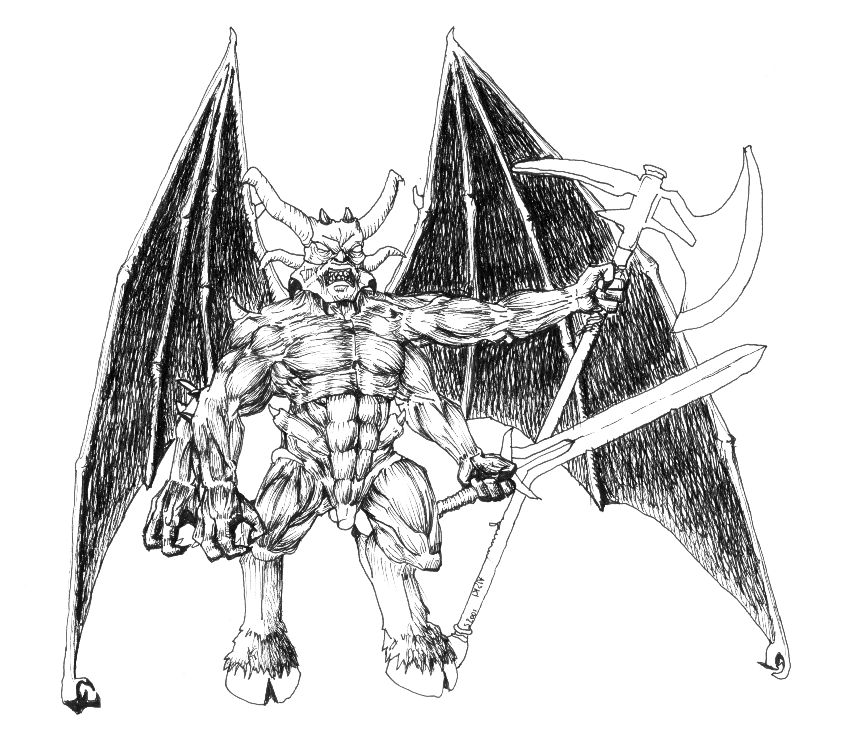
\includegraphics{arioch3.eps}
\end{center}
\end{figure*}

\demone{Arioch}{30}{Quinto Prisma}{Richiamabile} Appare come un grande
essere umanoide alto fino a 3 metri e mezzo. Appare nudo tranne che
per i foderi delle armi che porta con s\'e.

Ha quattro braccia con mani artigliate ed enormi ali membranose, che
possono raggiungere i 20 metri di apertura, terminanti con tre dita
artigliate.

Utilizza armi giganti solitamente ad una mano. Con le dita delle ali
pu\`o impugnare armi normali.


Ad una prima occhiata sembrerebbe avere la pelle rossa, in realt\`a
essa \`e assente; le fibre muscolari e i nervi sono direttamente
esposti all'aria, causandogli costantemente un atroce dolore di cui
Arioch gode.


Il suo volto appare costantemente animato da un'espressione mista di
dolore e piacere. I suoi occhi sono rossi e privi di pupille.  Il capo
\`e ornato da corna, sempre in numero pari e disposte
simmetricamente.

Arioch combatte utilizzando 2 Spade Bastarde giganti e 2 Alabarde
giganti. Talvolta abbandona le armi e combatte CAC utilizzando gli
artigli in grado di infliggere 2d8 PV/\-PSC di Danno; ama strappare
gli arti alle vittime e infilzarle sulle sue corna capaci di arrecare
2d8 PV/\-PSC di danno.

I suoi muscoli esposti all'aria sono comunque particolarmente
coriacei, tali da difenderlo come fossero una corazza di piastre (10
PP).

\carmostro{19+1d6}{15+1d10}{20+2d6}{20+1d10}{25+1d10}{25+1d8}{-1d10}{270}

\begin{parmostro}{Abilit\`a di Combattimento/TOT/Danno}
%%
\item CAC/AGI/2d8 
\item ATL/AGI/3d8+2 
\item ABL/AGI/3d8+1
\item AIA/AGI/3d8+1
\end{parmostro}

\begin{parmostro}{Attacchi Particolari/TOT/Danno}
%%
\item Corna/AGI/2d8
\end{parmostro}

\begin{parmostro}{Maestrie/TOT} 
%%
\item Spada Bastarda/AGI 
\item Alabarda/AGI
\end{parmostro}

\begin{parmostro}{Specifiche di AM/TOT/BON} 
%%
\item Presa/AGI/BON AGI
\end{parmostro}

\begin{parmostro}{Tecniche Speciali/TOT/BON} 
%%
\item Carica/20/+5
\end{parmostro}

\begin{parmostro}{Difese}
%%
\item Muscoli (PP 10)
\end{parmostro}

\begin{parmostro}{Poteri Speciali}
%%
\item Anima Diabolica
\item Fiamma Demoniaca
\item Schermo dell'Oblio
\item 13 Poteri a scelta del Master, con DR massima pari a 45.
\end{parmostro}

\demone{Belzeb\`u}{$\>$ 30}{Sesto Prisma}{Non Richiamabile} Appare
come una linea nera che disegna la sagoma di un umanoide alto sino a 2
m. Ha due sole dimensioni e qualora si volga di lato diventa
praticamente invisibile. Non lo si \`e mai sentito parlare e quando
intende comunicare disegna le parole nell'aria con la stessa linea che
delimita il suo corpo. Null'altro ci \`e dato sapere.

\demone{Baal}{$\>$ 30}{Settimo Prisma}{Non Richiamabile} Appare come un
giovane imberbe pallido e d'aspetto esile. Indossa esclusivamente un
perizoma. Il volto \`e contornato da lunghi riccioli neri e mostra
occhi chiarissimi; dal suo capo spuntano due piccole corna rivolte in
avanti. La sua voce sembra un sussurro. Si muove in maniera lenta e
indolente e sembra sempre afflitto da un profondo sentimento di
tristezza. Nessuno \`e sopravvissuto per fornire altre informazioni
su di lui.

\demone{Lo Dimonio}{$\>$ 30}{Ottavo Prisma}{Non Richiamabile}

La sua forma originaria \`e quella di un umano di etnia indefinita,
alto circa 180 cm, dalla carnagione olivastra.

Ha capelli neri portati lunghi o raccolti in una coda.  I suoi occhi
sono completamente neri.

La sua espressione \`e solitamente allegra e mostra un sorriso
malizioso. Dal capo spuntano due piccole corna nere che solitamente
nasconde fra i capelli. \`E solito abbigliarsi con vestiti lussuosi.
Porta sempre con s\'e un flauto di legno d'ebano capace di soggiogare
gli ascoltatori.

Pu\`o far nascere dalla sua schiena delle ali da rapace di colore
bianco atte al volo e la cui apertura raggiunge i 3.5 metri

\`E in grado di assumere le sembianze di qualsiasi altro demone. 

\subsubsection{I Demoni Generici}
\label{demonigenerici}

I demoni generici (introdotti a pagina \pageref{incantesimidemoni}) hanno le
forme pi\`u disparate. Solitamente, qualunque sia la forma base, vengono
estremizzate le caratteristiche proprie del demone specifico. 

\pinup{demonecorazza.eps}{Un demone generico (Corazza)}

Un demone che permette di udire avr\`a enormi orecchie, un demone
utile al trasporto avr\`a arti possenti, ecc.

\begin{description}
\item{\textbf{Potenza.}} la potenza \`e \textbf{pari alla DR}
  dell'incantesimo che manifesta il potere del demone.
  
\item{\textbf{Caratteristiche.}} Ognuna delle caratteristiche
  (BELlezza e CARisma escluse, determinate arbitrariamente dal Master)
  \`e pari a \textbf{1/2 della Potenza + 1d6}.
  
\item{\textbf{Energia.}} I PE utilizzabili per i poteri sono pari a
  \textbf{6 volte la Potenza}.
  
\item{\textbf{Poteri speciali.}}  Oltre al potere che si manifesta
  nell'incantesimo, i generici hanno un numero di poteri aggiuntivi a
  discrezione del Master pari ad \textbf{1/6 della Potenza}, ciascuno dei quali
  ha una \textbf{DR inferiore} alla Potenza.
  
\item{\textbf{Abilit\`a di Combattimento.}} I generici hanno un TOT nell'Abilit\`a
    \textbf{CAC pari ad AGI-3}.
\end{description}

\es{Gunnar vuole richiamare il Demone del
Gioco. L'incantesimo, che conferisce +5 all'abilit\`a Barare, ha DR 24. La
potenza del demone \`e 24; la DR dell'incantesimo che richiama uno di questi
demoni \`e 24 cio\`e 18 (DT) + 2 (Modificatori) + 24 (DB) - 20 (Modificatori)
= 24. Gunnar traccia il pentacolo e richiama il demone. Compare un essere umanoide
con la testa a forma di dado, le mani lunghissime e vestito di una tunica con
le maniche larghissime. Quest'essere, in base alla regola, avr\`a un VAL
alle caratteristiche pari a 24/2+1d6 cio\`e 12+1d6. 
 
Il Master tira i d6 ottenendo:
\begin{tabular}{ll}
  INT& 12 + 3 \\
  CONC& 12 + 5\\
  COS& 12 + 1\\ 
  AGI& 12 + 2 \\
  FOR& 12 + 5 \\ 
  OSS& 12 + 6 \\
\end{tabular}

Il demone avr\`a inoltre 144 PE, 4 poteri speciali aggiuntivi con DR
massima di 23 e un TOT in CAC pari a 14 (AGI)-3=11.

Il Master decide che i 4 poteri speciali aggiuntivi, oltre a Demone
del Gioco, del demone, sono: Acido, Corazza Infernale, Boccaglio e
Freccia Demoniaca}

\subsection{Gli Incantesimi}
\label{incdemonologia}
%----------------------------------------------------------------------------
\begin{spell}{Acido (Arkyox)}{Demonologia}{Attacco}{Danno Mirato}
%----------------------------------------------------------------------------
\descrizione{Dal mago parte uno spruzzo di acido che infligge ad un target a massimo 4 metri di distanza 1d6 PV/PSC di danno con base al TPC di 10.}
%% DR DA DT DB MOD PM PF PE TL
\incvalori{7}{23}{5}{15}{3}{7}{2}{23}{1}
\parametro{Danno}{1}{d6}{5}
\parametro{Base TPC}{10}{}{10}
\fineparametri
\gittata{4}{1}
\campo{1}{target}{2}
\durata{3 min}{0}
\end{spell}
%----------------------------------------------------------------------------
\begin{spell}{Ammorbidente (Rimmom)}{Demonologia}{Alterazione}{Variazione propriet\`a fisiche}
%----------------------------------------------------------------------------
\descrizione{Rende gli oggetti posti in un'area con un raggio di 4 metri, a distanza di massimo 10 metri dal mago, morbidi e inadatti a sorreggere pesi o a resistere agli urti. Il demone compare sotto forma di uno sciame di zanzare che succhiano materia dagli oggetti.}
%% DR DA DT DB MOD PM PF PE TL
\incvalori{31}{36}{15}{14}{7}{31}{10}{36}{5}
\parametro{Complessit\`a}{10}{}{10}
\parametro{Massa vivente}{100}{kg}{4}
\parametro{Massa non vivente}{0}{kg}{0}
\fineparametri
\gittata{10}{3}
\campo{4}{m}{4}
\durata{3 min}{0}
\end{spell}
%----------------------------------------------------------------------------
\begin{spell}{Anima diabolica (Foran)}{Demonologia}{Alterazione}{Creazione Esseri Viventi}
%----------------------------------------------------------------------------
\descrizione{Anima un oggetto (un monile, un'arma etc..) di 90 kg di peso massimo. L'incantesimo attribuisce 10 ad ogni caratteristica. L'oggetto si anima in 1d6 giorni.}
%% DR DA DT DB MOD PM PF PE TL
\incvalori{45}{50}{29}{23}{-2}{45}{15}{50}{7}
\parametro{Massa vivente}{90}{kg}{3}
\parametro{punti CAraTteristica}{80}{punti}{20}
\fineparametri
\gittatanulla
\campo{1}{target}{2}
\duratanulla
\azionetempo{1d6 giorni}{-3}
\end{spell}
%----------------------------------------------------------------------------
\begin{spell}{Aura demoniaca (Roneues)}{Demonologia}{Difesa}{Antimagia}
%----------------------------------------------------------------------------
\descrizione{Riveste il target di un'aura demoniaca rossastra che rende inattivo per 3 minuti qualsiasi incantesimo diretto al target con una base Antimagia di 20.}
%% DR DA DT DB MOD PM PF PE TL
\incvalori{22}{36}{15}{20}{1}{22}{7}{36}{3}
\parametro{Base antimagia}{20}{punti}{20}
\fineparametri
\gittatanulla
\campo{1}{target}{2}
\durata{3 min}{0}
\end{spell}
%----------------------------------------------------------------------------
\begin{spell}{Boccaglio (Gredlur)}{Demonologia}{Alterazione}{Modifica Anatomia per nuove funzioni}
%----------------------------------------------------------------------------
\descrizione{Un demone dalla forma di tubo telescopico (fino a 1 metro e 1/2) si collega con la bocca e il naso del target consentendogli di respirare sott'acqua o sotto terra. Il demone scompare dopo 3 minuti.}
%% DR DA DT DB MOD PM PF PE TL
\incvalori{22}{27}{15}{11}{1}{22}{7}{27}{3}
\parametro{Complessit\`a}{10}{}{10}
\parametro{Massa vivente}{5}{kg}{1}
\parametro{Fattore dimensione}{0}{unit\`a}{0}
\fineparametri
\gittatanulla
\campo{1}{target}{2}
\durata{3 min}{0}
\end{spell}
%----------------------------------------------------------------------------
\begin{spell}{Colonna di fuoco (Ighnar)}{Demonologia}{Attacco}{Danno Netto}
%----------------------------------------------------------------------------
\descrizione{Emette una fiammata che si propaga dal basso verso l'alto e che provoca 4d6 PV di danno su un'area di 2 metri di raggio situata fino a 10 metri dal mago. I danni possono essere dimezzati realizzando un TR a Diff. 18.}
%% DR DA DT DB MOD PM PF PE TL
\incvalori{18}{34}{21}{8}{5}{18}{6}{34}{3}
\parametro{Danno}{4}{d6}{8}
\fineparametri
\gittata{10}{3}
\campo{2}{m}{2}
\duratanulla
\end{spell}
%----------------------------------------------------------------------------
\begin{spell}{Corazza infernale (Reshpus)}{Demonologia}{Difesa}{Armatura}
%----------------------------------------------------------------------------
\descrizione{Un demone umanoide dal corpo cavo avvolge il corpo del target fornendogli 5 PP su tutto il corpo per 3 minuti.}
%% DR DA DT DB MOD PM PF PE TL
\incvalori{16}{30}{19}{10}{1}{16}{5}{30}{2}
\parametro{Protezione}{5}{PP}{10}
\fineparametri
\gittatanulla
\campo{1}{target}{2}
\durata{3 min}{0}
\end{spell}
%----------------------------------------------------------------------------
\begin{spell}{Decuria di Mammon}{Demonologia}{Evocazione}{Richiamo}
%----------------------------------------------------------------------------
\descrizione{Il mago evoca 10 demoni guerrieri Mammon. Il TV per il controllo viene effettuato separatamente da ciascuno di essi.}
%% DR DA DT DB MOD PM PF PE TL
\incvalori{22}{42}{18}{4}{20}{22}{7}{42}{3}
\parametro{Potenza della creatura}{4}{}{4}
\fineparametri
\gittata{1}{0}
\campo{10}{target}{20}
\durata{3 min}{0}
\end{spell}
%----------------------------------------------------------------------------
\begin{spell}{Demone del gioco (Abolam)}{Demonologia}{Alterazione}{Variazione abilit\`a fisica}
%----------------------------------------------------------------------------
\descrizione{Conferisce al target un bonus di +5 all'abilit\`a Barare per la durata della concentrazione del mago + 3 minuti.}
%% DR DA DT DB MOD PM PF PE TL
\incvalori{24}{29}{18}{5}{6}{24}{8}{29}{4}
\parametro{Variazione abilit\`a}{5}{punti}{5}
\fineparametri
\gittatanulla
\campo{1}{target}{2}
\durata{concentrazione+3 min}{5+0}
\end{spell}
%----------------------------------------------------------------------------
\begin{spell}{Difensore (Pazooso)}{Demonologia}{Difesa}{Protezione Magica}
%----------------------------------------------------------------------------
\descrizione{Il target viene protetto dal demone difensore che si manifesta come uno sciame di insetti vorticante che gli assorbe 4d6 PV di danno provocato dagli incantesimi di Attacco/Danno Netto. L'incantesimo ha durata 3 minuti.}
%% DR DA DT DB MOD PM PF PE TL
\incvalori{15}{29}{20}{8}{1}{15}{5}{29}{2}
\parametro{Protezione}{4}{d6}{8}
\fineparametri
\gittatanulla
\campo{1}{target}{2}
\durata{3 min}{0}
\end{spell}
%----------------------------------------------------------------------------
\begin{spell}{Doppelganger (Hutgin)}{Demonologia}{Controllo}{Miraggio completo}
%----------------------------------------------------------------------------
\descrizione{Un demone assume le sembianze del mago e si rende visibile ad una distanza di massimo 7 metri dal mago stesso senza peraltro potersi muovere al di fuori di un'area di 2 metri di raggio. Realizzando un TOSS a Diff. 20 ci si rende conto che si tratta di una copia, che sparisce se si realizza un TV a Diff. 20. La copia non pu\`o combattere. L'incantesimo dura 15 minuti.}
%% DR DA DT DB MOD PM PF PE TL
\incvalori{26}{36}{9}{20}{7}{26}{8}{36}{4}
\parametro{Difficolt\`a del TV e del TOSS}{20}{}{20}
\fineparametri
\gittata{7}{2}
\campo{2}{m}{2}
\durata{15 min}{3}
\end{spell}
%----------------------------------------------------------------------------
\begin{spell}{Evoca Alastor}{Demonologia}{Evocazione}{Richiamo}
%----------------------------------------------------------------------------
\descrizione{Evoca il demone guerriero Alastor per 3 minuti. Il mago pu\`o impartirgli ordini se vince un confronto di TV con esso.}
%% DR DA DT DB MOD PM PF PE TL
\incvalori{14}{34}{18}{14}{2}{14}{4}{34}{2}
\parametro{Potenza della creatura}{14}{}{14}
\fineparametri
\gittata{1}{0}
\campo{1}{target}{2}
\durata{3 min}{0}
\end{spell}
%----------------------------------------------------------------------------
\begin{spell}{Evoca Ammon}{Demonologia}{Evocazione}{Richiamo}
%----------------------------------------------------------------------------
\descrizione{Evoca il demone guerriero Ammon per 3 minuti. Il mago pu\`o impartirgli ordini se vince un confronto di TV con esso.}
%% DR DA DT DB MOD PM PF PE TL
\incvalori{9}{29}{18}{9}{2}{9}{3}{29}{1}
\parametro{Potenza della creatura}{9}{}{9}
\fineparametri
\gittata{1}{0}
\campo{1}{target}{2}
\durata{3 min}{0}
\end{spell}
%----------------------------------------------------------------------------
\begin{spell}{Evoca Arioch}{Demonologia}{Evocazione}{Richiamo}
%----------------------------------------------------------------------------
\descrizione{Evoca il demone guerriero Arioch per 3 minuti. Il mago pu\`o impartirgli ordini se vince un confronto di TV con esso.}
%% DR DA DT DB MOD PM PF PE TL
\incvalori{30}{50}{18}{30}{2}{30}{10}{50}{5}
\parametro{Potenza della creatura}{30}{}{30}
\fineparametri
\gittata{1}{0}
\campo{1}{target}{2}
\durata{3 min}{0}
\end{spell}
%----------------------------------------------------------------------------
\begin{spell}{Evoca Mammon}{Demonologia}{Evocazione}{Richiamo}
%----------------------------------------------------------------------------
\descrizione{Evoca il demone guerriero Mammon per 3 minuti. Il mago pu\`o impartirgli ordini se vince un confronto di TV con esso.}
%% DR DA DT DB MOD PM PF PE TL
\incvalori{4}{24}{18}{4}{2}{4}{1}{24}{1}
\parametro{Potenza della creatura}{4}{}{4}
\fineparametri
\gittata{1}{0}
\campo{1}{target}{2}
\durata{3 min}{0}
\end{spell}
%----------------------------------------------------------------------------
\begin{spell}{Evoca Strayesor}{Demonologia}{Evocazione}{Richiamo}
%----------------------------------------------------------------------------
\descrizione{Evoca il demone guerriero Strayesor per 3 minuti. Il mago pu\`o impartirgli ordini se vince un confronto di TV con esso.}
%% DR DA DT DB MOD PM PF PE TL
\incvalori{19}{39}{18}{19}{2}{19}{6}{39}{3}
\parametro{Potenza della creatura}{19}{}{19}
\fineparametri
\gittata{1}{0}
\campo{1}{target}{2}
\durata{3 min}{0}
\end{spell}
%----------------------------------------------------------------------------
\begin{spell}{Fascino satanico (Kham)}{Demonologia}{Controllo}{Comando}
%----------------------------------------------------------------------------
\descrizione{Gli esseri situati all'interno di un'area di un metro di raggio che non realizzano un TV a Diff. 20 vengono affascinati irresistibilmente dal mago per 3 minuti.}
%% DR DA DT DB MOD PM PF PE TL
\incvalori{22}{32}{11}{20}{1}{22}{7}{32}{3}
\parametro{Difficolt\`a del TV}{20}{}{20}
\fineparametri
\gittata{1}{0}
\campo{1}{m}{1}
\durata{3 min}{0}
\end{spell}
%----------------------------------------------------------------------------
\begin{spell}{Fiamma demoniaca (Rahouart)}{Demonologia}{Attacco}{Danno Netto}
%----------------------------------------------------------------------------
\descrizione{Fa partire dal mago una fiammata larga 20 metri che distrugge tutto ci\`o su cui passa, per una gittata di massimo 19 metri, esplodendo poi su un'area di 10 metri di raggio e provocando a tutti gli oggetti investiti un danno di 10d6 PV. Le vittime possono dimezzare il danno realizzando un TR a Diff. 30. La fiamma pu\`o produrre danni addizionali.}
%% DR DA DT DB MOD PM PF PE TL
\incvalori{44}{60}{21}{20}{19}{44}{14}{60}{7}
\parametro{Danno}{10}{d6}{20}
\fineparametri
\gittata{19}{6}
\azionegittata
\campo{10}{m}{10}
\duratanulla
\end{spell}
%----------------------------------------------------------------------------
\begin{spell}{Filamento adesivo (Poimon)}{Demonologia}{Difesa}{Parata}
%----------------------------------------------------------------------------
\descrizione{Dal corpo del target si diparte un filamento adesivo atto a parare un colpo con Base TPD 5. Dopo 3 minuti o dopo una parata il filamento scompare.}
%% DR DA DT DB MOD PM PF PE TL
\incvalori{9}{23}{15}{7}{1}{9}{3}{23}{1}
\parametro{Base TPD}{5}{punti}{5}
\parametro{Parate}{1}{}{2}
\fineparametri
\gittatanulla
\campo{1}{target}{2}
\durata{3 min}{0}
\end{spell}
%----------------------------------------------------------------------------
\begin{spell}{Freccia demoniaca (Dreayn)}{Demonologia}{Attacco}{Danno Mirato}
%----------------------------------------------------------------------------
\descrizione{Fa scaturire dal mago un piccolo demone simile ad una larva dotata di zanne che si scaglia sul target, distante massimo 10 metri, mordendolo e infliggendogli 1d6 PV/PSC di danno. La base TPC \`e 15.}
%% DR DA DT DB MOD PM PF PE TL
\incvalori{14}{30}{5}{20}{5}{14}{4}{30}{2}
\parametro{Danno}{1}{d6}{5}
\parametro{Base TPC}{15}{}{15}
\fineparametri
\gittata{10}{3}
\campo{1}{target}{2}
\duratanulla
\end{spell}
%----------------------------------------------------------------------------
\begin{spell}{Globo demoniaco (Kira)}{Demonologia}{Difesa}{Antimagia}
%----------------------------------------------------------------------------
\descrizione{Crea un globo di luce demoniaca rossastra di 1 metro di raggio per 3 minuti. Qualunque incantesimo diretto ad esseri od oggetti all'interno del globo sar\`a neutralizzato con una base antimagia di 20. Il mago pu\`o creare il globo fino a 1 metro di distanza da s\'e.}
%% DR DA DT DB MOD PM PF PE TL
\incvalori{22}{36}{15}{20}{1}{22}{7}{36}{3}
\parametro{Base antimagia}{20}{punti}{20}
\fineparametri
\gittata{1}{0}
\campo{1}{m}{1}
\durata{3 min}{0}
\end{spell}
%----------------------------------------------------------------------------
\begin{spell}{Guanto (Adramelek)}{Demonologia}{Attacco}{Morte}
%----------------------------------------------------------------------------
\descrizione{Il target che non realizza un TR a Diff. 20 viene rivoltato come un guanto, morendo istantaneamente. Il corpo torna intatto dopo un incantesimo di resurrezione.}
%% DR DA DT DB MOD PM PF PE TL
\incvalori{23}{39}{18}{20}{1}{23}{7}{39}{3}
\parametro{Difficolt\`a del TR}{20}{}{20}
\fineparametri
\gittatanulla
\campo{1}{target}{2}
\duratanulla
\end{spell}
%----------------------------------------------------------------------------
\begin{spell}{Guaritore (Baribars)}{Demonologia}{Difesa}{Cura}
%----------------------------------------------------------------------------
\descrizione{Con questo incantesimo, il mago \`e in grado, grazie al demone Guaritore, di curare 3d6 PV/PSC di danno a tutti gli esseri viventi posti ad una distanza massima di 1 metro da lui ed in un'area di 1 metro di raggio. L'incantesimo lascia tracce visibili della cura sotto forma di  escrescenze cutanee o simili.}
%% DR DA DT DB MOD PM PF PE TL
\incvalori{14}{28}{21}{6}{1}{14}{4}{28}{2}
\parametro{Riparazione}{3}{d6}{6}
\fineparametri
\gittata{1}{0}
\campo{1}{m}{1}
\duratanulla
\end{spell}
%----------------------------------------------------------------------------
\begin{spell}{Individua demoni (Zebuliel)}{Demonologia}{Informazione}{Divinazione}
%----------------------------------------------------------------------------
\descrizione{L'incantesimo individua la presenza di uno o pi\`u demoni nel raggio di 10 metri, senza indicarne la collocazione.}
%% DR DA DT DB MOD PM PF PE TL
\incvalori{18}{28}{9}{10}{9}{18}{6}{28}{3}
\parametro{DIFF reperimento informazione}{10}{}{10}
\parametro{Previsione}{0}{ore}{0}
\fineparametri
\gittatanulla
\campo{10}{m}{10}
\durata{3 min}{0}
\end{spell}
%----------------------------------------------------------------------------
\begin{spell}{Intercettatore (Zyunsak)}{Demonologia}{Difesa}{Parata}
%----------------------------------------------------------------------------
\descrizione{Il target viene protetto dal Demone intercettatore in grado di parare 5 attacchi fisici o di Attacco/Danno Mirato con una base di parata di 15. Il demone svanisce dopo 3 minuti oppure dopo aver parato 5 attacchi.}
%% DR DA DT DB MOD PM PF PE TL
\incvalori{27}{41}{15}{25}{1}{27}{9}{41}{4}
\parametro{Base TPD}{15}{punti}{15}
\parametro{Parate}{5}{}{10}
\fineparametri
\gittatanulla
\campo{1}{target}{2}
\durata{3 min}{0}
\end{spell}
%----------------------------------------------------------------------------
\begin{spell}{Macellaio (Greayn)}{Demonologia}{Attacco}{Danno Mirato}
%----------------------------------------------------------------------------
\descrizione{La vittima viene scuoiata nel punto di contatto con la mano dell'usufruitore, ricevendo 3d6 PV/PSC di danno. Infligge danni addizionali da emorragia. L'usufruitore potrebbe dover realizzare un TPC con l'abilit\`a CAC.}
%% DR DA DT DB MOD PM PF PE TL
\incvalori{5}{21}{5}{15}{1}{5}{1}{21}{1}
\parametro{Danno}{3}{d6}{15}
\parametro{Base TPC}{0}{}{0}
\fineparametri
\gittatanulla
\campo{1}{target}{2}
\durata{3 min}{0}
\end{spell}
%----------------------------------------------------------------------------
\begin{spell}{Mantici (Iblis)}{Demonologia}{Alterazione}{Spostamento 3 dimensioni}
%----------------------------------------------------------------------------
\descrizione{Alcuni piccoli demoni che ingoiano ed emettono aria si attaccano al corpo del target del peso massimo di 90 kg e con un equipaggiamento di massimo 100 kg, consentendogli di volare per 3 minuti a 100 km/h.}
%% DR DA DT DB MOD PM PF PE TL
\incvalori{29}{34}{19}{14}{1}{29}{9}{34}{4}
\parametro{Massa vivente}{90}{kg}{3}
\parametro{Velocit\`a}{100}{km/h}{10}
\parametro{Massa non vivente}{90}{kg}{1}
\fineparametri
\gittatanulla
\campo{1}{target}{2}
\durata{3 min}{0}
\end{spell}
%----------------------------------------------------------------------------
\begin{spell}{Messaggero (Belialys)}{Demonologia}{Informazione}{Trasmissione+Ricezione}
%----------------------------------------------------------------------------
\descrizione{Un demone messaggero recapita istantaneamente un messaggio scritto di poche pagine ad un target posto ad una distanza massima di 10 km, ricevendo una eventuale risposta e riportandola al mago.}
%% DR DA DT DB MOD PM PF PE TL
\incvalori{26}{36}{15}{20}{1}{26}{8}{36}{4}
\parametro{Complessit\`a}{4}{}{4}
\parametro{Distanza}{10000}{m}{16}
\fineparametri
\gittatanulla
\campo{1}{target}{2}
\duratanulla
\end{spell}
%----------------------------------------------------------------------------
\begin{spell}{Patto Demoniaco (Haflain)}{Demonologia}{Controllo}{Comando}
%----------------------------------------------------------------------------
\descrizione{Con questo incantesimo il mago pu\`o, grazie al demone persuasore, obbligare tutti coloro che si trovano alla distanza massima di 1 metro e nell'area di 1 metro di raggio, ad eseguire un ordine a suo piacimento, se questi non realizzano un TV a Diff. 20. Per tutte le vittime l'ordine \`e lo stesso.}
%% DR DA DT DB MOD PM PF PE TL
\incvalori{22}{32}{11}{20}{1}{22}{7}{32}{3}
\parametro{Difficolt\`a del TV}{20}{}{20}
\fineparametri
\gittata{1}{0}
\campo{1}{m}{1}
\durata{3 min}{0}
\end{spell}
%----------------------------------------------------------------------------
\begin{spell}{Pelle robusta (Tsu Nyao)}{Demonologia}{Difesa}{Armatura}
%----------------------------------------------------------------------------
\descrizione{La pelle del target si ingrossa e si ricopre di escrescenze cornee che la rendono dura e dotata di 1 PP, per 7 minuti.}
%% DR DA DT DB MOD PM PF PE TL
\incvalori{9}{23}{19}{2}{2}{9}{3}{23}{1}
\parametro{Protezione}{1}{PP}{2}
\fineparametri
\gittatanulla
\campo{1}{target}{2}
\durata{7 min}{1}
\end{spell}
%----------------------------------------------------------------------------
\begin{spell}{Pelle viscida (Abludar)}{Demonologia}{Alterazione}{Variazione abilit\`a fisica}
%----------------------------------------------------------------------------
\descrizione{Il target viene rivestito da uno strato di liquido viscoso e scivoloso che gli conferisce un bonus di +5 al TOT della Specifica di AM ``divincolarsi''.}
%% DR DA DT DB MOD PM PF PE TL
\incvalori{19}{24}{18}{5}{1}{19}{6}{24}{3}
\parametro{Variazione abilit\`a}{5}{punti}{5}
\fineparametri
\gittatanulla
\campo{1}{target}{2}
\durata{3 min}{0}
\end{spell}
%----------------------------------------------------------------------------
\begin{spell}{Portatore di dolore (Koim)}{Demonologia}{Informazione}{Variazione abilit\`a mentale}
%----------------------------------------------------------------------------
\descrizione{Il demone conferisce al target un bonus di +5 all'abilit\`a Torture per 15 minuti.}
%% DR DA DT DB MOD PM PF PE TL
\incvalori{17}{27}{18}{5}{4}{17}{5}{27}{2}
\parametro{Variazione abilit\`a}{5}{punti}{5}
\fineparametri
\gittatanulla
\campo{1}{target}{2}
\durata{15 min}{3}
\end{spell}
%----------------------------------------------------------------------------
\begin{spell}{Possesso diabolico (Behemoth)}{Demonologia}{Controllo}{Possessione}
%----------------------------------------------------------------------------
\descrizione{L'usufruitore si impossessa del corpo di un target per 3 minuti, se questi non realizza un TV a Diff. 20.}
%% DR DA DT DB MOD PM PF PE TL
\incvalori{22}{32}{11}{20}{1}{22}{7}{32}{3}
\parametro{Difficolt\`a del TV}{20}{}{20}
\fineparametri
\gittatanulla
\campo{1}{target}{2}
\durata{3 min}{0}
\end{spell}
%----------------------------------------------------------------------------
\begin{spell}{Protezione dai Demoni I}{Demonologia}{Evocazione}{Protezione}
%----------------------------------------------------------------------------
\descrizione{Viene creata, attorno ad un punto distante al massimo 4 metri dal mago, un'area di 3 metri di raggio all'interno della quale i Demoni di potenza uguale o inferiore a 9 non possono entrare se non realizzando un TV a Diff. 19. Realizzando il TV le creature potranno avanzare di 1 metro, subendo 1d6 PV di danno per ogni metro all'interno dell'area, L'incantesimo scompare se il mago attacca le creature dalle quali si sta proteggendo. Per ogni metro all'interno dell'area il TV delle creature \`e penalizzato di -1. L'incantesimo perdura per 3 minuti.}
%% DR DA DT DB MOD PM PF PE TL
\incvalori{3}{23}{10}{9}{4}{3}{1}{23}{1}
\parametro{Potenza della creatura}{9}{}{9}
\fineparametri
\gittata{4}{1}
\campo{3}{m}{3}
\durata{3 min}{0}
\end{spell}
%----------------------------------------------------------------------------
\begin{spell}{Protezione dai Demoni II}{Demonologia}{Evocazione}{Protezione}
%----------------------------------------------------------------------------
\descrizione{Viene creata, attorno ad un punto distante al massimo 4 metri dal mago, un'area di 3 metri di raggio all'interno della quale i Demoni di potenza uguale o inferiore a 19 non possono entrare se non realizzando un TV a Diff. 29. Realizzando il TV le creature potranno avanzare di 1 metro, subendo 1d6 PV di danno per ogni metro all'interno dell'area, L'incantesimo scompare se il mago attacca le creature dalle quali si sta proteggendo. Per ogni metro all'interno dell'area il TV delle creature \`e penalizzato di -1. L'incantesimo perdura per 3 minuti.}
%% DR DA DT DB MOD PM PF PE TL
\incvalori{13}{33}{10}{19}{4}{13}{4}{33}{2}
\parametro{Potenza della creatura}{19}{}{19}
\fineparametri
\gittata{4}{1}
\campo{3}{m}{3}
\durata{3 min}{0}
\end{spell}
%----------------------------------------------------------------------------
\begin{spell}{Protezione dai Demoni III}{Demonologia}{Evocazione}{Protezione}
%----------------------------------------------------------------------------
\descrizione{Viene creata, attorno ad un punto distante al massimo 4 metri dal mago, un'area di 3 metri di raggio all'interno della quale i Demoni di potenza uguale o inferiore a 30 non possono entrare se non realizzando un TV a Diff. 40. Realizzando il TV le creature potranno avanzare di 1 metro, subendo 1d6 PV di danno per ogni metro all'interno dell'area, L'incantesimo scompare se il mago attacca le creature dalle quali si sta proteggendo. Per ogni metro all'interno dell'area il TV delle creature \`e penalizzato di -1. L'incantesimo perdura per 3 minuti.}
%% DR DA DT DB MOD PM PF PE TL
\incvalori{24}{44}{10}{30}{4}{24}{8}{44}{4}
\parametro{Potenza della creatura}{30}{}{30}
\fineparametri
\gittata{4}{1}
\campo{3}{m}{3}
\durata{3 min}{0}
\end{spell}
%----------------------------------------------------------------------------
\begin{spell}{Rostro (Morkooya)}{Demonologia}{Alterazione}{Modifica Danni anatomia/armi}
%----------------------------------------------------------------------------
\descrizione{Il braccio del target viene rivestito da una superficie dura, rugosa e dotata di punte acuminate, rendendo il danno base di Pugno pari a 1d4 + 2d6. L'incantesimo dura 3 minuti.}
%% DR DA DT DB MOD PM PF PE TL
\incvalori{27}{32}{20}{11}{1}{27}{9}{32}{4}
\parametro{Danno}{2}{d6}{10}
\parametro{Massa}{5}{kg}{1}
\fineparametri
\gittatanulla
\campo{1}{target}{2}
\durata{3 min}{0}
\end{spell}
%----------------------------------------------------------------------------
\begin{spell}{Schermo dell'Oblio (Krisral)}{Demonologia}{Difesa}{Deviazione}
%----------------------------------------------------------------------------
\descrizione{Il target viene protetto da uno schermo che para tutti gli attacchi fisici o di Attacco/Danno Mirato con base TPD 20. L'incantesimo dura 3 minuti.}
%% DR DA DT DB MOD PM PF PE TL
\incvalori{32}{46}{25}{20}{1}{32}{10}{46}{5}
\parametro{Base TPD}{20}{punti}{20}
\fineparametri
\gittatanulla
\campo{1}{target}{2}
\durata{3 min}{0}
\end{spell}
%----------------------------------------------------------------------------
\begin{spell}{Seduttore (Azazel)}{Demonologia}{Alterazione}{Variazione abilit\`a fisica}
%----------------------------------------------------------------------------
\descrizione{Conferisce al target un bonus di +5 all'abilit\`a Sedurre per 15 minuti.}
%% DR DA DT DB MOD PM PF PE TL
\incvalori{22}{27}{18}{5}{4}{22}{7}{27}{3}
\parametro{Variazione abilit\`a}{5}{punti}{5}
\fineparametri
\gittatanulla
\campo{1}{target}{2}
\durata{15 min}{3}
\end{spell}
%----------------------------------------------------------------------------
\begin{spell}{Sguardo di fuoco (Ayperos)}{Demonologia}{Alterazione}{Modifica Anatomia per nuove funzioni}
%----------------------------------------------------------------------------
\descrizione{Gli occhi del target saranno modificati in modo da vedere al buio. Gli occhi brilleranno di una sinistra luce rossastra. L'incantesimo dura a concentrazione pi\`u 3 minuti.}
%% DR DA DT DB MOD PM PF PE TL
\incvalori{22}{27}{15}{6}{6}{22}{7}{27}{3}
\parametro{Complessit\`a}{5}{}{5}
\parametro{Massa vivente}{1}{kg}{1}
\parametro{Fattore dimensione}{0}{unit\`a}{0}
\fineparametri
\gittatanulla
\campo{1}{target}{2}
\durata{concentrazione+3 min}{5+0}
\end{spell}
%----------------------------------------------------------------------------
\begin{spell}{Sottomissione Demoni I}{Demonologia}{Evocazione}{Controllo}
%----------------------------------------------------------------------------
\descrizione{Consente di sottomettere ai propri ordini un demone di potenza massima pari a 9 per 3 minuti. Il mago pu\`o impartirgli ordini se vince un confronto di TV con esso se \`e un essere errante, o con chi lo domina se \`e controllato..}
%% DR DA DT DB MOD PM PF PE TL
\incvalori{6}{26}{14}{9}{3}{6}{2}{26}{1}
\parametro{Potenza della creatura}{9}{}{9}
\fineparametri
\gittata{4}{1}
\campo{1}{target}{2}
\durata{3 min}{0}
\end{spell}
%----------------------------------------------------------------------------
\begin{spell}{Sottomissione Demoni II}{Demonologia}{Evocazione}{Controllo}
%----------------------------------------------------------------------------
\descrizione{Consente di sottomettere ai propri ordini un demone di potenza massima pari a 19 per 3 minuti. Il mago pu\`o impartirgli ordini se vince un confronto di TV con esso se \`e un essere errante, o con chi lo domina se \`e controllato..}
%% DR DA DT DB MOD PM PF PE TL
\incvalori{16}{36}{14}{19}{3}{16}{5}{36}{2}
\parametro{Potenza della creatura}{19}{}{19}
\fineparametri
\gittata{4}{1}
\campo{1}{target}{2}
\durata{3 min}{0}
\end{spell}
%----------------------------------------------------------------------------
\begin{spell}{Sottomissione Demoni III}{Demonologia}{Evocazione}{Controllo}
%----------------------------------------------------------------------------
\descrizione{Consente di sottomettere ai propri ordini un demone di potenza massima pari a 30 per 3 minuti. Il mago pu\`o impartirgli ordini se vince un confronto di TV con esso se \`e un essere errante, o con chi lo domina se \`e controllato..}
%% DR DA DT DB MOD PM PF PE TL
\incvalori{27}{47}{14}{30}{3}{27}{9}{47}{4}
\parametro{Potenza della creatura}{30}{}{30}
\fineparametri
\gittata{4}{1}
\campo{1}{target}{2}
\durata{3 min}{0}
\end{spell}
%----------------------------------------------------------------------------
\begin{spell}{Sparizione (Gusartan)}{Demonologia}{Alterazione}{Teletrasporto standard}
%----------------------------------------------------------------------------
\descrizione{Teletrasporta il target a 100 metri di distanza in un punto in cui il demonologo \`e gi\`a stato. Il target deve pesare al massimo 90 kg ed avere non pi\`u di 100 kg di equipaggiamento. Il target pu\`o subire danni a discrezione del Master se il punto di destinazione \`e inagibile o gi\`a occupato.}
%% DR DA DT DB MOD PM PF PE TL
\incvalori{29}{34}{19}{14}{1}{29}{9}{34}{4}
\parametro{Massa vivente}{90}{kg}{3}
\parametro{Massa non vivente}{100}{kg}{1}
\parametro{Distanza di spostamento}{100}{m}{10}
\fineparametri
\gittatanulla
\campo{1}{target}{2}
\duratanulla
\end{spell}
%----------------------------------------------------------------------------
\begin{spell}{Suggeritore (Wala)}{Demonologia}{Informazione}{Variazione CONoscenza}
%----------------------------------------------------------------------------
\descrizione{Il target rester\`a in contatto col demone suggeritore, facendo aumentare di +1 la caratteristica CON, per il tempo in cui il mago terr\`a la concentrazione pi\`u 3 minuti.}
%% DR DA DT DB MOD PM PF PE TL
\incvalori{21}{31}{19}{6}{6}{21}{7}{31}{3}
\parametro{Variazione caratteristica}{1}{punto}{6}
\fineparametri
\gittatanulla
\campo{1}{target}{2}
\durata{concentrazione+3 min}{5+0}
\end{spell}
%----------------------------------------------------------------------------
\begin{spell}{Tentacoli (Belfagor)}{Demonologia}{Difesa}{Scudo antidinamico}
%----------------------------------------------------------------------------
\descrizione{L'usufruitore viene ricoperto da piccolissimi tentacoli che gli permettono di dimezzare tutti i danni da botta, da punta e da taglio, compresi quelli prodotti dagli incantesimi di Attacco/Danno Mirato, che gli vengono inflitti.}
%% DR DA DT DB MOD PM PF PE TL
\incvalori{18}{32}{21}{10}{1}{18}{6}{32}{3}
\parametro{Divisore}{2}{unit\`a}{10}
\fineparametri
\gittatanulla
\campo{1}{target}{2}
\durata{3 min}{0}
\end{spell}
%----------------------------------------------------------------------------
\begin{spell}{Tentazione (Schax)}{Demonologia}{Controllo}{Illusione completa}
%----------------------------------------------------------------------------
\descrizione{Mostra alle vittime situate in un'area di 1 metro di raggio distante fino a 1 metro dal mago immagini suadenti e ammaliatrici, che verranno percepite anche con tatto, olfatto, udito. Un TOSS a Diff. 20 render\`a consapevoli le vittime che le immagini non sono reali. In seguito, un TV a Diff. 20 potr\`a farle scomparire.}
%% DR DA DT DB MOD PM PF PE TL
\incvalori{20}{30}{9}{20}{1}{20}{6}{30}{3}
\parametro{Difficolt\`a del TV e del TOSS}{20}{}{20}
\fineparametri
\gittata{1}{0}
\campo{1}{m}{1}
\durata{3 min}{0}
\end{spell}
%----------------------------------------------------------------------------
\begin{spell}{Tipografo (Pruslas)}{Demonologia}{Informazione}{Registrazione}
%----------------------------------------------------------------------------
\descrizione{Ricopia un breve libro su un mazzo di fogli bianchi o simili, aggiungendo disegni osceni o raccapriccianti alla copia. La copia termina in 1d6 ore ed \`e permanente. L'incantesimo non ricopia correttamente i libri magici.}
%% DR DA DT DB MOD PM PF PE TL
\incvalori{33}{43}{22}{5}{16}{33}{11}{43}{5}
\parametro{Complessit\`a}{5}{}{5}
\fineparametri
\gittatanulla
\campo{1}{target}{2}
\durata{permanente }{15}
\end{spell}
%----------------------------------------------------------------------------
\begin{spell}{Violinista (Shentsow)}{Demonologia}{Attacco}{Stordimento}
%----------------------------------------------------------------------------
\descrizione{Pizzica i nervi delle vittime che si trovano in un'area di 2 metri di raggio distante fino a 10 metri dal target come fossero corde di violino, causandone lo stordimento (inabilitazione per il round in corso e quello successivo).}
%% DR DA DT DB MOD PM PF PE TL
\incvalori{18}{34}{9}{20}{5}{18}{6}{34}{3}
\parametro{Difficolt\`a del TR}{20}{}{20}
\fineparametri
\gittata{10}{3}
\campo{2}{m}{2}
\duratanulla
\end{spell}
%----------------------------------------------------------------------------
\begin{spell}{Zanna di luce (Guang Ya)}{Demonologia}{Attacco}{Danno Mirato}
%----------------------------------------------------------------------------
\descrizione{Un demone dalla forma della testa di un serpente luminescente infligge 2d6 PV/PSC di danno ad un target che si trova a massimo 7 metri dal mago. Il TPC \`e pari a 12.}
%% DR DA DT DB MOD PM PF PE TL
\incvalori{15}{31}{5}{22}{4}{15}{5}{31}{2}
\parametro{Danno}{2}{d6}{10}
\parametro{Base TPC}{12}{}{12}
\fineparametri
\gittata{7}{2}
\campo{1}{target}{2}
\duratanulla
\end{spell}

\vfill
\fi
%%---------------------------------------------------------------------------
\section{Elementalismo} 
%%---------------------------------------------------------------------------
\Simbolo{simb_ele.eps}

Parte del regno Memath, l'Elementalismo, detta Via degli Elementi in
Elfico, o Magia della Materia in Novese, governa i quattro elementi
Aria, Fuoco, Acqua e Terra.

Simbolo degli elementalisti \`e un triangolo equilatero,
diviso in quattro bande orizzontali, con il vertice rivolto verso il
basso.

\subsection{Dominio} 

L'Elementalismo domina ed attinge il suo potere dall'essenza degli
elementi, ordinati gerarchicamente col seguente schema: Aria (base),
Fuoco, Acqua e Pietra (apice), in modo che siano potenzialmente pi\`u
forti gli elementi che per affinit\`a sono pi\`u vicini alla Terra.
L'aria, di per s\'e, \`e gi\`a al di sopra della Terra; il Fuoco ha
sempre contatti diretti col terreno, mentre l'acqua \`e di natura
pi\`u pesante dell'aria e tender\`a a restare a contatto con la terra.
Inoltre, provate a soffiare dell'aria in una polla d'acqua: essa
risalir\`a rapidamente per riunirsi all'aria che si trova sopra la
polla.

La Pietra conferisce il
potere maggiore in quanto elemento primario del Piano Materiale. 

Tutti
gli incantesimi di questa scuola devono essere correlati con almeno
uno dei quattro elementi.

\subsection{Limiti e peculiarit\`a} 

Gli usufruitori che conoscono questa scuola sono gli unici a poter
evocare le creature elementali, e solo queste. Si pu\`o evocare un
elementale solo se l'elemento da cui prende essenza esiste in grande
quantit\`a o predominanza nel luogo dell'evocazione. Non si possono
evocare gli elementali dell'aria in luoghi senza contatti con
l'esterno. Non si possono evocare elementali della pietra in mare, sui
laghi o sui corsi d'acqua, e tanto meno in aria. Gli elementali del
fuoco si possono chiamare soltanto in prossimit\`a di una fiamma
viva, delle dimensioni di almeno un focolare, gli elementali
dell'acqua solo in prossimit\`a di specchi o corsi d'acqua, o quando
piove.

\subsection{Potenzialit\`a}

\begin{tabular}{lc}
Evocazione&11\\
Alterazione& 16\\
Controllo& 5\\ 
Informazione& 9\\
Difesa& 14\\
Attacco& 20\\ 
\end{tabular}

\subsection{Leggi dell'uso}
\begin{enumerate}\itemsep -6pt
\item Non lasciare liberi gli elementali
\item Non causare catastrofi 
\end{enumerate}

\iffullversion
\subsection{Gli Elementali} 

Gli Elementali
sono le essenze vitali dei quattro elementi: Fuoco, Aria, Acqua e Pietra e possono
essere richiamati da un Elementalista con un incantesimo di Evocazione. 

Un Elementalista pu\`o richiamare un determinato tipo di Elementale
(dell'aria, del Fuoco, dell'acqua e della Pietra) soltanto se nel
luogo dell'Evocazione \`e presente in grande quantit\`a l'elemento
da cui l'essere prende vita, come limite e peculiarit\`a della
Scuola di Elementalismo.

Esiste un diverso tipo di Elementale per ognuno dei quattro elementi,
ed ogni tipo ha caratteristiche proprie. Ogni tipo di Elementale ha
come dominio solo l'elemento da cui trae origine. Per esempio, un
Elementale dell'acqua non ha poteri sul fuoco, la terra o l'aria, ecc.
Per questo motivo i poteri Evocazione Elementali, Controllo Elementali
e Parlare agli Elementi, riguardano solo l'elemento corrispondente al
Tipo di Elementale. 

Ogni Elementale \`e immune agli attacchi
portati con il suo elemento (cos\`{\i} lanciare una Palla di Fuoco contro un
elementale del Fuoco non sortir\`a alcun effetto) ed agli incantesimi di
morte che colpiscono gli esseri viventi. 

Un Elementale pu\`o essere distrutto portando a 0 i PSC del Torace o
della Testa oppure facendo in modo che arrivi a 0 PV. Quando viene
distrutto l'elementale scompare.

Quando viene evocato e sconfitto nel confronto di TV, l'Elementale
tende ad eseguire il comando impartitogli alla lettera e senza
rifletterci troppo. Se vince il confronto di TV, l'Elementale
solitamente ritorna nell'elemento da cui ha preso vita senza creare
ulteriori problemi.

L'Elementale \`e in contatto telepatico con l'Evocatore per tutta
la durata dell'Evocazione, e pu\`o comunicare solo con costui.

Gli Elementali vengono divisi in 3 categorie a seconda della
loro Potenza: Elementali Minori (Evocabili), Elementali Maggiori
(Evocabili), Elementali Superiori (Non Evocabili).

\elementale{Elementale dell'aria Minore}{8}{Richiamabile}

\`E un essere traslucido fatto d'aria, dalla forma umanoide, alto
circa 150 cm, con al posto delle gambe un vortice che gli permette di
muoversi fluttuando, alla velocit\`a massima di 20 metri per Round.
Non brandisce armi e combatte a mani nude. 

\pinup{el_aria2.eps}{Elementale dell'aria}

Il suo TOT in CAC \`e pari al suo valore in AGI. 

\carmostro{10+2d6}{4+2d8}{15+1d10}{15+1d10}{15+1d10}{4+2d8}{-}{90}

\begin{parmostro}{Abilit\`a di Combattimento/TOT/Danno} 
\item CAC/AGI/Danno normale
\end{parmostro}

\begin{parmostro}{Difese} 
\item Immunit\`a ad attacchi con l'aria
\end{parmostro}

\begin{parmostro}{Poteri Speciali} 
\item Controllo Aria
\item Sciabola di Vento
\item Sfera di Vuoto
\item Ululato di Vento
\end{parmostro}

\elementale{Elementale del Fuoco Minore}{10}{Richiamabile} 

\`E un essere che trae vita dal fuoco ed ha le sembianze di una grossa
fiamma umanoide alta circa 150 cm. Se il suo corpo viene toccato, il
fuoco che lo avvolge infligge alla vittima 1d6 PV/\-PSC di danno, per
questo motivo i suoi attacchi fisici, oltre al danno normale
infliggono ulteriori 1d6 PV/\-PSC.

Non brandisce armi ed il TOT nella sua abilit\`a CAC \`e pari al
valore della sua AGI. Pu\`o cambiare le proprie dimensioni col
potere Dimensioni Fuoco I e passare attraverso le fiamme. 

\carmostro{10+2d6}{4+2d8}{15+1d10}{15+1d10}{15+1d10}{4+2d8}{-}{105}

\begin{parmostro}{Abilit\`a di Combattimento/TOT/Danno}
\item  CAC/AGI/Danno Normale +1d6
\end{parmostro}

\begin{parmostro}{Difese} 
\item Pelle Infuocata (1d6 PV/PSC di Danno) 
\item Immunit\`a ad attacchi col Fuoco
\end{parmostro}

\begin{parmostro}{Poteri Speciali}
\item Controllo Fuoco
\item Dimensioni Fuoco I
\item Muro di Fuoco
\item Parlare Agli Elementi (solo Fuoco)
\item Pirodardo
\item Ragnatela di Fuoco I
\end{parmostro}

\elementale{Elementale dell'acqua Minore}{13}{Richiamabile} 

\`E un essere di forma umanoide che trae la vita dall'acqua. Il suo
corpo, interamente d'acqua \`e alto circa 150 cm.  La parte esterna
del suo corpo assorbe molto bene i danni e ci\`o gli offre una
protezione di 3 PP.

\pinup{el_pietra2.eps}{Elementale della Pietra}

Non brandisce armi ed il TOT nella sua abilit\`a CAC \`e pari al
valore della sua AGI. Pu\`o cambiare le proprie dimensioni con il
potere Dimensioni Acqua I e se si immerge nell'acqua non \`e
individuabile se non con un incantesimo di Divinazione. 

\carmostro{10+2d6}{8+2d6}{14+2d8}{14+2d8}{20+1d10}{8+2d6}{-}{120}

\begin{parmostro}{Abilit\`a di Combattimento/TOT/Danno}
\item CAC/AGI/Danno normale
\end{parmostro}

\begin{parmostro}{Difese} 
\item Corpo Anti Urto (3 PP) 
\item Immunit\`a ad attacchi con Acqua
\end{parmostro}

\begin{parmostro}{Poteri Speciali} 
\item Acquadardo
\item Condensazione
\item Controllo Acqua
\item Dimensioni Acqua I
\item Parlare Agli Elementi (solo Acqua)
\item Ritenzione Idrica
\item Tempesta di Ghiaccio
\end{parmostro}

\elementale{Elementale della Pietra Minore}{17}{Richiamabile} 

\`E un essere che trae la vita dalla Roccia. Ha le sembianze di una
statua di pietra dell'altezza di 150 cm e la sua pelle di pietra gli
offre una protezione di 5 PP. Non brandisce armi ed il TOT nella sua
abilit\`a CAC \`e pari al valore della sua AGI. 

Pu\`o cambiare le proprie dimensioni con il potere Dimensioni Pietra
I e pu\`o attraversare qualsiasi parete di roccia.

\carmostro{11+2d6}{8+2d6}{15+1d20}{15+1d10}{25+1d10}{8+2d6}{-}{150}

\begin{parmostro}{Abilit\`a di Combattimento/TOT/Danno}
\item CAC/AGI/Danno normale
\end{parmostro}

\begin{parmostro}{Difese}
\item Pelle di Roccia (5 PP)
\item Immunit\`a ad attacchi con Pietra
\end{parmostro}

\begin{parmostro}{Poteri Speciali} 
\item Controllo Pietra
\item Dimensioni Pietra I
\item Fango in Pietra
\item Parlare agli elementi (solo Pietra)
\item Pietrificazione I
\item Terradardo
\item Terremoto.
\item Viaggio Elementale per via Roccia
\end{parmostro}

\elementale{Elementale dell'aria
Maggiore}{12}{Richiamabile} 

\`E simile all'Elementale dell'aria minore ma \`e alto circa 200 cm.
Il suo vortice d'aria (Vortice Protettivo) \`e in grado di dargli
una protezione di 3 PP. Non brandisce armi e combatte a mani nude. Il
suo TOT in CAC \`e pari al suo valore in AGI.

\carmostro{10+2d6}{4+2d8}{15+1d10}{15+1d10}{15+1d10}{4+2d8}{-}{135}

\begin{parmostro}{Abilit\`a di Combattimento/TOT/Danno}
\item CAC/AGI/Danno normale
\end{parmostro}

\begin{parmostro}{Difese} 
\item Immunit\`a ad attacchi con l'aria 
\item Vortice Protettivo (3 PP)
\end{parmostro}

\begin{parmostro}{Poteri Speciali} 
\item Controllo Aria
\item Controllo Elementali I (solo dell'aria)
\item Evocazione Elementali I (solo dell'aria)
\item Protezione Elementali I
\item Sciabola di vento
\item Sfera di Vuoto
\item Ululato di Vento
\end{parmostro}

\elementale{Elementale del Fuoco Maggiore}{16}{Richiamabile} 

Come l'Elementale del Fuoco Minore, \`e un essere che trae vita dal
fuoco ed ha le sembianze di una grossa fiamma umanoide, alta per\`o
circa 200 cm. A differenza dell'Elementale Minore, se il suo corpo
viene toccato, il fuoco infligge alla vittima 1d8 PV/PSC di danno e
per questo motivo anche i suoi attacchi fisici, oltre al danno normale
infliggono ulteriori 1d8 PV/PSC.

\pinup{el_fuoco.eps}{Elementale del fuoco}

Non brandisce armi ed il TOT nella sua abilit\`a CAC \`e pari al
valore della sua AGI. Pu\`o cambiare le proprie dimensioni col
potere Dimensioni Fuoco II e passare attraverso le fiamme.

\carmostro{10+2d6}{4+2d8}{15+1d10}{15+1d10}{15+1d10}{4+2d8}{-}{195}

\begin{parmostro}{Abilit\`a di Combattimento/TOT/Danno} 
\item CAC/AGI/Danno Normale+1d8
\end{parmostro}

\begin{parmostro}{Difese}
\item Pelle Infuocata (1d8 di Danno) 
\item Immunit\`a ad attacchi col Fuoco
\end{parmostro}

\begin{parmostro}{Poteri Speciali} 
\item Controllo Elementali I (solo del Fuoco)
\item Controllo Fuoco
\item Dimensioni Fuoco II
\item Evocazione Elementali I (solo del Fuoco)
\item Muro di Fuoco
\item Palla di Fuoco I
\item Parlare Agli Elementi (solo Fuoco)
\item Pirodardo
\item Protezione Elementali I
\item Ragnatela di Fuoco II
\end{parmostro}

\elementale{Elementale dell'acqua Maggiore}{20}{Richiamabile} 

Come l'Elementale dell'acqua Minore, \`e un essere di forma umanoide
che trae la vita dall'acqua. Il suo corpo, interamente d'acqua \`e
alto circa 200 cm. La parte esterna del suo corpo assorbe i danni
meglio dell'Elementale Minore e ci\`o gli offre una protezione di 7
PP.

Non brandisce armi particolari, ma \`e in grado di trasformare uno
dei suoi arti in un bastone di ghiaccio capace di infliggere 1d8+1
PSC/PV di danno. Il TOT nella sua abilit\`a CAC e nella sua
abilit\`a ABL \`e pari al valore della sua AGI. Pu\`o cambiare
le proprie dimensioni con il potere Dimensioni Acqua II e se si
immerge nell'acqua non \`e individuabile se non con un incantesimo
di Divinazione.

\carmostro{10+2d6}{8+2d6}{14+2d8}{14+2d8}{20+1d10}{8+2d6}{-}{210}

\begin{parmostro}{Abilit\`a di combattimento/TOT/Danno}
\item CAC/AGI/Danno Normale 
\item ABL/AGI/1d8+1
\end{parmostro}
\begin{parmostro}{Difese} 
\item Corpo Anti Urto (7 PP) 
\item Immunit\`a ad attacchi con Acqua
\end{parmostro}


\begin{parmostro}{Poteri Speciali}
\item Acquadardo
\item Condensazione
\item Controllo Acqua
\item Controllo Elementali II (solo dell'acqua)
\item Evocazione Elementali II (solo dell'acqua)
\item Parlare Agli Elementi (solo Acqua)
\item Protezione Elementali II
\item Ritenzione Idrica
\item Tempesta di Ghiaccio
\item Viaggio per via Acqua
\end{parmostro}

\elementale{Elementale della Pietra Maggiore}{24}{Richiamabile}

Come l'Elementale della Pietra Minore, \`e un essere che trae la
vita dalla Roccia. Ha le sembianze di una statua di pietra
dell'altezza di 200 cm.

La sua pelle di pietra particolarmente resistente gli offre una
protezione di 10 PP.

Il TOT nella sua abilit\`a CAC e in ABC \`e pari al valore della
sua AGI.

Pu\`o trasformare le sue mani dando loro la forma di martelli da
guerra capaci di infliggere ciascuno 2d8+2 PSC/PV di danno. 

Pu\`o cambiare le proprie dimensioni con il potere Dimensioni Pietra
II e pu\`o attraversare qualsiasi parete di roccia.

\carmostro{11+2d6}{8+2d6}{15+1d20}{15+1d10}{25+1d10}{8+2d6}{-}{270}

\begin{parmostro}{Abilit\`a di Combattimento/TOT/Danno} 
\item CAC/AGI/Danno Normale 
\item ABL/AGI/2d8+2
\end{parmostro}

\begin{table}[bt]
  \small\begin{radtable}{Elementali Ordinati per Potenza}{|l|@{\ potenza\ }c|} 
    Elementale dell'aria Minore& 8 \\ \hline
    Elementale del Fuoco Minore& 10 \\ \hline
    Elementale dell'aria Maggiore& 12\\ \hline
    Elementale dell'acqua Minore&  13 \\ \hline \hline
    Elementale del Fuoco Maggiore& 16\\ \hline
    Elementale della Pietra Minore&17 \\ \hline
    Elementale dell'acqua Maggiore&20 \\ \hline
    Elementale della Pietra Maggiore& 24\\ \hline \hline
    Elementali Superiori&30\\ \hline
  \end{radtable}
  \caption{Potenza degli Elementali}
\end{table}

\begin{parmostro}{Difese} 
\item Pelle di Roccia (10 PP) 
\item Immunit\`a ad attacchi con Pietra
\end{parmostro}

\begin{parmostro}{Poteri Speciali}
\item Controllo Elementali II (solo della Pietra)
\item Controllo Pietra
\item Dimensioni Pietra II
\item Evocazione Elementali II (solo della Pietra)
\item Fango in Pietra 
\item Meteora.
\item Parlare agli elementi (solo Pietra)
\item Pietrificazione II
\item Protezione Elementali II
\item Scudo di Sabbia
\item Terradardo
\item Terremoto
\item Viaggio Elementale per via Roccia
\end{parmostro}

\elementale{Elementali Superiori}{$\>$ 30}{ Non Richiamabili}

Sono esseri che associano la loro esistenza a 2 elementi contemporaneamente.
Possono esistere perci\`o elementali di Acqua e Fuoco, o Acqua e Terra, Terra
e Aria, ecc. 

Si presentano sotto forma esseri umanoidi il cui corpo \`e costituito,
e possiede le caratteristiche, degli elementi di cui fanno parte.

Hanno potere sui loro elementi e sono in grado di utilizzare i Poteri
degli Elementali Maggiori. 

Appaiono spontaneamente in caso di catastrofi o sconvolgimenti
ambientali in cui sono coinvolti i loro elementi.
\fi

\subsection{Gli Incantesimi}
\label{incelementalismo}
%----------------------------------------------------------------------------
\begin{spell}{Acquadardo}{Elementalismo}{Attacco}{Danno Mirato}
%----------------------------------------------------------------------------
\descrizione{Crea un dardo d'acqua che infligge 2d6 PV/PSC di danno, pi\`u ulteriori danni addizionali da emorragia. L'usufruitore, perch\'e il dardo vada a segno, dovr\`a realizzare un attacco con una base al TPC di 17. Il dardo scompare alla fine del round. Pu\`o spegnere piccoli fuochi.}
%% DR DA DT DB MOD PM PF PE TL
\incvalori{17}{37}{5}{27}{5}{17}{5}{37}{2}
\parametro{Danno}{2}{d6}{10}
\parametro{Base TPC}{17}{}{17}
\fineparametri
\gittata{10}{3}
\campo{1}{target}{2}
\duratanulla
\end{spell}
%----------------------------------------------------------------------------
\begin{spell}{Condensazione}{Elementalismo}{Alterazione}{Creazione Oggetti}
%----------------------------------------------------------------------------
\descrizione{Crea 30 litri d'acqua ad una distanza massima di un metro dall'usufruitore mediante condensazione del vapore acqueo. L'acqua viene creata permanentemente.}
%% DR DA DT DB MOD PM PF PE TL
\incvalori{22}{38}{19}{2}{17}{22}{7}{38}{3}
\parametro{Complessit\`a}{1}{}{1}
\parametro{Massa non vivente}{30}{kg}{1}
\fineparametri
\gittata{1}{0}
\campo{1}{target}{2}
\durata{permanente+3 min}{15+0}
\end{spell}
%----------------------------------------------------------------------------
\begin{spell}{Controllo acqua}{Elementalismo}{Alterazione}{Spostamento 3 dimensioni}
%----------------------------------------------------------------------------
\descrizione{Permette di spostare 1 metro cubo d'acqua alla velocit\`a di 10 km/h facendogli assumere le forme desiderate, purch\'e l'acqua formi un corpo unico. L'incantesimo dura 7 minuti.}
%% DR DA DT DB MOD PM PF PE TL
\incvalori{18}{34}{19}{11}{4}{18}{6}{34}{3}
\parametro{Velocit\`a}{10}{km/h}{1}
\parametro{Massa non vivente}{1000}{kg}{10}
\fineparametri
\gittata{4}{1}
\campo{1}{target}{2}
\durata{7 min}{1}
\end{spell}
%----------------------------------------------------------------------------
\begin{spell}{Controllo aria}{Elementalismo}{Alterazione}{Spostamento 3 dimensioni}
%----------------------------------------------------------------------------
\descrizione{Permette di spostare con una corrente d'aria un target di peso massimo 60 kg con un equipaggiamento di massimo 100 kg alla velocit\`a di 10 km/h.}
%% DR DA DT DB MOD PM PF PE TL
\incvalori{11}{27}{19}{4}{4}{11}{3}{27}{1}
\parametro{Massa vivente}{60}{kg}{2}
\parametro{Velocit\`a}{10}{km/h}{1}
\parametro{Massa non vivente}{100}{kg}{1}
\fineparametri
\gittata{4}{1}
\campo{1}{target}{2}
\durata{7 min}{1}
\end{spell}
%----------------------------------------------------------------------------
\begin{spell}{Controllo Elementali I}{Elementalismo}{Evocazione}{Controllo}
%----------------------------------------------------------------------------
\descrizione{Consente di controllare il comportamento di un Elementale di potenza massima 10, situato a massimo 4 metri di distanza dal mago, per 3 minuti. Perch\'e il controllo abbia luogo, il mago deve vincere un Confronto di TV con la creatura se questa \`e una creatura errante oppure realizzare un TV maggiore del TV effettuato da colui che detiene il controllo sulla creatura.}
%% DR DA DT DB MOD PM PF PE TL
\incvalori{16}{27}{14}{10}{3}{16}{5}{27}{2}
\parametro{Potenza della creatura}{10}{}{10}
\fineparametri
\gittata{4}{1}
\campo{1}{target}{2}
\durata{3 min}{0}
\end{spell}
%----------------------------------------------------------------------------
\begin{spell}{Controllo Elementali II}{Elementalismo}{Evocazione}{Controllo}
%----------------------------------------------------------------------------
\descrizione{Consente di controllare il comportamento di un Elementale di potenza massima 17, situato a massimo 4 metri di distanza dal mago, per 3 minuti. Perch\'e il controllo abbia luogo, il mago deve vincere un Confronto di TV con la creatura se questa \`e una creatura errante oppure realizzare un TV maggiore del TV effettuato da colui che detiene il controllo sulla creatura.}
%% DR DA DT DB MOD PM PF PE TL
\incvalori{23}{34}{14}{17}{3}{23}{7}{34}{3}
\parametro{Potenza della creatura}{17}{}{17}
\fineparametri
\gittata{4}{1}
\campo{1}{target}{2}
\durata{3 min}{0}
\end{spell}
%----------------------------------------------------------------------------
\begin{spell}{Controllo Elementali III}{Elementalismo}{Evocazione}{Controllo}
%----------------------------------------------------------------------------
\descrizione{Consente di controllare il comportamento di un Elementale di potenza massima 24, situata a massimo 4 metri di distanza dal mago, per 3 minuti. Perch\'e il controllo abbia luogo, il mago deve vincere un Confronto di TV con la creatura se questa \`e una creatura errante oppure realizzare un TV maggiore del TV effettuato da colui che ne detiene il controllo.}
%% DR DA DT DB MOD PM PF PE TL
\incvalori{30}{41}{14}{24}{3}{30}{10}{41}{5}
\parametro{Potenza della creatura}{24}{}{24}
\fineparametri
\gittata{4}{1}
\campo{1}{target}{2}
\durata{3 min}{0}
\end{spell}
%----------------------------------------------------------------------------
\begin{spell}{Controllo fuoco}{Elementalismo}{Alterazione}{Spostamento 3 dimensioni}
%----------------------------------------------------------------------------
\descrizione{Permette di spostare una fiamma che si trovi alla distanza massima di 13 metri dall'usufruitore per 7 minuti ed alla velocit\`a massima di 10 Km/h. La base della fiamma deve essere sempre a contatto con un materiale infiammabile.}
%% DR DA DT DB MOD PM PF PE TL
\incvalori{11}{27}{19}{1}{7}{11}{3}{27}{1}
\parametro{Velocit\`a}{10}{km/h}{1}
\fineparametri
\gittata{13}{4}
\campo{1}{target}{2}
\durata{7 min}{1}
\end{spell}
%----------------------------------------------------------------------------
\begin{spell}{Controllo pietra}{Elementalismo}{Alterazione}{Spostamento 3 dimensioni}
%----------------------------------------------------------------------------
\descrizione{Permette di spostare 2000 kg di pietre che si trovino entro 3 metri di raggio ed alla distanza massima di 10 metri dall'usufruitore, alla velocit\`a di 10 km/h. L'incantesimo dura 3 minuti.}
%% DR DA DT DB MOD PM PF PE TL
\incvalori{30}{46}{19}{21}{6}{30}{10}{46}{5}
\parametro{Velocit\`a}{10}{km/h}{1}
\parametro{Massa non vivente}{2000}{kg}{20}
\fineparametri
\gittata{10}{3}
\campo{3}{m}{3}
\durata{3 min}{0}
\end{spell}
%----------------------------------------------------------------------------
\begin{spell}{Corazza di Pietra}{Elementalismo}{Difesa}{Armatura}
%----------------------------------------------------------------------------
\descrizione{Riveste il corpo del Target di una corazza di Pietra che gli offre una protezione di 5 PP per 3 minuti.}
%% DR DA DT DB MOD PM PF PE TL
\incvalori{16}{30}{19}{10}{1}{16}{5}{30}{2}
\parametro{Protezione}{5}{PP}{10}
\fineparametri
\gittatanulla
\campo{1}{target}{2}
\durata{3 min}{0}
\end{spell}
%----------------------------------------------------------------------------
\begin{spell}{Corrente ascensionale}{Elementalismo}{Alterazione}{Spostamento 3 dimensioni}
%----------------------------------------------------------------------------
\descrizione{Crea una corrente d'aria che permette al target di volare alla velocit\`a di 100 Km/h per tutto il tempo in cui l'usufruitore resta concentrato. Se l'usufruitore perde la concentrazione l'incantesimo dura per ulteriori 3 minuti.}
%% DR DA DT DB MOD PM PF PE TL
\incvalori{24}{40}{19}{15}{6}{24}{8}{40}{4}
\parametro{Massa vivente}{120}{kg}{4}
\parametro{Velocit\`a}{100}{km/h}{10}
\parametro{Massa non vivente}{30}{kg}{1}
\fineparametri
\gittatanulla
\campo{1}{target}{2}
\durata{concentrazione+3 min}{5+0}
\end{spell}
%----------------------------------------------------------------------------
\begin{spell}{Dimensioni acqua I}{Elementalismo}{Alterazione}{Variazione dimensioni}
%----------------------------------------------------------------------------
\descrizione{Permette all'usufruitore di aumentare o diminuire di 6 volte le dimensioni di 100 litri d'acqua. Gli Elementali dell'acqua possono usarlo per cambiare le proprie. L'incantesimo dura a concentrazione. Se l'usufuitore perde la concentrazione l'incantesimo dura per ulteriori 3 minuti. Alla fine dell'incantesimo l'acqua riprende le dimensioni originali.}
%% DR DA DT DB MOD PM PF PE TL
\incvalori{20}{36}{17}{13}{6}{20}{6}{36}{3}
\parametro{Massa non vivente}{100}{kg}{1}
\parametro{Fattore dimensione}{6}{unit\`a}{12}
\fineparametri
\gittatanulla
\campo{1}{target}{2}
\durata{concentrazione+3 min}{5+0}
\end{spell}
%----------------------------------------------------------------------------
\begin{spell}{Dimensioni acqua II}{Elementalismo}{Alterazione}{Variazione dimensioni}
%----------------------------------------------------------------------------
\descrizione{Permette all'usufruitore di aumentare o diminuire di 10 volte le dimensioni di 300 litri d'acqua. Gli Elementali dell'acqua possono usarlo per cambiare le proprie. L'incantesimo dura a concentrazione. Se l'usufuitore perde la concentrazione l'incantesimo dura per ulteriori 3 minuti. Alla fine dell'incantesimo l'acqua riprende le dimensioni originali.}
%% DR DA DT DB MOD PM PF PE TL
\incvalori{30}{46}{17}{23}{6}{30}{10}{46}{5}
\parametro{Massa non vivente}{300}{kg}{3}
\parametro{Fattore dimensione}{10}{unit\`a}{20}
\fineparametri
\gittatanulla
\campo{1}{target}{2}
\durata{concentrazione+3 min}{5+0}
\end{spell}
%----------------------------------------------------------------------------
\begin{spell}{Dimensioni fuoco I}{Elementalismo}{Alterazione}{Variazione dimensioni}
%----------------------------------------------------------------------------
\descrizione{Permette all'usufruitore di raddoppiare o dimezzare le dimensioni di una fiamma. Gli Elementali del fuoco possono usarlo per cambiare le proprie. L'incantesimo dura a concentrazione. Se l'usufuitore perde la concentrazione l'incantesimo dura per ulteriori 3 minuti. Alla fine dell'incantesimo la fiamma riprende le dimensioni originali.}
%% DR DA DT DB MOD PM PF PE TL
\incvalori{11}{27}{17}{4}{6}{11}{3}{27}{1}
\parametro{Fattore dimensione}{2}{unit\`a}{4}
\fineparametri
\gittatanulla
\campo{1}{target}{2}
\durata{concentrazione+3 min}{5+0}
\end{spell}
%----------------------------------------------------------------------------
\begin{spell}{Dimensioni fuoco II}{Elementalismo}{Alterazione}{Variazione dimensioni}
%----------------------------------------------------------------------------
\descrizione{Permette all'usufruitore di aumentare o diminuire di 5 volte le dimensioni di una fiamma. Gli Elementali del fuoco possono usarlo per cambiare le proprie. L'incantesimo dura a concentrazione. Se l'usufuitore perde la concentrazione l'incantesimo dura per ulteriori 3 minuti. Alla fine dell'incantesimo la fiamma riprende le dimensioni originali.}
%% DR DA DT DB MOD PM PF PE TL
\incvalori{17}{33}{17}{10}{6}{17}{5}{33}{2}
\parametro{Fattore dimensione}{5}{unit\`a}{10}
\fineparametri
\gittatanulla
\campo{1}{target}{2}
\durata{concentrazione+3 min}{5+0}
\end{spell}
%----------------------------------------------------------------------------
\begin{spell}{Dimensioni pietra I}{Elementalismo}{Alterazione}{Variazione dimensioni}
%----------------------------------------------------------------------------
\descrizione{Permette all'usufruitore di aumentare o diminuire di 10 volte le dimensioni di 200 kg di pietra. Gli Elementali della pietra possono usarlo per cambiare le proprie. L'incantesimo dura a concentrazione. Se l'usufuitore perde la concentrazione l'incantesimo dura per ulteriori 3 minuti. Alla fine dell'incantesimo la pietra riprende le dimensioni originali.}
%% DR DA DT DB MOD PM PF PE TL
\incvalori{29}{45}{17}{22}{6}{29}{9}{45}{4}
\parametro{Massa non vivente}{200}{kg}{2}
\parametro{Fattore dimensione}{10}{unit\`a}{20}
\fineparametri
\gittatanulla
\campo{1}{target}{2}
\durata{concentrazione+3 min}{5+0}
\end{spell}
%----------------------------------------------------------------------------
\begin{spell}{Dimensioni pietra II}{Elementalismo}{Alterazione}{Variazione dimensioni}
%----------------------------------------------------------------------------
\descrizione{Permette all'usufruitore di aumentare o diminuire di 14 volte le dimensioni di 200 kg di pietra. Gli Elementali della pietra possono usarlo per cambiare le proprie. L'incantesimo dura a concentrazione. Se l'usufuitore perde la concentrazione l'incantesimo dura per ulteriori 3 minuti. Alla fine dell'incantesimo la pietra riprende le dimensioni originali.}
%% DR DA DT DB MOD PM PF PE TL
\incvalori{37}{53}{17}{30}{6}{37}{12}{53}{6}
\parametro{Massa non vivente}{200}{kg}{2}
\parametro{Fattore dimensione}{14}{unit\`a}{28}
\fineparametri
\gittatanulla
\campo{1}{target}{2}
\durata{concentrazione+3 min}{5+0}
\end{spell}
%----------------------------------------------------------------------------
\begin{spell}{Evocazione Elementali I}{Elementalismo}{Evocazione}{Richiamo}
%----------------------------------------------------------------------------
\descrizione{Il Mago richiama un Elementale del Fuoco Minore o un Elementale dell'Aria Minore, che sono ai suoi comandi per la durata di 3 minuti, a patto che il mago vinca un Confronto di TV con l'Elementale. Se l'Elementale vince il confronto torna nel suo elemento senza sottostare ai comandi dell'evocatore. Alla fine della durata, se l'Elementale non viene rimandato al suo elemento, \`e libero di agire di sua volont\`a.}
%% DR DA DT DB MOD PM PF PE TL
\incvalori{19}{30}{18}{10}{2}{19}{6}{30}{3}
\parametro{Potenza della creatura}{10}{}{10}
\fineparametri
\gittata{1}{0}
\campo{1}{target}{2}
\durata{3 min}{0}
\end{spell}
%----------------------------------------------------------------------------
\begin{spell}{Evocazione Elementali II}{Elementalismo}{Evocazione}{Richiamo}
%----------------------------------------------------------------------------
\descrizione{Con questo incantesimo il mago \`e in grado di richiamare un Elementale dell' Aria Maggiore o un Elementale del Fuoco Maggiore (o un Elementale di potenza inferiore), che sono ai suoi comandi per la durata di 3 minuti, a patto che il mago vinca un Confronto di TV con l'Elementale. Se l'Elementale vince il confronto torna nel suo elemento senza sottostare ai comandi dell'evocatore. Alla fine della durata, se l'Elementale non viene rimandato al suo elemento, \`e libero di agire di sua volont\`a.}
%% DR DA DT DB MOD PM PF PE TL
\incvalori{26}{37}{18}{17}{2}{26}{8}{37}{4}
\parametro{Potenza della creatura}{17}{}{17}
\fineparametri
\gittata{1}{0}
\campo{1}{target}{2}
\durata{3 min}{0}
\end{spell}
%----------------------------------------------------------------------------
\begin{spell}{Evocazione Elementali III}{Elementalismo}{Evocazione}{Richiamo}
%----------------------------------------------------------------------------
\descrizione{Con questo incantesimo il mago \`e in grado di richiamare un Elementale della Pietra Maggiore o un Elementale dell' Acqua Maggiore (o un Elementale di potenza inferiore), che sono ai suoi comandi per la durata di 3 minuti, a patto che il mago vinca un confronto di TV con l'Elementale. Se l'Elementale vince il confronto torna nel suo elemento senza sottostare ai comandi dell'evocatore. Alla fine della durata, se l'Elementale non viene rimandato al suo elemento, \`e libero di agire di sua volont\`a.}
%% DR DA DT DB MOD PM PF PE TL
\incvalori{33}{44}{18}{24}{2}{33}{11}{44}{5}
\parametro{Potenza della creatura}{24}{}{24}
\fineparametri
\gittata{1}{0}
\campo{1}{target}{2}
\durata{3 min}{0}
\end{spell}
%----------------------------------------------------------------------------
\begin{spell}{Fango in Pietra}{Elementalismo}{Alterazione}{Variazione propriet\`a fisiche}
%----------------------------------------------------------------------------
\descrizione{Cementifica permanentemente un metro cubo circa di fango.}
%% DR DA DT DB MOD PM PF PE TL
\incvalori{30}{46}{15}{14}{17}{30}{10}{46}{5}
\parametro{Complessit\`a}{4}{}{4}
\parametro{Massa vivente}{0}{kg}{0}
\parametro{Massa non vivente}{1000}{kg}{10}
\fineparametri
\gittata{1}{0}
\campo{1}{target}{2}
\durata{permanente+3 min}{15+0}
\end{spell}
%----------------------------------------------------------------------------
\begin{spell}{Forma Acqua}{Elementalismo}{Alterazione}{Variazione propriet\`a fisiche}
%----------------------------------------------------------------------------
\descrizione{Consente di far prendere ad un target del peso massimo di 90 kg (ed al suo equipaggiamento, del peso massimo  di 30 kg), purch\'e questi venga toccato dal mago al momento del lancio dell'incantesimo, la consistenza dell'acqua. Il target potr\`a muoversi nell'acqua liberamente  e senza aver bisogno di respirare ma non potr\`a spostare oggetti,  attaccare, parlare e lanciare incantesimi.  Il target in questo stato \`e immune agli attacchi fisici.  Il Target non \`e individuabile se si trova nell'acqua.  L'incantesimo dura 3 minuti.}
%% DR DA DT DB MOD PM PF PE TL
\incvalori{14}{30}{15}{14}{1}{14}{4}{30}{2}
\parametro{Complessit\`a}{10}{}{10}
\parametro{Massa vivente}{90}{kg}{3}
\parametro{Massa non vivente}{30}{kg}{1}
\fineparametri
\gittatanulla
\campo{1}{target}{2}
\durata{3 min}{0}
\end{spell}
%----------------------------------------------------------------------------
\begin{spell}{Forma Aria}{Elementalismo}{Alterazione}{Variazione propriet\`a fisiche}
%----------------------------------------------------------------------------
\descrizione{Consente di far prendere ad un target del peso massimo di 90 kg (ed al suo equipaggiamento, del peso massimo di 30 kg), purch\'e questi venga toccato dal mago al momento del lancio dell'incantesimo, la consistenza dell'aria. Il target potr\`a muoversi nell'aria liberamente come se stesse nuotando ma non potr\`a spostare oggetti, attaccare, parlare e lanciare incantesimi. Il target in questo stato \`e immune agli attacchi fisici. Il Target diviene praticamente invisibile (TOSS per individuarlo a Diff. 24). L'incantesimo dura 3 minuti.}
%% DR DA DT DB MOD PM PF PE TL
\incvalori{14}{30}{15}{14}{1}{14}{4}{30}{2}
\parametro{Complessit\`a}{10}{}{10}
\parametro{Massa vivente}{90}{kg}{3}
\parametro{Massa non vivente}{30}{kg}{1}
\fineparametri
\gittatanulla
\campo{1}{target}{2}
\durata{3 min}{0}
\end{spell}
%----------------------------------------------------------------------------
\begin{spell}{Fossa}{Elementalismo}{Alterazione}{Teletrasporto standard}
%----------------------------------------------------------------------------
\descrizione{Crea una fossa di 2 metri cubi nella terra, sabbia o altro materiale pietroso non compatto, ad una distanza massima di 13 metri dal mago, teletrasportando la terra ad un metro di distanza.}
%% DR DA DT DB MOD PM PF PE TL
\incvalori{18}{34}{19}{10}{5}{18}{6}{34}{3}
\parametro{Massa non vivente}{300}{kg}{10}
\parametro{Massa vivente}{0}{kg}{0}
\parametro{Distanza di spostamento}{1}{m}{0}
\fineparametri
\gittata{13}{4}
\campo{1}{m}{1}
\durata{3 min}{0}
\end{spell}
%----------------------------------------------------------------------------
\begin{spell}{Meteora}{Elementalismo}{Attacco}{Danno Netto}
%----------------------------------------------------------------------------
\descrizione{Crea una meteora che precipitando a terra ad una distanza massima di 19 metri dall'usufruitore provoca a tutti coloro che si trovino entro 10 metri dal punto di impatto, 10d6 PV di danno pi\`u eventuali danni addizionali da Emorragia Interna. Il danno diretto pu\`o essere dimezzato realizzando un TR a Diff. 30. Danni addizionali: da Emorragia Interna.}
%% DR DA DT DB MOD PM PF PE TL
\incvalori{37}{57}{21}{20}{16}{37}{12}{57}{6}
\parametro{Danno}{10}{d6}{20}
\fineparametri
\gittata{19}{6}
\campo{10}{m}{10}
\duratanulla
\end{spell}
%----------------------------------------------------------------------------
\begin{spell}{Muro di fuoco}{Elementalismo}{Attacco}{Danno Netto}
%----------------------------------------------------------------------------
\descrizione{Crea una muraglia di fuoco ad una distanza massima di 1 metro dall'usufruitore, lunga 10 metri e alta fino 5 che provoca a chiuque la attraversi un danno di 2d6 PV pi\`u eventuali danni addizionali da ustione. Le vittime possono dimezzare i danni diretti realizzando un TR a Diff. 14. Il muro scompare dopo 3 minuti.}
%% DR DA DT DB MOD PM PF PE TL
\incvalori{10}{30}{21}{4}{5}{10}{3}{30}{1}
\parametro{Danno}{2}{d6}{4}
\fineparametri
\gittata{1}{0}
\campo{5}{m}{5}
\durata{3 min}{0}
\end{spell}
%----------------------------------------------------------------------------
\begin{spell}{Palla di Fuoco I}{Elementalismo}{Attacco}{Danno Netto}
%----------------------------------------------------------------------------
\descrizione{Crea una palla di fuoco ad una distanza massima di 10 metri dall'usufruitore che esplodendo provoca 6d6 PV di danno (pi\`u eventuali danni addizionali da ustione) a tutti coloro che si trovino nel raggio di 4 metri dall'epicentro. Tali danni possono essere dimezzati realizzando un TR a Diff. 22.}
%% DR DA DT DB MOD PM PF PE TL
\incvalori{20}{40}{21}{12}{7}{20}{6}{40}{3}
\parametro{Danno}{6}{d6}{12}
\fineparametri
\gittata{10}{3}
\campo{4}{m}{4}
\duratanulla
\end{spell}
%----------------------------------------------------------------------------
\begin{spell}{Palla di Fuoco II}{Elementalismo}{Attacco}{Danno Netto}
%----------------------------------------------------------------------------
\descrizione{Crea una palla di fuoco ad una distanza massima di 16 metri dall'usufruitore che esplodendo provoca 8d6 PV di danno (pi\`u eventuali danni addizionali da ustione) a tutti coloro che si trovino nel raggio di 5 metri dall'epicentro. Tali danni possono essere dimezzati realizzando un TR a Diff. 26. Danni addizionali: da ustione.}
%% DR DA DT DB MOD PM PF PE TL
\incvalori{27}{47}{21}{16}{10}{27}{9}{47}{4}
\parametro{Danno}{8}{d6}{16}
\fineparametri
\gittata{16}{5}
\campo{5}{m}{5}
\duratanulla
\end{spell}
%----------------------------------------------------------------------------
\begin{spell}{Parlare agli Elementi}{Elementalismo}{Informazione}{Interrogazione}
%----------------------------------------------------------------------------
\descrizione{Permette di parlare ad un qualsiasi elemento: acqua, aria, terra, fuoco, che si trovi a meno di un metro dall'usufruitore. Potranno essere poste 1d6 di domande e l'elemento risponder\`a in relazione alla sua esperienza diretta negli ultimi 9 anni.}
%% DR DA DT DB MOD PM PF PE TL
\incvalori{12}{21}{6}{9}{6}{12}{4}{21}{2}
\parametro{Difficolt\`a del TV}{0}{}{0}
\parametro{Tempo trascorso}{9}{anni}{9}
\fineparametri
\gittata{1}{0}
\campo{1}{d6 target}{6}
\duratanulla
\end{spell}
%----------------------------------------------------------------------------
\begin{spell}{Pietrificazione I}{Elementalismo}{Attacco}{Morte}
%----------------------------------------------------------------------------
\descrizione{Provoca la pietrificazione di un target che non realizzi un TR a Diff. 25 facendone cessare completamente l'attivit\`a vitale. Il target pu\`o tornare in vita mediante Resurrezione.}
%% DR DA DT DB MOD PM PF PE TL
\incvalori{27}{47}{18}{25}{4}{27}{9}{47}{4}
\parametro{Difficolt\`a del TR}{25}{}{25}
\fineparametri
\gittata{7}{2}
\campo{1}{target}{2}
\duratanulla
\end{spell}
%----------------------------------------------------------------------------
\begin{spell}{Pietrificazione II}{Elementalismo}{Attacco}{Morte}
%----------------------------------------------------------------------------
\descrizione{Provoca la pietrificazione di tutti gli esseri che si trovano in un'area di 3 metri di raggio e distante massimo 10 metri, che non realizzino un TR a Diff. 34, facendone cessare completamente l'attivit\`a vitale. Le vittime possono tornare in vita mediante Resurrezione.}
%% DR DA DT DB MOD PM PF PE TL
\incvalori{38}{58}{18}{34}{6}{38}{12}{58}{6}
\parametro{Difficolt\`a del TR}{34}{}{34}
\fineparametri
\gittata{10}{3}
\campo{3}{m}{3}
\duratanulla
\end{spell}
%----------------------------------------------------------------------------
\begin{spell}{Pirodardo}{Elementalismo}{Attacco}{Danno Mirato}
%----------------------------------------------------------------------------
\descrizione{Crea una freccia di fuoco che infligge 1d6 PV/PSC di danno. L'usufruitore, perch\'e la freccia vada a segno dovr\`a realizzare un attacco con una base al TPC di 15. La freccia scompare alla fine del round. La freccia pu\`o accendere piccoli fuochi.}
%% DR DA DT DB MOD PM PF PE TL
\incvalori{10}{30}{5}{20}{5}{10}{3}{30}{1}
\parametro{Danno}{1}{d6}{5}
\parametro{Base TPC}{15}{}{15}
\fineparametri
\gittata{10}{3}
\campo{1}{target}{2}
\duratanulla
\end{spell}
%----------------------------------------------------------------------------
\begin{spell}{Protezione Elementali I}{Elementalismo}{Evocazione}{Protezione}
%----------------------------------------------------------------------------
\descrizione{Viene creata attorno al mago un'area di 3 metri di raggio all'interno della quale gli Elementali di potenza inferiore o uguale a 10 non possono entrare se non realizzando un TV a Diff. 20. Realizzando un TV le creature potranno avanzare di 1 metro, subendo 1d6 PV di danno netto per ogni metro all'interno dell'area, L'incantesimo scompare se un essere all'interno dell'area di protezione attacca le creature dalle quali si sta proteggendo. Per ogni metro all'interno dell'area il TV delle creature \`e penalizzato di -1. L'incantesimo perdura per 7 minuti.}
%% DR DA DT DB MOD PM PF PE TL
\incvalori{12}{23}{10}{10}{3}{12}{4}{23}{2}
\parametro{Potenza della creatura}{10}{}{10}
\fineparametri
\gittatanulla
\campo{3}{m}{3}
\durata{7 min}{1}
\end{spell}
%----------------------------------------------------------------------------
\begin{spell}{Protezione Elementali II}{Elementalismo}{Evocazione}{Protezione}
%----------------------------------------------------------------------------
\descrizione{Viene creata attorno al mago un'area di 3 metri di raggio all'interno della quale gli Elementali di potenza inferiore o uguale a 17 non possono entrare se non realizzando un TV a Diff. 27. Realizzando un TV le creature potranno avanzare di 1 metro, subendo 1d6 PV di danno netto per ogni metro all'interno dell'area, L'incantesimo scompare se un essere all'interno dell'area di protezione attacca le creature dalle quali si sta proteggendo. Per ogni metro all'interno dell'area il TV delle creature \`e penalizzato di -1. L'incantesimo perdura per 7 minuti.}
%% DR DA DT DB MOD PM PF PE TL
\incvalori{19}{30}{10}{17}{3}{19}{6}{30}{3}
\parametro{Potenza della creatura}{17}{}{17}
\fineparametri
\gittatanulla
\campo{3}{m}{3}
\durata{7 min}{1}
\end{spell}
%----------------------------------------------------------------------------
\begin{spell}{Protezione Elementali III}{Elementalismo}{Evocazione}{Protezione}
%----------------------------------------------------------------------------
\descrizione{Viene creata attorno al mago un'area di 3 metri di raggio all'interno della quale gli Elementali di potenza inferiore o uguale a 24 non possono entrare se non realizzando un TV a Diff. 34. Realizzando un TV le creature potranno avanzare di 1 metro, subendo 1d6 PV di danno netto per ogni metro all'interno dell'area, L'incantesimo scompare se un essere all'interno dell'area di protezione attacca le creature dalle quali si sta proteggendo. Per ogni metro all'interno dell'area il TV delle creature \`e penalizzato di -1. L'incantesimo perdura per 7 minuti.}
%% DR DA DT DB MOD PM PF PE TL
\incvalori{26}{37}{10}{24}{3}{26}{8}{37}{4}
\parametro{Potenza della creatura}{24}{}{24}
\fineparametri
\gittatanulla
\campo{3}{m}{3}
\durata{7 min}{1}
\end{spell}
%----------------------------------------------------------------------------
\begin{spell}{Ragnatela di Fuoco I}{Elementalismo}{Attacco}{Danno Netto}
%----------------------------------------------------------------------------
\descrizione{Crea una ragnatela di fuoco di 1 metro di raggio ad una distanza massima di 7 metri dall'usufruitore, che infligge 4d6 PV di danno a tutti coloro si trovino nel campo d'azione. Le vittime possono realizzare un TR a Diff. 18 per dimezzare i danni. Produce anche danni addizionali da fuoco.}
%% DR DA DT DB MOD PM PF PE TL
\incvalori{12}{32}{21}{8}{3}{12}{4}{32}{2}
\parametro{Danno}{4}{d6}{8}
\fineparametri
\gittata{7}{2}
\campo{1}{m}{1}
\duratanulla
\end{spell}
%----------------------------------------------------------------------------
\begin{spell}{Ragnatela di Fuoco II}{Elementalismo}{Attacco}{Danno Netto}
%----------------------------------------------------------------------------
\descrizione{Crea una ragnatela di fuoco di 5 metri di raggio ad una distanza massima di 7 metri dall'usufruitore, che infligge 4d6 PV di danno a tutti coloro si trovino nel campo d'azione. Le vittime possono realizzare un TR a Diff. 18 per dimezzare i danni. Produce anche danni addizionali da fuoco.}
%% DR DA DT DB MOD PM PF PE TL
\incvalori{17}{37}{21}{8}{8}{17}{5}{37}{2}
\parametro{Danno}{4}{d6}{8}
\fineparametri
\gittata{10}{3}
\campo{5}{m}{5}
\duratanulla
\end{spell}
%----------------------------------------------------------------------------
\begin{spell}{Ritenzione Idrica}{Elementalismo}{Attacco}{Morte}
%----------------------------------------------------------------------------
\descrizione{Provoca la morte di un target in 1d4 settimane se questi non realizza un TR a Diff. 22, per l'impossibilit\`a di espellere i fluidi corporei.}
%% DR DA DT DB MOD PM PF PE TL
\incvalori{18}{38}{18}{22}{-2}{18}{6}{38}{3}
\parametro{Difficolt\`a del TR}{22}{}{22}
\fineparametri
\gittata{4}{1}
\campo{1}{target}{2}
\duratanulla
\azionetempo{1d4 settimane}{-5}
\end{spell}
%----------------------------------------------------------------------------
\begin{spell}{Sciabola di Vento}{Elementalismo}{Attacco}{Danno Mirato}
%----------------------------------------------------------------------------
\descrizione{Crea una lama d'aria che infligge 2d6 PV/PSC di danno. L'usufruitore, perch\'e la lama vada a segno dovr\`a realizzare un attacco con una base al TPC di 13. la lama scompare alla fine del round.}
%% DR DA DT DB MOD PM PF PE TL
\incvalori{12}{32}{5}{23}{4}{12}{4}{32}{2}
\parametro{Danno}{2}{d6}{10}
\parametro{Base TPC}{13}{}{13}
\fineparametri
\gittata{7}{2}
\campo{1}{target}{2}
\duratanulla
\end{spell}
%----------------------------------------------------------------------------
\begin{spell}{Scudo d'acqua}{Elementalismo}{Difesa}{Scudo antidinamico}
%----------------------------------------------------------------------------
\descrizione{Crea uno scudo d'acqua attorno al target che gli permette di dimezzare tutti i danni da botta, da punta e da taglio che gli vengono inflitti.}
%% DR DA DT DB MOD PM PF PE TL
\incvalori{18}{32}{21}{10}{1}{18}{6}{32}{3}
\parametro{Divisore}{2}{unit\`a}{10}
\fineparametri
\gittatanulla
\campo{1}{target}{2}
\durata{3 min}{0}
\end{spell}
%----------------------------------------------------------------------------
\begin{spell}{Scudo di sabbia}{Elementalismo}{Difesa}{Scudo antidinamico}
%----------------------------------------------------------------------------
\descrizione{Crea uno scudo di sabbia attorno al target che gli permette di dividere per 5 tutti i danni da botta, da punta e da taglio che gli vengono inflitti. L'incantesimo perdura per 7 minuti.}
%% DR DA DT DB MOD PM PF PE TL
\incvalori{34}{48}{21}{25}{2}{34}{11}{48}{5}
\parametro{Divisore}{5}{unit\`a}{25}
\fineparametri
\gittatanulla
\campo{1}{target}{2}
\durata{7 min}{1}
\end{spell}
%----------------------------------------------------------------------------
\begin{spell}{Sfera di vuoto I}{Elementalismo}{Attacco}{Danno Netto}
%----------------------------------------------------------------------------
\descrizione{Crea una sfera di vuoto del raggio di 1 metro, ad una distanza massima di 7 metri dall'usufruitore, che provoca a tutti coloro che si trovino all'interno del campo d'azione 5d6 PV di danno. Tali danni possono essere dimezzati realizzando un TR a Diff. 18.}
%% DR DA DT DB MOD PM PF PE TL
\incvalori{12}{32}{21}{8}{3}{12}{4}{32}{2}
\parametro{Danno}{4}{d6}{8}
\fineparametri
\gittata{7}{2}
\campo{1}{m}{1}
\duratanulla
\end{spell}
%----------------------------------------------------------------------------
\begin{spell}{Sfera di vuoto II}{Elementalismo}{Attacco}{Danno Netto}
%----------------------------------------------------------------------------
\descrizione{Crea una sfera di vuoto del raggio di 4 metri, ad una distanza massima di 10 metri dall'usufruitore, che provoca a tutti coloro che si trovino all'interno del campo d'azione 5d6 PV di danno. Tali danni possono essere dimezzati realizzando un TR a Diff. 20. Produce danni addizionali da Emorragia.}
%% DR DA DT DB MOD PM PF PE TL
\incvalori{18}{38}{21}{10}{7}{18}{6}{38}{3}
\parametro{Danno}{5}{d6}{10}
\fineparametri
\gittata{10}{3}
\campo{4}{m}{4}
\duratanulla
\end{spell}
%----------------------------------------------------------------------------
\begin{spell}{Spada di ghiaccio}{Elementalismo}{Alterazione}{Modifica Danni anatomia/armi}
%----------------------------------------------------------------------------
\descrizione{Trasforma il braccio del Target in una Spada di Ghiaccio in grado di produrre 3d6 PV/PSC di danno quando va a segno. Produce i Danni Addizionali tipici delle ATL.}
%% DR DA DT DB MOD PM PF PE TL
\incvalori{22}{38}{20}{16}{2}{22}{7}{38}{3}
\parametro{Danno}{3}{d6}{15}
\parametro{Massa}{10}{kg}{1}
\fineparametri
\gittatanulla
\campo{1}{target}{2}
\durata{7 min}{1}
\end{spell}
%----------------------------------------------------------------------------
\begin{spell}{Tempesta di Ghiaccio}{Elementalismo}{Attacco}{Danno Netto}
%----------------------------------------------------------------------------
\descrizione{Crea una tempesta di ghiaccio che produce 6d6 PV di danno, pi\`u eventuali danni addizionali da ustione, in un'area di 6 metri di raggio che si trovi fino a 10 metri dall'usufruitore. L'incantesimo investe inoltre tutti coloro che si trovino in una fascia rettangolare larga 12 metri che va dall'usufruitore al punto di arrivo dell'incantesimo. Le vittime possono dimezzare i danni diretti realizzando un TR a Diff. 22. L'incantesimo produce danni addizionali da ustione.}
%% DR DA DT DB MOD PM PF PE TL
\incvalori{25}{45}{21}{12}{12}{25}{8}{45}{4}
\parametro{Danno}{6}{d6}{12}
\fineparametri
\gittata{10}{3}
\azionegittata
\campo{6}{m}{6}
\duratanulla
\end{spell}
%----------------------------------------------------------------------------
\begin{spell}{Terradardo}{Elementalismo}{Attacco}{Danno Mirato}
%----------------------------------------------------------------------------
\descrizione{Crea un dardo di pietra che infligge 3d6 PV/PSC di danno (pi\`u eventuali Danni Addizionali da Emorragia) ad un target che si trova ad una distanza massima di 13 metri dall'usufruitore. L'usufruitore, perch\'e il dardo vada a segno dovr\`a realizzare un attacco con una base al TPC di 15. Il dardo scompare alla fine del round.}
%% DR DA DT DB MOD PM PF PE TL
\incvalori{26}{46}{5}{35}{6}{26}{8}{46}{4}
\parametro{Danno}{3}{d6}{15}
\parametro{Base TPC}{20}{}{20}
\fineparametri
\gittata{13}{4}
\campo{1}{target}{2}
\duratanulla
\end{spell}
%----------------------------------------------------------------------------
\begin{spell}{Terremoto}{Elementalismo}{Attacco}{Danno Netto}
%----------------------------------------------------------------------------
\descrizione{Il Mago \`e l'epicentro di un Terremoto di 11 metri di raggio che provoca 8d6 PV di danno pi\`u eventuali danni addizionali da Emorragia a tutti coloro che si trovino in tale area. Le vittime possono dimezzare il danno realizzando un TR a Diff. 26. Il mago \`e escluso da questo danno.}
%% DR DA DT DB MOD PM PF PE TL
\incvalori{27}{47}{21}{16}{10}{27}{9}{47}{4}
\parametro{Danno}{8}{d6}{16}
\fineparametri
\gittatanulla
\campo{11}{m}{11}
\duratanulla
\end{spell}
%----------------------------------------------------------------------------
\begin{spell}{Ululato di Vento}{Elementalismo}{Attacco}{Stordimento}
%----------------------------------------------------------------------------
\descrizione{Stordisce per il round in corso e per quello successivo tutti coloro nel raggio di 1 metro ed alla distanza massima di 7 metri dell'usufruitore che non realizzino un TR a Diff. 20.}
%% DR DA DT DB MOD PM PF PE TL
\incvalori{12}{32}{9}{20}{3}{12}{4}{32}{2}
\parametro{Difficolt\`a del TR}{20}{}{20}
\fineparametri
\gittata{7}{2}
\campo{1}{m}{1}
\duratanulla
\end{spell}
%----------------------------------------------------------------------------
\begin{spell}{Viaggio per Via Acqua}{Elementalismo}{Alterazione}{Teletrasporto semintelligente}
%----------------------------------------------------------------------------
\descrizione{Permette di Teletrasportare istantaneamente tutti gli oggetti del peso totale massimo di 100 kg e tutti gli esseri viventi di peso totale massimo di 90 kg (mago compreso) che si trovino ad un metro dal mago, in un punto distante massimo 10 km in cui si trovi una grande concentrazione di acqua (Lago, fiume, mare,etc...).}
%% DR DA DT DB MOD PM PF PE TL
\incvalori{29}{45}{21}{24}{0}{29}{9}{45}{4}
\parametro{Massa vivente}{90}{kg}{3}
\parametro{Massa non vivente}{100}{kg}{1}
\parametro{Distanza di spostamento}{10000}{m}{20}
\fineparametri
\gittatanulla
\campo{1}{m}{1}
\duratanulla
\end{spell}
%----------------------------------------------------------------------------
\begin{spell}{Viaggio per Via Roccia}{Elementalismo}{Alterazione}{Teletrasporto semintelligente}
%----------------------------------------------------------------------------
\descrizione{Permette di Teletrasportare istantaneamente tutti gli oggetti del peso totale massimo di 200 kg e tutti gli esseri viventi di peso totale massimo di 90 kg (mago compreso) che si trovino ad un metro dal mago, in un punto distante massimo 10 km in cui si trovi una grande concentrazione di pietra (montagna, castello di pietra, ecc.).}
%% DR DA DT DB MOD PM PF PE TL
\incvalori{30}{46}{21}{25}{0}{30}{10}{46}{5}
\parametro{Massa vivente}{90}{kg}{3}
\parametro{Massa non vivente}{200}{kg}{2}
\parametro{Distanza di spostamento}{10000}{m}{20}
\fineparametri
\gittatanulla
\campo{1}{m}{1}
\duratanulla
\end{spell}


\iffullversion
\vspace{10cm}\vfill\filler{alambicco.eps}
%%---------------------------------------------------------------------------
\vfill\section{Esistenza} 
%%---------------------------------------------------------------------------

\Simbolo{simb_esi.eps}

Piatto che d\`a equilibrio al regno Vimohr. L'Esistenza o Magia
Della Luce in Novese o Grande Fuoco in Elfico presiede il potere sulla
vita e sulla guarigione.

Simbolo dei guaritori \`e un sole stilizzato.

\subsection{Dominio}

L'Esistenza \`e sempre legata alla vita ed alla difesa della stessa.

Essa \`e in contatto con l'Empireo, dimora delle creature
ultraterrene denominate Angeli, la cui essenza \`e l'essenza stessa
della vita. Alcuni incantesimi sono il trasferimento stesso dei poteri
degli angeli all'usufruitore, altri consentono di evocarli
direttamente. 

\subsection{Limiti e Peculiarit\`a}

Gli incantesimi che arrecano danno (Attacco) hanno effetto soltanto
``a contatto'' (gittata nulla).

Gli usufruitori dell'esistenza sono gli unici a poter evocare le
creature dell'empireo.

L'Esistenza \`e l'unica scuola che pu\`o compiere gli incantesimi
di Rianimazione e di Resurrezione.

\subsection{Potenzialit\`a} 
\begin{tabular}{lc}
Evocazione& 12\\ 
Alterazione& 13\\
Controllo& 14\\
Informazione& 8\\
Difesa& 20\\
Attacco& 8\\
\end{tabular}

\subsection{Leggi dell'uso} 
\begin{enumerate}\itemsep -6pt
\item Non resuscitare i giustiziati per condanna a morte.
\item Non contattare Lucifer
\end{enumerate}


\subsection{Gli Angeli}

Essi hanno dimora nell'Empireo da cui presiedono e difendono tutti i fenomeni
legati alla vita sul Piano Materiale. 
Un Angelo che fallisce un compito assegnatogli viene condannato a divenire un
Caduto per un tempo variabile. Un Angelo muore se decapitato o se i suoi PV
raggiungono lo 0. Nel momento in cui un Angelo muore il suo corpo si autodistrugge
incenerendosi. Mentre l'opera di tutti gli altri angeli \`e a favore della
vita in qualunque sua forma, l'opera dei custodi \`e indirizzata ai singoli
individui. Allorch\'e un individuo muore, il suo angelo custode tenta di riconquistarne
l'anima al fine di consentirne la reincarnazione. Gli Angeli rispondono all'incantesimo
di richiamo con curiosit\`a verso i compiti loro assegnati. Se tale compito
non \`e conforme alla morale dell'angelo quest'ultimo cercher\`a di compierlo
nel modo a lui pi\`u congeniale e cercher\`a, non appena ne ha la possibilit\`a,
di punire colui che gli ha impartito il comando. 

Gli Angeli dell'Empireo sono organizzati secondo una gerarchia
rigidissima, in base alla quale sono divisi in Cinque Cieli ed ogni
Angelo deve obbedienza agli Angeli di Cielo superiore. 

Gli Angeli del Secondo Cielo sono detti Arcangeli.

Su tutti governa Lucifer che abita il Primo Cielo.

\angelo{Caduti}{2}{Quinto Cielo}{Richiamabili}

Gli Angeli Caduti Appaiono con la forma di uno qualunque degli angeli
pi\`u potenti ma l'immagine \`e traslucida e la voce assomiglia ad
un'eco lontana. Combattono senza usare n\'e armi n\'e alcuna
protezione.

Il rango di caduto \`e una sorta di punizione per gli angeli che
hanno fallito la loro missione. La condizione di caduto \`e per\`o temporanea.

I Caduti Sono in grado di lanciare i poteri di Cura II e Sfera di
Immunit\`a.

\carmostro{1d20}{8+2d6}{1d6}{14+1d6}{1d6}{6+1d8}{v. altri angeli}{90}
\begin{parmostro}{Abilit\`a di combattimento/TOT/Danno}
\item CAC/AGI/Danno normale
\end{parmostro}


\begin{parmostro}{Poteri Speciali} 
\item Cura II 
\item Sfera di immunit\`a
\end{parmostro}

\angelo{Custodi Minori}{12}{Quinto Cielo}{Richiamabili}

Hanno l'aspetto di uomini, elfi, gnomi, nani o qualsiasi altra razza umanoide
e sono circondati da una fievole luce grigia. Vestono varie armature, dal cuoio
alle piastre e usano le armi pi\`u svariate, di cui conoscono la relativa
Abilit\`a di Combattimento con un TOT pari alla loro AGI. 

Sono in grado di
attivare i poteri di Anestesia, Coraggio, Cura III, Devia Colpo I, Guarigione
II, ParaUrti I, Risveglio II, Sfera di Vita . 



\carmostro{5d6}{10+1d10}{8+2d6}{10+2d6}{12+1d8}{12+2d6}{8+2d6}{120}

\begin{parmostro}{Abilit\`a di Combattimento/TOT/Danno}
\item CAC/AGI/Danno normale
\item  ATL o ABL ecc./AGI/Danno normale
\end{parmostro}


\begin{parmostro}{Difese} 
\item Armatura (1d8+2 PP)
\end{parmostro}

\begin{parmostro}{Poteri speciali}
\item Anestesia
\item Coraggio
\item Cura III
\item Devia Colpo I
\item Guarigione II
\item Para Urti I
\item Risveglio II
\item Sfera di Vita
\end{parmostro}

\angelo{Rugiel}{10}{Quinto Cielo}{Richiamabile}

Appare come un uomo di mezza et\`a, alto e magro, dalla tunica talmente candida
da rifulgere di luce. La sua voce pacata infonde sicurezza. 

Rugiel rifiuta l'uso
delle armi; impegnato dai suoi avversari in uno scontro solitamente tende a
difendersi piuttosto che ad attaccare; quando \`e costretto a contrattaccare
utilizza CAC con un TOT pari alla sua AGI. 

La veste che indossa protegge come
una corazza di cuoio (3 PP). Pu\`o usare i poteri di Anestesia, Coraggio,
Cura Follia, Cura III, Purificazione, Risveglio I.

\carmostro{8+2d6}{12+1d8}{13+1d10}{15+1d10}{12+1d10}{12+1d8}{10+1d10}{120}

\begin{parmostro}{Abilit\`a di Combattimento/TOT/Danno}
\item CAC/AGI/Danno normale
\end{parmostro}

\begin{parmostro}{Specifiche di AM/TOT/BON}
\item Schivare/10/+3
\end{parmostro}

\begin{parmostro}{Difese}
\item Veste (PP 3)
\end{parmostro}

\begin{parmostro}{Poteri speciali}
\item Anestesia
\item Coraggio
\item Cura Follia
\item Cura III
\item Purificazione
\item Risveglio I
\end{parmostro}




\angelo{Bayst}{15}{Quarto Cielo}{Richiamabile}

Appare come un bel giovane di pelle scura con gli occhi nerissimi e le
labbra carnose, alto, muscoloso, senza capelli, munito di due piccole
corna aguzze sulla fronte, vestito di un'armatura di avorio, che gli
conferisce una protezione pari a 5 PP, su cui indossa un drappo bianco
che raffigura un vitello con un paio di piccole ali.

\begin{figure*}[t]
\begin{center}
{\it Bayst}\par\bigskip
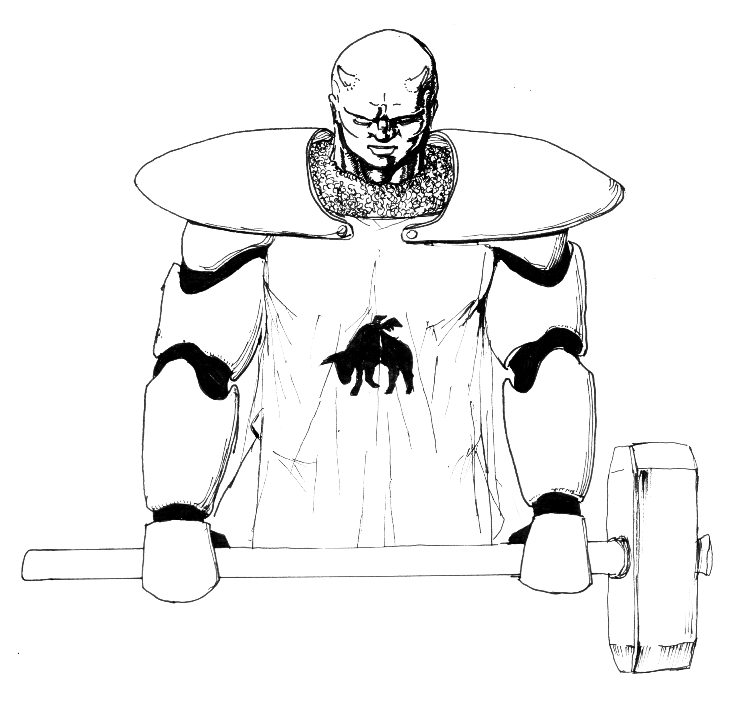
\includegraphics{baystbig.eps}
\end{center}
\end{figure*}

Bayst \`e capace di trasformarsi a piacimento in un enorme toro
bianco la cui cornata infligge 2d8 PV/PSC di danno. Come un toro, non
si cura degli ostacoli che si frappongono tra lui e la sua meta;
infatti la sua tattica prediletta di battaglia consiste nel caricare
gli avversari.

In forma umana combatte utilizzando un Martello da Guerra.
Allorch\'e viene privato di tale arma attacca con pugni e calci. Le
sue abilita di combattimento hanno un TOT pari all'AGI.

I Bayst possono attivare i poteri di: Eutanasia I, Filtro II, Infondi
Vita, Purificazione, Sfera di Immunit\`a, Trasferimento Vitale. 

\carmostro{13+1d10}{14+1d6}{20+1d10}{20+1d10}{20+1d10}{15+1d10}{12+1d10}{150}

\begin{parmostro}{Abilit\`a di Combattimento/TOT/Danno}
\item CAC/AGI/Danno normale
\item ABL/AGI/Danno normale
\end{parmostro}

\begin{parmostro}{Attacchi Particolari/TOT/Danno}
\item Corna/AGI/2d8
\end{parmostro}

\begin{parmostro}{Maestrie/TOT/BON}
\item Martello da Guerra/AGI
\end{parmostro}

\begin{parmostro}{Tecniche Speciali/TOT/BON}
\item Carica/1+BON AGI
\end{parmostro}

\begin{parmostro}{Difese}
\item  Armatura d'avorio (5 PP)
\end{parmostro}

\begin{parmostro}{Poteri Speciali}
\item Eutanasia I
\item Filtro II
\item Infondi Vita
\item Purificazione
\item Sfera di Immunit\`a
\item Trasferimento Vitale
\end{parmostro}

\begin{figure*}[t]
\begin{center}
{\it Johaim}\par\bigskip
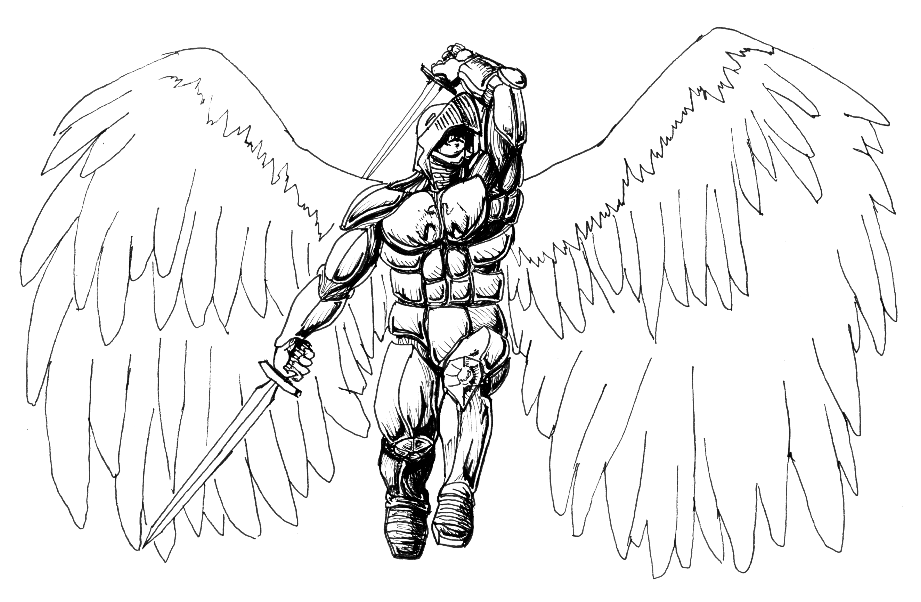
\includegraphics{johaim.eps}
\end{center}
\end{figure*}


\angelo{Johaim}{15}{Quarto Cielo}{Richiamabile}

Appare come un guerriero in armatura di bronzo con una protezione pari
a PP 8, con un elmo a forma di testa d'aquila che non toglie mai.

\`E provvisto di una coppia di ali d'argento che presentano margini
taglienti con le quali pu\`o attaccare ed infliggere 3d8 PV/PSC di
Danno.

Sulla sua armatura \`e raffigurata in bassorilievo un'aquila
d'argento.

Johaim pu\`o tramutarsi in un'aquila di bronzo il cui capo \`e
sormontato da una corona.

Nella forma umana impugna una spada in entrambe le mani. La sua
tattica preferita consiste nel librarsi in volo e attaccare da una
posizione sopraelevata. Le abilit\`a di combattimento hanno un TOT
pari alla sua AGI.

La voce risuona direttamente nella mente del suo interlocutore.

\`E in grado di attivare i poteri di: Eutanasia I, Evoca Angeli I,
Filtro II, Para Urti I, Resurrezione I, Riposo, Risveglio II, Sfera di
vita, Trasferimento Vitale

\carmostro{13+1d10}{14+1d6}{15+1d10}{20+1d10}{13+1d10}{14+1d8}{-}{180}

\begin{parmostro}{Abilit\`a di Combattimento/TOT/Danno}
\item CAC/AGI/Danno normale
\item ATL/AGI/Danno normale
\end{parmostro}

\begin{parmostro}{Attacchi Particolari/TOT/Danno}
\item Ali/AGI/3d8
\end{parmostro}

\begin{parmostro}{Maestrie/TOT/BON}
\item  Spada/AGI
\end{parmostro}

\begin{parmostro}{Tecniche di AM/TOT/BON}
\item Azioni multiple/20/+5
\end{parmostro}

\begin{parmostro}{Difese}
\item Armatura di bronzo (8 PP)
\end{parmostro}

\begin{parmostro}{Poteri speciali}
\item Eutanasia I
\item Evoca Angeli I
\item Filtro II
\item Para Urti I
\item Resurrezione I
\item Riposo
\item Risveglio II
\item Sfera di vita
\item Trasferimento Vitale
\end{parmostro}

\angelo{Custodi Maggiori}{19}{Quarto Cielo}{Richiamabili}

Hanno l'aspetto di uomini, elfi, gnomi, nani o qualsiasi altra razza,
circondati da una brillante luce azzurra che ne mette in risalto i
particolari somatici.  

Vestono le pi\`u svariate armature, dal cuoio
alle piastre e usano armi di qualunque tipo, di cui conoscono la
relativa Abilit\`a di Combattimento ad un TOT pari alla loro AGI.

Possono inoltre servirsi dei poteri di Cura III, DeviaColpo II,
Eutanasia I, Grandezza, Infondi Vita, Para Urti II, Resurrezione II,
Ricostruzione, Sfera di vita, Trasferimento Vitale. 

\carmostro{15+1d10}{14+1d8}{15+2d6}{20+1d10}{15+1d10}{14+1d8}{8+2d6}{225}

\begin{parmostro}{Abilit\`a di Combattimento/TOT/Danno}
\item CAC/AGI/Danno normale
\item ATL o ABL ecc./AGI/Danno normale
\end{parmostro}

\begin{parmostro}{Difese}
\item Armatura (1d8+2 PP)
\end{parmostro}

\begin{parmostro}{Poteri speciali}
\item Cura III
\item Devia Colpo II
\item Eutanasia I
\item Grandezza
\item Infondi Vita
\item Para Urti II
\item Resurrezione II
\item Ricostruzione
\item Sfera di vita
\item Trasferimento Vitale
\end{parmostro}

\angelo{Adonai}{20}{Terzo Cielo}{Richiamabile}

La sua forma \`e quella di un vecchio alto e robusto con i capelli e
la barba candidi e luminosi, che indossa un drappo bianco finemente
decorato. Sulla sua veste, \`e rappresentato un triangolo equilatero
con un occhio al centro.

L'unico punto vitale del suo corpo \`e il torace, che \`e protetto
dal triangolo (10 PP). La mutilazione di una qualunque altra parte del
suo corpo non ne determina la morte.

La sua voce \`e pari al rombo di un tuono; ci\`o implica la
realizzazione di un TR a difficolt\`a 25 per evitare di restare
storditi per il round in corso e quello successivo.

\pinup{adonai.eps}{Adonai}

Adonai combatte con CAC utilizzando in particolare Prese e Proiezioni
con un TOT pari alla sua AGI. La sua tattica preferita \`e quella di
bloccare l'avversario in un abbraccio e successivamente urlargli
contro.

\'E in grado di utilizzare i seguenti poteri: Cura III, Eutanasia II,
Guarigione III, Medicina, Para Urti II, Resurrezione II, Sfera di
Vita.

\carmostro{17+1d8}{16+1d8}{18+1d10}{20+1d10}{18+1d10}{17+1d8}{8+2d6}{240}

\begin{parmostro}{Abilit\`a di Combattimento/TOT/Danno}
\item CAC/AGI/Danno normale
\end{parmostro}

\begin{parmostro}{Attacchi Particolari/TOT/Danno}
\item Voce/TR a 25/Stordimento
\end{parmostro}

\begin{parmostro}{Specifiche di AM/TOT/BON}
\item Presa/AGI/BON Presa
\item  Proiezione/AGI/BON Proiezione
\end{parmostro}

\begin{parmostro}{Difese}
\item Triangolo (10 PP)
\end{parmostro}

\begin{parmostro}{Poteri Speciali}
\item Cura III
\item Eutanasia II
\item Guarigione III
\item Medicina
\item Para Urti II
\item Resurrezione II
\item Sfera di Vita
\end{parmostro}

\angelo{Uziel}{23}{Terzo Cielo}{Richiamabile} 

Ha l'aspetto di un giovane biondo e con i capelli lunghi, dai
lineamenti delicatissimi ed ambigui. Indossa un'armatura d'argento,
capace di proteggerlo con 10 PP, su cui \`e raffigurato un roveto
ardente.\`E dotato di due ali bianche simili a quelle delle colombe.

I suoi occhi brillano di una luce fiammeggiante, pertanto in chiunque
lo guardi in viso induce cecit\`a per 1d4+2 round se non si realizza
un TR a difficolt\`a 30, la voce ricorda un crepitare di fiamme.

Il suo elmo \`e dotato di una celata che abbassa alla bisogna.
Quando la celata \`e abbassata non \`e in grado di provocare la
cecit\`a. 

\`E fornito di un Arco Elfico e di un'Alabarda, che sa
usare alla perfezione. Solitamente si erge in volo ad una certa
distanza dall'avversario e inizia ad attaccare con l'arco. Se privato
delle armi, utilizza i calci. Utilizza l'alabarda anche per effettuare
una micidiale carica in picchiata. La carica ha bisogno di un round di
preparazione.

Le sue abilita di combattimento hanno un TOT pari all'AGI.

Pu\`o usare i poteri di: Devia Colpo II, Eutanasia II, Evoca Angeli I, Evoca
Angeli II, GuarigioneIII, Ibernazione, Incarnazione, Para Urti II, Raggio di
Luce, Resurrezione II. 

\carmostro{17+1d8}{16+1d8}{18+1d10}{20+1d10}{18+1d10}{17+1d8}{19+1d6}{260}

\begin{parmostro}{Abilit\`a di Combattimento/TOT/Danno}
\item CAC/AGI/Danno normale
\item ADT/AGI/Danno normale
\item AIA/AGI/Danno normale
\end{parmostro}

\begin{parmostro}{Attacchi Particolari/TOT/Danno}
\item Cecit\`a/TR a 30/Cecit\`a per 1d4
  round
\end{parmostro}

\begin{parmostro}{Maestrie/TOT/BON}
\item Alabarda/AGI 
\item Arco Elfico/AGI  
\end{parmostro}

\begin{parmostro}{Specifiche di AM/TOT/BON}
\item Calcio/AGI/BON Calcio
\end{parmostro}

\begin{parmostro}{Tecniche Speciali/TOT/BON}
\item Carica/AGI/BON Carica
\end{parmostro}

\begin{parmostro}{Difese}
\item Armatura d'argento (10 PP)
\end{parmostro}

\begin{parmostro}{Poteri speciali}
\item Devia Colpo II
\item Eutanasia II
\item Evoca Angeli I Evoca Angeli II
\item Guarigione III
\item Ibernazione
\item Incarnazione
\item Para Urti II
\item Raggio di Luce
\item Resurrezione II
\end{parmostro}

\angelo{Mikael}{$>$ 30}{Secondo Cielo}{Non Richiamabile}

Appare come un umano alto 2.5 metri, che indossa un'armatura dorata
su cui \`e incisa in bassorilievo una bilancia. Il suo volto pallido \`e
solcato da numerose rughe. 

I suoi occhi sono azzurri e i suoi lunghi capelli
neri sono mossi costantemente da una brezza leggera. \`E dotato di tre coppie
di ali. La sua voce \`e atona e il suo volto non tradisce alcun sentimento.

\angelo{Raphael}{$>$ 30}{Secondo Cielo}{Non Richiamabile} 

Appare come un giovane alto 2 metri e mezzo. I suoi capelli castani
sono lunghi e ricci e gli occhi sono verdi. Indossa, sopra ad una
veste rossa da pellegrino, un'armatura d'oro su cui \`e
raffigurato in bassorilievo un pesce. Impugna un lungo bastone.  Il
suo volto non mostra alcun sentimento. 

Possiede anch'egli tre coppie di ali.

\angelo{Gabriel}{$>$ 30}{Secondo Cielo}{Non Richiamabile} 

Appare come un uomo nel pieno della sua forma fisica, alto 2 metri e
mezzo. I suoi capelli biondi e lisci sono tagliati all'altezza della
nuca e i suoi occhi sono neri.

Indossa, sopra un'ampia tunica verde, un'armatura d'oro su cui
\`e cesellato un ramo d'ulivo. Impugna un grande scettro d'oro. Il
suo volto non mostra alcun sentimento. Possiede anch'egli tre coppie
di ali.

\angelo{Lucifer}{$>$ 30}{Primo Cielo}{Non Richiamabile}

\`E l'angelo che sta a capo della gerarchia. Alto un metro e 80,
appare dotato di tre volti ognuno mostrante un differente sentimento.

\`E dotato di quattro braccia e tre coppie di ali dorate. I suoi
capelli sono rossi, lunghi e ricci e gli occhi dorati. Indossa una
veste candida.

Di solito appare seduto su un trono, circondato da una moltitudine di
altri angeli. Rifulge di una luce talmente potente che lo si pu\`o
guardare soltanto per pochi secondi. 

Pu\`o assumere le sembianze di un qualunque essere vivente.

\subsection{Gli Incantesimi}
\label{incesistenza}
%----------------------------------------------------------------------------
\begin{spell}{Amputazione}{Esistenza}{Attacco}{Danno Mirato}
%----------------------------------------------------------------------------
\descrizione{Fa partire una lama luminosa che infligge 6d6 PV/PSC di danno mirato su un target a contatto col mago.}
%% DR DA DT DB MOD PM PF PE TL
\incvalori{28}{36}{5}{30}{1}{28}{9}{36}{4}
\parametro{Danno}{6}{d6}{30}
\parametro{Base TPC}{0}{}{0}
\fineparametri
\gittatanulla
\campo{1}{target}{2}
\duratanulla
\end{spell}
%----------------------------------------------------------------------------
\begin{spell}{Anestesia}{Esistenza}{Controllo}{Comando}
%----------------------------------------------------------------------------
\descrizione{Fa addormentare un target per 11 minuti se questo non realizza un TV a Diff. 15. Dopo la durata il target dorme per 2d6 ore se non viene svegliato.}
%% DR DA DT DB MOD PM PF PE TL
\incvalori{15}{29}{11}{15}{3}{15}{5}{29}{2}
\parametro{Difficolt\`a del TV}{15}{}{15}
\fineparametri
\gittatanulla
\campo{1}{target}{2}
\durata{11 min}{2}
\end{spell}
%----------------------------------------------------------------------------
\begin{spell}{Antidolore}{Esistenza}{Alterazione}{Variazione abilit\`a fisica}
%----------------------------------------------------------------------------
\descrizione{Conferisce al target un bonus di +10 all'abilit\`a Resistenza al Dolore per 3 minuti.}
%% DR DA DT DB MOD PM PF PE TL
\incvalori{16}{29}{18}{10}{1}{16}{5}{29}{2}
\parametro{Variazione abilit\`a}{10}{punti}{10}
\fineparametri
\gittatanulla
\campo{1}{target}{2}
\durata{3 min}{0}
\end{spell}
%----------------------------------------------------------------------------
\begin{spell}{Antishock}{Esistenza}{Controllo}{Variazione PSIche}
%----------------------------------------------------------------------------
\descrizione{Conferisce un bonus di +5 alla Psiche del target per 3 minuti. Il target si deve a trovare al massimo a 4 metri dal mago.}
%% DR DA DT DB MOD PM PF PE TL
\incvalori{4}{18}{10}{5}{3}{4}{1}{18}{1}
\parametro{Variazione caratteristica PSI}{5}{punti}{5}
\fineparametri
\gittata{4}{1}
\campo{1}{target}{2}
\durata{3 min}{0}
\end{spell}
%----------------------------------------------------------------------------
\begin{spell}{Asservimento Angeli I}{Esistenza}{Evocazione}{Controllo}
%----------------------------------------------------------------------------
\descrizione{Consente di controllare un Angelo della potenza massima di 12 per un periodo massimo di 3 minuti. Il mago pu\`o impartirgli ordini se vince un Confronto di TV con esso se \`e un essere errante, o con chi lo controlla, se \`e controllato da qualcuno.}
%% DR DA DT DB MOD PM PF PE TL
\incvalori{17}{29}{14}{12}{3}{17}{5}{29}{2}
\parametro{Potenza della creatura}{12}{}{12}
\fineparametri
\gittata{4}{1}
\campo{1}{target}{2}
\durata{3 min}{0}
\end{spell}
%----------------------------------------------------------------------------
\begin{spell}{Asservimento Angeli II}{Esistenza}{Evocazione}{Controllo}
%----------------------------------------------------------------------------
\descrizione{Consente di controllare un Angelo della potenza massima di 19 per un periodo di 3 minuti. Il mago pu\`o impartirgli ordini se vince un Confronto di TV con esso se \`e un essere errante, o con chi lo controlla se esso \`e gia controllato.}
%% DR DA DT DB MOD PM PF PE TL
\incvalori{24}{36}{14}{19}{3}{24}{8}{36}{4}
\parametro{Potenza della creatura}{19}{}{19}
\fineparametri
\gittata{4}{1}
\campo{1}{target}{2}
\durata{3 min}{0}
\end{spell}
%----------------------------------------------------------------------------
\begin{spell}{Asservimento Angeli III}{Esistenza}{Evocazione}{Controllo}
%----------------------------------------------------------------------------
\descrizione{Consente di controllare un Angelo della potenza massima di 23 per 3 minuti. Il mago pu\`o impartirgli ordini se vince un confronto di TV con esso se \`e un essere errante, o con chi lo domina se l'essere \`e gi\`a controllato.}
%% DR DA DT DB MOD PM PF PE TL
\incvalori{28}{40}{14}{23}{3}{28}{9}{40}{4}
\parametro{Potenza della creatura}{23}{}{23}
\fineparametri
\gittata{4}{1}
\campo{1}{target}{2}
\durata{3 min}{0}
\end{spell}
%----------------------------------------------------------------------------
\begin{spell}{Barella}{Esistenza}{Alterazione}{Spostamento sul piano}
%----------------------------------------------------------------------------
\descrizione{Fa apparire una barella che consente di trasportare un target posto a non pi\`u di 1 metro di distanza e pesante fino a 120 kg e con 100 kg di equipaggiamento alla velocit\`a di 10 km/h. L'incantesimo viene tenuto a concentrazione. Al venir meno della concentrazione l'effetto prosegue per 3 minuti.}
%% DR DA DT DB MOD PM PF PE TL
\incvalori{16}{29}{16}{6}{7}{16}{5}{29}{2}
\parametro{Massa vivente}{120}{kg}{4}
\parametro{Velocit\`a}{10}{km/h}{1}
\parametro{Massa non vivente}{100}{kg}{1}
\fineparametri
\gittata{1}{0}
\campo{1}{target}{2}
\durata{concentrazione+3 min}{5+0}
\end{spell}
%----------------------------------------------------------------------------
\begin{spell}{Bisturi}{Esistenza}{Alterazione}{Modifica Danni anatomia/armi}
%----------------------------------------------------------------------------
\descrizione{Allunga di 10 cm un'unghia del target, rendendola affilatissima e capace di infliggere 1d6 PV/PSC di danno. L'incantesimo perdura a concentrazione, pi\`u 3 minuti.}
%% DR DA DT DB MOD PM PF PE TL
\incvalori{19}{32}{20}{6}{6}{19}{6}{32}{3}
\parametro{Danno}{1}{d6}{5}
\parametro{Massa}{1}{kg}{1}
\fineparametri
\gittata{1}{0}
\campo{1}{m}{1}
\durata{concentrazione+3 min}{5+0}
\end{spell}
%----------------------------------------------------------------------------
\begin{spell}{Coraggio}{Esistenza}{Controllo}{Variazione VOLont\`a}
%----------------------------------------------------------------------------
\descrizione{Conferisce un bonus di +2 alla Volont\`a di un target posto a non pi\`u di un metro dal mago per la durata di tre minuti.}
%% DR DA DT DB MOD PM PF PE TL
\incvalori{19}{33}{19}{12}{2}{19}{6}{33}{3}
\parametro{Variazione caratteristica}{2}{punti}{12}
\fineparametri
\gittata{1}{0}
\campo{1}{target}{2}
\durata{3 min}{0}
\end{spell}
%----------------------------------------------------------------------------
\begin{spell}{Cura follia}{Esistenza}{Difesa}{Cura}
%----------------------------------------------------------------------------
\descrizione{Restituisce ad un target ad una distanza massima di 1 metro 1d6 di Psiche.}
%% DR DA DT DB MOD PM PF PE TL
\incvalori{5}{25}{21}{2}{2}{5}{1}{25}{1}
\parametro{Riparazione}{1}{d6}{2}
\fineparametri
\gittata{1}{0}
\campo{1}{target}{2}
\duratanulla
\end{spell}
%----------------------------------------------------------------------------
\begin{spell}{Cura I}{Esistenza}{Difesa}{Cura}
%----------------------------------------------------------------------------
\descrizione{Cura 1d6 PV/PSC di danno ad 1 target, purch\'e venga toccato dal mago. Delle ferite guarite non resta alcuna traccia.}
%% DR DA DT DB MOD PM PF PE TL
\incvalori{4}{24}{21}{2}{1}{4}{1}{24}{1}
\parametro{Riparazione}{1}{d6}{2}
\fineparametri
\gittatanulla
\campo{1}{target}{2}
\duratanulla
\end{spell}
%----------------------------------------------------------------------------
\begin{spell}{Cura II}{Esistenza}{Difesa}{Cura}
%----------------------------------------------------------------------------
\descrizione{Cura 3d6 PV/PSC di danno a tutti gli esseri che si trovano in un'area di 1 metro di raggio distante fino a 1 metro dall'usufruitore. Delle ferite guarite non resta alcuna traccia.}
%% DR DA DT DB MOD PM PF PE TL
\incvalori{8}{28}{21}{6}{1}{8}{2}{28}{1}
\parametro{Riparazione}{3}{d6}{6}
\fineparametri
\gittata{1}{0}
\campo{1}{m}{1}
\duratanulla
\end{spell}
%----------------------------------------------------------------------------
\begin{spell}{Cura III}{Esistenza}{Difesa}{Cura}
%----------------------------------------------------------------------------
\descrizione{Cura 7d6 PV/PSC di danno a tutti gli esseri che si trovano in un'area di 4 metro di raggio distante fino a 7 metri dall'usufruitore. Delle ferite guarite non resta alcuna traccia.}
%% DR DA DT DB MOD PM PF PE TL
\incvalori{19}{39}{21}{14}{4}{19}{6}{39}{3}
\parametro{Riparazione}{7}{d6}{14}
\fineparametri
\gittata{4}{1}
\campo{3}{m}{3}
\duratanulla
\end{spell}
%----------------------------------------------------------------------------
\begin{spell}{Devia Colpo I}{Esistenza}{Difesa}{Deviazione}
%----------------------------------------------------------------------------
\descrizione{Devia tutti gli attacchi diretti al target per 3 minuti, con Base TPD pari a 10.}
%% DR DA DT DB MOD PM PF PE TL
\incvalori{16}{36}{25}{10}{1}{16}{5}{36}{2}
\parametro{Base TPD}{10}{punti}{10}
\fineparametri
\gittatanulla
\campo{1}{target}{2}
\durata{3 min}{0}
\end{spell}
%----------------------------------------------------------------------------
\begin{spell}{Devia Colpo II}{Esistenza}{Difesa}{Deviazione}
%----------------------------------------------------------------------------
\descrizione{Devia tutti gli attacchi diretti al target per 3 minuti, con Base TPD pari a 20.}
%% DR DA DT DB MOD PM PF PE TL
\incvalori{26}{46}{25}{20}{1}{26}{8}{46}{4}
\parametro{Base TPD}{20}{punti}{20}
\fineparametri
\gittatanulla
\campo{1}{target}{2}
\durata{3 min}{0}
\end{spell}
%----------------------------------------------------------------------------
\begin{spell}{Erboristeria}{Esistenza}{Informazione}{Variazione abilit\`a mentale}
%----------------------------------------------------------------------------
\descrizione{Conferisce al target un bonus di +9 all'abilit\`a Conoscere Piante o +3 all'abilit\`a Alchimia, per 3 minuti.}
%% DR DA DT DB MOD PM PF PE TL
\incvalori{20}{28}{18}{9}{1}{20}{6}{28}{3}
\parametro{Variazione abilit\`a}{9}{punti}{9}
\fineparametri
\gittatanulla
\campo{1}{target}{2}
\durata{3 min}{0}
\end{spell}
%----------------------------------------------------------------------------
\begin{spell}{Eutanasia I}{Esistenza}{Attacco}{Morte}
%----------------------------------------------------------------------------
\descrizione{Offre il conforto della morte dolce ad un target. Se il target non vuole spegnersi dolcemente pu\`o vanificare l'effetto dell'incantesimo realizzando un TR a Diff. 10.}
%% DR DA DT DB MOD PM PF PE TL
\incvalori{21}{29}{18}{10}{1}{21}{7}{29}{3}
\parametro{Difficolt\`a del TR}{10}{}{10}
\fineparametri
\gittatanulla
\campo{1}{target}{2}
\duratanulla
\end{spell}
%----------------------------------------------------------------------------
\begin{spell}{Eutanasia II}{Esistenza}{Attacco}{Morte}
%----------------------------------------------------------------------------
\descrizione{Offre il conforto della morte dolce ad un target. Se il target non vuole spegnersi dolcemente pu\`o vanificare l'effetto dell'incantesimo realizzando un TR a Diff. 20.}
%% DR DA DT DB MOD PM PF PE TL
\incvalori{31}{39}{18}{20}{1}{31}{10}{39}{5}
\parametro{Difficolt\`a del TR}{20}{}{20}
\fineparametri
\gittatanulla
\campo{1}{target}{2}
\duratanulla
\end{spell}
%----------------------------------------------------------------------------
\begin{spell}{Evoca Angeli I}{Esistenza}{Evocazione}{Richiamo}
%----------------------------------------------------------------------------
\descrizione{Evoca un Caduto, un Rugiel o un Custode Minore per 3 minuti. Il mago pu\`o impartirgli ordini se vince un confronto di TV con esso.}
%% DR DA DT DB MOD PM PF PE TL
\incvalori{20}{32}{18}{12}{2}{20}{6}{32}{3}
\parametro{Potenza della creatura}{12}{}{12}
\fineparametri
\gittata{1}{0}
\campo{1}{target}{2}
\durata{3 min}{0}
\end{spell}
%----------------------------------------------------------------------------
\begin{spell}{Evoca Angeli II}{Esistenza}{Evocazione}{Richiamo}
%----------------------------------------------------------------------------
\descrizione{Evoca un Bayst, un Johaim o un Custode Maggiore (o Angeli di potenza inferiore) per 3 minuti. Il mago pu\`o impartirgli ordini se vince un confronto di TV con esso.}
%% DR DA DT DB MOD PM PF PE TL
\incvalori{27}{39}{18}{19}{2}{27}{9}{39}{4}
\parametro{Potenza della creatura}{19}{}{19}
\fineparametri
\gittata{1}{0}
\campo{1}{target}{2}
\durata{3 min}{0}
\end{spell}
%----------------------------------------------------------------------------
\begin{spell}{Evoca Angeli III}{Esistenza}{Evocazione}{Richiamo}
%----------------------------------------------------------------------------
\descrizione{Evoca un Uziel o un Adonai (o un Angelo di potenza inferiore) per 3 minuti. Il mago pu\`o impartirgli ordini se vince un confronto di TV con esso.}
%% DR DA DT DB MOD PM PF PE TL
\incvalori{31}{43}{18}{23}{2}{31}{10}{43}{5}
\parametro{Potenza della creatura}{23}{}{23}
\fineparametri
\gittata{1}{0}
\campo{1}{target}{2}
\durata{3 min}{0}
\end{spell}
%----------------------------------------------------------------------------
\begin{spell}{Filtro I}{Esistenza}{Difesa}{Scudo antidinamico}
%----------------------------------------------------------------------------
\descrizione{Crea un filtro di luce azzurra che rallenta tutti gli attacchi fisici o quelli magici di danno mirato diretti al target dividendone il danno per 2. L'incantesimo dura 3 minuti.}
%% DR DA DT DB MOD PM PF PE TL
\incvalori{12}{32}{21}{10}{1}{12}{4}{32}{2}
\parametro{Divisore}{2}{unit\`a}{10}
\fineparametri
\gittatanulla
\campo{1}{target}{2}
\durata{3 min}{0}
\end{spell}
%----------------------------------------------------------------------------
\begin{spell}{Filtro II}{Esistenza}{Difesa}{Scudo antidinamico}
%----------------------------------------------------------------------------
\descrizione{Crea un filtro di luce bianca che rallenta tutti gli attacchi fisici o quelli magici di danno mirato diretti al target dividendone il danno per 4. L'incantesimo dura 3 minuti.}
%% DR DA DT DB MOD PM PF PE TL
\incvalori{22}{42}{21}{20}{1}{22}{7}{42}{3}
\parametro{Divisore}{4}{unit\`a}{20}
\fineparametri
\gittatanulla
\campo{1}{target}{2}
\durata{3 min}{0}
\end{spell}
%----------------------------------------------------------------------------
\begin{spell}{Grandezza}{Esistenza}{Alterazione}{Variazione dimensioni}
%----------------------------------------------------------------------------
\descrizione{Dimezza o raddoppia le dimensioni di un target, posto a contatto col mago, pesante fino a 90 kg e che trasporti un equipaggiamento pesante fino a 100 kg. Il target pu\`o opporsi all'incantesimo realizzando un TR a Diff. 18. Dopo 3 minuti il target riprende le sue dimensioni normali.}
%% DR DA DT DB MOD PM PF PE TL
\incvalori{13}{26}{17}{8}{1}{13}{4}{26}{2}
\parametro{Massa vivente}{90}{kg}{3}
\parametro{Massa non vivente}{100}{kg}{1}
\parametro{Fattore dimensione}{2}{unit\`a}{4}
\fineparametri
\gittatanulla
\campo{1}{target}{2}
\durata{3 min}{0}
\end{spell}
%----------------------------------------------------------------------------
\begin{spell}{Guarigione I}{Esistenza}{Difesa}{Resurrezione}
%----------------------------------------------------------------------------
\descrizione{Guarisce in 1d6 giorni un target da una malattia mortale, se la somma del lancio di 5d6 supera il numero di PV originari del target (COSx3 + BON FOR escludendo le variazioni dovute a droghe, incantesimi, etc...) .}
%% DR DA DT DB MOD PM PF PE TL
\incvalori{9}{29}{21}{10}{-2}{9}{3}{29}{1}
\parametro{Riparazione}{5}{d6}{10}
\parametro{Tempo trascorso dalla morte}{0}{giorni}{0}
\fineparametri
\gittatanulla
\campo{1}{target}{2}
\durata{3 min}{0}
\azionetempo{1d6 giorni}{-3}
\end{spell}
%----------------------------------------------------------------------------
\begin{spell}{Guarigione II}{Esistenza}{Difesa}{Resurrezione}
%----------------------------------------------------------------------------
\descrizione{Guarisce in 1d6 giorni da una malattia mortale tutti gli esseri che si trovano in un'area di 3 metri di raggio con centro sul guaritore, se la somma del lancio di 10d6 supera il numero di PV originari dei target (COSx3 + BON FOR escludendo le variazioni dovute a droghe, incantesimi, etc...).}
%% DR DA DT DB MOD PM PF PE TL
\incvalori{20}{40}{21}{20}{-1}{20}{6}{40}{3}
\parametro{Riparazione}{10}{d6}{20}
\parametro{Tempo trascorso dalla morte}{0}{giorni}{0}
\fineparametri
\gittatanulla
\campo{3}{m}{3}
\duratanulla
\azionetempo{1d6 giorni}{-3}
\end{spell}
%----------------------------------------------------------------------------
\begin{spell}{Guarigione III}{Esistenza}{Difesa}{Resurrezione}
%----------------------------------------------------------------------------
\descrizione{Guarisce in 1d6 giorni da una malattia mortale tutti gli esseri che si trovano in un'area di 3 metri di raggio con centro sul guaritore, se la somma del lancio di 15d6 supera il numero di PV originari del target (COSx3 + BON FOR escludendo le variazioni dovute a droghe, incantesimi, etc...) .}
%% DR DA DT DB MOD PM PF PE TL
\incvalori{30}{50}{21}{30}{-1}{30}{10}{50}{5}
\parametro{Riparazione}{15}{d6}{30}
\parametro{Tempo trascorso dalla morte}{0}{giorni}{0}
\fineparametri
\gittatanulla
\campo{3}{m}{3}
\duratanulla
\azionetempo{1d6 giorni}{-3}
\end{spell}
%----------------------------------------------------------------------------
\begin{spell}{Ibernazione}{Esistenza}{Alterazione}{Variazione propriet\`a fisiche}
%----------------------------------------------------------------------------
\descrizione{Conserva permanentemente un corpo di massimo 120 kg di peso, abbassandone la temperatura interna. Pu\`o essere usato anche per conservare cadaveri o cibarie.}
%% DR DA DT DB MOD PM PF PE TL
\incvalori{34}{47}{15}{16}{16}{34}{11}{47}{5}
\parametro{Complessit\`a}{12}{}{12}
\parametro{Massa vivente}{120}{kg}{4}
\parametro{Massa non vivente}{0}{kg}{0}
\fineparametri
\gittatanulla
\campo{1}{target}{2}
\durata{permanente }{15}
\end{spell}
%----------------------------------------------------------------------------
\begin{spell}{Implanto}{Esistenza}{Alterazione}{Modifica Anatomia per nuove funzioni}
%----------------------------------------------------------------------------
\descrizione{Crea un secondo organo per coadiuvare le funzioni di un organo esistente, per 15 minuti.}
%% DR DA DT DB MOD PM PF PE TL
\incvalori{17}{30}{15}{11}{4}{17}{5}{30}{2}
\parametro{Complessit\`a}{10}{}{10}
\parametro{Massa vivente}{30}{kg}{1}
\parametro{Fattore dimensione}{0}{unit\`a}{0}
\fineparametri
\gittatanulla
\campo{1}{target}{2}
\durata{15 min}{3}
\end{spell}
%----------------------------------------------------------------------------
\begin{spell}{Incarnazione}{Esistenza}{Controllo}{Possessione}
%----------------------------------------------------------------------------
\descrizione{Come Trasferimento Vitale, ma l'usufruitore si incarna definitivamente nel corpo del target, fino allo scioglimento dell'incantesimo. Alla morte del corpo originario del mago, l'incantesimo non potr\`a pi\`u essere sciolto.}
%% DR DA DT DB MOD PM PF PE TL
\incvalori{33}{47}{11}{20}{16}{33}{11}{47}{5}
\parametro{Difficolt\`a del TV}{20}{}{20}
\fineparametri
\gittatanulla
\campo{1}{target}{2}
\durata{permanente }{15}
\end{spell}
%----------------------------------------------------------------------------
\begin{spell}{Infondi vita}{Esistenza}{Alterazione}{Creazione Esseri Viventi}
%----------------------------------------------------------------------------
\descrizione{Dona la vita a tutti gli oggetti inanimati inclusi in un'area di 1 metro di raggio, di piccole dimensioni, fino a 30 kg di massa totale (sassi, tavolini, suppellettili) conferendo loro un numero massimo di PCAT di 40. L'incantesimo infonde la vita in 1d6 giorni.}
%% DR DA DT DB MOD PM PF PE TL
\incvalori{24}{37}{29}{11}{-3}{24}{8}{37}{4}
\parametro{Massa vivente}{30}{kg}{1}
\parametro{punti CAraTteristica}{40}{punti}{10}
\fineparametri
\gittatanulla
\campo{1}{m}{1}
\duratanulla
\azionetempo{1d6 giorni}{-3}
\end{spell}
%----------------------------------------------------------------------------
\begin{spell}{Medicina}{Esistenza}{Informazione}{Variazione abilit\`a mentale}
%----------------------------------------------------------------------------
\descrizione{Attribuisce al target un bonus di +5 all'abilit\`a Medicina per 15 minuti.}
%% DR DA DT DB MOD PM PF PE TL
\incvalori{29}{37}{18}{15}{4}{29}{9}{37}{4}
\parametro{Variazione abilit\`a}{15}{punti}{15}
\fineparametri
\gittatanulla
\campo{1}{target}{2}
\durata{15 min}{3}
\end{spell}
%----------------------------------------------------------------------------
\begin{spell}{Para Urti I}{Esistenza}{Difesa}{Parata}
%----------------------------------------------------------------------------
\descrizione{Crea due sfere luminose orbitanti attorno al target aventi lo scopo di parare ciascuna un attacco diretto ad esso, con Base TPD pari a 20. Ognuna delle sfere scompare dopo aver parato un attacco. Le sfere scompaiono comunque dopo 3 minuti.}
%% DR DA DT DB MOD PM PF PE TL
\incvalori{20}{40}{15}{24}{1}{20}{6}{40}{3}
\parametro{Base TPD}{20}{punti}{20}
\parametro{Parate}{2}{}{4}
\fineparametri
\gittatanulla
\campo{1}{target}{2}
\durata{3 min}{0}
\end{spell}
%----------------------------------------------------------------------------
\begin{spell}{Para Urti II}{Esistenza}{Difesa}{Parata}
%----------------------------------------------------------------------------
\descrizione{Crea 5 sfere luminose orbitanti attorno al target aventi lo scopo di parare ciascuna un attacco diretto ad esso, con Base TPD pari a 20. Ognuna delle sfere scompare dopo aver parato un attacco. Le sfere scompaiono comunque dopo 3 minuti.}
%% DR DA DT DB MOD PM PF PE TL
\incvalori{26}{46}{15}{30}{1}{26}{8}{46}{4}
\parametro{Base TPD}{20}{punti}{20}
\parametro{Parate}{5}{}{10}
\fineparametri
\gittatanulla
\campo{1}{target}{2}
\durata{3 min}{0}
\end{spell}
%----------------------------------------------------------------------------
\begin{spell}{Protezione Angeli I}{Esistenza}{Evocazione}{Protezione}
%----------------------------------------------------------------------------
\descrizione{Viene creata attorno al mago un'area di 3 metri di raggio all'interno della quale gli angeli di potenza inferiore o uguale a 12 non possono entrare se non realizzando un TV a Diff. 22. Realizzando un TV le creature potranno avanzare di 1 metro, subendo 1d6 PV di danno netto per ogni metro all'interno dell'area, L'incantesimo scompare se un essere all'interno dell'area protetta attacca le creature dalle quali si sta proteggendo. Per ogni metro all'interno dell'area il TV delle creature \`e penalizzato di -1. L'incantesimo perdura per 3 minuti.}
%% DR DA DT DB MOD PM PF PE TL
\incvalori{12}{24}{10}{12}{2}{12}{4}{24}{2}
\parametro{Potenza della creatura}{12}{}{12}
\fineparametri
\gittatanulla
\campo{3}{m}{3}
\durata{3 min}{0}
\end{spell}
%----------------------------------------------------------------------------
\begin{spell}{Protezione Angeli II}{Esistenza}{Evocazione}{Protezione}
%----------------------------------------------------------------------------
\descrizione{Viene creata attorno al mago un'area di 3 metri di raggio all'interno della quale gli angeli di potenza inferiore o uguale a 19 non possono entrare se non realizzando un TV a Diff. 29 Realizzando un TV le creature potranno avanzare di 1 metro, subendo 1d6 PV di danno netto per ogni metro all'interno dell'area, L'incantesimo scompare se un essere all'interno dell'area protetta attacca le creature dalle quali si sta proteggendo. Per ogni metro all'interno dell'area il TV delle creature \`e penalizzato di -1. L'incantesimo perdura per 3 minuti.}
%% DR DA DT DB MOD PM PF PE TL
\incvalori{19}{31}{10}{19}{2}{19}{6}{31}{3}
\parametro{Potenza della creatura}{19}{}{19}
\fineparametri
\gittatanulla
\campo{3}{m}{3}
\durata{3 min}{0}
\end{spell}
%----------------------------------------------------------------------------
\begin{spell}{Protezione Angeli III}{Esistenza}{Evocazione}{Protezione}
%----------------------------------------------------------------------------
\descrizione{Viene creata attorno al mago un'area di 3 metri di raggio all'interno della quale gli angeli di potenza inferiore o uguale a 23 non possono entrare se non realizzando un TV a Diff. 33. Realizzando un TV le creature potranno avanzare di 1 metro, subendo 1d6 PV di danno netto per ogni metro all'interno dell'area, L'incantesimo scompare se un essere all'interno dell'area protetta attacca le creature dalle quali si sta proteggendo. Per ogni metro all'interno dell'area il TV delle creature \`e penalizzato di -1. L'incantesimo perdura per 3 minuti.}
%% DR DA DT DB MOD PM PF PE TL
\incvalori{23}{35}{10}{23}{2}{23}{7}{35}{3}
\parametro{Potenza della creatura}{23}{}{23}
\fineparametri
\gittatanulla
\campo{3}{m}{3}
\durata{3 min}{0}
\end{spell}
%----------------------------------------------------------------------------
\begin{spell}{Purificazione}{Esistenza}{Alterazione}{Variazione propriet\`a fisiche}
%----------------------------------------------------------------------------
\descrizione{Sterilizza cibo e acqua fino ad una massa totale di 100 kg. Se il cibo purificato non viene conservato in maniera idonea entro 3 minuti, potr\`a nuovamente andare a male.}
%% DR DA DT DB MOD PM PF PE TL
\incvalori{9}{22}{15}{7}{0}{9}{3}{22}{1}
\parametro{Complessit\`a}{6}{}{6}
\parametro{Massa vivente}{0}{kg}{0}
\parametro{Massa non vivente}{100}{kg}{1}
\fineparametri
\gittatanulla
\campo{1}{m}{1}
\durata{3 min}{0}
\end{spell}
%----------------------------------------------------------------------------
\begin{spell}{Raggio di luce}{Esistenza}{Attacco}{Danno Netto}
%----------------------------------------------------------------------------
\descrizione{Investe un target di un lampo luminoso di energia che gli infligge 10d6 PV (Pi\`u eventuali Danni Addizionali da ustione) di danno netto dimezzabile con un TR a Diff. 30. L'incantesimo deve essere effettuato a contatto.}
%% DR DA DT DB MOD PM PF PE TL
\incvalori{34}{42}{21}{20}{1}{34}{11}{42}{5}
\parametro{Danno}{10}{d6}{20}
\fineparametri
\gittatanulla
\campo{1}{target}{2}
\duratanulla
\end{spell}
%----------------------------------------------------------------------------
\begin{spell}{Restauro}{Esistenza}{Difesa}{Riparazione danni}
%----------------------------------------------------------------------------
\descrizione{Ripara danni a tutti gli oggetti posti all'interno di un'area di 3 metri di raggio, per un totale di 5d6 Punti Struttura per ogni oggetto. Il centro dell'area di 3 metri pu\`o distare fino ad 1 metro dal mago.}
%% DR DA DT DB MOD PM PF PE TL
\incvalori{8}{28}{15}{10}{3}{8}{2}{28}{1}
\parametro{Riparazione}{5}{d6}{10}
\fineparametri
\gittata{1}{0}
\campo{3}{m}{3}
\duratanulla
\end{spell}
%----------------------------------------------------------------------------
\begin{spell}{Resurrezione I}{Esistenza}{Difesa}{Resurrezione}
%----------------------------------------------------------------------------
\descrizione{Resuscita un target se il risultato del lancio di 7d6 supera o eguaglia il numero totale dei PV originari del target (COSx3 + BON FOR escludendo gli effetti di droghe, incantesimi, etc...), purch\'e non sia trascorso pi\`u di 1 giorno dal decesso.}
%% DR DA DT DB MOD PM PF PE TL
\incvalori{17}{37}{21}{15}{1}{17}{5}{37}{2}
\parametro{Riparazione}{7}{d6}{14}
\parametro{Tempo trascorso dalla morte}{1}{giorno}{1}
\fineparametri
\gittatanulla
\campo{1}{target}{2}
\durata{3 min}{0}
\end{spell}
%----------------------------------------------------------------------------
\begin{spell}{Resurrezione II}{Esistenza}{Difesa}{Resurrezione}
%----------------------------------------------------------------------------
\descrizione{Resuscita un target se il risultato del lancio di 10d6 supera o eguaglia il numero totale dei PV originari del target (COSx3 + BON FOR escludendo gli effetti di droghe, incantesimi, etc...), purch\'e non siano trascorsi pi\`u di 5 giorni dal decesso.}
%% DR DA DT DB MOD PM PF PE TL
\incvalori{27}{47}{21}{25}{1}{27}{9}{47}{4}
\parametro{Riparazione}{10}{d6}{20}
\parametro{Tempo trascorso dalla morte}{5}{giorni}{5}
\fineparametri
\gittatanulla
\campo{1}{target}{2}
\durata{3 min}{0}
\end{spell}
%----------------------------------------------------------------------------
\begin{spell}{Ricostruzione}{Esistenza}{Difesa}{Riparazione danni}
%----------------------------------------------------------------------------
\descrizione{Ripara danni a tutti gli oggetti posti all'interno di un'area di 10 metri di raggio, per un totale di 10d6 Punti Struttura per ogni oggetto. Il centro dell'area di 10 metri pu\`o distare fino a 4 metri dal mago. I danni verranno riparati gradualmente in 1d6 giorni.}
%% DR DA DT DB MOD PM PF PE TL
\incvalori{23}{43}{15}{20}{8}{23}{7}{43}{3}
\parametro{Riparazione}{10}{d6}{20}
\fineparametri
\gittata{4}{1}
\campo{10}{m}{10}
\durata{3 min}{0}
\azionetempo{1d6 giorni}{-3}
\end{spell}
%----------------------------------------------------------------------------
\begin{spell}{Riposo}{Esistenza}{Difesa}{Cura}
%----------------------------------------------------------------------------
\descrizione{Restituisce al target 4d6 PF o 4d6 PM.}
%% DR DA DT DB MOD PM PF PE TL
\incvalori{10}{30}{21}{8}{1}{10}{3}{30}{1}
\parametro{Riparazione}{4}{d6}{8}
\fineparametri
\gittatanulla
\campo{1}{target}{2}
\duratanulla
\end{spell}
%----------------------------------------------------------------------------
\begin{spell}{Risveglio I}{Esistenza}{Difesa}{Rianimazione}
%----------------------------------------------------------------------------
\descrizione{Rianima dal coma un target se il risultato del lancio di 5d6 eguaglia o supera il numero totale dei PV originari del target (COSx3 + BON FOR escludendo gli effetti di droghe, incantesimi, etc...).}
%% DR DA DT DB MOD PM PF PE TL
\incvalori{6}{26}{15}{10}{1}{6}{2}{26}{1}
\parametro{Riparazione}{5}{d6}{10}
\fineparametri
\gittatanulla
\campo{1}{target}{2}
\duratanulla
\end{spell}
%----------------------------------------------------------------------------
\begin{spell}{Risveglio II}{Esistenza}{Difesa}{Rianimazione}
%----------------------------------------------------------------------------
\descrizione{Rianima dal coma un target se il risultato del lancio di 10d6 eguaglia o supera il numero totale dei PV originari del target (COSx3 + BON FOR escludendo gli effetti di droghe, incantesimi, etc...).}
%% DR DA DT DB MOD PM PF PE TL
\incvalori{16}{36}{15}{20}{1}{16}{5}{36}{2}
\parametro{Riparazione}{10}{d6}{20}
\fineparametri
\gittatanulla
\campo{1}{target}{2}
\duratanulla
\end{spell}
%----------------------------------------------------------------------------
\begin{spell}{Sfera di immunit\`a}{Esistenza}{Difesa}{Protezione Magica}
%----------------------------------------------------------------------------
\descrizione{Protegge tutti i target che stanno all'interno di un'area di 1 metro di raggio, distante fino a 1 metro dall'usufruitore, da ogni incantesimo di Attacco/Danno netto, assorbendo 7d6 di danno, nel corso di 3 minuti.}
%% DR DA DT DB MOD PM PF PE TL
\incvalori{15}{35}{20}{14}{1}{15}{5}{35}{2}
\parametro{Protezione}{7}{d6}{14}
\fineparametri
\gittata{1}{0}
\campo{1}{m}{1}
\durata{3 min}{0}
\end{spell}
%----------------------------------------------------------------------------
\begin{spell}{Sfera di vita}{Esistenza}{Difesa}{Armatura}
%----------------------------------------------------------------------------
\descrizione{Crea una sfera di 1 metro di raggio che garantisce una protezione pari a 10 PP a tutti coloro che stanno al suo interno. La protezione dura 3 minuti.}
%% DR DA DT DB MOD PM PF PE TL
\incvalori{20}{40}{19}{20}{1}{20}{6}{40}{3}
\parametro{Protezione}{10}{PP}{20}
\fineparametri
\gittata{1}{0}
\campo{1}{m}{1}
\durata{3 min}{0}
\end{spell}
%----------------------------------------------------------------------------
\begin{spell}{Trasferimento vitale}{Esistenza}{Controllo}{Possessione}
%----------------------------------------------------------------------------
\descrizione{L'usufruitore trasferisce la sua essenza vitale all'interno di un ospite per 15 minuti. Durante questo tempo il corpo dell'usufruitore rester\`a in catalessi. Il target potr\`a sottrarsi all'incantesimo realizzando un TV a Diff. 20.}
%% DR DA DT DB MOD PM PF PE TL
\incvalori{21}{35}{11}{20}{4}{21}{7}{35}{3}
\parametro{Difficolt\`a del TV}{20}{}{20}
\fineparametri
\gittatanulla
\campo{1}{target}{2}
\durata{15 min}{3}
\end{spell}



%%---------------------------------------------------------------------------
\vfill\section{Illusionismo}
%%---------------------------------------------------------------------------

\Simbolo{simb_ill.eps}

L'altra parte del regno Memath,  l'Illusionismo, o Magia dell'Illusione
in Novese o Via del Pensiero in Elfico, presiede i poteri della mente e
dell'inconscio.

Simbolo degli illusionisti sono tre cerchi concentrici con un occhio
aperto stilizzato nel centro.

\subsection{Dominio}

Tutti gli incantesimi degli illusionisti sono legati
ai poteri della mente, e hanno a che fare con i pensieri e i sogni
delle creature. La scuola dell'Illusionismo \`e in contatto magico
con la Dimora Onirica, sede degli Incubi e dei Sogni dei viventi. Le
creature oniriche possono essere richiamate nel mondo reale solo dagli
illusionisti. 

L'esistenza della Dimora Onirica \`e determinata dai
sogni dei vivi. Gli oggetti che vi si trovano non sono permanenti, per
la maggior parte appaiono e scompaiono spesso repentinamente,
cos\`{\i} come i pensieri e i sogni degli uomini. 

Nella Dimora Onirica
qualsiasi oggetto pu\`o essere creato semplicemente desiderandolo e
quasi tutti gli oggetti possono essere distrutti o modificati nello
stesso modo. Esattamente quello che avviene nei sogni. 

Nell'Onirica le creature sono riunite in cinque Dimore in ordine di
potere. Ogni dimora \`e alimentata dagli incubi e dai sogni
dell'et\`a relativa. 

\begin{description} 
\item{\bf La Quinta Dimora} ospita gli incubi e i sogni degli esseri
  pensanti \textbf{adulti} e maturi. Per evocare un essere di V dimora
  \`e necessario che ci sia un dormiente di quell'et\`a a meno di
  1000 metri da chi tenta il richiamo.
  
\item{\bf La Quarta Dimora} ospita gli incubi e i sogni degli esseri
  pensanti che hanno da poco\textbf{ oltrepassato la maturit\`a.}
  Per evocare un essere di IV dimora \`e necessario che ci sia un
  dormiente di quell'et\`a a meno di 1000 metri da chi tenta il
  richiamo.
  
\item{\bf La Terza Dimora} ospita gli incubi e i sogni degli esseri
  pensanti che hanno superato l'infanzia ma non sono ancora giunti
  alla soglia dell'et\`a adulta. Per evocare un essere di III dimora \`e
  necessario che ci sia un dormiente di quell'et\`a a meno di 1000
  metri da chi tenta il richiamo.
  
\item{\bf La Seconda Dimora} ospita gli incubi e i sogni degli esseri
  pensanti dell'et\`a senile. Gli esseri onirici di seconda dimora
  non si possono richiamare, ma talvolta autonomamente oltrepassano il
  confine della dimora onirica per introdursi nel mondo reale.
  
\item{\bf La Prima Dimora} ospita gli incubi e i sogni degli esseri
  pensanti che attraversano l'infanzia. Essa \`e permeata
  dall'essenza del Babau.
\end{description}

\subsection{Limiti e peculiarit\`a}

Solo gli illusionisti possono evocare e controllare le creature
dell'incubo e del sogno. Per evocare un essere onirico della 3$^a${
  d}imora bisogna che, nel raggio di 1 km, un ``adolescente'', di
qualsiasi specie animale, stia sognando. Per evocare un essere onirico
della 4$^a${ d}imora bisogna che, nel raggio di 1 km, un ``anziano''
di qualsiasi specie animale stia sognando. Per evocare un essere
onirico della 5$^a${ d}imora bisogna che, nel raggio di 1 km, un
``adulto'' di qualsiasi specie animale stia sognando.

Solo gli illusionisti sono in grado di proiettare la loro coscienza
all'interno della dimora onirica, e cos\`{\i} influenzare i sogni dei
dormienti. Per fare ci\`o devono effettuare la seguente
``cerimonia'':
\begin{itemize}
\item Realizzare un TCONC a 25
\item Realizzare un tiro sulla scuola di magia Illusionismo a
  difficolt\`a 20
\item Addormentarsi per almeno 30 minuti
\item Realizzare un Confronto di TV con un dormiente, scelto come
  ``porta di accesso'' alla dimora onirica, che si deve trovare a meno
  di 10 metri da loro.
\end{itemize}

Se la ``porta'' si sveglia il contatto consapevole con la dimora
onirica si scioglie. Il mago si pu\`o svegliare a sua volta
realizzando un TCONC a 20. In caso di fallimento del TCONC il mago
continuer\`a a dormire.

In caso di
riuscita il mago potr\`a decidere se svegliarsi o continuare a
dormire. 

Se anche uno solo dei 4 ``passi'' della cerimonia non va a
buon fine, essa non riesce. Il mago potr\`a addormentarsi e
continuare a dormire senza poter influenzare i sogni altrui. Il mago
consumer\`a 1 PE per ogni TV tentato nella Dimora Onirica. Gli
adepti dell'illusionismo infliggono il danno magicamente, mediante
``danni illusori'', ``convincendo'' le vittime degli incantesimi di
aver subito danni. Il danno illusorio toglie PV e PSC esattamente come
il danno reale. 

I Danni Illusori si infliggono come qualsiasi
incantesimo di Attacco.

\subsection{Potenzialit\`a} 
\begin{tabular}{lc}
Evocazione& 14\\
Alterazione& 9 \\
Controllo& 20 \\
Informazione& 16\\
Difesa& 11 \\
Attacco& 5\\
\end{tabular}

\subsection{Leggi dell'uso}
\begin{enumerate}\itemsep -6pt
\item Non lasciare liberi gli esseri onirici
\item Non annullare la volont\`a di un Arcimago 
\end{enumerate}


\subsection{Gli Esseri Onirici}

Gli Esseri Onirici, detti anche Creature Oniriche, si dividono in due
grandi categorie: Incubi e Sogni. 

Gli incubi e i sogni hanno vita e volont\`a proprie e risiedono
perennemente nella dimora onirica, di cui fanno parte e a cui sono
rigidamente legati.

Il loro comportamento \`e illogico e caotico.  Se due creature
oniriche si incontrano, generalmente intraprendono un cruento
combattimento all'ultimo sangue, indipendentemente dalla differenza di
forza tra i due, ma a volte capita che si ignorino o (pi\`u
raramente) che si alleino per uno scopo comune.

In ogni caso per ogni creatura onirica distrutta se ne
rigenera dopo un certo tempo una simile, in modo tale che il numero delle creature
oniriche sia sempre strettamente legato al numero di viventi. 

Tutte queste creature possono assumere nella Dimora Onirica la forma e
l'aspetto che desiderano, comprese le forme geometriche o di oggetti
invisibili, bench\'e ogni specie ne abbia una preferita.

In genere gli incubi sono molto brutti, schifosi o raccapriccianti,
mentre i sogni sono solitamente belli e gradevoli agli occhi dei
sognatori.  I sogni e gli incubi non sentono dolore e sono immuni alle
malattie.

Per sconfiggerli \`e necessario inabilitarli, portare a 0 i loro PV,
distruggere totalmente il corpo o distruggere il punto vitale tipico
della specie. 

Se parti dei loro corpi vengon danneggiate o distrutte durante i
combattimenti, essi perdono i PV e i PSC ed eventualmente le
funzionalit\`a della parte amputata.

\es{Un incubo che ha gli occhi sulla testa viene decapitato. La testa
  non \`e il punto vitale tipico della sua specie, quindi continua
  tranquillamente a muoversi e a combattere (con i malus per la
  perdita dei PV), ma perde la capacit\`a di vedere}

Se vengono ``divisi'' in pi\`u parti, solo una di esse sopravvive.

Una volta ridotti a 0 i loro PV, anche se il loro corpo non \`e
stato totalmente disintegrato, essi scompaiono.

Una volta evocati, gli incubi e i sogni perdono il potere di creare
oggetti, e assumono la forma tipica della loro razza, conservando
per\`o la capacit\`a di alterare gli stati d'animo e l'indole
originaria: gli incubi sono generalmente crudeli, i sogni sono di
indole buona, bench\'e entrambe le classi siano assolutamente
caotiche e imprevedibili. 

I sogni e gli incubi (sia nella loro forma nativa che in quella
concreta che assumono in seguito all'evocazione) hanno sommariamente
poteri dello stesso livello e sono in grado incutere nel sognatore una
sensazione tipica della razza a cui appartengono.

Generalmente gli incubi (da qui il loro nome) tendono a incutere
dolore, paura, terrore o ansia, mentre i sogni si orientano verso una
semplice indifferenza o verso allegria, benessere o piacere.

Sia i sogni che gli incubi sono suddivisi in cinque Dimore, di potenza
crescente dalla quinta alla prima.  

Per evocare una creatura onirica, deve esserci almeno un sognatore
adatto (per et\`a o indole) nel raggio di 1000 metri. La creatura
evocata scompare se tutti i sognatori in tale raggio si svegliano.

Mentre la Diff. di Conoscere un incubo \`e generalmente pari alla sua
Potenza $+10$, la difficolt\`a di conoscere un sogno \`e pari alla sua
Potenza $+15$.

\subsubsection{Le raffigurazioni} 

Le raffigurazioni sono gli esseri od oggetti sognati dai vivi. Possono
essere modificate o distrutte con la volont\`a (in tal caso
scompaiono dal sogno) e create con la stessa.  In entrambi i casi
occorre effettuare un Confronto di TV tra il costruttore e il
distruttore.

Le raffigurazioni possono essere concretizzate. In tal caso vengono
``spostate'' dal sogno al piano materiale e spariscono definitivamente
dal sogno (il sognatore pu\`o comunque ricrearle al sogno
successivo, dopo essersi svegliato). Una raffigurazione \`e solo la
rappresentazione di un oggetto o di una persona, ed \`e pertanto
priva di quasi tutte le funzionalit\`a tipiche.

Una spada concretizzata quindi pu\`o non tagliare (ma pu\`o essere
sempre usata allo scopo di percuotere).  Un uomo (o un essere vivente)
concretizzato pu\`o non pensare o agire per conto proprio, ma
si comporta come un automa, eseguendo gesti stereotipati o
pronunciando frasi ovvie o senza senso.

Una raffigurazione concretizzata non pu\`o avere caratteristiche
superiori a quelle dell'oggetto che rappresenta e pu\`o essere solo
leggermente differente per struttura, dimensioni e proporzioni;
inoltre non pu\`o avere poteri magici di alcun tipo. 

In termini di gioco l'incantesimo di concretizzazione di una
raffigurazione si deve classificare nel tipo ``Alterazione/ Creazione
Oggetti'' o ``Alterazione/ Creazione Esseri Viventi''.

Una raffigurazione, comunque, non pu\`o superare il punteggio di 5
nel TOT per nessuna abilit\`a. 

Un particolare tipo di raffigurazione \`e l'\textbf{alter ego}, ossia
l'idea che un sognatore ha di se stesso nel sogno. Tale raffigurazione
non pu\`o essere evocata n\`e fatta scomparire con un TV e ha
caratteristiche pari a quelle del sognatore, meno 10 (la bellezza non
subisce il malus).

L'alter ego si comporta in un sogno pi\`u o meno come farebbe il
sognatore stesso, bench\'e le azioni compiute siano per lo pi\`u
illogiche e confuse. 

Uccidendo un alter ego il sognatore si sveglia.

Le informazioni raccolte dall'alter ego vengono acquisite dal
sognatore al risveglio se questo realizza un TCONC a 20, in caso
contrario il sognatore dimentica il sogno. 

\incubo{Braak}{5}{Quinta Dimora}{Richiamabile}

Assumono la forma di un grosso sacco azzurro a chiazze gialle,
carnoso, con la parte inferiore coperta di peli bianchi, e la parte
superiore setolosa. Hanno una grande bocca irregolare irta di denti
triangolari affilati e un numero di occhi variabile tra uno e cinque,
tutti disposti in fila orizzontale al di sopra della bocca.

Possiedono due, quattro, cinque o sette braccia (se le braccia sono in
numero dispari, una di esse si incastra sulla sommit\`a della
``testa'') lunghe e sottili, con mani e dita lunghissime, appuntite e
affusolate.

\pinup{braak.eps}{Braak}

Si muovono volando non troppo rapidamente a pochi centimetri da terra
(ma possono raggiungere una quota anche elevata) e raggiungono le
dimensioni di un uomo alto e robusto.  Combattono a mani nude
sfruttando le loro armi naturali: il grosso pugno che pu\`o
infliggere 2d6 PV/PSC di danno; la stretta delle lunghe dita, che
infligge 1d8 PV/PSC di danno, e il morso, che infligge 1d6 PV/PSC di
danno. La superficie del loro corpo \`e coriacea e li protegge per
un valore di 1 PP. Il loro punto vitale \`e il grosso torace.

\carmostro{6+1d6}{4+2d8}{10+2d6}{10+1d6}{10+2d6}{4+3d6}
{3-1d6}{45}

\begin{parmostro}{Abilit\`a di Combattimento/TOT/Danno}
\item CAC/AGI-3/Danno Normale
\end{parmostro}

\begin{parmostro}{Attacchi Particolari/TOT/Danno}
\item Pugno/AGI/2d6
\item Presa/AGI/1d8
\item Morso/AGI-4/1d6
\end{parmostro}

\begin{parmostro}{Difese}
\item Pelle coriacea (PP 1)
\end{parmostro}

\begin{parmostro}{Poteri speciali}
\item Paralisi I
\item Sonno I
\end{parmostro}

\incubo{Greyant}{6}{Quinta  Dimora}{Richiamabile}

Se evocati appaiono come delle formiche grigie lunghe dai due ai
quattro metri.

Hanno due occhi composti di colore arancione debolmente luminosi, che
conferiscono loro un'aspetto spettrale. Il corpo \`e
completamente ricoperto di peli grigi che puzzano di muffa. 

Sulla testa hanno due coppie di mandibole che usano per torturare e
stritolare e sono muniti di otto zampe. Una volta individuato un
bersaglio, lo catturano e non lo abbandonano fino alla sua morte, se
non per una fuga strategica. 

Il loro morso infligge 2d8 PV/PSC di danno. 

Il loro guscio esterno funziona come una armatura, proteggendoli per 5
PP. Se si esclude un fischio raccapricciante, sono completamente muti.
Il loro punto vitale \`e la testa.

\carmostro{4+1d6}{4+2d8}{15+1d10}{4+1d6}{15+1d10}{4+1d6} {-}{60}

\begin{parmostro}{Abilit\`a di combattimento/TOT/Danno}
\item CAC/AGI/Danno Normale
\end{parmostro}

\begin{parmostro}{Attacchi Particolari/TOT/Danno}
\item Morso/AGI-1/2d8 
\end{parmostro}

\begin{parmostro}{Difese}
\item Corazza (PP 5)
\end{parmostro}

\begin{parmostro}{Poteri Speciali}
\item Buio
\item Fetore
\item Paralisi I
\item Paura I
\end{parmostro}

\sogno{Blink}{6}{Quinta Dimora}{Richiamabile}

Si presenta come una lucina puntiforme e multicolore in continuo
movimento.  Si sposta fluttuando lentamente fino a 4 m da terra (o
dall'acqua), \`e capace di effettuare scatti velocissimi fino ad 1
metro (1 scatto per round al massimo) ed \`e in grado di introdursi
in qualunque apertura, compresi gli orifizi corporei. 

La sua forza si manifesta sotto forma di un'onda di pressione sferica
con centro nella lucina e raggio 50 cm, che funziona come una
Proiezione che infligge 2d6 PV/PSC di danno.

Se colpito la sua luce si affievolisce, fino a
spegnersi del tutto alla sua morte. I suoi colpi permessi di CAC sono
limitati a Schivare, Divincolarsi, Caduta. Non ha punti vitali, ma non
\`e molto resistente ai colpi. 

\`E in grado di comunicare esclusivamente con la telepatia ed ha una
tendenza particolare agli scherzi. Suscita divertimento.

\carmostro{10+1d6}{4+2d8}{6+1d6}{10+1d10}{6+1d10}{4+2d8} {-}{75}

\begin{parmostro}{Abilit\`a di Combattimento/TOT/Danno}
\item CAC/AGI/1d4
\end{parmostro}

\begin{parmostro}{Specifiche di AM/TOT/BON}
\item Schivare/20/+5
\end{parmostro}

\begin{parmostro}{Attacchi Particolari/TOT/Danno}
\item Onda di pressione/AGI/2d6
\end{parmostro}

\begin{parmostro}{Poteri speciali}
\item Ilarit\`a 
\item Paralisi I
\item Sonno I
\end{parmostro}



\incubo{Bleargh}{9}{Quarta Dimora}{Richiamabile}

Se evocati appaiono come un ammasso pi\`u o meno informe di tessuti
organici umidicci e puzzolenti, da cui si dipartono diverse appendici
con funzioni differenti: quelle oculari (bulbi oculari peduncolati),
quelle uncinate (ganci ossei, capaci di infliggere 2d6 PV/PSC di
danno) e quelle a ventosa attraverso le quali possono risucchiare la
``forza'' (assorbendo 2d4+1 PF) dei loro avversari.

Le Ventose vengono usate per effettuare Prese. I Bleargh non brandiscono
armi. Si muovono molto rapidamente strisciando o ondeggiando su
pseudopodi o tentacoli. Sono comunque molto sensibili ai colpi e non
hanno una grande forza. Un solo punto del loro corpo a scelta del
Master \`e da considerare ``punto vitale''.

\carmostro{10+1d6}{8+2d6}{6+1d6}{15+1d10}{6+1d6}{10+1d20}
{-1d6}{85} 

\begin{parmostro}{Abilit\`a di combattimento/TOT/Danno}
\item CAC/AGI/Danno Normale
\end{parmostro}

\begin{parmostro}{Attacchi Particolari/TOT/Danno}
\item Uncini/AGI/2d6 
\item Ventosa/AGI-2/2d4+1 PF
\end{parmostro}

\pinup{bleargh.eps}{Bleargh}

\begin{parmostro}{Poteri speciali}
\item Buio
\item Evoca Essere Onirico I
\item Invisibilit\`a
\item Ipnosi I
\item Paralisi I
\item Sonno II
\end{parmostro}

\sogno{Succubi}{9}{Quarta Dimora}{Richiamabile}

Si presentano come esseri bellissimi, nudi, della stessa razza ed
etnia dell'illusionista che li evoca, il quale \`e in grado di
stabilire il loro sesso (eventuale) solo se riesce vincere il
confronto di TV. 

Scopo della loro esistenza \`e quello di causare il piacere sensuale
dei viventi.

Sono molto astuti, agili e veloci nei movimenti ma non sono dotati di
una grande forza. Compensano la loro debolezza con sensi molto
sviluppati e una notevole capacit\`a di seduzione, che costituisce la
loro peculiarit\`a.

Possono risucchiare la forza (assorbendo 2d6 PF) della loro
``vittima'' attraverso il caratteristico bacio.

Hanno l'abilit\`a Sedurre ad un TOT pari alla BEL; per difendersi
tentano sempre di sedurre l'attaccante con ogni mezzo. 

Il loro punto vitale \`e l'addome.

\carmostro{10+1d6}{8+2d6}{6+1d6}{15+1d10}{6+1d6}{10+1d20}{16+1d6}{85}

\begin{parmostro}{Abilit\`a di combattimento/TOT/Danno}
\item CAC/AGI/Danno Normale
\end{parmostro}

\begin{parmostro}{Specifiche di AM/TOT/BON}
\item Presa/10/+3
\end{parmostro}

\begin{parmostro}{Attacchi Particolari/TPC/DANNO}
\item Bacio/AGI-2/2d6 PF
\end{parmostro}

\begin{parmostro}{Poteri speciali}
\item Buio
\item Invisibilit\`a
\item Ipnosi I
\item Lussuria
\item Paralisi I
\item Sonno II
\end{parmostro}


\incubo{Tolden}{12}{Quarta Dimora}{Richiamabile}

\begin{figure*}[bt]
{\centering\it Tolden\par
\includegraphics{tolden.eps}}
\end{figure*}

Ha l'aspetto di un gigantesco roditore, lungo fino a 3 metri, glabro
con la grossa testa incredibilmente sproporzionata rispetto al corpo.
Si sposta lentamente su 4 minuscole zampe ed \`e dotato di vibrisse
lunghe fino a 4 metri con le quali pu\`o infliggere danni da
elettricit\`a pari a 1d8 PV/PSC di danno o respingere attacchi da
arma da tiro, come la Tecnica Speciale Parare Frecce.

\`E quasi completamente cieco ma individua le sue prede con olfatto,
udito e ``sesto senso'' particolarmente sviluppati. \`E in grado di
scavare molto rapidamente e di spostarsi sottoterra alla velocit\`a
di 4 metri/sec se si trova su terreni non rocciosi (es. argilla,
fango, sabbia). Il suo morso \`e un'arma temibile in grado di
3d6+2 PV/PSC di danno. La sua pelle \`e dura e gli conferisce una
protezione di 4 PP. Il suo punto vitale \`e l'addome.

\carmostro{1d6}{8+2d6}{15+1d10}{10+1d10}{15+1d10} {2d4}{-1d6}{120}

\begin{parmostro}{Abilit\`a di combattimento/TOT/Danno}
\item CAC/AGI/Danno Normale
\end{parmostro}

\begin{parmostro}{Specifiche di AM/TOT/BON}
\item Parare/1+BON AGI
\end{parmostro}

\begin{parmostro}{Tecniche Speciali/TOT}
\item Parare frecce/AGI
\end{parmostro}

\begin{parmostro}{Attacchi Particolari/TOT/Danno}
\item Vibrissa/OSS+5/1d8
\item Morso/AGI/3d6+2
\end{parmostro}

\begin{parmostro}{Difese}
\item Pelle coriacea (PP 4)
\end{parmostro}

\begin{parmostro}{Poteri Speciali}
\item Barriera Psichica II
\item Cecit\`a
\item Dolore
\item Paralisi II
\item Sonno II
\item Stordimento
\end{parmostro}

\sogno{Moae}{12}{Quarta Dimora}{Richiamabile}

Ha l'aspetto di un enorme Uccello del Paradiso, con la coda
lunghissima e la livrea colorata e sgargiante. Si muove volando e
detesta stare con i viventi, tanto che difficilmente viene evocato. \`E
in grado di intonare splendide melodie con il suo dolce e acuto canto
capace di stordire i suoi avversari. \`E in grado di sollevare e
trasportare due o tre persone sul suo dorso.

La sua arma \`e costituita da un lampo luminoso che emette dalla
coda, funzionante come una Sfera Sonica. Per allontanarsi \`e capace
di rendersi invisibile ed ha una grande abilit\`a nello schivare gli
attacchi. Solitamente non parla, ma \`e in grado di farlo. Per
comunicare preferisce usare il suo canto o la telepatia. Combatte se
costretto attaccando con le zampe e il becco che infliggono 1d4 PV/PSC
di danno. Il suo punto vitale \`e la testa.

\carmostro{10+1d10}{8+2d6}{10+2d6}{10+2d6}{15+1d10}{
4+2d8}{-}{105} 

\begin{parmostro}{Abilit\`a di combattimento/TOT/Danno}
\item CAC/AGI/1d4
\end{parmostro}

\begin{parmostro}{Specifiche di AM/TOT}
\item  Schivare/AGI+15
\end{parmostro}

\begin{parmostro}{Poteri speciali}
\item Invisibilit\`a
\item Sdoppiamento
\item Sfera sonica
\item Stordimento
\end{parmostro}

\incubo{Kartenius}{15}{Quarta Dimora}{Richiamabile}

Appare come un'ombra nera corporea, con una sagoma umanoide magra,
curva ed incappucciata. Probabilmente \`e l'``Uomo Nero'' delle
storielle che si raccontano ai bambini. Il suo ``terreno'' di
movimento \`e il buio, o in sua assenza, le ombre. Non pu\`o
essere evocato se nella zona dell'evocatore non c'\`e una superficie
in ombra o al buio di dimensioni pari a quelle dell'Illusionista.  Se
viene illuminato violentemente fugge nella dimora onirica. \`E in grado
di nascondersi e spostarsi nelle ombre, se contigue, e nel buio
confondendosi con loro, per attaccare di sorpresa, e perci\`o viene
spesso evocato per utilizzarlo come assassino.

Kartenius si diverte a bloccare le sue vittime, a terrorizzarle e
infine ad ucciderle con le sue lunghissime unghie dopo averle
seviziate. Altre volte, dopo aver immobilizzato le sue vittime,
conduce con s\`e le loro menti nella dimora onirica, dove pu\`o
utilizzare meglio i suoi malefici poteri per renderle pazze,
riportandole nel Piano Materiale dopo aver svolto il suoi macabro
compito.

Non pu\`o essere colpito (ma non pu\`o neanche colpire) mentre
assume la forma dell'ombra. Il suo punto vitale \`e il torace.

\carmostro{10+2d6}{8+2d6}{8+1d6}{15+1d10}{8+1d6}{4+2d8}{-}{165}

\begin{parmostro}{Abilit\`a di combattimento/TOT/Danno}
\item CAC/AGI/Danno Normale
\end{parmostro}

\begin{parmostro}{Specifiche di AM/TOT/BON}
\item PREsa/10/+3
\end{parmostro}

\begin{parmostro}{Attacchi particolari/TOT/Danno}
\item Unghiata/AGI/1d6+3
\end{parmostro}

\begin{parmostro}{Altre Abilit\`a/TOT}
\item Nascondersi nell'ombra/AGI+5
\end{parmostro}

\begin{parmostro}{Poteri Speciali}
\item Barriera Psichica II
\item Buio
\item Dolore
\item Lettura del Pensiero
\item Pazzia
\item Sonno II
\item Velo d'ombra
\end{parmostro}


\incubo{Krull}{21}{Terza Dimora}{Richiamabile}

Appaiono come esseri composti da parti diverse di animali (ad esempio,
corpo umano con testa di falco, chele di granchio e coda di
coccodrillo oppure, ad esempio, corpo di insetto con occhi di lumaca e
bocca di tigre). Sono intelligenti e molto cattivi. Se non
controllati si accaniscono immediatamente contro l'evocatore, tentando
di controllarlo o bloccarlo prima di ucciderlo per avere il gusto di
torturarlo.

\pinup{krull.eps}{Krull}

Sono molto forti, attaccano come gli animali da cui sono composti,
(es. morso di serpente, zampata di tigre, codata di coccodrillo,
calcio di zebra) e si muovono rapidamente.  Sono molto abili nel
difendersi dagli attacchi. Possono avere parti del corpo ricoperte da
difese fisiche (schiena di granchio, chele di aragosta, ecc.).



\carmostro{7+3d6}{12+1d8}{19+1d6}{12+1d10}{15+2d10}{
10+2d10}{4-1d10}{300} 

\begin{parmostro}{Abilit\`a di combattimento/TOT/Danno}
\item CAC/AGI/Danno Normale
\end{parmostro}

\begin{parmostro}{Specifiche di AM/TOT/BON}
\item  Schivare/AGI Parare/AGI
\item Divincolarsi/AGI
\end{parmostro}


\begin{parmostro}{Difese}
\item Armature composite (PP variabili)
\end{parmostro}

\begin{parmostro}{Poteri Speciali}
\item Ipnosi III
\item Istigazione al Suicidio
\item Lettura del Pensiero
\item Panico
\item Quadruplicazione
\item Sonno Profondo
\item Telecinesi
\end{parmostro}

\sogno{Hukei}{21}{Terza Dimora}{Richiamabile}

Evocati diventano esseri mutaforma capaci di assumere a piacimento
l'aspetto di una pantera, un'aquila o un delfino. In tutte e tre le
forme sono completamente di color argento e hanno dimensioni circa
doppie rispetto all'animale rappresentato. 

Sotto forma di pantera si possono spostare a grande velocit\`a sulla
terra, in forma d'aquila si muovono volando e in forma di delfino
possono compiere spostamenti nell'acqua, sia in superficie che in
profondit\`a. 

Combattono utilizzando le armi naturali degli animali che
rappresentano.  Normalmente non attaccano e non usano i poteri se non
per difendersi.  In forma di pantera sono in grado di parlare, e in
tutte e tre le forme sono in grado di stabilire, con un essere
pensante che dista da loro meno di 50 metri, un collegamento
telepatico che rimane attivo anche se l'essere si allontana fino a 1
km di distanza.

La loro superficie simile al metallo costituisce un'ottima difesa (PP
8). 

Il loro punto vitale \`e la testa.

\carmostro{7+3d6}{12+1d8}{19+1d6}{12+1d10}{15+2d10}{
  10+2d10}{19+1d6}{300}

\begin{parmostro}{Abilit\`a di combattimento/TOT/Danno}
\item CAC/AGI/Danno Normale
\end{parmostro}

\begin{parmostro}{Attacchi Particolari/TOT/Danno}
\item  Pantera: Artiglio o Morso/AGI/3d6
\item Aquila: Becco/AGI/1d10+2
\item  Delfino: Testata/AGI/2d10
\end{parmostro}

\begin{parmostro}{Specifiche di AM/TOT/BON}
\item Schivata/AGI/BON Schivata
\item  Parata/AGI/BON Parata
\item  Divincolarsi/AGI/BON Divincolarsi
\end{parmostro}

\begin{parmostro}{Tecniche Speciali/TOT}
\item Carica/AGI
\end{parmostro}

\begin{parmostro}{Difese}
\item  Rivestimento metallico (PP 8)
\end{parmostro}

\begin{parmostro}{Poteri Speciali}
\item Ipnosi III
\item Istigazione al Suicidio
\item Lettura del Pensiero
\item Panico
\item Quadruplicazione
\item Sonno Profondo
\item Telecinesi
\end{parmostro}


\begin{figure*}[bth]
\begin{center}
{\it Benair}\par\bigskip
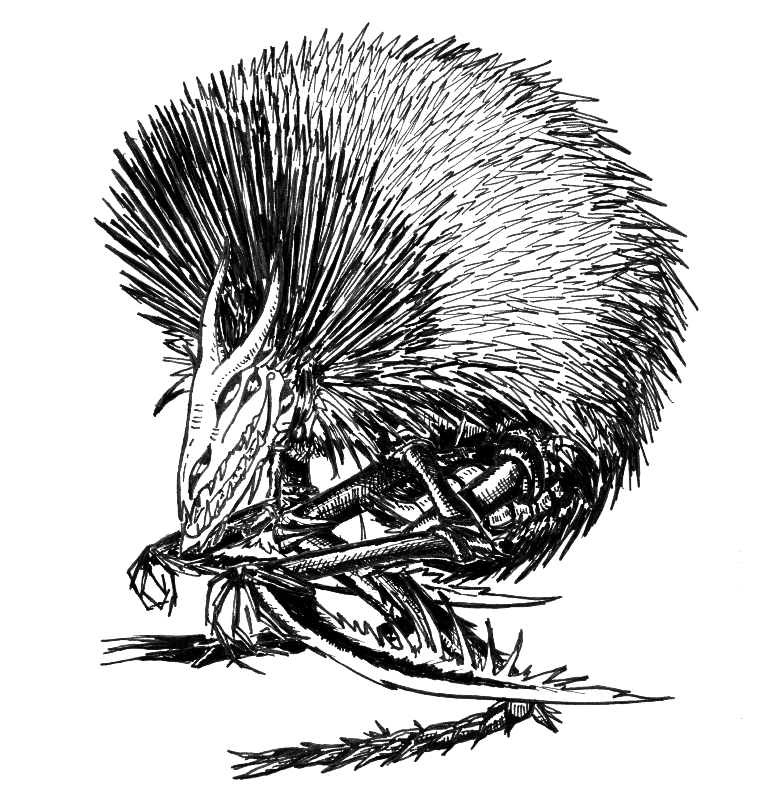
\includegraphics{benahir.eps}
\end{center}
\end{figure*}

\incubo{Benair}{23}{Terza Dimora}{Richiamabile}

Sono i pi\`u potenti tra gli incubi evocabili. Alti fino a 4 metri,
sono tozzi, scuri, curvi, hanno la schiena irta di aculei fitti,
lunghi e spessi, che possono lanciare a volont\`a. Gli arti
inferiori sono simili alle zampe di una mosca e l'addome \`e simile
a quello di un ragno. Gli arti superiori sono lunghi e
all'estremit\`a, oltre ad avere una sottilissima mano, in
corrispondenza dei polsi sono armati di affilatissime e lunghe lame
ossee, molto mobili e articolabili, con le quali possono colpire uno o
pi\`u bersagli fino a 5 m di distanza, come fossero dei lunghi
spadoni, infliggendo loro 3d8 PV/PSC di danno. La testa, allungata,
\`e provvista di bocca, in grado di mordere infliggendo 2d8 PV/PSC
di danno, e cheliceri, con un numero variabile di occhi rossi (6 o 8
sono comuni).  

Possono, a discrezione, parlare o comunicare per via
telepatica.

Sono in grado di avvolgersi a palla e di proiettarsi sui bersagli che
si trovano davanti a loro, su una linea retta, devastandoli con una
carica che infligge 5d6 PV/PSC di danno + FOR. Hanno bisogno per\`o
di 1 round per appallottolarsi.  Il loro unico punto vitale \`e
l'addome, che pu\`o essere colpito solo dal basso.

\carmostro{15+1d10}{12+1d8}{14+2d8}{14+2d8}{20+1d10}{15+1d10}{-1d10}{260}

\begin{parmostro}{Abilit\`a di Combattimento/TOT/Danno}
\item ATL/AGI/3d8
\item CAC/AGI/2d8
\item ADT/OSS+7/2d6
\end{parmostro}

\begin{parmostro}{Attacchi Particolari/TOT/Danno}
\item  Attacco a Palla/AGI/5d6
\end{parmostro}

\begin{parmostro}{Specifiche di AM/TOT}
\item Parata/AGI
\item Schivata/AGI
\end{parmostro}

\begin{parmostro}{Tecniche Speciali di AM/TOT}
\item Carica/AGI
\end{parmostro}

\begin{parmostro}{Difese}
\item Corazza di Spine (PP 10)
\end{parmostro}

\begin{parmostro}{Poteri Speciali}
\item Dolore
\item Evoca Essere Onirico II
\item Ipnosi III
\item Quadruplicazione
\item Realt\`a Virtuale
\item Scomparsa Totale
\item Scudo Psichico II
\item Sdoppiamento
\item Telecinesi
\item Tempesta di frecce
\item Viaggio Onirico
\end{parmostro}

\incubo{Morte}{$>$ 30}{Seconda Dimora}{Non Richiamabile}

L'unico essere onirico di seconda dimora di cui si abbia conoscenza
\`e l'incubo denominato Morte.

Non si conosce granch\'e di questa essenza; si sa soltanto che appare ai
vegliardi come un essere umanoide alto due metri e mezzo, vestito con
un saio scuro. Il suo viso \`e nascosto da un cappuccio dal quale si
intravedono gli occhi rossi. Regge in mano una grande falce. Non si
conoscono con esattezza i suoi poteri.


\incubo{Babau}{$>$ 30}{Prima Dimora}{Non Richiamabile}

Il Babau si manifesta raramente. \`E una creatura misteriosa, caotica,
potentissima; pu\`o apparire sotto qualsiasi aspetto e bench\'e sia
classificato come incubo non \`e ben chiaro se lo sia effettivamente
o sia un sogno.  Non esistono descrizioni pi\`u accurate.

Si sa per certo che esiste una sola entit\`a chiamata Babau, e si
suppone che questa sia la creatura pi\`u potente che abita la dimora
onirica.

\subsection{Gli Incantesimi}
\label{incillusionismo}
%----------------------------------------------------------------------------
\begin{spell}{Barriera psichica I}{Illusionismo}{Difesa}{Antimagia}
%----------------------------------------------------------------------------
\descrizione{Difende il target da tutti gli incantesimi a lui diretti nel tempo di 3 minuti, con una Base Antimagia di 10.}
%% DR DA DT DB MOD PM PF PE TL
\incvalori{15}{26}{15}{10}{1}{15}{5}{26}{2}
\parametro{Base antimagia}{10}{punti}{10}
\fineparametri
\gittatanulla
\campo{1}{target}{2}
\durata{3 min}{0}
\end{spell}
%----------------------------------------------------------------------------
\begin{spell}{Barriera psichica II}{Illusionismo}{Difesa}{Antimagia}
%----------------------------------------------------------------------------
\descrizione{Difende il target da tutti gli incantesimi nel tempo di 3 minuti, con una Base Antimagia di 20.}
%% DR DA DT DB MOD PM PF PE TL
\incvalori{25}{36}{15}{20}{1}{25}{8}{36}{4}
\parametro{Base antimagia}{20}{punti}{20}
\fineparametri
\gittatanulla
\campo{1}{target}{2}
\durata{3 min}{0}
\end{spell}
%----------------------------------------------------------------------------
\begin{spell}{Buio}{Illusionismo}{Controllo}{Illusione visiva}
%----------------------------------------------------------------------------
\descrizione{Illude i target che si trovano in un'area di 4 metri di raggio sita fino a 4 metri dal mago che la luce sia scomparsa. I target che realizzeranno un TOSS a Diff. 20 si renderanno conto che il buio \`e un'illusione e potranno rivedere la luce realizzando un TV a Diff. 20. Il buio dura 3 minuti.}
%% DR DA DT DB MOD PM PF PE TL
\incvalori{7}{27}{2}{20}{5}{7}{2}{27}{1}
\parametro{Difficolt\`a del TV e del TOSS}{20}{}{20}
\fineparametri
\gittata{4}{1}
\campo{4}{m}{4}
\durata{3 min}{0}
\end{spell}
%----------------------------------------------------------------------------
\begin{spell}{Cecit\`a}{Illusionismo}{Controllo}{Illusione visiva}
%----------------------------------------------------------------------------
\descrizione{Provoca la cecit\`a in 1 target posto ad una distanza massima di 4 metri illudendolo di essere perennemente al buio. Se il target realizza un TOSS a Diff. 25 si accorger\`a che la cecit\`a \`e un'illusione e potr\`a riprendere la vista realizzando un TV a Diff. 25.}
%% DR DA DT DB MOD PM PF PE TL
\incvalori{25}{45}{2}{25}{18}{25}{8}{45}{4}
\parametro{Difficolt\`a del TV e del TOSS}{25}{}{25}
\fineparametri
\gittata{4}{1}
\campo{1}{target}{2}
\durata{permanente }{15}
\end{spell}
%----------------------------------------------------------------------------
\begin{spell}{Concretizzazione}{Illusionismo}{Alterazione}{Creazione Esseri Viventi}
%----------------------------------------------------------------------------
\descrizione{Crea un essere vivente con massimo 30 Punti CAT richiamando dalla dimora onirica una raffigurazione di un essere vivente.}
%% DR DA DT DB MOD PM PF PE TL
\incvalori{33}{42}{29}{11}{2}{33}{11}{42}{5}
\parametro{Massa vivente}{90}{kg}{3}
\parametro{punti CAraTteristica}{30}{punti}{8}
\fineparametri
\gittata{1}{0}
\campo{1}{target}{2}
\durata{3 min}{0}
\end{spell}
%----------------------------------------------------------------------------
\begin{spell}{Concretizzazione oggetti}{Illusionismo}{Alterazione}{Creazione Oggetti}
%----------------------------------------------------------------------------
\descrizione{Crea un oggetto richiamando dalla dimora onirica una raffigurazione non vivente di un oggetto di massimo 30 kg di peso, di complessit\`a massima 8. L'oggetto sparisce dopo 3 minuti.}
%% DR DA DT DB MOD PM PF PE TL
\incvalori{21}{30}{19}{9}{2}{21}{7}{30}{3}
\parametro{Complessit\`a}{8}{}{8}
\parametro{Massa non vivente}{30}{kg}{1}
\fineparametri
\gittata{1}{0}
\campo{1}{target}{2}
\durata{3 min}{0}
\end{spell}
%----------------------------------------------------------------------------
\begin{spell}{Controllo Creatura Onirica I}{Illusionismo}{Evocazione}{Controllo}
%----------------------------------------------------------------------------
\descrizione{Consente di controllare il comportamento di una creatura onirica di potenza massima 6, situata a massimo 4 metri di distanza dal mago, per 3 minuti. Perch\'e il controllo abbia luogo, il mago deve vincere un Confronto di TV con la creatura se questa \`e una creatura errante, o realizzare un TV maggiore del TV effettuato da colui che ne ha il controllo.}
%% DR DA DT DB MOD PM PF PE TL
\incvalori{9}{23}{14}{6}{3}{9}{3}{23}{1}
\parametro{Potenza della creatura}{6}{}{6}
\fineparametri
\gittata{4}{1}
\campo{1}{target}{2}
\durata{3 min}{0}
\end{spell}
%----------------------------------------------------------------------------
\begin{spell}{Controllo Creatura Onirica II}{Illusionismo}{Evocazione}{Controllo}
%----------------------------------------------------------------------------
\descrizione{Consente di controllare il comportamento di una creatura onirica di potenza massima 15, situata a massimo 4 metri di distanza dal mago, per 3 minuti. Perch\'e il controllo abbia luogo, il mago deve vincere un Confronto di TV con la creatura se questa \`e una creatura errante o realizzare un TV maggiore del TV effettuato da colui che ne ha gi\`a il controllo.}
%% DR DA DT DB MOD PM PF PE TL
\incvalori{18}{32}{14}{15}{3}{18}{6}{32}{3}
\parametro{Potenza della creatura}{15}{}{15}
\fineparametri
\gittata{4}{1}
\campo{1}{target}{2}
\durata{3 min}{0}
\end{spell}
%----------------------------------------------------------------------------
\begin{spell}{Controllo Creatura Onirica III}{Illusionismo}{Evocazione}{Controllo}
%----------------------------------------------------------------------------
\descrizione{Consente di controllare il comportamento di una creatura onirica di potenza massima 23, situata a massimo 4 metri di distanza dal mago, per 3 minuti. Perch\'e il controllo abbia luogo, il mago deve vincere un Confronto di TV con la creatura se questa \`e una creatura errante o realizzare un TV maggiore del TV effettuato da colui che ha il controllo della creatura stessa.}
%% DR DA DT DB MOD PM PF PE TL
\incvalori{26}{40}{14}{23}{3}{26}{8}{40}{4}
\parametro{Potenza della creatura}{23}{}{23}
\fineparametri
\gittata{4}{1}
\campo{1}{target}{2}
\durata{3 min}{0}
\end{spell}
%----------------------------------------------------------------------------
\begin{spell}{Dolore}{Illusionismo}{Attacco}{Danno Netto}
%----------------------------------------------------------------------------
\descrizione{Provoca una brusca contrazione involontaria della muscolatura del target causando una dolorosa fitta che provoca 3d6 PV di danno. Il danno pu\`o essere dimezzato realizzando un TR a Diff. 16.}
%% DR DA DT DB MOD PM PF PE TL
\incvalori{25}{30}{21}{6}{3}{25}{8}{30}{4}
\parametro{Danno}{3}{d6}{6}
\fineparametri
\gittata{4}{1}
\campo{1}{target}{2}
\duratanulla
\end{spell}
%----------------------------------------------------------------------------
\begin{spell}{Evoca Essere Onirico I}{Illusionismo}{Evocazione}{Richiamo}
%----------------------------------------------------------------------------
\descrizione{Il mago richiama dalla dimora onirica un Braak, un Blink o un Greyant e gli impartisce comandi, che la creatura onirica esegue al meglio delle sue possibilit\`a, a patto che il mago vinca un confronto di TV con l'essere evocato. Perch\'e il richiamo riesca ci deve essere un adulto che dorme nel raggio di 1000 metri.}
%% DR DA DT DB MOD PM PF PE TL
\incvalori{12}{26}{18}{6}{2}{12}{4}{26}{2}
\parametro{Potenza della creatura}{6}{}{6}
\fineparametri
\gittata{1}{0}
\campo{1}{target}{2}
\durata{3 min}{0}
\end{spell}
%----------------------------------------------------------------------------
\begin{spell}{Evoca Essere Onirico II}{Illusionismo}{Evocazione}{Richiamo}
%----------------------------------------------------------------------------
\descrizione{Il mago richiama dalla dimora onirica un Bleargh, un Succube, un Tolden, un Moae o un Kartenius (o una creatura onirica di potenza inferiore) e gli impartisce comandi, che la creatura esegue al meglio delle sue possibilit\`a, a patto che il mago vinca un confronto di TV con l'essere evocato. Perch\'e il richiamo riesca ci deve essere un anziano che dorme nel raggio di 1000 metri.}
%% DR DA DT DB MOD PM PF PE TL
\incvalori{21}{35}{18}{15}{2}{21}{7}{35}{3}
\parametro{Potenza della creatura}{15}{}{15}
\fineparametri
\gittata{1}{0}
\campo{1}{target}{2}
\durata{3 min}{0}
\end{spell}
%----------------------------------------------------------------------------
\begin{spell}{Evoca Essere Onirico III}{Illusionismo}{Evocazione}{Richiamo}
%----------------------------------------------------------------------------
\descrizione{Il mago richiama dalla dimora onirica un Krull o un Benair (o una creatura onirica di potenza inferiore) e gli impartisce comandi, che la creatura esegue al meglio delle sue possibilit\`a, a patto che il mago vinca un confronto di TV con l'essere evocato. Perch\'e il richiamo riesca ci deve essere un adolescente che dorme nel raggio di 1000 metri.}
%% DR DA DT DB MOD PM PF PE TL
\incvalori{29}{43}{18}{23}{2}{29}{9}{43}{4}
\parametro{Potenza della creatura}{23}{}{23}
\fineparametri
\gittata{1}{0}
\campo{1}{target}{2}
\durata{3 min}{0}
\end{spell}
%----------------------------------------------------------------------------
\begin{spell}{Fetore}{Illusionismo}{Alterazione}{Variazione abilit\`a fisica}
%----------------------------------------------------------------------------
\descrizione{Convince i target di sentire un odore pessimo, come di uova marce ammuffite. Il risultato \`e un malus di -3 all'abilit\`a Fiutare per 3 minuti. I target possono sottrarsi agli effetti dell'incantesimo realizzando un TR a Diff. 13.}
%% DR DA DT DB MOD PM PF PE TL
\incvalori{15}{24}{18}{3}{3}{15}{5}{24}{2}
\parametro{Variazione abilit\`a}{3}{punti}{3}
\fineparametri
\gittatanulla
\campo{4}{m}{4}
\durata{3 min}{0}
\end{spell}
%----------------------------------------------------------------------------
\begin{spell}{Fitta}{Illusionismo}{Attacco}{Danno Netto}
%----------------------------------------------------------------------------
\descrizione{Provoca una brusca contrazione involontaria della muscolatura del target causando una dolorosa fitta che provoca 1d6 PV di danno. Il danno pu\`o essere dimezzato realizzando un TR a Diff. 12.}
%% DR DA DT DB MOD PM PF PE TL
\incvalori{21}{26}{21}{2}{3}{21}{7}{26}{3}
\parametro{Danno}{1}{d6}{2}
\fineparametri
\gittata{4}{1}
\campo{1}{target}{2}
\duratanulla
\end{spell}
%----------------------------------------------------------------------------
\begin{spell}{Follia}{Illusionismo}{Controllo}{Variazione PSIche}
%----------------------------------------------------------------------------
\descrizione{Toglie 10 Punti Psiche ad un target che non realizza un TV a Diff. 22. La perdita potr\`a essere curata anche con l'abilit\`a Medicina.}
%% DR DA DT DB MOD PM PF PE TL
\incvalori{20}{40}{10}{10}{20}{20}{6}{40}{3}
\parametro{Variazione caratteristica PSI}{10}{punti}{10}
\fineparametri
\gittata{4}{1}
\campo{1}{target}{2}
\durata{permanente }{15}
\bonustr{2}
\end{spell}
%----------------------------------------------------------------------------
\begin{spell}{Ilarit\`a}{Illusionismo}{Alterazione}{Variazione caratteristica fisica}
%----------------------------------------------------------------------------
\descrizione{Suscita una sensazione di ilarit\`a nei target che non realizzano un TV a Diff. 15 causando un malus di -1 alla CONC per 3 minuti a causa del gran ridere.}
%% DR DA DT DB MOD PM PF PE TL
\incvalori{15}{24}{19}{6}{-1}{15}{5}{24}{2}
\parametro{Variazione caratteristica}{1}{punto}{6}
\fineparametri
\gittatanulla
\campo{1}{m}{1}
\duratanulla
\bonustr{-1}
\end{spell}
%----------------------------------------------------------------------------
\begin{spell}{Invisibilit\`a}{Illusionismo}{Controllo}{Illusione visiva}
%----------------------------------------------------------------------------
\descrizione{Rende invisibile il mago ai target che si trovano a 10 metri o meno da lui. I target che realizzeranno un TOSS a Diff. 20 individueranno il mago e, realizzando un successivo TV a Diff. 20, potranno vederlo.}
%% DR DA DT DB MOD PM PF PE TL
\incvalori{16}{36}{2}{20}{14}{16}{5}{36}{2}
\parametro{Difficolt\`a del TV e del TOSS}{20}{}{20}
\fineparametri
\gittatanulla
\campo{10}{m}{10}
\durata{concentrazione+3 min}{5+0}
\end{spell}
%----------------------------------------------------------------------------
\begin{spell}{Ipnosi I}{Illusionismo}{Controllo}{Comando}
%----------------------------------------------------------------------------
\descrizione{Fa compiere al target che non realizza un TV a Diff. 20 un un gesto qualsiasi, anche prolungato, fino a 3 minuti. Il target deve distare 4 metri o meno dal mago.}
%% DR DA DT DB MOD PM PF PE TL
\incvalori{14}{34}{11}{20}{3}{14}{4}{34}{2}
\parametro{Difficolt\`a del TV}{20}{}{20}
\fineparametri
\gittata{4}{1}
\campo{1}{target}{2}
\durata{3 min}{0}
\end{spell}
%----------------------------------------------------------------------------
\begin{spell}{Ipnosi II}{Illusionismo}{Controllo}{Comando}
%----------------------------------------------------------------------------
\descrizione{Fa compiere ai target situati all'interno di un'area di 3 metri di raggio, che non realizzano un TV a Diff. 25 un un gesto qualsiasi, anche prolungato, fino a 3 minuti. Il centro dell'area deve distare 4 metri o meno dal mago. Il gesto \`e lo stesso per tutti i target.}
%% DR DA DT DB MOD PM PF PE TL
\incvalori{20}{40}{11}{25}{4}{20}{6}{40}{3}
\parametro{Difficolt\`a del TV}{25}{}{25}
\fineparametri
\gittata{4}{1}
\campo{3}{m}{3}
\durata{3 min}{0}
\end{spell}
%----------------------------------------------------------------------------
\begin{spell}{Ipnosi III}{Illusionismo}{Controllo}{Comando}
%----------------------------------------------------------------------------
\descrizione{Fa compiere ai target situati all'interno di un'area di 6 metri di raggio, che non realizzano un TV a Diff. 30 un un gesto qualsiasi, anche prolungato, fino a 3 minuti. Il centro dell'area deve distare 11 metri o meno dal mago. Il gesto \`e lo stesso per tutti i target.}
%% DR DA DT DB MOD PM PF PE TL
\incvalori{30}{50}{11}{30}{9}{30}{10}{50}{5}
\parametro{Difficolt\`a del TV}{30}{}{30}
\fineparametri
\gittata{11}{3}
\campo{6}{m}{6}
\durata{3 min}{0}
\end{spell}
%----------------------------------------------------------------------------
\begin{spell}{Istigazione al suicidio}{Illusionismo}{Attacco}{Morte}
%----------------------------------------------------------------------------
\descrizione{Il target che non realizza un TV a Diff. 20 si toglier\`a la vita il prima possibile. L' incantesimo agisce su un target che si trova a 1 metro o meno dal mago. Per impedire al target di suicidarsi \`e necessario effettuare  un controincantesimo a DA 35.}
%% DR DA DT DB MOD PM PF PE TL
\incvalori{30}{35}{18}{15}{2}{30}{10}{35}{5}
\parametro{Difficolt\`a del TR}{15}{}{15}
\fineparametri
\gittata{1}{0}
\campo{1}{target}{2}
\duratanulla
\end{spell}
%----------------------------------------------------------------------------
\begin{spell}{Lettura del pensiero}{Illusionismo}{Informazione}{Interrogazione}
%----------------------------------------------------------------------------
\descrizione{Legge il "pensiero superficiale" (cio\`e quello corrente) dalla mente di un target, posto fino a 4 metri di distanza dal mago. Il target pu\`o evitare l'incantesimo realizzando un TV a Diff. 20.}
%% DR DA DT DB MOD PM PF PE TL
\incvalori{13}{29}{6}{20}{3}{13}{4}{29}{2}
\parametro{Difficolt\`a del TV}{20}{}{20}
\parametro{Tempo trascorso}{0}{anni}{0}
\fineparametri
\gittata{4}{1}
\campo{1}{target}{2}
\duratanulla
\end{spell}
%----------------------------------------------------------------------------
\begin{spell}{Luci colorate}{Illusionismo}{Controllo}{Miraggio visivo}
%----------------------------------------------------------------------------
\descrizione{Manifesta un effetto luminoso colorato a scelta del mago, visibile da tutti nell'area di 4 metri. L'effetto \`e evidentemente illusorio, e chiunque lo desideri (il TV riesce automaticamente) potr\`a far scomparire l'effetto dalla sua vista.}
%% DR DA DT DB MOD PM PF PE TL
\incvalori{-14}{6}{2}{1}{3}{1}{1}{6}{1}
\parametro{Difficolt\`a del TV e del TOSS}{1}{}{1}
\fineparametri
\gittatanulla
\campo{4}{m}{4}
\durata{3 min}{0}
\end{spell}
%----------------------------------------------------------------------------
\begin{spell}{Lussuria}{Illusionismo}{Controllo}{Comando}
%----------------------------------------------------------------------------
\descrizione{Risveglia un'irresistibile frenesia nel target che non realizza un TV a Diff. 25.}
%% DR DA DT DB MOD PM PF PE TL
\incvalori{17}{37}{11}{25}{1}{17}{5}{37}{2}
\parametro{Difficolt\`a del TV}{25}{}{25}
\fineparametri
\gittatanulla
\campo{1}{target}{2}
\durata{3 min}{0}
\end{spell}
%----------------------------------------------------------------------------
\begin{spell}{Panico}{Illusionismo}{Controllo}{Variazione PSIche}
%----------------------------------------------------------------------------
\descrizione{Causa una sensazione di terrore nei target situati all'interno di un'area di 10 metri di raggio attorno all'usufruitore, tale da far impazzire per 7 minuti (-20 alla Psiche) i target che non realizzano un TV a Diff. 30.}
%% DR DA DT DB MOD PM PF PE TL
\incvalori{20}{40}{10}{20}{10}{20}{6}{40}{3}
\parametro{Variazione caratteristica PSI}{20}{punti}{20}
\fineparametri
\gittatanulla
\campo{10}{m}{10}
\durata{7 min}{1}
\end{spell}
%----------------------------------------------------------------------------
\begin{spell}{Paralisi I}{Illusionismo}{Controllo}{Comando}
%----------------------------------------------------------------------------
\descrizione{Impone ai target che non realizzano un TV a Diff. 15 di restare completamente immobili per 3 minuti. I target potranno riprendere a muoversi, se attaccati, realizzando un TV a Diff. 15.}
%% DR DA DT DB MOD PM PF PE TL
\incvalori{9}{29}{11}{15}{3}{9}{3}{29}{1}
\parametro{Difficolt\`a del TV}{15}{}{15}
\fineparametri
\gittata{4}{1}
\campo{1}{target}{2}
\durata{3 min}{0}
\end{spell}
%----------------------------------------------------------------------------
\begin{spell}{Paralisi II}{Illusionismo}{Controllo}{Comando}
%----------------------------------------------------------------------------
\descrizione{Impone a tutti gli esseri in un'area di 3 metri di raggio con centro entro 7 metri dal mago, che non realizzano un TV a Diff. 25 di restare completamente immobili per 3 minuti. I target potranno riprendere a muoversi, se attaccati, realizzando un TV a Diff. 25.}
%% DR DA DT DB MOD PM PF PE TL
\incvalori{21}{41}{11}{25}{5}{21}{7}{41}{3}
\parametro{Difficolt\`a del TV}{25}{}{25}
\fineparametri
\gittata{7}{2}
\campo{3}{m}{3}
\durata{3 min}{0}
\end{spell}
%----------------------------------------------------------------------------
\begin{spell}{Paura}{Illusionismo}{Controllo}{Variazione PSIche}
%----------------------------------------------------------------------------
\descrizione{Infonde in 1d6 di target una sensazione di paura generalizzata che comporta un malus di -10 alla Psiche per 3 minuti, se i target non realizzano un TV a Diff. 20.}
%% DR DA DT DB MOD PM PF PE TL
\incvalori{8}{28}{10}{10}{8}{8}{2}{28}{1}
\parametro{Variazione caratteristica PSI}{10}{punti}{10}
\fineparametri
\gittata{7}{2}
\campo{1}{d6 target}{6}
\durata{3 min}{0}
\end{spell}
%----------------------------------------------------------------------------
\begin{spell}{Pazzia}{Illusionismo}{Controllo}{Variazione PSIche}
%----------------------------------------------------------------------------
\descrizione{Rende pazzo un target che viene toccato dal mago, sottraendogli permanentemente 15 punti Psiche se non realizza un TV a Diff. 25.}
%% DR DA DT DB MOD PM PF PE TL
\incvalori{21}{41}{10}{15}{16}{21}{7}{41}{3}
\parametro{Variazione caratteristica PSI}{15}{punti}{15}
\fineparametri
\gittatanulla
\campo{1}{target}{2}
\durata{permanente }{15}
\end{spell}
%----------------------------------------------------------------------------
\begin{spell}{Protezione Incubi I}{Illusionismo}{Evocazione}{Protezione}
%----------------------------------------------------------------------------
\descrizione{Viene creata attorno al mago un'area di 3 metri di raggio all'interno della quale le creature oniriche di potenza inferiore o uguale a 6 non possono entrare se non realizzando un TV a Diff. 20. Realizzando un TV le creature potranno avanzare di 1 metro, subendo 1d6 PV di danno per ogni metro all'interno dell'area, L'incantesimo scompare se un essere all'interno dell'area attacca le creature dalle quali si sta proteggendo. Per ogni metro all'interno dell'area il TV delle creature \`e penalizzato di -1. L'incantesimo perdura per 3 minuti.}
%% DR DA DT DB MOD PM PF PE TL
\incvalori{8}{22}{10}{6}{6}{8}{2}{22}{1}
\parametro{Potenza della creatura}{6}{}{6}
\fineparametri
\gittatanulla
\campo{3}{m}{3}
\durata{3 min}{0}
\bonustr{4}
\end{spell}
%----------------------------------------------------------------------------
\begin{spell}{Protezione Incubi II}{Illusionismo}{Evocazione}{Protezione}
%----------------------------------------------------------------------------
\descrizione{Viene creata attorno al mago un'area di 3 metri di raggio all'interno della quale le creature oniriche di potenza inferiore o uguale a 15 non possono entrare se non realizzando un TV a Diff. 25. Realizzando un TV le creature potranno avanzare di 1 metro, subendo 1d6 PV di danno per ogni metro all'interno dell'area, L'incantesimo scompare se un essere all'interno dell'area attacca le creature dalle quali si sta proteggendo. Per ogni metro all'interno dell'area il TV delle creature \`e penalizzato di -1. L'incantesimo perdura per 3 minuti.}
%% DR DA DT DB MOD PM PF PE TL
\incvalori{13}{27}{10}{15}{2}{13}{4}{27}{2}
\parametro{Potenza della creatura}{15}{}{15}
\fineparametri
\gittatanulla
\campo{3}{m}{3}
\durata{3 min}{0}
\end{spell}
%----------------------------------------------------------------------------
\begin{spell}{Protezione Incubi III}{Illusionismo}{Evocazione}{Protezione}
%----------------------------------------------------------------------------
\descrizione{Viene creata attorno al mago un'area di 3 metri di raggio all'interno della quale le creature oniriche di potenza inferiore o pari a 23 non possono entrare se non realizzando un TV a Diff. 30. Realizzando un TV le creature potranno avanzare di 1 metro, subendo 1d6 PV di danno per ogni metro all'interno dell'area, L'incantesimo scompare se un essere all'interno dell'area attacca le creature dalle quali si sta proteggendo. Per ogni metro all'interno dell'area il TV delle creature \`e penalizzato di -1. L'incantesimo perdura per 3 minuti.}
%% DR DA DT DB MOD PM PF PE TL
\incvalori{18}{32}{10}{23}{-1}{18}{6}{32}{3}
\parametro{Potenza della creatura}{23}{}{23}
\fineparametri
\gittatanulla
\campo{3}{m}{3}
\durata{3 min}{0}
\bonustr{-3}
\end{spell}
%----------------------------------------------------------------------------
\begin{spell}{Psicosi}{Illusionismo}{Controllo}{Variazione PSIche}
%----------------------------------------------------------------------------
\descrizione{Induce in un target che non realizza un TV a Diff. 20 una psicosi che comporta la perdita permanente di 10 punti Psiche. La psicosi pu\`o essere curata con l'abilit\`a Medicina.}
%% DR DA DT DB MOD PM PF PE TL
\incvalori{17}{37}{10}{10}{17}{17}{5}{37}{2}
\parametro{Variazione caratteristica PSI}{10}{punti}{10}
\fineparametri
\gittata{1}{0}
\campo{1}{target}{2}
\durata{permanente }{15}
\end{spell}
%----------------------------------------------------------------------------
\begin{spell}{Quadruplicazione}{Illusionismo}{Controllo}{Miraggio visivo}
%----------------------------------------------------------------------------
\descrizione{Vengono create tre immagini illusorie esattamente uguali al mago, che si possono muovere all'interno di un'area di 6 metri di raggio distante fino a 10 metri dal mago stesso. Realizzando un TOSS a Diff. 25 ci si accorger\`a del miraggio, e lo si potr\`a far scomparire dalla propria vista realizzando un TV a 25. Il miraggio permane per 7 minuti.}
%% DR DA DT DB MOD PM PF PE TL
\incvalori{17}{37}{2}{25}{10}{17}{5}{37}{2}
\parametro{Difficolt\`a del TV e del TOSS}{25}{}{25}
\fineparametri
\gittata{10}{3}
\campo{6}{m}{6}
\durata{7 min}{1}
\end{spell}
%----------------------------------------------------------------------------
\begin{spell}{Realt\`a virtuale}{Illusionismo}{Attacco}{Morte}
%----------------------------------------------------------------------------
\descrizione{Proietta la mente del target in un mondo onirico virtuale a scelta del mago, causandone di fatto la morte (coma irreversibile) se questi non realizza un TV a Diff. 20. L'incantesimo \`e permanente ma reversibile (dal mondo onirico virtuale si pu\`o ritornare effettuando lo stesso incantesimo sul corpo). L'uccisione del corpo inerte provoca la morte definitiva del target, dalla quale si pu\`o resuscitare normalmente.}
%% DR DA DT DB MOD PM PF PE TL
\incvalori{35}{40}{18}{20}{2}{35}{11}{40}{5}
\parametro{Difficolt\`a del TR}{20}{}{20}
\fineparametri
\gittata{1}{0}
\campo{1}{target}{2}
\duratanulla
\end{spell}
%----------------------------------------------------------------------------
\begin{spell}{Scomparsa totale}{Illusionismo}{Controllo}{Illusione completa}
%----------------------------------------------------------------------------
\descrizione{Il target non viene visto, udito n\'e percepito con nessuno dei sensi da nessun essere che sta ad una distanza inferiore a 10 metri. La presenza del mago pu\`o essere percepita con un TOSS a Diff. 30. Un successivo TV a Diff. 30 render\`a visibile il mago agli occhi di chi lo realizza. L'incantesimo pu\`o essere lanciato sul mago stesso o su un target a contatto.}
%% DR DA DT DB MOD PM PF PE TL
\incvalori{28}{48}{9}{30}{9}{28}{9}{48}{4}
\parametro{Difficolt\`a del TV e del TOSS}{30}{}{30}
\fineparametri
\gittatanulla
\campo{10}{m}{10}
\durata{3 min}{0}
\end{spell}
%----------------------------------------------------------------------------
\begin{spell}{Scudo Psichico}{Illusionismo}{Difesa}{Scudo antidinamico}
%----------------------------------------------------------------------------
\descrizione{Genera attorno al target uno scudo di energia psichica attivo per 3 minuti che divide per 5 tutti i danni da punta, taglio e botta e da Attacco/Danno mirato.}
%% DR DA DT DB MOD PM PF PE TL
\incvalori{36}{47}{21}{25}{1}{36}{12}{47}{6}
\parametro{Divisore}{5}{unit\`a}{25}
\fineparametri
\gittatanulla
\campo{1}{target}{2}
\durata{3 min}{0}
\end{spell}
%----------------------------------------------------------------------------
\begin{spell}{Sdoppiamento}{Illusionismo}{Controllo}{Illusione completa}
%----------------------------------------------------------------------------
\descrizione{Qualunque essere, situato a meno di 10 metri dal mago, vedr\`a una immagine illusoria di costui, perfettamente identica anche al tatto, all'olfatto e all'udito. Se un target realizza un TOSS a Diff. 30, a cui far\`a seguito un TV di pari Diff., l'illusione sar\`a, per lui, dissolta. L'immagine permane per 3 minuti.}
%% DR DA DT DB MOD PM PF PE TL
\incvalori{28}{48}{9}{30}{9}{28}{9}{48}{4}
\parametro{Difficolt\`a del TV e del TOSS}{30}{}{30}
\fineparametri
\gittatanulla
\campo{10}{m}{10}
\durata{3 min}{0}
\end{spell}
%----------------------------------------------------------------------------
\begin{spell}{Sfera sonica}{Illusionismo}{Attacco}{Danno Netto}
%----------------------------------------------------------------------------
\descrizione{Trasmette telepaticamente un suono acutissimo che causa convulsioni ai target situati all'interno di un'area di 3 metri di raggio con centro situato a 4 metri o meno dal mago. Le convulsioni causano 3d6 PV di danno, dimezzabili con un TV a Diff. 16.}
%% DR DA DT DB MOD PM PF PE TL
\incvalori{26}{31}{21}{6}{4}{26}{8}{31}{4}
\parametro{Danno}{3}{d6}{6}
\fineparametri
\gittata{4}{1}
\campo{3}{m}{3}
\duratanulla
\end{spell}
%----------------------------------------------------------------------------
\begin{spell}{Sonno I}{Illusionismo}{Controllo}{Comando}
%----------------------------------------------------------------------------
\descrizione{Addormenta un target fino a 4 metri di distanza per 3 minuti. Al termine dei 3 minuti il target continuer\`a a dormire per 1d8 ore se non viene svegliato. Il target pu\`o sottrarsi all'incantesimo realizzando un TV a Diff. 15.}
%% DR DA DT DB MOD PM PF PE TL
\incvalori{9}{29}{11}{15}{3}{9}{3}{29}{1}
\parametro{Difficolt\`a del TV}{15}{}{15}
\fineparametri
\gittata{4}{1}
\campo{1}{target}{2}
\durata{3 min}{0}
\end{spell}
%----------------------------------------------------------------------------
\begin{spell}{Sonno II}{Illusionismo}{Controllo}{Comando}
%----------------------------------------------------------------------------
\descrizione{Addormenta un target fino a 10 metri di distanza per 3 minuti. Al termine dei 3 minuti il target continuer\`a a dormire per 1d8 ore se non viene svegliato. Il target pu\`o sottrarsi all'incantesimo realizzando un TV a Diff. 20.}
%% DR DA DT DB MOD PM PF PE TL
\incvalori{16}{36}{11}{20}{5}{16}{5}{36}{2}
\parametro{Difficolt\`a del TV}{20}{}{20}
\fineparametri
\gittata{10}{3}
\campo{1}{target}{2}
\durata{3 min}{0}
\end{spell}
%----------------------------------------------------------------------------
\begin{spell}{Sonno profondo}{Illusionismo}{Controllo}{Comando}
%----------------------------------------------------------------------------
\descrizione{Addormenta permanentemente un target fino a 4 metri di distanza se questi non realizza un TV a Diff. 20. L'incantesimo pu\`o essere sciolto automaticamente dopo un certo evento o dopo un tempo a scelta del mago (es. dopo 100 anni o al bacio di un principe azzurro...).}
%% DR DA DT DB MOD PM PF PE TL
\incvalori{29}{49}{11}{20}{18}{29}{9}{49}{4}
\parametro{Difficolt\`a del TV}{20}{}{20}
\fineparametri
\gittata{4}{1}
\campo{1}{target}{2}
\durata{permanente }{15}
\end{spell}
%----------------------------------------------------------------------------
\begin{spell}{Stordimento}{Illusionismo}{Attacco}{Stordimento}
%----------------------------------------------------------------------------
\descrizione{Causa l'inabilitazione di un target per stordimento per il round in corso e per quello successivo. Il target deve trovarsi a 4 metri o meno dal mago. L'incantesimo non ha effetto se il target realizza un TR a Diff. 15.}
%% DR DA DT DB MOD PM PF PE TL
\incvalori{22}{27}{9}{15}{3}{22}{7}{27}{3}
\parametro{Difficolt\`a del TR}{15}{}{15}
\fineparametri
\gittata{4}{1}
\campo{1}{target}{2}
\duratanulla
\end{spell}
%----------------------------------------------------------------------------
\begin{spell}{Telecinesi}{Illusionismo}{Alterazione}{Spostamento 3 dimensioni}
%----------------------------------------------------------------------------
\descrizione{Consente di spostare per 3 minuti fino a 2 oggetti (ciascuno di 100 kg di massa non vivente e 90 kg di massa vivente) che si trovano inizialmente ad una distanza massima di 4 metri dal mago, ad una velocit\`a massima di 60 km/h. Esseri viventi si possono opporre all'incantesimo realizzando un TV a Diff. 20.}
%% DR DA DT DB MOD PM PF PE TL
\incvalori{25}{34}{19}{10}{5}{25}{8}{34}{4}
\parametro{Massa vivente}{90}{kg}{3}
\parametro{Velocit\`a}{60}{km/h}{6}
\parametro{Massa non vivente}{100}{kg}{1}
\fineparametri
\gittata{4}{1}
\campo{2}{target}{4}
\durata{3 min}{0}
\end{spell}
%----------------------------------------------------------------------------
\begin{spell}{Telepatia}{Illusionismo}{Informazione}{Trasmissione+Ricezione}
%----------------------------------------------------------------------------
\descrizione{Consente al target una comunicazione telepatica nei due sensi, sotto forma di parole con un essere che si trova a meno di 100 metri dal target.  \`E necessario che il target e l'essere con cui comunica parlino la stessa lingua, per capirsi. Il target \`e colui che inizia la comunicazione, e deve trovarsi a contatto con il mago.}
%% DR DA DT DB MOD PM PF PE TL
\incvalori{14}{30}{15}{14}{1}{14}{4}{30}{2}
\parametro{Complessit\`a}{6}{}{6}
\parametro{Distanza}{100}{m}{8}
\fineparametri
\gittatanulla
\campo{1}{target}{2}
\durata{3 min}{0}
\end{spell}
%----------------------------------------------------------------------------
\begin{spell}{Tempesta di frecce}{Illusionismo}{Attacco}{Danno Netto}
%----------------------------------------------------------------------------
\descrizione{Fa credere agli esseri all'interno di un'area di 1 metro di raggio di essere vittima di una tempesta di frecce acuminate, causando 6d6 PV di danno. I danni si manifesteranno realmente. Realizzando un TR a Diff. 22 il danno potr\`a essere dimezzato.}
%% DR DA DT DB MOD PM PF PE TL
\incvalori{30}{35}{21}{12}{2}{30}{10}{35}{5}
\parametro{Danno}{6}{d6}{12}
\fineparametri
\gittata{4}{1}
\campo{1}{m}{1}
\duratanulla
\end{spell}
%----------------------------------------------------------------------------
\begin{spell}{Velo d'ombra}{Illusionismo}{Controllo}{Illusione visiva}
%----------------------------------------------------------------------------
\descrizione{Rende il mago totalmente simile ad un'ombra, rendendogli possibile nascondersi totalmente al buio, agli occhi di coloro che si trovano a meno di 14 metri da lui. L'incantesimo perdura per tutto il tempo durante il quale il mago focalizza la sua concentrazione sull'incantesimo. Al momento della perdita di concentrazione l'effetto di invisibilt\`a prosegue per 3 minuti. Un TOSS a Diff. 25 far\`a intuire ai target la presenza del mago e un successivo TV alla stessa Diff. render\`a visibile il mago agli occhi di chi lo realizza. Il TOSS potr\`a essere ripetuto ogni volta che il mago viene individuato attraverso rumori, odori o sensazioni tattili.}
%% DR DA DT DB MOD PM PF PE TL
\incvalori{25}{45}{2}{25}{18}{25}{8}{45}{4}
\parametro{Difficolt\`a del TV e del TOSS}{25}{}{25}
\fineparametri
\gittatanulla
\campo{14}{m}{14}
\durata{concentrazione+3 min}{5+0}
\end{spell}
%----------------------------------------------------------------------------
\begin{spell}{Viaggio onirico}{Illusionismo}{Alterazione}{Teletrasporto standard}
%----------------------------------------------------------------------------
\descrizione{Teletrasporta istantaneamente attraverso la Dimora Onirica il target (90 kg + 100 kg di equipaggiamento) ad una distanza massima di 10 km in un punto in cui il target abbia dormito per almeno 1 ora Il target potrebbe subire danni all'arrivo a discrezione del Master.}
%% DR DA DT DB MOD PM PF PE TL
\incvalori{35}{44}{19}{24}{1}{35}{11}{44}{5}
\parametro{Massa vivente}{90}{kg}{3}
\parametro{Massa non vivente}{100}{kg}{1}
\parametro{Distanza di spostamento}{10000}{m}{20}
\fineparametri
\gittatanulla
\campo{1}{target}{2}
\duratanulla
\end{spell}
%----------------------------------------------------------------------------
\begin{spell}{Volont\`a}{Illusionismo}{Controllo}{Variazione VOLont\`a}
%----------------------------------------------------------------------------
\descrizione{Attribuisce ad un target un bonus di +2 alla VOLont\`a per 3 minuti, purch\'e questi sia a contatto col mago.}
%% DR DA DT DB MOD PM PF PE TL
\incvalori{12}{32}{19}{12}{1}{12}{4}{32}{2}
\parametro{Variazione caratteristica}{2}{punti}{12}
\fineparametri
\gittatanulla
\campo{1}{target}{2}
\durata{3 min}{0}
\end{spell}


\vspace{12cm}\vfill\vfill\filler{libro1.eps}

%%---------------------------------------------------------------------------
\vfill\section{Necromanzia} 
%%---------------------------------------------------------------------------

\Simbolo{simb_nec.eps}


Primo piatto della bilancia nel regno della
magia Vimohr. La Necromanzia o magia delle tenebre come viene detta in Novese,
o magia dell'Oblio eterno in Elfico, presiede il potere sulla morte e sull'usura
del tempo.

\subsection{Dominio}

I poteri e gli incantesimi dei necromanti sono sempre strettamente
legati alla morte, alla malattia, alla decadenza. La Scuola \`e in
contatto magico con il Limbo, una sorta di dimensione crepuscolare al
confine tra il Mondo Reale (o Piano Materiale) e il mondo dei morti.

Il Limbo \`e la dimora degli spiriti dei morti che non trovano
riposo, delle anime erranti e dei non-morti. Le creature incorporee
del Limbo possono essere evocate solamente dai necromanti.

Il simbolo dei necromanti \`e una luna nascente stilizzata.

\subsection{Limiti e Peculiarit\`a}  

Gli incantesimi di ``cura'' (Difesa/Cura) devono attingere la ``vita''
(PV, PM, PF, PSC, PSI) da esseri viventi. Se l'essere da cui si tenta
di prelevare la ``vita'' realizza un TR, l'incantesimo non ha effetto.
Questi incantesimi funzionano solo con gittata ``a contatto''.

\es{Alice Ryan, necromante Umbra, ha subito 4 PSC (e 4 PV) di danno al
  braccio destro, e necessita di cure. Decide di lanciare un
  incantesimo di ``cura ferite'', per recuperare 1d6 PV e PSC. Per
  fare ci\`o \`e costretto a trovare una fonte da cui attingere.
  Alice riesce a catturare viva una lepre che si aggirava nei paraggi
  e decide di usarla come ``fonte''. Alice lancia l'incantesimo, la
  lepre effettua il TR e lo fallisce. Alice pu\`o recuperare 1d6 PSC
  e PV prelevandoli dalla lepre, che perde i PV corrispondenti. Se la
  lepre avesse realizzato il TR l'incantesimo non avrebbe avuto
  successo}

Questa scuola ha anche un limitato potere sulla vita, poich\'e \`e
in grado di dare riposo alle essenze non morte mandandole dal Limbo
alla loro destinazione finale. \`E l'unica scuola che pu\`o evocare,
controllare, creare ed animare le creature non-morte.

\subsection{Potenzialit\`a}  

\begin{tabular}{lc}
  Evocazione& 13 \\
  Alterazione& 12 \\
  Controllo& 11\\
  Informazione& 17 \\
  Difesa& 5 \\
  Attacco& 17\\
\end{tabular}

\subsection{Leggi dell'uso} 
\begin{enumerate}\itemsep -6pt
\item Non contattare il Re Ombra. 
\item Non lasciare liberi gli esseri del limbo.
\item Non lasciare liberi i Non-Morti creati. 
\end{enumerate}


\subsection{Gli Esseri del Limbo}

 Le creature
del limbo possono essere distinte in tre generi, a seconda dello stato della
loro essenza vitale o della causa del decesso. 

I tre generi non indicano necessariamente
un maggiore o minore potere o una diversa gerarchia all'interno delle cinque
``cerchie''. 
\begin{description}
\item{\bf Gli spiriti irrequieti} sono le essenze vitali di coloro che sono
morti in modo violento e improvviso e rimangono in genere legati al luogo teatro
del loro decesso. A volte pu\`o accadere comunque che un non morto di maggior
potenza proponga di liberarli dalla loro prigionia in cambio del loro perenne
asservimento. Gli spiriti irrequieti hanno natura incorporea e non possono essere
danneggiati in tale forma. 

\item{\bf Le anime erranti} sono le essenze vitali delle creature
che il Re Ombra ha deciso di prendere per s\`e inviando al momento della morte
un Boia a ghermirne l'anima. Esse non hanno una dimora fissa ma vagano nel limbo
o nel Piano Materiale senza una meta precisa fino a che non riescono ad affrancarsi
dal loro stato. Anche le anime erranti hanno natura incorporea e non possono
essere danneggiate in tale forma. 

\item{\bf I Non Morti} sono i corpi (o i loro resti) dei morti che
  acquistano una nuova esistenza, in seguito al procedimento di
  creazione operato da un necromante o per intervento di un essere del
  Limbo di seconda o prima cerchia. La creazione magica di un Non
  Morto \`e caratterizzata dall'assenza dell'anima e dalla mancanza
  di memoria della vita precedente. I Non Morti sono corporei.  Per
  creare un non morto si usa un incantesimo di Evocazione/Richiamo
  ``applicandolo'' ad un cadavere.

\end{description}

Le creature del limbo possono essere richiamate se sono di natura
incorporea, mentre devono essere create a partire da resti o cadaveri
di creature in precedenza viventi se di natura corporea.

Tutte le creature del limbo sono
immuni a veleni, droghe e malattie e agli incantesimi di morte che
colpiscono gli esseri viventi. 

L'unico modo per far cessare la loro esistenza \`e la
\textbf{dismissione} dell'essenza vitale, con un incantesimo di
morte che abbia come destinatarie solo le creature del limbo. La
dismissione \`e prerogativa dei necromanti. La dismissione si
pu\`o ottenere anche distruggendo completamenete il corpo di un
Non Morto o decapitandolo. Riducendo a zero i PV di una creatura
incorporea la sua essenza viene dispersa temporaneamente per 1d6
anni, ricomponendosi poi senza memoria degli eventi passati.

Nel Limbo le creature sono disposte in ordine gerarchico in cinque
Cerchie. Ogni cerchia ha il comando sulle cerchie precedenti.

\nonmorto{Zombo (pl. Zombi)}{1}{Quinta Cerchia}{Creabile}

Lo zombo viene animato tramite un procedimento di creazione
utilizzando un cadavere (di qualunque tipo) o assemblando resti di
pi\`u cadaveri.

Pu\`o presentarsi anche incompleto, privo di uno o pi\`u arti (con
gli evidenti malus che ci\`o comporta), o con alcune parti del corpo
decomposte, se ad esempio sar\`a sprovvisto di corde vocali non
potr\`a parlare e via dicendo. 

Normalmente emana il tipico odore di carne in decomposizione, ci\`o
comporta che chiunque disti da lui meno di 3 metri debba realizzare un
TR a difficolt\`a 20 o restare stordito per il round in corso. Il TR
va ripetuto dopo ogni round sinch\'e non viene realizzato.

Lo zombo pu\`o utilizzare armi e indossare armature e le abilit\`a
di combattimento hanno un TOT pari all'AGI.

Lo zombo inoltre pu\`o mordere infliggendo 1d6 PV/PSC di danno.

Per la creazione di uno zombo \`e necessario
possedere un cadavere completo (o quasi) o assemblato. La sua
creazione richiede il lancio di un incantesimo di Richiamo.

\carmostro{6+1d6}{4+2d8}{8+1d8}{6+1d6}{12+1d8}{1d20}{1d20-4}{20}

\begin{parmostro}{Abilit\`a di Combattimento/TOT/Danno}
\item CAC/AGI/Danno normale
\item  ATL o ABL, ecc./AGI/Danno normale
\end{parmostro}

\begin{parmostro}{Attacchi Particolari/TOT/Danno}
\item  Morso/AGI/1d6
\end{parmostro}

\begin{parmostro}{Difese}
\item Armature a PP variabile
\end{parmostro}

\nonmorto{Scheletro}{1}{Quinta Cerchia}{Creabile} 

\`E un Non Morto creato utilizzando le ossa di un cadavere, non ha di
norma la capacit\`a di parlare ma il suo creatore pu\`o disporre
diversamente.  Quando lo si vede per la prima volta \`e necessario
realizzare un TP a difficolt\`a 20 o restare terrorizzati per un
round. 

La sua creazione richiede il tempo necessario a disossare il cadavere
e riassemblare lo scheletro oltre al lancio di un incantesimo di
Richiamo.

Se lo scheletro \`e gi\`a spolpato (ed \`e completo)
la sua creazione richiede soltanto il lancio di un incantesimo di
Richiamo. 

Lo Scheletro pu\`o indossare armature e brandire armi,

Il TOT nelle Abilit\`a di Combattimento \`e pari al valore della sua
AGI.


\carmostro{10+1d6}{4+2d8}{6+1d6}{10+1d6} {12+1d8}{1d20}{3-1d6}{30}

\begin{parmostro}{Abilit\`a di Combattimento/TOT/Danno}
\item CAC/AGI/Danno normale
\item ATL o ABL, ecc./AGI/Danno normale
\end{parmostro}

\begin{parmostro}{Difese}
\item Armature a PP variabile
\end{parmostro}


\spirito{Poltergeist}{4}{Quinta Cerchia}{Richiamabile}

\`El'essenza vitale di un bambino che si manifesta in maniera
burlona. Talvolta, gli scherzi combinati da questi mattacchioni
possono essere anche molto dannosi.

I Poltergeist sono incorporei ed invisibili, ma perdono tale
invisibilit\`a quando decidono di attaccare con il loro Tocco
Mortale, mentre possono essere colpiti da armi non magiche anche se
incorporei. Per attaccare, di norma, scagliano oggetti contro la
vittima con la telecinesi (che si utilizza come una normale
abilit\`a di combattimento o standard) che permette loro di spostare
oggetti pesanti fino a 100 kg ad una velocit\`a di 100 km/h. 
Il danno inferto dipender\`a dall'oggetto scagliato. 

Le loro abilit\`a di combattimento hanno un TOT pari al valore della
loro AGI.

Si spostano fluttuando ad una velocit\`a massima di 20 metri per
round.

Non possono parlare ma comunicano con la telepatia. \`E possibile
individuarli poich\'e non di rado emettono delle agghiaccianti risatine.

La prima volta che si sente il loro sinistro verso
occorrer\`a realizzare un TP a difficolt\`a 20 o restare storditi
per il round in corso.

\carmostro{1d20}{4+2d8}{6+1d6}
{12+1d10}{12+1d8}{19+1d6}{-}{105}

\begin{parmostro}{Abilit\`a di Combattimento/TOT/Danno}
\item AO(con Telecinesi)/AGI/Variabile
\item CAC/AGI/Danno normale
\end{parmostro}

\begin{parmostro}{Difese}
\item Invisibilit\`a
\end{parmostro}

\begin{parmostro}{Poteri Speciali}
\item Terrore I
\item Tocco Mortale II
\end{parmostro}

\anima{Spettro}{6}{Quinta Cerchia}{Richiamabile}

Sono le essenze vitali di animali sia esistenti che estinti. Hanno la
forma del rispettivo animale ma di un uniforme colore grigio nebbia;
della nebbia hanno anche la consistenza; quando stanno portando un
attacco diventano corporei e solo in questo momento possono essere
danneggiati da armi non magiche.

Il loro comportamento rispecchia quello dell'animale che erano, salvo
non abbiano ordini contrari in tal senso o non vengano attaccati, nel
qual caso diventano ostili. 

Possono essere evocati ma non creati; la specie dell'animale viene
stabilita dal Master dopo il lancio dei dadi per l'attribuzione delle
caratteristiche.

Quando acquistano consistenza possono portare gli attacchi fisici
propri dell'animale, infliggendo lo stesso danno. Le loro abilit\`a
di combattimento hanno un TOT pari al valore della loro AGI.

Sono in grado di emanare un'aura di terrore, che comporta per chi
si trova a meno di 3 metri da loro, la realizzazione di un TV a
difficolt\`a 15 per evitare di restare storditi per il round in
corso e quello seguente.

Se toccano le vittime quando sono incorporei possono
infliggere l'incantesimo Tocco Mortale I. 

\carmostro{2d6}{4+2d8}{3d10}{3d10}{3d10}{3d10}{3-1d4}{75}

\begin{parmostro}{Abilit\`a di Combattimento/TOT/Danno}
\item CAC/AGI/Danno normale
\end{parmostro}

\begin{parmostro}{Difese}
\item Incorporeit\`a
\end{parmostro}

\begin{parmostro}{Poteri Speciali}
\item Terrore I
\item Tocco mortale I
\end{parmostro}


\nonmorto{Mummia}{8}{Quarta Cerchia}{Creabile} 

\`E un Non Morto creato tramite il procedimento di mummificazione,
avente per base un cadavere di umanoide ``fresco'', cio\'e morto da
non pi\`u di 10 giorni.

Il processo di mummificazione richiede 6 ore. Solo dopo aver
mummificato il cadavere \`e necessario lanciare l'incantesimo di
Richiamo.

La Mummia si presenta di solito come un cadavere ricoperto da bende,
ma non \`e impossibile che si presenti come un ``Ghoul'', un essere
umanoide con occhi sporgenti, ventre pronunciato, braccia e mani
diafane ed allungate e dal colorito grigio-terra. 

La Mummia pu\`o brandire armi e le sue abilit\`a di combattimento
hanno un TOT pari al valore della sua AGI. La mummia inoltre pu\`o
scagliare le sue bende fino a 3 metri di distanza per bloccare la
vittima.  

Le bende della mummia e la pelle del Ghoul offrono una
protezione pari a 3 PP.  

Sono in grado, qualora il loro attacco abbia successo, di infliggere
Malattia I e Tocco Mortale. Le mummie possono terrorizzare le vittime.

\carmostro{10+1d10}{4+2d8}{12+1d10}{12+1d10}{
12+1d10}{4+2d8}{3-1d6}{150}

\begin{parmostro}{Abilit\`a di Combattimento/TOT/Danno}
\item CAC/AGI/Danno normale
\item ABC o AIA, ecc.  /AGI/Danno normale
\end{parmostro}

\begin{parmostro}{Specifiche di AM/TOT/BON}
\item Presa (Bende)/AGI/BON Presa
\end{parmostro}

\begin{parmostro}{Difese}
\item Bende o Pelle coriacea (PP 3)
\end{parmostro}

\begin{parmostro}{Poteri Speciali}
\item Malattia I
\item Terrore II
\item Tocco Mortale II
\end{parmostro}

\spirito{Anima}{10}{Quarta Cerchia}{Richiamabile}

\`E uno spirito irrequieto, la sua essenza vitale proviene da un
essere deceduto di morte violenta. Essa si presenta come un corpo
traslucido, semitrasparente, di colore verde-azzurro e con un volto
dall'espressione contrita.

Solitamente recher\`a in mano un oggetto a ricordo della sua vita
passata oppure l'arma che ha cagionato il decesso. Finch\'e la sua
morte non viene vendicata, la sua esistenza rimane vincolata al luogo
in cui \`e avvenuto il decesso.

L'anima \`e fondamentalmente un'essenza triste e solitaria, legata al
suo sfortunato destino; difficilmente sar\`a ostile, a meno che non
venga attaccata o non abbia avuto specifici ordini al riguardo. In tal
caso potrebbe assumere un aspetto deforme e maligno.

Essa \`e danneggiabile dalle sole armi magiche quando conserva
l'incorporeit\`a; nel momento in cui sferra attacchi fisici diviene
corporea e danneggiabile da armi non magiche.

Le sue abilit\`a di combattimento hanno un TOT pari al valore della
sua AGI.

 L'Anima \`e legata alla memoria delle persone che la
conoscevano in vita. Quando nessuno pi\`u conserver\`a memoria di
colui che \`e divenuto Anima, questa si trasformer\`a in uno
Spirito. 

Essa pu\`o attaccare con il suo Tocco Mortale. \`E in grado
di terrorizzare le sue vittime e di cagionarne la morte. \`E in grado
di utilizzare il potere di Protezione Non Morti I.

\carmostro{
4+2d8}{8+2d6}{10+2d6}{10+2d6}{10+2d6}{19+1d6}{
1d20-3}{135}

\begin{parmostro}{Abilit\`a di Combattimento/TOT/Danno}
\item CAC/AGI/Danno normale
\item ATL, ABC, ecc./AGI/Danno normale
\end{parmostro}

\begin{parmostro}{Difese}
\item  Incorporeit\`a
\end{parmostro}

\begin{parmostro}{Poteri Speciali}
\item Morte I
\item Protezione Non Morti I
\item Terrore II
\item Tocco Mortale II
\end{parmostro}

\spirito{Spirito}{11}{Quarta Cerchia}{Richiamabile}

La sua essenza vitale proviene di regola dai condannati a morte. Gli
spiriti sono maligni e hanno una spiccata propensione a provocare
dolore e sofferenza ai mortali. 

Gli spiriti appaiono come informi chiazze d'ombra semitrasparente ed
in questo stato non possono essere danneggiati da armi non magiche.
Per portare attacchi fisici devono diventare corporei.

Ogni attacco fisico \`e in grado di inoculare veleno (Peebera) oltre
ad infliggere normale danno. Quando diventano corporei sono soliti
brandire armi.

Le loro abilit\`a di
combattimento hanno un TOT pari al valore della loro AGI. Hanno il
potere di terrorizzare le vittime. 

Possono infliggere il Tocco Mortale
e sono in grado di dismettere gli esseri di Quinta cerchia.  Sono in grado
di utilizzare il potere di Protezione Non Morti I. 

\carmostro{4+2d8}{8+2d6}{10+2d6}{10+2d6}{10+2d6}{19+1d6}{-}{ 150}

\begin{parmostro}{Abilit\`a di Combattimento/TOT/Danno}
\item ATL o ADT, ecc./AGI/Danno normale + veleno
\item CAC/AGI/Danno normale + veleno
\end{parmostro}

\begin{parmostro}{Difese}
\item Incorporeit\`a
\end{parmostro}

\begin{parmostro}{Poteri Speciali}
\item Dismissione I
\item Morte I
\item Protezione Non Morti I
\item Terrore II
\item Tocco Mortale II
\end{parmostro}

\anima{Viaggiatori}{14}{Quarta Cerchia}{Richiamabile}

Essi sono la magica prole del Re Ombra la cui essenza vitale \`e
stata strappata ai bambini non nati. Essi incarnano il puro e semplice
odio per la vita. Hanno le sembianze di feti umanoidi avvolti da una
sacca semitrasparente piena di liquido amniotico.

Fluttuano incessantemente nell'aria ad una velocit\`a massima di 20
metri per round, come i poltergeist usano la telecinesi per spostare
oggetti, ma sono in grado di muovere a 100 km/h oggetti pesanti fino a
300 kg, e comunicano attraverso la telepatia.

Le loro abilit\`a di combattimento hanno un TOT pari al valore della
loro AGI. La sacca offre una protezione pari a 5 PP. Sono in grado di
utilizzare i poteri di Dito III, Schifo II, Malattia II,
Decomposizione, Catalessi, Dismissione V e IV cerchia, protezione Non
Morti I. Alla loro vista occorre realizzare un TP a difficolt\`a 20,
per evitare di restare storditi per il round in corso. 

Il Tiro va
ripetuto ogni round fino a che non viene realizzato.

\carmostro{10+2d6}{8+2d6}{10+2d6}{15+1d10}{15+1d10}{19+1d6}
{-1d6}{165}

\begin{parmostro}{Abilit\`a di Combattimento/TOT/Danno}
\item AO (con Telecinesi)/AGI/Variabile
\item CAC/AGI/Danno normale
\end{parmostro}

\begin{parmostro}{Difese}
\item Sacca (PP 5)
\end{parmostro}

\begin{parmostro}{Poteri Speciali}
\item Catalessi
\item Decomposizione
\item Dismissione I
\item Dismissione II
\item Dito III
\item Malattia II
\item Protezione Non Morti I
\item Schifo II
\end{parmostro}

\anima{Banshee}{16}{Terza Cerchia}{Richiamabile}

La loro essenza vitale proviene da femmine di una qualsiasi razza ed
etnia umanoide. La leggenda vuole che la loro anima sia vincolata al
Limbo perch\'e maledetta prima del decesso.

\pinup{banshee.eps}{Banshee}

Sono bellissime, molto pallide e portano lunghi capelli bianchi.
Secondo le leggende pi\`u diffuse, il loro compito principale \`e
quello di annunciare la morte ai vivi, mostrandosi in prossimit\`a
delle loro abitazioni e cantando una nenia per loro.

Per mostrarsi devono diventare corporee, altrimenti sono eteree ed
invisibili. Solo in forma corporea possono portare i loro attacchi
fisici ed utilizzare i loro poteri.

Le loro abilit\`a di combattimento hanno un TOT pari al valore della
loro AGI. La loro pelle \`e molto elastica e offre una protezione
pari a 3 PP. Il loro potere pi\`u terribile \`e il lamento
straziante, combinazione dei poteri Urlo e Visione di Morte, che porta
alla morte o alla pazzia chi lo ode.

Possono utilizzare i poteri di Tocco Mortale e Invecchiamento,
terrorizzare le loro vittime, congelarle, e contagiare loro malattie.

Quando vengono richiamate assumono immediatamente forma corporea.

\carmostro{10+2d6}{12+1d8}{15+1d10}{10+2d6}{15+1d10}{15+1d10}{15+1d10}{180}

\begin{parmostro}{Abilit\`a di comb/TOT/Danno}
\item CAC/AGI/Danno normale
\end{parmostro}

\begin{parmostro}{Difese}
\item Pelle elastica (PP 3)
\end{parmostro}

\begin{parmostro}{Poteri speciali}
\item Dismissione I
\item Dismissione II
\item Gelo I
\item Invecchiamento
\item Lamento (Urlo + Visione di Morte)
\item Malattia II
\item Protezione Non Morti I
\item Protezione Non Morti II Terrore II
\item Tocco Mortale II
\end{parmostro}

\nonmorto{Angelo nero}{19}{Terza Cerchia}{Creabile}

L'angelo nero \`e un non morto frutto di una creazione operata sul
cadavere di un adolescente di qualunque razza ed etnia. Dopo il
procedimento di creazione che richiede anche il lancio di un
incantesimo di Richiamo, il cadavere diventa nero, salvo che per gli
occhi gialli, e dalla sua schiena fuoriescono delle grosse ali di
corvo atte al volo. 

Gli arti superiori si allungano e le mani divengono artigli. 

Secondo le leggende gli Angeli Neri sono acerrimi nemici degli
angeli Adonai.

Il TOT delle abilit\`a di
combattimento \`e pari all'AGI. Gli artigli delle mani sono in grado
di infliggere 2d8 PV/PSC di danno.  

Il loro morso pu\`o infliggere 1d8 PV/PSC di danno. Sono in grado di
utilizzare i poteri di Gelo, Morte II e Decomposizione. Possono
inoltre terrorizzare le loro vittime e impossessarsi del corpo di un
vivente col tocco. La loro spessa pelle gli garantisce una protezione
pari a 7 PP. Sono corporei e non possono essere evocati. Sono tuttavia
in grado di divenire eterei.

\carmostro{10+2d6}{12+1d8}
{12+1d8}{20+1d10}{10+2d6}{15+1d10}{-}{210}

\begin{parmostro}{Abilit\`a di Combattimento/TOT/Danno}
\item CAC/AGI/Danno normale
\end{parmostro}

\begin{parmostro}{Attacchi particolari/TOT/Danno}
\item Artigli/AGI/2d8 Morso/AGI/1d8
\end{parmostro}

\begin{parmostro}{Difese}
\item Pelle coriacea (PP 7)
\end{parmostro}

\begin{parmostro}{Poteri speciali}
\item Decomposizione
\item Dismissione I
\item Dismissione II
\item Etereit\`a
\item Gelo I
\item Morte II
\item Protezione Non Morti I
\item Protezione Non Morti II
\item Terrore II
\item Trance spiritica
\end{parmostro}

\spirito{Boia}{18}{Terza Cerchia}{Richiamabile}

La sua essenza vitale \`e la stessa di uno spirito, a cui il Re Ombra
ha concesso il raggiungimento di un nuovo livello gerarchico. 

Il boia appare come una chiazza di ombra di aspetto umanoide alta fino
a 2.5 m, vestita di una tunica di maglia metallica nera, stretta in
vita da una cinghia. Il volto \`e coperto da un cappuccio che lascia
esposti occhi e bocca.

Gli occhi sono orbite nere al centro delle quali brilla una minuscola
luce rossa. Il boia ha il compito di procacciare le anime desiderate
dal Re Ombra. 


Brandisce un'enorme ascia bipenne che infligge, oltre al danno proprio
dell'arma, l'incantesimo Gelo I. Le abilit\`a di combattimento hanno
un TOT pari all'AGI+3. Per utilizzare gli attacchi fisici deve
assumere forma corporea.

\`E in grado di scagliarsi sull'avversario caricandolo. 

In forma incorporea \`e immune alle armi non magiche. La sua tunica
gli garantisce una protezione pari a 10 PP.

\carmostro{10+2d6}{12+1d8}{20+1d10}{15+1d10}{20+1d10}{15+1d6}{6-1d10}{180}

\begin{parmostro}{Abilit\`a di Combattimento/TOT/Danno}
\item  CAC/AGI+3/Danno normale
\item  ATL/AGI+3/Danno normale
\end{parmostro}

\begin{parmostro}{Maestrie/TOT/BON}
\item Ascia Bipenne/AGI+3
\end{parmostro}

\begin{parmostro}{Tecniche Speciali/TOT/BON}
\item Carica/20/+5
\end{parmostro}

\begin{parmostro}{Difese}
\item Tunica (10 PP) 
\item Incorporeit\`a
\end{parmostro}

\begin{parmostro}{Poteri speciali}
\item Decomposizione
\item Dismissione I
\item Dismissione II
\item Gelo I
\item Morte II
\item Protezione Non Morti I
\item Protezione Non Morti II
\end{parmostro}

\pinup{messo.eps}{Messo}
\anima{Messo}{21}{Terza Cerchia}{Richiamabile}

\`E prole del Re Ombra come il viaggiatore e di questi \`e la
naturale evoluzione.  Qualora il Re Ombra lo ritenga opportuno pu\`o
quindi innalzare un viaggiatore, dandogli una nuova forma e nuovi
poteri, al rango di messo. 

Il messo \`e il luogotenente del Re Ombra ed \`e perci\`o l'essere pi\`u
potente di terza cerchia.

Poich\'e direttamente dipendente dal Re Ombra non \`e tenuto a
obbedire agli ordini di Principi e Ombre. 

Il suo aspetto \`e quello di umanoide alto circa 1 metro e 90, di
corporatura esile e dai capelli lunghi e bianchi. Ha occhi
completamente neri e si muove con andatura dinoccolata. Veste abiti
pesanti e porta solitamente il cappuccio.

Quando vaga nel Piano Materiale viene facilmente scambiato per un
mendicante o un monaco. 

I suoi capelli possono allungarsi per ghermire le vittime ed
infliggono danni da Presa. Quando la vittima \`e immobilizzata il
messo le si accosta per morderla e succhiarle 3d6 PV per round
finch\'e la vittima non si divincola.

Il TOT delle abilit\`a di combattimento \`e pari all'AGI.

Per portare i suoi attacchi fisici deve divenire corporeo. In questa
forma \`e avvolto da una membrana trasparente che gli offre una
protezione pari a 7 PP.

In forma eterea non pu\`o essere danneggiato da armi non magiche.

Il Messo \`e in grado di cagionare la morte a distanza, di
terrorizzare le sue vittime, di congelarle a distanza, di
addormentarle, di teletrasportarsi, di scagliare dardi magici e di
causare l'invecchiamento precoce.

\carmostro{10+2d6}{12+1d8}{15+1d10}{20+1d10}{15+1d10}{19+1d6}{1d20}{230}

\begin{parmostro}{Abilit\`a di Combattimento/TOT/Danno}
\item CAC/AGI/Danno normale
\end{parmostro}

\begin{parmostro}{Attacchi particolari/TOT/Danno}
\item Capelli (Presa)/AGI/2d8
\end{parmostro}

\begin{parmostro}{Difese}
\item Membrana (PP 7) 
\item Incorporeit\`a
\end{parmostro}

\begin{parmostro}{Poteri speciali}
\item Catalessi
\item Dismissione I
\item Dismissione II
\item Dito III 
\item Gelo II
\item Invecchiamento
\item Morte II
\item Protezione Non Morti I
\item Protezione Non Morti II
\item Terrore II
\item Vampiro
\item Via Morte
\end{parmostro}

\pinup{ombra.eps}{Ombra}

\nonmorto{Principe}{$>$ 30}{Seconda Cerchia}{Non Richiamabile}

I Principi sono non-morti e appaiono come esseri di qualunque razza ed
etnia. Hanno solitamente colorito pallido e occhi chiarissimi. Le
popolazioni dell'Arcipelago li conoscono col nome di Vampiri.

Nonostante molte leggende sostengano il contrario, i Principi non
vengono danneggiati n\'e da simboli sacri, n\'e dall'aglio,
tuttavia, dato il loro sensibilissimo olfatto, sono infastiditi da
tutti gli odori molto forti. 

Neanche il mitico paletto di frassino nel cuore ha l'effetto sperato.
\`E possibile porre fine all'esistenza di un principe con le stesse
pratiche idonee a distruggere gli altri esseri del limbo.

I Principi si nutrono di sangue poich\'e il sangue \`e in grado di
mantenerli giovani. Inoltre consente loro di rigenerarsi dalle ferite
subite.  

Succhiano il sangue degli esseri viventi praticando sul corpo
della vittima due fori con i loro canini retrattili.  

I Principi sono in grado di resistere alla luce del sole per un numero
di minuti pari al numero di anni trascorsi dalla non-morte. Se un
Principe resta a contatto della luce solare oltre il tempo che gli
\`e concesso, viene completamente, immediatamente e permanentemente
disintegrato e conseguentemente dismesso. 

I principi sono in grado di trasformarsi in lupo, topo o pipistrello.



\spirito{Ombre}{$>$ 30}{Seconda Cerchia}{Non Richiamabili}

Appaiono come esseri umanoidi vestiti di un'abito nero e
lucido che copre loro tutto il corpo tranne le mani, il viso e la
sommit\`a del capo.

La loro testa \`e glabra e, nonostante le loro palpebre siano
cucite, hanno una percezione completa dell'ambiente circostante.

Sono per abitudine muniti di due Spade Bastarde che brandiscono
contemporaneamente.

Sono in grado di trasmutarsi in qualunque essere del limbo purch\'e
incorporeo.

Le loro fauci sono munite di tre file di denti acuminati e si possono
spalancare a dismisura.

\reombra{Re Ombra}{$>$ 30}{Non Richiamabile}

Il Re Ombra \`e l'essere a capo della gerarchia del Limbo. 

Nella sua forma originaria appare come una donna bellissima vestita di
abiti sfarzosi ma consunti dal tempo. Ha occhi e capelli neri come la
notte e unghie lunghe e curate dipinte dello stesso colore. Porta i
capelli, lisci come seta, lunghi e sciolti lasciandoli ricadere dietro
le spalle.

Il Re Ombra \`e in grado di assumere le sembianze di qualunque
essere del limbo.

\subsection{Gli Incantesimi}
\label{incnecromanzia}
%----------------------------------------------------------------------------
\begin{spell}{Anime Protettrici}{Necromanzia}{Difesa}{Protezione Magica}
%----------------------------------------------------------------------------
\descrizione{Crea un vortice di Essenze attorno al Target, che assorbono 3d6 PV di danno prodotto dagli incantesimi di Attacco/Danno Netto. Il vortice ha effetto per 3 minuti attorno un'area di un metro di raggio avente come centro il Target.}
%% DR DA DT DB MOD PM PF PE TL
\incvalori{21}{26}{20}{6}{0}{21}{7}{26}{3}
\parametro{Protezione}{3}{d6}{6}
\fineparametri
\gittatanulla
\campo{1}{m}{1}
\durata{3 min}{0}
\end{spell}
%----------------------------------------------------------------------------
\begin{spell}{Asservimento Esseri del Limbo I}{Necromanzia}{Evocazione}{Controllo}
%----------------------------------------------------------------------------
\descrizione{Consente di controllare il comportamento di un Essere del Limbo di potenza massima 6, situato a massimo 4 metri di distanza dal mago, per 3 minuti. Perch\'e il controllo abbia luogo, il mago deve vincere un confronto di TV con la creatura se questa \`e una creatura errante oppure realizzare un TV maggiore del TV effettuato da colui che ne detine il controllo.}
%% DR DA DT DB MOD PM PF PE TL
\incvalori{10}{23}{14}{6}{3}{10}{3}{23}{1}
\parametro{Potenza della creatura}{6}{}{6}
\fineparametri
\gittata{4}{1}
\campo{1}{target}{2}
\durata{3 min}{0}
\end{spell}
%----------------------------------------------------------------------------
\begin{spell}{Asservimento Esseri del Limbo II}{Necromanzia}{Evocazione}{Controllo}
%----------------------------------------------------------------------------
\descrizione{Consente di controllare il comportamento di un Essere del Limbo di potenza massima 15, situata a massimo 4 metri di distanza dal mago, per 3 minuti. Perch\'e il controllo abbia luogo, il mago deve vincere un confronto di TV con la creatura se questa \`e una creatura errante oppure realizzare un TV maggiore del TV effettuato da colui che ne detiene il controllo.}
%% DR DA DT DB MOD PM PF PE TL
\incvalori{19}{32}{14}{15}{3}{19}{6}{32}{3}
\parametro{Potenza della creatura}{15}{}{15}
\fineparametri
\gittata{4}{1}
\campo{1}{target}{2}
\durata{3 min}{0}
\end{spell}
%----------------------------------------------------------------------------
\begin{spell}{Asservimento Esseri del Limbo III}{Necromanzia}{Evocazione}{Controllo}
%----------------------------------------------------------------------------
\descrizione{Consente di controllare il comportamento di un Essere del Limbo di potenza massima 21, situata a massimo 4 metri di distanza dal mago, per 3 minuti. Perch\'e il controllo abbia luogo, il mago deve vincere un confronto di TV con la creatura se questa \`e una creatura errante oppure realizzare un TV maggiore del TV effettuato da colui che ne detiene il controllo.}
%% DR DA DT DB MOD PM PF PE TL
\incvalori{25}{38}{14}{21}{3}{25}{8}{38}{4}
\parametro{Potenza della creatura}{21}{}{21}
\fineparametri
\gittata{4}{1}
\campo{1}{target}{2}
\durata{3 min}{0}
\end{spell}
%----------------------------------------------------------------------------
\begin{spell}{Becchino}{Necromanzia}{Alterazione}{Spostamento 3 dimensioni}
%----------------------------------------------------------------------------
\descrizione{Scava una fossa di circa 2 metri cubi (300 kg di terra) di forma qualsiasi su una superfice non compatta (terra, sabbia ecc.).}
%% DR DA DT DB MOD PM PF PE TL
\incvalori{13}{25}{19}{5}{1}{13}{4}{25}{2}
\parametro{Massa vivente}{0}{kg}{0}
\parametro{Velocit\`a}{10}{km/h}{1}
\parametro{Massa non vivente}{400}{kg}{4}
\fineparametri
\gittata{3}{0}
\campo{1}{m}{1}
\duratanulla
\end{spell}
%----------------------------------------------------------------------------
\begin{spell}{Catalessi}{Necromanzia}{Controllo}{Comando}
%----------------------------------------------------------------------------
\descrizione{Infonde negli esseri presenti in un'area di 2 metri di raggio posta entro 10 metri dal necromante un sonno profondissimo che dura 3 minuti. Dopo questo tempo, se il target non viene svegliato, continua a dormire per 2d6 ore. Il target pu\`o evitare gli effetti dell'incantesimo realizzando un TV a Diff. 20.}
%% DR DA DT DB MOD PM PF PE TL
\incvalori{25}{36}{11}{20}{5}{25}{8}{36}{4}
\parametro{Difficolt\`a del TV}{20}{}{20}
\fineparametri
\gittata{10}{3}
\campo{2}{m}{2}
\durata{3 min}{0}
\end{spell}
%----------------------------------------------------------------------------
\begin{spell}{Decomposizione}{Necromanzia}{Attacco}{Danno Netto}
%----------------------------------------------------------------------------
\descrizione{Provoca un rapido processo di decomposizione che infligge 6d6 PV di danno (pi\`u eventuali danni addizionali da emorragia) a tutti gli esseri che si trovano in un'area di 3 m di raggio distante fino a 10 m dal necromante. Si possono dimezzare i danni realizzando un TR a Diff. 23.}
%% DR DA DT DB MOD PM PF PE TL
\incvalori{22}{39}{21}{12}{6}{22}{7}{39}{3}
\parametro{Danno}{6}{d6}{12}
\fineparametri
\gittata{10}{3}
\campo{3}{m}{3}
\duratanulla
\end{spell}
%----------------------------------------------------------------------------
\begin{spell}{Denti del Vampiro}{Necromanzia}{Alterazione}{Modifica Danni anatomia/armi}
%----------------------------------------------------------------------------
\descrizione{Trasforma per 3 minuti i canini del Target in Denti da Vampiro che infliggono 2d6 PV/PSC di Danno.}
%% DR DA DT DB MOD PM PF PE TL
\incvalori{20}{32}{20}{11}{1}{20}{6}{32}{3}
\parametro{Danno}{2}{d6}{10}
\parametro{Massa}{1}{kg}{1}
\fineparametri
\gittatanulla
\campo{1}{target}{2}
\durata{3 min}{0}
\end{spell}
%----------------------------------------------------------------------------
\begin{spell}{Dismissione I}{Necromanzia}{Attacco}{Morte}
%----------------------------------------------------------------------------
\descrizione{Provoca la distruzione di una creatura del limbo che non realizza un TR a Diff. 25 e che si trova ad una distanza massima di un 1 metro dal Necromante.}
%% DR DA DT DB MOD PM PF PE TL
\incvalori{28}{45}{18}{25}{2}{28}{9}{45}{4}
\parametro{Difficolt\`a del TR}{25}{}{25}
\fineparametri
\gittata{1}{0}
\campo{1}{target}{2}
\duratanulla
\end{spell}
%----------------------------------------------------------------------------
\begin{spell}{Dismissione II}{Necromanzia}{Attacco}{Morte}
%----------------------------------------------------------------------------
\descrizione{Provoca la distruzione di una creatura del limbo che non realizza un TR a Diff. 30, se questa si trova ad una distanza massima di un 1 metro dal Necromante.}
%% DR DA DT DB MOD PM PF PE TL
\incvalori{33}{50}{18}{30}{2}{33}{11}{50}{5}
\parametro{Difficolt\`a del TR}{30}{}{30}
\fineparametri
\gittata{1}{0}
\campo{1}{target}{2}
\duratanulla
\end{spell}
%----------------------------------------------------------------------------
\begin{spell}{Dismissione III}{Necromanzia}{Attacco}{Morte}
%----------------------------------------------------------------------------
\descrizione{Provoca la distruzione di una creatura del limbo che non realizza un TR a Diff. 35. La creatura deve trovarsi al massimo ad 1 metro di distanza dal Necromante.}
%% DR DA DT DB MOD PM PF PE TL
\incvalori{38}{55}{18}{35}{2}{38}{12}{55}{6}
\parametro{Difficolt\`a del TR}{35}{}{35}
\fineparametri
\gittata{1}{0}
\campo{1}{target}{2}
\duratanulla
\end{spell}
%----------------------------------------------------------------------------
\begin{spell}{Dito I}{Necromanzia}{Attacco}{Danno Mirato}
%----------------------------------------------------------------------------
\descrizione{Crea un dito scheletrico acuminato, che pu\`o infliggere 1d6 PV/PSC di danno, in grado di colpire, con una base TPC di 15, un bersaglio distante fino a 4 metri dal necromante.}
%% DR DA DT DB MOD PM PF PE TL
\incvalori{11}{28}{5}{20}{3}{11}{3}{28}{1}
\parametro{Danno}{1}{d6}{5}
\parametro{Base TPC}{15}{}{15}
\fineparametri
\gittata{4}{1}
\campo{1}{target}{2}
\duratanulla
\end{spell}
%----------------------------------------------------------------------------
\begin{spell}{Dito II}{Necromanzia}{Attacco}{Danno Mirato}
%----------------------------------------------------------------------------
\descrizione{Crea un dito scheletrico acuminato, che pu\`o infliggere 2d6 PV/PSC di danno, in grado di colpire, con una base TPC di 15, un bersaglio distante a max 10 metri di distanza dal necromante.}
%% DR DA DT DB MOD PM PF PE TL
\incvalori{18}{35}{5}{25}{5}{18}{6}{35}{3}
\parametro{Danno}{2}{d6}{10}
\parametro{Base TPC}{15}{}{15}
\fineparametri
\gittata{10}{3}
\campo{1}{target}{2}
\duratanulla
\end{spell}
%----------------------------------------------------------------------------
\begin{spell}{Dito III}{Necromanzia}{Attacco}{Danno Mirato}
%----------------------------------------------------------------------------
\descrizione{Infligge agli esseri posti entro un'area di 2 metri di raggio distante fino a 10 metri dal necromante 2d6 PV di danno (pi\`u eventuali danni addizionali da gelo). La base TPC \`e 20. L'incantesimo colpisce separatamente ogni target in un punto del corpo a caso (Fantoccio).}
%% DR DA DT DB MOD PM PF PE TL
\incvalori{23}{40}{5}{30}{5}{23}{7}{40}{3}
\parametro{Danno}{2}{d6}{10}
\parametro{Base TPC}{20}{}{20}
\fineparametri
\gittata{10}{3}
\campo{2}{m}{2}
\duratanulla
\end{spell}
%----------------------------------------------------------------------------
\begin{spell}{Esoscheletro}{Necromanzia}{Difesa}{Armatura}
%----------------------------------------------------------------------------
\descrizione{Crea attorno al target un'armatura composta da ossa che offre una protezione pari a 3 PP per 3 minuti.}
%% DR DA DT DB MOD PM PF PE TL
\incvalori{21}{26}{19}{6}{1}{21}{7}{26}{3}
\parametro{Protezione}{3}{PP}{6}
\fineparametri
\gittatanulla
\campo{1}{target}{2}
\durata{3 min}{0}
\end{spell}
%----------------------------------------------------------------------------
\begin{spell}{Etereit\`a}{Necromanzia}{Alterazione}{Variazione propriet\`a fisiche}
%----------------------------------------------------------------------------
\descrizione{Modifica la consistenza del target (fino a 90 kg di peso) e del suo equipaggiamento (fino a 100 kg di peso) rendendolo etereo, intangibile, traslucido, come i fantasmi. Il target pu\`o spostarsi nelle tre dimensioni come se nuotasse e passare attraverso stretti pertugi. Il target non pu\`o n\'e attaccare n\'e pronunciare incantesimi ma \`e immune agli attacchi fisici.}
%% DR DA DT DB MOD PM PF PE TL
\incvalori{20}{32}{15}{14}{3}{20}{6}{32}{3}
\parametro{Complessit\`a}{10}{}{10}
\parametro{Massa vivente}{90}{kg}{3}
\parametro{Massa non vivente}{100}{kg}{1}
\fineparametri
\gittatanulla
\campo{1}{target}{2}
\durata{11 min}{2}
\end{spell}
%----------------------------------------------------------------------------
\begin{spell}{Evoca/Crea Esseri del Limbo I}{Necromanzia}{Evocazione}{Richiamo}
%----------------------------------------------------------------------------
\descrizione{Il Mago crea uno Zombo o uno Scheletro o richiama un Poltergeist o uno Spettro , che sono ai suoi comandi per la durata di 3 minuti, a patto che il mago vinca un Confronto di TV con l'Essere. Se questi vince il TV resta svincolato da qualsiasi comando e non \`e pi\`u legato all'evocatore. Alla fine della durata, se l'Essere richiamato non viene rimandato nel limbo, \`e libero di agire di sua volont\`a. Al termine dell'incantesimo, l'essere creato \`e libero di scegliere se rimanere alle dipendenze del suo creatore o meno.}
%% DR DA DT DB MOD PM PF PE TL
\incvalori{13}{26}{18}{6}{2}{13}{4}{26}{2}
\parametro{Potenza della creatura}{6}{}{6}
\fineparametri
\gittata{1}{0}
\campo{1}{target}{2}
\durata{3 min}{0}
\end{spell}
%----------------------------------------------------------------------------
\begin{spell}{Evoca/Crea Esseri del Limbo II}{Necromanzia}{Evocazione}{Richiamo}
%----------------------------------------------------------------------------
\descrizione{Il Mago crea una Mummia o richiama un'Anima, uno Spirito o un Viaggiatore , che sono ai suoi comandi per la durata di 3 minuti, a patto che il mago vinca un confronto di TV con l'Essere. Se questi vince il TV non \`e pi\`u legato all'evocatore. Alla fine della durata, se l'Essere richiamato non viene rimandato nel limbo, \`e libero di agire di sua volont\`a. Al termine dell'incantesimo, l'essere creato \`e libero di scegliere se rimanere alle dipendenze del suo creatore o meno.}
%% DR DA DT DB MOD PM PF PE TL
\incvalori{22}{35}{18}{15}{2}{22}{7}{35}{3}
\parametro{Potenza della creatura}{15}{}{15}
\fineparametri
\gittata{1}{0}
\campo{1}{target}{2}
\durata{3 min}{0}
\end{spell}
%----------------------------------------------------------------------------
\begin{spell}{Evoca/Crea Esseri del Limbo III}{Necromanzia}{Evocazione}{Richiamo}
%----------------------------------------------------------------------------
\descrizione{Il Mago crea un Angelo Nero o richiama una Banshee, un Boia o un Messo , che sono ai suoi comandi per la durata di 3 minuti, a patto che il mago vinca un confronto di TV con l'Essere. Se questi vince il TV \`e svincolato da qualsiasi comando e non \`e pi\`u legato all'evocatore. Alla fine della durata, se l'Essere richiamato non viene rimandato nel limbo, \`e libero di agire di sua volont\`a. Al termine dell'incantesimo, l'essere creato \`e libero di scegliere se rimanere alle dipendenze del suo creatore o meno.}
%% DR DA DT DB MOD PM PF PE TL
\incvalori{28}{41}{18}{21}{2}{28}{9}{41}{4}
\parametro{Potenza della creatura}{21}{}{21}
\fineparametri
\gittata{1}{0}
\campo{1}{target}{2}
\durata{3 min}{0}
\end{spell}
%----------------------------------------------------------------------------
\begin{spell}{Fuoco fatuo}{Necromanzia}{Alterazione}{Variazione propriet\`a fisiche}
%----------------------------------------------------------------------------
\descrizione{Fa risplendere al tocco un target non vivente pesante fino a 100 kg di una luce spettrale azzurrognola capace di illuminare come una lanterna. La luce permane per 11 minuti.}
%% DR DA DT DB MOD PM PF PE TL
\incvalori{10}{22}{15}{4}{3}{10}{3}{22}{1}
\parametro{Complessit\`a}{3}{}{3}
\parametro{Massa vivente}{0}{kg}{0}
\parametro{Massa non vivente}{100}{kg}{1}
\fineparametri
\gittatanulla
\campo{1}{target}{2}
\durata{11 min}{2}
\end{spell}
%----------------------------------------------------------------------------
\begin{spell}{Gelo I}{Necromanzia}{Attacco}{Danno Netto}
%----------------------------------------------------------------------------
\descrizione{Infligge ad un target, posto ad una distanza massima di un metro, 5d6 PV di danno (pi\`u eventuali danni addizionali da ustione). Il target pu\`o dimezzare i danni realizzando un TR a Diff. 20.}
%% DR DA DT DB MOD PM PF PE TL
\incvalori{16}{33}{21}{10}{2}{16}{5}{33}{2}
\parametro{Danno}{5}{d6}{10}
\fineparametri
\gittata{1}{0}
\campo{1}{target}{2}
\duratanulla
\end{spell}
%----------------------------------------------------------------------------
\begin{spell}{Gelo II}{Necromanzia}{Attacco}{Danno Netto}
%----------------------------------------------------------------------------
\descrizione{Infligge agli esseri posti all'interno di un'area di 4 metri di raggio distante fino a 10 metri dal necromante 5d6 PV di danno (pi\`u eventuali danni addizionali da ustione). Il target pu\`o dimezzare i danni realizzando un TR a Diff. 20.}
%% DR DA DT DB MOD PM PF PE TL
\incvalori{21}{38}{21}{10}{7}{21}{7}{38}{3}
\parametro{Danno}{5}{d6}{10}
\fineparametri
\gittata{10}{3}
\campo{4}{m}{4}
\duratanulla
\end{spell}
%----------------------------------------------------------------------------
\begin{spell}{Illusione di morte}{Necromanzia}{Controllo}{Illusione visiva+uditiva}
%----------------------------------------------------------------------------
\descrizione{Fa vedere e udire al target un totale di 3 minuti di brevi scene raccapriccianti nel corso di 1d4 settimane. A discrezione del Master, dipendentemente dall'indole del target, queste visioni potranno provocare perdita di punti Psiche. Il target pu\`o sottrarsi all'incantesimo, al momento del lancio, realizzando un TV a Diff. 20.}
%% DR DA DT DB MOD PM PF PE TL
\incvalori{8}{19}{3}{20}{-4}{8}{2}{19}{1}
\parametro{Difficolt\`a del TV e del TOSS}{20}{}{20}
\fineparametri
\gittatanulla
\campo{1}{target}{2}
\durata{3 min}{0}
\azionetempo{1d4 settimane}{-5}
\end{spell}
%----------------------------------------------------------------------------
\begin{spell}{Invecchiamento}{Necromanzia}{Attacco}{Morte}
%----------------------------------------------------------------------------
\descrizione{Accelera il processo di invecchiamento portando il target alla morte per vecchiaia in 1d6 giorni. Il target pu\`o evitare gli effetti dell'incantesimo realizzando un TR a Diff. 20.}
%% DR DA DT DB MOD PM PF PE TL
\incvalori{19}{36}{18}{20}{-2}{19}{6}{36}{3}
\parametro{Difficolt\`a del TR}{20}{}{20}
\fineparametri
\gittatanulla
\campo{1}{target}{2}
\duratanulla
\azionetempo{1d6 giorni}{-3}
\end{spell}
%----------------------------------------------------------------------------
\begin{spell}{Malattia I}{Necromanzia}{Attacco}{Morte}
%----------------------------------------------------------------------------
\descrizione{Infligge una malattia mortale (a discrezione del necromante) a tutti gli esseri situati entro un metro di raggio fino ad un metro di distanza dal necromante . Qualunque sia la malattia scelta, avr\`a un decorso superiore a 30 giorni e le vittime potranno evitare gli effetti dell'incantesimo realizzando un TR a Diff. 20.}
%% DR DA DT DB MOD PM PF PE TL
\incvalori{15}{32}{18}{20}{-6}{15}{5}{32}{2}
\parametro{Difficolt\`a del TR}{20}{}{20}
\fineparametri
\gittata{1}{0}
\campo{1}{m}{1}
\durata{3 min}{0}
\azionetempo{oltre 1 mese}{-7}
\end{spell}
%----------------------------------------------------------------------------
\begin{spell}{Malattia II}{Necromanzia}{Attacco}{Morte}
%----------------------------------------------------------------------------
\descrizione{Infligge una malattia mortale (a discrezione del necromante) a tutti gli esseri situati entro un metro di raggio fino ad un metro di distanza dal necromante . Qualunque sia la malattia scelta, avr\`a un decorso superiore a 30 giorni e le vittime potranno evitare gli effetti dell'incantesimo realizzando un TR a Diff. 25.}
%% DR DA DT DB MOD PM PF PE TL
\incvalori{20}{37}{18}{25}{-6}{20}{6}{37}{3}
\parametro{Difficolt\`a del TR}{25}{}{25}
\fineparametri
\gittata{1}{0}
\campo{1}{m}{1}
\durata{3 min}{0}
\azionetempo{oltre 1 mese}{-7}
\end{spell}
%----------------------------------------------------------------------------
\begin{spell}{Morte I}{Necromanzia}{Attacco}{Morte}
%----------------------------------------------------------------------------
\descrizione{Provoca la morte di un target a contatto con il Necromante qualora il target stesso non realizzi un TR a Diff. 20.}
%% DR DA DT DB MOD PM PF PE TL
\incvalori{22}{39}{18}{20}{1}{22}{7}{39}{3}
\parametro{Difficolt\`a del TR}{20}{}{20}
\fineparametri
\gittata{1}{0}
\campo{1}{m}{1}
\duratanulla
\end{spell}
%----------------------------------------------------------------------------
\begin{spell}{Morte II}{Necromanzia}{Attacco}{Morte}
%----------------------------------------------------------------------------
\descrizione{Provoca la morte di un target distante fino a 10 m dal Necromante qualora il target stesso non realizzi un TR a Diff. 25.}
%% DR DA DT DB MOD PM PF PE TL
\incvalori{31}{48}{18}{25}{5}{31}{10}{48}{5}
\parametro{Difficolt\`a del TR}{25}{}{25}
\fineparametri
\gittata{10}{3}
\campo{1}{target}{2}
\duratanulla
\end{spell}
%----------------------------------------------------------------------------
\begin{spell}{Ombra}{Necromanzia}{Alterazione}{Variazione propriet\`a fisiche}
%----------------------------------------------------------------------------
\descrizione{Cambia la colorazione della superficie di un target di massimo 90 kg di peso e del suo equipaggiamento fino a 100 kg rendendolo completamente nero e privo di riflessi, quindi indistinguibile dalle ombre. Per individuare il target cos\`i nascosto nell'ombra occorre realizzare un TOSS a Diff. 16.}
%% DR DA DT DB MOD PM PF PE TL
\incvalori{10}{22}{15}{6}{1}{10}{3}{22}{1}
\parametro{Complessit\`a}{2}{}{2}
\parametro{Massa vivente}{90}{kg}{3}
\parametro{Massa non vivente}{100}{kg}{1}
\fineparametri
\gittatanulla
\campo{1}{target}{2}
\durata{3 min}{0}
\end{spell}
%----------------------------------------------------------------------------
\begin{spell}{Onda Mortale}{Necromanzia}{Attacco}{Danno Netto}
%----------------------------------------------------------------------------
\descrizione{Crea un'onda di anime urlanti lungo una traiettoria cilindrica che strazia tutte le vittime presenti lungo la traiettoria e in un'area di 10 metri di raggio, distante dal Necromante massimo 19 metri, infliggendo 10d6 PV di danno pi\`u eventuali danni addizionali da ustione. La vittima pu\`o dimezzare i danni realizzando un TR a Diff. 30.}
%% DR DA DT DB MOD PM PF PE TL
\incvalori{43}{60}{21}{20}{19}{43}{14}{60}{7}
\parametro{Danno}{10}{d6}{20}
\fineparametri
\gittata{19}{6}
\azionegittata
\campo{10}{m}{10}
\durata{3 min}{0}
\end{spell}
%----------------------------------------------------------------------------
\begin{spell}{Parere spiritico}{Necromanzia}{Informazione}{Consiglio}
%----------------------------------------------------------------------------
\descrizione{Permette di avere una consulenza da un'essenza dell'oltretomba che fornisce l'informazione desiderata come se avesse un VAL 15 in un'abilit\`a a D1 basata su CON.}
%% DR DA DT DB MOD PM PF PE TL
\incvalori{8}{25}{9}{15}{1}{8}{2}{25}{1}
\parametro{TOT di base dell'abilit\`a}{15}{}{15}
\fineparametri
\gittatanulla
\campo{1}{target}{2}
\duratanulla
\end{spell}
%----------------------------------------------------------------------------
\begin{spell}{Parlare con i morti}{Necromanzia}{Informazione}{Dialogo}
%----------------------------------------------------------------------------
\descrizione{Permette al Necromante di parlare per 7 minuti con un cadavere posto alla distanza massima di un metro. Il cadavere effettua un TV a Diff. 20 per ogni domanda e risponde in modo sincero alle domande se lo fallisce. In caso contrario risponde arbitrariamente.}
%% DR DA DT DB MOD PM PF PE TL
\incvalori{14}{31}{7}{20}{4}{14}{4}{31}{2}
\parametro{Difficolt\`a del TV}{20}{}{20}
\fineparametri
\gittata{1}{0}
\campo{1}{target}{2}
\durata{11 min}{2}
\end{spell}
%----------------------------------------------------------------------------
\begin{spell}{Protezione Esseri del Limbo I}{Necromanzia}{Evocazione}{Protezione}
%----------------------------------------------------------------------------
\descrizione{Viene creata attorno al mago un'area di 3 metri di raggio all'interno della quale gli Esseri del Limbo di potenza inferiore o uguale a 6 non possono entrare se non realizzando un TV a Diff. 16. Realizzando un TV le creature potranno avanzare di 1 metro, subendo 1d6 PV di danno netto per ogni metro all'interno dell'area, L'incantesimo scompare se un essere all'interno dell'area attacca le creature dalle quali ci si sta proteggendo. Il TV della creatura \`e penalizzato di -1 per ogni metro all'interno dell'area. L'incantesimo perdura per 7 minuti.}
%% DR DA DT DB MOD PM PF PE TL
\incvalori{6}{19}{10}{6}{3}{6}{2}{19}{1}
\parametro{Potenza della creatura}{6}{}{6}
\fineparametri
\gittatanulla
\campo{3}{m}{3}
\durata{7 min}{1}
\end{spell}
%----------------------------------------------------------------------------
\begin{spell}{Protezione Esseri del Limbo II}{Necromanzia}{Evocazione}{Protezione}
%----------------------------------------------------------------------------
\descrizione{Viene creata attorno al mago un'area di 3 metri di raggio all'interno della quale gli Esseri del Limbo di potenza inferiore o uguale a 15 non possono entrare se non realizzando un TV a Diff. 25. Realizzando un TV le creature potranno avanzare di 1 metro, subendo 1d6 PV di danno netto per ogni metro all'interno dell'area, L'incantesimo scompare se un essere all'interno dell'area attacca le creature dalle quali ci si sta proteggendo. Per ogni metro all'interno dell'area il TV delle creature \`e penalizzato di -1. L'incantesimo perdura per 7 minuti.}
%% DR DA DT DB MOD PM PF PE TL
\incvalori{15}{28}{10}{15}{3}{15}{5}{28}{2}
\parametro{Potenza della creatura}{15}{}{15}
\fineparametri
\gittatanulla
\campo{3}{m}{3}
\durata{7 min}{1}
\end{spell}
%----------------------------------------------------------------------------
\begin{spell}{Protezione Esseri del Limbo III}{Necromanzia}{Evocazione}{Protezione}
%----------------------------------------------------------------------------
\descrizione{Viene creata attorno al mago un'area di 3 metri di raggio all'interno della quale gli Esseri del Limbo di potenza inferiore o uguale a 21 non possono entrare se non realizzando un TV a Diff. 31. Realizzando un TV le creature potranno avanzare di 1 metro all'interno, subendo 1d6 PV di danno netto per ogni metro all'interno dell'area, L'incantesimo scompare se un essere all'interno dell'area attacca le creature dalle quali ci si sta proteggendo. Per ogni metro all'interno dell'area il TV delle creature \`e penalizzato di -1. L'incantesimo perdura per 7 minuti.}
%% DR DA DT DB MOD PM PF PE TL
\incvalori{21}{34}{10}{21}{3}{21}{7}{34}{3}
\parametro{Potenza della creatura}{21}{}{21}
\fineparametri
\gittatanulla
\campo{3}{m}{3}
\durata{7 min}{1}
\end{spell}
%----------------------------------------------------------------------------
\begin{spell}{Sacca del Viaggiatore}{Necromanzia}{Difesa}{Scudo antidinamico}
%----------------------------------------------------------------------------
\descrizione{Crea attorno al Target una sacca traslucida in grado di dimezzare tutti gli attacchi fisici da botta, da taglio e da punta. L'incantesimo dura per 3 minuti.}
%% DR DA DT DB MOD PM PF PE TL
\incvalori{27}{32}{21}{10}{1}{27}{9}{32}{4}
\parametro{Divisore}{2}{unit\`a}{10}
\fineparametri
\gittatanulla
\campo{1}{target}{2}
\durata{3 min}{0}
\end{spell}
%----------------------------------------------------------------------------
\begin{spell}{Schifo I}{Necromanzia}{Attacco}{Stordimento}
%----------------------------------------------------------------------------
\descrizione{Stordisce le vittima in un raggio di 3 metri provocandole conati di vomito che la inabilitano per il round in corso e per quello successivo. Per evitare gli effetti \`e necessario realizzare un TR a Diff. 15.}
%% DR DA DT DB MOD PM PF PE TL
\incvalori{9}{26}{9}{15}{2}{9}{3}{26}{1}
\parametro{Difficolt\`a del TR}{15}{}{15}
\fineparametri
\gittatanulla
\campo{3}{m}{3}
\durata{3 min}{0}
\end{spell}
%----------------------------------------------------------------------------
\begin{spell}{Schifo II}{Necromanzia}{Attacco}{Stordimento}
%----------------------------------------------------------------------------
\descrizione{Stordisce le vittime provocando conati di vomito che le inabilitano per il round in corso e per quello successivo. Per evitare gli effetti \`e necessario realizzare un TR a Diff. 20.}
%% DR DA DT DB MOD PM PF PE TL
\incvalori{14}{31}{9}{20}{2}{14}{4}{31}{2}
\parametro{Difficolt\`a del TR}{20}{}{20}
\fineparametri
\gittatanulla
\campo{3}{m}{3}
\duratanulla
\end{spell}
%----------------------------------------------------------------------------
\begin{spell}{Spirito Consigliere}{Necromanzia}{Informazione}{Variazione abilit\`a mentale}
%----------------------------------------------------------------------------
\descrizione{Conferisce ad un target posto a non pi\`u di 3 metri dal Necromante un bonus di 15 punti all'abilit\`a Conoscere esseri del Limbo per 3 minuti.}
%% DR DA DT DB MOD PM PF PE TL
\incvalori{18}{35}{18}{15}{2}{18}{6}{35}{3}
\parametro{Variazione abilit\`a}{15}{punti}{15}
\fineparametri
\gittata{3}{0}
\campo{1}{target}{2}
\durata{3 min}{0}
\end{spell}
%----------------------------------------------------------------------------
\begin{spell}{Tappeto di spiriti}{Necromanzia}{Alterazione}{Spostamento 3 dimensioni}
%----------------------------------------------------------------------------
\descrizione{Fa materializzare sotto il target un tappeto di spiriti che gli consentono di spostarsi in volo a una velocit\`a massima di 100 km/h. Il target deve pesare massimo 90 kg e avere un equipaggiamento di massimo 100 kg. L'incantesimo viene mantenuto a concentrazione. Dal momento in cui la concentrazione viene persa l'incantesimo dura 3 minuti.}
%% DR DA DT DB MOD PM PF PE TL
\incvalori{27}{39}{19}{14}{6}{27}{9}{39}{4}
\parametro{Massa vivente}{90}{kg}{3}
\parametro{Velocit\`a}{100}{km/h}{10}
\parametro{Massa non vivente}{100}{kg}{1}
\fineparametri
\gittatanulla
\campo{1}{target}{2}
\durata{concentrazione }{5}
\end{spell}
%----------------------------------------------------------------------------
\begin{spell}{Terrore I}{Necromanzia}{Attacco}{Stordimento}
%----------------------------------------------------------------------------
\descrizione{Induce nella vittima una sensazione di panico incontrollabile che la inabilita per il round in corso e per quello successivo. Per evitare gli effetti \`e necessario realizzare un TP a Diff. 15.}
%% DR DA DT DB MOD PM PF PE TL
\incvalori{9}{26}{9}{15}{2}{9}{3}{26}{1}
\parametro{Difficolt\`a del TR}{15}{}{15}
\fineparametri
\gittatanulla
\campo{3}{m}{3}
\duratanulla
\end{spell}
%----------------------------------------------------------------------------
\begin{spell}{Terrore II}{Necromanzia}{Attacco}{Stordimento}
%----------------------------------------------------------------------------
\descrizione{Induce nella vittima una sensazione di panico incontrollabile che la inabilita per il round in corso e per quello successivo. Per evitare gli effetti \`e necessario realizzare un TP a Diff. 20.}
%% DR DA DT DB MOD PM PF PE TL
\incvalori{14}{31}{9}{20}{2}{14}{4}{31}{2}
\parametro{Difficolt\`a del TR}{20}{}{20}
\fineparametri
\gittatanulla
\campo{3}{m}{3}
\duratanulla
\end{spell}
%----------------------------------------------------------------------------
\begin{spell}{Tocco mortale I}{Necromanzia}{Attacco}{Danno Mirato}
%----------------------------------------------------------------------------
\descrizione{Infligge 2d6 PV/PSC di danno da gelo (pi\`u eventuali danni addizionali da ustione) su un target con cui si \`e a contatto.}
%% DR DA DT DB MOD PM PF PE TL
\incvalori{-1}{16}{5}{10}{1}{1}{1}{16}{1}
\parametro{Danno}{2}{d6}{10}
\parametro{Base TPC}{0}{}{0}
\fineparametri
\gittatanulla
\campo{1}{target}{2}
\duratanulla
\end{spell}
%----------------------------------------------------------------------------
\begin{spell}{Tocco mortale II}{Necromanzia}{Attacco}{Danno Mirato}
%----------------------------------------------------------------------------
\descrizione{Infligge 3d6 PV/PSC di danno da gelo (pi\`u eventuali danni addizionali da ustione) su un target con cui si \`e a contatto.}
%% DR DA DT DB MOD PM PF PE TL
\incvalori{4}{21}{5}{15}{1}{4}{1}{21}{1}
\parametro{Danno}{3}{d6}{15}
\parametro{Base TPC}{0}{}{0}
\fineparametri
\gittatanulla
\campo{1}{target}{2}
\duratanulla
\end{spell}
%----------------------------------------------------------------------------
\begin{spell}{Trance spiritica}{Necromanzia}{Controllo}{Possessione}
%----------------------------------------------------------------------------
\descrizione{Permette di possedere per 11 minuti il corpo di un target posto a non pi\`u di 1 metro dal Necromante. Questi pu\`o evitare la possessione effettuando un TV a Diff. 20.}
%% DR DA DT DB MOD PM PF PE TL
\incvalori{29}{40}{11}{25}{4}{29}{9}{40}{4}
\parametro{Difficolt\`a del TV}{25}{}{25}
\fineparametri
\gittata{1}{0}
\campo{1}{target}{2}
\durata{11 min}{2}
\end{spell}
%----------------------------------------------------------------------------
\begin{spell}{Urlo}{Necromanzia}{Attacco}{Morte}
%----------------------------------------------------------------------------
\descrizione{Il necromante emette un urlo lancinante che uccide tutti gli esseri, presenti in un'area di 3 metri di raggio fino a 4 metri di distanza, che non realizzano un TR a Diff. 25.}
%% DR DA DT DB MOD PM PF PE TL
\incvalori{30}{47}{18}{25}{4}{30}{10}{47}{5}
\parametro{Difficolt\`a del TR}{25}{}{25}
\fineparametri
\gittata{4}{1}
\campo{3}{m}{3}
\duratanulla
\end{spell}
%----------------------------------------------------------------------------
\begin{spell}{Vampiro}{Necromanzia}{Difesa}{Cura}
%----------------------------------------------------------------------------
\descrizione{Cura al Necromante 3d6 PV/PSC prelevandoli da una vittima. La vittima pu\`o evitare gli effetti dell'incantesimo effettuando un TR a Diff. 20.}
%% DR DA DT DB MOD PM PF PE TL
\incvalori{27}{32}{21}{6}{5}{27}{9}{32}{4}
\parametro{Riparazione}{3}{d6}{6}
\fineparametri
\gittatanulla
\campo{1}{target}{2}
\duratanulla
\bonustr{4}
\end{spell}
%----------------------------------------------------------------------------
\begin{spell}{Vermi}{Necromanzia}{Alterazione}{Creazione Esseri Viventi}
%----------------------------------------------------------------------------
\descrizione{Crea 90 kg di vermi necrofagi sparsi nel raggio di 1 metro entro 4 metri di distanza dal Necromante. Ogni verme ha 1 in COS, 1 in CONC, 2 in AGI e 0 nelle caratteristiche restanti.}
%% DR DA DT DB MOD PM PF PE TL
\incvalori{23}{35}{29}{4}{2}{23}{7}{35}{3}
\parametro{Massa vivente}{90}{kg}{3}
\parametro{punti CAraTteristica}{4}{punti}{1}
\fineparametri
\gittata{4}{1}
\campo{1}{m}{1}
\duratanulla
\end{spell}
%----------------------------------------------------------------------------
\begin{spell}{Via Morte}{Necromanzia}{Alterazione}{Teletrasporto semintelligente}
%----------------------------------------------------------------------------
\descrizione{Permette al target di massimo 90 kg di peso e con un equipaggiamento di massimo 100 kg di teletrasportarsi in un qualunque luogo entro la distanza di 100 metri senza errore se nel luogo di arrivo \`e presente la carcassa di un animale (umanoidi compresi). In caso contrario l'incantesimo non ha effetto.}
%% DR DA DT DB MOD PM PF PE TL
\incvalori{24}{36}{21}{14}{1}{24}{8}{36}{4}
\parametro{Massa vivente}{90}{kg}{3}
\parametro{Massa non vivente}{100}{kg}{1}
\parametro{Distanza di spostamento}{100}{m}{10}
\fineparametri
\gittatanulla
\campo{1}{target}{2}
\duratanulla
\end{spell}
%----------------------------------------------------------------------------
\begin{spell}{Visione di Morte}{Necromanzia}{Controllo}{Variazione PSIche}
%----------------------------------------------------------------------------
\descrizione{Fa vivere al target, posto a non pi\`u di un metro dal Necromante, il momento della sua morte, comportandogli una perdita permanente di 10 punti Psiche. La perdita si produce gradualmente nell'arco di 1d6 giorni se il target non realizza un TP a Diff. 20. La perdita pu\`o essere curata anche con l'abilit\`a Medicina.}
%% DR DA DT DB MOD PM PF PE TL
\incvalori{26}{37}{10}{10}{17}{26}{8}{37}{4}
\parametro{Variazione caratteristica PSI}{10}{punti}{10}
\fineparametri
\gittata{1}{0}
\campo{1}{target}{2}
\durata{permanente }{15}
\end{spell}


\vspace{10cm}\vfill\filler{mortaio.eps}
\fi

%%---------------------------------------------------------------------------
\vspace{10cm}\section{Stregoneria} 
%%---------------------------------------------------------------------------

\Simbolo{simb_str.eps}

Completamento del regno Deimst, la Stregoneria o Magia del Mutamento
in Novese o Via dell'Inganno in Elfico, ha il potere sugli esseri
viventi e sugli Animali Magici.

\subsection{Dominio} 

Il dominio di stregoneria \`e costituito dall'insieme della flora e
della fauna naturali del Piano Materiale.  Gli stregoni hanno anche il
potere di evocare e controllare gli Animali Magici originari del Piano
Materiale.


\subsection{Limiti e peculiarit\`a}

\`E l'unica scuola in grado di evocare, controllare o
proteggersi dagli Animali Magici. 

Gli stregoni possono limitare gli incantesimi su area ad una sola
specie di target (solo uomini, solo cani, solo elfi ecc.).

Gli incantesimi di cura degli stregoni lasciano tracce sotto forma di
peli, squame, scaglie, membrane, ecc. sulla parte curata.

\subsection{Potenzialit\`a}
\begin{tabular}{lc}
  Evocazione& 5\\
  Alterazione& 20 \\
  Controllo& 15\\
  Informazione& 15 \\
  Difesa& 11\\
  Attacco& 9\\
\end{tabular}

\subsection{Leggi dell'uso}
\begin{enumerate}\itemsep -6pt
\item Non usare la possessione su un Arcimago
\item Non danneggiare gli habitat naturali degli animali magici 
\end{enumerate}

Il simbolo degli stregoni \`e un volto stilizzato, met\`a umano,
met\`a animale.

\iffullversion
\subsection{Gli Animali Magici}

Gli Animali Magici abitano, a differenza delle altre creature magiche,
il Piano Materiale. Sono presenti perci\`o in tutto l'Arcipelago.

Ogni Animale Magico \`e solitamente stanziato in un determinato
Habitat naturale (per esempio: foresta, montagna, sottosuolo ecc.).
Per ogni Habitat esiste un Animale Magico di potenza superiore agli
altri ivi presenti che funge da custode.

Il suo compito \`e mantenere e preservare
l'equilibrio dell'ecosistema dell'Habitat. Tutti gli Animali Magici di potenza
inferiore o uguale a 30 possono essere evocati da uno Stregone, \`e tuttavia
necessario che l'Essere oggetto dell'evocazione sia presente nell'Habitat in
cui lo stregone si trova. Qualora l'Essere che si intende evocare non sia presente
nell'Habitat, l'incantesimo non avr\`a effetto. 

Tutti gli Animali Magici sono immuni a veleni, droghe e malattie. Le
ferite inferte loro da armi non magiche si rimarginano al ritmo di 1
PV/PSC ogni 5 round.

Le ferite inferte loro da Armi Magiche si rimarginano al ritmo di 1
PV/PSC ogni minuto. Portare a 0 i PV degli Animali Magici non comporta
la loro morte, essi entrano in letargo per 1d6 anni ed al risveglio
non ricordano il perch\'e siano entrati in letargo.

Per togliere loro la vita occorre distruggerne completamente il corpo
oppure decapitarli, oppure ancora trafiggerne il cuore.

Gli Animali Magici non seguono un rigido ordine gerarchico, tuttavia
riconoscono l'autorit\`a del Custode dell'Habitat e del Momhothy. Se
trattati con riguardo dall'Evocatore eseguono i compiti loro assegnati
al meglio delle loro possibilit\`a, altrimenti cercheranno di
portarli a termine nel peggior modo possibile.

Se vincono il confronto di TV con l'evocatore
agiscono a loro discrezione.


\bestia{Arpie}{1}{monti, foreste}{Richiamabili}

Sono un incrocio fra un uccello rapace e una donna di piccole
dimensioni. Presentano infatti artigli, ali e coda del primo e torace
e testa della seconda.

La loro intelligenza \`e animalesca e parlano un linguaggio
rudimentale. Non superano gli 80 cm di altezza e i 2 m di apertura
alare.

Sono pericolosissimi quando agiscono in stormo (solitamente composto
da 1d10 + 3 elementi). Vivono in prossimit\`a delle cime montuose o
degli alberi pi\`u alti. Generano un cucciolo ogni 5 anni senza
necessit\`a di accoppiamento.  Sono esseri carnivori. Attaccano con
gli artigli, infliggendo 1d4 PV/PSC di danno, caricando l'avversario
dall'alto.

\carmostro{4+1d6}{2d6}{4+2d6}{10+1d10} {4+1d8}{8+2d6}{6-1d6}{40}

\begin{parmostro}{Abilit\`a di Combattimento/TOT/danno}
\item CAC/AGI/Danno normale
\end{parmostro}

\begin{parmostro}{Tecniche Speciali/TOT/BON}
\item Carica/10/+3
\end{parmostro}

\bestia{Folletti}{1}{vari}{Richiamabili}

Sotto il nome di folletti si raccolgono un insieme di Animali Magici
appartenenti a varie sottospecie. Dai Knockers abitanti delle miniere
ai Robin Goodfellow, ladri abitanti dei boschi, dai Lutin, lottatori,
anch'essi abitanti dei boschi ai Pixie, cacciatori di uomini e
abitanti delle colline e ai Redcap abitanti dei monti che tingono di
sangue il loro berretto, dalle Belle Parisette, che abitano le case ai
Puck degli stagni ai tecnologici Gremlins che abitano qualunque
macchinario.

In generale sono dei piccoli umanoidi alti dai 10 ai 50 cm. Il loro
aspetto \`e variabile. Alcuni sono bellissimi, altri somigliano ad
animali ed altri ancora ad orchi, taluni sono dolci, timidi e
riservati altri sono allegri e spacconi o addirittura terribili
assassini. 

\carmostro{8+2d6}{2d6}{1d6}{10+1d10}{
1d8}{8+1d6}{Variabile}{120}

\begin{parmostro}{Abilit\`a di Combattimento/TOT/Danno}
\item ATC/AGI/Danno normale
\item CAC/AGI/Danno normale
\end{parmostro}

\begin{parmostro}{Poteri Speciali}
\item Camaleonte
\item Controllo Liane
\item Fieno
\item Fuga
\end{parmostro}

\bestia{Mowsca Machedha}{2}{grotte e edifici abbandonati}{Richiamabile}

\`E una grossa mosca di colore nero che pu\`o raggiungere i 200 cm di
lunghezza. Dalla testa parte un grosso pungiglione che pu\`o
infliggere 2d8 PV/PSC di danno. Emette sulle vittime il suo vomito
acido che pu\`o infliggere 2d8 PV/PSC di danno da acido (pi\`u
eventuali danni addizionali). 

Le sue ali sono sempre in movimento ed
emettono un forte ronzio avvertibile anche a 200 metri di distanza.
Abita solitamente in grotte e caverne o in edifici abbandonati, ma
\`e stata avvistata anche nella jungla di Loydi-Genya.

\carmostro{1d6}{6+1d10}{10+1d10}{15+1d10}{
15+1d10}{4+2d8}{-}{162} 

\begin{parmostro}{Abilit\`a di Combattimento/TOT/Danno}
\item CAC/AGI/Danno normale
\end{parmostro}

\begin{parmostro}{Attacchi Particolari/TOT/Danno}
\item Vomito acido/AGI/2d8
\item Pungiglione/AGI/2d6
\end{parmostro}

\begin{parmostro}{Poteri Speciali}
\item Guscio chitinoso
\end{parmostro}
\bestia{Bippocefalo}{3}{foreste}{Richiamabile}

Appare come un enorme cavallo da guerra dotato di due teste munite di
zanne capaci di arrecare 2d6 PV/PSC di danno. Ha 8 zampe, ognuna
terminante con uno zoccolo affilato che gli permette di arrampicarsi
anche su pareti con forti pendenze, in grado di infliggere 2d6 PV/PSC
di danno.

Pu\`o essere di qualunque colore ed il suo habitat sono le foreste
pi\`u grandi e inaccessibili. Ogni 30 anni circa si riproduce
dividendo il suo corpo in due. Da ognuna di queste parti, nel giro di
una settimana, si origina un nuovo esemplare. Ogni testa ha un suo
carattere ma un centro comune del movimento impedisce indecisioni
sull'agire.  Irascibile, non sopporta la violazione del suo
territorio. Conosce pi\`u di una lingua.

\carmostro{6+1d6}
{6+1d6}{10+2d6}{10+1d10}{10+1d10}{10+2d6}{-}{162}

\begin{parmostro}{Abilit\`a di Combattimento/TOT/Danno}
\item CAC/AGI/2d6
\end{parmostro}

\begin{parmostro}{Poteri Speciali}
\item Assorbimento
\item Camaleonte
\end{parmostro}

\bestia{Sirene}{4}{mari}{Richiamabili}

Si presentano come esseri dal busto umano e dalla coda di pesce.  Gli
esemplari maschili vengono chiamati Tritoni. Adoperano spesso armi
umane, abitano le acque salate e costruiscono sui fondali le loro
citt\`a.

Possono respirare sia in acqua che fuori. Per rifornirsi dei materiali
di cui necessitano ammaliano i timonieri delle navi con il loro canto
portando i vascelli ad incagliarsi ed inabissarsi. Solitamente salvano
dall'annegamento i membri dell'equipaggio che abbiano un valore di BEL
di almeno 13.

Si nutrono di pesce, alghe, carne di cetacei e talune leggende
asseriscono che si nutrano anche di carne umana o simile. Costruiscono
per difendersi i tipici tridenti.

\carmostro{2+3d6}{2+3d6}{8+1d6}{10+2d6}{6+1d6}{10+1d10}{12+1d8}{162}

\begin{parmostro}{Abilit\`a di Combattimento/TOT/Danno}
\item CAC/AGI/Danno normale
\item AIA/AGI/Danno normale
\end{parmostro}

\begin{parmostro}{Poteri Speciali}
\item Controllo Animale
\item Malia
\item Squalo
\end{parmostro}

\bestia{Uomo Pesce}{4}{Acque dolci}{Richiamabile}

Presenta un'enorme testa di scorfano ed un corpo umanoide alto sino a
2 m. La sua pelle squamosa gli conferisce una protezione pari a 3
PP. Ha mani e piedi palmati ed artigliati.

Sulla sua schiena si erge un'enorme pinna dorsale caratterizzata da
aculei velenosi che, oltre a infliggere 1d8 PV/PSC di danno, iniettano
il veleno chiamato ``Narko'' (vedi paragrafo ``I Veleni''). Il colore
delle sue squame si adatta al colore del luogo in cui vive (stagni,
fiumi o laghi).

Si nutre di pesci e degli animali che si abbeverano presso la sua
dimora. Utilizza spesso armi quali fiocine, tridenti e reti. La sua
respirazione \`e solo acquatica. Quando emerge dall'acqua rimane in
apnea per 1d6 minuti.\carmostro{4+2d6}{10+1d10}{
10+1d10}{10+1d10}{10+2d6}{8+1d6}{-}{168}

\begin{parmostro}{Abilit\`a di Combattimento/TOT}
\item CAC/AGI/Danno normale
\item AIA/AGI/Danno normale
\end{parmostro}

\begin{parmostro}{Attacchi Particolari/TOT/Danno}
\item Aculei dorsali/AGI-5/1d8 + Veleno
\end{parmostro}

\begin{parmostro}{Poteri Speciali}
\item Medusa
\item Torpedine
\end{parmostro}

\bestia{Cogas}{6}{grotte e colline}{Richiamabili}

Conosciute dai Reuben col nome di Sowrthoras, questi esseri abitano
grotte e colline e hanno aspetto identico in tutto e per tutto a
femmine umanoidi di qualunque razza, ma da esse si
differenziano per la loro piccola coda.

Si nutrono di sangue e la leggenda narra che quando sono assetate sono
solite trasformarsi in uccelli, gatti e mosche per avvicinarsi alle
loro vittime.

Combattono a mani nude e tendono ad afferrare il loro avversario per
poi morderlo (il morso infligge 2d4 PV/PSC di danno). 

\carmostro{12+1d6}{3d6}{8+2d6}{10+1d10}{8+1d8}{8+2d6}{1d20}
{168}

\begin{parmostro}{Abilit\`a di Combattimento/TOT/Danno}
\item CAC/AGI/Danno normale
\end{parmostro}

\begin{parmostro}{Specifiche di AM/TOT/Danno}
\item Presa/AGI
\end{parmostro}

\begin{parmostro}{Attacchi Particolari/TOT/Danno}
\item Morso/AGI/2d4
\end{parmostro}

\begin{parmostro}{Poteri Speciali}
\item Controllo Animale
\item Cura Animale
\item Mantide
\item Riflessi Felini
\item Zampe di mosca
\end{parmostro}

\bestia{Gargoyle}{6}{picchi montuosi}{Richiamabili}

Sono esseri che appaiono come pietra modellata nelle pi\`u strane
forme dagli agenti atmosferici. Possono ricordare animali o umanoidi
anche dotati di ali. Ad uno sguardo poco esperto o poco attento
possono sembrare elementali della pietra.

Tali esseri hanno dimensioni variabili fra i 50 cm e i 2 m. Sono
capaci di mimetizzarsi fra le rocce. Sono intelligenti e si riuniscono
fra di loro in clan.

Stabiliscono la loro dimora solitamente in luoghi naturali di estrema
bellezza. Dal momento in cui si insediano in un luogo, hanno il
compito di difenderlo senza dare nell'occhio solitamente utilizzando
armi di qualunque tipo. La loro pelle ``rocciosa'' li protegge
conferendo 5 PP. Possono attaccare anche senza brandire armi.

\carmostro{1d10}{10+1d10}{16+3d6}{14+1d6}{6+2d6}
{10+1d10}{-}{177}

\begin{parmostro}{Abilit\`a di Combattimento/TOT/Danno}
\item CAC/AGI/Danno normale
\item ABL o ATL ecc./AGI/Danno normale
\end{parmostro}

\begin{parmostro}{Difese}
\item Pelle di pietra (PP 5)
\end{parmostro}

\begin{parmostro}{Poteri Speciali}
\item  Assorbimento
\item  Carapace
\end{parmostro}

\bestia{Golem}{6}{edifici in muratura}{Richiamabili}

Assomigliano ai Gargoyle ma sono pi\`u lenti e pi\`u forti. Essi
inoltre non sono frutto di agenti naturali ma dell'opera di scultori e
abitano presso le citt\`a di solito in edifici in muratura.  

Sono realizzati in materiali vari come metallo, marmo, avorio, legno,
ecc.  Non si conosce la ragione per cui una statua talvolta acquisti
vita propria, ma essi sono soliti acquisire la personalit\`a del
loro scultore. La superficie del loro corpo d\`a loro una protezione
pari a 5 PP. Attaccano corpo a corpo o con armi di ogni sorta.

\carmostro{1d6}{10+1d10}{16+3d6}{4+1d6}{16+3d6}{10+1d6}
{-}{180}

\begin{parmostro}{Abilit\`a di Combattimento/TOT/Danno}
\item CAC/AGI/Danno normale
\item ABL o ATL ecc./AGI/Danno normale
\end{parmostro}

\begin{parmostro}{Difese}
\item Pelle di pietra (PP 5)
\end{parmostro}

\begin{parmostro}{Poteri Speciali}
\item  Assorbimento 
\item Spugna
\end{parmostro}

\bestia{Erkythow}{7}{grandi citt\`a}{Richiamabile}

Di giorno appare come umanoide di qualsiasi razza ma di notte si
trasforma in un toro di bronzo con corna d'acciaio avvolte dal fuoco
che percorre le strade seminando morte e distruzione e muggendo
sinistramente per 3 volte di fronte all'abitazione di chi sta per
morire.

Rapisce in tale forma le donne che ammalia costringendole ad un
concubinato di cui approfitta nel periodo diurno. In forma umana \`e
solito brandire un corto coltello a serramanico. 

La leggenda nanesca afferma che diventino degli Erkythow gli individui
colpevoli di atroci delitti ma sfuggiti alla giustizia. Abitano le
grandi citt\`a.  

\carmostro{6+1d6}{4+2d8}{10+2d6}{
6+2d6}{10+2d6}{4+2d6}{10+1d8/-}{165}

\begin{parmostro}{Abilit\`a di Combattimento/TOT/Danno}
\item  CAC/AGI/Danno normale
\item  ATC/AGI/Danno normale
\end{parmostro}

\begin{parmostro}{Poteri Speciali}
\item Controllo animali Magici I
\item Fuga
\item Guscio chitinoso
\item Malia
\item Torpedine
\end{parmostro}

\bestia{Skowltoneh}{12}{terre brulle e montuose}{Richiamabile}

\`E simile ad un'enorme lucertola con una coda corta ma grossissima.
\`E coperto di dure scaglie di colore scuro che lo proteggono come
un'armatura da 5 PP. Si muove su 4 zampe poderose, ha lunghe vibrisse
e occhi giganteschi. Bench\'e le sue dimensioni, 3 metri di lunghezza,
siano di per s\'e sufficienti a spiegare la sua pericolosit\`a, si
deve dire che la sua arma pi\`u terribile \`e lo sguardo, che pu\`o
trasformare in un Salice chiunque lo incroci.

Il morso infligge 2d8 PV/PSC di danno, gli artigli 1d10 PV/PSC di
danno e la coda 1d8 PV/PSC di danno. I suoi artigli gli permettono di
arrampicarsi anche con grosse pendenze. Vive nelle zone montuose e
brulle e preferisce i climi caldi. Utilizza una tecnica di caccia
intelligente basata sull'agguato. Si nutre di carne e costruisce il
suo nido tra le ossa delle sue vittime.

\carmostro{8+1d6}{12+1d10}{16+2d6}{10+2d6}{
16+2d6}{10+2d6}{-}{204} 

\begin{parmostro}{Abilit\`a di Combattimento/TOT/Danno}
\item CAC/AGI/Danno normale
\end{parmostro}

\begin{parmostro}{Attacchi Particolari/TPC/Danno}
\item Morso/AGI/2d8
\item Artigli/AGI/1d10
\item Coda/AGI/1d8
\end{parmostro}

\begin{parmostro}{Difese}
\item Scaglie (PP 5)
\end{parmostro}

\begin{parmostro}{Poteri Speciali}
\item Camaleonte 
\item Salice
\end{parmostro}

\bestia{Unicorno}{13}{alte vette}{Richiamabile}

\`E un cavallo alato dotato di un lungo corno diritto che gli spunta
dalla fronte, di aspetto esile e molto intelligente. Solitamente nidifica sulla
cima delle vette pi\`u alte, contendendo il territorio alle Arpie. 

Conosce solitamente pi\`u di una lingua. Il colore varia dal bianco
al grigio ma ne esiste una specie piuttosto rara di colore nero. Gli
unicorni sono timidi e riservati e difficilmente avvicinabili.

L'unicorno combatte caricando con il corno che infligge 2d8 PV/PSC di
danno, calciando con le zampe posteriori (1d6 PV/PSC di danno) oppure
mordendo (1d6 PV/PSC).

\carmostro{10+2d6}
{10+2d6}{10+2d6}{10+1d10}{10+2d6}{10+1d10}{-}{192}

\begin{parmostro}{Abilit\`a di Combattimento/TOT/Danno}
\item CAC/AGI/1d6
\end{parmostro}

\begin{parmostro}{Attacchi Particolari}
\item Corno (in carica)/AGI/2d8
\end{parmostro}

\begin{parmostro}{Tecniche Speciali/BON/TOT}
\item Carica/10/+3
\end{parmostro}

\begin{parmostro}{Poteri Speciali}
\item Camaleonte
\item Conoscenza
\item Cura Animale
\item Fuga
\item Furto del corpo
\item Malia
\item Richiama Animali Magici I
\end{parmostro}

\bestia{Trymowlijonee}{14}{sottosuolo}{Richiamabile}

\`E un grosso verme lungo fino a 50 metri con un diametro medio di 5
metri. La sua pelle \`e molto resistente e offre un'ottima
protezione (PP 7). \`E dotato di una bocca circolare, che pu\`o
aprire fino al diametro massimo del suo corpo, contornata da denti
lunghi come spade, il cui morso pu\`o infliggere 2d8 PV/PSC di
danno.

\pinup{trimuligioni.eps}{Trymowlijonee}

Ingoia tutto ci\`o che gli si para davanti. Vive sottoterra e quando
si sposta in prossimit\`a della superficie provoca dei piccoli
terremoti ravvisabili fino a 200 metri di distanza e che, nel raggio
di 50 metri, possono far crollare gli edifici. 

Si dice che attraverso gallerie estremamente profonde riesca a passare
da un isola all'altra dell'Arcipelago.  Possiede soltanto l'olfatto e
il tatto.

Non \`e in grado di schivare i colpi inferti.
 
\carmostro{1d6}{1d6}{40+3d6}{1d6}{40+3d6}{ 6+2d6}{-}{228}

\begin{parmostro}{Attacchi Particolari/TOT/Danno}
\item Morso/AGI+10/2d8
\end{parmostro}

\begin{parmostro}{Difese}
\item Pelle resistente (PP 7)
\end{parmostro}

\begin{parmostro}{Poteri Speciali}
\item Scossa Tellurica
\end{parmostro}

\bestia{Amhunta}{21}{boschi nei pressi delle citt\`a}{Richiamabile}

L'Amhunta \`e una sorta di folletto peloso alto circa 1 metro con
occhi rossi e pelo grigio. La sua pelle offre una discreta protezione
(PP 6).

L'Amhunta \`e in capace di trasformarsi in un grosso cane o in un
grosso gatto (entrambi dal pelo grigio) ed anche in un essere umanoide
alto come un orco. In questa forma brandisce ATL o AIA che pu\`o
materializzare in qualsiasi momento ed \`e in grado di diventare
invisibile.

Quando incontra dei dormienti \`e solito arrivare su di
loro nel pi\`u assoluto silenzio e sedersi sul loro petto per
schiacciarli o strangolarli.  Caratteristica peculiare dell'amhunta
\`e quella di portare sul capo 7 berretti rossi. 

La leggenda Umbra dice che chi riesce ad afferrare uno di questi
berretti guadagni il diritto di veder svelato dove l'amhunta nasconde
i suoi tesori.  L'habitat dell'amhunta sono i boschi nei pressi delle
citt\`a. 
\carmostro{7+3d6}{10+2d6}{15+1d10}{
20+1d10}{20+1d10}{10+1d10}{4-1d8}{228}

\begin{parmostro}{Abilit\`a di Combattimento/TOT/Danno}
\item CAC/AGI/Danno normale
\item ATL/AGI/Danno normale
\item  AIA/AGI/Danno normale
\end{parmostro}

\begin{parmostro}{Difese}
\item Pelle resistente (PP 6) 
\item Invisibilit\`a
\end{parmostro}

\begin{parmostro}{Poteri Speciali}
\item Armiere
\item Aspide
\item Assorbimento
\item Barriera Antimagia
\item Cambia Dimensioni
\item Mantide 
\item Tempesta di fulmini
\end{parmostro}

\bestia{Leviatano}{$>$ 30}{abissi marini}{Non Richiamabile}

Ha l'aspetto di un enorme coccodrillo lungo fino a 15 metri dotato di
due teste e con grosse pinne al posto delle zampe. Si nutre di alghe e
pesci e abita solitamente gli abissi marini. 

Pu\`o capitare che
attacchi le imbarcazioni e le citt\`a costiere qualora rappresentino
una minaccia per il proprio habitat. Cattura esseri marini
intelligenti ipnotizzandoli e usandoli come schiavi. \`E in grado di
produrre onde alte fino a 10 metri con cui investe i suoi bersagli.

\bestia{Testuggine}{$>$ 30}{mare esterno}{Non Richiamabile}

\`E un'enorme tartaruga marina, il cui guscio, che supera solitamente
i 100 metri di diametro, viene spesso scambiato per un isolotto. \`E
carnivora e si nutre solitamente di capodogli e di grandi molluschi.
Pu\`o capitare che attacchi le navi per arricchire il suo tesoro.

\bestia{Fenice}{$>$ 30}{vulcani}{Non Richiamabile}

Appare come un pavone dalle penne d'oro, che \`e capace di scagliare
fino a 20 metri di distanza. Ogni penna infligge 2d8 PV/PSC di danno,
e, dopo aver colpito il bersaglio, si incendia.

\`E immune al fuoco e la sua temperatura corporea \`e elevatissima,
tanto che a 5 metri di distanza da essa le temperature raggiungono gli
80 gradi. Il contatto col suo corpo provoca 4d8+3 PV/PSC di danno. Il
suo habitat sono i vulcani, nelle profondit\`a dei quali ogni 100
anni depone un uovo.

Comunica telepaticamente pur conoscendo pi\`u di una lingua. \`E
capace di leggere le menti e se qualcuno cerca di mentirle viene
immediatamente attaccato. \`E capace di assumere forma umana.

\bestia{Argia}{$>$ 30}{grotte profonde o radure}{Non Richiamabile}

L'Argia, detta anche Malhecowmbhessa, \`e un grosso ragno che pu\`o
raggiungere i 3 m di diametro zampe comprese, il cui corpo \`e
completamente coperto da una peluria di colore marrone scuro.

L'Argia vive solitamente in profonde grotte dove edifica la sua
tana.  E'un essere solitario che depone solo 2 uova in tutta la sua
vita.

Quando l'Argia stabilisce la sua tana all'aperto, se la sua tela \`e
colpita dalla luce lunare, questa tela diventa invisibile. Per questo
motivo i Luxi lo chiamano Ragno dalla Tela di Luna e nei giorni di
plenilunio cercano di stare alla larga dalle radure fortemente
illuminate.

Una leggenda rileana dice che le Argie siano l'incarnazione di anime
malefiche voluta da Ryless per punirle delle loro malefatte. 

Il morso dell'Argia \`e molto doloroso (3d8+1 PV/ PSC di danno) e
altrettanto velenoso.

La sua corazza chitinosa offre un'ottima protezione (PP 7).

Durante il combattimento, pu\`o capitare (10\% di probabilit\`a) che
la peluria irritante che la riveste si stacchi, infilandosi negli
interstizi delle armature, infliggendo 1d4 PV/PSC di danno ogni round.

L'Argia pu\`o rigurgitare e sputare fino a 10 metri un bolo gelatinoso
e acido capace di arrecare 2d6 PV/PSC di danno e di corrodere armature
metalliche al ritmo di 1d6 PS a round, finch\'e l'acido non viene
eliminato.

\bestia{Drago}{$>$ 30}{vari}{Non Richiamabile}

Quest'essere leggendario appare come un'enorme rettile quadrupede
dotato di scaglie, di colore verde, marrone o nero, che gli offrono
un'ottima protezione (PP 15). 

\pinup{drago_cucciolo.eps}{Drago cucciolo}

Presenta inoltre numerose sporgenze ossee e corna ed enormi ali adatte
al volo.  l'apertura alare \`e pari alla lunghezza del corpo, che
pu\`o variare, in proporzione all'et\`a, dai 3 - 5 metri del
cucciolo, ai 70 metri di un adulto. I draghi hanno vita naturale
eterna e raggiungono la maturit\`a all'et\`a di 500 anni. Sono
creature intelligentissime; la loro voce \`e roca e possente e
pu\`o essere usata come arma.

Il drago e' capace di emettere dalla bocca dei gas capaci di provocare
ustioni. La sacca da cui genera i gas viene ricaricata dopo ogni
emissione in 3 ore.

Inoltre ogni drago adulto \`e capace di trasformarsi in qualunque
animale, umanoide o Animale Magico ad eccezione del Momhothy.

I draghi non hanno un habitat prediletto, anche se abbisognano di
grandi spazi per spiccare il volo e allevare i cuccioli.

\bestia{Draghi Cuccioli}{17}{vari}{Richiamabili}

I Draghi sono evocabili solo da Cuccioli, per cui questi ultimi
meritano una trattazione separata.

Il morso di un cucciolo di drago pu\`o arrecare 3d8 PV/PSC di danno,
i suoi artigli 2d8 PV/PSC di danno mentre la coda 1d8 PV/PSC di danno.

Il gas emesso dalla loro sacca attraverso la bocca pu\`o infliggere
8d8 PV di danno, mentre la loro voce, gi\`a possente fin dalla
nascita, pu\`o infliggere 2d8 PV di danno.

Le loro scaglie, pi\`u tenere di quelle degli esemplari adulti,
forniscono loro una protezione di 5 PP.

\carmostro{10+2d10}{10+1d10}{15+1d10}{10+2d6}{15+1d10}
{10+1d10}{-}{142}

\begin{parmostro}{Abilit\`a di Combattimento/TOT/Danno}
\item CAC/AGI/3d8 morso; 2d8 artigli; 1d8 coda
\end{parmostro}

\begin{parmostro}{Specifiche di AM/TOT/BON}
\item Morso/AGI
\item Artiglio (Pugno)/AGI
\item Coda/AGI
\end{parmostro}

\begin{parmostro}{Attacchi Particolari/TOT/Danno}
\item Soffio/OSS/10d8
\item Ruggito/AGI/4d8
\end{parmostro}

\begin{parmostro}{Difese}
\item Scaglie/5 PP
\end{parmostro}

\begin{parmostro}{Poteri Speciali}
\item  Aspide
\item  Assorbimento
\item  Barriera Antimagia
\item  Malia
\item  Spugna
\end{parmostro}

\bestia{Momhothy}{$>30$}{vari}{Non Richiamabile} 

\`E un umanoide di dimensioni pari a 4 giganti (sino a 15 mt di
altezza), dalla pelle color di ebano. Appare solitamente avvolto in un
mantello scuro e porta sempre con s\'e un enorme sacco dove rinchiude le
sue vittime.  

Questa \`e la sua forma originale, ma \`e in grado di trasformarsi
in qualunque essere.

Nella sua forma naturale egli brandisce enormi armi da botta e il suo
mantello \`e in grado di avvolgere le vittime ed ha il potere di
provocare in loro strane e tremende mutazioni.  

Viene spesso ricordato nelle fiabe per i bambini come spauracchio. Non
ha una dimora fissa, ma vaga per le isole dell'Arcipelago assumendo le
sembianze di animali comuni dal pelo scuro.
\fi

\subsection{Gli Incantesimi}
\label{incstregoneria}
%----------------------------------------------------------------------------
\begin{spell}{Ali}{Stregoneria}{Alterazione}{Modifica Anatomia per nuove funzioni}
%----------------------------------------------------------------------------
\descrizione{Fa spuntare dalla schiena del target due grandi ali di corvo che gli consentono di volare ad una velocit\`a massima pari a 4 volte la sua velocit\`a in corsa per 15 minuti.}
%% DR DA DT DB MOD PM PF PE TL
\incvalori{10}{30}{15}{11}{4}{10}{3}{30}{1}
\parametro{Complessit\`a}{10}{}{10}
\parametro{Massa vivente}{30}{kg}{1}
\parametro{Fattore dimensione}{0}{unit\`a}{0}
\fineparametri
\gittatanulla
\campo{1}{target}{2}
\durata{15 min}{3}
\end{spell}
%----------------------------------------------------------------------------
\begin{spell}{Armiere}{Stregoneria}{Alterazione}{Creazione Oggetti}
%----------------------------------------------------------------------------
\descrizione{Crea un'Arma da Taglio, da Botta o in Asta,  composta da un solo pezzo di osso o legno, per 11 minuti.}
%% DR DA DT DB MOD PM PF PE TL
\incvalori{8}{28}{19}{6}{3}{8}{2}{28}{1}
\parametro{Complessit\`a}{5}{}{5}
\parametro{Massa non vivente}{30}{kg}{1}
\fineparametri
\gittatanulla
\campo{1}{target}{2}
\durata{11 min}{2}
\end{spell}
%----------------------------------------------------------------------------
\begin{spell}{Artiglio della tigre}{Stregoneria}{Alterazione}{Modifica Danni anatomia/armi}
%----------------------------------------------------------------------------
\descrizione{Trasforma la mano del target in un artiglio di tigre, capace di infliggere 4d6 PV/PSC di danno, pi\`u eventuali danni addizionali, se si colpisce il target.}
%% DR DA DT DB MOD PM PF PE TL
\incvalori{22}{42}{20}{21}{1}{22}{7}{42}{3}
\parametro{Danno}{4}{d6}{20}
\parametro{Massa}{10}{kg}{1}
\fineparametri
\gittatanulla
\campo{1}{target}{2}
\durata{3 min}{0}
\end{spell}
%----------------------------------------------------------------------------
\begin{spell}{Aspide}{Stregoneria}{Attacco}{Morte}
%----------------------------------------------------------------------------
\descrizione{Uccide istantaneamente per avvelenamento le vittime poste entro un metro di distanza dal mago ed in un'area di un metro di raggio, se queste non realizzano un TR a Diff. 20.}
%% DR DA DT DB MOD PM PF PE TL
\incvalori{30}{39}{18}{20}{1}{30}{10}{39}{5}
\parametro{Difficolt\`a del TR}{20}{}{20}
\fineparametri
\gittata{1}{0}
\campo{1}{m}{1}
\duratanulla
\end{spell}
%----------------------------------------------------------------------------
\begin{spell}{Assorbimento}{Stregoneria}{Difesa}{Protezione Magica}
%----------------------------------------------------------------------------
\descrizione{Manifesta una barriera di petali di rosa che assorbe 3d6 PV di danno causato da incantesimi di Attacco/Danno netto. I petali permangono per 3 minuti.}
%% DR DA DT DB MOD PM PF PE TL
\incvalori{16}{27}{20}{6}{1}{16}{5}{27}{2}
\parametro{Protezione}{3}{d6}{6}
\fineparametri
\gittatanulla
\campo{2}{m}{2}
\durata{3 min}{0}
\end{spell}
%----------------------------------------------------------------------------
\begin{spell}{Barriera Antimagia}{Stregoneria}{Difesa}{Antimagia}
%----------------------------------------------------------------------------
\descrizione{Crea attorno al Mago una barriera antimagia, che si manifesta come un intrico di edere, e che ha una base Antimagia pari ai 25. La barriera dura per 3 minuti.}
%% DR DA DT DB MOD PM PF PE TL
\incvalori{30}{41}{15}{25}{1}{30}{10}{41}{5}
\parametro{Base antimagia}{25}{punti}{25}
\fineparametri
\gittatanulla
\campo{1}{target}{2}
\durata{3 min}{0}
\end{spell}
%----------------------------------------------------------------------------
\begin{spell}{Branchie}{Stregoneria}{Alterazione}{Modifica Anatomia per nuove funzioni}
%----------------------------------------------------------------------------
\descrizione{Fa spuntare al target una coppia di branchie alla base del collo, consentendogli di respirare sott'acqua finch\'e il mago resta concentrato.}
%% DR DA DT DB MOD PM PF PE TL
\incvalori{12}{32}{15}{11}{6}{12}{4}{32}{2}
\parametro{Complessit\`a}{10}{}{10}
\parametro{Massa vivente}{1}{kg}{1}
\parametro{Fattore dimensione}{0}{unit\`a}{0}
\fineparametri
\gittatanulla
\campo{1}{target}{2}
\durata{concentrazione }{5}
\end{spell}
%----------------------------------------------------------------------------
\begin{spell}{Camaleonte}{Stregoneria}{Alterazione}{Variazione propriet\`a fisiche}
%----------------------------------------------------------------------------
\descrizione{Cambia il colore di un target di 90 kg di peso massimo con 100 kg massimo di carico rendendolo simile a quello dell'ambiente circostante, per la durata della concentrazione, pi\`u ulteriori 3 minuti quando questa viene persa. Il target potr\`a essere individuato realizzando un TOSS a Diff. 16.}
%% DR DA DT DB MOD PM PF PE TL
\incvalori{7}{27}{15}{6}{6}{7}{2}{27}{1}
\parametro{Complessit\`a}{2}{}{2}
\parametro{Massa vivente}{90}{kg}{3}
\parametro{Massa non vivente}{100}{kg}{1}
\fineparametri
\gittatanulla
\campo{1}{target}{2}
\durata{concentrazione }{5}
\end{spell}
%----------------------------------------------------------------------------
\begin{spell}{Cambia Dimensioni}{Stregoneria}{Alterazione}{Variazione dimensioni}
%----------------------------------------------------------------------------
\descrizione{Consente di aumentare o ridurre di 4 volte le dimensioni di un essere vivente che pesi fino a 90 kg e fino a 300 kg di materia inerte (legno, osso o comunque materiali facenti parte del dominio di stregoneria) se questo si trova entro 10 metri e non realizza un TR a Diff. 24.}
%% DR DA DT DB MOD PM PF PE TL
\incvalori{16}{36}{17}{14}{5}{16}{5}{36}{2}
\parametro{Massa vivente}{90}{kg}{3}
\parametro{Massa non vivente}{300}{kg}{3}
\parametro{Fattore dimensione}{4}{unit\`a}{8}
\fineparametri
\gittata{10}{3}
\campo{1}{target}{2}
\durata{3 min}{0}
\end{spell}
%----------------------------------------------------------------------------
\begin{spell}{Capanna}{Stregoneria}{Alterazione}{Creazione Oggetti}
%----------------------------------------------------------------------------
\descrizione{Crea permanentemente una capanna di foglie e piante.}
%% DR DA DT DB MOD PM PF PE TL
\incvalori{30}{50}{19}{14}{17}{30}{10}{50}{5}
\parametro{Complessit\`a}{4}{}{4}
\parametro{Massa non vivente}{300}{kg}{10}
\fineparametri
\gittata{1}{0}
\campo{1}{target}{2}
\durata{permanente }{15}
\end{spell}
%----------------------------------------------------------------------------
\begin{spell}{Carapace}{Stregoneria}{Difesa}{Armatura}
%----------------------------------------------------------------------------
\descrizione{Copre il target di scaglie, simili a quelle che compongono il carapace delle tartarughe, che agiscono come un'armatura capace di assorbire 6 PP per 3 minuti.}
%% DR DA DT DB MOD PM PF PE TL
\incvalori{21}{32}{19}{12}{1}{21}{7}{32}{3}
\parametro{Protezione}{6}{PP}{12}
\fineparametri
\gittatanulla
\campo{1}{target}{2}
\durata{3 min}{0}
\end{spell}
%----------------------------------------------------------------------------
\begin{spell}{Conoscenza}{Stregoneria}{Informazione}{Variazione abilit\`a mentale}
%----------------------------------------------------------------------------
\descrizione{Conferisce al target un bonus di +10 all'abilit\`a Conoscere Animali Magici per 7 minuti.}
%% DR DA DT DB MOD PM PF PE TL
\incvalori{15}{30}{18}{10}{2}{15}{5}{30}{2}
\parametro{Variazione abilit\`a}{10}{punti}{10}
\fineparametri
\gittatanulla
\campo{1}{target}{2}
\durata{7 min}{1}
\end{spell}
%----------------------------------------------------------------------------
\begin{spell}{Controllo Animali Magici I}{Stregoneria}{Evocazione}{Controllo}
%----------------------------------------------------------------------------
\descrizione{Consente di controllare un Animale Magico di potenza massima 7 per 3 minuti. Perch\'e il controllo abbia luogo, il mago deve vincere un confronto di TV con la creatura se questa \`e una creatura errante o realizzare un TV maggiore del TV effettuato da colui che ne detiene il controllo.}
%% DR DA DT DB MOD PM PF PE TL
\incvalori{18}{23}{14}{7}{2}{18}{6}{23}{3}
\parametro{Potenza della creatura}{7}{}{7}
\fineparametri
\gittata{1}{0}
\campo{1}{target}{2}
\durata{3 min}{0}
\end{spell}
%----------------------------------------------------------------------------
\begin{spell}{Controllo Animali Magici II}{Stregoneria}{Evocazione}{Controllo}
%----------------------------------------------------------------------------
\descrizione{Consente di controllare un Animale Magico di potenza massima 14 per 3 minuti. Perch\'e il controllo abbia luogo, il mago deve vincere un confronto di TV con la creatura se questa \`e una creatura errante o realizzare un TV maggiore del TV effettuato da colui che ne detiene il controllo.}
%% DR DA DT DB MOD PM PF PE TL
\incvalori{25}{30}{14}{14}{2}{25}{8}{30}{4}
\parametro{Potenza della creatura}{14}{}{14}
\fineparametri
\gittata{1}{0}
\campo{1}{target}{2}
\durata{3 min}{0}
\end{spell}
%----------------------------------------------------------------------------
\begin{spell}{Controllo Animali Magici III}{Stregoneria}{Evocazione}{Controllo}
%----------------------------------------------------------------------------
\descrizione{Consente di controllare un Animale Magico di potenza massima 21 per 3 minuti. Perch\'e il controllo abbia luogo, il mago deve vincere un confronto di volont\`a con la creatura se questa \`e una creatura errante o realizzare un TV maggiore del TV effettuato da colui che ne detiene il controllo.}
%% DR DA DT DB MOD PM PF PE TL
\incvalori{32}{37}{14}{21}{2}{32}{10}{37}{5}
\parametro{Potenza della creatura}{21}{}{21}
\fineparametri
\gittata{1}{0}
\campo{1}{target}{2}
\durata{3 min}{0}
\end{spell}
%----------------------------------------------------------------------------
\begin{spell}{Controllo Liane}{Stregoneria}{Alterazione}{Spostamento 3 dimensioni}
%----------------------------------------------------------------------------
\descrizione{Permette di spostare una liana (o una fune, o simili) pesante fino a 100 Kg alla velocit\`a di 10 km/h per 7 minuti. La fune ha FOR 2 perci\`o pu\`o sopportare sforzi solo se assicurata a sostegni o se annodata.}
%% DR DA DT DB MOD PM PF PE TL
\incvalori{3}{23}{19}{2}{2}{3}{1}{23}{1}
\parametro{Massa vivente}{0}{kg}{0}
\parametro{Velocit\`a}{10}{km/h}{1}
\parametro{Massa non vivente}{100}{kg}{1}
\fineparametri
\gittatanulla
\campo{1}{target}{2}
\durata{7 min}{1}
\end{spell}
%----------------------------------------------------------------------------
\begin{spell}{Cura animale}{Stregoneria}{Difesa}{Cura}
%----------------------------------------------------------------------------
\descrizione{Cura 3d6 PV/PSC di danno, lasciando per\`o le tracce dell'avvenuta cura facendo assumere le sembianze del corpo di un animale alle parti interessate dalla cura; ad esempio, su una ferita pu\`o restare una cicatrice squamosa come la pelle di un pesce, su un'ustione pu\`o crescere pelo, etc.}
%% DR DA DT DB MOD PM PF PE TL
\incvalori{17}{28}{21}{6}{1}{17}{5}{28}{2}
\parametro{Riparazione}{3}{d6}{6}
\fineparametri
\gittatanulla
\campo{1}{target}{2}
\duratanulla
\end{spell}
%----------------------------------------------------------------------------
\begin{spell}{Delfino}{Stregoneria}{Alterazione}{Variazione abilit\`a fisica}
%----------------------------------------------------------------------------
\descrizione{Conferisce al target un bonus di +15 all'abilit\`a Nuotare per 15 minuti.}
%% DR DA DT DB MOD PM PF PE TL
\incvalori{17}{37}{18}{15}{4}{17}{5}{37}{2}
\parametro{Variazione abilit\`a}{15}{punti}{15}
\fineparametri
\gittatanulla
\campo{1}{target}{2}
\durata{15 min}{3}
\end{spell}
%----------------------------------------------------------------------------
\begin{spell}{Dissimulazione}{Stregoneria}{Alterazione}{Variazione propriet\`a fisiche}
%----------------------------------------------------------------------------
\descrizione{Rende il target del peso massimo di 100 kg con 90 kg di carico massimo, totalmente trasparente, e quindi quasi invisibile (individuabile con TOSS a Diff. 25), per 7 minuti.}
%% DR DA DT DB MOD PM PF PE TL
\incvalori{12}{32}{15}{15}{2}{12}{4}{32}{2}
\parametro{Complessit\`a}{10}{}{10}
\parametro{Massa vivente}{100}{kg}{4}
\parametro{Massa non vivente}{90}{kg}{1}
\fineparametri
\gittatanulla
\campo{1}{target}{2}
\durata{7 min}{1}
\end{spell}
%----------------------------------------------------------------------------
\begin{spell}{Fieno}{Stregoneria}{Alterazione}{Creazione Oggetti}
%----------------------------------------------------------------------------
\descrizione{Crea una balla di fieno pesante 120 kg entro una distanza di 10 metri dallo stregone. Il fieno scompare dopo 3 minuti.}
%% DR DA DT DB MOD PM PF PE TL
\incvalori{10}{30}{19}{6}{5}{10}{3}{30}{1}
\parametro{Complessit\`a}{2}{}{2}
\parametro{Massa non vivente}{120}{kg}{4}
\fineparametri
\gittata{10}{3}
\campo{1}{target}{2}
\durata{3 min}{0}
\end{spell}
%----------------------------------------------------------------------------
\begin{spell}{Fuga}{Stregoneria}{Alterazione}{Teletrasporto standard}
%----------------------------------------------------------------------------
\descrizione{Teletrasporta 1 target di massimo 90 kg con 100 kg massimo di equipaggiamento a 100 mt di distanza. Al posto del target apparir\`a una nube di polline. Il target pu\`o subire danni a discrezione del Master.}
%% DR DA DT DB MOD PM PF PE TL
\incvalori{14}{34}{19}{14}{1}{14}{4}{34}{2}
\parametro{Massa vivente}{90}{kg}{3}
\parametro{Massa non vivente}{100}{kg}{1}
\parametro{Distanza di spostamento}{100}{m}{10}
\fineparametri
\gittatanulla
\campo{1}{target}{2}
\duratanulla
\end{spell}
%----------------------------------------------------------------------------
\begin{spell}{Fulmine}{Stregoneria}{Attacco}{Danno Netto}
%----------------------------------------------------------------------------
\descrizione{Un fulmine che parte dal mago infligge 4d6 PV (pi\`u eventuali Danni Addizionali da ustione) di danno netto su un'area di 2 metro di raggio, investendo anche tutti coloro che si trovano nella traiettoria. Il fulmine potr\`a percorrere un massimo di 10 metri. Se il fulmine sbatte contro oggetti solidi come muri o rocce, rimbalza a specchio per un massimo di tre volte e prosegue la sua corsa.  \`E necessario effettuare un tiro Calcolare per valutare la traiettoria dei fulmine dopo il rimbalzo. A seconda del rimbalzo oggetti e esseri potranno essere colpiti pi\`u volte, subendo pi\`u volte il danno. Gli esseri colpiti potranno dimezzare il danno realizzando un TR a Diff. 18.}
%% DR DA DT DB MOD PM PF PE TL
\incvalori{31}{40}{21}{8}{11}{31}{10}{40}{5}
\parametro{Danno}{4}{d6}{8}
\fineparametri
\gittata{10}{3}
\rimbalzi{3}
\azionegittata
\campo{2}{m}{2}
\duratanulla
\end{spell}
%----------------------------------------------------------------------------
\begin{spell}{Furto del corpo}{Stregoneria}{Controllo}{Possessione}
%----------------------------------------------------------------------------
\descrizione{Lo stregone si impossessa per 3 minuti del corpo di 1 target che si trova a meno di 4 metri di distanza, se questo non realizza un TV a Diff. 20.}
%% DR DA DT DB MOD PM PF PE TL
\incvalori{19}{34}{11}{20}{3}{19}{6}{34}{3}
\parametro{Difficolt\`a del TV}{20}{}{20}
\fineparametri
\gittata{4}{1}
\campo{1}{target}{2}
\durata{3 min}{0}
\end{spell}
%----------------------------------------------------------------------------
\begin{spell}{Guscio chitinoso}{Stregoneria}{Difesa}{Armatura}
%----------------------------------------------------------------------------
\descrizione{L'incantesimo riveste il target di un guscio chitinoso simile a quello dei coleotteri conferendogli 3 PP da danni fisici o magici da Attacco/ Danno Mirato per 3 minuti.}
%% DR DA DT DB MOD PM PF PE TL
\incvalori{15}{26}{19}{6}{1}{15}{5}{26}{2}
\parametro{Protezione}{3}{PP}{6}
\fineparametri
\gittatanulla
\campo{1}{target}{2}
\durata{3 min}{0}
\end{spell}
%----------------------------------------------------------------------------
\begin{spell}{Istrice}{Stregoneria}{Attacco}{Danno Mirato}
%----------------------------------------------------------------------------
\descrizione{Fa partire dal mago una spina acuminata capace di infliggere 2d6 PV/PSC di danno mirato ad un target distante fino a 7 metri. La base TPC \`e pari a 20.}
%% DR DA DT DB MOD PM PF PE TL
\incvalori{30}{39}{5}{30}{4}{30}{10}{39}{5}
\parametro{Danno}{2}{d6}{10}
\parametro{Base TPC}{20}{}{20}
\fineparametri
\gittata{7}{2}
\campo{1}{target}{2}
\duratanulla
\end{spell}
%----------------------------------------------------------------------------
\begin{spell}{Malia}{Stregoneria}{Controllo}{Comando}
%----------------------------------------------------------------------------
\descrizione{Un target che dista al massimo 4 metri dallo stregone e che non realizza un TV a Diff. 20 si innamorer\`a all'istante di un essere a scelta del mago. Il TV potr\`a essere penalizzato o favorito a seconda di precedenti affinit\`a tra il target e l'essere scelto, a discrezione del Master. L'innamoramento durer\`a 3 minuti, dopodich\'e... chiss\`a?.}
%% DR DA DT DB MOD PM PF PE TL
\incvalori{19}{34}{11}{20}{3}{19}{6}{34}{3}
\parametro{Difficolt\`a del TV}{20}{}{20}
\fineparametri
\gittata{4}{1}
\campo{1}{target}{2}
\durata{3 min}{0}
\end{spell}
%----------------------------------------------------------------------------
\begin{spell}{Mantide}{Stregoneria}{Alterazione}{Modifica Danni anatomia/armi}
%----------------------------------------------------------------------------
\descrizione{Crea delle escrescenze chitinose sugli avambracci del target, capaci di infliggere 3d6 PSC/PV di danno da taglio oltre al danno del PUGno. Le escrescenze permangono per 3 minuti e vanno utilizzate con CAC.}
%% DR DA DT DB MOD PM PF PE TL
\incvalori{22}{42}{20}{16}{6}{22}{7}{42}{3}
\parametro{Danno}{3}{d6}{15}
\parametro{Massa}{10}{kg}{1}
\fineparametri
\gittatanulla
\campo{1}{target}{2}
\durata{concentrazione }{5}
\end{spell}
%----------------------------------------------------------------------------
\begin{spell}{Medusa}{Stregoneria}{Attacco}{Danno Mirato}
%----------------------------------------------------------------------------
\descrizione{Fa partire un filamento urticante capace di infliggere su un target posto ad una distanza massima di 7 metri un danno pari a 2d6 PV/PSC pi\`u danni addizionali da ustione. La base TPC \`e pari a 10. Danni addizionali: da ustione.}
%% DR DA DT DB MOD PM PF PE TL
\incvalori{20}{29}{5}{20}{4}{20}{6}{29}{3}
\parametro{Danno}{2}{d6}{10}
\parametro{Base TPC}{10}{}{10}
\fineparametri
\gittata{7}{2}
\campo{1}{target}{2}
\duratanulla
\end{spell}
%----------------------------------------------------------------------------
\begin{spell}{Occhio di falco}{Stregoneria}{Alterazione}{Variazione abilit\`a fisica}
%----------------------------------------------------------------------------
\descrizione{Conferisce all'occhio del target la precisione dell'occhio di un uccello rapace, conferendogli +15 all'abilit\`a ADT per 7 minuti.}
%% DR DA DT DB MOD PM PF PE TL
\incvalori{15}{35}{18}{15}{2}{15}{5}{35}{2}
\parametro{Variazione abilit\`a}{15}{punti}{15}
\fineparametri
\gittatanulla
\campo{1}{target}{2}
\durata{7 min}{1}
\end{spell}
%----------------------------------------------------------------------------
\begin{spell}{Parlare agli animali}{Stregoneria}{Informazione}{Dialogo}
%----------------------------------------------------------------------------
\descrizione{Consente di dialogare con un animale distante fino a 4 metri dallo stregone per 3 minuti. l'animale risponder\`a arbitrariamente realizzando un TV a Diff. 10 per ogni domanda. Fallendolo, risponder\`a sinceramente.}
%% DR DA DT DB MOD PM PF PE TL
\incvalori{5}{20}{7}{10}{3}{5}{1}{20}{1}
\parametro{Difficolt\`a del TV}{10}{}{10}
\fineparametri
\gittata{4}{1}
\campo{1}{target}{2}
\durata{3 min}{0}
\end{spell}
%----------------------------------------------------------------------------
\begin{spell}{Parlare alle piante}{Stregoneria}{Informazione}{Interrogazione}
%----------------------------------------------------------------------------
\descrizione{Consente di effettuare 2d6 domande alle piante. Le piante risponderanno in base alla loro esperienza degli ultimi 10 anni,comunicando con lo stregone attraverso il profumo.}
%% DR DA DT DB MOD PM PF PE TL
\incvalori{12}{27}{6}{10}{11}{12}{4}{27}{2}
\parametro{Difficolt\`a del TV}{0}{}{0}
\parametro{Tempo trascorso}{10}{anni}{10}
\fineparametri
\gittatanulla
\campo{2}{d6 target}{12}
\duratanulla
\end{spell}
%----------------------------------------------------------------------------
\begin{spell}{Protezione Animali Magici I}{Stregoneria}{Evocazione}{Protezione}
%----------------------------------------------------------------------------
\descrizione{Viene creata attorno al mago un'area di 3 metri di raggio all'interno della quale gli Animali Magici di potenza inferiore o uguale a 7 non possono entrare se non realizzando un TV a Diff. 17. Realizzando un TV le creature potranno avanzare di 1 metro, subendo 1d6 PV di danno per ogni metro all'interno dell'area. L'incantesimo scompare se un essere all'interno dell'area attacca le creature dalle quali ci si sta proteggendo. Per ogni metro all'interno dell'area il TV delle creature \`e penalizzato di -1. L'incantesimo perdura per 3 minuti.}
%% DR DA DT DB MOD PM PF PE TL
\incvalori{14}{19}{10}{7}{2}{14}{4}{19}{2}
\parametro{Potenza della creatura}{7}{}{7}
\fineparametri
\gittatanulla
\campo{3}{m}{3}
\durata{3 min}{0}
\end{spell}
%----------------------------------------------------------------------------
\begin{spell}{Protezione Animali Magici II}{Stregoneria}{Evocazione}{Protezione}
%----------------------------------------------------------------------------
\descrizione{Viene creata attorno al mago un'area di 3 metri di raggio all'interno della quale gli Animali Magici di potenza inferiore o pari a 17 non possono entrare se non realizzando un TV a Diff. 27. Realizzando un TV le creature potranno avanzare di 1 metro, subendo 1d6 PV di danno per ogni metro all'interno dell'area. L'incantesimo scompare se un essere all'interno dell'area attacca le creature dalle quali ci si sta proteggendo. Per ogni metro all'interno dell'area il TV delle creature \`e penalizzato di -1. L'incantesimo perdura per 3 minuti.}
%% DR DA DT DB MOD PM PF PE TL
\incvalori{24}{29}{10}{17}{2}{24}{8}{29}{4}
\parametro{Potenza della creatura}{17}{}{17}
\fineparametri
\gittatanulla
\campo{3}{m}{3}
\durata{3 min}{0}
\end{spell}
%----------------------------------------------------------------------------
\begin{spell}{Protezione Animali Magici III}{Stregoneria}{Evocazione}{Protezione}
%----------------------------------------------------------------------------
\descrizione{Viene creata attorno al mago un'area di 3 metri di raggio all'interno della quale gli Animali Magici di potenza inferiore o uguale a 21 non possono entrare se non realizzando un TV a Diff. 31. Realizzando un TV le creature potranno avanzare di 1 metro, subendo 1d6 PV di danno per ogni metro all'interno dell'area. L'incantesimo scompare se un essere all'interno dell'area attacca le creature dalle quali ci si sta proteggendo. Per ogni metro all'interno dell'area il TV delle creature \`e penalizzato di -1. L'incantesimo perdura per 3 minuti.}
%% DR DA DT DB MOD PM PF PE TL
\incvalori{28}{33}{10}{21}{2}{28}{9}{33}{4}
\parametro{Potenza della creatura}{21}{}{21}
\fineparametri
\gittatanulla
\campo{3}{m}{3}
\durata{3 min}{0}
\end{spell}
%----------------------------------------------------------------------------
\begin{spell}{Rampicante}{Stregoneria}{Alterazione}{Spostamento verticale}
%----------------------------------------------------------------------------
\descrizione{Fa spuntare da terra una pianta capace di crescere istantaneamente che con i suoi viticci solleva massimo 120 kg di massa vivente e 300 kg di massa inerte alla velocit\`a di 10 km/h. La pianta si origina da un punto distante fino ad un metro dal mago e potr\`a sollevare oggetti in un'area di 1 metro di raggio. Dopo 3 minuti la pianta scompare istantaneamente riducendosi in polvere.}
%% DR DA DT DB MOD PM PF PE TL
\incvalori{6}{26}{17}{8}{1}{6}{2}{26}{1}
\parametro{Massa vivente}{120}{kg}{4}
\parametro{Velocit\`a}{10}{km/h}{1}
\parametro{Massa non vivente}{300}{kg}{3}
\fineparametri
\gittata{1}{0}
\campo{1}{m}{1}
\durata{3 min}{0}
\end{spell}
%----------------------------------------------------------------------------
\begin{spell}{Richiama Animali Magici I}{Stregoneria}{Evocazione}{Richiamo}
%----------------------------------------------------------------------------
\descrizione{Richiama un Erkythow o un Animale Magico di potenza inferiore, consentendo al mago di impartirgli ordini per 3 minuti se vince un confronto di TV.}
%% DR DA DT DB MOD PM PF PE TL
\incvalori{22}{27}{18}{7}{2}{22}{7}{27}{3}
\parametro{Potenza della creatura}{7}{}{7}
\fineparametri
\gittata{1}{0}
\campo{1}{target}{2}
\durata{3 min}{0}
\end{spell}
%----------------------------------------------------------------------------
\begin{spell}{Richiama Animali Magici II}{Stregoneria}{Evocazione}{Richiamo}
%----------------------------------------------------------------------------
\descrizione{Richiama un Drago Cucciolo o un Animale Magico di potenza inferiore, consentendo al mago di impartirgli ordini per 3 minuti se vince un confronto di TV.}
%% DR DA DT DB MOD PM PF PE TL
\incvalori{32}{37}{18}{17}{2}{32}{10}{37}{5}
\parametro{Potenza della creatura}{17}{}{17}
\fineparametri
\gittata{1}{0}
\campo{1}{target}{2}
\durata{3 min}{0}
\end{spell}
%----------------------------------------------------------------------------
\begin{spell}{Richiama Animali Magici III}{Stregoneria}{Evocazione}{Richiamo}
%----------------------------------------------------------------------------
\descrizione{Richiama un'Amhunta o un Animale Magico di potenza inferiore, consentendo al mago di impartirgli ordini per 3 minuti se vince un confronto di TV.}
%% DR DA DT DB MOD PM PF PE TL
\incvalori{36}{41}{18}{21}{2}{36}{12}{41}{6}
\parametro{Potenza della creatura}{21}{}{21}
\fineparametri
\gittata{1}{0}
\campo{1}{target}{2}
\durata{3 min}{0}
\end{spell}
%----------------------------------------------------------------------------
\begin{spell}{Riflessi felini}{Stregoneria}{Alterazione}{Variazione caratteristica fisica}
%----------------------------------------------------------------------------
\descrizione{Aumenta i riflessi e l'agilit\`a del target conferndogli un bonus di +3 all'AGI per 7 minuti.}
%% DR DA DT DB MOD PM PF PE TL
\incvalori{19}{39}{19}{18}{2}{19}{6}{39}{3}
\parametro{Variazione caratteristica}{3}{punti}{18}
\fineparametri
\gittatanulla
\campo{1}{target}{2}
\durata{7 min}{1}
\end{spell}
%----------------------------------------------------------------------------
\begin{spell}{Rospo}{Stregoneria}{Alterazione}{Modifica Anatomia per nuove funzioni}
%----------------------------------------------------------------------------
\descrizione{Trasforma permanentemente un target umanoide distante fino a 4 metri in un grosso rospo se questi non realizza un TR a Diff. 31. Il target potr\`a tornare normale in seguito ad un evento qualunque deciso dal mago (ad es. il bacio di una principessa). La trasformazione avviene gradualmente in 1d4 settimane.}
%% DR DA DT DB MOD PM PF PE TL
\incvalori{34}{54}{15}{26}{13}{34}{11}{54}{5}
\parametro{Complessit\`a}{15}{}{15}
\parametro{Massa vivente}{90}{kg}{3}
\parametro{Fattore dimensione}{4}{unit\`a}{8}
\fineparametri
\gittata{4}{1}
\campo{1}{target}{2}
\durata{permanente }{15}
\azionetempo{1d4 settimane}{-5}
\end{spell}
%----------------------------------------------------------------------------
\begin{spell}{Salice}{Stregoneria}{Attacco}{Morte}
%----------------------------------------------------------------------------
\descrizione{Uccide un target che si trova alla distanza massima di 4 metri dallo stregone, trasformandolo in un grande Salice Piangente, se il target non realizza un TR a Diff. 20. Le vittime possono essere riportate in vita con un incantesimo di Resurrezione.}
%% DR DA DT DB MOD PM PF PE TL
\incvalori{32}{41}{18}{20}{3}{32}{10}{41}{5}
\parametro{Difficolt\`a del TR}{20}{}{20}
\fineparametri
\gittata{4}{1}
\campo{1}{target}{2}
\duratanulla
\end{spell}
%----------------------------------------------------------------------------
\begin{spell}{Scossa Tellurica}{Stregoneria}{Attacco}{Danno Netto}
%----------------------------------------------------------------------------
\descrizione{Provoca una scossa tellurica con epicentro il mago, che provoca 6d6 (pi\`u eventuali danni addizionali da Fratture) di danno a tutti coloro che si trovano in un'area di 15 metri di raggio. Il Mago non subisce alcun danno. Le vittime possono dimezzare i danni realizzando un TR a Diff. 23. Danni addizionali: da Frattura.}
%% DR DA DT DB MOD PM PF PE TL
\incvalori{39}{48}{21}{12}{15}{39}{13}{48}{6}
\parametro{Danno}{6}{d6}{12}
\fineparametri
\gittatanulla
\campo{15}{m}{15}
\duratanulla
\bonustr{1}
\end{spell}
%----------------------------------------------------------------------------
\begin{spell}{Sfera di cristallo}{Stregoneria}{Informazione}{Divinazione}
%----------------------------------------------------------------------------
\descrizione{Mostra attraverso una sfera di cristallo gli eventi che accadranno ad una persona o ad un oggetto che sta ad 1 metro dal mago nelle 24 ore successive. La conoscenza degli eventi pu\`o cambiarne il corso.}
%% DR DA DT DB MOD PM PF PE TL
\incvalori{30}{45}{9}{34}{2}{30}{10}{45}{5}
\parametro{DIFF reperimento informazione}{10}{}{10}
\parametro{Previsione}{24}{ore}{24}
\fineparametri
\gittata{1}{0}
\campo{1}{target}{2}
\durata{3 min}{0}
\end{spell}
%----------------------------------------------------------------------------
\begin{spell}{Spine}{Stregoneria}{Attacco}{Danno Netto}
%----------------------------------------------------------------------------
\descrizione{Crea delle spine che si ergono verticalmente in un'area di 3 metri di raggio posta entro 10 metri dallo Stregone e capaci di infliggere 7d6 PV di danno a tutti gli esseri presenti nell'area. Le spine secernono un acido urticante (Danno Addizionale da Ustione). I danni diretti possono essere dimezzati dalle vittime realizzando un TR a Diff. 24.}
%% DR DA DT DB MOD PM PF PE TL
\incvalori{32}{41}{21}{14}{6}{32}{10}{41}{5}
\parametro{Danno}{7}{d6}{14}
\fineparametri
\gittata{10}{3}
\campo{3}{m}{3}
\duratanulla
\end{spell}
%----------------------------------------------------------------------------
\begin{spell}{Spugna}{Stregoneria}{Difesa}{Scudo antidinamico}
%----------------------------------------------------------------------------
\descrizione{Tutt'attorno al corpo del target si forma un rivestimento spugnoso che attutisce i colpi dividendo per 2 i danni fisici e magici da Attacco/Danno mirato subiti. L'incantesimo dura 3 minuti.}
%% DR DA DT DB MOD PM PF PE TL
\incvalori{21}{32}{21}{10}{1}{21}{7}{32}{3}
\parametro{Divisore}{2}{unit\`a}{10}
\fineparametri
\gittatanulla
\campo{1}{target}{2}
\durata{3 min}{0}
\end{spell}
%----------------------------------------------------------------------------
\begin{spell}{Squalo}{Stregoneria}{Alterazione}{Modifica Danni anatomia/armi}
%----------------------------------------------------------------------------
\descrizione{Ricopre un'arma da taglio o da botta di file di denti triangolari simili a quelli dello squalo. Il danno dell'arma aumenta di 2d6.La trasformazione dell'arma dura per 3 minuti. L'incantesimo funziona a contatto.}
%% DR DA DT DB MOD PM PF PE TL
\incvalori{12}{32}{20}{11}{1}{12}{4}{32}{2}
\parametro{Danno}{2}{d6}{10}
\parametro{Massa}{10}{kg}{1}
\fineparametri
\gittatanulla
\campo{1}{target}{2}
\durata{3 min}{0}
\end{spell}
%----------------------------------------------------------------------------
\begin{spell}{Tempesta di fulmini}{Stregoneria}{Attacco}{Danno Netto}
%----------------------------------------------------------------------------
\descrizione{Una scarica di fulmini che viene dall'alto infligge 6d6 PV di danno netto su un'area di 3 metri di raggio distante fino a 10 metri dal mago. I targets possono dimezzare i danni realizzando un TR a Diff. 22. L'incantesimo infligge danni addizionali ustione.}
%% DR DA DT DB MOD PM PF PE TL
\incvalori{31}{40}{21}{12}{7}{31}{10}{40}{5}
\parametro{Danno}{6}{d6}{12}
\fineparametri
\gittata{10}{3}
\campo{4}{m}{4}
\duratanulla
\end{spell}
%----------------------------------------------------------------------------
\begin{spell}{Torpedine}{Stregoneria}{Attacco}{Danno Mirato}
%----------------------------------------------------------------------------
\descrizione{Infligge al contatto, attraverso una scarica elettrica, 3d6 PV/PSC di danno, oltre ad eventuali danni addizionali da ustione.}
%% DR DA DT DB MOD PM PF PE TL
\incvalori{12}{21}{5}{15}{1}{12}{4}{21}{2}
\parametro{Danno}{3}{d6}{15}
\parametro{Base TPC}{0}{}{0}
\fineparametri
\gittatanulla
\campo{1}{target}{2}
\duratanulla
\end{spell}
%----------------------------------------------------------------------------
\begin{spell}{Ululato}{Stregoneria}{Controllo}{Illusione uditiva}
%----------------------------------------------------------------------------
\descrizione{L'incantesimo far\`a udire un ululato a tutti coloro che si trovano in un'area di 2 metri di raggio posta, al momento dell'attivazione, a 10 metri o meno dallo stregone. La riuscita di un TOSS a Diff. 20 far\`a capire alle vittime che si \`e trattato solo di un'illusione.}
%% DR DA DT DB MOD PM PF PE TL
\incvalori{11}{26}{1}{20}{5}{11}{3}{26}{1}
\parametro{Difficolt\`a del TV e del TOSS}{20}{}{20}
\fineparametri
\gittata{10}{3}
\campo{2}{m}{2}
\durata{3 min}{0}
\end{spell}
%----------------------------------------------------------------------------
\begin{spell}{Zampe di mosca}{Stregoneria}{Alterazione}{Modifica Anatomia per nuove funzioni}
%----------------------------------------------------------------------------
\descrizione{Trasforma gli arti del target in zampe di mosca, rendendolo capace di arrampicarsi praticamente su qualunque superficie, o addirittura di restare appeso a volte o soffitti, come le mosche. L'incantesimo dura fino a 15 minuti ed agisce a contatto.}
%% DR DA DT DB MOD PM PF PE TL
\incvalori{10}{30}{15}{11}{4}{10}{3}{30}{1}
\parametro{Complessit\`a}{8}{}{8}
\parametro{Massa vivente}{90}{kg}{3}
\parametro{Fattore dimensione}{0}{unit\`a}{0}
\fineparametri
\gittatanulla
\campo{1}{target}{2}
\durata{15 min}{3}
\end{spell}


\vspace{5cm}\vfill\filler{alambicco.eps}

%%---------------------------------------------------------------------------
\section{Le liste magiche} 
%%---------------------------------------------------------------------------

Esistono oltre alle scuole due Liste Magiche denominate
\textbf{Utilit\`a e Salvaguardia}. Il loro utilizzo \`e analogo a
quello delle scuole di magia, salvo qualche limitazione.

\subsection{Dominio}

Non hanno nessun vero e proprio dominio, dato il loro limitato potere.
Agiscono comunque sul Piano Materiale.

\subsection{Limiti e peculiarit\`a}

 La lista dell'Utilit\`a \`e limitata alle sole
Categorie Funzionali di Alterazione e Informazione; la lista della
Salvaguardia \`e limitata alle Categorie Funzionali di Alterazione,
Controllo, Difesa. 

Il Conclave autorizza la pratica libera di queste
Abilit\`a Magiche dato il loro limitato potere. Il codice di
difficolt\`a, a differenza delle Scuole, di queste abilit\`a
magiche, \`e D2. 

\subsection{Potenzialit\`a}  

\noindent
Lista dell'Utilit\`a: 

\begin{tabular}{lc}
Alterazione& 15 \\
Informazione& 10 \\
\end{tabular}
\bigskip

\noindent Lista della Salvaguardia: 

\begin{tabular}{lc}
Alterazione& 5\\
Controllo& 5 \\
Difesa& 15\\ 
\end{tabular}

\subsection{Leggi dell'uso} 

Il Conclave non ha
ritenuto necessario emanare delle leggi apposite per queste liste.

\subsection{Gli incantesimi}

\subsubsection{Utilit\`a}
%----------------------------------------------------------------------------
\begin{spell}{Agronomo}{Utilit\`a}{Informazione}{Variazione abilit\`a mentale}
%----------------------------------------------------------------------------
\descrizione{Conferisce al mago un bonus di +5 all'abilit\`a conoscere piante per 7 minuti.}
%% DR DA DT DB MOD PM PF PE TL
\incvalori{15}{25}{18}{5}{2}{15}{5}{25}{2}
\parametro{Variazione abilit\`a}{5}{punti}{5}
\fineparametri
\gittatanulla
\campo{1}{target}{2}
\durata{7 min}{1}
\end{spell}
%----------------------------------------------------------------------------
\begin{spell}{Allevatore}{Utilit\`a}{Informazione}{Variazione abilit\`a mentale}
%----------------------------------------------------------------------------
\descrizione{Conferisce al mago un bonus di +5 all'abilit\`a Ammaestrare finch\`e l'usufruitore mantiene la concentrazione.}
%% DR DA DT DB MOD PM PF PE TL
\incvalori{24}{34}{18}{10}{6}{24}{8}{34}{4}
\parametro{Variazione abilit\`a}{10}{punti}{10}
\fineparametri
\gittatanulla
\campo{1}{target}{2}
\durata{concentrazione }{5}
\end{spell}
%----------------------------------------------------------------------------
\begin{spell}{Aratro}{Utilit\`a}{Alterazione}{Creazione Oggetti}
%----------------------------------------------------------------------------
\descrizione{Crea dal nulla un aratro che perdura per tutto il tempo in cui il mago resta concentrato.}
%% DR DA DT DB MOD PM PF PE TL
\incvalori{15}{30}{19}{4}{7}{15}{5}{30}{2}
\parametro{Complessit\`a}{3}{}{3}
\parametro{Massa non vivente}{30}{kg}{1}
\fineparametri
\gittata{1}{0}
\campo{1}{target}{2}
\durata{concentrazione }{5}
\end{spell}
%----------------------------------------------------------------------------
\begin{spell}{Controllo Funi}{Utilit\`a}{Alterazione}{Spostamento 3 dimensioni}
%----------------------------------------------------------------------------
\descrizione{Permette all'usufruitore di spostare a suo piacimento una fune pesante massimo 30 Kg alla velocit\`a di 10 Km/h. L' incantesimo perdura per 3 minuti.}
%% DR DA DT DB MOD PM PF PE TL
\incvalori{9}{24}{19}{2}{3}{9}{3}{24}{1}
\parametro{Massa vivente}{0}{kg}{0}
\parametro{Velocit\`a}{10}{km/h}{1}
\parametro{Massa non vivente}{30}{kg}{1}
\fineparametri
\gittata{4}{1}
\campo{1}{target}{2}
\durata{3 min}{0}
\end{spell}
%----------------------------------------------------------------------------
\begin{spell}{Conversazione}{Utilit\`a}{Informazione}{Dialogo}
%----------------------------------------------------------------------------
\descrizione{Consente all'usufruitore di parlare con uno o due animali distante sino a 7 metri per 3 minuti.}
%% DR DA DT DB MOD PM PF PE TL
\incvalori{4}{14}{7}{1}{6}{4}{1}{14}{1}
\parametro{Difficolt\`a del TV}{1}{}{1}
\fineparametri
\gittata{7}{2}
\campo{2}{target}{4}
\durata{3 min}{0}
\end{spell}
%----------------------------------------------------------------------------
\begin{spell}{Gran lavoratore}{Utilit\`a}{Alterazione}{Variazione dimensioni}
%----------------------------------------------------------------------------
\descrizione{Raddoppia le dimensioni dell'usufruitore qualora pesi fino a 120 kg ed abbia non pi\`u di 100 kg di carico, fino a quando questi resta concentrato.}
%% DR DA DT DB MOD PM PF PE TL
\incvalori{17}{32}{17}{9}{6}{17}{5}{32}{2}
\parametro{Massa vivente}{120}{kg}{4}
\parametro{Massa non vivente}{100}{kg}{1}
\parametro{Fattore dimensione}{2}{unit\`a}{4}
\fineparametri
\gittatanulla
\campo{1}{target}{2}
\durata{concentrazione }{5}
\end{spell}
%----------------------------------------------------------------------------
\begin{spell}{Meteorologo}{Utilit\`a}{Informazione}{Divinazione}
%----------------------------------------------------------------------------
\descrizione{Consente all'usufruitore di prevedere il tempo che far\`a nelle successive 12 ore.}
%% DR DA DT DB MOD PM PF PE TL
\incvalori{13}{23}{9}{13}{1}{13}{4}{23}{2}
\parametro{DIFF reperimento informazione}{1}{}{1}
\parametro{Previsione}{12}{ore}{12}
\fineparametri
\gittatanulla
\campo{1}{target}{2}
\duratanulla
\end{spell}
%----------------------------------------------------------------------------
\begin{spell}{Mulo}{Utilit\`a}{Alterazione}{Spostamento sul piano}
%----------------------------------------------------------------------------
\descrizione{Consente di trasportare sul piano fino a 100 kg di massa non vivente posta entro un metro alla velocita di 10 km/h per 11 minuti.}
%% DR DA DT DB MOD PM PF PE TL
\incvalori{7}{22}{16}{2}{4}{7}{2}{22}{1}
\parametro{Massa vivente}{0}{kg}{0}
\parametro{Velocit\`a}{10}{km/h}{1}
\parametro{Massa non vivente}{100}{kg}{1}
\fineparametri
\gittata{1}{0}
\campo{1}{target}{2}
\durata{11 min}{2}
\end{spell}
%----------------------------------------------------------------------------
\begin{spell}{Torcia}{Utilit\`a}{Alterazione}{Creazione Oggetti}
%----------------------------------------------------------------------------
\descrizione{Crea una torcia accesa che dura per tutto il tempo in cui l'usufruitore resta concentrato.}
%% DR DA DT DB MOD PM PF PE TL
\incvalori{13}{28}{19}{3}{6}{13}{4}{28}{2}
\parametro{Complessit\`a}{2}{}{2}
\parametro{Massa non vivente}{30}{kg}{1}
\fineparametri
\gittatanulla
\campo{1}{target}{2}
\durata{concentrazione }{5}
\end{spell}
%----------------------------------------------------------------------------
\begin{spell}{Vigore}{Utilit\`a}{Alterazione}{Variazione abilit\`a fisica}
%----------------------------------------------------------------------------
\descrizione{Attribuisce all'abilit\`a Resistenza alla fatica dell'usufruitore un bonus di +10 finch\'e egli rimane concentrato.}
%% DR DA DT DB MOD PM PF PE TL
\incvalori{19}{34}{18}{10}{6}{19}{6}{34}{3}
\parametro{Variazione abilit\`a}{10}{punti}{10}
\fineparametri
\gittatanulla
\campo{1}{target}{2}
\durata{concentrazione }{5}
\end{spell}


\subsubsection{Salvaguardia}
%----------------------------------------------------------------------------
\begin{spell}{Anti Infortunio}{Salvaguardia}{Difesa}{Scudo antidinamico}
%----------------------------------------------------------------------------
\descrizione{Divide per 2 tutti i danni da botta, da taglio e da punta subiti dal Target nell'arco di 3 minuti.}
%% DR DA DT DB MOD PM PF PE TL
\incvalori{17}{32}{21}{10}{1}{17}{5}{32}{2}
\parametro{Divisore}{2}{unit\`a}{10}
\fineparametri
\gittatanulla
\campo{1}{target}{2}
\durata{3 min}{0}
\end{spell}
%----------------------------------------------------------------------------
\begin{spell}{Antifiamma}{Salvaguardia}{Difesa}{Protezione Magica}
%----------------------------------------------------------------------------
\descrizione{Protegge per 3 minuti l'usufruitore, assorbendo 4d6 PV di danno dovuto a fuoco per ogni attacco.}
%% DR DA DT DB MOD PM PF PE TL
\incvalori{14}{29}{20}{8}{1}{14}{4}{29}{2}
\parametro{Protezione}{4}{d6}{8}
\fineparametri
\gittatanulla
\campo{1}{target}{2}
\durata{3 min}{0}
\end{spell}
%----------------------------------------------------------------------------
\begin{spell}{Antiveleno}{Salvaguardia}{Alterazione}{Variazione abilit\`a fisica}
%----------------------------------------------------------------------------
\descrizione{Conferisce al target un bonus di +5 all'abilit\`a Resistenza ai Veleni per 3 minuti.}
%% DR DA DT DB MOD PM PF PE TL
\incvalori{19}{24}{18}{5}{1}{19}{6}{24}{3}
\parametro{Variazione abilit\`a}{5}{punti}{5}
\fineparametri
\gittatanulla
\campo{1}{target}{2}
\durata{3 min}{0}
\end{spell}
%----------------------------------------------------------------------------
\begin{spell}{Artigiano}{Salvaguardia}{Difesa}{Riparazione danni}
%----------------------------------------------------------------------------
\descrizione{Ripara 2d6 Punti Struttura di un oggetto danneggiato.}
%% DR DA DT DB MOD PM PF PE TL
\incvalori{5}{20}{15}{4}{1}{5}{1}{20}{1}
\parametro{Riparazione}{2}{d6}{4}
\fineparametri
\gittatanulla
\campo{1}{target}{2}
\duratanulla
\end{spell}
%----------------------------------------------------------------------------
\begin{spell}{Bendaggio}{Salvaguardia}{Difesa}{Cura}
%----------------------------------------------------------------------------
\descrizione{Cura 2d6 PV/PSC ad un target.}
%% DR DA DT DB MOD PM PF PE TL
\incvalori{11}{26}{21}{4}{1}{11}{3}{26}{1}
\parametro{Riparazione}{2}{d6}{4}
\fineparametri
\gittatanulla
\campo{1}{target}{2}
\duratanulla
\end{spell}
%----------------------------------------------------------------------------
\begin{spell}{Corazza}{Salvaguardia}{Difesa}{Armatura}
%----------------------------------------------------------------------------
\descrizione{Conferisce all'usufruitore una protezione pari a 6 PP per 3 minuti.}
%% DR DA DT DB MOD PM PF PE TL
\incvalori{17}{32}{19}{12}{1}{17}{5}{32}{2}
\parametro{Protezione}{6}{PP}{12}
\fineparametri
\gittatanulla
\campo{1}{target}{2}
\durata{3 min}{0}
\end{spell}
%----------------------------------------------------------------------------
\begin{spell}{Cortina fumogena}{Salvaguardia}{Controllo}{Illusione visiva}
%----------------------------------------------------------------------------
\descrizione{Illude i target entro un raggio di 3 metri di trovarsi immersi in una densa nube di fumo, nascondendo l'usufruitore. Realizzando un TOSS a Diff. 15 le vittime scopriranno il trucco e con un successivo TV a 15 potranno dissolvere l'illusione.}
%% DR DA DT DB MOD PM PF PE TL
\incvalori{14}{19}{2}{15}{2}{14}{4}{19}{2}
\parametro{Difficolt\`a del TV e del TOSS}{15}{}{15}
\fineparametri
\gittatanulla
\campo{3}{m}{3}
\durata{3 min}{0}
\end{spell}
%----------------------------------------------------------------------------
\begin{spell}{Ferros III}{Salvaguardia}{Difesa}{Parata}
%----------------------------------------------------------------------------
\descrizione{Crea 3 sfere rotanti attorno al target capaci di parare altrettanti attacchi portati nell'arco di 3 minuti con una base TPD pari a 15.}
%% DR DA DT DB MOD PM PF PE TL
\incvalori{22}{37}{15}{21}{1}{22}{7}{37}{3}
\parametro{Base TPD}{15}{punti}{15}
\parametro{Parate}{3}{}{6}
\fineparametri
\gittatanulla
\campo{1}{target}{2}
\durata{3 min}{0}
\end{spell}
%----------------------------------------------------------------------------
\begin{spell}{Ritirata}{Salvaguardia}{Alterazione}{Teletrasporto standard}
%----------------------------------------------------------------------------
\descrizione{Teletrasporta un target, pesante al massimo 90 kg, fino a 100 metri di distanza. Il teletrasporto non agisce sull'equipaggiamento.}
%% DR DA DT DB MOD PM PF PE TL
\incvalori{28}{33}{19}{13}{1}{28}{9}{33}{4}
\parametro{Massa vivente}{90}{kg}{3}
\parametro{Massa non vivente}{0}{kg}{0}
\parametro{Distanza di spostamento}{100}{m}{10}
\fineparametri
\gittatanulla
\campo{1}{target}{2}
\duratanulla
\end{spell}
%----------------------------------------------------------------------------
\begin{spell}{Tuta}{Salvaguardia}{Difesa}{Armatura}
%----------------------------------------------------------------------------
\descrizione{Protegge l'usufruitore con una tuta di tela che gli conferisce una protezione di 1 PP per tutti i danni da botta, da taglio o da punta. La protezione dura a concentrazione pi\`u tre minuti.}
%% DR DA DT DB MOD PM PF PE TL
\incvalori{12}{27}{19}{2}{6}{12}{4}{27}{2}
\parametro{Protezione}{1}{PP}{2}
\fineparametri
\gittatanulla
\campo{1}{target}{2}
\durata{concentrazione+3 min}{5+0}
\end{spell}


%%% Local Variables: 
%%% mode: latex
%%% TeX-master: "manual"
%%% End: 

\iffullversion
\renewcommand\topboxl{\usebox{\headimgrune}}
\renewcommand\topboxr{\usebox{\headimgrune}}
\chapter{Concludendo...}

\newenvironment{faq}{\begin{description}}{\end{description}}
\newcommand{\Question}[1]{\medskip \bf\item{D:} #1\par}
\newcommand{\Answer}[1]{\it \item{R:} #1}

{\raggedright \section{Suggerimenti per il Master}}

Per ricompensarvi della pazienza che avete dimostrato di avere nel
leggere il regolamento ed offrirvi volontari come Master, vi
offriamo una piccola raccolta di suggerimenti, affinch\'e
possiate avere un aiuto nel gestire al meglio le situazioni in cui si
troveranno i PG.

I suggerimenti non sono altro che le risposte alle domande pi\`u
comuni poste dai playtesters a cui abbiamo chiesto di provare Radix
Malorum, per verificarne la giocabilit\`a, il realismo, la chiarezza
e l'innovazione.

Dobbiamo ammettere che la maggior parte di essi si \`e dimostrata
competente e attenta a ci\`o che abbiamo loro mostrato.

Vogliamo perci\`o ringraziare questi amici che hanno dedicato il loro
tempo e la loro passione per il gioco di ruolo al nostro Radix
Malorum, che speriamo possa essere, in futuro, fonte di numerose
occasioni di divertimento.

\vspace{1cm}

\begin{faq}
  \Question{Come posso utilizzare il mondo di Radix Malorum per
    ambientarci le mie avventure?}
  
  \Answer{Il contenuto dei primi due capitoli \`e necessario al
    Master per poter introdurre i propri giocatori nel mondo di Radix
    Malorum. Leggete attentamente questa parte del manuale poich\'e in
    essa sono rinvenibili molti spunti per creare delle avventure
    nelle terre conosciute dell'Arcipelago.
    
    \`E sufficiente avere un po' di fantasia e di buona volont\`a.
    d'altronde il compito del Buon Master \`e quello di creare delle
    storie e muoverne i fili per far divertire sia i giocatori che se
    stesso! Ecco alcuni esempi su come impostare delle avventure
    basandosi sugli spunti rintracciabili nell'ambientazione.

  
    \es{I PG vengono invitati da un facoltoso elfo umbra a partecipare
      ad una battuta di caccia al Krenay a nord di Kella. Essi
      potrebbero anche imbattersi casualmente in un avamposto di
      briganti orchi costruito clandestinamente in territorio umbra e
      di conseguenza trovarsi costretti a combatterli}
    
    \es{I PG vengono assoldati da un ricco mercante d'arte che offre
      loro una lauta ricompensa in cambio di un antico cimelio
      custutodito nella tomba di un famoso eroe nano, sepolto nella
      catena del Monteferro.}
    
    \es{I PG vengono assoldati come mercenari da un possessore chire
      per proteggere un carico destinato ad Umbrosa. Sfortunatamente
      la nave si imbatte nei temibili pirati di Kowa, presso le terre
      orientali.}  }
  
  \Question{Come posso gestire un gruppo di PG difficilmente
    ``integrabili'' tra loro?}  \Answer{Cercate di essere flessibili
    nell'applicare le regole di creazione del personaggio, poich\'e
    la casualit\`a portata dai dadi potrebbe generare
    personaggi assolutamente ingiocabili: potete apportare delle
    piccole ed arbitrarie variazioni al risultato del lancio dei dadi,
    ma senza esagerare.
    
    Premete poi perch\'e i giocatori costruiscano, magari
    in collaborazione tra loro, il \textbf{background} dei propri PG, per
    semplificare la caratterizzazione dei personaggi, il conseguente
    divertimento e facilitare l'integrazione dei PG nel gruppo.
    Ricordate che l'interpretazione \`e il fulcro del Gioco di
    Ruolo, per cui cercate di non esagerare con le avventure del tipo
    ``Vai, Ammazza il Mostro, Arraffa il Tesoro e Fuggi''.
  
    Bench\'e il procedimento di creazione del PG
    possa richiedere del tempo, ricordate che dovrete affrontarlo una
    tantum, cio\`e solo all'inizio dell'avventura o nel caso di
    morte del personaggio}
  
  \Question{Quali sono le unit\`a di misura utilizzate in Radix?}
  
  \Answer{Le unit\`a di misura da prendere in considerazione sono,
    per ovvia comodit\`a dei giocatori, quelle utilizzate
    nell'occidente non anglossassone e cio\`e: il Metro, il
    Chilogrammo, il Litro ecc.
    
    Se ritenete che non siano abbastanza ``coreografiche'' potete
    inventarne delle altre, piedi (30 cm), braccia (90 cm), leghe (1.1
    km), navi (30 m), giganti (3.5 m), e adattarle alla vostra
    avventura}
  
  \Question{I generi descritti nel manuale possono avere prezzi
    diversi a seconda della situazione?}
  
  \Answer{I prezzi elencati nel manuale sono indicativi e quindi
    suscettibili di variazioni a causa delle pi\`u svariate
    circostanze, quali perigliosit\`a delle vie commerciali, periodi
    di carestia e via dicendo (a discrezione del Master), oppure a
    seconda della qualit\`a delle merci: nel Manuale sono indicati i
    prezzi di oggetti di media qualit\`a.
    
    Aumentate arbitrariamente il prezzo all'aumentare della
    qualit\`a.  }
  
  \Question{Come \`e possibile che esista un solo sistema monetario
    in un sistema complesso come l'Arcipelago?}  

  \Answer{ Bench\'e
    ogni nazione abbia una propria valuta monetaria interna, la
    necessit\`a di facilitare i commerci ha persuaso le autorita
    politiche ad adottare una valuta commerciale comune, accettata
    solitamente in tutte le terre (ovviamente il Master pu\`o far
    scontrare i PG con le difficolt\`a di operare in una nazione che
    abbia improvvisamente negato corso legale alla valuta
    commerciale).
    
    Inoltre, per i giocatori \`e pi\`u semplice gestire un solo
    sistema monetario (decimale!) che provare a districarsi tra
    valute, tassi di cambio e provvigioni!}
  
  \Question{Come si pu\`o rendere pi\`u rapido il combattimento?}
  
  \Answer{Il capitolo relativo al combattimento ha creato maggiori
    difficolt\`a ai nostri playtester.
    
    Per semplificarvi la vita potete seguire alcune regole:

\begin{itemize}    
    \item Date tempo ai PG, ma anche a voi Master, per impratichirvi delle
    numerose regole che servono (almeno speriamo!) per rendere
    realistici gli scontri, introducendo poche regole per volta;
  
    \item Accrescete la difficolt\`a dei combattimenti in maniera
    graduale, e prima di intraprendere la vostra prima avventura
    simulate dei combattimenti tra i PG dei vostri giocatori e alcuni
    PNG che potete creare alla bisogna;
    
  \item Fate calcolare le perdite di PV/PSC, dei PS e dei PP alla fine
    dell'azione di ogni PG dal giocatore che lo impersona, mentre voi
    Master gestite il combattimento con un altro personaggio.
  
    \item Fate calcolare ai giocatori in anticipo e una volta per tutte i
    punteggi di base Iniziativa, TPC e TPD in funzione delle armi e
    delle armature che usano di solito, in modo da non doverle
    ricalcolare ad ogni azione.
\end{itemize}
    
    Vi accorgerete, cos\`{\i} facendo, che in men che non si dica la
    velocit\`a dei combattimenti (realistici!)  risulter\`a
    pi\`u che accettabile e tale da non dover compromettere il
    divertimento con tediosi tempi morti}
  
  \Question{Come si pu\`o rendere pi\`u rapida la creazione degli
    incantesimi?}
  
  \Answer{L'aver voluto ideare un sistema di creazione immediata degli
    incantesimi, che rendesse il mago libero dagli schemi delle magie
    prefissate da memorizzare, dimenticare e rimemorizzare, ha
    introdotto un piccolo aumento della complessit\`a di alcune
    regole.
    
    Il rallentamento nella costruzione di un incantesimo ad hoc \`e
    tuttavia superabile con un po' di pratica ed esercizio.
    
    Vedrete che dopo qualche tempo di inevitabile rallentamento per
    districarsi fra le Tabelle di Creazione degli incantesimi, i PG
    diverranno rapidissimi. Anche in questo caso vale quanto detto per
    il combattimento:

\begin{itemize}    
    \item Consigliate ai vostri giocatori di creare l'incantesimo di cui
    abbisognano mentre voi gestite una situazione con un altro PG in
    modo da ridurre le perdite di tempo e lo stesso dicasi per la
    sottrazione dei PM, PF e PE.
    
    \item Fate segnare sulla scheda del PG i parametri degli incantesimi che
    vengono lanciati pi\`u frequentemente, in modo tale che ogni
    giocatore abbia il suo ``Grimorio'' personalizzato da consultare e
    modificare rapidamente.
    
    \item Fate utilizzare ai giocatori pi\`u pigri, che non vogliono
    cimentarsi nella creazione degli incantesimi personalizzati, il
    compendio dei pi\`u noti incantesimi preconfezionati delle varie
    Scuole e Liste che trovate nel manuale al capitolo \ref{scuole}}
\end{itemize}  

  \Question{In che categoria funzionale, fra Attacco e Alterazione, si
    colloca un incantesimo che arreca danno spostando oggetti?}
  
  \Question{Un incantesimo che scagli un macigno contro un avversario
    \`e di Danno mirato (Attacco) o di Spostamento in 3 dimensioni
    (Alterazione)?}
    
  \Answer{Questo problema \`e risolvibile tenendo d'occhio la
    finalit\`a effettiva dell'incantesimo.
    
    Con uno \textbf{Spostamento in 3 dimensioni} si
    sposter\`a, ad una data velocit\`a, un macigno che dovr\`a
    essere scagliato per colpire il bersaglio utilizzando una
    abilit\`a di combattimento del PG (in questo caso AO) e che
    infligger\`a un danno pari ad un numero di dadi stabilito
    arbitrariamente dal Master, in relazione alla grandezza e forma
    del masso, pi\`u il BON FOR dell'incantesimo.
    
    Con un \textbf{Danno mirato} il masso sar\`a
    semplicemente l'effetto coreografico, l'immagine, il modo di
    manifestarsi dello stesso, che a prescindere dalla sua forma
    infligger\`a un danno calcolato con il lancio di un certo numero
    di d6 (calcolati nella DB), indipendenti dalla velocita o dalla
    grandezza del macigno.
  
    In generale, verificate quale \`e il risultato dell'incantesimo,
    spogliandolo di tutta la ``coreografia'' che pu\`o mascherarne
    l'effetto reale}

\end{faq}

{\raggedright \section{La regola del Buon Senso}}

Il consiglio forse pi\`u importante che ci azzardiamo a dare ad ogni
Master (e non solo per Radix Malorum) \`e quello di usare il proprio
buon senso per adattare le regole ad una situazione non contemplata
nel manuale. La libert\`a con cui si muovono i PG potrebbe, inoltre,
far deviare l'avventura dai binari che il Master si \`e prefissato.
Questi perci\`o dovr\`a far fronte a situazioni imprevedlbili
sfruttando abilit\`a, fantasia, esperienza e \textbf{buon senso}.
Ricordate che lo scopo principale del gioco \`e il divertimento,
perci\`o non ingabbiate i PG in trame che riducano eccessivamente il
loro arbitrio, e concedete loro delle pause quando lo ritenete
necessario affinch\'e l'avventura non diventi pesante e noiosa.
\vfill
\clearpage

{\raggedright \section{Glossario delle Abbreviazioni}}

\begin{description}
\itemsep -4pt
\item{\bf ABC} Armi da Botta Corte 
\item{\bf ABL} Armi da Botta Lunghe 
\item{\bf AdC} Abilit\`a di Combattimento
\item{\bf ADF} Armi Da Fuoco 
\item{\bf ADL} Armi Da Lancio 
\item{\bf ADT} Armi Da Tiro 
\item{\bf AGI} Agilit\`a 
\item{\bf AIA} Armi In Asta 
\item{\bf AM} Arte Marziale
\item{\bf AO} Armi Occasionali 
\item{\bf ART} Artiglieria 
\item{\bf ATC} Armi da Taglio Corte 
\item{\bf ATL} Armi da Taglio Lunghe 
\item{\bf BEL} Bellezza 
\item{\bf BON} Bonus 
\item{\bf BL} Bonus Libro 
\item{\bf BP} Bonus Parata 
\item{\bf BR} Bonus Ricerca 
\item{\bf BU} Bonus Utilizzo 
\item{\bf C} Corone 
\item{\bf CAC} Corpo A Corpo 
\item{\bf CAR} Carisma 
\item{\bf CAT} Caratteristica
\item{\bf CON} Conoscenza 
\item{\bf CONC, CNC} Concentrazione 
\item{\bf COS} Costituzione 
\item{\bf DA} Difficolt\`a Assoluta
\item{\bf DB} Difficolt\`a di Base 
\item{\bf DIFF} Difficolt\`a 
\item{\bf DR} Difficolt\`a Relativa
\item{\bf DT} Difficolt\`a di Tipo 
\item{\bf FI} Fattore Istruzione 
\item{\bf FOR} Forza 
\item{\bf INT} Intelligenza
\item{\bf K} Kulos 
\item{\bf MAE} Maestria 
\item{\bf OSS} Osservazione 
\item{\bf P} Piastre 
\item{\bf PA} Penalit\`a Arma 
\item{\bf PE} Punti Energia 
\item{\bf PF} Punti Fisico 
\item{\bf PG} Personaggio Giocante 
\item{\bf PK} Punti Karma 
\item{\bf PM} Punti Mente 
\item{\bf PNG} Personaggio Non Giocante 
\item{\bf PP} Punti Protezione 
\item{\bf PS} Punti Struttura
\item{\bf PSA} Punti Struttura Arma 
\item{\bf PSC} Punti Struttura Corpo 
\item{\bf PSI} Psiche 
\item{\bf PV} Punti Vita
\item{\bf RES} Resistenza 
\item{\bf S} Scudi 
\item{\bf SCD} Scudo 
\item{\bf TCI} Tipo di Colpo Inferto 
\item{\bf TCONC} Tiro Concentrazione
\item{\bf TDA} Tipologia di Danno 
\item{\bf TINT} Tiro Intelligenza 
\item{\bf TL} Tempo di Lancio 
\item{\bf TOSS} Tiro Osservazione 
\item{\bf TP} Tiro Psiche 
\item{\bf TPC} Tiro Per Colpire 
\item{\bf TPD} Tiro Per Difendersi
\item{\bf TR} Tiro Resistenza 
\item{\bf TV} Tiro Volont\`a 
\item{\bf VOL} Volont\`a
\end{description}
%%% Local Variables: 
%%% mode: latex
%%% TeX-master: "manual"
%%% End: 

\fi
\fancyfoot[C]{}
\fancyhead[C]{}

\small
\onecolumn

\tableofcontents
\listoftables

\end{document}
%%------------------------------------------------------------------------------------------------
%%% Local Variables: 
%%% mode: latex
%%% TeX-master: "manual"
%%% End: 
